\documentclass[a4paper,11pt,psamsfonts,reqno]{amsbook}

\usepackage[utf8]{inputenc}
\usepackage[T1]{fontenc}
\usepackage[english]{babel}
\usepackage{calc}
\usepackage{color}
\usepackage{float}
\usepackage{geometry}
\usepackage{microtype}
\usepackage{setspace}
\usepackage{graphicx}
\usepackage[colorlinks=true,urlcolor=blue]{hyperref}
\usepackage{longtable}
\usepackage{pdfpages}
\usepackage{amscd,amsmath,amssymb,amstext,amsthm}
\usepackage{braket}
\usepackage{mathpartir}
\usepackage{tikz}

\usetikzlibrary{cd}
\usetikzlibrary{patterns}


\geometry{a4paper,left=20mm,right=20mm,top=20mm,bottom=20mm}
\onehalfspacing

\allowdisplaybreaks


\newcounter{prpcounter}


\newtheoremstyle{proposition}
{0pt}
{10pt}
{\normalfont}
{}
{\bfseries}
{}
{0.8em}
{\bfseries{\thmnumber{#2}\hspace{0.4em}\thmname{#1}\thmnote{\hspace{0.5em}(#3)}}}

\newtheoremstyle{proof}
{0pt}
{10pt}
{\normalfont}
{}
{\bfseries}
{}
{0.8em}
{\bfseries{\thmname{#1}\thmnote{\hspace{0.5em}(#3)}}}


\theoremstyle{proposition}
\newtheorem{prp}{Proposition}[prpcounter]
\newtheorem{con}[prp]{Conjecture}
\newtheorem{cor}[prp]{Corollary}
\newtheorem{cst}[prp]{Construction}
\newtheorem{exa}[prp]{Example}
\newtheorem{lem}[prp]{Lemma}
\newtheorem{rem}[prp]{Remark}
\newtheorem{thm}[prp]{Theorem}


\theoremstyle{proof}
\newtheorem{prf}{Proof}


\setcounter{tocdepth}{2}


\begin{document}

\title{Category Theory in the Context of the Geometry of Physics}
\author{Aron Paulson\footnote{\datename{ \today}}}
\maketitle
\tableofcontents



\input{macros.tex}



\chapter{Introduction}
\label{chap:intro}
\stepcounter{prpcounter}
%\nocite{c55c71e8}
%\nocite{e837ef86}
%\nocite{a565d200}
%\nocite{dc6f686f}
%\nocite{1ba1603e}
%\nocite{52fbba46}
%\nocite{8b5861fc}
%\nocite{wiki-nlab0000}
%\nocite{wiki-pedia0en}
The title of these notes is quite explicit on what these notes are about: category theory in the context of the geometry of physics. The title is borrowed from Riehl's book {\glqq}Category Theory in Context{\grqq} (\cite{52fbba46}).\footnote{in fact, we can really recommend it} The idea of the notes is being an introductory text on category theory and how to apply it to modern physics. By modern physics we mean things like {\glqq}gauge theory{\grqq}. Eventually, these notes can be regarded as the starting point of a {\glqq}directed path{\grqq} with terminus \cite{a565d200}.
\\\\
Actually, the bar is low to read these notes. While the ideal reader would be a mathematical physicist (let's just say on an advanced undergraduate level, at least) we claim that a good part of these notes is understandable with way less knowledge on mathematics. This is because category theory can be regarded as being at the very beginning of mathematics. So the target group is anybody with some basic mathematical knowledge (we will say {\glqq}what{\grqq} in a moment) possibly with an interest in modern physics. So what do we require you to know? Well, there are several levels on which one can read these notes.
\begin{enumerate}
\item[(1)]
If you want to understand the ordinary category theory part only, then there is not much you are required to know already. It suffices to be familiar with very basic mathematics, which we claim someone doing mathematics on university for one year is:
\begin{enumerate}
\item[$\bullet$]
Reasoning in classical logic about mathematical objects. This in particular includes an understanding of first-order theories\footnote{you do not have to know what this precisely is} on an intuitive level. That is, you should be able to read and understand formulas such as $\exists x \forall y(y \in x \Rightarrow \ldots)$ and you should have a feeling for what a mathematical proof is.
\item[$\bullet$]
Set theory and some fundamental constructions in set theory. You are not required to know formal set theory (such as ZFC) but only what one can do with sets in ordinary mathematics on an intuitive level. In particular, you should know about unions, intersections, ordered pairs and perhaps some other fundamental stuff we forgot to list here.
\item[$\bullet$]
Relations and particularly equivalence relations.
\item[$\bullet$]
Functions. Here we mean functions between sets. Note that we might terminologically differ functions from {\glqq}assignments{\grqq}.\footnote{this is not standard (sometimes people speak of definable functions in this context)} In our terminology assignments not only map the elements of a set - an object of the mathemtical universe - to elements of some further set, but (a part of) the objects in the mathematical universe to objects of the mathematical universe.
\item[$\bullet$]
Ordered sets. We require knowledge about preordered sets, partially ordered sets, totally ordered sets and well-ordered sets.
\end{enumerate}
This is theoretically enough for most of the notes. Yet, it is certainly better to know more about mathematics for a deeper understanding. Since category theory can be regarded as being at the beginning of mathematics and since category theory is a first-order theory it is helpful to have a certain understanding of what mathematics actually is (there are different ideas on that). But be warned: in our experience a book about mathematical logic raises in some sense more questions than it answers and you have to work a bit to get kind of a full picture (if there is one at all). Yet it improves the understanding of what one actually does in mathematics. We are not aware of a single source explaining what we mean and honestly we should write a prequel to these notes. But for now you are on your own to learn about it. However, you can take action on another level to improve the understanding of these notes. Many of our examples originate in certain traditional fields of mathematics: algebra and topology. A proper understanding of these fields will help you understand the examples and thus category theory better. We will discuss most things from algebra and topology we need for reasons of self-containment. But do not expect a too pedagogical discussion. So it would be good to already know about algebra, topology and perhaps a bit on the foundations of mathematics.
\item[(2)]
If you want to understand the whole category theory part there is no getting round homotopy theory. Homotopy theory is deeply linked to category theory and higher category theory. This is one of the major aspects of these notes as you will very soon realize. Also, cohomology will play a big role in these notes. We do not want to spoil too much here (and bloat this introduction) so we only say a perfectly prepared reader is already familiar with some traditional algebraic topology.
\item[(3)]
If you also want to understand the (physical) context then you should know a bit about basic physics and differential geometry on the mathematical side (in addition to the basic mathematics from above). It is presumably not necessary to be an expert, neither in physics nor differential geometry. We tried to keep it intuitive as far as possible. So you can give it a try even if you do not know much about these things. Still, we think one should know a bit about these things. What you can try is first reading the category part and only then the context.
\end{enumerate}
Note that we propose references along the notes on some of the stuff we discussed as requirements on the reader. Moreover note that we sometimes write terms in \textit{italics} when the reader is not expected to already know these. Last but not least we also want to explicitly emphasize that you should just skip things you do not understand. You should then still be able to understand what is happening. At least, this is our intention which we hopefully implemented well enough.
\\\\
After discussing the requirements on the reader let us discuss the content of the notes a bit. We have four chapters and one appendix. The first chapter is the introduction and it apparently doesn't make sense to describe its content here. For the other chapters and the appendix we only give a rough description in this introduction since in the introduction of the single chapters we will say what the chapter and particularly the sections therein are about. A more thorough discussion of the content of each section is then in the introduction of the respective section.
\\
We have one main chapter - chapter \ref{chap:cattg} - which constitutes the major part of these notes. It's title is {\glqq}Category Theory Interpreted in TG{\grqq} and this is essentially what we do there. We develop category theory in let's just say ordinary mathematics. With ordinary mathematics we actually mean the way you are used to do mathematics. The only difference (which may be new to you) is that we use {\glqq}Grothendieck universes{\grqq}. This is because in category theory one often has to do with large collections of things and Grothendieck universes are a neat way to handle these (way better than the classes in von-Neumann Bernays G\"{o}del (abbr. NBG) or even informal classes). Appendix \ref{chap:tg} is an overview on what we mean by TG and particularly Grothendieck universes. But let us stress that that chapter \ref{chap:cattg} is not only about category theory but to a not so small extent about higher category theory and homotopy theory. Chapter \ref{chap:cattg} is then embraced by the two other chapters: the second chapter \ref{chap:initcontext} and the last chapter \ref{chap:termcontext}. These are called {\glqq}Initial Context{\grqq} and {\glqq}Terminal Context{\grqq}, respetively.\footnote{after reading these notes you can think about if these titles are more than a pun} While this seems as if the initial context chapter \ref{chap:initcontext} is about the physical motivation and problems to resolve with category theory and the terminal context chapter \ref{chap:termcontext} as an evaluation how well we accomplished this mission this is not the whole truth. The initial context chapter \ref{chap:initcontext} is, in fact, about the geometry of physics in traditional mathematics (more or less differential geometry) and problems to be resolved with category theory. However, the terminal context chapter \ref{chap:termcontext} is not only an evaluation of the notes. It is rather about that we only presented the peak of the iceberg. We illustrate this by a very general idea of cohomology and how to calculate it in the light of gauge theory. Last we propose a way to see the whole {\glqq}iceberg{\grqq} in \cite{a565d200}.
\\
There are a few sources the content of these notes is based on which we do not want to keep back. The obvious one is wikipedia \cite{wiki-pedia0en}. Probably anybody uses this as general purpose source and so do we. But for (higher) category theory
 and many things around this there is another such thing: the nLab \cite{wiki-nlab0000}. If you are seriously interested in what we do here then this is your friend. The category theory we do is based on the following three sources:
\begin{enumerate}
\item[$\bullet$]
Mac Lane's traditional book \cite{e837ef86} (not so pedagogical but covers many topics and is possibly the most famous one of the three)
\item[$\bullet$]
Leinster's introductory book \cite{dc6f686f} (we didn't use it much but it kind of left an impression)
\item[$\bullet$]
Riehl's modern book \cite{52fbba46} (which we used most of the three)
\end{enumerate}
If you recognize some wisdom on category theory in these notes it is arguably Mac Lane's and Moerdijk's book on sheaves and topoi \cite{c55c71e8} you have to blame. Last but not least we should not forget about homotopy theory:
\begin{enumerate}
\item[$\bullet$]
Hatcher's well known algebraic topology book \cite{8b5861fc} for a traditional view
\item[$\bullet$]
The Univalent Foundations Program book on homotopy type theory \cite{1ba1603e} for a modern synthetic approach
\end{enumerate}
Most of these sources are heavily cited in these notes.
\\\\
Now we have to talk about the style of this text a bit. Our focus is on intuition but also on being precise as far as possible. We tried to motivate anything on an intuitive level on the one hand while additionally be as formal as needed on the other. This is because being fully formal is unambiguous but hard to understand for humans. So we think it is better to babble much around things in a natural language in addition to being as formal as needed for the case if babbling around leaves room for misconception. We hope what we have written is explicit and comprehensible so that you can quickly read it without puzzling over what we have written too much. The prize we paid for this strategy is the large amount of space for comparatively little content. Also note that we are usually way more formal in chapter \ref{chap:cattg} than in all the other chapters.
\\
Mathematical definitions are \textbf{bold} and usually presented in the style {\glqq}$\mathcal{F}$ is called \textbf{NAME OF THE FORMULA $\mathcal{F}$}{\grqq} or {\glqq}$\mathcal{F}_{1}$ is \textbf{NAME OF THE FORMULA $\mathcal{F}_{1}$} if $\mathcal{F}_{2}${\grqq} where the tokens $\mathcal{F},\mathcal{F}_{1},\mathcal{F}_{2}$ are variables for formulas. In the second case $\mathcal{F}_{2}$ is often only semi-formal in practice. We also use parentheses in the \textbf{bold} text to indicate which part of the name we allow to be implicit. So if we refer to a definition then it suffices to say the part not in parentheses (and perhaps parts of the parenthesized name) if we do not have to fear misunderstandings. Mathematical statements are made and proved in the running text. But if we later want to refer to it or if the statement is of particular importance we use numbered theorem environments followed by (unnumbered) proof environments which terminate with a $\square$. We think this is best for an ideal mix of comprehension and readability. Most important proofs in ordinary category theory are done in a quite explicit fashion. In other places we try to give references with sufficient proof of the statements of discourse. But we frequently leave proofs as reader's exercise if they are not so important or easy or tedious and not enlightening. And sometimes we just sketch a proof (without a convincing reason). A last word on examples. They are treated in the same fashion as (long) statements (since they usually are). However, we want to emphasize that they are rarely for illustration purposes only in these notes so don't just skip them carelessly if you think you have already understood the aspect they illustrate.



\section{Standard Notation}
\label{sec:notation}
In general we will follow mathematical convention with respect to notation, that is, e.g. the union of sets is written $\cup$, the intersection $\cap$ and the element and subset relation $\in$ and $\subset$, respectively. However, for the sake of the authors' convenience and hopefully better readability we will fix some symbols for variables in the table at the end of this section. Further, we shall adapt the notation given in the definitions. Our first definition is about a certain set $\mathbf{C}$ which always has a coordinate $\mathrm{ob}_{\mathbf{C}}$. What we mean by adapting the notation then is e.g. that we always write $\mathrm{ob}_{\mathbf{C}}$ for this coordinate - regardless if $\mathbf{C}$ is another token, in which case the index of $\mathrm{ob}_{\mathbf{C}}$ is replaced by the new token, of course. If an explicit set is given a name it will retain its name like the category of sets which will always be written $\mathbf{Set}$ and vice versa this token always stands for the category of sets. Phrases like {\glqq}we (usually) write{\grqq} also indicate that the notation is fixed throughout the text. Overall, we tried to choose a consistent notation in the sense of {\glqq}different symbol styles for different things{\grqq}. We also try to use notation which does not leave much room for ambiguities. But this can become quite cumbersome. Therefore we usually allow for less cumbersome notations by the token $\doteq$ even if the notation then becomes inconsistent. The correct notation is on the right of $\doteq$ while the more convenient (but perhaps inconsistent) one is on the left. An example for what we mean is that we have a thing depending on some set $Y$ which we denote $T_{Y}$. If the set is clear from context it makes sense to only write $T$ for the thing. We indicate that this is allowed by
\begin{align*}
  T
  &\doteq
  T_{Y}
\end{align*}
Last but not least note: if there appear undefined tokens like $f_{12}$ in the text we strongly recommend referring to the following table first.
\begin{longtable}{cl}
  \hline
  Symbol
  &
  Meaning
  \\
  \hline
  \endhead
  \hline
  \endfoot
  $\mathbb{N}_{n}$
  &
  set of natural numbers $\lbrace 0,\ldots,n \rbrace$
  \\[5pt]
  $\mathbb{N}_{n}^{\times}$
  &
  set of natural numbers $\lbrace 1,\ldots,n \rbrace$
  \\[5pt]
  $\mathbb{N}_{0}^{\times}$
  &
  other notation for empty set $\emptyset$
  \\[5pt]
  $\mathbb{G}$
  &
  set of small greek letters $\alpha,\beta,\ldots,\omega$
  \\[5pt]
  $\mathcal{U}$
  &
  a variable for a Grothendieck universe
  \\[5pt]
  $K$
  &
  variable for a small set
  \\[5pt]
  $K_{a}$
  &
  variable for a small set for all $a \in \mathbb{G}$
  \\[5pt]
  $Y$
  &
  variable for a set
  \\[5pt]
  $\mathfrak{P}(Y)$
  &
  power set of $Y$
  \\[5pt]
  $\mathrm{pr}_{n}^{N}$
  &
  projection to the $n$-th coordinate of an $N$-tuple
  for $n \leq N$ and $n,N \in \mathbb{N}^{\times}$
  \\[5pt]
  $\mathbf{C}$
  &
  variable for a category
  \\[5pt]
  $X$
  &
  variable for an object of $\mathbf{C}$
  \\[5pt]
  $X_{n}$
  &
  variables for objects of $\mathbf{C}$ for all $n \in \mathbb{N}_{9}$
  \\[5pt]
  $f_{n_{1}n_{2}}$
  &
  variables for morphisms from $X_{n_{1}}$ to $X_{n_{2}}$ of
  $\mathbf{C}$ for all $n_{1},n_{2} \in \mathbb{N}_{9}$
  \\[5pt]
  $\mathbf{C}_{a}$
  &
  variables for categories for all $a \in \mathbb{G}$
  \\[5pt]
  $X^{a}$
  &
  variable for objects of $\mathbf{C}_{a}$ for all $a \in \mathbb{G}$
  \\[5pt]
  $X_{n}^{a}$
  &
  variables for objects of $\mathbf{C}_{a}$
  for all $n \in \mathbb{N}_{9}$ and all $a \in \mathbb{G}$
  \\[5pt]
  $f_{n_{1}n_{2}}^{a}$
  &
  variables for morphisms from $X_{n_{1}}^{a}$ to $X_{n_{2}}^{a}$
  of $\mathbf{C}_{a}$
  for all $n_{1},n_{2} \in \mathbb{N}_{9}$ and all $a \in \mathbb{G}$
  \\[5pt]
  $\mathbf{J}$
  &
  variable for a category
  \\[5pt]
  $J$
  &
  variable for an object of $\mathbf{J}$
  \\[5pt]
  $J_{n}$
  &
  variables for objects of $\mathbf{J}$ for all $n \in \mathbb{N}_{9}$
  \\[5pt]
  $j_{n_{1}n_{2}}$
  &
  variables for morphisms from $J_{n_{1}}$ to $J_{n_{2}}$ of
  $\mathbf{J}$ for all $n_{1},n_{2} \in \mathbb{N}_{9}$
  \\[5pt]
  $F_{a_{1}a_{2}}$
  &
  variable for a functor from $\mathbf{C}_{a_{1}}$ to $\mathbf{C}_{a_{2}}$
  for all $a_{1},a_{2} \in \mathbb{G}$
  \\[5pt]
  $F_{n}$
  &
  variables for functors from $\mathbf{C}$ to $\mathbf{C}_{\alpha}$
  for all $n \in \mathbb{N}_{9}$
  \\[5pt]
  $\mathsf{T}_{n_{1}n_{2}}$
  &
  variables for natural transformations from $F_{n_{1}}$ to $F_{n_{2}}$
  for all $n_{1},n_{2} \in \mathbb{N}_{9}$
  \\[5pt]
  $\mathcal{M}_{\mathbf{C}}$
  &
  variable for a monoidal category
  $(\mathbf{C},\otimes,\mathsf{A},1,\mathsf{L},\mathsf{R})$ 
  \\[5pt]
  $\mathcal{M}_{\mathbf{C}_{\alpha}}$
  &
  variables for monoidal categories
  $(\mathbf{C}_{a},\otimes_{a},\mathsf{A}_{a},1_{a},
  \mathsf{L}_{a},\mathsf{R}_{a})$
  for all $a \in \mathbb{G}$
  \\[5pt]
  $\mathcal{B}_{\mathbf{C}}$
  &
  variable for a braided monoidal category
  $(\mathbf{C},\otimes,\mathsf{A},1,\mathsf{L},\mathsf{R},\mathsf{B})$ 
  \\[5pt]
  $\mathcal{B}_{\mathbf{C}_{\alpha}}$
  &
  variables for braided monoidal categories
  $(\mathbf{C}_{a},\otimes_{a},\mathsf{A}_{a},1_{a},
  \mathsf{L}_{a},\mathsf{R}_{a},\mathsf{B}_{a})$
  for all $a \in \mathbb{G}$
  \\[5pt]
  $\mathcal{M}_{F_{a_{1}a_{2}}}$
  &
  variables for monoidal functors
  $(F_{a_{1}a_{2}},\mathsf{H}_{a_{1}a_{2}},\Phi_{a_{1}a_{2}})$
  \\
  $\phantom{\mathcal{M}_{F_{a_{1}a_{2}}}}$
  &
  from $\mathcal{M}_{\mathbf{C}_{a_{1}}}$ to $\mathcal{M}_{\mathbf{C}_{a_{2}}}$
  for all $a_{1},a_{2} \in \mathbb{G}$
  \\[5pt]
  $\mathcal{B}_{F_{a_{1}a_{2}}}$
  &
  variables for braided monoidal functors
  $(F_{a_{1}a_{2}},\mathsf{H}_{a_{1}a_{2}},\Phi_{a_{1}a_{2}})$
  \\
  $\phantom{\mathcal{B}_{F_{a_{1}a_{2}}}}$
  &
  from $\mathcal{M}_{\mathbf{C}_{a_{1}}}$ to $\mathcal{M}_{\mathbf{C}_{a_{2}}}$
  for all $a_{1},a_{2} \in \mathbb{G}$
  \\[5pt]
  $\mathcal{M}_{F_{n}}$
  &
  variables for monoidal functors $(F_{n},\mathsf{H}_{n},\Phi_{n})$
  from $\mathbf{C}$ to $\mathbf{C}_{\alpha}$ for all $n \in \mathbb{N}_{9}$
  \\[5pt]
  $\mathcal{B}_{F_{n}}$
  &
  variables for braided monoidal functors $(F_{n},\mathsf{H}_{n},\Phi_{n})$
  from $\mathbf{C}$ to $\mathbf{C}_{\alpha}$ for all $n \in \mathbb{N}_{9}$
  \\
  \hline
\end{longtable}




\chapter{Initial Context}
\label{chap:initcontext}
\stepcounter{prpcounter}
In this chapter we want to explain how (higher) category theory puts itself forward in the description of nature, that is, physics. We discuss two aspects of contemporary physics where (higher) category theory is relevant. Both of them are of fundamental importance but seem a bit different in spirit and yet they are closely related. The two aspects are
\begin{enumerate}
\item[$\bullet$]
The Continuum
\item[$\bullet$]
Gauge Theory
\end{enumerate}
In the following two sections we discuss these two aspects in greater detail.



\section{The Continuum}
\label{sec:continuum}
%\nocite{0b855cc5}
%\nocite{476fe2a3}
As humans we claim that we experience nature as a smooth continuum. So, as it proved very useful over the past centuries to describe nature mathematically, it seems that one needs a mathematical idea of what a smooth continuum is. Let us look at this idea a bit and see what it has to do with categoty theory.
\\
In Euclidean geometry continuity is built-in. It is a primitive concept. One does not explain what the continuity of a line is but one is expected to know from experience what it is. Now Euclidean style geometry is a bit limited as a theory to describe modern physics. Therefore, historically, Euclidean geometry was gradually replaced by mathematicians around 1900 with the nowadays mostly accepted mathematical theory of everything: some version of set theory. Set theory is all about collections of things and one has to model everything one wants to describe in terms of collections of things. In particular, a smooth continuum has to be modeled like that. One day someone came up with the idea of the well-known-but somehow magic set of real numbers $\mathbb{R}$ as a model for a continuum. This is the nowadays broadly accepted model for smooth continuum.
\\
But there is a perhaps severe problem with that model in (ZF-like) set theories with the choice axiom: the Banach-Tarski paradox. The paradox (on an intuitive level) is that one can decompose a unit ball in $\mathbb{R}^{3}$ into five disjoint sets and then compose these parts without any {\glqq}deformation{\grqq} into \underline{two} disjoint unit balls in $\mathbb{R}^{3}$. This seems a bit odd under the interpretation of smooth continuum. Even worse, some physical theories which in general yield quite good results struggle with the continuum (in that sense) as is the title and subject of the really worthwhile and easy to read notes \cite{476fe2a3}.
\\
One can now go ahead mitigating the struggles orthodoxly or take a step back exploring different ways. In the computer age a thinkable way is to give up the continuum altogether and go with a discrete model of nature. In fact, it is certainly in the bounds of possibility that nature is not a continuum at all. While a version of this finitistic point of view is pursued in \cite{0b855cc5} we can go in another direction taking the idea of built-in continuity up. This is where category theory comes into play: category theory provides an alternative to the tradtitional model $\mathbb{R}$ in the guise of topos theory\footnote{category theory subjected to some more axioms as we will see} providing a synthetic theory allowing to formally work with infinitesimals as physicist are used to do (informally) anyhow. Furthermore there is also so-called synthetic differential geometry which seems to be a worthwhile replacement of ordinary differential geometry. While we do not develop these ideas in these we provide the basis to understand these such that you can quickly pick it up from some other source. Note that \cite{wiki-nlab0000} lists some literature on the subject.
\\
Conclusively, for this paragraph, let us say that a proper notion of continuum is important when thinking about physics because it is an implicit assumption in physics to have one as we will see next. 



\section{Principles of Physics}
\label{sec:princphy}
%\nocite{0b855cc5}
%\nocite{797789bc}
%\nocite{476fe2a3}
%\nocite{d1ad46b9}
%\nocite{00000011}
The most successful theories in physics so far are arguably general relativity (abbr. GR) and the standard model of particles (abbr. SMP). There are a few basic physical principles which when combined already determine a good part of these theories:
\begin{enumerate}
\item[$\bullet$]
Principle of General Covariance
\item[$\bullet$]
Principle of Locality
\item[$\bullet$]
Principle of Local Symmetry
\item[$\bullet$]
Principle of Fields
\item[$\bullet$]
Principle of Stationary Action (mostly as Hamilton's Principle)
\end{enumerate}
In this section we want to discuss the aspects of these principles relating to cateogry theory to seriously motivate why category theory in physics matters.
\\
So let us start traversing the list:\footnote{For the record: we assume the reader to be familiar with basic differential geometry in the scope of \cite{797789bc}. But don't be afraid if you do not understand the following. The main chapter \ref{chap:cattg} does not rely on any differential geometry since it is actually more fundamental. Some of the the bundle theoretic and homotopy stuff is even formally defined there. So just skip what you do not understand and read it again later possibly after reading some parts of \cite{797789bc} or so.}
\begin{enumerate}
\item[(1)]
The idea of the principle of general covariance is that the laws of physics should not depend on the perspective on spacetime, that is, the choice of coordinates of spacetime.
\begin{enumerate}
\item[$\pmb{\hookrightarrow}$]
Mathematically, this means that spacetime should be a smooth manifold $\Sigma$ of dimension $n+1$ for some $n \in \mathbb{N}^{\times}$.
\end{enumerate}
\item[(2)]
The principle of locality means that information can only propagate at a finite speed in spacetime. So an event in spacetime has only to do with its direct neighborhood. Therefore: what happens in neighborhoods must already determine what happens in spacetime as a whole. It makes sense to consider this as a fact of nature since no violation has been observed yet despite many efforts.
\item[(3)]
Let us start with two examples revealing some invariance under changes of perspectives in some sense.
\begin{enumerate}
\item[$\bullet$]
If we have a chart - also called local coordinates
\begin{align*}
  \left(
    q_{\varphi}^{0},
    \ldots,
    q_{\varphi}^{n}
  \right)
  :=
  \varphi
  \colon
  U
  &\rightarrow
  \mathbb{R}^{n+1}
\end{align*}
for a subspace $U$ of spacetime $\Sigma$ then we automatically get an ordered basis
\begin{align*}
  \left(
    \partial_{q_{\varphi}^{0}(x)},
    \ldots,
    \partial_{q_{\varphi}^{n}(x)}
  \right)
\end{align*}
of the tangent space $T_{x}\Sigma$ for each $x \in U$ in which, for example, we can describe some physics at this point. General covariance suggests that all these bases are equally well suited to describe the physics happening in $T_{x}\Sigma$. This is to say that changing the basis (actually local coordinates) does not affect what we measure. After all we should not only look at one special basis of $T_{x}\Sigma$ but at the set of all bases with the property that for any two bases obtained from charts $\varphi$ and $\varphi^{\backprime}$, respectively, there is precisely one invertible matrix $G$ such that
\begin{align*}
  \left(
    \partial_{q_{\varphi^{\backprime}}^{0}(x)},
    \ldots,
    \partial_{q_{\varphi^{\backprime}}^{n}(x)}
  \right)
  &=
  \left(
    \partial_{q_{\varphi}^{0}(x)},
    \ldots,
    \partial_{q_{\varphi}^{n}(x)}
  \right)
  \cdot
  G
\end{align*}
interpreted as matrix multiplication. So we can \underline{arbitrarily} choose coordinates without interfering the observed physics and after this choice we can identify the coordinates with invertible matrices (depending on the choice we made).
\item[$\bullet$]
In ordinary quantum mechanics (Schr\"{o}dinger equation) one usually encodes a massive particle (e.g. an electron) as a normalized element $\psi$ of some (separable) complex Hilbert space. But multiplying a constant phase $\mathrm{exp}(\mathrm{i}\theta)$ to $\psi$ (pointwise) does not affect the expectation value $\Braket{\psi|A|\psi}$ of some observable encoded as a self-adjoint operator $A$ (densly-defined) on the Hilbert space. And hence not the eigenvalues of $A$ which is what we measure. Thus multiplying a constant phase does not interfere the measurements of $A$. After all we should more honestly say that the particle is the set made up by all products $\psi\mathrm{exp}(\mathrm{i}\theta)$ with the property that for any two products $\psi\mathrm{exp}(\mathrm{i}\theta_{1})$ and $\psi\mathrm{exp}(\mathrm{i}\theta_{2})$ there is precisely one relative phase $\mathrm{exp}(\mathrm{i}\theta)$ in the sense that
\begin{align*}
  \mathrm{exp}(\mathrm{i}\theta)
  &=
  \Braket{\psi\mathrm{exp}(\mathrm{i}\theta_{1})|\psi\mathrm{exp}(\mathrm{i}\theta_{2})}
  =
  \mathrm{exp}
  \left(
    \mathrm{i}(\theta_{2} - \theta_{1})
  \right)
\end{align*}
So we can \underline{arbitrarily} choose a constant phase without interfering the observed physics and after this choice we can identify the elements of the particle with relative phases (depending on the choice we made). Note that one can sometimes measure differences in phases such as the Berry phase.
\end{enumerate}
What these two examples have in common is that both cases involve an arbitrary choice not directly affecting the physics. This process can in a broad sense be referred to as {\glqq}choosing a perspective{\grqq}. Any two choices are then related by a \underline{unique} {\glqq}change of perspective{\grqq} and can be considered {\glqq}equivalent{\grqq} - though they are \underline{not} equal. This can be considered a symmetry: we change something but no difference can be seen.
\begin{enumerate}
\item[$\pmb{\hookrightarrow}$]
Mathematically, the situation is encoded in the concept of $G$-torsors which are essentially the {\glqq}interesting{\grqq} free and transitive actions on a set (encoding the coordinates) by some group $G$ (encoding the coordinate transformations). Note that the set and the group are in bijective correspondence but this isomorphism depends on the choice of coordinates.\footnote{many would say the isomorphism is not canonical} One says a torsor is like a group which has forgotton its identity element.
\end{enumerate}
Note that the latter example about the phase in ordinary quantum mechanics suggests that we have real massive particles with an internal symmetry $U(1)$ when ordinary quantum mechanics is interpreted Bohmian and $U(1)$ denotes the $1$-dimensional unitary group. And for motivational purposes at least we feel encouraged to consider massive particles with internal symmetries moving in spacetime, although ordinary quantum mechanics is not relativistic. But if the particle has an internal symmetry at one point in spacetime then why not the same at another. Now the principle of locality suggests that the way we look at the situation at one point of spacetime should not affect the way we look at it at a distant point. But, of course, the way we look at the situation should vary smoothly (i.p. continuously) with spacetime. So we should be able to change perspective smoothly while still seeing the same. This makes both sense for the covariance example and the particle with internal symmetries moving in spacetime. So we should have a $G$-torsor $F_{x}$ with action
\begin{align*}
  \mathrm{a}_{x}
  \colon
  G
  \times
  F_{x}
  &\rightarrow
  F_{x}
\end{align*}
 at any point $x$ of spacetime varying smoothly. So actually, one should also demand that $G,F_{x}$ and $\mathrm{a}_{x}$ are smooth.
\begin{enumerate}
\item[$\pmb{\hookrightarrow}$]
Mathematically, we mean a smooth $G$-principal bundle\footnote{we assume those locally trivial by definition} $\pi_{G} \colon E_{G} \rightarrow \Sigma$ over $\Sigma$ where $G$ is a Lie group (a manifold which is a {\glqq}smooth{\grqq} group).
\end{enumerate}
Next, the physics described in some basis and the particle, respectively, should obey some physical laws to be interesting at all. These laws might involve the situations' change when moving in spacetime - that is, its derivative - as experience suggests. So we should be able to compare events at near points of spacetime. But there is no preferred identification of $F_{x_{1}}$ and $F_{x_{2}}$ for $x_{1},x_{2} \in \Sigma$ and $x_{1} \neq x_{2}$ for we can clearly identify $F_{x}$ with $G$ but only after an \underline{arbitrary} choice of an element of $F_{x}$.
\begin{enumerate}
\item[$\pmb{\hookrightarrow}$]
Mathematically, we mean a (smooth) section of $\pi_{G}$ to model the arbitrary choice. Note that the bundle is trivial if and only if there is a (smooth) section. This suggests that we only have local sections since $G$-principle bundles are only locally trivial in general. Moreover note that if $\Sigma$ is contractible such as $\mathbb{R}^{n+1}$ then $\pi_{G}$ is trivial.
\end{enumerate}
So if we want to compare $F_{x_{1}}$ with $F_{x_{2}}$ for $x_{1},x_{2} \in U \subset \Sigma$ if $\pi_{G}$ is locally trivial over $U$ in this way, then the comparsion depends on arbitrary choices of elements in $F_{x}$ for $x \in U$. In other words: the comparsion cannot be expected to be really well-defined in general since it depends on the choice of the local section. Note that a local section in our general covariance example is a smooth choice of bases of the tangent spaces over some subspace $U \cong \mathbb{R}^{n+1}$ and comparing tangent spaces depends on this choice. So the demand of general covariance prevents us from defining a derivative of sections of the tangent bundle using this identification. On the other hand it suggests to interpret local sections of $\pi_{G}$ as local coordinates of it. Then dealing with $\pi_{G}$ is in some sense as dealing with a manifold but astonishingly somewhat easier since the action on the fiber makes it more rigid. Anyways, in this sense the sections of a trivial $\pi_{G}$ can be interpreted as global coordinates. Now what we need is a coordinate free notion of how to identify the fibers $F_{x}$ of $\pi_{G}$. We have to say how they are connected or in other words how we can transport a point of one fiber parallelly (without a change) to the point of another fiber, in both cases in such a way that we don't use a section/coordinates. This is to say that for any path\footnote{actually its homotopy class which does however not matter in contractible spaces such as $\mathbb{R}^{n+1}$} in $\Sigma$ from $x_{1}$ to $x_{2}$ we should specify an isomorphism from $F_{x_{1}}$ to $F_{x_{2}}$ respecting the action on the fibers in the sense that the order of applying action and parallel transport does not matter.\footnote{there are some other requirements one has to make for a sensible conception of parallel transport such as smoothness and functoriality}
\begin{enumerate}
\item[$\pmb{\hookrightarrow}$]
Mathematically, we mean a parallel transport functor for $\pi_{G}$.
\end{enumerate}
Let us illustrate the situation in a picture where the thick line means spacetime and the plane attached to it the total space $E_{G}$ of the $G$-principal bundle $\pi_{G}$ which is indicated by drawing some of the fibers $F_{x_{n}}$ with $n \in \mathbb{N}_{9}^{\times}$. The dashed lines shall indicate how points of the fibers are parallelly transported where we also should imagine these as space filling. Respecting the action is accounted for by giving the dashed lines the same shape.
\[
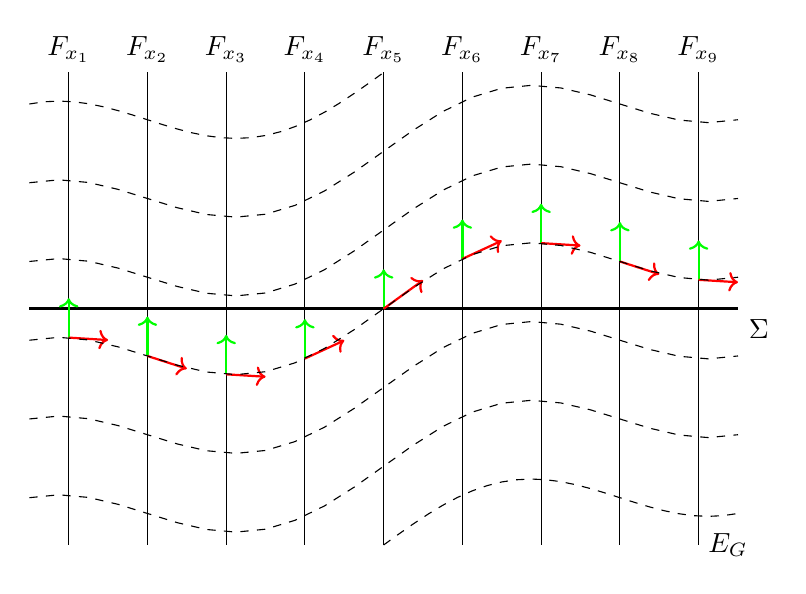
\begin{tikzpicture}[scale=0.5]
  \draw[very thick]
    (-9,0)
    --
    (9,0)
    node [below right] {$\Sigma$};
  \draw
    (-8,-6)
    --
    (-8,6)
    node [above] {$F_{x_{1}}$};
  \draw
    (-6,-6)
    --
    (-6,6)
    node [above] {$F_{x_{2}}$};
  \draw
    (-4,-6)
    --
    (-4,6)
    node [above] {$F_{x_{3}}$};
  \draw
    (-2,-6)
    --
    (-2,6)
    node [above] {$F_{x_{4}}$};
  \draw
    (0,-6)
    --
    (0,6)
    node [above] {$F_{x_{5}}$};
  \draw
    (2,-6)
    --
    (2,6)
    node [above] {$F_{x_{6}}$};
  \draw
    (4,-6)
    --
    (4,6)
    node [above] {$F_{x_{7}}$};
  \draw
    (6,-6)
    --
    (6,6)
    node [above] {$F_{x_{8}}$};
  \draw
    (8,-6)
    node [right] {$E_{G}$}
    --
    (8,6)
    node [above] {$F_{x_{9}}$};
  \draw[green,->,thick]
    (-8,{sin(-30*8)-8/5})
    --
    (-8,{sin(-30*8)-8/5+1});
  \draw[green,->,thick]
    (-6,{sin(-30*6)-6/5})
    --
    (-6,{sin(-30*6)-6/5+1});
  \draw[green,->,thick]
    (-4,{sin(-30*4)-4/5})
    --
    (-4,{sin(-30*4)-4/5+1});
  \draw[green,->,thick]
    (-2,{sin(-30*2)-2/5})
    --
    (-2,{sin(-30*2)-2/5+1});
  \draw[green,->,thick]
    (0,0)
    --
    (0,{sin(0)+1});
  \draw[green,->,thick]
    (2,{sin(30*2)+2/5})
    --
    (2,{sin(30*2)+2/5+1});
  \draw[green,->,thick]
    (4,{sin(30*4)+4/5})
    --
    (4,{sin(30*4)+4/5+1});
  \draw[green,->,thick]
    (6,{sin(30*6)+6/5})
    --
    (6,{sin(30*6)+6/5+1});
  \draw[green,->,thick]
    (8,{sin(30*8)+8/5})
    --
    (8,{sin(30*8)+8/5+1});
  \draw[red,->,thick]
    (-8,{sin(-30*8)-8/5})
    --
    ({-8+1},{30*pi*cos(-30*8)/180+1/5+sin(-30*8)-8/5});
  \draw[red,->,thick]
    (-6,{sin(-30*6)-6/5})
    --
    ({-6+1},{30*pi*cos(-30*6)/180+1/5+sin(-30*6)-6/5});
  \draw[red,->,thick]
    (-4,{sin(-30*4)-4/5})
    --
    ({-4+1},{30*pi*cos(-30*4)/180+1/5+sin(-30*4)-4/5});
  \draw[red,->,thick]
    (-2,{sin(-30*2)-2/5})
    --
    ({-2+1},{30*pi*cos(-30*2)/180+1/5+sin(-30*2)-2/5});
  \draw[red,->,thick]
    (0,0)
    --
    (1,{30*pi*cos(0)/180+1/5});
  \draw[red,->,thick]
    (2,{sin(30*2)+2/5})
    --
    ({2+1},{30*pi*cos(30*2)/180+1/5+sin(30*2)+2/5});
  \draw[red,->,thick]
    (4,{sin(30*4)+4/5})
    --
    ({4+1},{30*pi*cos(30*4)/180+1/5+sin(30*4)+4/5});
  \draw[red,->,thick]
    (6,{sin(30*6)+6/5})
    --
    ({6+1},{30*pi*cos(30*6)/180+1/5+sin(30*6)+6/5});
  \draw[red,->,thick]
    (8,{sin(30*8)+8/5})
    --
    ({8+1},{30*pi*cos(30*8)/180+1/5+sin(30*8)+8/5});
  \draw[dashed,domain=0:9]
    plot
    ({\x},{sin(30*\x)+\x/5-6});
  \draw[dashed,domain=-9:9]
    plot
    ({\x},{sin(30*\x)+\x/5-4});
  \draw[dashed,domain=-9:9]
    plot
    ({\x},{sin(30*\x)+\x/5-2});
  \draw[dashed,domain=-9:9]
    plot
    ({\x},{sin(30*\x)+\x/5});
  \draw[dashed,domain=-9:9]
    plot
    ({\x},{sin(30*\x)+\x/5+2});
  \draw[dashed,domain=-9:9]
    plot
    ({\x},{sin(30*\x)+\x/5+4});
  \draw[dashed,domain=-9:0]
    plot
    ({\x},{sin(30*\x)+\x/5+6});
\end{tikzpicture}
\]
The arrows in the picture hint at some equivalent characterizations of parallel transport. To understand this let us explain what the arrows mean. First of all, let us say that the green arrows parallel to the fibers should have been drawn at any crossing of fiber and dashed lines and not just for one of the dashed lines as well as the red arrows tangential to the dashed lines. For $e \in E_{G}$ let $T_{e}E_{G}$ denote the tangent space of $E_{G}$ at $e$.
\begin{enumerate}
\item[$\bullet$]
The green arrows should be understood symbolically as the subspace $V_{e}E_{G}$ of $T_{e}E_{G}$ which is tangential to the fiber, that is, the kernel of the tangent map $T_{e}\pi_{G} \colon T_{e}E_{G} \rightarrow T_{\pi_{G}(e)}\Sigma$ of $\pi_{G}$ (which is linear). $V_{e}E_{G}$ is referred to as vertical subspace and is independent of any parallel transport.
\item[$\bullet$]
The red arrows shall stand for the vector field on $E_{G}$ corresponding to the flow expressed by the dashed lines. So the red arrows are as good as the dashed lines here. Moreover we get dashed lines for any path in $\Sigma$ from a parallel transport and thus red arrows. All these red arrows at some $e \in E_{G}$ together span a subspace $H_{e}E_{G}$ of $T_{e}E_{G}$. $H_{e}E_{G}$ is referred to as horizontal subspace for the chosen parallel transport and hence depends on the chosen parallel transport. Moreover note that $H_{e}E_{G}$ gets along with the action on the fiber in the sense that the tangent map of the action maps horizontal spaces to horizontal spaces.
\end{enumerate}
What the picture now suggests is that given a parallel transport we have a direct sum decomposition
\begin{align*}
  T_{e}E_{G}
  &=
  V_{e}E_{G}
  \oplus
  H_{e}E_{G}
\end{align*}
such that the action on the fibers is respected. What we want to say is that instead of giving a parallel transport it suffices to (smoothly) specify $H_{e}E_{G}$ at each point of $E_{G}$ in a way that respects the action on the fiber.
\begin{enumerate}
\item[$\pmb{\hookrightarrow}$]
Mathematically, this smooth choice of horizontal space distribution is usually referred to as Ehresmann connection on $\pi_{G}$.
\end{enumerate}
This picture hopefully makes the terminology {\glqq}connection{\grqq} clear since it shall indicate how the fibers are {\glqq}connected{\grqq}. There is a convenient way to specify an Ehresmann connection. To this end consider the tangent bundles $\pi_{TE_{G}} \colon TE_{G} \rightarrow E_{G}$ and $\pi_{T\Sigma} \colon T\Sigma \rightarrow \Sigma$ on $E_{G}$ and $\Sigma$, respectively. We then have the vector bundle homomorphism
\begin{align*}
  T\pi_{G}
  :=
  (T_{e}\pi_{G})
  \colon
  TE_{G}
  &\rightarrow
  T\Sigma
\end{align*}
from $\pi_{G} \circ \pi_{TE_{G}}$ to $\pi_{T\Sigma}$ induced by the tangent maps $T_{e}\pi_{G}$. Now note that under factoring out the fiberwise action by $G$ from $E_{G}$ we get a unique vector bundle $\pi_{TE_{G}}^{!} \colon TE_{G} \slash G \rightarrow \Sigma$ with total space the quotient. Moreover the vector bundle homomorphism $T\pi_{G}$ induces a unique vector bundle homomorphism
\begin{align*}
  T\pi_{G}^{!}
  \colon
  TE_{G}
  \slash
  G
  &\rightarrow
  T\Sigma
\end{align*}
from $\pi_{TE_{G}}^{!}$ to $\pi_{T\Sigma}$. Now a smooth section $\sigma$ of $T_{e}\pi_{G}$ which is linear, that is, a linear map
\begin{align*}
  \sigma
  \colon
  T_{\pi_{G}(e)}\Sigma
  &\rightarrow
  T_{e}E_{G}
\end{align*}
such that $T_{e}\pi_{G} \circ \sigma$ is the identity, can be shown to already determine a horizontal subspace using the fact that $\sigma$ as linear section maps only the $0$ to the vertical subspace. Moreover, because it essentially suffices to determine one horizontal subspace in each fiber due to the compatibility with the action, an Ehresmann connection on $\pi_{G}$ can be seen to correspond precisely to a smooth section of $T\pi_{G}^{!}$, considered as homomorphism of vector bundles. So to define an Ehresmann connection on $\pi_{G}$ we can provide a certain family of linear maps
\begin{align*}
  \sigma_{x}
  \colon
  T_{x}\Sigma
  &\rightarrow
  \left(
    \pi_{TE_{G}}^{!}
  \right)^{-1}
  (x)
\end{align*}
smoothly depending on $x$. In other words: an Ehresmann connection is nothing but a smooth section of the \textit{homomorphism bundle for $\pi_{G}$} which is just the tensor bundle
\begin{align*}
  \pi_{T\Sigma}^{\prime}
  \otimes
  \pi_{TE_{G}}^{!}
  \colon
  E_{\pi_{G}}
  &\rightarrow
  \Sigma
\end{align*}
where $\pi_{T\Sigma}^{\prime}$ is the fiberwise vector space dual to $\pi_{T\Sigma}$ and $\sigma_{x}$ is then an element (up to isomorphism from tensoring) of a fiber of this bundle. So a connection can be regarded as a section of a fiber bundle. Namely one with fiber the vector space of some vector space homomorphisms. But there is still another convenient characterization of the idea described so far. This arises from the Ehresmann connection in the following way. Because $V_{e}E_{G}$ is regarded as being tangential to the fiber and the fiber is isomorphic to the Lie group $G$ the vertical subspace $V_{e}E_{G}$ should be isomorphic to the Lie algebra $\mathrm{Lie}_{G}$ of $G$ which is by definition just the tangent space at the identity element of the Lie group. Given an Ehresmann connection we can now map any vector in $T_{e}E_{G}$ to its $V_{e}E_{G}$ component such that this function gets along with the action in some sense. What we then get in the end is essentially a Lie algebra-valued $1$-form subjected to some properties.
\begin{enumerate}
\item[$\pmb{\hookrightarrow}$]
Mathematically, this Lie algebra-valued $1$-form with its properties is usually referred to as principal connection on $\pi_{G}$.
\end{enumerate}
For the record:
\begin{enumerate}
\item[$\pmb{\hookrightarrow}$]
Mathematically, we have an equivalence of
\begin{enumerate}
\item[$\bullet$]
Parallel Transport for $\pi_{G}$
\item[$\bullet$]
Ehresmann Connection on $\pi_{G}$
\item[$\bullet$]
Principal Connection on $\pi_{G}$
\end{enumerate}
This equivalence can be found to some extent in \cite{797789bc}. More on this (including sources) can also be found in \cite{wiki-nlab0000}: connection on a bundle.
\end{enumerate}
Note that whenever we are given an action $\mathrm{a}_{F}$ of $G$ on a smooth manifold $F$ then we can loosely speaking replace each fiber $F_{x}$ of $\pi_{G}$ by $F$ to get a fiber bundle $\pi_{\mathrm{a}_{F}}$ over $\Sigma$. And then each parallel transport induces such a notion in $\pi_{\mathrm{a}_{F}}$. If further $F$ is a vector space this parallel transport allows to define a differential quotient.
\begin{enumerate}
\item[$\pmb{\hookrightarrow}$]
Mathematically, we are talking about the bundle associated with $\pi_{G}$ via an action of $G$ on $F$ and in case of $F$ a vector space the covariant derivative for the parallel transport. The covariant derivative in an associated vector bundle is a coordinate free way of measuring change of sections in this bundle along vector fields. Details can be found in \cite{797789bc}.
\end{enumerate}
So whenever we have sections of a vector bundle associated with a principal bundle governing a local symmetry we should use the covariant derivative w.r.t. this symmetry when we have to determine the change of such a section in spacetime to get along with the symmetry. Now as it is instructive to understand a manifold in local coordinates we expect this to be interesting in the case of a bundle, too. So let $s \colon U \rightarrow E_{G}$ be a smooth local section of the $G$-principal bundle $\pi_{G}$ on which we have a principal connection $\omega$. We can use the tangent map of $s$ to map a tangent vector of $U$ to one of $E_{G}$ to which we can then apply $\omega$ to get a vector in the Lie algebra. So, locally, we expect to get a Lie algebra-valued $1$-form $s^{\ast}(\omega)$ on $U$ from $\omega$ depending on the chosen section $s$. And choosing coordinates $q_{\varphi}^{i}$ for $U$ we can write
\begin{align*}
  s^{\ast}(\omega)(x)
  &=
  \sum_{i=0}^{n}
  A_{q_{\varphi}^{i}}^{s}(x)
  \mathrm{d}q_{\varphi}^{i}(x)
\end{align*}
here with functions $A_{q_{\varphi}^{i}}^{s} \colon U \rightarrow \mathrm{Lie}_{G}$ (depending on the choice of $s$).
\begin{enumerate}
\item[$\pmb{\hookrightarrow}$]
Mathematically, $s^{\ast}(\omega)$ is the pullback of $\omega$ along $s$ and this can be regarded as a smooth local section of the cotangent bundle tensored with the Lie algebra of $G$ which then i.p. results in a vector bundle.
\end{enumerate}
This is a neat simplification of the connection (locally) and it is an interesting question if we can reconstruct $\omega$ from such local data on $\Sigma$. So assuming a set $K$ and smooth local sections $s_{k} \colon U_{k} \rightarrow E_{G}$ of $\pi_{G}$ for all $k \in K$ trivializing all of $\pi_{G}$ this is to say: can we reconstruct $\omega$ from all the local Lie algebra-valued one forms $s_{k}^{\ast}(\omega)$ on $U_{k}$? To answer this question it seems that one should understand what happens on $U_{k_{1}} \cap U_{k_{2}}$ for $(k_{1},k_{2}) \in K \times K$. So we should stick with the coordinate approach and see what a change of local coordinates does. First note that for smooth local sections $s_{1} \colon U_{1} \rightarrow E_{G}$ and $s_{2} \colon U_{2} \rightarrow E_{G}$ of $\pi_{G}$ we have for each $x \in U_{k_{1}} \cap U_{k_{2}}$ a unique $g_{x} \in G$ such that
\begin{align*}
  s_{2}(x)
  &=
  \mathrm{a}_{x}
  \left(
    g_{x},
    s_{1}(x)
  \right)
\end{align*}
due to the free transitivity of the action $\mathrm{a}_{x}$ on the fiber $F_{x}$ of $\pi_{G}$. Then the change of coordinates from $s_{1}$ to $s_{2}$ corresponds precisely to the smooth function
\begin{align*}
  \tau_{s_{1},s_{2}}
  \colon
  U_{k_{1}}
  \cap
  U_{k_{2}}
  &\rightarrow
  G
  \\
  x
  &\mapsto
  g_{x}
\end{align*}
called transition function. Moreover note that there is an explicit formula - let us label this $\mathfrak{F}_{q_{\varphi}^{i}}^{s_{1},s_{2}}(\omega)$ for the sake of easy reference here - relating $A_{q_{\varphi}^{i}}^{s_{1}}(x)$ and $A_{q_{\varphi}^{i}}^{s_{2}}(x)$ for all $x \in U_{1} \cap U_{2}$ using the transition function $\tau_{s_{1},s_{2}}$. For details see \cite{797789bc}. However, we will later write this formula down in the case of matrix groups. Now back to the trivializing sections $s_{k}$. Then for all pairs $(k_{1},k_{2}) \in K \times K$ we have transition functions $\tau_{s_{k_{1}},s_{k_{2}}}$ and these satisfy the cocycle condition\footnote{yes this has to do with cohomology as we will see more explicitly later in chapter \ref{chap:cattg}}
\begin{align*}
  \tau_{s_{k_{1}},s_{k_{2}}}(x)
  \cdot
  \tau_{s_{k_{2}},s_{k_{3}}}(x)
  &=
  \tau_{s_{k_{1}},s_{k_{3}}}(x)
\end{align*}
for all suited $x$ and all possible combinations of $k_{1},k_{2},k_{3} \in K$. This in particular implies
\begin{align*}
  \tau_{s_{k},s_{k}}(x)
  &=
  e_{G}
  \\
  \tau_{s_{k_{1}},s_{k_{2}}}(x) 
  &=
  \tau_{s_{k_{2}},s_{k_{1}}}(x)^{-1}
\end{align*}
where $e_{G}$ denotes the identity element of $G$. One can show that from this data - the transition functions satisfying the cocycle condition - $\pi_{G}$ is reconstructable up to isomorphism. One can even show that functions $A_{q_{\varphi}^{i}}^{s_{k}} \colon U_{k} \rightarrow \mathrm{Lie}_{G}$ pairwise related by $\mathfrak{F}_{q_{\varphi}^{i}}^{s_{k_{1}},s_{k_{2}}}(\omega)$ on overlaps patch together to a unique connection on $\pi_{G}$. So the $s_{k}^{\ast}(\omega)$ already determine the connection. Now assume further smooth local sections $s_{k}^{\backprime} \colon U_{k} \rightarrow E_{G}$ of $\pi_{G}$ for all $k \in K$ trivializing all of $\pi_{G}$. Then there are unique smooth functions
\begin{align*}
  f_{s_{k},s_{k}^{\backprime}}
  \colon
  U_{k}
  &\rightarrow
  G
\end{align*}
satisfying the coboundary condition
\begin{align*}
  f_{s_{k_{1}},s_{k_{1}}^{\backprime}}(x)
  \cdot
  \tau_{s_{k_{1}}^{\backprime},s_{k_{2}}^{\backprime}}(x)
  &=
  \tau_{s_{k_{1}},s_{k_{2}}}(x)
  \cdot
  f_{s_{k_{2}},s_{k_{2}}^{\backprime}}(x)
\end{align*}
for all suited $x$. One can then show that the bundle reconstructed from the $s_{k}$ is isomorphic to the bundle reconstructed from the $s_{k}^{\backprime}$ using the $f_{k}$ satisfying the coboundary condition. This in particular shows that a change of coordinates from $s_{k}$ to $s_{k}^{\prime}$ originates from a $G$-principle bundle isomorphism $\Phi$ from $\pi_{G}$ to $\pi_{G}$. Note that the pullback $\Phi^{\ast}(\omega)$ of a principal connection $\omega$ is also a principal connection. And the connection $\Phi^{\ast}(\omega)$ in the coordinates $s_{k}$ is the same as $\omega$ in coordinates $\Phi \circ s_{k}$.\footnote{this is since pulling back essentially respects composition contravariantly as you will know after chapter \ref{chap:cattg}} On the other hand, $f_{s_{k},s_{k}^{\backprime}}$ is what we actually wanted as change of perspective respecting the principle of locality. So in the end, if we change local coordinates of the physical situation we are looking at we must change local coordinates of the connection at the same time. The common ground of these changes is the isomorphism $\Phi$. Thus it seems better to regard the isomorphisms of the bundle as actual changes of perspective. Let us run through an easy class of examples which cover most physically relevant cases. Namely $G$ as a sub Lie group of the $n$-dimensional general linear group $GL(n,\mathbb{K})$ with coefficients in $\mathbb{K} = \mathbb{R},\mathbb{C}$. The Lie algebra $\mathrm{Lie}_{G}$ is then also a matrix group and for an isomorphism $\Phi$ and local coordinates $s$ we have
\begin{align*}
  (\Phi \circ s)(x)
  &=
  \tau_{s,\Phi \circ s}(x)
  \cdot
  s(x)
  \\
  A_{q_{\varphi}^{i}}^{\Phi \circ s}(x)
  &=
  \tau_{s,\Phi \circ s}(x)
  \cdot
  A_{q_{\varphi}^{i}}^{s}(x)
  \cdot
  \tau_{s,\Phi \circ s}(x)^{-1}
  +
  \tau_{s,\Phi \circ s}(x)
  \cdot
  \partial_{q_{\varphi}^{i}(x)}
  \tau_{s,\Phi \circ s}(x)^{-1}
\end{align*}
according to \cite{797789bc}. In particular, for $G = U(1)$ the $1$-dimensional unitary group, which geometrically as a manifold is nothing but a circle, the Lie algebra $\mathrm{Lie}_{U(1)}$ is isomorphic to $\mathbb{R}$ as vector space and we have
\begin{align*}
  (\Phi \circ s)(x)
  &=
  \mathrm{exp}(\mathrm{i}\theta_{\Phi}(x))
  \cdot
  s(x)
  \\
  A_{q_{\varphi}^{i}}^{\Phi \circ s}(x)
  &=
  A_{q_{\varphi}^{i}}^{s}(x)
  +
  \partial_{q_{\varphi}^{i}(x)}
  \theta_{\Phi}(x)^{-1}
\end{align*}
Moreover for the action
\begin{align*}
  \mathrm{a}_{\mathbb{C}^{n}}
  \colon
  U(1)
  \times
  \mathbb{C}^{n}
  &\rightarrow
  \mathbb{C}^{n}
  \\
  (\mathrm{exp}(\mathrm{i}\theta),z)
  &\mapsto
  \mathrm{exp}(\mathrm{i}\theta)
  \cdot
  z
\end{align*}
where $\cdot$ means scalar multiplication and a smooth section $\phi$ of the vector bundle $\pi_{\mathbb{C}^{n}}$ associated with $\pi_{U(1)}$ via $\mathrm{a}_{\mathbb{C}^{n}}$ the covariant derivative $D_{q_{\varphi}^{i}(x)}^{s}$ of $\phi$ in the chosen coordinates is given by
\begin{align*}
  \left(
    D_{q_{\varphi}^{i}(x)}^{s}
    \phi
  \right)
  (x)
  &=
  \left(
    \partial_{q_{\varphi}^{i}(z)}
    \phi
  \right)
  (x)
  +
  A_{q_{\varphi}^{i}}^{s}(x)
  \cdot
  \phi(x)
\end{align*}
Let us summerize what we have done here. We proposed a mathemtical description of a physical situation which is the same under different viewpoints and respects the principle of locality. Then from the desire to compare for changes at near points in spacetime we predicted the need of a section of some fiber bundle (namely the connection $\omega$) from purely geometrical considerations. And the view on this section depends on the view on the physical situation. So one might conjecture that this section is somehow influenced (at least) by the sole presence of the physical situation.
\item[(4)]
Physical quantities are often described as things on spacetime. Just think of
\begin{enumerate}
\item[$\bullet$]
semi-Riemannian metrics in GR
\item[$\bullet$]
potentials in electrodynamics\footnote{usually only for $\Sigma = \mathbb{R}^{4}$ as Minkowski spacetime but possibly also on arbitrary spacetimes}
\item[$\bullet$]
wave functions in relativistic quantum mechanics\footnote{usually only for $\Sigma = \mathbb{R}^{4}$ Minkowski spacetime} (Klein-Gordon and Dirac equation)
\end{enumerate}
which already covers a significant part of traditional\footnote{from the first half of the 20th century} physics. We go into more detail in a moment. But first some terminological settlements. The physical quantities we are talking about are usually called fields or field configurations and one can take the stance that (theoretical) physics is all about the description of fields from a nowadays perspective.
\begin{enumerate}
\item[$\pmb{\hookrightarrow}$]
Mathematically, a field should be smooth section of a smooth fiber bundle\footnote{we assume those locally trivial by definition} over spacetime $\Sigma$.
\end{enumerate}
In physics, one calls a fiber bundle over spacetime
\begin{align*}
  \pi
  \colon
  E_{\pi}
  &\rightarrow
  \Sigma
\end{align*}
with fiber $F_{\pi}$ field bundle while the fiber of this bundle is called field fiber and is often denoted $\mathrm{Conf}_{\pi} := F_{\pi}$. The space of smooth sections of the bundle $\pi$ is denoted
\begin{align*}
  \Gamma_{\pi}^{\mathrm{glob}}
\end{align*}
and called field configuration space. A point of this space is consequently called a field configuration. If $U$ is a subspace of $\Sigma$ then we have a smooth fiber bundle
\begin{align*}
  \pi
  \vert
  U
  \colon
  \pi^{-1}(U)
  &\rightarrow
  U
  \\
  e
  &\mapsto
  \pi(e)
\end{align*}
and hence we can define
\begin{align*}
  \Gamma_{\pi}(U)
  &:=
  \Gamma_{\pi \vert U}^{\mathrm{glob}}
\end{align*}
which are the local sections of $\pi$ over $U$ and are called local field configurations. The principle of locality suggets that for any cover of $\Sigma$ by subspaces we should be able to uniquely construct a field configuartion from local ones which match on overlaps.
\begin{enumerate}
\item[$\pmb{\hookrightarrow}$]
Mathematically, this means that $\Gamma_{\pi}$ should be something like a sheaf\footnote{a not so small part of chapter \ref{chap:cattg} is ultimately about sheaves (including motivation and a formal definition)}.
\end{enumerate}
So what actually matters when we demand the principal of locality is $\Gamma_{\pi}$ and not so much the field bundle. Note that if moreover $U$ is such that $\pi$ is trivial over it then restricting a field configuration from $\Gamma_{\pi}^{\mathrm{glob}}$ to $U$ can be considered a function from $U$ to $\mathrm{Conf}_{\pi}$ since
\begin{align*}
  (\pi \vert U)^{-1}(U)
  &\cong
  U
  \times
  \mathrm{Conf}_{\pi}
\end{align*}
And if we even have charts with domain $U$ then, locally, a field configuration can be considered a function from $\mathbb{R}^{n+1}$ to $\mathrm{Conf}_{\pi}$. Note that fields are often defined as such functions or perhaps more generally as functions from $\Sigma$ to $\mathrm{Conf}_{\pi}$. In our language this is to say that fields are defined to be trivial bundles. While this is appropriate for electrodynamics and relativistic quantum mechanics to some extent it does not make sense for GR whose metric is a tensorfield over spacetime which is a section of a certain fiber bundle in general. Anyways, the interpretation of fields as sections through bundles implies that connections on principal bundles are fields since they can be regarded as sections through the homomorphism bundle
\begin{align*}
  \pi_{T\Sigma}^{\prime}
  \otimes
  \pi_{TE_{G}}^{!}
  \colon
  E_{\pi_{G}}
  &\rightarrow
  \Sigma
\end{align*}
from above. This qualifies the connections to have a physical meaning which even seems natural since we predicted them from a physical desire. And not only this, we can patch the connection $\omega$ together from local fields $s_{k}^{\ast}(\omega)$ when we track the symmetry transformations. However, we lack an interpretation so far. So let us look at our initial examples of point (3). Both of these are a bit unrealistic in the light of GR and relativistic quantum mechanics. So let us take a closer look.
\begin{enumerate}
\item[$\bullet$]
In GR we do not only assume spacetime to be a smooth manifold but we also assume a semi-Riemannian metric on it among other things. And this demand has to be compatible with general covariance. In the end one is more or less forced to take the Levi-Civita connection on the frame bundle $\pi_{GL(n+1)}$ over spacetime $\Sigma$ for the purpose of GR. This connection is uniquely determined by the semi-Riemannian metric. So the covariant derivative of GR in any associated bundle (i.p. tensor bundles) is the one obtained from the Levi-Civita connection. In GR all relevant fields are sections of such associated bundles. The $A_{q_{\varphi}^{i}}^{s}(x)$ are known as Christoffel symbols. Note that if we take $\Sigma = \mathbb{R}^{4}$ as Minkowski spacetime we get the ordinary derivative from the Levi-Civita connection since we have global sections of the principal bundle in this case.
\item[$\bullet$]
If anything is a field on spacetime then also a massive particle with internal symmetry ought to be so. So take a relativistic electron with spin $\psi \colon \mathbb{R}^{4} \rightarrow \mathbb{C}^{4}$ as solution of the Dirac equation, for example. This can be regarded as a section of the bundle associated to the trivial $U(1)$-bundle via $\mathrm{a}_{\mathbb{C}^{4}}$ from point (3). Now the electron must influence the connection and the obvious thing an electron influences is the electromagnetic field. But the electromagnetic field is a $2$-form while the connection is a Lie alegebra-valued $1$-form here. However, the potential of the electromagnetic field can be considered as such. So one might conjecture that the predicted section (the connection) is the potential generated by the electron. This is further underpinned by the behaviour of $A_{q_{\varphi}^{i}}^{s}$ under symmetry transformations. But note that the Maxwell equations for the potential have vacuum solutions and one has to take these into account for the connection, too, then. This is the idea of quantum electrodynamics (abbr. QED). More generally, this suggests that a massive particle with internal symmetry a Lie group $G$ is a section of a bundle associated with a $G$-principal bundle over Minkowski spacetime governing the symmetry while the connections on this bundle are the fields of the potential of the predicted fundamental force which also has vacuum solutions. This idea was very successful in that three of the four known fundamental forces (all but the gravitational force) were combined into the SMP with a single Lie group $G_{\textrm{SMP}}$. So to understand the SMP locally we have to look at $G_{\textrm{SMP}}$-principal bundles over Minkowski spacetime and connections on it. But we want to understand it globally so we should look at principal bundles over any spacetime $\Sigma$ and connections on it, as well as sections through associated bundles and their covariant derivatives in case of vector bundles.
\end{enumerate}
Physically, a major reason of why to take arbitrary principle bundles into account (and hence a further reason for arbitrary field bundles) is that the principal bundle twists encode the theoretically important \textit{instantons} which are for instance relevant to understand the vacuum state of the SMP. The bundle twists depend only on the isomorphism class of the principal bundle and people are tempted to factor isomorphism out. This thinking arises from an often unrecognized misconception regarding symmetry and redundancy. On the philosophical level: symmetry is not the same as redundancy. Symmetry means that we can look at a situation from different perspectives without observing a difference in the situation but this does not imply that we can identify these perspectives with each other to one single perspective. This would collapse the symmetry information and we would hence lose information which we would not if we had redundancy. The physical argument against this is that if we collapse the symmetry information then we can only regain $\omega$ from the local data $s_{k}^{\ast}(\omega)$ if $\pi_{G}$ is trivial and hence allows for a (global) smooth section. So we would have to give up the principle of locality or instantons. Or we just allow to track the symmetry in the definition of field. This is to say that we map any patch $U$ of spacetime to the collection of $G$-principle bundles over $U$ with connection structured by bundle isomorphisms preserving the connection. Additionally, we require that we can uniquely glue things together on overlaps.
\begin{enumerate}
\item[$\pmb{\hookrightarrow}$]
Mathematically, the structured collection is a groupoid - which is actually a homotopy $1$-type - while mapping the patches to these groupoids under such a condition is a stack (kind of a weakened sheaf in some sense usually expressed as groupoid-valued functor). If one develops this idea further with symmetry of symmetry\footnote{this can be important in string theory} and so on then one ends up with $\infty$-groupoids - which capture the full homotopy of topological spaces (Grothendieck hypothesis) - and $\infty$-stacks (kind of sheaf up to homotopy in some sense usually expressed as $\infty$-groupoid-valued functor). So it seems reasonable to model physical fields obeying the principle of locality as $\infty$-stacks.
\end{enumerate}
For more on this see \cite{d1ad46b9} and \cite{wiki-nlab0000}: field (physics). After all we see that homotopy theory and category theory\footnote{e.g. the functors here} are important in physics. But stacks are not the only point where homotopical properties matter in physics. For instance, the parallel transport depends on the homotopy class of the path. And the Berry phase of an electron we mentioned earlier has its origin in an electron moving around a homotopically non-trivial path. But homotopy theory has much to do with category theory as we hinted earlier and so we have another way how category theory becomes important to physics. And this is still not all: Let $X$ be a CW complex then - when we require only continuous instead of smooth - an isomorphism class of $G$-principal bundles over $X$ corresponds precisely to a homotopy class of maps from $X$ to a CW complex $\mathrm{B}G$ obtained from $G$ which in turn corresponds to a cohomology class in the first cohomology\footnote{singular if $G$ is abelian} group with coefficients in $G$.\footnote{for the latter we should take basepoints into account} We write this boldly as
\begin{align*}
  \mathcal{P}_{G}(X)
  &\cong
  \mathrm{hom}_{\mathrm{Ho}(\mathbf{Top}_{\ast}^{\textrm{CW}})}
  \left(
    X,
    \mathrm{B}G
  \right)
  \cong
  h_{G}^{1}(X)
\end{align*}
It needs much of chapter \ref{chap:cattg} to understand this categorically even though we do not really prove it in full generality. Unfortunately, this classification does not work for isomorphism classes of principle bundles over a manifold with connection. But there is a way around this by replacing smooth manifolds with a more general kind of space. These generalized spaces will be a recurring example in chapter \ref{chap:cattg}. The only problem left are then the isomorphism classes where we actually should use higher groupoids.
\item[(5)]
The physical laws which govern the field configuration can often be obtained from a Lagrangian density for the field configuration by Hamilton's principle. Examples include:
\begin{enumerate}
\item[$\bullet$]
Einstein's field equations for semi-Riemannian metrics in GR
\item[$\bullet$]
Maxwell's equations for potentials in electrodynamics\footnote{usually only on Minkowski spacetime}
\item[$\bullet$]
Klein-Gordon and Dirac equation for wave functions in relativistic quantum mechanics\footnote{usually only on Minkowski spacetime}
\end{enumerate}
So the Lagrangian density for the field is assumed to contain much (if not all) information about the considered physical system. But one has to take care to take the right covariant derivative if necessary to incorporate the right local symmetry into the Lagrangian. For example, the QED Lagrangian on Minkowski spacetime is the sum of the vacuum electrodynamics Lagrangian and the Dirac Lagrangian where the latter uses the covariant derivative w.r.t. the symmetry of the electron which then results in an interaction of electron and electromagnetic field. Moreover note that if one further wants to incorporate the principal of locality here then the Lagrangian density for the field on a local patch of spacetime should in some way be independent of that on some disjoint patch. So one should actually take the local Lagrangian density.
\begin{enumerate}
\item[$\pmb{\hookrightarrow}$]
Mathematically, this is modelled as a horizontal differential form of degree the dimension of spacetime on the jet-bundle for the field bundle.
\end{enumerate}
We do not explain here what this is. Let us just say that, locally, on $U$ one gets what one would usually understand as Lagrangian density.
\end{enumerate}
So far we have actually only taken GR into acount but not quantum theory which is also a pillar of physics. To incorporate quantum theory one has to quantize the classical fields we described so far. This is one of the main problems of physics at the moment. One wants to find a process of getting a formal quantum field theory (abbr. QFT) from the classical field theory (fields and local Lagrangian densities) such as Feynman's path intgrals which are quite succesful but not mathematically rigorous. The processes of quantization are more thoroughly discussed in \cite{00000011}. There are essentially two mathematical approaches for formal QFTs: algebraic quantum field theory (abbr. AQFT) and functorial quantum field theory (abbr. FQFT).
\begin{enumerate}
\item[$\bullet$]
AQFT is the approach preferred by most mathematical physicists. The idea is to cover spacetime by subspaces each coming with an operator algebra made up by the observable physical quantities on this subspace. On overlaps the observables are expected to get along with each other in some sense. There are two well-known proposals for axiomatizations.\footnote{we want to emphasize the word {\glqq}proposal{\grqq} here} The Wightman axioms and the Haag-Kastler axioms, respectively. We do not want to go into detail here. We do not further discuss AQFTs here at all. We only want to say that the connection to category theory does not look so deep here. At least at first glance at which it seems as category theory would only provide a convenient language in some places in the guise of presheaves. Presheaves will play a major role in chapter \ref{chap:cattg} as you will see.
\item[$\bullet$]
FQFT is the approach which is obviously pure category theory. An FQFT is a (higher) {\glqq}functor{\grqq} from a certain geometric (higher) category to a certain algebraic (higher) category. A (higher) functor can be understood as higher-dimensional function if higher categories are considered higher dimensional sets. This is to say if a higher category is made up by countably many levels then a higher functor maps levels of some rank to levels of the same rank. If you do not understand this yet we guarantee you will after reading chapter \ref{chap:cattg}. Unfortunately, it is not yet known what the correct categories are. While the geometric domain category has to do with cobordisms as is more or less clear the algebraic one makes more problems. But there is a special case which is better understood: topological quantum field theory (abbr. TQFT). These are quantum field theories not depending on the metric of spacetime but rather on the geometry of it. TQFTs are a sort of reasonably formalized FQFTs. We will roughly sketch what a TQFT categorically is in chapter \ref{chap:cattg} but then refer to \cite{00000011} which precisely defines them together with a motivation from Feynman's path integrals.
\end{enumerate}
AQFT and FQFT can be understood as dual\footnote{roughly: the same from different perspectives} to each other in the sense that algebra and geometry can be understood as dual to each other.\footnote{This is captured by so-called Isbell duality in category theory and can be traced back to Grothendiecks functorial geometry over Lawvere's idea of a duality of generalized space - a recurring example in chapter \ref{chap:cattg} and quantity. However, we will neither prove nor state Isbell duality in these notes.} In physics this manifests itself in the Heisenberg picture which is known as the algebraic point of view on quantum mechanics and the Schr\"odinger picture which is known as the geometric point of view on quantum mechanics.
\\\\
Finally note, that in \cite{wiki-nlab0000} they more or less say a gauge theory is a \textit{QFT} whose \textit{field configurations} are \textit{principal bundles with connection}. So this section was ultimately all about higher category in gauge theory which is a dominant field of research in modern physics.




\chapter{Category Theory Interpreted in TG}
\label{chap:cattg}
\stepcounter{prpcounter}
This is the main - and by far the longest - chapter of these notes. It is all about category theory (as mathematical theory) with little attention on physics. However we will develop it in a potential mathematical theory of everthing: Tarski-Grothendieck set theory. TG is (almost) ordinary mathematics as you might know it.\footnote{see appendix \ref{chap:tg} for this} Moreover we pay special attention to homotopy theory and higher category theory albeit on a way more informal level than we do for ordinary category theory. Homotopy theory and higher category theory will play a role in almost any section of this chapter. But let us emphasize that it should be possible to understand a good part of this chapter without any prior knowledge of these theories (i.p. homotopy theory). Actually, it should suffice to know some basic set theoretical constructions (unions, instersections, relations, functions, \ldots), ordered sets (pre, partially, totally, well) and a bit about equivalence relations.
\\\\
Let us now talk a bit about the sections of this chapter. Of course, we present the most basic ideas of category theory as you would find them in any text about general category theory but with certain emphases which are not so standard. Let us present this as a list:
\begin{enumerate}
\item[$\bullet$]
The trinity in section \ref{sec:trinity}: categories, functors, natural transformations. What is perhaps special in our notes is the early focus on higher categories which we already introduce in the trinity section \ref{sec:trinity}. We will then later see that this trinity is not so {\glqq}holy{\grqq} as one might guess from from a first glance at category theory but rather an expression of the fact that $0$ and $1$ and $2$ are three natural numbers. 
\item[$\bullet$]
Duality in section \ref{sec:duality}. This is actually addressed in any serious text about category theory since a lack of understanding this can make things a little bloated. Therefore we tried to emphasize this thorughout these notes as much as possible.
\item[$\bullet$]
Constructions on a category in section \ref{sec:constoncat}. We only discussed the ones important to us: product categories and comma categories. There are quite a few more interesting ones we do not discuss such as graphs. For this section there are certainly more complete sources.
\item[$\bullet$]
Universality in section \ref{sec:uni}. This is the most important thing about category theory which is why we extensively discuss it. We strived to be as intuitive as possible (what we actually try throughout the whole notes) with a special interest on parts which are particularly important to physicist (but for mathematicians as well). We start from what {\glqq}universality{\grqq} intuitively means followed by the far reaching Yoneda lemma waiting there for us. It is not exaggerated to say that the Yoneda lemma dominates category in some sense. You will hopefully comprehend what we mean after a perusal of section \ref{sec:uni}. With limits and adjoints we will get to know the arguably most common {\glqq}universal constructions{\grqq}. We will prove most of the standard theorems for those. Then a bit hidden in a subsubsection with Kan extension we get to know a further universal construction which is also of major importance. Especially in homotopy theory they play a role.\footnote{we will later see this more explicity when considering simplicial sets in section \ref{sec:sset}} So be warned and do not underrate the subsubsection \ref{sec:coyoneda2}.
\end{enumerate}
Well, this is what we consider the basics of category theory.
\\
After this basics it is time to look a bit at the big picture of category theory from a modern\footnote{the authors are not full-fledged researchers - so do not expect too much} perspective. This is done in one section with a somewhat obscure title:
\begin{enumerate}
\item[$\bullet$]
Meta-ideas in section \ref{sec:metaidea}. Category theory and especially higher category theory is surrounded by many more or less informal ideas (therefore meta-ideas). We try to present these in a more or less informal style depending on how sophisticated the idea is and how much effort is acceptable for our purposes. The section is full of examples some of which are very important to us while others might be only for illustrative purposes. But almost anything we discuss in this section has more or less direct applications in physics. In particular, we define principal bundles and discuss them the more general setting of (higher) topoi.
\end{enumerate}
This should complete an informal introduction to higher category theory with many references interesting in this direction.
\\
The last two sections are closely related to homotopy theory. And since homotopy theory is very important in our context we pay more attention to the subject than the ordinary introductory texts on category theory. Let us briefly discuss the topics we mean.
\begin{enumerate}
\item[$\bullet$]
Simplicial sets in section \ref{sec:sset}. In this section we discuss how simplicial sets play a major role in homotopy theory (even more than one would expect as from a better version of simplicial complexes). In particular, we discuss how to use them in the classification of principal bundles by homotopy classes and cohomology ({\glqq}calculated{\grqq} with \v{C}ech cohomology).
\item[$\bullet$]
Fibrations in section \ref{sec:fibration}. For an algebraic topologist or even classical homotopy theorist it is obvious that this has to do with homotopy theory. We discuss a very general idea of fibrations and their duals (cofibrations) encompassing the notions from classical homotopy theory. The highlight\footnote{not only of this section} is astonishingly a pretty formal definition of {\glqq}stack{\grqq}. These homotopy-theortic versions of sheaves\footnote{defined somewhere in section \ref{sec:uni}} seem to be the proposed mathmatical objects containing the information of physical fields in quantum field theory obeying the principle of locality.
\end{enumerate}
We hope we made it to give a reasonable overview of this chapter to save you from missing the forest for the trees.



\section{The Trinity}
\label{sec:trinity}
Historically, Eilenberg and Mac Lane observed that some functions in algebraic topology were more than mere functions. These functions commuted with a certain kind of transformation - namely the natural transformations which we introduce in subsection \ref{sec:nt}. This naturality property is often necessary in algebraic topology to make things work. Anyways, to precisely formulate what they meant they needed the notion of categories as auxiliary concept. But actually they gave birth to a new theory. Category Theory. While introducing categories from this perspective seems intuitive for algebraic topologists and is, in fact, often introduced in this way there, it is not really helpful for anyone else. Even an algebraic topologist will eventually gain from the more modern approach we present. At some point in history people observed that a category defined as a certain set\footnote{as usual in mathematics} is an interpretation of some first order-theory - called category theory - in set theory. Hence categories make sense without any surrounding set theory. This is the addressed more modern approach and we will see that it is way more fundamental as the fact that it is a deductive system already suggests.
\\
Remember that in a set theory such as Zermelo-Fraenkel set theory with choice (abbr. ZFC) or Tarski-Grothendieck set theory (abbr. TG) the idea is that the only mathematical objects inhabiting the mathematical universe are sets. Preformally, a set is seen as a collection of things. Set theories like ZFC or TG do not directly say what a set is but they rather characterize them by their properties.\footnote{but rememeber G\"odel's incompleteness theorems} ZFC and TG for example say that given two sets we can test if one set is in the collection made up by the other set. This testing is the (by mathematicians) well-known binary relation {\glqq}is element of{\grqq} $\in$ and ZFC and TG, respectively, is a list of intuitively (more or less) sensible assumptions which govern the relation $\in$ and the mathematical universe.
\\
Directed paths - that is, paths which can be gone only in one direction - are for category theory what sets are for ZFC and TG. So, in category theory, we consider directed paths as the only mathematical objects inhabiting the mathematical universe. Now what is special about the directed path we have in mind. How can we characterize directed paths? First of all, we symbolize a directed path by an arrow\footnote{indeed, some use the notion of arrows here rather than this of directed paths as we do}
\begin{align*}
  \longrightarrow
\end{align*}
Certainly a directed path has two different ends. Namely
\begin{enumerate}
\item[(1)]
a starting point - a source from which the arrow points away
\item[(2)]
a terminus (an ending point) - a target to which the arrow points.
\end{enumerate}
If a directed path starts where another one ends we consider it sensible to be able to patch these directed paths together to a single directed path. That is, we want to be able to compose directed paths. In an arrow picture:
\[
\begin{tikzcd}[sep=large]
  \phantom{1}
  \arrow[shift left=1ex]{r}{}
  \arrow[shift right=1ex]{rr}{}
  &
  \phantom{1}
  \arrow[shift left=1ex]{r}{}
  &
  \phantom{1}
\end{tikzcd}
\]
For consistency we should demand that if a given directed path is the composition of a first and a second directed path then, of course, the terminus of the first directed path is the starting point of the second directed path. Moreover, the starting point of the given directed path should be the starting point of the first directed path while the terminus of the given directed path should be the terminus of the second one. Next, this composition operation should not depend on the order we compose three (or more) directed paths. This is expressed by the picture
\begin{align*}
  \left(
    \longrightarrow
    \quad
    \longrightarrow
  \right)
  \quad
  \longrightarrow
  \qquad
  &=
  \qquad
  \longrightarrow
  \quad
  \left(
    \longrightarrow
    \quad
    \longrightarrow
  \right)
\end{align*}
What is not clear so far is which mathematical objects the starting point and terminus of a directed path shall be. Since the only mathematical objects we believe to exist here are directed paths they must clearly be directed paths. Hence for any given directed path we should demand the existence of two directed paths which when composed with the given directed path at the starting point and the terminus, respectively, reproduce the directed path. That is, we have directed paths
\begin{align*}
  \rightharpoonup
\end{align*}
and
\begin{align*}
  \rightharpoondown
\end{align*}
such that
\begin{align*}
  \rightharpoonup
  \quad
  \longrightarrow
  \qquad
  &=
  \qquad
  \longrightarrow  
  \qquad
  =
  \qquad
  \longrightarrow
  \quad
  \rightharpoondown
\end{align*}
These seem to be reasonable choices since by repeating the process of composing such directed paths nothing happens. These identity directed paths are somehow stationary. The starting point and terminus of an identity directed path are clearly the same. All this can be interpreted as that an identity directed path points to itself and the starting point and terminus, respectively, does not change.
\\
To encode this formally in a first-order theory we need
\begin{enumerate}
\item[(1)]
a unary function symbol
\begin{align*}
  \mathrm{s}
\end{align*}
intended to represent a function mapping an arbitrary directed path to the directed path encoding the starting point (or say source of the arrow)
\item[(2)]
a unary function symbol
\begin{align*}
  \mathrm{t}
\end{align*}
intended to represent a function mapping an arbitrary directed path to the directed path encoding the terminus (or say target of the arrow)
\item[(3)]
a $3$-ary relation symbol
\begin{align*}
  \mathrm{c}
\end{align*}
intended to represent a relation of three arguments checking if the directed path in the third argument is the compostion of the preceding two
\end{enumerate}
As variables for directed paths we take $a,a_{1},a_{2},\ldots$ and so on. Then the properties we assume our directed paths to have are (formally) expressed by the following list.
\begin{enumerate}
\item[(CT1)]
We demand a unique composition of $a_{1}$ and $a_{2}$ if the terminus of $a_{1}$ is the starting point of $a_{2}$. As a formula
\begin{align*}
  \mathrm{t}(a_{1})
  =
  \mathrm{s}(a_{2})
  \qquad
  &\Rightarrow
  \qquad
  \exists!
  a
  \left(
    \mathrm{c}(a_{1},a_{2},a)
  \right)
\end{align*}
\item[(CT2)]
A necessary condition for $a$ to be the composition of $a_{1}$ and $a_{2}$ is that the terminus of $a_{1}$ is the starting point of $a_{2}$ and that the starting point of $a$ is the starting point of $a_{1}$ while the terminus of $a$ should be the terminus of $a_{2}$. As a formula
\begin{align*}
  \mathrm{c}(a_{1},a_{2},a)
  \qquad
  &\Rightarrow
  \qquad
  \left(
    \mathrm{t}(a_{1})
    =
    \mathrm{s}(a_{2})
    \quad
    \land
    \quad
    \mathrm{s}(a)
    =
    \mathrm{s}(a_{1})
    \quad
    \land
    \quad
    \mathrm{t}(a)
    =
    \mathrm{t}(a_{2})
  \right)
\end{align*}
\item[(CT3)]
There should be an associative law, that is, given directed paths $a_{1},a_{2},a_{3}$ such that $\mathrm{t}(a_{1}) = \mathrm{s}(a_{2})$ as well as $\mathrm{t}(a_{2}) = \mathrm{s}(a_{3})$ then it should not matter if we first compose $a_{1}$ with $a_{2}$ and then the result with $a_{3}$ or if we compose $a_{1}$ with the result of composing $a_{2}$ with $a_{3}$. As a formula 
\begin{align*}
  \left(
    \mathrm{c}(a_{1},a_{2},a_{4})
    \quad
    \land
    \quad
    \mathrm{c}(a_{2},a_{3},a_{5})
  \right)
  \qquad
  &\Rightarrow
  \qquad
  \left(
    \mathrm{c}(a_{4},a_{3},a)
    \quad
    \Leftrightarrow
    \quad
    \mathrm{c}(a_{1},a_{5},a)
  \right)
\end{align*}
\item[(CT4)]
The starting point of a directed path $a$ should be a directed path whose starting point and terminus are equal and a corresponding statement should hold for the terminus of $a$. As a formula
\begin{align*}
  \mathrm{s}(\mathrm{s}(a))
  =
  \mathrm{s}(a)
  =
  \mathrm{t}(\mathrm{s}(a))
  \qquad
  &\land
  \qquad
  \mathrm{s}(t(a))
  =
  \mathrm{t}(a)
  =
  \mathrm{t}(\mathrm{t}(a))
\end{align*}

\item[(CT5)]
There should be an identity law, that is, composing the starting point of a directed path $a$ with $a$ should give $a$ while composing $a$ with its terminus should give $a$, too. As a formula
\begin{align*}
  \mathrm{c}(\mathrm{s}(a),a,a)
  \qquad
  &\land
  \qquad
  \mathrm{c}(a,\mathrm{t}(a),a)
\end{align*}
\end{enumerate}
The first-order theory as stated so is called category theory and can be regarded as a theory of directed paths (in the sense of the paths in homotopy theory but with a direction). But as usual in mathematics category theory is not done in this formal first-order manner. One rather builds a model of the theory of discourse in a theory which is well-understood, well-accepted and universal enough. This is usually a set theory as described by ZFC or TG. The model is built as an interpretation in set theory. One then reasons in this theory but usually in a way more informal manner. And so do we in subsection \ref{sec:cat} in a mathematical universe of sets which obeys the rules of TG.
\\
It is pretty apparent that functions $f = (Y_{1},Y_{2},\Gamma_{f})$ as $3$-tuples consisting of the domain $Y_{1}$ the codomain $Y_{2}$ and the graph $\Gamma_{f}$ have among other properties the same as our directed paths. The identity function of a set contains essentially just the information of which set it is the identity function. This suggests that the starting point of a function regarded only w.r.t.  its directed path aspect is just its domain while the terminus is just its codomain. If $\circ$ denotes the usual function composition and $\mathrm{dom}_{\mathrm{f}}$ denotes taking the domain of a function while $\mathrm{cod}_{\mathrm{f}}$ denotes taking the codomain of a function then setting
\begin{align*}
  \mathrm{s}
  &:=
  \mathrm{dom}_{\mathrm{f}}
  \\
  \mathrm{t}
  &:=
  \mathrm{cod}_{\mathrm{f}}
  \\
  \mathrm{c}(f_{1},f_{2},f)
  \quad
  &:\Leftrightarrow
  \quad
  f
  =
  f_{2}
  \circ
  f_{1}
\end{align*}
make the formulas (CT1)-(CT5) true. $f,f_{1},f_{2}$ are clearly function variables here. Thus one could have abstracted category theory from function composition. But note that category theory is not a formalization of the function idea since the crucial part of the function idea is \underline{how} elements of a collection are mapped to elements of another collection. Yet it is common to adjust terminology to the function case. This has historical reasons. Originally, categories have been thought of as sets of structure-preserving functions. We will also adapt to this historical inaccuracy (or philosophical stance with set theory the theory of everything and category theory only reasonable if interpreted in there) and adjust terminology:
\begin{enumerate}
\item[(1)]
directed path is synonymous to arrow which in turn is synonymous to morphism\footnote{this terminology is dealt with in subsection \ref{sec:cat} and might not be clear yet but it has to do with the original examples of categories}
\item[(2)]
starting point is synonymous to source which in turn is synonymous to domain
\item[(3)]
terminus is synonymous to target which in turn is synonymous to codomain
\item[(4)]
composition stays composition
\end{enumerate}
Now there is another thing one can do. Since category theory is a first-order theory we can add more axioms. For example, some which bring arrows closer to the idea of functions. This idea is very fruitful and culminates in topos theory which adds some axioms such that the resulting universe of arrows make the identity arrows behave like sets. This is how topos theory provides a bunch of foundations of mathematics. In particular, one can add axioms to topos theory such that the resulting theory is sufficiently close to ZFC for the purpose of ordinary\footnote{it lacks a version of a replacement axiom but this is not really a constraint and if still needed there is an arrow version of it which can be added} mathematics. It is called ETCS abbreviating {\glqq}Elementary Theory of the Category of Sets{\grqq}. Actually, theories as ETCS are even better suited from a practical perspective since they capture only the structural aspect of sets and not the material ones. This means that the elements of a set are just elements and not necessarily sets themselves as in material set theories such as ZFC or TG. Moreover we can compare only elements of a given set for equality and not elements of different sets in general. We return to ETCS later in section \ref{sec:metaidea} when we know enough about categories. On the whole this shows that category theory is a very fundamental idea with a deep impact on mathematics and more astonishingly on physics, too, as we will allude here and there in the course of the notes.
\\
Last but not least, note that a directed path can be regarded as a way of how to go from one identity directed path to another. Hence directed paths kind of structure the collection of identity directed paths. This is in contrast to the fact that a set is a collection without any relationship of its members. It is, roughly speaking, just a bag of points. A set can be regarded as a category with only identity directed paths and so a category is something more general than a set with sets being just some lower-dimensional\footnote{this terminology becomes clear later} discrete special case. This is further evidence that one should consider category theory apart from set theory. The next question then is if we can think of a theory which structures the collection of all directed paths in a similar vein? This is to say: is there some kind of 2-directed path with starting point and terminus identity 2-directed paths which stand for ordinary ($1$-)directed paths? And if so, can we go higher to $3$-directed paths or even $n$-directed paths for some natural number $n$? This leads to the idea of higher category theory and the idea to replace sets as fundamental mathematical objects by higher categories. This would yield a {\glqq}directed homotopy theory{\glqq} in our interpretation as hopefully becomes clear in these notes. However, this has not been very successful yet. But the case where all directed paths are reversible seems more promising. A directed path is reversible if there is a directed path which composed with the original one in any way is an identity directed path. Categories with all directed paths reversible are groupoids and we will briefly discuss them in subsection \ref{sec:nt}. This should then yield just ordinary homotopy theory with ordinary (undirected) paths. The more succesful foundation attempt we are talking about is the Univalent Foundation Program with its Homotopy Type Theory as described in the HoTT book \cite{1ba1603e} as {\glqq}synthetic{\grqq} homotopy theory. We abbreviate this by UFP-HoTT when referring to it. The basic mathematical objects are higher groupoids - so called $\infty$-groupoids - or equivalently homotopy types. We shall discuss these higher directed path idea more thoroughly in subsection \ref{sec:nt} and again in section \ref{sec:metaidea}.
\\\\
But first we have to understand categories better. A category alone is not worth much without the notions of functor and natural transformation. These together with categories make up the (not so holy as we will see in section \ref{sec:metaidea}) trinity of category theory. After shining some light on categories modeled as sets in subsection \ref{sec:cat} we deal with structure preserving functions between categories called functors in subsection \ref{sec:func} before we deal with structure preserving functions between functors called natural transformations in subsection \ref{sec:nt}.


\subsection{Category}
\label{sec:cat}
\nocite{53fd7d7e}
To interpret category theory in TG we first need a set which models the mathematical universe inhabited by arrows. We write $\mathrm{Mor}$ for it. Next we need two unary functions for the domain and codomain of a morphism plus a $3$-ary relation for composition checking. This is to say we have functions
\begin{align*}
  \mathrm{dom}
  \colon
  \mathrm{Mor}
  &\rightarrow
  \mathrm{Mor}
  \\
  \mathrm{cod}
  \colon
  \mathrm{Mor}
  &\rightarrow
  \mathrm{Mor}
\end{align*}
and a $3$-ary relation $\mathrm{c}$ with graph
\begin{align*}
  \Gamma_{\mathrm{c}}
  &\subset
  \mathrm{Mor}
  \times
  \mathrm{Mor}
  \times
  \mathrm{Mor}
\end{align*}
And these shall satisfy the category theory axioms (CT1)-(CT5). However, it will be convenient to have an equivalent notion of this set model of category theory expressed as a $4$-tuple $(\mathrm{Mor},\mathrm{dom},\mathrm{cod},\mathrm{c})$ subjected to the axioms (CT1)-(CT5). To this end note that we can define the set of identity arrows as
\begin{align*}
  \mathrm{ob}
  &:=
  \left\lbrace
      \mathrm{id}
      \in
      \mathrm{Mor}
    \,
    \vert
    \,
      \exists
      f
      \in
      \mathrm{Mor}
      \text{ such that }
      \left(
        \mathrm{id}
        =
        \mathrm{dom}(f)
        \quad
        \lor
        \quad
        \mathrm{id}
        =
        \mathrm{cod}(f)
      \right)
  \right\rbrace
\end{align*}
Moreover for all
\begin{align*}
  (X_{1},X_{2})
  &\in
  \mathrm{ob}
  \times
  \mathrm{ob}
\end{align*}
we can define
\begin{align*}
  \mathrm{mor}(X_{1},X_{2})
  &:=
  \left\lbrace
      f
      \in
      \mathrm{Mor}
    \,
    \vert
    \,
      X_{1}
      =
      \mathrm{dom}(f)
      \quad
      \land
      \quad
      X_{2}
      =
      \mathrm{cod}(f)
  \right\rbrace
\end{align*}
and from the axioms (CT1) and (CT2) we get for all
\begin{align*}
  (X_{1},X_{2},X_{3})
  &\in
  \mathrm{ob}
  \times
  \mathrm{ob}
  \times
  \mathrm{ob}
\end{align*}
a function
\begin{align*}
  \circ(X_{1},X_{2},X_{3})
  \colon
  \mathrm{mor}(X_{1},X_{2})
  \times
  \mathrm{mor}(X_{2},X_{3})
  &\rightarrow
  \mathrm{mor}(X_{1},X_{3})
\end{align*}
which maps a tuple $(f_{12},f_{23})$ to (the unique) $f  \in \mathrm{mor}(X_{1},X_{3})$ such that
\begin{align*}
\mathrm{c}(f_{12},f_{23},f)
\end{align*}
Thus let us define: a set $\mathbf{C}$ is a \textbf{category} if it is a $3$-tuple consisting of a set $\mathrm{ob}_{\mathbf{C}}$, a function $\mathrm{mor}_{\mathbf{C}}$ with domain $\mathrm{ob}_{\mathbf{C}} \times \mathrm{ob}_{\mathbf{C}}$ and a function $\circ_{\mathbf{C}}$ which maps
\begin{align*}
  (X_{1},X_{2},X_{3})
  &\in
  \mathrm{ob}_{\mathbf{C}}
  \times
  \mathrm{ob}_{\mathbf{C}}
  \times
  \mathrm{ob}_{\mathbf{C}}
\end{align*}
to a function
\begin{align*}
  \circ_{\mathbf{C}}(X_{1},X_{2},X_{3})
  \colon
  \mathrm{mor}_{\mathbf{C}}(X_{1},X_{2})
  \times
  \mathrm{mor}_{\mathbf{C}}(X_{2},X_{3})
  &\rightarrow
  \mathrm{mor}_{\mathbf{C}}(X_{1},X_{3})
\end{align*}
such that
\begin{enumerate}
\item[(C1)]
for all
\begin{align*}
  X_{1},X_{2},X_{3},X_{4}
  &\in
  \mathrm{ob}_{\mathbf{C}}
\end{align*}  
and for all
\begin{align*}
  f_{n_{1}n_{2}}
  &\in
  \mathrm{mor}_{\mathbf{C}}(X_{n_{1}},X_{n_{2}})
\end{align*}
with $n_{1},n_{2} \in \mathbb{N}_{4}^{\times}$ the term
\begin{align*}
  \circ_{\mathbf{C}}
  (X_{1},X_{2},X_{4})
  \left(
    f_{12},
    \circ_{\mathbf{C}}
    (X_{2},X_{3},X_{4})
    (f_{23},f_{34})
  \right)
\end{align*}
equals the term
\begin{align*}
  \circ_{\mathbf{C}}
  (X_{1},X_{3},X_{4})
  \left(
    \circ_{\mathbf{C}}
    (X_{1},X_{2},X_{3})
    (f_{12},f_{23}),
    f_{34}
  \right)
\end{align*}
\item[(C2)]
for each $X_{1} \in \mathrm{ob}_{\mathbf{C}}$ there is an element
\begin{align*}
  \mathrm{id}_{X_{1}}
  &\in
  \mathrm{mor}_{\mathbf{C}}(X_{1},X_{1})
\end{align*}
such that for each
\begin{align*}
  f_{12}
  &\in
  \mathrm{mor}_{\mathbf{C}}(X_{1},X_{2})
  \\
  f_{21}
  &\in
  \mathrm{mor}_{\mathbf{C}}(X_{2},X_{1})
\end{align*}
with $X_{2} \in \mathrm{ob}_{\mathbf{C}}$ both
\begin{align*}
  \circ_{\mathbf{C}}
  (X_{1},X_{1},X_{2})
  (\mathrm{id}_{X_{1}},f_{12})
  &=
  f_{12}
\end{align*}
and
\begin{align*}
  \circ_{\mathbf{C}}
  (X_{2},X_{1},X_{1})
  (f_{21},\mathrm{id}_{X_{1}})
  &=
  f_{21}
\end{align*}
hold
\item[(C3)]
for all
\begin{align*}
  (X_{1},X_{2}),(X_{3},X_{4})
  &\in
  \mathrm{ob}_{\mathbf{C}}
  \times
  \mathrm{ob}_{\mathbf{C}}
\end{align*}
satisfying
\begin{align*}
  (X_{1},X_{2})
  &\neq
  (X_{3},X_{4})
\end{align*}
the the formula
\begin{align*}
  \mathrm{mor}_{\mathbf{C}}(X_{1},X_{2})
  \cap
  \mathrm{mor}_{\mathbf{C}}(X_{3},X_{4})
  &=
  \emptyset
\end{align*}
holds\footnote{this last property is a peculiarity of material set theories such as TG if we want the category definition to be exactly the same as the usual first order theory of category theory}.
\end{enumerate}
And we can get a category from an interpretation of category theory in TG by noting that (C1) follows from (CT3), (C2) follows from (CT4) plus (CT5) and (C3) follows from $\mathrm{dom}$ and $\mathrm{cod}$ being functions. The other direction that we can get an interpretation of category theory in TG from a category is also true as we will see after building some terminology.
\\
For a category $\mathbf{C}$
\begin{enumerate}
\item[$\bullet$]
$\mathrm{ob}_{\mathbf{C}}$ is called \textbf{object set (of $\mathbf{C}$)}
\item[$\bullet$]
$\mathrm{mor}_{\mathbf{C}}$ is called \textbf{morphism function (of $\mathbf{C}$)}
\item[$\bullet$]
$\circ_{\mathbf{C}}$ is called \textbf{composition (of $\mathbf{C}$).}
\end{enumerate}
Further,
\begin{enumerate}
\item[$\bullet$]
elements of $\mathrm{ob}_{\mathbf{C}}$ are called \textbf{objects (of $\mathbf{C}$)}
\item[$\bullet$]
elements of $\mathrm{mor}_{\mathbf{C}}(X_{1},X_{2})$ are called \textbf{morphisms (from $X_{1}$ to $X_{2}$)}
\item[$\bullet$]
$\circ_{\mathbf{C}}(X_{1},X_{2},X_{3})(f_{12},f_{23})$ is called \textbf{composition (of $f_{12}$ and $f_{23}$)} or \textbf{$f_{23}$ composed with $f_{12}$}.
\end{enumerate}
For a morphism $f_{12}$ we call
\begin{enumerate}
\item[$\bullet$]
$X_{1}$ the \textbf{domian (of $f_{12}$)}
\item[$\bullet$]
$X_{2}$ the \textbf{codomain (of $f_{12}$)}
\end{enumerate}
There is a convention we will usually obey. In a slight abuse of notation we often write $f_{23} \circ_{\mathbf{C}} f_{12}$ or even simpler $f_{23} \circ f_{12}$ for $\circ_{\mathbf{C}}(X_{1},X_{2},X_{3})(f_{12},f_{23})$ if no confusion has to be feared. It is usually clear when $\circ$ is morphism composition an when function composition (if it does not coincide anyway). This makes things more readable especially for people who are familiar with mathematics. Well, for virtually every reader. For pedagocial reasons let us restate the category properties (C1) and (C2) in the simplified manner:
\begin{enumerate}
\item[(C1)]
for all $f_{n_{1}n_{2}}$ with $n_{1},n_{2} \in \mathbb{N}_{4}^{\times}$ the term
\begin{align*}
  (f_{34} \circ f_{23})
  \circ
  f_{12}
\end{align*}
equals the term
\begin{align*}
  f_{34}
  \circ
  (f_{23} \circ f_{12})
\end{align*}
\item[(C2)]
for each $X_{1}$ there is an element $\mathrm{id}_{X_{1}} \in \mathrm{mor}_{\mathbf{C}}(X_{1},X_{1})$ such that for each $f_{12}$ and each $f_{21}$ both
\begin{align*}
  f_{12}
  \circ
  \mathrm{id}_{X_{1}}
  &=
  f_{12}
\end{align*}
and
\begin{align*}
  \mathrm{id}_{X_{1}}
  \circ
  f_{21}
  &=
  f_{21}
\end{align*}
hold
\end{enumerate}
Way better, isn't it? Note that due to property (C3) we can easily build the set of all morphisms of a category $\mathbf{C}$ as union of all morphisms
\begin{align*}
  \mathrm{Mor}_{\mathbf{C}}
  &:=
  \bigcup_{X_{1},X_{2} \in \mathrm{ob}_{\mathbf{C}}}
  \mathrm{mor}_{\mathbf{C}}(X_{1},X_{2})
\end{align*}
That this is a set in TG is guaranteed by the axiom of union. Hence we get
\begin{enumerate}
\item[(1)]
a function $\mathrm{dom}_{\mathbf{C}} \colon \mathrm{Mor}_{\mathbf{C}} \rightarrow \mathrm{ob}_{\mathbf{C}}$ mapping a morphism to its domain
\item[(2)]
a function $\mathrm{cod}_{\mathbf{C}} \colon \mathrm{Mor}_{\mathbf{C}} \rightarrow \mathrm{ob}_{\mathbf{C}}$ mapping a morphism to its codomain.
\item[(3)]
a $3$-ary relation $\mathrm{c}_{\mathbf{C}}$ with graph defined by
\begin{align*}
  \Gamma_{\mathrm{c}_{\mathbf{C}}}
  &:=
  \left\lbrace
      (f_{1},f_{2},f)
      \in
      \mathrm{Mor}_{\mathbf{C}}
      \times
      \mathrm{Mor}_{\mathbf{C}}
      \times
      \mathrm{Mor}_{\mathbf{C}}
    \,
    \vert
    \,
      f
      =
      f_{2}
      \circ_{\mathbf{C}}
      f_{1}
  \right\rbrace
\end{align*}
\end{enumerate}
It is straightforward to show that the $4$-tuple
\begin{align*}
  \left(
    \mathrm{Mor}_{\mathbf{C}},
    \mathrm{dom}_{\mathbf{C}},
    \mathrm{cod}_{\mathbf{C}},
    \mathrm{c}_{\mathbf{C}}
  \right)
\end{align*}
satisfies (CT1)-(CT5) if $\mathbf{C}$ is a category. Hence we can consider categories the models of category theory in TG. Lastly remember our convention on terminology regarding category theory,
\\
\begin{rem}
\label{rem:cattheoryterm}
We allow ourselves to say:
\begin{enumerate}
\item[(1)]
arrow instead of morphism
\item[(2)]
source instead of domain
\item[(3)]
target instead of codomain
\end{enumerate}
\end{rem}
\begin{prf}
Just prose. So nothing to prove here.
\\
\phantom{proven}
\hfill
$\square$
\end{prf}
Now, for a Grothendieck universe $\mathcal{U}$, a category $\mathbf{C}$ is \textbf{locally ($\mathcal{U}$-)small} if $\mathrm{mor}_{\mathbf{C}}(X_{1},X_{2})$ is a $\mathcal{U}$-small set for all $X_{1},X_{2}$ and \textbf{($\mathcal{U}$-)small} if in addition its object set is a $\mathcal{U}$-small set. One might wonder why we use TG and not ZFC, that is, why we need Grothendieck universes and why we do define the smallness conditions at all. The answer is recorded in the following rather important remark.
\\
\begin{rem}
\label{rem:techcat}
We will often have the problem that the possible object set is too large to be an actual set. For example, the set of all sets which cannot exist due to Russell's paradox. We refer to this problem as {\glqq}size issues{\grqq}. The solution taken in TG is to always restrict to a Grothendieck universe. That is one of the main reasons why people choose TG as foundation when doing category theory materially interpreted. We deal with this problem in that we say when it is neccessary to restrict to a Grothendieck universe and attach an index of the Grothendieck universe to the resulting category when context demands it. In other words, if we run into size issues when defining a category $\mathbf{C}$ we fix a Grothendieck universe $\mathcal{U}$ and take as objects not all sets we would like to take but only those of them which are also element of $\mathcal{U}$. We then write $\mathbf{C}_{\mathcal{U}}$ for the resulting category. But if we do not have to fear confusion we just write $\mathbf{C}$ for simplicity as well as we just say small instead of $\mathcal{U}$-small.
\end{rem}
\begin{prf}
Find out about the foundation of mathematics (i.p. the first-order theory TG) if you do not understand the problem.
\\
\phantom{proven}
\hfill
$\square$
\end{prf}
Here is a first, yet rather important, example of the concepts so far.
\\
\begin{exa}
\label{exa:basiccats1}
In this example we define the most apparent categories from the perspective of a TG set theorist.
\begin{enumerate}
\item[(a)]
Clearly $\mathbf{\varnothing} := (\emptyset,\emptyset,\emptyset)$ is a $\mathcal{U}$-small category for all Grothendieck universes $\mathcal{U}$. $\mathbf{\varnothing}$ is called \textbf{trivial category}.
\item[(b)]
Given a set $Y$, the presumably simplest non-trivial category is $\mathbf{1}_{Y}$ with $\mathrm{ob}_{\mathbf{1}_{Y}} := \lbrace Y \rbrace$ and
\begin{align*}
  \mathrm{mor}_{\mathbf{1}_{Y}}(Y,Y)
  &:=
  \lbrace
    \mathrm{id}_{Y}
  \rbrace
\end{align*}
Since $\mathrm{id}_{Y}$ is a function, namely the identity function, we can choose function composition as composition of $\mathbf{1}_{Y}$. This is a $\mathcal{U}$-small category if $Y$ is $\mathcal{U}$-small. $\mathbf{1}_{Y}$ is called the \textbf{terminal category (using $Y$)}
\item[(c)]
The set of all functions yields indeed a category - at least if we restrict to a Grothendieck universe $\mathcal{U}$ to avoid size issues. Define
\begin{align*}
  \mathrm{Mor}_{\mathbf{Set}_{\mathcal{U}}}
  &:=
  \left\lbrace
      f
      \in
      \mathcal{U}
    \,
    \vert
    \,
      f
      \text{ is a function}
  \right\rbrace
\end{align*}
Then partition $\mathrm{Mor}_{\mathbf{Set}_{\mathcal{U}}}$ as follows: For $X_{1},X_{2} \in \mathcal{U}$ define\footnote{this is the same as we already did above in a more general setting}
\begin{align*}
  \mathrm{mor}_{\mathbf{Set}_{\mathcal{U}}}(X_{1},X_{2})
  &:=
  \left\lbrace
      f
      \in
      \mathrm{Mor}_{\mathbf{Set}_{\mathcal{U}}}
    \,
    \vert
    \,
      \mathrm{dom}(f)
      =
      X_{1}
      \,
      \land
      \,
      \mathrm{cod}(f)
      =
      X_{2}
  \right\rbrace
\end{align*}
As a subset of the $\mathcal{U}$-small set $\mathrm{Mor}_{\mathbf{Set}_{\mathcal{U}}}$ the set $\mathrm{mor}_{\mathbf{Set}_{\mathcal{U}}}(X_{1},X_{2})$ is $\mathcal{U}$-small. Now set $\mathrm{ob}_{\mathbf{Set}_{\mathcal{U}}} := \mathcal{U}$. Then $\mathrm{mor}_{\mathbf{Set}_{\mathcal{U}}}$ defines a function with domain $\mathrm{ob}_{\mathbf{Set}_{\mathcal{U}}} \times \mathrm{ob}_{\mathbf{Set}_{\mathcal{U}}}$. The usual function composition induces for all $X_{1},X_{2},X_{3} \in \mathcal{U}$ a function $\circ_{\mathbf{Set}_{\mathcal{U}}}(X_{1},X_{2},X_{3})$ defined by
\begin{align*}
  \circ_{\mathbf{Set}_{\mathcal{U}}}(X_{1},X_{2},X_{3})(f_{23},f_{12})
  &:=
  f_{23}
  \circ
  f_{12}
  \in
  \mathrm{mor}_{\mathbf{Set}_{\mathcal{U}}}(X_{1},X_{3})
\end{align*}
for
\begin{align*}
  f_{12}
  &\in
  \mathrm{mor}_{\mathbf{Set}_{\mathcal{U}}}(X_{1},X_{2})
\end{align*}
and
\begin{align*}
  f_{23}
  &\in
  \mathrm{mor}_{\mathbf{Set}_{\mathcal{U}}}(X_{2},X_{3})
\end{align*}
as one would expect. One can then check that
\begin{align*}
  \mathbf{Set}_{\mathcal{U}}
  &:=
  \left(
    \mathrm{ob}_{\mathbf{Set}_{\mathcal{U}}},
    \mathrm{mor}_{\mathbf{Set}_{\mathcal{U}}},
    \circ_{\mathbf{Set}_{\mathcal{U}}}
  \right)
\end{align*}
defines a locally small category. $\mathbf{Set}_{\mathcal{U}}$ is called the \textbf{category of ($\mathcal{U}$-small) sets}. As noted in remark \ref{rem:techcat}, it is common to omit the index $\mathcal{U}$ and just write $\mathbf{Set}$. Usually one fixes a Grothendieck universe and ordinary mathematics is what happens inside this universe or - from the categorical point of view - in the category $\mathbf{Set}_{\mathcal{U}}$. In the course of these notes we will learn what is special about $\mathbf{Set}_{\mathcal{U}}$ as a category. These special properties can serve as axioms for a set theory which is only slightly weaker than ZFC. It is the ETCS we already alluded to having its perks as a structural set theory.
\item[(d)]
Take a preordered set $(Y,\leq_{Y})$. This gives rise to a category $\pmb{\leq}_{Y}$ in the following way: $\mathrm{ob}_{\pmb{\leq}_{Y}} := Y$ and
\begin{align*}
  \mathrm{mor}_{\pmb{\leq}_{Y}}(y_{1},y_{2})
  &:=
  \begin{cases}
    \lbrace (y_{1},y_{2}) \rbrace
    &
    \text{if }
    y_{1}
    \leq_{Y}
    y_{2}
    \\
    \emptyset
    &
    \text{else}
  \end{cases}
\end{align*}
for all $y_{1},y_{2} \in Y$. Composition is trivial since there is always only one function between the involved morphism sets. Namely, for all $y_{1},y_{2},y_{3} \in Y$ let $\circ_{\pmb{\leq}_{Y}}(y_{1},y_{2},y_{3})$ be defined by
\begin{align*}
  \circ_{\pmb{\leq}_{Y}}(y_{1},y_{2},y_{3})
  \left(
    (y_{1},y_{2}),
    (y_{2},y_{3})
  \right)
  &:=
  \begin{cases}
    (y_{1},y_{3})
    &
    \text{if }
    y_{1}
    \leq_{Y}
    y_{2}
    \,
    \land
    \,
    y_{2}
    \leq_{Y}
    y_{3}
    \\
    \emptyset
    &
    \text{else}
  \end{cases}
\end{align*}
It is not hard to check that
\begin{align*}
  \pmb{\leq}_{Y}
  &=
  \left(
    \mathrm{ob}_{\pmb{\leq}_{Y}},
    \mathrm{mor}_{\pmb{\leq}_{Y}},
    \circ_{\pmb{\leq}_{Y}}
  \right)
\end{align*}
is a category. $\pmb{\leq}_{Y}$ is called the \textbf{preorder category (of $(Y,\leq_{Y})$)}. Of course, if $Y$ is $\mathcal{U}$-small so is $\pmb{\leq}_{Y}$.
\item[(e)]
If $(Y,\leq_{Y})$ is a partially ordered set the preorder category of $(Y,\leq_{Y})$ is also called the \textbf{poset category (of $(Y,\leq_{Y})$)}. The special property of poset categories stem from the antisymmetry property of a partially ordered set in that compositions for which the domain equals the codomain are necessarily compositions of only $\mathrm{id}_{y}$ of the domain object $y \in Y$.
\item[(f)]
For a Grothendieck universe we can build the category $\mathbf{PrO}$ with objects consisting of the preordered sets within the Grothendieck universe. As morphisms we would like to take the order-preserving functions composed in the usual manner. Note that an order-preserving function from a preordered set $(Y,\leq_{Y})$ to a preordered set $(Y^{\backprime},\leq_{Y^{\backprime}})$ is a function $f \colon Y \rightarrow Y^{\backprime}$ such that if $y_{1} \leq_{Y} y_{2}$ then $f(y_{1}) \leq_{Y^{\backprime}} f(y_{2})$. But to fulfill category property (C3) we cannot simply take just the order-preserving functions as well as we cannot just take the graphs of functions for $\mathbf{Set}$. So we take as morphisms from $(Y,\leq_{Y})$ to  $(Y^{\backprime},\leq_{Y^{\backprime}})$ the $3$-tuples consisting of $(Y,\leq_{Y})$, $(Y^{\backprime},\leq_{Y^{\backprime}})$ and order-preserving functions. The composition is the induced one from function composition since composing two order-preserving functions yields an order-preserving function. By induced one we mean that one has to take care of the first two coordinates of a morphism an arrange things to fit. $\mathbf{PrO}$ is called the \textbf{category of (small) preordered sets}.
\end{enumerate}
\end{exa}
\begin{prf}
Beyond the knowledge about basic set theory the proofs are simply checking the category properties. We leave that as a reader's exercise.
\\
\phantom{proven}
\hfill
$\square$
\end{prf}
We already pointed out that orginally a category was often viewed as a set of structure preserving functions but this does usually contradict category property (C3) a bit as seen for $\mathbf{PrO}$ in example \ref{exa:basiccats1}. Fortunately, we can circumnavigate the problem by a general method abstracted from the case $\mathbf{PrO}$. We express this by the following remark, of course up to size issues remarked in remark \ref{rem:techcat}.
\\
\begin{rem}[(C3) Trick]
\label{rem:c3trick}
In mathematics one is usually concerned with an underlying set $Y$ and some kind of structure $\mathfrak{S}_{Y}$ on it.\footnote{Bourbaki tried to define what that means precisely} Let us temporarily call $(Y,\mathfrak{S}_{Y})$ strutured set. For example, for preordered sets $(Y,\leq_{Y})$ we have $\leq_{Y}$ as structure on a set $Y$. There are plenty of other examples from all mathematical disciplines. Anyways, given structured sets with structure of the same kind $(Y_{1},\mathfrak{S}_{Y_{1}})$ and $(Y_{2},\mathfrak{S}_{Y_{2}})$ we usually have a notion of what it means for a function $f \colon Y_{1} \rightarrow Y_{2}$ to preserve that structure. In the preorder case these are the order-preserving functions. The problem of taking these as morphisms of a category with objects the preordered sets  is that on a given set $Y_{1}$ there might be two preorders $\leq_{Y_{1}}$ and $\leq_{Y_{1}}^{\backprime}$ such that a function $f \colon Y_{1} \rightarrow Y_{2}$ is order-preserving w.r.t. both $\leq_{Y_{1}}$ and $\leq_{Y_{1}}^{\backprime}$ for a preordered set $(Y_{2},\leq_{Y_{2}})$. Thus $f$ as a morphism of $\mathbf{PrO}$ would have two different domains contradicting (C3). The same usually happens in the more general case of structured sets and the issue there can be solved in the same way as in the preordered set case. For a category with objects structured sets for some kind of structure, instead of taking structure preserving functions as morphisms composed by the usual function composition (usually the composition is again structure preserving), we use $3$-tuples of the desired domain structured set, the desired codomain structured set and a structure-preserving function w.r.t. to the desired domain and codoamin. This is to say to define a category for some kind of structure, given structured sets of this kind $(Y_{1},\mathfrak{S}_{Y_{1}})$ and $(Y_{2},\mathfrak{S}_{Y_{2}})$ we would take as morphisms from $(Y_{1},\mathfrak{S}_{Y_{1}})$ to $(Y_{2},\mathfrak{S}_{Y_{2}})$ the $3$-tuples
\begin{align*}
  \left(
    (Y_{1},\mathfrak{S}_{Y_{1}}),
    (Y_{2},\mathfrak{S}_{Y_{2}}),
    f
  \right)
\end{align*}
with $f \colon Y_{1} \rightarrow Y_{2}$ a structure preserving function. Composition of morphisms
\begin{align*}
  \left(
    (Y_{1},\mathfrak{S}_{Y_{1}}),
    (Y_{2},\mathfrak{S}_{Y_{2}}),
    f_{12}
  \right)
\end{align*}
and
\begin{align*}
  \left(
    (Y_{2},\mathfrak{S}_{Y_{2}}),
    (Y_{3},\mathfrak{S}_{Y_{3}}),
    f_{23}
  \right)
\end{align*}
is induced by function composition as
\begin{align*}
  \left(
    (Y_{1},\mathfrak{S}_{Y_{1}}),
    (Y_{3},\mathfrak{S}_{Y_{3}}),
    f_{23}
    \circ
    f_{12}
  \right)
\end{align*}
Of course, all this is very clumsy and an echo of material set theories. In a structural one we would not have the issue. Mathematicians, informal as they are, say they use a material theory but actually work structural and so do we. This means whenever we define a category of structure preserving functions we define morphisms as the structure preserving functions composed by the usual function composition though we actually mean the $3$-tuple with composition induced by function composition as above. And whenever we talk about a morphism of such a category we only write the function part.
\end{rem}
\begin{prf}
This is an informal meta-idea we cannot prove formally.
\\
\phantom{proven}
\hfill
$\square$
\end{prf}
In this section we continue to refer to this remark \ref{rem:c3trick} but in later sections we often silently use it. Speaking of meta-ideas simplifying our lives, another thing that helps us making life easier is a notation for {\glqq}abusing notation{\grqq} by the symbol $\doteq$. This means if we have an unambiguous expresssion $\Phi$ and another perhaps even inconsistent notation for $\Phi$ denoted $f_{\Phi}$ here, then we can write
\begin{align*}
  f_{\Phi}
  &\doteq
  \Phi
\end{align*}
to signal that we allow to use $f_{\Phi}$ for $\Phi$ if we do not have to fear confusion. An example of that would be
\begin{align*}
  f_{23}
  &\circ
  f_{12}
  \doteq
  f_{23}
  \circ_{\mathbf{C}}
  f_{12}
  \doteq
  \circ_{\mathbf{C}}(X_{1},X_{2},X_{3})(f_{12},f_{23})
\end{align*}
or
\begin{align*}
  f
  &\doteq
  \left(
    (Y_{1},\mathfrak{S}_{Y_{1}}),
    (Y_{2},\mathfrak{S}_{Y_{2}}),
    f
  \right)
\end{align*}
from remark \ref{rem:c3trick}.
\\\\
Having seen the first examples of categories we carry on with the definition of
subcategories. This is what one would expect as a mathematician. A category $\mathbf{S}$ is a \textbf{subcategory (of $\mathbf{C}$)} if $\mathrm{ob}_{\mathbf{S}} \subset \mathrm{ob}_{\mathbf{C}}$ and if for all $X_{1},X_{2} \in \mathrm{ob}_{\mathbf{S}}$ the set $\mathrm{mor}_{\mathbf{S}}(X_{1},X_{2})$ is a subset of $\mathrm{mor}_{\mathbf{C}}(X_{1},X_{2})$ and if for all $X_{1},X_{2},X_{3} \in \mathrm{ob}_{\mathbf{S}}$ the function $\circ_{\mathbf{S}}(X_{1},X_{2},X_{3})$ equals the restriction
\begin{align*}
  \circ_{\mathbf{C}}(X_{1},X_{2},X_{3})
  \vert
  \mathrm{mor}_{\mathbf{S}}(X_{1},X_{2})
  \times
  \mathrm{mor}_{\mathbf{S}}(X_{2},X_{3})
\end{align*}
A subcategory $\mathbf{S}$ of $\mathbf{C}$ is
\begin{enumerate}
\item[$\bullet$]
\textbf{full} if $\mathrm{mor}_{\mathbf{S}}$ equals $\mathrm{mor}_{\mathbf{C}}$
\item[$\bullet$]
\textbf{lluf} if $\mathrm{ob}_{\mathbf{S}}$ equals $\mathrm{ob}_{\mathbf{C}}$
\end{enumerate}
And another example.
\\
\begin{exa}
\label{exa:basiccats2}
This example can be seen as a sequel to example \ref{exa:basiccats1} taking into account the subcategory concept.
\begin{enumerate}
\item[(a)]
If we restrict the objects set of $\mathbf{Set}_{\mathcal{U}}$ to only contain finite sets of $\mathcal{U}$ but leave the morphisms untouched we get a full subcategory denoted $\mathbf{Finset}$.
\item[(b)]
We get a full subcatgory
\begin{enumerate}
\item[$\bullet$]
$\mathbf{PO}$ of $\mathbf{PrO}$ by restricting the objects to partially ordered sets. $\mathbf{PO}$ is called the \textbf{category of (small) partially ordered sets}
\item[$\bullet$]
$\mathbf{TO}$ of $\mathbf{PO}$ by restricting the objects to totally ordered sets. $\mathbf{TO}$ is called the \textbf{category of (small) totally ordered sets}
\item[$\bullet$]
$\mathbf{WO}$ of $\mathbf{TO}$ by restricting the objects to well-ordered sets. $\mathbf{WO}$ is called the \textbf{category of (small) well-ordered sets}
\item[$\bullet$]
$\mathbf{DO}$ of $\mathbf{PrO}$ by restricting the objects to directed sets. $\mathbf{DO}$ is called the \textbf{category of (small) directed sets}. The unsavvy reader should note here that a preordered set $(A,\leq_{A})$ is a \textbf{directed set} if\footnote{(UB) stands for upper bound}
\begin{enumerate}
\item[(UB)]
for all $a_{1},a_{2} \in A$ there is $\alpha \in A$ such that
\begin{align*}
  a_{1}
  \leq_{A}
  \alpha
  \qquad
  &\land
  \qquad
  a_{2}
  \leq_{A}
  \alpha
\end{align*}
\end{enumerate}
\end{enumerate}
\end{enumerate}
\end{exa}
\begin{prf}
More or less obvious and therefore omitted.
\\
\phantom{proven}
\hfill
$\square$
\end{prf}
Now the elements $\mathrm{id}_{X_{1}}$ in category property (C2) are called \textbf{identity (of $X_{1}$)} and are unique since if there was another such morphism $\mathrm{id}_{X_{1}}^{\backprime}$ we would get
\begin{align*}
  \mathrm{id}_{X_{1}}
  &=
  \mathrm{id}_{X_{1}}
  \circ
  \mathrm{id}_{X_{1}}^{\backprime}
  =
  \mathrm{id}_{X_{1}}^{\backprime}
\end{align*}
according to (C2). Looking at (C2) makes clear that identity is a sensible terminology and a set theorist knows that this is all that it needs to ask for an inverse function. Motivated\footnote{we will come back to this kind of motivation from $\mathbf{Set}$ in section \ref{sec:metaidea} recognizing it as fruitful meta-idea} by $\mathbf{Set}$ a morphism $f_{12}$ has an \textbf{inverse} $f_{21}$ if
\begin{align*}
  f_{21}
  \circ
  f_{12}
  &=
  \mathrm{id}_{X_{1}}
  \\
  f_{12}
  \circ
  f_{21}
  &=
  \mathrm{id}_{X_{2}}
\end{align*}
This element is unique again since if there was another such element $f_{21}^{\backprime}$ we would get
\begin{align*}
  f_{21}
  &=
  f_{21}
  \circ
  \left(
    f_{12}
    \circ
    f_{21}^{\backprime}
  \right)
  =
  (f_{21} \circ f_{12})
  \circ
  f_{21}^{\backprime}
  =
  f_{21}^{\backprime}
\end{align*}
In case of an existing inverse $f_{21}$ of $f_{12}$ we usually write $f_{12}^{-1}$ for $f_{21}$ and $f_{12}$ is then called an \textbf{isomorphism (in $\mathbf{C}$ from $X_{1}$ to $X_{2}$)} or we say $X_{1},X_{2}$ are \textbf{isomorphic (via $f_{12}$)}. If objects $X_{1},X_{2}$ are isomorphic via some morphism which is not too important or clear from context then we occasionally write
\begin{align*}
  X_{1}
  &\cong
  X_{2}
\end{align*}
An example for ismorphisms are quite obviously identities and compositions of isomorphisms $f_{23}$ and $f_{12}$ are clearly again isomorphisms, $f_{12}^{-1} \circ f_{23}^{-1}$ being the inverse. For a category $\mathbf{C}$ we define a function $\mathrm{iso}_{\mathbf{C}}$ by
\begin{align*}
  \mathrm{iso}_{\mathbf{C}}(X_{1},X_{2})
  &:=
  \lbrace
      f_{12}
      \in
      \mathrm{mor}_{\mathbf{C}}(X_{1},X_{2})
    \,
    \vert
    \,
      f_{12}
      \text{ is an isomorphism}
  \rbrace
\end{align*}
and further, a function $\mathrm{aut}_{\mathbf{C}}$
\begin{align*}
  \mathrm{aut}_{\mathbf{C}}(X_{1},X_{2})
  &:=
  \begin{cases}
    \mathrm{iso}_{\mathbf{C}}(X_{1},X_{2})
    &
    \text{if }
    X_{1}
    =
    X_{2}
    \\
    \emptyset
    &
    \text{ else}
  \end{cases}
\end{align*}
Note that $\mathrm{aut}_{\mathbf{C}}(X,X)$ is never empty containing at least the identity. Hence we get lluf subcatgories $\mathbf{C}^{\mathrm{iso}}$ and $\mathbf{C}^{\mathrm{aut}}$ of $\mathbf{C}$ by setting
\begin{align*}
  \mathrm{mor}_{\mathbf{C}^{\mathrm{iso}}}
  &:=
  \mathrm{iso}_{\mathbf{C}}
\end{align*}
and
\begin{align*}
  \mathrm{mor}_{\mathbf{C}^{\mathrm{aut}}}
  &:=
  \mathrm{aut}_{\mathbf{C}}
\end{align*}
respectively plus restricting composition accordingly. A category $\mathbf{C}$ is called \textbf{discrete} if for all $X_{1},X_{2}$
\begin{align*}
  \mathrm{mor}_{\mathbf{C}}(X_{1},X_{2})
  &=
  \begin{cases}
    \lbrace
      \mathrm{id}_{X_{1}}
    \rbrace
    &
    \text{if }
    X_{1}
    =
    X_{2}
    \\
    \emptyset
    &
    \text{else}
  \end{cases}
\end{align*}
This is to say a category with only identity morphisms. Discrete categories are structurally nothing but sets and any set $Y$ gives trivially rise to a discrete category with object set $Y$. We usually denote this category by $\mathbf{C}_{Y}$ for a set $Y$.
\\\\
Before we go ahead let us pause and look at the terminology so far. {\glqq}Morph{\grqq} is ancient greek and means {\glqq}form{\grqq} or {\glqq}shape{\grqq}. Further {\glqq}homo-{\grqq} and {\glqq}iso-{\grqq} are ancient greek prefixes the former meaning {\glqq}qualitatively the same{\grqq} while the latter means {\glqq}quantitatively the same{\grqq}. Morphisms shall abstract functions to some point. But functions are the kind of things which qualitatively preserve the structure of sets since they intuitively relate elements of a set to that of another set while bijective functions preserve them quantitatively since they intuitively also preserve the {\glqq}number{\grqq} of elements. So functions can be considererd homomoprhisms while bijective functions can be considered isomorphisms for sets. However, we shall better restrict to small sets here to avoid size issues. After all, one can take the stance that morphisms should actually be called homomorphisms since morphisms are most commonly structure preserving functions. Some people do that but the standard is still morphism. One reason might be the use of homomorphism in abstract algebra that we define in the next example \ref{exa:algstruct1}. Homomorphisms there were historically prior to category theory and the word is used in a much narrower sense there than morphism in category theory, though they are the structure preserving functions of algebraic strutures, of course.
\\
\begin{exa}
\label{exa:algstruct1}
This example is about abstract algebra and its relation to category theory. To this end let us first review what abstract algebra is about. Essentially it is about a set equipped with some functions on the product of it to itself called algebraic structure and functions between such such sets preserving the algebraic structure. So let us precisely define what that means. We fix aribitrary sets $A,A_{1},A_{2}$ in this example. Also note that while $A^{n}$ with $n \in \mathbb{N}^{\times}$ denotes the $n$-fold cartesian product
\begin{align*}
  A
  \times
  \cdots
  \times
  A
\end{align*}
we also consider the zero-fold cartesian product of $A$ denoted $A^{0}$ as $A^{0} := \lbrace \emptyset \rbrace$ here. This zero case seems a bit arbitrary and, in fact, it is. It is sort of a peculiarity of a material set theory. Structurally, the essential part here is that it is a set with exactly one element or categorically better say terminal object as we will learn in section \ref{sec:uni}. Now, for a function $\mathfrak{t}$ with codomain $\mathbb{N}$, $A$ together with a family of functions
\begin{align*}
  f_{A}^{\mathfrak{t}}
  &:=
  \left\lbrace
      f_{A}^{n}
    \,
    \vert
    \,
      n
      \in
      \mathrm{dom}(\mathfrak{t})
  \right\rbrace
\end{align*}
is an \textbf{algebraic structure (on $A$ of type $\mathfrak{t}$)} if for all $n \in \mathrm{dom}(\mathfrak{t})$ the function $f_{A}^{n}$ has domain $A^{\mathfrak{t}(n)}$ and codomain $A$. Further, given two algebraic structures $(A_{1},f_{A_{1}}^{\mathfrak{t}})$ and $(A_{2},f_{A_{2}}^{\mathfrak{t}})$ each of type $\mathfrak{t}$, then $\phi$ is a \textbf{homomorphism (of type $\mathfrak{t} \colon Y \rightarrow \mathbb{N}$ from $(A_{1},f_{A_{1}}^{\mathfrak{t}})$ to $(A_{2},f_{A_{2}}^{\mathfrak{t}})$)} if $\phi \colon A_{1} \rightarrow A_{2}$ is a function and such that for all $n \in \mathrm{dom}(\mathfrak{t})$
\begin{align*}
  \phi
  \left(
    f_{A_{1}}^{n}(a_{1},\ldots,a_{\mathfrak{t}(n)})
  \right)
  &=
  f_{A_{2}}^{n}
  \left(
    \phi(a_{1}),
    \ldots,
    \phi(a_{\mathfrak{t}(n)})
  \right)
\end{align*}
if $\mathfrak{t}(n) > 0$ and
\begin{align*}
  \phi
  \left(
    f_{A_{1}}^{n}(\emptyset)
  \right)
  &=
  f_{A_{2}}^{n}
  \left(
    \phi(\emptyset)
  \right)
\end{align*}
if $\mathfrak{t}(n) = 0$. Any function $\mathfrak{t}$ with codomain $\mathbb{N}$ and small domain gives rise to a (locally small) category $\mathbf{AS}_{\mathfrak{t}}$ in analogy to $\mathbf{Set}$. Again we have to restrict to a Grothendieck universe to avoid size issues. We define the objects of $\mathbf{AS}_{\mathfrak{t}}$ to be the set of all algebraic structures
\begin{align*}
  A
  &\doteq
  (A,f_{A}^{\mathfrak{t}})
\end{align*}
on $A$ of type $\mathfrak{t}$ with $A$ a small set. Since the function composition of two homomorphisms is a homomorphism, the morphisms with domain $(A_{1},f_{A_{1}}^{\mathfrak{t}})$ and codomain $(A_{2},f_{A_{2}}^{\mathfrak{t}})$ are the homomorphisms from $A_{1}$ to $A_{2}$ defined above, composed by the usual function composition. But note the (C3) trick from remark \ref{rem:c3trick}.
\\
In practice not all algebraic structures have an equal relevance. Most often one is concerned with types $\mathfrak{t} \colon Y \rightarrow \mathbb{N}$ such that the cardinality\footnote{in our definition the type of an algebraic structure does not only depend on the cardinality of the domain of the type being once more a peculiarity of material set theories that is often ignored in practice} of $Y$ is somewhere say in between $1$ and $10$ while
\begin{align*}
  \mathrm{im}(\mathfrak{t})
  &\subset
  \lbrace
    0,1,2
  \rbrace
\end{align*}
Moreover, $f_{A}^{n} \in f_{A}^{\mathfrak{t}}$ are subjected to certain conditions some of which we discuss now. First consider functions with domain $A^{2}$ and codomain $A$. We say that a function $\cdot \colon A^{2} \rightarrow A$ is \textbf{associative} if
\begin{enumerate}
\item[(A)]
for all $a_{1},a_{2},a_{3} \in A$ the term
\begin{align*}
  \cdot
  \left(
    a_{1},
    \cdot(a_{2},a_{3})
  \right)
\end{align*}
equals the term
\begin{align*}
  \cdot
  \left(
    \cdot(a_{1},a_{2}),
    a_{3}
  \right)
\end{align*}
\end{enumerate}
and \textbf{commutative} if
\begin{enumerate}
\item[(C)]
for all $a_{1},a_{2} \in A$ the term
\begin{align*}
  \cdot(a_{1},a_{2})
\end{align*}
equals the term
\begin{align*}
  \cdot(a_{2},a_{1})
\end{align*}
\end{enumerate}
Following the standard convention we write $a_{1} \cdot a_{2}$ instead of $\cdot(a_{1},a_{2})$. But be careful. This deviates from our convention on morphism composition and i. p. function composition. Next, add functions with domain $A^{0}$ and codomain $A$ to the considerations. $\mathrm{id} \colon A^{0} \rightarrow A$ is an \textbf{identity (of $A$)} or \textbf{unit (in $A$)} if
\begin{enumerate}
\item[(U)]
for all $a \in A$ both
\begin{align*}
  \mathrm{id}(\emptyset)
  \cdot
  a
  &=
  a
\end{align*}
and
\begin{align*}
  a
  \cdot
  \mathrm{id}(\emptyset)
  &=
  a
\end{align*}
hold
\end{enumerate}
Again we agree to the convention of writing $\mathrm{id}_{A}$ for $\mathrm{id}(\emptyset)$. Last, let us add functions with domain and codomain both $A$. Given an identity of $A$ a function, $\mathrm{inv} \colon A \rightarrow A$ is an \textbf{inversion (of $A$)} if
\begin{enumerate}
\item[(I)]
for all $a \in A$  both
\begin{align*}
  a
  \cdot
  \mathrm{inv}(a)
  &=
  \mathrm{id}_{A}
\end{align*}
and
\begin{align*}
  \mathrm{inv}(a)
  \cdot
  a
  &=
  \mathrm{id}_{A}
\end{align*}
hold
\end{enumerate}
One then often writes $a^{-1}$ for $\mathrm{inv}(a)$. Many of the well-studied algebraic structures have the addressed comparably simple type and satisfy certain combinations of the properties (A),(C),(U) and (I) discussed above. We will now define the ones which matter most to us in these notes. The first type we want to deal with is
\begin{align*}
  \mathfrak{t}_{\textrm{Mon}}
  &:=
  \left(
    \lbrace
      1,
      2
    \rbrace,
    \mathbb{N},
    \lbrace
      (1,2),
      (2,0)
    \rbrace
  \right)
\end{align*}
Note that the first coordinate in $\mathfrak{t}_{\textrm{Mon}}$ is rather arbitrary. The important fact is that graph of $\mathfrak{t}_{\textrm{Mon}}$ has exactly two elements with the specified second coordinates. But in material set theories like TG it is a priori not clear that it doesn't make a difference  what the first coordinates are. Formally, this is tedious and pretty annoying. In pratice, no one cares about this fact. Mathematics is rarely done formally by mathematicians, though mathematicians do actually compel themselves to do so to a certain degree. This is again a good point why we should care about other foundations such as ETCS or UFP-HoTT which do not have this drawback as structural theories. After this plea for structural theories let's go back to algebraic structures. An algebraic structure
\begin{align*}
  M
  &\doteq
  (M,\cdot)
  \doteq
  (M,\cdot,\mathrm{id})
\end{align*}
of type $\mathfrak{t}_{\textrm{Mon}}$ is a \textbf{monoid} if
\begin{enumerate}
\item[(M1)]
$\cdot$ is associative
\item[(M2)]
$\mathrm{id}$ is an identity of $M$
\end{enumerate}
and a \textbf{commutative monoid} if further
\begin{enumerate}
\item[(CM)]
$\cdot$ is commutative
\end{enumerate}
In very much the same way one defines groups and their commutative companions. Take
\begin{align*}
  \mathfrak{t}_{\textrm{Grp}}
  &:=
  \left(
    \lbrace
      1,
      2,
      3
    \rbrace,
    \mathbb{N},
    \lbrace
      (1,2),
      (2,0),
      (3,1)
    \rbrace
  \right)
\end{align*}
An algebraic structure
\begin{align*}
  G
  &\doteq
  (G,\cdot)
  \doteq
  (G,\cdot,\mathrm{id},\mathrm{inv})
\end{align*}
of type $\mathfrak{t}_{\textrm{Grp}}$ is a \textbf{group} if
\begin{enumerate}
\item[(G1)]
$\cdot$ is associative
\item[(G2)]
$\mathrm{id}$ is an identity of $G$
\item[(G3)]
$\mathrm{inv}$ is an inversion of $G$
\end{enumerate}
and an \textbf{abelian group} if further
\begin{enumerate}
\item[(Ab)]
$\cdot$ is commutative
\end{enumerate}
Hence if we restrict to a universe we get categories:
\begin{enumerate}
\item[$\bullet$]
The category $\mathbf{Mon}$ with objects the monoids in the chosen universe and morphisms the appropriate homomorphisms composed in the usual manner.\footnote{note the (C3) trick from remark \ref{rem:c3trick}} $\mathbf{Mon}$ is called the \textbf{category of (small) monoids}
\item[$\bullet$]
The category $\mathbf{CMon}$ with objects the commutative monoids in the chosen universe and morphisms the morphisms in $\mathbf{Mon}$, making $\mathbf{CMon}$ a full subcategory. $\mathbf{CMon}$ is called the \textbf{category of (small) commutative monoids}
\item[$\bullet$]
The category $\mathbf{Grp}$ with objects the groups in the chosen universe and morphisms the appropriate homomorphisms composed in the usual manner.\footnote{note the (C3) trick from remark \ref{rem:c3trick}} $\mathbf{Grp}$ is called the \textbf{category of (small) groups}
\item[$\bullet$]
The category $\mathbf{Ab}$ with objects the abelian groups in the chosen universe and morphisms the morphisms in $\mathbf{Grp}$, making $\mathbf{Ab}$ a full subcategory. $\mathbf{Ab}$ is called the \textbf{category of (small) abelian groups}
\end{enumerate}
The careful reader might have recognized a resemblence of categories and monoids and thus of categories with all morphisms isomorphisms and groups. And this is one reason why we presented exactly these algebraic structues. Namely, the coincidence occurs for categories with precisely one object. Let $\pmb{\emptyset}$ be a category with\footnote{here, too, only the structure that the set has only one element is important and hence any other set with only one element would work} $\mathrm{ob}_{\pmb{\emptyset}} := \lbrace \emptyset \rbrace$. Then, by definition, we have a set
\begin{align*}
  M
  &:=
  \mathrm{mor}_{\pmb{\emptyset}}(\emptyset,\emptyset)
\end{align*}
and a function
\begin{align*}
  \circ
  \colon
  M
  \times
  M
  \rightarrow
  M
\end{align*}
namely the composition of morphisms, that make up a tuple $(M,\circ)$ which, together with the function defined by mapping $\emptyset$ to $\mathrm{id}_{\emptyset}$, is a monoid. The same reasoning applies to groups by setting
\begin{align*}
  G
  &:=
  \mathrm{iso}_{\pmb{\emptyset}}(\emptyset,\emptyset)
\end{align*}
Care must only be taken on the different conventions for $\circ$ and $\cdot$, respectively. Note that it doesn't matter if, for example, $\mathrm{id}$ is part of the structure as for monoids or part of the properties as for categories in category property (C2).\footnote{keyword is extension by definition in mathematical logic and it does also become very clear in UFP-HoTT} It is now not hard to see that any monoid gives rise to a category with precisely one object and that there is a one-to-one correspondence between such categories and monoids. Analogously, there is a one-to-one correspondence between one object categories with all morphisms isomorphisms - these are a special case of certain categories called groupoids defined in subsection \ref{sec:nt} - and groups. So for a monoid $(M,\cdot,\mathrm{id}) \in \mathrm{ob}_{\mathbf{Mon}}$ define a category
\begin{align*}
  \mathbf{B}M
  &\doteq
  \mathbf{B}(M,\cdot,\mathrm{id})
\end{align*}
by
\begin{enumerate}
\item[$\bullet$]
the object set $\mathrm{ob}_{\mathbf{B}M} := \lbrace \emptyset \rbrace$
\item[$\bullet$]
composing morphisms
\begin{align*}
  \mathrm{mor}_{\mathbf{B}M}(\emptyset,\emptyset)
  &:=
  M
\end{align*}
by $\cdot$ with identity arrow $\mathrm{id}(\emptyset)$
\end{enumerate}
In very much the same way for a group $(G,\cdot,\mathrm{id},\mathrm{inv}) \in \mathrm{ob}_{\mathbf{Grp}}$ define a category (even a groupoid)
\begin{align*}
  \mathbf{B}G
  &\doteq
  \mathbf{B}(G,\cdot,\mathrm{id},\mathrm{inv})
\end{align*}
by
\begin{enumerate}
\item[$\bullet$]
the object set $\mathrm{ob}_{\mathbf{B}G} := \lbrace \emptyset \rbrace$
\item[$\bullet$]
composing morphisms
\begin{align*}
  \mathrm{mor}_{\mathbf{B}G}(\emptyset,\emptyset)
  &:=
  G
\end{align*}
by $\cdot$ with identity arrow $\mathrm{id}(\emptyset)$
\end{enumerate}
We call $\mathbf{B}M$ the \textbf{delooping category (of $(M,\cdot,\mathrm{id})$)} while we call $\mathbf{B}G$ the \textbf{delooping groupoid (of $(G,\cdot,\mathrm{id},\mathrm{inv})$)}. This is just the beginning of a bigger idea we encounter in subsubsection \ref{sec:hlm} whereas the terminology will only become fully clear in subsection \ref{sec:sset}.
\end{exa}
\begin{prf}
Easy (but a bit boring) exercise.
\\
\phantom{proven}
\hfill
$\square$
\end{prf}
In the next subsection \ref{sec:func} we continue example \ref{exa:algstruct1} by giving an alternative characterization of $\mathbf{Mon}$ and $\mathbf{Grp}$. We have actually already begun to do that here. When restricted to a universe one can wrap up all the $\pmb{\emptyset}$ in a category and then compare it to $\mathbf{Mon}$. What we miss is a morphism concept for categories and this will be the subject of the next subsection \ref{sec:func}.


\subsection{Functor}
\label{sec:func}
%\nocite{273ba834}
%\nocite{797789bc}
In this section we are first and foremost concerned with relating two given categories in some way. Of course, this should mean that we map objects to objects and morphisms to morphisms in a structure preserving way. Since the only structure a category has is an identity and composition the latter is to say that identities are mapped to identities and mapping morphisms to morphisms preserves composition in the sense that it should not matter if we first compose and then map or the other way around. With this in mind we define functors: a set $F$ is \textbf{functor} or \textbf{functorial} if it is a $4$-tuple consisting of a category $\mathbf{C}$, a category $\mathbf{C_{\alpha}}$, a function $F_{\mathrm{ob}} \colon \mathrm{ob}_{\mathbf{C}} \rightarrow \mathrm{ob}_{\mathbf{C}_{\alpha}}$ and a function
\begin{align*}
  F_{\mathrm{mor}}
  &\colon
  \mathrm{ob}_{\mathbf{C}}
  \times
  \mathrm{ob}_{\mathbf{C}}
  \rightarrow
  \bigcup_{X_{1},X_{2} \in \mathrm{ob}_{\mathbf{C}}}
  \left\lbrace
    f
    \colon
    \mathrm{mor}_{\mathbf{C}}(X_{1},X_{2})
    \rightarrow
    \mathrm{mor}_{\mathbf{C}_{\alpha}}
    (F_{\mathrm{ob}}(X_{1}),F_{\mathrm{ob}}(X_{2}))
  \right\rbrace
\end{align*}
which maps $(X_{1},X_{2})$ to a function
\begin{align*}
  F_{\mathrm{mor}}(X_{1},X_{2})
  \colon
  \mathrm{mor}_{\mathbf{C}}(X_{1},X_{2})
  \rightarrow
  \mathrm{mor}_{\mathbf{C}_{\alpha}}
  (F_{\mathrm{ob}}(X_{1}),F_{\mathrm{ob}}(X_{2}))
\end{align*}
such that
\begin{enumerate}
\item[(F1)]
the formula
\begin{align*}
  F_{\mathrm{mor}}(X,X)(\mathrm{id}_{X})
  &=
  \mathrm{id}_{F_{\mathrm{ob}}(X)}
\end{align*}
holds
\item[(F2)]
the formula
\begin{align*}
  F_{\mathrm{mor}}(X_{1},X_{3})(f_{23} \circ f_{12})
  &=
  F_{\mathrm{mor}}(X_{2},X_{3})(f_{23})
  \circ
  F_{\mathrm{mor}}(X_{1},X_{2})(f_{12})
\end{align*}  
holds
\end{enumerate}
Instead of {\glqq}a functor $F := (\mathbf{C},\mathbf{C}_{\alpha},F_{\mathrm{ob}},F_{\mathrm{mor}})${\grqq} we also write {\glqq}a functor $F \colon \mathbf{C} \rightarrow \mathbf{C}_{\alpha}${\grqq}. For a functor $F \colon \mathbf{C} \rightarrow \mathbf{C}_{\alpha}$ we call $\mathbf{C}$ the \textbf{domain (of $F$)} and $\mathbf{C}_{\alpha}$ the \textbf{codomain (of $F$)}. This defines assignments $\mathrm{dom_{F}}$ and $\mathrm{cod_{F}}$ assigning to a functor its domain and codoamin, respectively. $\mathrm{dom_{F}}$ is called \textbf{(functor) domain (assignment)} and $\mathrm{cod_{F}}$ is called \textbf{(functor) codomain (assignment)}. A functor with domain $\mathrm{dom_{F}}(F)$ and codomain $\mathrm{cod_{F}}(F)$ is referred to as functor from $\mathrm{dom_{F}}(F)$ to $\mathrm{cod_{F}}(F)$. In a not so slight abuse of notation we will usually write $F$ for both $F_{\mathrm{ob}}$ and $F_{\mathrm{mor}}(X_{1},X_{2})$, a bit in analogy to the the (C3) trick from remark \ref{rem:c3trick}. However, experience shows that this actually improves both comprehensibility and readabilty. Thus it seems reasonable to adapt this notation in spite of it all. The functor properties then read
\begin{enumerate}
\item[(F1)]
$F(\mathrm{id}_{X}) = \mathrm{id}_{F(X)}$
\item[(F2)]
$F(f_{23} \circ f_{12}) = F(f_{23}) \circ F(f_{12})$
\end{enumerate}
Essentially, to define a functor one has to say what is assigned to objects and what is assigned to morphisms. So to define a functor $F$ we use a schema similar to functions
\begin{align*}
  F
  \colon
  \mathbf{C}
  &\rightarrow
  \mathbf{C}_{\alpha}
  \\
  X
  &\mapsto
  F_{\mathrm{ob}}(X)
  \\
  f_{12}
  &\mapsto
  F_{\mathrm{mor}}(X_{1},X_{2})(f_{12})
\end{align*}
or more sketchy
\begin{align*}
  X
  &\mapsto
  F_{\mathrm{ob}}(X)
  \\
  f_{12}
  &\mapsto
  F_{\mathrm{mor}}(X_{1},X_{2})(f_{12})
\end{align*}
if the domain and codomain are clear. A rather important functor is the functor $\mathrm{id}_{\mathbf{C}} \colon \mathbf{C} \rightarrow \mathbf{C}$ that assigns to any object and morphism the same again. $\mathrm{id}_{\mathbf{C}}$ is called \textbf{identity (of $\mathbf{C}$)}. In general, functors have the nice property that they can be composed in a sensible way. Sensible in the sense that the composition is induced by function composition $\circ^{1} := \circ$. So in accordance to functions let us define an assignment $\circ^{2}$ by assigning to a pair of functors $(F_{\alpha\beta},F_{\beta\gamma})$ such that
\begin{align*}
  \mathrm{cod}(F_{\alpha\beta})
  &=
  \mathrm{dom}(F_{\beta\gamma})
\end{align*}
a functor
\begin{align*}
  \circ^{2}(F_{\alpha\beta},F_{\beta\gamma})
  \colon
  \mathbf{C}_{\alpha}
  &\rightarrow
  \mathbf{C}_{\gamma}
  \\
  X^{\alpha}
  &\mapsto
  F_{\beta\gamma}(F_{\alpha\beta}(X^{\alpha}))
  \\
  f_{12}^{\alpha}
  &\mapsto
  F_{\beta\gamma}(F_{\alpha\beta}(f_{12}^{\alpha}))
\end{align*}
It is easy to see that this is a functor by going through the definition of a functor. The assignment $\circ^{2}$ is called \textbf{(functor) composition} while $\circ^{2}(F_{\alpha\beta},F_{\beta\gamma})$ is called the \textbf{composition of $F_{\alpha\beta}$ and $F_{\beta\gamma}$} or \textbf{$F_{\beta\gamma}$ composed with $F_{\alpha\beta}$}. The latter terminology suggests to write $F_{\beta\gamma} \circ^{2} F_{\alpha\beta}$ for $\circ^{2}(F_{\alpha\beta},F_{\beta\gamma})$. Experience shows that it is safe to denote $\circ^{2}$ just as $\circ$ as in the case of functions. Functor composition clearly satisfies
\begin{align*}
  \left(
    F_{\gamma\delta}
    \circ
    F_{\beta\gamma}
  \right)
  \circ
  F_{\alpha\beta}
  &=
  F_{\gamma\delta}
  \circ
  \left(
    F_{\beta\gamma}
    \circ
    F_{\alpha\beta}
  \right)
\end{align*}
as a consequence of the associativity of function composition. Further, composing an arbitrary functor $F_{\alpha\beta}$ with the identity of $\mathbf{C}_{\alpha}$ and $\mathbf{C}_{\beta}$, respectively, trivially satisfies
\begin{align*}
  F_{\alpha\beta}
  \circ
  \mathrm{id}_{\mathbf{C}_{\alpha}}
  &=
  F_{\alpha\beta}
  =
  \mathrm{id}_{\mathbf{C}_{\beta}}
  \circ
  F_{\alpha\beta}
\end{align*}
as one would expect from an identity. After these properties one might wonder if there is a category with objects categories and morphisms functors between them? Before answering this question let's slide in a quick example. Since functors resemble\footnote{we seize that idea again in subsection \ref{sec:hls}} functions there are some apparent candidates for functors.
\\
\begin{exa}
\label{exa:basicsfuncs1}
Similar to functions, the most basic kinds of functors besides the identity should be the constant one, the inclusion and the restriction functor
\begin{enumerate}
\item[(a)]
We start with constant functors. A functor $\mathrm{C}_{X^{\alpha}} \colon \mathbf{C} \rightarrow \mathbf{C}_{\alpha}$ is \textbf{constant (on $\mathbf{C}$ with target $X^{\alpha}$)} if for all $X$ the equation $X^{\alpha} = \mathrm{C}_{X^{\alpha}}(X)$ holds and if for all $X_{1},X_{2}$ and all $f_{12}$ the equation $\mathrm{id}_{X^{\alpha}} = \mathrm{C}_{X^{\alpha}}(f_{12})$ holds. $\mathrm{c}_{X^{\alpha}}$ will denote the special case of the constant functor on $\mathbf{1}_{X^{\alpha}}$ with target $X^{\alpha}$.
\item[(b)]
A subcategory $\mathbf{S}$ of $\mathbf{C}$ can be included in a functorial way. Formally, the functor is just
\begin{align*}
  \mathrm{I}
  &:=
  \left(
    \mathcal{S},
    \mathcal{C},
    \mathrm{i}_{\mathrm{ob}},
    \mathrm{i}_{\mathrm{mor}},
  \right)
\end{align*}
with
\begin{align*}
  \mathrm{i}_{\mathrm{ob}}
  &\colon
  \mathrm{ob}_{\mathbf{S}}
  \rightarrow
  \mathrm{ob}_{\mathbf{C}}
  \\
  \mathrm{i}_{\mathrm{mor}}(X_{1},X_{2})
  &\colon
  \mathrm{mor}_{\mathbf{S}}(X_{1},X_{2})
  \rightarrow
  \mathrm{mor}_{\mathbf{C}}(X_{1},X_{2})
\end{align*}
each the appropriate inclusion function. $\mathrm{I}$ is called the \textbf{inclusion (of $\mathbf{S}$ in $\mathbf{C}$)}.
\item[(c)]
A functor $F \colon \mathbf{C} \rightarrow \mathbf{C}_{\alpha}$ can be restricted to a subcategory $\mathbf{S}$ of $\mathbf{C}$ by restricting $F_{\mathrm{ob}}$ to $\mathrm{ob}_{\mathbf{S}}$ while restricting $F_{\mathrm{mor}}$ to $\mathrm{ob}_{\mathbf{S}} \times \mathrm{ob}_{\mathbf{S}}$ and $F_{\mathrm{mor}}(X_{1},X_{2})$ to $\mathrm{mor}_{\mathbf{S}}(X_{1},X_{2})$. Of course, the domain has to be adjusted to $\mathbf{S}$. The resulting functor is denoted $F \vert \mathbf{S}$ and is called the \textbf{restriction of $F$ (to $\mathbf{S}$)}.
\end{enumerate}
\end{exa}
\begin{prf}
This is a straightforward exercise to learn how to deal with the notion of functors.
\\
\phantom{proven}
\hfill
$\square$
\end{prf}
Now is there a category of categories? In TG, this is paradox due to size issues and as usual is solved by restriction to a Grothendieck universe. The result is the (locally small) category $\mathbf{Cat}$ with objects the set of all small categories and morphism function defined by $\mathrm{mor}_{\mathbf{Cat}}(\mathbf{C}_{\alpha},\mathbf{C}_{\beta})$ as all the functors from $\mathbf{C}_{\alpha}$ to $\mathbf{C}_{\beta}$ where these categories are assumed small, of course. Composition is given by
\begin{align*}
  \circ_{\mathbf{Cat}}
  (\mathbf{C}_{\alpha},\mathbf{C}_{\beta},\mathbf{C}_{\gamma})
  (F_{\alpha\beta},F_{\beta\gamma})
  &:=
  F_{\beta\gamma}
  \circ
  F_{\alpha\beta}
\end{align*}
for $\mathbf{C}_{\alpha},\mathbf{C}_{\beta},\mathbf{C}_{\gamma}$ small. What needs a little proof is that $\mathrm{mor}_{\mathbf{Cat}}(\mathbf{C}_{\alpha},\mathbf{C}_{\beta})$ is a small set. This becomes clear from the observation that for a functor $F \colon \mathbf{C}_{\alpha} \rightarrow \mathbf{C}_{\beta}$ we have
\begin{align*}
  F_{\mathrm{ob}}
  &\in
  \mathrm{mor}_{\mathbf{Set}}
  (\mathrm{ob}_{\mathbf{C}_{\alpha}},\mathrm{ob}_{\mathbf{C}_{\beta}})
  \\
  F_{\mathrm{mor}}(X_{1}^{\alpha},X_{2}^{\alpha})
  &\in
  \mathrm{mor}_{\mathbf{Set}}
  \left(
    \mathrm{mor}_{\mathbf{C}_{\alpha}}(X_{1}^{\alpha},X_{2}^{\alpha}),
    \mathrm{mor}_{\mathbf{C}_{\beta}}
    (F_{\mathrm{ob}}(X_{1}^{\alpha}),F_{\mathrm{ob}}(X_{2}^{\alpha}))
  \right)
\end{align*}
$\mathbf{Cat}$ is called the \textbf{category of (small) categories}. In $\mathbf{Cat}$ it is clear what the inverse of a functor is. And the idea can be extended to arbitrary functors between not necessarily small categories. So going back to the general case, a functor $F_{\alpha\beta}$ is said to have an \textbf{inverse $F_{\beta\alpha}$} if
\begin{align*}
  F_{\beta\alpha}
  \circ
  F_{\alpha\beta}
  &=
  \mathrm{id}_{\mathbf{C}_{\alpha}}
  \\
  F_{\alpha\beta}
  \circ
  F_{\beta\alpha}
  &=
  \mathrm{id}_{\mathbf{C}_{\alpha}}
\end{align*}
And for an inverse $F_{\beta\alpha}$ of $F_{\alpha\beta}$ we write $F_{\alpha\beta}^{-1}$ following the morphism case. Further, $F_{\alpha\beta}$ is then called an \textbf{isomorphism (of categories from $\mathbf{C}_{\alpha}$ to $\mathbf{C}_{\beta}$)} and the two categories $\mathbf{C}_{\alpha}$, $\mathbf{C}_{\beta}$ are said to be \textbf{isomorphic} and we may write
\begin{align*}
  \mathbf{C}_{\alpha}
  &\cong
  \mathbf{C}_{\beta}
\end{align*}
In TG for all pairs of categories $(\mathbf{C}_{\alpha},\mathbf{C}_{\beta})$ one can find a Grothendieck universe in which they are small and consider $\mathbf{Cat}$ w.r.t. this Grothendieck universe to define equivalently what isomorphism shall mean. Here is a good point to continue example \ref{exa:algstruct1} about algebraic structures
\\
\begin{exa}
\label{exa:algstruct2}
Given monoids $M_{1},M_{2} \in \mathrm{ob}_{\mathbf{Mon}}$, a morphism $(M_{1},M_{2},\phi) \in \mathrm{mor}_{\mathbf{Mon}}(M_{1},M_{2})$ is in its essence nothing but a functor $F \colon \mathbf{B}M_{1} \rightarrow \mathbf{B}M_{2}$ and vice versa via
\begin{align*}
  \phi
  &=
  F_{\mathrm{mor}}
\end{align*}
Since we have only one object categories there is only one possibility for functors on objects. The rest of the proof is a technicality. The same reasoning applies to groups by noting that for a morphism $\phi$ in $\mathbf{Grp}$ one actually does not have to demand
\begin{align*}
  \phi
  \circ
  \mathrm{inv}
  &=
  \mathrm{inv}
  \circ
  \phi
\end{align*}
This is automatic from the other properties of groups. As a full subcategory of $\mathbf{Cat}$ we can define a category $\mathbf{Mon}_{\mathrm{F}}$ with objects all $\mathbf{B}M$ for $M \in \mathrm{ob}_{\mathbf{Mon}}$ and morphisms all functors $F \colon \mathbf{B}M_{1} \rightarrow \mathbf{B}M_{2}$ for $M_{1},M_{2} \in \mathrm{ob}_{\mathbf{Mon}}$. We further get a full subcategory of $\mathbf{Mon}_{\mathrm{F}}$ by shrinking the object set to consist of categories which correspond to groups. Let us denote this category $\mathbf{Grp}_{\mathrm{F}}$. What is missing to make the example complete is the understanding in how far $\mathbf{Mon}$ is sufficiently the same as $\mathbf{Mon}_{\mathrm{F}}$ and accordingly for $\mathbf{Grp}$. And it is not hard to see that these categories are isomorphic (w.r.t. to some larger universe). This is rather a technicality since we have already seen that we have a bijection on objects and a bijection on morphisms.
\\
Also note that given types $\mathfrak{t}_{1} \colon Y_{1} \rightarrow \mathbb{N}$ and $\mathfrak{t}_{2} \colon Y_{2} \rightarrow \mathbb{N}$ and a bijection $b \colon Y_{1} \rightarrow Y_{2}$ such that
\begin{align*}
  \mathfrak{t}_{1}
  &=
  \mathfrak{t}_{2}
  \circ
  b
\end{align*}
then
\begin{align*}
  \mathbf{AS}_{\mathfrak{t}_{1}}
  &\cong
  \mathbf{AS}_{\mathfrak{t}_{2}}
\end{align*}
This means that the type of an algebraic structure is structurally only interesting up to isomorphims.
\end{exa}
\begin{prf}
The idea must suffice. The technicalities can be seen as an exercise.
\\
\phantom{proven}
\hfill
$\square$
\end{prf}
Another example we shall have a use for is about topology.
\\
\begin{exa}
\label{exa:topology}
The idea of a topology is to define a notion of which elements of a set are near each other. This is nicely outlined in the first chapter of \cite{797789bc}. But we also want to emphasize at this point that we think this fails a bit. We will later in this example explain why. On the other hand we do not dig very deep but rather write down the parts of point-set topology we need. So given a set $Y$ a subset $\mathfrak{T}_{Y} \subset \mathfrak{P}(Y)$ is a \textbf{topology (on $Y$)} if
\begin{enumerate}
\item[(T1)]
the empty set $\emptyset$ and $Y$ itself are element of $\mathfrak{T}_{Y}$
\item[(T2)]
each union of elements of $\mathfrak{T}_{Y}$ is element of $\mathfrak{T}_{Y}$
\item[(T3)]
each finite intersection of elements of $\mathfrak{T}_{Y}$ is element of $\mathfrak{T}_{Y}$
\end{enumerate}
A set $Y$ together with a topology $\mathfrak{T}_{Y}$ on $Y$ is called \textbf{(topological) space} and given a topological space
\begin{align*}
  Y
  &\doteq
  (Y,\mathfrak{T}_{Y})
\end{align*}
elements of $Y$ are called \textbf{points (of $Y$)} while elements of $\mathfrak{T}_{Y}$ are called \textbf{open (sets of $Y$)}. The topology of a topological space is often let implicit and one only writes the set on which the topology is defined. We will do so, too. After the definition let us discuss why we think that topological spaces in general fail to fully describe nearness:
\begin{enumerate}
\item[$\bullet$]
In a general space $Y$ it can happen that for distinct points $y_{1},y_{2} \in Y$ - that is, $y_{1} \neq y_{2}$ - there is no $U_{1} \in \mathfrak{T}_{Y}$ such that $y_{1} \in U_{1}$ and $y_{2} \notin U_{1}$ but there is $U_{2} \in \mathfrak{T}_{Y}$ such that $y_{2} \in U_{2}$ and $y_{1} \notin U_{2}$. This asymmetry suggests that $y_{2}$ is arbitrarily near to $y_{1}$ but $y_{1}$ is not arbitrarily near to $y_{2}$. This is odd for a good notion of nearness.
\end{enumerate}
In applications such oddities are often excluded. For example, in classical homotopy theory one rarely works with with non Fr\'e{ch}et spaces (separation axiom $\textrm{T}_{1}$) since some things just don't work for these. And this is perhaps due to the oddities of this notion of nearness
\\
Topological spaces seem to be excellent as objects of a category. But what shall we take as morphism? It seems reasonable to take a function which preserves the topology somehow. There are two possibilities for such functions when given topological spaces $(Y_{1},\mathfrak{T}_{Y_{1}})$, $(Y_{2},\mathfrak{T}_{Y_{2}})$:
\begin{enumerate}
\item[(1)]
geometric way: a function $f \colon Y_{1} \rightarrow Y_{2}$ is \textbf{continuous (function from $(Y_{1},\mathfrak{T}_{Y_{1}})$ to $(Y_{2},\mathfrak{T}_{Y_{2}})$)} if for all $y_{1} \in Y_{1}$ and all $V_{2} \in \mathfrak{T}(Y_{2})$ with $f(y_{1}) \in V_{2}$ there is $V_{1} \in \mathfrak{T}(Y_{1})$ with $y_{1} \in V_{1}$ such that $f(V_{1}) \subset V_{2}$. This generalizes the idea that a function is continuous if we can draw it in one stroke. While this seems the correct notion of continuity it can only be as good as the notion of nearness we use. And as we have argued, the topological spaces are not perfect for that purpose and we expect a broken continuity notion in some cases.
\item[(2)]
algebraic way: a function $f \colon Y_{1} \rightarrow Y_{2}$ is \textbf{continuous (function from $(Y_{1},\mathfrak{T}_{Y_{1}})$ to $(Y_{2},\mathfrak{T}_{Y_{2}})$)} if $f^{-1}$ maps $\mathfrak{T}_{Y_{2}}$ into $\mathfrak{T}_{Y_{1}}$, that is, the preimage under $f$ of an open set is always open. The definition is motivated by lattices\footnote{a lattice is a certain poset category that shall not concern us here} since topologies are lattices and continuous functions defined so are precisely the lattice preserving functions. This is the idea picked up in \cite{797789bc}.
\end{enumerate}
Both definitions of continuous function can be shown to be equivalent. Now we have all in place to define a new category: the category $\mathbf{Top}$ with objects topological spaces (up to size issues) and morphisms all continuous functions composed by composition (using the (C3) trick). This works since composing continuous functions yields a continuous function. $\mathbf{Top}$ is called the \textbf{category of (small) topological spaces}. In the following we list some notions around topological spaces we will need.
\begin{enumerate}
\item[$\bullet$]
Now for a space $(Y,\mathfrak{T}_{Y})$ and a subset $S \subset Y$ the topological space $(S,\mathfrak{T}_{Y} \vert S)$ with
\begin{align*}
  \mathfrak{T}_{Y} \vert S
  :=
  \lbrace
      V
      \in
      \mathfrak{P}(S)
    \,
    \vert
    \,
      V
      =
      S
      \cap
      U
      \text{ for }
      U
      \in
      \mathfrak{T}_{Y}
  \rbrace
\end{align*}
is called a \textbf{subspace (of $(Y,\mathfrak{T}_{Y})$)}.
\item[$\bullet$]
There is a bunch of subcategories of $\mathbf{Top}$ that concerns us later. Namely there is a category
\begin{align*}
  \mathbf{Open}_{Y}
  &\doteq
  \mathbf{Open}_{(Y,\mathfrak{T}_{Y})}
\end{align*}
with object set just the topology $\mathfrak{T}_{Y}$ and morphisms only the continuous inclusions. $\mathbf{Open}_{(Y,\mathfrak{T}_{Y})}$ is called the \textbf{category of open sets (of $(Y,\mathfrak{T}_{Y})$)}. It will be convenient make some notational agreements on the morphisms of this category. For objects
\begin{align*}
  U,
  U_{1},
  U_{2}
  &\in
  \mathrm{ob}_{\mathbf{Open}_{Y}}
\end{align*}
with $U_{1} \subset U_{2}$ the unique morphism of
\begin{align*}
  \mathrm{mor}_{\mathbf{Open}_{Y}}(U_{1},U_{2})
\end{align*}
will be denoted
\begin{align*}
  \mathrm{i}(U_{1},U_{2})
  &\doteq
  \mathrm{i}^{Y}(U_{1},U_{2})
\end{align*}
or more specifically
\begin{align*}
  \mathrm{i}_{U}
  &\doteq
  \mathrm{i}_{U}^{Y}
  \doteq
  \mathrm{i}^{Y}(U,Y)
\end{align*}
Most often when needed we will even more simplify this notation context dependently.
\item[$\bullet$]
We need the notion of a cover of a space and this is what one would guess: a bunch of subsets of a space whose union contains the space. Formally, given a topological space $Y$, a subset $\mathfrak{D}$ of $\mathfrak{P}(Y)$ is a \textbf{cover (of $Y$)} if
\begin{align*}
  Y
  \subset
  \bigcup
  \mathcal{D}
\end{align*}
while a cover $\mathfrak{D}$ of $(Y,\mathfrak{T}_{Y})$ is called \textbf{open} if $\mathfrak{D} \subset \mathfrak{T}_{Y}$. Open covers are useful to treat a space locally. This is often necessary in topology and algebraic topology. Therefore it will be convenient to have some more terminology around this conception. An injective function
\begin{align*}
  \mathrm{cov}_{Y}
  &\in
  \mathrm{mor}_{\mathbf{Set}}
  \left(
    K,
    \mathrm{ob}_{\mathbf{Open}_{Y}}
  \right)
\end{align*}
is called \textbf{open cover generator (of $Y$)} if
\begin{align*}
  Y
  \subset
  \bigcup_{k \in K}
  \mathrm{cov}_{Y}(k)
\end{align*}
On the other hand an open cover $\mathfrak{D}$ of $Y$ gives rise to an open cover generator in a canonical way by self-indexing
\begin{align*}
  \mathrm{cov}_{\mathfrak{D}}
  \doteq
  \mathrm{cov}_{Y}[\mathfrak{D}]
  \colon
  \mathfrak{D}
  &\rightarrow
  \mathrm{ob}_{\mathbf{Open}_{Y}}
  \\
  U
  &\mapsto
  U
\end{align*}
We usually abbreviate notation according to
\begin{align*}
  U_{k}
  \doteq
  U_{k}^{Y}
  &\doteq
  \mathrm{cov}_{Y}(k)
\end{align*}
for all $k \in K$ for an open cover generator $\mathrm{cov}_{Y}$. Moreover let us agree that for $a \in \mathbb{G}$ and a space $Y$ the function
\begin{align*}
  \mathrm{cov}_{Y}^{a}
  &\in
  \mathrm{mor}_{\mathbf{Set}}
  \left(
    K_{a},
    \mathrm{ob}_{\mathbf{Open}_{Y}}
  \right)
\end{align*}
shall denote an open cover generator of $Y$ while
\begin{align*}
  U_{k^{a}}
  \doteq
  U_{k^{a}}^{Y}
  &\doteq
  \mathrm{cov}_{Y}^{a}(k^{a})
\end{align*}
for all $k^{a} \in K_{a}$. Now $\mathrm{cov}_{Y}$ gives rise to a full subcategory $\mathbf{Open}_{Y}^{\mathrm{cov}_{Y}}$ of $\mathbf{Open}_{Y}$ by restricting the object set to
\begin{align*}
  \mathrm{ob}_{\mathbf{Open}_{Y}^{\mathrm{cov}_{Y}}}
  &:=
  \left\lbrace
      U
      \in
      \mathrm{ob}_{\mathbf{Open}_{Y}}
    \,
    \vert
    \,
      \exists
      k
      \in
      K
      \text{ such that }
      U
      =
      \mathrm{cov}_{Y}(k)
  \right\rbrace
\end{align*}
Open covers can be ordered. To this end we call $\mathrm{cov}_{Y}^{\alpha}$ \textbf{refinement of $\mathrm{cov}_{Y}$} if for all $k^{\alpha} \in K_{\alpha}$ there is $k \in K$ such that
\begin{align*}
  \mathrm{cov}_{Y}^{\alpha}
  \left(
    k^{\alpha}
  \right)
  \subset
  \mathrm{cov}_{Y}(k)
\end{align*}
Refinement preorders the set
\begin{align*}
  \mathrm{Cov}_{Y}
  &:=
  \left\lbrace
      \mathbf{Open}_{Y}^{\mathrm{cov}_{Y}}
    \,
    \vert
    \,
      \mathrm{cov}_{Y}
      \text{ is an open cover generator of }
      Y
  \right\rbrace
\end{align*}
by
\begin{align*}
  \mathrm{cov}_{Y}^{\alpha}
  \leq_{\mathrm{Cov}_{Y}}
  \mathrm{cov}_{Y}
  \qquad
  &:\Leftrightarrow
  \qquad
  \mathrm{cov}_{Y}^{\alpha}
  \text{ is a refinement of }
  \mathrm{cov}_{Y}
\end{align*}
One can even show that
\begin{align*}
  \left(
    \mathrm{Cov}_{Y},
    \leq_{\mathrm{Cov}_{Y}}
  \right)
\end{align*}
is a directed set. See \cite{273ba834} for these particular facts.
\item[$\bullet$]
Note that for a set $Y$ any subset $\mathfrak{S}_{Y} \subset \mathfrak{P}(Y)$ gives rise to a topology. To this end let us briefly say what we understand by basis and subbasis of a topology. For a space $(Y,\mathfrak{T}_{Y})$ a subset $\mathfrak{B}_{Y} \subset \mathfrak{T}_{Y}$ is called \textbf{basis (for $\mathfrak{T}_{Y}$)} if any $U \in \mathfrak{T}_{Y}$ is the union of elements of $\mathfrak{B}_{Y}$ while a subset $\mathfrak{S}_{Y} \subset \mathfrak{T}_{Y}$ is called \textbf{subbasis (for $\mathfrak{T}_{Y}$)} if all the finite intersections of elements of $\mathfrak{S}_{Y}$ is a basis for $\mathfrak{T}_{Y}$. Note the convention we obey that the empty intersection is by definition the whole space while the empty union is the emptyset. So any subset $\mathfrak{S}_{Y} \subset \mathfrak{P}(Y)$ yields a unique topology on $Y$ by essentially taking finite intersections and then arbitrary unions. For more information around this see \cite{273ba834}. Note that taking the preimage of a function $f \colon Y_{1} \rightarrow Y_{2}$ preserves finite intersections and arbitrary unions in the sense
\begin{align*}
  f^{-1}
  \left(
    \bigcap_{k \in \mathbb{N}_{n}}
    U_{k}
  \right)
  &=
  \bigcap_{k \in \mathbb{N}_{n}}
  f^{-1}(U_{k})
  \\
  f^{-1}
  \left(
    \bigcup_{k \in K}
    U_{k}
  \right)
  &=
  \bigcup_{k \in K}
  f^{-1}(U_{k})
\end{align*}
Hence it suffices to check continuity of $f$ on a subbasis of $Y_{2}$.
\item[$\bullet$]
Assume topologies $\mathfrak{T}_{1},\mathfrak{T}_{2}$ on $Y$. We call $\mathfrak{T}_{1}$ \textbf{coarser} than $\mathfrak{T}_{2}$ or equivalently $\mathfrak{T}_{2}$ \textbf{finer} than $\mathfrak{T}_{1}$ if 
\begin{align*}
  \mathfrak{T}_{1}
  &\subset
  \mathfrak{T}_{2}
\end{align*}
In particular,
\begin{align*}
  \mathrm{id}_{Y}
  &\in
  \mathrm{mor}_{\mathbf{Top}}
  \left(
    (Y,\mathfrak{T}_{1}),
    (Y,\mathfrak{T}_{2})
  \right)
\end{align*}
is continuous if and only if $\mathfrak{T}_{2}$ is coarser than $\mathfrak{T}_{1}$.
\item[$\bullet$]
Let us look at two common sorts of topology on a set $Y$ which frequently occur. The initial and terminal topology. To this end fix a set $Y$ and a family of spaces
\begin{align*}
  s
  \colon
  K
  &\rightarrow
  \mathrm{ob}_{\mathbf{Top}}
\end{align*}
of spaces.
\\
Given functions
\begin{align*}
  f_{k}
  \colon
  Y
  &\rightarrow
  s(k)
\end{align*}
for all $k \in K$ we call the topology on $Y$ with subbasis the set made up by all the $f_{k}^{-1}(U)$ with $U$ open in $s(k)$ the \textbf{initial topology (on $Y$ w.r.t. $k \mapsto f_{k}$)}. This is the coarsest topology on $Y$ such that all $f_{k}$ are continuous.
\\
On the other hand, given functions
\begin{align*}
  f_{k}
  \colon
  s(k)
  &\rightarrow
  Y
\end{align*}
for all $k \in K$ we call the topology on $Y$ such that $U \subset Y$ is open if and only if $f_{k}^{-1}(U)$ is open in $s(k)$ for all $k \in K$ the \textbf{terimnal topology (on $Y$ w.r.t. $k \mapsto f_{k}$)}. This is the finest topology on $Y$ such that all $f_{k}$ are continuous.
\item[$\bullet$]
What is also of interest in algebraic topology is to equip a space with a specified fixed base point. This means a space $Y$ together with an element of that space $Y$. So let us call a $3$-tuple
\begin{align*}
  (Y,y)
  &\doteq
  (Y,\mathfrak{T}_{Y},y)
\end{align*}
\textbf{pointed (topological) space} if $(Y,\mathfrak{T}_{Y})$ is a topological space and if further $y \in Y$. If $(Y,y)$ is a pointed space then $y$ is called the \textbf{base-point}. Given pointed spaces $(Y_{1},y_{1})$, $(Y_{2},y_{2})$ a function $f \colon Y_{1} \rightarrow Y_{2}$ is called \textbf{base-point preserving} if $f(y_{1}) = y_{2}$. The corresponding category of $\mathbf{Top}$ is denoted $\mathbf{Top}_{\ast}$ and has objects the pointed spaces and morphisms are the ones from $\mathbf{Top}$ which are base-point preserving. $\mathbf{Top}_{\ast}$ is called the \textbf{category of pointed (small) topological spaces}.
\end{enumerate}
By the way, algebraic topology is broadly spoken about functors with domain $\mathbf{Top}$ or $\mathbf{Top}_{\ast}$ and codomain a category derived from an algebraic structure such as $\mathbf{Grp}$ or $\mathbf{Ab}$ being the standard.
\\
As a last point, what we give here are only the bare neccesities of topology (let alone algebraic topology) without much intuition. As a warning, do not underestimate that.
\end{exa}
\begin{prf}
Do it yourself. But if you are not familiar with topology then do not hesitate to consult some literature like \cite{273ba834} in the near future to get some familiarity with the subject.
\\
\phantom{proven}
\hfill
$\square$
\end{prf}
Note that just as $\mathbf{Top}$ is a category of spaces there is also a category of {\glqq}smooth spaces{\grqq}. Namely we could define a category $\mathbf{Diff}_{\infty}$ with objects (small) smooth manifolds and morphisms smooth functions between smooth manifolds. We do not define here what this means but rather refer to \cite{797789bc} for the unsavvy reader. However we will sometimes use $\mathbf{Diff}_{\infty}$ and hence we should give it a name. $\mathbf{Diff}_{\infty}$ is called the \textbf{category of smooth manifolds}.
\\\\
Now back to the general theory. Beyond isomorphisms of categories let us describe a weaker notion of being quantitatively the same by defining full and faithful functors. A functor $F_{\alpha\beta}$ is \textbf{full} if for all $X_{1}^{\alpha},X_{2}^{\alpha}$ and all
\begin{align*}
  f^{\beta}
  &\in
  \mathrm{mor}_{\mathbf{C}_{\beta}}
  (F_{\alpha\beta}(X_{1}^{\alpha}),F_{\alpha\beta}(X_{2}^{\alpha}))
\end{align*}
there is $f_{12}^{\alpha}$ such that
\begin{align*}
  f^{\beta}
  &=
  F_{\alpha\beta}(f_{12}^{\alpha})
\end{align*}
The composition of full functors is evidently full. A functor $F_{\alpha\beta}$ is \textbf{faithful} if for all $X_{1}^{\alpha},X_{2}^{\alpha}$ and all
\begin{align*}
  f^{\alpha},g^{\alpha}
  \in
  \mathrm{mor}_{\mathbf{C}_{\alpha}}(X_{1}^{\alpha},X_{2}^{\alpha})
\end{align*}
the implication
\begin{align*}
  F_{\alpha\beta}(f^{\alpha})
  =
  F_{\alpha\beta}(g^{\alpha})
  \qquad
  &\Rightarrow
  \qquad
  f^{\alpha}
  =
  g^{\alpha}
\end{align*}
is true. Again, the composition of faithful functors is evidently faithful. A functor is called \textbf{fully faithful} or equivalently \textbf{embedding} if it is full and faithful. The property full expresses the functor's surjectivity on the morphism sets whereas faithful expresses injectivity on those. Fully faithful then obviously means bijectivity. All this is clear from the definition of the according property. The terminology embedding is particularly interesting. In our context this is just another word for fully faithful functor. Before spoiling too much let us defer the explanation to the end of this subsection where the necessary statement is eventually available. In fact, only then we will be in a position to really explain why fully faithful is a weaker - but in some sense for category theory sufficient - notion of being quantitatively the same. Another particularly interesting case related in spirit to embeddings, at least, are faithful functors $P$ from $\mathbf{C}$ to $\mathbf{Set}$ in which case we speak of a concrete category. So a set is a \textbf{concrete category} if it is a tuple consiting of a category $\mathbf{C}$ and a faithful functor $P \colon \mathbf{C} \rightarrow \mathbf{Set}$. So whenever $(\mathbf{C},P)$ is a concrete category we can interpret the morphisms in $\mathbf{C}$ as functions between sets associated to objects in $\mathbf{C}$. Composition is the standard composition of functions. You should absolutely compare this to the (C3) trick of remark \ref{rem:c3trick}. In the end we have a concrete idea of a potentially quite abstract category. This suggests the notational convention to write for a morphism $f_{12} \colon X_{1} \rightarrow X_{2}$. Further we could informally draw a picture
\begin{align*}
  X_{1}
  \xrightarrow{f_{12}}
  X_{2}
\end{align*}
And consequently for a composition $f_{23} \circ f_{12}$
\begin{align*}
  X_{1}
  \xrightarrow{f_{23} \circ f_{12}}
  X_{3}
  \qquad
  &\text{or equivalently}
  \qquad
  X_{1}
  \xrightarrow{f_{12}}
  X_{2}
  \xrightarrow{f_{23}}
  X_{3}
\end{align*}
Hence we can extend the notion of commutative diagrams of functions to morphisms. In category theory, a commutative diagram is understood as a certain functor and visualized in generalization of the above. A functor\footnote{note that some authors say diagram instead of functor} from the poset category of a partially ordered set to an arbitrary category is called \textbf{commutative diagram}. Visualization of a commutative diagram $D \colon \pmb{\leq}_{Y} \rightarrow \mathbf{C}$ is possible if $Y$ contains only, let's say, manageably - particularly finitely - many elements. In fact, most often one is concerned with less then a dozen elements. To visualize a formal commutative diagram $D \colon \pmb{\leq}_{Y} \rightarrow \mathbf{C}$ we provide the following meta-algorithm\footnote{an instruction understandable to a human} to draw a commutative diagram
\begin{description}
\item[Step 1]
Draw a unique symbol for the object $D(y)$ for all $y \in Y$.
\item[Step 2]
Let $y_{1},y_{2} \in Y$ such that there is no $y \in Y$ satisfying $y_{1} \leq_{Y} y$ and $y \leq_{Y} y_{2}$. Then draw an arrow labeled by a unique symbol for $D(y_{1},y_{2})$ starting at the symbol drawn for $D(y_{1})$ and ending at the symbol drawn for $D(y_{2})$ if $y_{1} \neq y_{2}$ and $y_{1} \leq_{Y} y_{2}$.
\end{description}
By saying that {\glqq}a diagram commutes{\grqq} w.r.t. to the drawing from the steps one and two we mean that two compositions of arrows with the same starting and ending point must be the same. The algorithm is reversible in the sense that a visualization of a commutative diagram is sufficient to reconstruct the commutative diagram formally as a functor on a poset category. As an example we take the set $\mathbb{N}_{4}^{\times} = \lbrace 1,2,3,4 \rbrace$ with the partial order
\begin{align*}
  \leq_{\mathbb{N}_{4}^{\times}}
  &:=
  \lbrace
    (1,1),
    (2,2),
    (3,3),
    (4,4),
    (1,2),
    (1,3),
    (2,4),
    (3,4),
    (1,4)
  \rbrace
\end{align*}
and the commutative diagram $D \colon \pmb{\leq}_{\mathbb{N}_{4}^{\times}} \rightarrow \mathbf{C}$ to draw
\[
\begin{tikzcd}[sep=huge]
  D(1)
  &
  D(2)
  \\
  D(3)
  &
  D(4)
\end{tikzcd}
\qquad
\rightsquigarrow
\qquad
\begin{tikzcd}[sep=huge]
  D(1)
  \arrow{r}{D(1,2)}
  \arrow[swap]{d}{D(1,3)}
  &
  D(2)
  \arrow{d}{D(2,4)}
  \\
  D(3)
  \arrow{r}{D(3,4)}
  &
  D(4)
\end{tikzcd}
\]
To say that this drawing commutes means that
\begin{align*}
  D(3,4)
  \circ
  D(1,3)
  &=
  D(2,4)
  \circ
  D(1,2)
\end{align*}
After this graphical excursion we come back to functors in general. What we have said so far about functors suggests that one can view them as a kind of structure preserving function between categories. For small categories we were able to make this perfectly precise in TG by the category $\mathbf{Cat}$. Anyway, a nice property of functors illustrating this further is given by the pretty important statement
\\
\begin{thm}
\label{thm:catiso}
Let $F \colon \mathbf{C} \rightarrow \mathbf{C}_{\alpha}$ be a functor.
\begin{enumerate}
\item[(a)]
If $f_{12} \in \mathrm{mor}_{\mathbf{C}}(X_{1},X_{2})$ is an isomophism, so is $F(f_{12})$.
\item[(b)]
If $F$ is an embedding then $f_{12} \in \mathrm{mor}_{\mathbf{C}}(X_{1},X_{2})$ is an isomophism if and only if $F(f_{12})$ is.
\end{enumerate}
\end{thm}
\begin{prf}
\begin{enumerate}
\item[(a)]
We have the equalities
\begin{align*}
  F(f_{12})
  \circ
  F(f_{12}^{-1})
  &=
  F(f_{12} \circ f_{12}^{-1})
  =
  F(\mathrm{id}_{X_{2}})
  =
  \mathrm{id}_{F(X_{2})}
  \\
  F(f_{12}^{-1})
  \circ
  F(f_{12})
  &=
  F(f_{12}^{-1} \circ f_{12})
  =
  F(\mathrm{id}_{X_{1}})
  =
  \mathrm{id}_{F(X_{1})}
\end{align*}
which prove the proposition.
\item[(b)]
Let $F(f_{12})$ be an isomorphism. Since $F$ is full there must be $f_{21}$ such that the equalities
\begin{align*}
  \mathrm{id}_{F(X_{2})}
  &=
  F(f_{12})
  \circ
  F(f_{21})
  =
  F(f_{12} \circ f_{21})
  \\
  \mathrm{id}_{F(X_{1})}
  &=
  F(f_{21})
  \circ
  F(f_{12})
  =
  F(f_{21} \circ f_{12})
\end{align*}
hold. Since $F$ is faithful, $\mathrm{id}_{X_{i}}$ is the only morphism which is mapped to $\mathrm{id}_{F(X_{i})}$ where $i = 1,2$. Thus we must have the equalities
\begin{align*}
  \mathrm{id}_{X_{2}}
  &=
  f_{12}
  \circ
  f_{21}
  \\
  \mathrm{id}_{X_{1}}
  &=
  f_{21}
  \circ
  f_{12}
\end{align*}
This together with (a) proves the claim.
\end{enumerate}
\phantom{proven}
\hfill
$\square$
\end{prf}
The purpose of theorem \ref{thm:catiso} is classification on the one hand (part (a)). Roughly speaking, a category represents a mathematical idea and a functor relates two ideas. Hence a classification achieved in one of the subjects provides a way to classify in the other. We want to emphasize here that part (a) of the theorem is in one case used in its negated version, that is, in the notation from theorem \ref{thm:catiso} non-isomorphic objects $F(X_{1})$ and $F(X_{2})$ imply non-isomorphic objects $X_{1}$ and $X_{2}$. Particularly, in algebraic topology this version is typically dominating. On the other hand from (part (b)) one can derive that if $F$ is an embedding then $F$ is injective on objects up to isomorphism, that is,
\begin{align*}
  F(X_{1})
  \cong
  F(X_{2})
  \qquad
  &\Rightarrow
  \qquad
  X_{1}
  \cong
  X_{2}
\end{align*}
If we considered isomorphism as good enough to replace equality then embedding would be a good name. In other words in a structural set theory or ultimately in UFP-HoTT. We seize this topic again and again to finally convince the reader that fully faithful is the most sensible concept for embedding. The keywords are: principle of equivalence, yoneda functor and topos embedding.
\\
Last, let us have a brief look at a certain kind of functors utilizing theorem \ref{thm:catiso}. As we know from this subsection and the previous subsection \ref{sec:cat} we can consider a group $(G,\cdot,\mathrm{id},\mathrm{inv})$ as a category $\mathbf{B}G$ with exactly one object and every morphism an isomorphism. Then for an arbitrary category $\mathbf{C}$ we call a functor $F_{G}$ from $\mathbf{B}G$ to $\mathbf{C}$ a \textbf{representation (of $G$ in $\mathbf{C}$)}. In other words a representation determines an object
\begin{align*}
  X
  &=
  F_{G}(\emptyset)
\end{align*}
where $\emptyset$ is the single object in $\mathbf{B}G$, and a function from
\begin{align*}
  G
  &=
  \mathrm{mor}_{\mathbf{B}G}(\emptyset,\emptyset)
\end{align*}
to $\mathrm{aut}_{\mathbf{C}}(X,X)$ due to theorem \ref{thm:catiso}. This function is clearly a homomorphism. Representations allow to study group theory in a category $\mathbf{C}$, that is, in terms of a concept which might be better understood. Most often $\mathbf{C}$ is chosen as some category of vector spaces.


\subsection{Natural Transformation}
\label{sec:nt}
%\nocite{a565d200}
%\nocite{69cbf29c}
We now turn to a somewhat more sophisticated construction involving categories completing the holy trinity of category theory. Namely natural transformations. Loosely speaking, this is a transformation between two functors obtained from an observation in algebraic topology. A set $\mathsf{T}$ is a \textbf{natural transformation} (abbr.: nat. trans.) or \textbf{natural} if it is a $3$-tuple consisting of a functor $F$, a functor $F^{\backprime}$ such that
\begin{align*}
  \mathrm{dom_{F}}(F)
  &=
  \mathrm{dom_{F}}(F^{\backprime})
  \\
  \mathrm{cod_{F}}(F)
  &=
  \mathrm{cod_{F}}(F^{\backprime})
\end{align*}
and a function
\begin{align*}
  \tau
  \colon
  \mathrm{ob}_{\mathrm{dom_{F}}(F)}
  &\rightarrow
  \mathrm{Mor}_{\mathrm{cod_{F}}(F)}
\end{align*}
that assigns to each object $X \in \mathrm{ob}_{\mathrm{dom_{F}}(F)}$ a morphism
\begin{align*}
  \tau(X)
  &\in
  \mathrm{mor}_{\mathrm{cod_{F}}(F)}(F(X),F^{\backprime}(X))
\end{align*}
such that
\begin{enumerate}
\item[(NT)]
for all $X_{1},X_{2} \in \mathrm{ob}_{\mathrm{dom_{F}}(F)}$ and $f_{12} \in \mathrm{mor}_{\mathrm{dom_{F}}(F)}(X_{1},X_{2})$ the equality
\begin{align*}
  F^{\backprime}(f_{12})
  \circ
  \tau(X_{1})
  &=
  \tau(X_{2})
  \circ
  F(f_{12})
\end{align*}
holds
\end{enumerate}
The naturality property (NT) is illustrated by a commutative diagram
\[
\begin{tikzcd}[sep=large]
  F(X_{1})
  \arrow{r}{F(f_{12})}
  \arrow[swap]{d}{\tau(X_{1})}
  &
  F(X_{2})
  \arrow{d}{\tau(X_{2})}
  \\
  F^{\backprime}(X_{1})
  \arrow{r}{F^{\backprime}(f_{12})}
  &
  F^{\backprime}(X_{2})
\end{tikzcd}
\]
Instead of {\glqq}a natural transformation $\mathsf{T} := (F,F^{\backprime},\tau)${\grqq} we write {\glqq}a natural transformation $\mathsf{T} \colon F \Rightarrow F^{\backprime}${\grqq}. Don't mix up this $\Rightarrow$ with the logical connective of implication - at least not without UFP-HoTT. It should rather indicate that a natural transformation is a $2$-arrow. For a natural transformation $\mathsf{T} \colon F \Rightarrow F^{\backprime}$ we call $F$ the \textbf{domain (of $\mathsf{T}$)} and $F^{\backprime}$ the \textbf{codomain (of $\mathsf{T}$)}. This defines assignments $\mathrm{dom_{T}}$ and $\mathrm{cod_{T}}$ assigning to a natural transformation its domain and codmain, respectively. $\mathrm{dom_{T}}$ is called \textbf{(nat. trans.) domain (assignment)} and $\mathrm{cod_{f}}$ is called \textbf{(nat. trans.) codomain (assignment)}. A natural transformation $\mathsf{T}$ with domain $\mathrm{dom_{T}}(\mathsf{T})$ and codomain $\mathrm{cod_{T}}(\mathsf{T})$ is referred to as natural transformation from $\mathrm{dom_{T}}(\mathsf{T})$ to $\mathrm{cod_{T}}(\mathsf{T})$. It is common to just write $\mathsf{T}$ for $\tau$ in abuse of notation as long as one does not have to fear misunderstandings. This is in analogy to the (C3) trick in remark \ref{rem:c3trick}. To define a natural transformation $\mathsf{T}_{12}$ from $F_{1}$ to $F_{2}$ one often writes
\begin{align*}
  \mathsf{T}_{12}
  \colon
  F_{1}
  &\Rightarrow
  F_{2}
  \\
  X
  &\mapsto
  f
\end{align*}
or when context allows it a little more sketchy
\begin{align*}
  X
  &\mapsto
  f
\end{align*}
An example for natural transformations is
\begin{align*}
  \mathrm{id}_{F}(X)
  &:=
  \mathrm{id}_{F(X)}
\end{align*}
for $F := F_{1} = F_{2}$. $\mathrm{id}_{F}$ is called \textbf{identity (of $F$)}. Natural transformations can also be composed in a sensible way. Well, actually in two sensible ways but the second one is deferred for a while. Anyways, the first one is called vertical composition which will become clear in a moment. We define an assignment $\circ^{\textrm{v}}$ by assigning to a pair of natural transformations $(\mathsf{T}_{12},\mathsf{T}_{23})$ such that
\begin{align*}
  \mathrm{cod_{T}}(\mathsf{T}_{12})
  &=
  \mathrm{dom_{T}}(\mathsf{T}_{23})
\end{align*}
the natural transformation
\begin{align*}
  \mathsf{T}_{23}
  \circ
  \mathsf{T}_{12}
  &\doteq
  \mathsf{T}_{23}
  \circ^{\textrm{v}}
  \mathsf{T}_{12}
  \doteq
  \circ^{\textrm{v}}(\mathsf{T}_{12},\mathsf{T}_{23})
\end{align*}
defined by
\begin{align*}
  X
  &\mapsto
  \mathsf{T}_{23}(X)
  \circ
  \mathsf{T}_{12}(X)
\end{align*}
It's not hard to see that this defines a natural transformation with domain $F_{1}$ and codomain $F_{3}$. Just look at the commutative diagram
\[
\begin{tikzcd}[sep=huge]
  F_{1}(X_{1})
  \arrow{r}{F_{1}(f_{12})}
  \arrow[swap]{d}{\mathsf{T}_{12}(X_{1})}
  \arrow[bend right=65,swap]{dd}{\mathsf{T}_{23}(X_{1}) \circ \mathsf{T}_{12}(X_{1})}
  &
  F_{1}(X_{2})
  \arrow{d}{\mathsf{T}_{12}(X_{2})}
  \arrow[bend left=65]{dd}{\mathsf{T}_{23}(X_{2}) \circ \mathsf{T}_{12}(X_{2})}
  \\
  F_{2}(X_{1})
  \arrow{r}{F_{2}(f_{12})}
  \arrow[swap]{d}{\mathsf{T}_{23}(X_{1})}
  &
  F_{2}(X_{2})
  \arrow{d}{\mathsf{T}_{23}(X_{2})}
  \\
  F_{3}(X_{1})
  \arrow{r}{F_{3}(f_{12})}
  &
  F_{3}(X_{2})
\end{tikzcd}
\]
This makes it clear why we call $\circ^{\textrm{v}}$ \textbf{vertical composition (of natural transformations)}. Similarly we call $\mathsf{T}_{23} \circ^{\textrm{v}} \mathsf{T}_{12}$ \textbf{(vertical) composition (of $\mathsf{T}_{12}$ and $\mathsf{T}_{23}$)} or \textbf{$\mathsf{T}_{23}$ (vertically) composed with $\mathsf{T}_{12}$}. The vertical composition satisfies an associativity property. That is, for $\mathsf{T}_{12},\mathsf{T}_{23},\mathsf{T}_{34}$ we get
\begin{align*}
  (\mathsf{T}_{34} \circ \mathsf{T}_{23})
  \circ
  \mathsf{T}_{12}
  &=
  \mathsf{T}_{34}
  \circ
  (\mathsf{T}_{23} \circ \mathsf{T}_{12})
\end{align*}
as a consequence of category property (C1) in the codomain catgory $\mathbf{C}_{\alpha}$ of the functor because
\begin{align*}
  (\mathsf{T}_{34}(X) \circ \mathsf{T}_{23}(X))
  \circ
  \mathsf{T}_{12}(X)
  &=
  \mathsf{T}_{34}(X)
  \circ
  (\mathsf{T}_{23}(X) \circ \mathsf{T}_{12}(X))
\end{align*}
holds for all $X \in \mathrm{ob}_{\mathbf{C}}$. Analogously, we get
\begin{align*}
  \mathsf{T}_{12}
  \circ
  \mathrm{id}_{F_{1}}
  &=
  \mathsf{T}_{12}
  =
  \mathrm{id}_{F_{2}}
  \circ
  \mathsf{T}_{12}
\end{align*}
vindicating the term identity above. This in turn is a consequence of category property (C2) in $\mathbf{C}_{\alpha}$ and the definition of the identity of functors. As in subsection \ref{sec:func} one is again tempted to conclude there is a category $\mathbf{C}_{\alpha}^{\mathbf{C}}$ with functors $F \colon \mathbf{C} \rightarrow \mathbf{C}_{\alpha}$ as objects and natural transformations $\mathsf{T}_{12}$ from $F_{1}$ to $F_{2}$ as morphisms from $F_{1}$ to $F_{2}$ composed by a function $\circ_{\mathbf{C}_{\alpha}^{\mathbf{C}}}(F_{1},F_{2},F_{3})$ defined by
\begin{align*}
  \circ_{\mathbf{C}_{\alpha}^{\mathbf{C}}}(F_{1},F_{2},F_{3})
  (\mathsf{T}_{12},\mathsf{T}_{23})
  &:=
  \mathsf{T}_{23}
  \circ^{\textrm{v}}
  \mathsf{T}_{12}
\end{align*}
And now one of the great advantages of TG as foundation for category theory becomes apparent: we do not get size issues here! This is because a functor $F$ from $\mathbf{C}$ to $\mathbf{C}_{\alpha}$ consists besides the two categories of a function $F_{\mathrm{ob}}$ and an element of the product
\begin{align*}
  \pi(F_{\mathrm{ob}})
  &:=
  \prod_{X_{1},X_{2} \in \mathrm{ob}_{\mathbf{C}}}
  \left\lbrace
    f
    \colon
    \mathrm{mor}_{\mathbf{C}}(X_{1},X_{2})
    \rightarrow
    \mathrm{mor}_{\mathbf{C}_{\alpha}}
    (F_{\mathrm{ob}}(X_{1}),F_{\mathrm{ob}}(X_{2}))
  \right\rbrace
\end{align*}
So the set of all functors from $\mathbf{C}$ to $\mathbf{C}_{\alpha}$ is a subset of
\begin{align*}
  \bigcup_{F_{\mathrm{ob}} \colon \mathrm{ob}_{\mathbf{C}} \rightarrow \mathrm{ob}_{\mathbf{C}_{\alpha}}}
  \lbrace
    \mathbf{C}
  \rbrace
  \times
  \lbrace
    \mathbf{C}_{\alpha}
  \rbrace
  \times
  \lbrace
    F_{\mathrm{ob}}
  \rbrace
  \times
  \pi(F_{\mathrm{ob}})
\end{align*}
Thus $\mathbf{C}_{\alpha}^{\mathbf{C}}$ is a category since it is clear that the planned morphism sets are sets as a consequence of the fact that the collection of functions between fixed domain and codomain are a set. One sometimes loosely refers to such categories as functor categories and other common notations are $[\mathbf{C},\mathbf{C}_{\alpha}]$ and $\mathrm{func}(\mathbf{C},\mathbf{C}_{\alpha})$. Note that $\mathbf{C}_{\alpha}^{\mathbf{C}}$ is small if both $\mathbf{C}$ and $\mathbf{C}_{\alpha}$ are small. An isomorphism in a functor category is most often called natural isomorphism for historical reasons alluded to in the introduction to this section \ref{sec:trinity}. More concisely, one says that $T_{12}$ is a \textbf{natural isomorphism (of functors from $F_{1}$ to $F_{2}$)} or that $F_{1}$ and $F_{2}$ are \textbf{naturally isomorphic} if $\mathsf{T_{12}}$ is an isomorphism in $\mathbf{C}_{\alpha}^{\mathbf{C}}$ from $F_{1}$ to $F_{2}$.
\\
Here is a good point for an example. And again it is abstract algebra that puts itself forward. So let us augment examples \ref{exa:algstruct1} and \ref{exa:algstruct2} by a third part.
\\
\begin{exa}
\label{exa:algstruct3}
We want to introduce the notion of group actions here which are indispensible in mathematics and in physics, too. In order to do this we will use non-standardly categorial language in the guise of functor categories.
\\
Now, for small a group $G \in \mathrm{ob}_{\mathbf{Grp}}$ we get by
\begin{align*}
  \mathbf{Grp}
  &\cong
  \mathbf{Grp}_{\mathrm{F}}
\end{align*}
the category $\mathbf{B}G$. And we can consider the functor category $\mathbf{Set}^{\mathbf{B}G}$, i.e. the representations of $G$ in $\mathbf{Set}$. We call $\mathbf{Set}^{\mathbf{B}G}$ the \textbf{category of $G$-sets}. Furthermore
\begin{enumerate}
\item[$\bullet$]
an object $F_{G}$ of $\mathbf{Set}^{\mathbf{B}G}$ is called a \textbf{(left) group action (by $G$ on $F_{G}(\emptyset)$)} while a left group action by\footnote{see section \ref{sec:duality} for the {\glqq}$^{\mathrm{op}}${\grqq} you presumably don't understand here}
\begin{align*}
  G^{\textrm{op}}
  &:=
  \mathrm{mor}_{\mathbf{B}G^{\textrm{op}}}
  \left(
    \emptyset,
    \emptyset
  \right)
\end{align*}
on $F_{G^{\textrm{op}}}(\emptyset)$ is also called a \textbf{(right) group action (by $G$ on $F_{G}(\emptyset)$)}.
\item[$\bullet$]
a morphism $\mathsf{T}$ of $\mathbf{Set}^{\mathbf{B}G}$ from $F_{G}$ to $F_{G}^{\backprime}$ is called a \textbf{$G$-map (from $F_{G}$ to $F_{G}^{\backprime}$)}.
\end{enumerate}
Note that right group actions are just an expression of duality. And after section \ref{sec:duality} you will understand that it suffices to treat left group actions. For now assume a left group action
\begin{align*}
  F_{G}
  &\in
  \mathrm{ob}_{\mathbf{Set}^{\mathbf{B}G}}
\end{align*}
Then $F_{G}$ defines an equivalence relation. Namely for $y_{1},y_{2} \in F_{G}(\emptyset)$ set
\begin{align*}
  y_{1}
  \sim_{F_{G}}
  y_{2}
  \qquad
  :&\Leftrightarrow
  \qquad
  \exists
  g
  \in
  G
  \text{ such that }
  F_{G}(g)(y_{1})
  =
  y_{2}
\end{align*}
Elements of
\begin{align*}
  F_{G}(\emptyset)
  \slash
  G
  &\doteq
  F_{G}(\emptyset)
  \slash
  \sim_{F_{G}}
\end{align*}
are called \textbf{orbits (of $F_{G}$)} while $F_{G}(\emptyset) \slash G$ is called \textbf{orbit space (of $F_{G}$)}. For the quotient map of the equivalence relation we write
\begin{align*}
  \pi_{F_{G}}
  \colon
  F_{G}(\emptyset)
  &\rightarrow
  F_{G}(\emptyset)
  \slash
  G
  \\
  y
  \mapsto
  [y]
\end{align*}
and call it \textbf{pre principal projection (of $F_{G}$)}. Moreover we call $F_{G}$ \textbf{free} if for all $y \in F_{G}(\emptyset)$ and $g \in G$ we have
\begin{align*}
  F_{G}(g)(y)
  =
  y
  \qquad
  &\Rightarrow
  \qquad
  g
  =
  \mathrm{id}_{\emptyset}
\end{align*}
while we call $F_{G}$ transitive if for any $y_{1},y_{2} \in F_{G}(\emptyset)$ there is $g \in G$ such that
\begin{align*}
  F_{G}(g)(y_{1})
  &=
  y_{2}
\end{align*}
Thus if $F_{G}$ is free and transitive, then for any $y_{1},y_{2} \in F_{G}(\emptyset)$ there is a unique $g \in G$ such that
\begin{align*}
  F_{G}(g)(y_{1})
  &=
  y_{2}
\end{align*}
It is easy to see that a left group action
\begin{align*}
  F_{G}
  &\in
  \mathrm{ob}_{\mathbf{Set}^{\mathbf{B}G}}
\end{align*}
is free and transitive if and only if the function
\begin{align*}
  \theta
  \colon
  G
  \times
  F_{G}(\emptyset)
  &\rightarrow
  F_{G}(\emptyset)
  \times
  F_{G}(\emptyset)
  \\
  (g,y)
  &\mapsto
  \left(
    F_{G}(g)(y),
    y
  \right)
\end{align*}
is an isomorphism.
\\
Note that we can in principle do exactly the same with monoids by some minor adjustments of the above: besides defining representations of monoids, replace group by monoid and $\mathbf{Grp}$ by $\mathbf{Mon}$. We are also tempted to generalize these definitions from $\mathbf{Set}$ to an arbitrary locally small category $\mathbf{C}$. At first glance it does not seem to be a problem to consider $\mathbf{C}^{\mathbf{B}G}$, i.e. the representations of $G$ in $\mathbf{C}$ and define $\mathbf{C}^{\mathbf{B}G}$ to be the \textit{category of (left) group actions (by $G$ on objects of $\mathbf{C}$)}. Furthermore we could define
\begin{enumerate}
\item[$\bullet$]
an object $F_{G}$ of $\mathbf{C}^{\mathbf{B}G}$ as a \textit{(left) group action (by $G$ on $F_{G}(\emptyset)$)}
\item[$\bullet$]
a morphism $\mathsf{T}$ of $\mathbf{C}^{\mathbf{B}G}$ from $F_{G}$ to $F_{G}^{\backprime}$ as a \textit{$G$-equivariant map (from $F_{G}$ to $F_{G}^{\backprime}$)}
\end{enumerate}
But there is a not so obvious drawback of this definition. The morphism sets of an arbitrary category $\mathbf{C}$ are sets and not objects of $\mathbf{C}$ as well as $G$ is in general not an object of $\mathbf{C}$. But one actually would like to have this and would also like the representation to preserve this structure. While this could potentially be achieved with so-called \textit{enrichment} we get to know in subsubsection \ref{sec:hlm} it is more convenient to work with so-called \textit{internalization} here which we discuss in subsection \ref{sec:internaliz}. There we will also give a condition for when we can generalize free and transitive. However the case $\mathbf{C} = \mathbf{Grp}$ works fine since $G$ as well as the automorphism sets in $\mathbf{Grp}$ are canonically groups as we have already seen.
\\
As a last point we want to define a certain group action in the case of $\mathbf{C} = \mathbf{Grp}$. Take a group $(G,\cdot)$ and an element $g \in G$ to define a homomorphism
\begin{align*}
  l_{g}
  \colon
  G
  &\rightarrow
  G
  \\
  g_{1}
  &\mapsto
  g
  \cdot
  g_{1}
\end{align*}
Little surprisingly, $l_{g}$ is called \textbf{left-multiplication (by $g$ in $G$)}. Now we obviously get a homomorphism
\begin{align*}
  l
  \colon
  G
  &\rightarrow
  \mathrm{aut}_{\mathbf{Grp}}(G,G)
  \\
  g
  &\mapsto
  l_{g}
\end{align*}
and hence according to example \ref{exa:algstruct2} a corresponding functor $l$. $l$ is a faithful functor. This fact is usually referred to as Cayley's theorem and we will astonishingly encounter it again in these notes. Cayley's theorem says that any group is isomorphic to subgroup of a so called symmetric group. Hence to do group theory it suffices to understand symmetric groups. Note that, the terminology in symmetric group is not an accident but has in fact to do with symmetry,
\end{exa}
\begin{prf}
The details are once more left to the reader.
\\
\phantom{proven}
\hfill
$\square$
\end{prf}
The approach on natural transformations we have taken so far was in analogy to functions and functors. But there is a subtlety that distincts natural transformations significantly from these notions. This is essentially the same that differs sets from functions or catgeories from functors. We have already addressed this subtlety as a second way of composition of natural transformation. We do not have a canonical way to compose sets or categories while we have precisely one to compose functions and functors and as we will see right now we have two to compose natural transformations. We know how to compose functors $F_{\alpha\beta}$ and $F_{\beta\gamma}$. Assume that we have natrual transformations $\mathsf{T}_{1}$ from $F_{\alpha\beta}$ to $F_{\alpha\beta}^{\backprime}$ and $\mathsf{T}_{2}$ from $F_{\beta\gamma}$ to $F_{\beta\gamma}^{\backprime}$. Can we compose $\mathsf{T}_{1}$ and $\mathsf{T}_{2}$ in a sensible way - that is, associatively and satisfying a unit law while being induced by function composition - to get a natural transformation from $F_{\beta\gamma} \circ F_{\alpha\beta}$ to $F_{\beta\gamma}^{\backprime} \circ F_{\alpha\beta}^{\backprime}$. It turns out that we can. The idea is to patch the diagrams
\[
\begin{tikzcd}[sep=huge]
  \mathbf{C}_{\alpha}
  \arrow[bend left=45]{r}[name=fab]{F_{\alpha\beta}}
  \arrow[bend right=45,swap]{r}[name=fab*]{F_{\alpha\beta}^{\backprime}}
  &
  \mathbf{C}_{\beta}
  \arrow[bend left=45]{r}{F_{\beta\gamma}}
  &
  \mathbf{C}_{\gamma}
  \arrow[from=fab,to=fab*,shorten <= 9pt,shorten >= 9pt,Rightarrow]{d}{\mathsf{T}_{1}}
\end{tikzcd}
\]
and
\[
\begin{tikzcd}[sep=huge]
  \mathbf{C}_{\alpha}
  \arrow[bend right=45,swap]{r}{F_{\alpha\beta}^{\backprime}}
  &
  \mathbf{C}_{\beta}
  \arrow[bend left=45]{r}[name=fcd]{F_{\beta\gamma}}
  \arrow[bend right=45,swap]{r}[name=fcd*]{F_{\beta\gamma}^{\backprime}}
  &
  \mathbf{C}_{\gamma}
  \arrow[from=fcd,to=fcd*,shorten <= 9pt,shorten >= 9pt,Rightarrow]{d}{\mathsf{T}_{2}}
\end{tikzcd}
\]
together along $F_{\beta\gamma} \circ F_{\alpha\beta}^{\backprime}$ by vertical composition. The diagrams are known under the name whiskering, the terminology being owed to their appearance. To make sense of this, we have to define a natural transformation
\begin{align*}
  \mathsf{T}_{1}^{\mathrm{rw}}
  [F_{\beta\gamma}]
  \colon
  F_{\beta\gamma}
  \circ
  F_{\alpha\beta}
  &\Rightarrow
  F_{\beta\gamma}
  \circ
  F_{\alpha\beta}^{\backprime}
  \\
  X^{\alpha}
  &\mapsto
  F_{\beta\gamma}
  \left(
    \mathsf{T}_{1}(X^{\alpha})
  \right)
\end{align*}
for the first diagram and accordingly for the second
\begin{align*}
  \mathsf{T}_{2}^{\mathrm{lw}}
  [F_{\alpha\beta}^{\backprime}]
  \colon
  F_{\beta\gamma}
  \circ
  F_{\alpha\beta}^{\backprime}
  &\Rightarrow
  F_{\beta\gamma}^{\backprime}
  \circ
  F_{\alpha\beta}^{\backprime}
  \\
  X^{\alpha}
  &\mapsto
  \mathsf{T}_{2}
  \left(
    F_{\alpha\beta}^{\backprime}(X^{\alpha})
  \right)
\end{align*}
Then
\begin{enumerate}
\item[(a)]
$\mathsf{T}_{1}^{\mathrm{rw}} \doteq \mathsf{T}_{1}^{\mathrm{rw}}[F_{\beta\gamma}]$ is called \textbf{right whiskering (for $\mathsf{T}_{1}$ and $F_{\beta\gamma}$)}
\item[(b)]
$\mathsf{T}_{2}^{\mathrm{lw}} \doteq \mathsf{T}_{2}^{\mathrm{lw}}[F_{\alpha\beta}^{\backprime}]$ is called \textbf{left whiskering (for $\mathsf{T}_{2}$ and $F_{\alpha\beta}^{\backprime}$)}
\end{enumerate}
And the following whiskering lemma shows that we didn't define bullshit.
\\
\begin{lem}[Whiskering]
\label{lem:whisk}
In the above situation
\begin{enumerate}
\item[(a)]
right whiskering for $\mathsf{T}_{1}$ and $F_{\beta\gamma}$ defines a natural tranformation
\item[(b)]
left whiskering for $\mathsf{T}_{2}$ and $F_{\alpha\beta}^{\backprime}$ defines a natural transformation
\end{enumerate}
\end{lem}
\begin{prf}
\begin{enumerate}
\item[(a)]
Naturality of $\mathsf{T}_{1}$ implies for all $f_{12}^{\alpha}$
\begin{align*}
  F_{\beta\gamma}
  \left(
    \mathsf{T}_{1}(X_{2}^{\alpha})
  \right)
  \circ
  F_{\beta\gamma}
  \left(
    F_{\alpha\beta}(f_{12}^{\alpha})
  \right)
  &=
  F_{\beta\gamma}
  \left(
    \mathsf{T}_{1}(X_{2}^{\alpha})
    \circ
    F_{\alpha\beta}(f_{12}^{\alpha})
  \right)
  \\
  &=
  F_{\beta\gamma}
  \left(
    F_{\alpha\beta}^{\backprime}(f_{12}^{\alpha})
    \circ
    \mathsf{T}_{1}(X_{1}^{\alpha})
  \right)
  \\
  &=
  F_{\beta\gamma}
  \left(
    F_{\alpha\beta}^{\backprime}(f_{12}^{\alpha})
  \right)
  \circ
  F_{\beta\gamma}
  \left(
    \mathsf{T}_{1}(X_{1}^{\alpha})
  \right)
\end{align*}
proving the claim.
\item[(b)]
Naturality of $\mathsf{T}_{2}$ implies for all $f_{12}^{\alpha}$
\begin{align*}
  \mathsf{T}_{2}
  \left(
    F_{\alpha\beta}^{\backprime}(X_{2}^{\alpha})
  \right)
  \circ
  \left(
    F_{\beta\gamma}
    \circ
    F_{\alpha\beta}^{\backprime}
  \right)
  (f_{12}^{\alpha})
  &=
  \mathsf{T}_{2}
  \left(
    F_{\alpha\beta}^{\backprime}(X_{2}^{\alpha})
  \right)
  \circ
  F_{\beta\gamma}
  \left(
    F_{\alpha\beta}^{\backprime}(f_{12}^{\alpha})
  \right)
  \\
  &=
  F_{\beta\gamma}^{\backprime}
  \left(
    F_{\alpha\beta}^{\backprime}(f_{12}^{\alpha})
  \right)
  \circ
  \mathsf{T}_{2}
  \left(
    F_{\alpha\beta}^{\backprime}(X_{1}^{\alpha})
  \right)
  \\
  &=
  \left(
    F_{\beta\gamma}^{\backprime}
    \circ
    F_{\alpha\beta}^{\backprime}
  \right)
  (f_{12}^{\alpha})
  \circ
  \mathsf{T}_{2}
  \left(
    F_{\alpha\beta}^{\backprime}(X_{1}^{\alpha})
  \right)
\end{align*}
proving this claim, too.
\end{enumerate}
\phantom{proven}
\hfill
$\square$
\end{prf}
With lemma \ref{lem:whisk} in mind, finally, we define an assignment $\circ^{\textrm{h}}$. Take a pair of natural transformations $(\mathsf{T}_{1},\mathsf{T}_{2})$ such that
\begin{align*}
  \mathrm{cod_{F}}
  \left(
    \mathrm{dom_{T}}(\mathsf{T}_{1})
  \right)
  &=
  \mathrm{dom_{F}}
  \left(
    \mathrm{dom_{T}}(\mathsf{T}_{2})
  \right)
  \\
  \mathrm{cod_{F}}
  \left(
    \mathrm{cod_{T}}(\mathsf{T}_{1})
  \right)
  &=
  \mathrm{dom_{F}}
  \left(
    \mathrm{cod_{T}}(\mathsf{T}_{2})
  \right)
\end{align*}
For notational simplicity we take a nat. trans. $\mathsf{T}_{1} \colon F_{\alpha\beta} \Rightarrow F_{\alpha\beta}^{\backprime}$ together with a nat. trans. $\mathsf{T}_{2} \colon F_{\beta\gamma} \Rightarrow F_{\beta\gamma}^{\backprime}$ and define $\circ^{\textrm{h}}$ by
\begin{align*}
  \mathsf{T}_{2} \circ^{\textrm{h}} \mathsf{T}_{1}
  \doteq
  \circ^{\textrm{h}}(\mathsf{T}_{1},\mathsf{T}_{2})
  &:=
  \mathsf{T}_{2}^{\mathrm{lw}}
  [F_{\alpha\beta}^{\backprime}]
  \circ
  \mathsf{T}_{1}^{\mathrm{rw}}
  [F_{\beta\gamma}]
\end{align*}
Note that by naturality of $\mathsf{T}_{2}$ we could have equivalently defined
\begin{align*}
  \mathsf{T}_{2} \circ^{\textrm{h}} \mathsf{T}_{1}
  \doteq
  \circ^{\textrm{h}}(\mathsf{T}_{1},\mathsf{T}_{2})
  &:=
  \mathsf{T}_{1}^{\mathrm{rw}}
  [F_{\beta\gamma}^{\backprime}]
  \circ
  \mathsf{T}_{2}^{\mathrm{lw}}
  [F_{\alpha\beta}]
\end{align*}
This is in fact a natural transformation as composition of natural transformations, the latter being a consequence of the whiskering lemma \ref{lem:whisk}. The following graphical illustration of $\circ^{\textrm{h}}$ suggests a terminology for this assignment.
\[
\begin{tikzcd}[sep=huge]
  \mathbf{C}_{\alpha}
  \arrow[bend left=45]{r}[name=fab]{F_{\alpha\beta}}
  \arrow[bend right=45,swap]{r}[name=fab*]{F_{\alpha\beta}^{\backprime}}
  &
  \mathbf{C}_{\beta}
  \arrow[phantom]{r}{\circ^{\textrm{h}}}
  &
  \mathbf{C}_{\beta}
  \arrow[bend left=40]{r}[name=fbc]{F_{\beta\gamma}}
  \arrow[bend right=40,swap]{r}[name=fbc*]{F_{\beta\gamma}^{\backprime}}
  &
  \mathbf{C}_{\gamma}
  \arrow[from=fab,to=fab*,shorten <= 9pt,shorten >= 9pt,Rightarrow]{d}{\mathsf{T}_{1}}
  \arrow[from=fbc,to=fbc*,shorten <= 9pt,shorten >= 9pt,Rightarrow]{d}{\mathsf{T}_{2}}
\end{tikzcd}
\]
$\circ^{\textrm{h}}$ is called \textbf{horizontal composition (of natural transformations)}. Similarly we call $\circ^{\textrm{h}}(\mathsf{T}_{1},\mathsf{T}_{2})$ \textbf{horizontal composition (of $\mathsf{T}_{1}$ and $\mathsf{T}_{2}$)} or \textbf{$\mathsf{T}_{2}$ horizontally composed with $\mathsf{T}_{1}$}. Unlike in all the other situations involving some kind of composition, we do \underline{not} write $\circ$ for $\circ^{\textrm{h}}$ to avoid confusion with vertical composition $\circ^{\textrm{v}}$. Now let's investigate if horizontal composition has the properties we would expect from a kind of composition. The horizontal composition satisfies an associativity property. Namely, for natural transformations
\begin{align*}
  \mathsf{T}_{1}
  &\colon
  F_{\alpha\beta}
  \Rightarrow
  F_{\alpha\beta}^{\backprime}
  \\
  \mathsf{T}_{2}
  &\colon
  F_{\beta\gamma}
  \Rightarrow
  F_{\beta\gamma}^{\backprime}
  \\
  \mathsf{T}_{3}
  &\colon
  F_{\gamma\delta}
  \Rightarrow
  F_{\gamma\delta}^{\backprime}
\end{align*}
we get
\begin{align*}
  \left(
    \mathsf{T}_{3}
    \circ^{\textrm{h}}
    \mathsf{T}_{2}
  \right)
  \circ^{\textrm{h}}
  \mathsf{T}_{1}
  &=
  \mathsf{T}_{3}
  \circ^{\textrm{h}}
  \left(
    \mathsf{T}_{2}
    \circ^{\textrm{h}}
    \mathsf{T}_{1}
  \right)
\end{align*}
since
\begin{align*}
  \left(
    \left(
      \mathsf{T}_{3}
      \circ^{\textrm{h}}
      \mathsf{T}_{2}
    \right)
    \circ^{\textrm{h}}
    \mathsf{T}_{1}
  \right)
  (X^{\alpha})
  &=
  \left(
    \mathsf{T}_{3}
    \circ^{\textrm{h}}
    \mathsf{T}_{2}
  \right)
  \left(
    F_{\alpha\beta}^{\backprime}(X^{\alpha})
  \right)
  \circ
  F_{\gamma\delta}
  \left(
    F_{\beta\gamma}
    \left(
      \mathsf{T}_{1}(X^{\alpha})
    \right)
  \right)
  \\
  &=
  \mathsf{T}_{3}
  \left(
    F_{\beta\gamma}^{\backprime}
    \left(
      F_{\alpha\beta}^{\backprime}(X^{\alpha})
    \right)
  \right)
  \circ
  F_{\gamma\delta}
  \left(
    \mathsf{T}_{2}
    \left(
      F_{\alpha\beta}^{\backprime}(X^{\alpha})
    \right)
  \right)
  \circ
  F_{\gamma\delta}
  \left(
    F_{\beta\gamma}
    \left(
      \mathsf{T}_{1}(X^{\alpha})
    \right)
  \right)
  \\
  &=
  \mathsf{T}_{3}
  \left(
    F_{\beta\gamma}^{\backprime}
    \left(
      F_{\alpha\beta}^{\backprime}(X^{\alpha})
    \right)
  \right)
  \circ
  F_{\gamma\delta}
  \left(
    \left(
      \mathsf{T}_{2}
      \circ^{\textrm{h}}
      \mathsf{T}_{1}
    \right)
    (X^{\alpha})
  \right)
  \\
  &=
  \left(
    \mathsf{T}_{3}
    \circ^{\textrm{h}}
    \left(
      \mathsf{T}_{2}
      \circ^{\textrm{h}}
      \mathsf{T}_{1}
    \right)
  \right)
  (X^{\alpha})
\end{align*}
for all $X^{\alpha}$. In very much the same way one can see for a natural transformation $\mathsf{T}_{1} \colon F_{\alpha\beta} \Rightarrow F_{\alpha\beta}^{\backprime}$ that
\begin{align*}
  \mathsf{T}_{1}
  \circ^{\textrm{h}}
  \mathrm{id}_{\mathrm{id}_{\mathbf{C}_{\alpha}}}
  &=
  \mathsf{T}_{1}
  =
  \mathrm{id}_{\mathrm{id}_{\mathbf{C}_{\beta}}}
  \circ^{\textrm{h}}
  \mathsf{T}_{1}
\end{align*}
yielding an identity law. Just look at
\begin{align*}
  \left(
    \mathsf{T}_{1}
    \circ^{\textrm{h}}
    \mathrm{id}_{\mathrm{id}_{\mathbf{C}_{\alpha}}}
  \right)
  (X^{\alpha})
  &=
  \mathsf{T}_{1}
  \left(
    \mathrm{id}_{\mathbf{C}_{\alpha}}(X^{\alpha})
  \right)
  \circ
  F_{\alpha\beta}
  \left(
    \mathrm{id}_{\mathrm{id}_{\mathbf{C}_{\alpha}}}(X^{\alpha})
  \right)
  \\
  &=
  \mathsf{T}_{1}
  \left(
    \mathrm{id}_{\mathbf{C}_{\alpha}}(X^{\alpha})
  \right)
  \circ
  F_{\alpha\beta}
  \left(
    \mathrm{id}_{X^{\alpha}}
  \right)
  \\
  &=
  \mathsf{T}_{1}(X^{\alpha})
\end{align*}
The next question is: how do $\circ^{\textrm{v}}$ and $\circ^{\textrm{h}}$ interrelate? More concisely, does it matter if we compose first vertically and then horziontally or vice versa? The answer is nice since for natural transformations
\begin{align*}
  \mathsf{T}_{1}
  &\colon
  F_{\alpha\beta}
  \Rightarrow
  F_{\alpha\beta}^{\backprime}
  \\
  \mathsf{T}_{2}
  &\colon
  F_{\beta\gamma}
  \Rightarrow
  F_{\beta\gamma}^{\backprime}
  \\
  \mathsf{T}_{3}
  &\colon
  F_{\alpha\beta}^{\backprime}
  \Rightarrow
  F_{\alpha\beta}^{\backprime\backprime}
  \\
  \mathsf{T}_{4}
  &\colon
  F_{\beta\gamma}^{\backprime}
  \Rightarrow
  F_{\beta\gamma}^{\backprime\backprime}
\end{align*}
we have
\begin{align*}
  \left(
    \mathsf{T}_{4}
    \circ^{\textrm{v}}
    \mathsf{T}_{2}
  \right)
  \circ^{\textrm{h}}
  \left(
    \mathsf{T}_{3}
    \circ^{\textrm{v}}
    \mathsf{T}_{1}
  \right)
  &=
  \left(
    \mathsf{T}_{4}
    \circ^{\textrm{h}}
    \mathsf{T}_{3}
  \right)
  \circ^{\textrm{v}}
  \left(
    \mathsf{T}_{2}
    \circ^{\textrm{h}}
    \mathsf{T}_{1}
  \right)
\end{align*}
The proof is a straightforward application of the composition definition very close to the proof of the associativity properties just a little more tedious. We leave this to the diligent reader. Moreover we can illustrate this fact by: it makes sense to define the diagram
\[
\begin{tikzcd}[row sep=huge, column sep=6em]
  \mathbf{C}_{\alpha}
  \arrow[bend left=60]{rr}[name=fab]{F_{\alpha\beta}}
  \arrow[swap]{rr}[name=fab*1]{F_{\alpha\beta}^{\backprime}}
  \arrow{rr}[name=fab*2]{F_{\alpha\beta}^{\backprime}}
  \arrow[bend right=60,swap]{rr}[name=fab**]{F_{\alpha\beta}^{\backprime\backprime}}
  &
  &
  \mathbf{C}_{\beta}
  \arrow[bend left=60]{rr}[name=fbc]{F_{\beta\gamma}}
  \arrow[swap]{rr}[name=fbc*1]{F_{\beta\gamma}^{\backprime}}
  \arrow{rr}[name=fbc*2]{F_{\beta\gamma}^{\backprime}}
  \arrow[bend right=60,swap]{rr}[name=fbc**]{F_{\beta\gamma}^{\backprime\backprime}}
  &
  &
  \mathbf{C}_{\gamma}
  \arrow[from=fab,to=fab*1,shorten <= 9pt,shorten >= 18pt,Rightarrow]{d}{\mathsf{T}_{1}}
  \arrow[from=fab*2,to=fab**,shorten <= 18pt,shorten >= 9pt,Rightarrow]{d}{\mathsf{T}_{3}}
  \arrow[from=fbc,to=fbc*1,shorten <= 9pt,shorten >= 18pt,Rightarrow]{d}{\mathsf{T}_{2}}
  \arrow[from=fbc*2,to=fbc**,shorten <= 18pt,shorten >= 9pt,Rightarrow]{d}{\mathsf{T}_{4}}
\end{tikzcd}
\]
as a whole since the two possible definitions through the diagram
\[
\begin{tikzcd}[row sep=huge, column sep=6em]
  \mathbf{C}_{\alpha}
  \arrow[bend left=60]{rr}[name=fab]{F_{\alpha\beta}}
  \arrow[swap]{rr}[name=fab*1]{F_{\alpha\beta}^{\backprime}}
  \arrow{rr}[name=fab*2]{F_{\alpha\beta}^{\backprime}}
  \arrow[bend right=60,swap]{rr}[name=fab**]{F_{\alpha\beta}^{\backprime\backprime}}
  &
  &
  \mathbf{C}_{\beta}
  \arrow[phantom]{r}{\circ^{\textrm{h}}}
  &
  \mathbf{C}_{\beta}
  \arrow[bend left=60]{rr}[name=fbc]{F_{\beta\gamma}}
  \arrow[swap]{rr}[name=fbc*1]{F_{\beta\gamma}^{\backprime}}
  \arrow{rr}[name=fbc*2]{F_{\beta\gamma}^{\backprime}}
  \arrow[bend right=60,swap]{rr}[name=fbc**]{F_{\beta\gamma}^{\backprime\backprime}}
  &
  &
  \mathbf{C}_{\gamma}
  \arrow[from=fab,to=fab*1,shorten <= 9pt,shorten >= 18pt,Rightarrow]{d}{\mathsf{T}_{1}}
  \arrow[from=fab*2,to=fab**,shorten <= 18pt,shorten >= 9pt,Rightarrow]{d}{\mathsf{T}_{3}}
  \arrow[from=fbc,to=fbc*1,shorten <= 9pt,shorten >= 18pt,Rightarrow]{d}{\mathsf{T}_{2}}
  \arrow[from=fbc*2,to=fbc**,shorten <= 18pt,shorten >= 9pt,Rightarrow]{d}{\mathsf{T}_{4}}
\end{tikzcd}
\]
or the diagram
\[
\begin{tikzcd}[row sep=huge, column sep=6em]
  \mathbf{C}_{\alpha}
  \arrow[bend left=60]{rr}[name=fab]{F_{\alpha\beta}}
  \arrow[swap]{rr}[name=fab*1]{F_{\alpha\beta}^{\backprime}}
  &
  &
  \mathbf{C}_{\beta}
  \arrow[bend left=60]{rr}[name=fbc]{F_{\beta\gamma}}
  \arrow[swap]{rr}[name=fbc*1]{F_{\beta\gamma}^{\backprime}}
  \arrow[phantom]{d}{\circ^{\textrm{v}}}
  &
  &
  \mathbf{C}_{\gamma}
  \\
  \mathbf{C}_{\alpha}
  \arrow{rr}[name=fab*2]{F_{\alpha\beta}^{\backprime}}
  \arrow[bend right=60,swap]{rr}[name=fab**]{F_{\alpha\beta}^{\backprime\backprime}}
  &
  &
  \mathbf{C}_{\beta}
  \arrow{rr}[name=fbc*2]{F_{\beta\gamma}^{\backprime}}
  \arrow[bend right=60,swap]{rr}[name=fbc**]{F_{\beta\gamma}^{\backprime\backprime}}
  &
  &
  \mathbf{C}_{\gamma}
  \arrow[from=fab,to=fab*1,shorten <= 9pt,shorten >= 9pt,Rightarrow]{d}{\mathsf{T}_{1}}
  \arrow[from=fab*2,to=fab**,shorten <= 9pt,shorten >= 9pt,Rightarrow]{d}{\mathsf{T}_{3}}
  \arrow[from=fbc,to=fbc*1,shorten <= 9pt,shorten >= 9pt,Rightarrow]{d}{\mathsf{T}_{2}}
  \arrow[from=fbc*2,to=fbc**,shorten <= 9pt,shorten >= 9pt,Rightarrow]{d}{\mathsf{T}_{4}}
\end{tikzcd}
\]
do not differ. Now is the time to tidy up things a bit. So let's see what we have achieved so far. The crucial observation is that in $\mathbf{Cat}$ the morphism sets are all themselves object sets of functor categories in such a way that the composition of the functor categories interrelates to that of $\mathbf{Cat}$ as nice as one would wish. It is enlightening here to list some of the stuff we have done so far.
\begin{enumerate}
\item[(1)]
We have a set of small categories $\mathrm{ob}_{\mathbf{Cat}}$.
\item[(2)]
For all $\mathbf{C},\mathbf{C}_{\alpha} \in \mathrm{ob}_{\mathbf{Cat}}$ we have a category $\mathbf{C}_{\alpha}^{\mathbf{C}}$ with composition induced by the vertical composition of natural transformations $\circ^{\textrm{v}}$
\item[(3)]
For all $\mathbf{C} \in \mathrm{ob}_{\mathbf{Cat}}$ we have an identity (functor) $\mathrm{id}_{\mathbf{C}}$ for which we have an identity (natural transformation) $\mathrm{id}_{\mathrm{id}_{\mathbf{C}}}$.
\item[(4)]
We have the composition $\circ_{\mathbf{Cat}}$ in $\mathbf{Cat}$. And for all $\mathbf{C}_{\alpha},\mathbf{C}_{\beta},\mathbf{C}_{\gamma} \in \mathrm{ob}_{\mathbf{Cat}}$ the function
\begin{align*}
  \circ_{\mathbf{Cat}}
  (\mathbf{C}_{\alpha},\mathbf{C}_{\beta},\mathbf{C}_{\gamma})
\end{align*}
is comaptible with horizantal composition of natural transformations $\circ^{\textrm{h}}$ in that transformations of its arguments before composing the functors equals first composing the functors and then transforming the whole composition by the horizontally composed arguments.
\end{enumerate}
The data (1)-(4) statisfy associativity and identity laws as well as a compatibility law of vertical and horizontal composition. Let us briefly list them. In the notation of the according text passages we have
\begin{enumerate}
\item[(i)]
for the composition in $\mathbf{Cat}$
\begin{align*}
  \left(
    F_{\gamma\delta}
    \circ
    F_{\beta\gamma}
  \right)
  \circ
  F_{\alpha\beta}
  &=
  F_{\gamma\delta}
  \circ
  \left(
    F_{\beta\gamma}
    \circ
    F_{\alpha\beta}
  \right)
  \\
  F_{\alpha\beta}
  \circ
  \mathrm{id}_{\mathbf{C}_{\alpha}}
  &=
  F_{\alpha\beta}
  =
  \mathrm{id}_{\mathbf{C}_{\beta}}
  \circ
  F_{\alpha\beta}
\end{align*}
\item[(ii)]
for the horizontal composition
\begin{align*}
  \left(
    \mathsf{T}_{3}
    \circ^{\textrm{h}}
    \mathsf{T}_{2}
  \right)
  \circ^{\textrm{h}}
  \mathsf{T}_{1}
  &=
  \mathsf{T}_{3}
  \circ^{\textrm{h}}
  \left(
    \mathsf{T}_{2}
    \circ^{\textrm{h}}
    \mathsf{T}_{1}
  \right)
  \\
  \mathsf{T}_{1}
  \circ^{\textrm{h}}
  \mathrm{id}_{\mathrm{id}_{\mathbf{C}_{\alpha}}}
  &=
  \mathsf{T}_{1}
  =
  \mathrm{id}_{\mathrm{id}_{\mathbf{C}_{\beta}}}
  \circ^{\textrm{h}}
  \mathsf{T}_{1}
\end{align*}
\item[(iii)]
for the compatibility of vertical and horizontal composition
\begin{align*}
  \left(
    \mathsf{T}_{4}
    \circ^{\textrm{v}}
    \mathsf{T}_{2}
  \right)
  \circ^{\textrm{h}}
  \left(
    \mathsf{T}_{3}
    \circ^{\textrm{v}}
    \mathsf{T}_{1}
  \right)
  &=
  \left(
    \mathsf{T}_{4}
    \circ^{\textrm{h}}
    \mathsf{T}_{3}
  \right)
  \circ^{\textrm{v}}
  \left(
    \mathsf{T}_{2}
    \circ^{\textrm{h}}
    \mathsf{T}_{1}
  \right)
\end{align*}
\end{enumerate}
As a result we have essentially introduced strict $2$-categories on the quiet. That is, we can abstract the definition of a strict $2$-category from the case of $\mathbf{Cat}$ together with natural transformations above. A set ${}_{2}\mathbf{C}$ is a \textbf{(strict) $2$-category} if it is a $3$-tuple consisting of a set ${}_{0}\mathrm{mor}_{{}_{2}\mathbf{C}}$, for all $X_{1},X_{2} \in {}_{0}\mathrm{mor}_{_{2}\mathbf{C}}$ a category
\begin{align*}
  \left(
    {}_{1}\mathrm{mor}_{{}_{2}\mathbf{C}}(X_{1},X_{2}),
    {}_{2}\mathrm{mor}_{{}_{2}\mathbf{C}}(X_{1},X_{2}.\cdot,\cdot),
    \circ_{(X_{1},X_{2})}^{\textrm{v}}
  \right)
  &:=
  {}_{1}\mathbf{mor}_{{}_{2}\mathbf{C}}(X_{1},X_{2})
\end{align*}
and for all $X_{1},X_{2},X_{3} \in {}_{0}\mathrm{mor}_{{}_{2}\mathbf{C}}$ a functor\footnote{if you really want to understand this you have to jump to subsection \ref{sec:prodcat} about product categories right at the beginning but you can also ignore it because it is not really the point for what follows beyond this definition}
\begin{align*}
  \circ_{{}_{2}{\mathbf{C}}}^{\textrm{h}}(X_{1},X_{2},X_{3})
  \colon
  {}_{1}\mathbf{mor}_{{}_{2}\mathbf{C}}(X_{1},X_{2})
  \times
  {}_{1}\mathbf{mor}_{{}_{2}\mathbf{C}}(X_{2},X_{3})
  \rightarrow
  {}_{1}\mathbf{mor}_{{}_{2}\mathbf{C}}(X_{1},X_{3})
\end{align*}
such that
\begin{enumerate}
\item[(${}_{2}$C0)]
The $3$-tuple\footnote{note that a functor is a $4$-tuple and projection to the third coordinate is the object part}
\begin{align*}
  \left(
    {}_{0}\mathrm{mor}_{{}_{2}\mathbf{C}},
    {}_{1}\mathrm{mor}_{{}_{2}\mathbf{C}},
    \circ_{\mathbf{C}}
  \right)
\end{align*}
with
\begin{align*}
  \circ_{\mathbf{C}}
  &:=
  \circ^{1}
  \left(
    \circ_{{}_{2}\mathbf{C}}^{\textrm{h}},
    \mathrm{pr}_{3}
  \right)
\end{align*}
is a category
\item[(${}_{2}$C1)]
for all $X_{1},X_{2},X_{3},X_{4} \in {}_{0}\mathrm{mor}_{{}_{2}\mathbf{C}}$, for all
\begin{align*}
  f_{12},f_{12}^{\backprime}
  &\in
  {}_{1}\mathrm{mor}_{{}_{2}\mathbf{C}}(X_{1},X_{2})
  \\
  f_{23},f_{23}^{\backprime}
  &\in
  {}_{1}\mathrm{mor}_{{}_{2}\mathbf{C}}(X_{2},X_{3})
  \\
  f_{34},f_{34}^{\backprime}
  &\in
  {}_{1}\mathrm{mor}_{{}_{2}\mathbf{C}}(X_{3},X_{4})
\end{align*}
and for all
\begin{align*}
  {}_{2}f_{\alpha}
  &\in
  {}_{2}\mathrm{mor}_{{}_{2}\mathbf{C}}(X_{1},X_{2},f_{12},f_{12}^{\backprime})
  \\
  {}_{2}f_{\beta}
  &\in
  {}_{2}\mathrm{mor}_{{}_{2}\mathbf{C}}(X_{2},X_{3},f_{23},f_{23}^{\backprime})
  \\
  {}_{2}f_{\gamma}
  &\in
  {}_{2}\mathrm{mor}_{{}_{2}\mathbf{C}}(X_{3},X_{4},f_{34},f_{34}^{\backprime})
\end{align*}
the term
\begin{align*}
  \circ_{{}_{2}\mathbf{C}}^{\textrm{h}}
  (X_{1},X_{2},X_{4})
  \left(
    {}_{2}f_{\alpha},
    \circ_{{}_{2}\mathbf{C}}^{\textrm{h}}
    (X_{2},X_{3},X_{4})
    ({}_{2}f_{\beta},{}_{2}f_{\gamma})
  \right)
\end{align*}
equals the term
\begin{align*}
  \circ_{{}_{2}\mathbf{C}}^{\textrm{h}}
  (X_{1},X_{3},X_{4})
  \left(
    \circ_{{}_{2}\mathbf{C}}^{\textrm{h}}
    (X_{1},X_{2},X_{3})
    ({}_{2}f_{\alpha},{}_{2}f_{\beta}),
    {}_{2}f_{\gamma}
  \right)
\end{align*}
\item[(${}_{2}$C2)]
for each $X_{1} \in {}_{0}\mathrm{mor}_{{}_{2}\mathbf{C}}$ the identity $\mathrm{id}_{\mathrm{id}_{X_{1}}}$ of the identity $\mathrm{id}_{X_{1}}$ of $X_{1}$ (the former w.r.t. ${}_{1}\mathbf{mor}_{{}_{2}\mathbf{C}}(X_{1},X_{2})$, the latter w.r.t. the category from property (${}_{2}$C0)) satisfies for all
\begin{align*}
  f_{12},f_{12}^{\backprime}
  &\in
  {}_{1}\mathrm{mor}_{{}_{2}\mathbf{C}}(X_{1},X_{2})
  \\
  f_{21},f_{21}^{\backprime}
  &\in
  {}_{1}\mathrm{mor}_{{}_{2}\mathbf{C}}(X_{2},X_{1})
\end{align*}
and for all
\begin{align*}
  {}_{2}f_{\alpha}
  &\in
  {}_{2}\mathrm{mor}_{{}_{2}\mathbf{C}}(X_{1},X_{2},f_{12},f_{12}^{\backprime})
  \\
  {}_{2}f_{\beta}
  &\in
  {}_{2}\mathrm{mor}_{{}_{2}\mathbf{C}}(X_{2},X_{1},f_{21},f_{21}^{\backprime})
\end{align*}
with $X_{2} \in {}_{0}\mathrm{mor}_{{}_{2}\mathbf{C}}$ both
\begin{align*}
  \circ_{{}_{2}\mathbf{C}}^{\textrm{h}}
  (X_{1},X_{1},X_{2})
  (\mathrm{id}_{\mathrm{id}_{X_{1}}},{}_{2}f_{\alpha})
  &=
  {}_{2}f_{\alpha}
\end{align*}
and
\begin{align*}
  \circ_{{}_{2}\mathbf{C}}^{\textrm{h}}
  (X_{2},X_{1},X_{1})
  ({}_{2}f_{\beta},\mathrm{id}_{\mathrm{id}_{X_{1}}})
  &=
  {}_{2}f_{\beta}
\end{align*}
\item[(${}_{2}$C3)]
for all $X_{1},X_{2},X_{3},X_{4} \in {}_{0}\mathrm{mor}_{{}_{2}\mathbf{C}}$, for all
\begin{align*}
  f_{12},f_{12}^{\backprime}
  &\in
  {}_{1}\mathrm{mor}_{{}_{2}\mathbf{C}}(X_{1},X_{2})
  \\
  f_{34},f_{34}^{\backprime}
  &\in
  {}_{1}\mathrm{mor}_{{}_{2}\mathbf{C}}(X_{3},X_{4})
\end{align*}
such that
\begin{align*}
  (X_{1},X_{2},f_{12},f_{12}^{\backprime})
  &\neq
  (X_{3},X_{4},f_{34},f_{34}^{\backprime})
\end{align*}
the formula
\begin{align*}
  {}_{2}\mathrm{mor}_{{}_{2}\mathbf{C}}(X_{1},X_{2},f_{12},f_{12}^{\backprime})
  \cap
  {}_{2}\mathrm{mor}_{{}_{2}\mathbf{C}}(X_{3},X_{4},f_{34},f_{34}^{\backprime})
  &=
  \emptyset
\end{align*}
holds\footnote{this property is again an annoying technicality of material set theories}
\end{enumerate}
As a theorem we have the compatibility of vertical and horizontal composition:
\\
\begin{thm}
\label{thm:compverthor}
For all $X_{1},X_{2},X_{3} \in {}_{0}\mathrm{mor}_{{}_{2}\mathbf{C}}$, for all
\begin{align*}
  f_{12},f_{12}^{\backprime},f_{12}^{\backprime\backprime}
  &\in
  {}_{1}\mathrm{mor}_{{}_{2}\mathbf{C}}(X_{1},X_{2})
  \\
  f_{23},f_{23}^{\backprime},f_{23}^{\backprime\backprime}
  &\in
  {}_{1}\mathrm{mor}_{{}_{2}\mathbf{C}}(X_{2},X_{3})
\end{align*}
and for all
\begin{align*}
  {}_{2}f_{\alpha}
  &\in
  {}_{2}\mathrm{mor}_{{}_{2}\mathbf{C}}(X_{1},X_{2},f_{12},f_{12}^{\backprime})
  \\
  {}_{2}f_{\beta}
  &\in
  {}_{2}\mathrm{mor}_{{}_{2}\mathbf{C}}(X_{2},X_{3},f_{23},f_{23}^{\backprime})
  \\
  {}_{2}f_{\gamma}
  &\in
  {}_{2}\mathrm{mor}_{{}_{2}\mathbf{C}}(X_{1},X_{2},f_{12}^{\backprime},f_{12}^{\backprime\backprime})
  \\
  {}_{2}f_{\delta}
  &\in
  {}_{2}\mathrm{mor}_{{}_{2}\mathbf{C}}(X_{2},X_{3},f_{23}^{\backprime},f_{23}^{\backprime\backprime})
\end{align*}
the term
\begin{align*}
  \circ_{{}_{2}\mathbf{C}}^{\textrm{h}}
  (X_{1},X_{2},X_{3})
  \left(
    \circ_{(X_{1},X_{2})}^{\textrm{v}}
    (f_{12},f_{12}^{\backprime},f_{12}^{\backprime\backprime})
    ({}_{2}f_{\alpha},{}_{2}f_{\gamma}),
    \circ_{(X_{1},X_{2})}^{\textrm{v}}
    (f_{23},f_{23}^{\backprime},f_{23}^{\backprime\backprime})
    ({}_{2}f_{\beta},{}_{2}f_{\delta})
  \right)
\end{align*}
equals the term
\begin{align*}
  \circ_{(X_{1},X_{3})}^{\textrm{v}}
  (f_{13},f_{13}^{\backprime},f_{13}^{\backprime\backprime})
  \left(
    \circ_{{}_{2}\mathbf{C}}^{\textrm{h}}
    (X_{1},X_{2},X_{3})
    ({}_{2}f_{\alpha},{}_{2}f_{\beta}),
    \circ_{{}_{2}\mathbf{C}}^{\textrm{h}}
    (X_{1},X_{2},X_{3})
    ({}_{2}f_{\gamma},{}_{2}f_{\delta})
  \right)
\end{align*}
where
\begin{align*}
  f_{13}
  &:=
  \circ_{{}_{2}\mathbf{C}}^{\textrm{h}}
  (X_{1},X_{2},X_{3})
  (f_{12},f_{23})
  \\
  f_{13}^{\backprime}
  &:=
  \circ_{{}_{2}\mathbf{C}}^{\textrm{h}}
  (X_{1},X_{2},X_{3})
  (f_{12}^{\backprime},f_{23}^{\backprime})
  \\
  f_{13}^{\backprime\backprime}
  &:=
  \circ_{{}_{2}\mathbf{C}}^{\textrm{h}}
  (X_{1},X_{2},X_{3})
  (f_{12}^{\backprime\backprime},f_{23}^{\backprime\backprime})
\end{align*}
or more briefly
\begin{align*}
  \left(
    {}_{2}f_{\delta}
    \circ^{\textrm{v}}
    {}_{2}f_{\beta}
  \right)
  \circ^{\textrm{h}}
  \left(
    {}_{2}f_{\gamma}
    \circ^{\textrm{v}}
    {}_{2}f_{\alpha}
  \right)
  &=
  \left(
    {}_{2}f_{\delta}
    \circ^{\textrm{h}}
    {}_{2}f_{\gamma}
  \right)
  \circ^{\textrm{v}}
  \left(
    {}_{2}f_{\beta}
    \circ^{\textrm{h}}
    {}_{2}f_{\alpha}
  \right)
\end{align*}
\end{thm}
\begin{prf}
We leave this as proposition and do neither prove this here nor do we seriously expect anybody to do this tedious work - albeit it can be done.
\\
\phantom{proven}
\hfill
$\square$
\end{prf}
Phew, this was sort of exhausting and it is good to know that one usually does not work that formally or rather there are better methods to define strict $2$-categories which elegantly hide most of these formalities. The keyword is {\glqq}enrichment{\grqq} which we will briefly discuss in subsubsection \ref{sec:hlm}. What is the payoff of all the hassle now? Well, as it often happens in category theory, a significant idea: one now precisely knows what the (strict) $2$-arrows indicated in the introduction of this section \ref{sec:trinity} are. This also explains why we use $\Rightarrow$ for natural transformations. This shall just indicate that natural transformations are $2$-arrows in $\mathbf{Cat}$ which should always be considered as strict $2$-category ${}_{2}\mathbf{Cat}$. Therefore we write a bit sloppy
\begin{align*}
  \mathbf{Cat}
  \doteq
  {}_{2}\mathbf{Cat}
\end{align*}
One may wonder if we could go for (strict) $3$-arrows $\Rrightarrow$ or even (strict) $n$-arrows in this fashion but this would be really really tedious right up to impossible. One should rather use the more appropriate method of enrichment here. In terms of enrichment strict $n$-categories are well understood. More interesting is a more general case which has to do with the word {\glqq}strict{\grqq}. Here and there we insinuated that equality $=$ is a bit to strict for mathematics since every mathematician (and actually every scientist) knows that in practice one is rather concerned with structural equality, that is, with being isomorphic $\cong$. In practice, this is reflected by silently assuming an equivalence of $\cong$ and $=$. This is, of course, informal. But it is formalized by Voevodsky's {\glqq}univalence axiom{\grqq}. We come back to that later. Anyways, what happens if we apply this to a normal category $\mathbf{C}$? Well, the only equalities in the definition are those from category property (C1) and (C2), that is, the equalities from associativity and the identity law. But it does not make sense to weaken this to isomorphism since what shall an isomorphism between morphisms be. In category theory, isomorphisms are certain morphisms of some category. So we have to make the morphisms of $\mathbf{C}$ the objects of some category to get a sensible conception to check if they are isomorphic. But what we end up with is then a $2$-category. Thus in the category case we cannot weaken anything but in the $2$-category case we should be able to do so. Of course, we cannot expect to weaken the equality to isomorphism when comparing $2$-morphisms since then we would need $3$-morphisms due to the same argument as for categories. One can do that but first things first. In the definition of a strict $2$-category we could weaken the equality of the associativity of $1$-morphism composition to isomorphism. This is to say that for all
\begin{align*}
  X_{1},X_{2},X_{3},X_{4}
  &\in
  {}_{0}\mathrm{mor}_{{}_{2}\mathbf{C}}
\end{align*}
and all
\begin{align*}
  f_{12}
  &\in
  {}_{1}\mathrm{mor}_{{}_{2}\mathbf{C}}(X_{1},X_{2})
  \\
  f_{23}
  &\in
  {}_{1}\mathrm{mor}_{{}_{2}\mathbf{C}}(X_{2},X_{3})
  \\
  f_{34}
  &\in
  {}_{1}\mathrm{mor}_{{}_{2}\mathbf{C}}(X_{3},X_{4})
\end{align*}
of some $2$-category ${}_{2}\mathbf{C}$ we only demand
\begin{align*}
  \left(
    f_{34}
    \circ_{\mathbf{C}}
    f_{23}
  \right)
  \circ_{\mathbf{C}}
  f_{12}
  &\cong
  f_{34}
  \circ_{\mathbf{C}}
  \left(
    f_{23}
    \circ_{\mathbf{C}}
    f_{12}
  \right)
\end{align*}
And similarly for the identity law but let us concentrate on asscociativity first. We would like this weak associativity to be still a real associativity in the sense that it should not matter how we compose. So we should fix reversible $2$-morphisms $\mathsf{A}(f_{12},f_{23},f_{34})$ - there are different choices in general - which make the weak associativity true for the parenthesized $1$-morphisms. Then we check if using only these fixed choices allows to conclude that the order of composition does not matter. But even in a comparably simple case of taking a further $1$-morphism
\begin{align*}
  f_{45}
  &\in
  {}_{1}\mathrm{mor}_{{}_{2}\mathbf{C}}(X_{4},X_{5})
\end{align*}
there are at least two ways to go from
\begin{align*}
  \left(
    \left(
      f_{45}
      \circ
      f_{34}
    \right)
    \circ
    f_{23}
  \right)
  \circ
  f_{12}
\end{align*}
to
\begin{align*}
  f_{45}
  \circ
  \left(
    f_{34}
    \circ
    \left(
      f_{23}
      \circ
      f_{12}
    \right)
  \right)
\end{align*}
Namely
\begin{align*}
  \mathsf{A}_{1}
  &:=
  \mathsf{A}(f_{23} \circ f_{12},f_{34},f_{45})
  \circ
  \mathsf{A}(f_{12},f_{23},f_{45} \circ f_{34})
\end{align*}
just as
\begin{align*}
  \mathsf{A}_{2}
  &:=
  \left(
    \mathrm{id}_{f_{45}}
    \circ^{\textrm{h}}
    \mathsf{A}(f_{12},f_{23},f_{34})
  \right)
  \circ
  \mathsf{A}(f_{12},f_{34} \circ f_{23},f_{45})
  \circ
  \left(
    \mathsf{A}(f_{23},f_{34},f_{45})
    \circ^{\textrm{h}}
    \mathrm{id}_{f_{12}}
  \right)
\end{align*}
and it is not clear if $\mathsf{A}_{1}$ is the same as $\mathsf{A}_{2}$. This is to say that it is not clear that the diagram
\[
\begin{tikzcd}[row sep=3.5em,column sep=0.4em]
  &
  (f_{45} \circ f_{34})
  \circ
  (f_{23} \circ f_{12})
  \arrow{dr}{\mathsf{A}(f_{23} \circ f_{12},f_{34},f_{45})}
  &
  \\
  \left(
    (f_{45} \circ f_{34})
    \circ
    f_{23}
  \right)
  \circ
  f_{12}
  \arrow{ur}{\mathsf{A}(f_{12},f_{23},f_{45} \circ f_{34})}
  \arrow[swap]{d}{\mathsf{A}(f_{23},f_{34},f_{45}) \circ^{\textrm{h}} \mathrm{id}_{f_{12}}}
  &
  &
  f_{45}
  \circ
  \left(
    f_{34}
    \circ
    (f_{23} \circ f_{12})
  \right)
  \\
  \left(
    f_{45}
    \circ
    (f_{34} \circ f_{23})
  \right)
  \circ
  f_{12}
  \arrow{rr}{\mathsf{A}(f_{12},f_{34} \circ f_{23},f_{45})}
  &
  &
  f_{45}
  \circ
  \left(
    (f_{34} \circ f_{23})
    \circ
    f_{12}
  \right)
  \arrow[swap]{u}{\mathrm{id}_{f_{45}} \circ^{\textrm{h}} \mathsf{A}(f_{12},f_{23},f_{34})}
\end{tikzcd}
\]
commutes, not to speak of the general case of arbitrary parenthesization of composable $1$-morphisms. The identity is the same story: given for all $f_{12}$ an invertible $2$-morphim $\mathsf{R}(f_{12})$ making 
\begin{align*}
  f_{12}
  \circ
  \mathrm{id}_{X_{1}}
  &\cong
  f_{12}
\end{align*}
true and an invertible $2$-morphim $\mathsf{L}(f_{12})$ making 
\begin{align*}
  \mathrm{id}_{X_{2}}
  \circ
  f_{12}
  &\cong
  f_{12}
\end{align*}
true then there are at least two ways to go from
\begin{align*}
  \left(
    f_{23}
    \circ
    \mathrm{id}_{X_{2}}
  \right)
  \circ
  f_{12}
\end{align*}
to
\begin{align*}
  f_{23}
  \circ
  f_{12}
\end{align*}
Namely
\begin{align*}
  \mathsf{R}(f_{23})
  \circ^{\textrm{h}}
  \mathrm{id}_{f_{12}}
\end{align*}
just as
\begin{align*}
  \left(
    \mathrm{id}_{f_{23}}
    \circ^{\textrm{h}}
    \mathsf{L}(f_{12})
  \right)
  \circ
  \mathsf{A}(f_{12},\mathrm{id}_{X_{2}},f_{23})
\end{align*}
and it is not clear that these are the same, that is, that the diagram
\[
\begin{tikzcd}[sep=large]
  \left(
    f_{23}
    \circ
    \mathrm{id}_{X_{2}}
  \right)
  \circ
  f_{12}
  \arrow{rr}{\mathsf{A}(f_{12},\mathrm{id}_{X_{2}},f_{23})}
  \arrow[swap]{dr}{\mathsf{R}(f_{23}) \circ^{\textrm{h}} \mathrm{id}_{f_{12}}}
  &
  &
  f_{23}
  \circ
  \left(
    \mathrm{id}_{X_{2}}
    \circ
    f_{12}
  \right)
  \arrow{dl}{\mathrm{id}_{f_{23}} \circ^{\textrm{h}} \mathsf{L}(f_{12})}
  \\
  &
  f_{23}
  \circ
  f_{12}
  &
\end{tikzcd}
\]
commutes. So at this point we are stuck and don't know which further conditions we have to impose to define a (weak) $2$-category with a {\glqq}coherent{\grqq} notion of associativity and unit law let alone a (weak) $n$-category for any natural number $n \in \mathbb{N}$ or even $n = \infty$ with morphisms in any dimension. For in the $n$-category case we suddenly have to deal with $n \in \mathbb{N}$ (or even infinitely many) different compositions (the number of ways to compose is the level of the morphism) with own associativity and identity law up to isomorphism in each dimension $k$ with $0 < k < n$ or even $k \in \mathbb{N}$. Even worse, the isomorphisms for associativity and identity laws are themselves not compared for equality but isomorphism and so on until we reach the highest level. And, of course, we would like to have a {\glqq}coherent{\grqq} notion of associativity and unit law in all these cases. It is apparent that the method to study the (weak) $n$-categories so far becomes horribly complicated. Indeed, it is a topic of current research how one can best define weak higher categories although there are already many possible definitions. The most succesful attempt yet to gain insight into higher category theory is to use our pre-formal meaning of ordinary category as a theory of directed paths. There is a special case of directed path which is well-understood. Namely the case when they are invertible. This can be interpreted as (associatively composable) \underline{undirected} paths, that is, paths which can be gone in both directions. This case has its own terminology: we call $\mathbf{C}$ a \textbf{groupoid} if every morphism is already an isomorphism - in a formula - if
\begin{enumerate}
\item[(Grpd)]
\begin{align*}
  \mathrm{mor}_{\mathbf{C}}
  &:=
  \mathrm{iso}_{\mathbf{C}}
\end{align*}
\end{enumerate}
It is evident that a groupoid with exactly one object defines a group. We demonstrated this in example \ref{exa:algstruct2}. So a groupoid is more than a single group, particularly, because we get a family of groups $\mathrm{mor}_{\mathbf{G}}(G,G)$ from a groupoid $\mathbf{G}$ indexed by objects $G \in \mathrm{ob}_{\mathbf{G}}$. Note that $\mathrm{mor}_{\mathbf{G}}(G,G)$ is never empty since it must contain the identity by definition. $(\mathrm{mor}_{\mathbf{G}}(G,G),\circ_{\mathbf{G}})$ is then called the \textbf{vertex group (of $G \in \mathrm{ob}_{\mathbf{G}}$)}. There is no problem in considerering the category with objects (small) groupoids and morphisms functors between them that we denote $\mathbf{Grpd}$ and call the \textbf{category of (small) groupoids}. The reason why this works is yet again the smallness of a groupoid. Also, a strict $2$-groupoid is no harder to define than a strict $2$-category. One just demands that the $2$-morphisms, too, shall be invertible.\footnote{this works for strict higher categories in general} But we refrain from doing that explcitly here. We rather think about what it means to weaken strict $2$-groupoids. Well, then composition of paths is only associative up to isomorphism as are the unit laws and the condition for invertibility is also weakened to isomorphism. But this reminds us of the properties of continuous functions from the unit interval $[0,1]$ to some topological space $Y$. So it seems worthwhile to revisit classical homotopy theory and ask the question what homotopy theory actually is. To understand the rest of this subsection properly it is really good to know classical homotopy theory - at least some basics. For self-containment we list the most important stuff here but if you do not know classical homotopy theory yet it is certainly better to read e.g. \cite{8b5861fc} chapter one plus four and a bit of \cite{78202e13} if you really want to learn about it.
\begin{enumerate}
\item[$\bullet$]
Classical homotopy theory is usually begun in $\mathbf{Top}$ or $\mathbf{Top}_{\ast}$ though this is a sometimes problematic setting. We think that one reason for this is the not perfect notion of nearness and hence continuity as we argued in example \ref{exa:topology}. Yet let us start in this setting.
\item[$\bullet$]
At first glance, in classical literature it seems that the idea of homotopy theory is deforming functions without breaking their continuity, that is, without creating and destroying {\glqq}holes{\grqq}. Formally in TG, given continuous functions $f,f^{\backprime} \colon Y_{1} \rightarrow Y_{2}$ a \textbf{homotopy (from $f$ to $f^{\backprime}$ relative $A_{1} \subset Y_{1}$ in $\mathbf{Top}$)} is a function
\begin{align*}
  H
  \colon
  Y_{1}
  \times
  [0,1]
  &\rightarrow
  Y_{2}
\end{align*}
such that
\begin{align*}
  H(\cdot,0)
  &=
  f
  \\
  H(\cdot,1)
  &=
  f^{\backprime}
  \\
  H(a_{1},t)
  &=
  H(a_{1},0)
\end{align*}
for all $a_{1} \in A_{1}$ and $t \in [0,1]$. One then also says that $f$ and $f^{\backprime}$ are \textbf{homotopic (relative $A_{1}$ in $\mathbf{Top}$)} and writes $f \sim_{A_{1}} f^{\backprime}$ while one usually wirtes $\sim$ for $\sim_{\emptyset}$. Homotopy relative the empty set is usually referred to just as homotopy. Being homotopic (relative $A_{1}$) is an equivalence relation and we write the set of equivalence classes or better say homotopy classes as $[Y_{1},Y_{2}]_{A_{1}}$ with the conventions
\begin{align*}
  [Y_{1},Y_{2}]
  \doteq
  [Y_{1},Y_{2}]_{\emptyset}
\end{align*}
\begin{align*}
  \langle
    Y_{1},
    Y_{2}
  \rangle
  \doteq
  [Y_{1},Y_{2}]_{\lbrace y_{1} \rbrace}
\end{align*}
with $y_{1}$ the base-point of $Y_{1}$.
\item[$\bullet$]
A homotopy $H$ from $f$ to $f^{\backprime}$ can easliy be made into a homotopy $H^{-1}$ from $f^{\backprime}$ to $f$ by setting
\begin{align*}
  H^{-1}(\cdot,t)
  &:=
  H(\cdot,1-t)
\end{align*}
\item[$\bullet$]
Let $n$ be a natural number and let $I^{n}$ be the $n$-times cartesian product of $I := [0,1]$. Then for $n \geq 1$ let
\begin{align*}
  \partial I^{n}
  &:=
  \left\lbrace
      x
      \in
      I^{n}
    \vert
      \exists
      k
      \in
      \mathbb{N}_{n}^{\times}
      \text{ such that }
      \mathrm{pr}_{k}(x)
      =
      0
      \quad
      \lor
      \quad
      \mathrm{pr}_{k}(x)
      =
      1
  \right\rbrace
\end{align*}
Let further $Y$ denote a space. We define $n$-paths recursively. A continuous function $p \colon I^{0} \rightarrow Y$ in $\mathbf{Top}$ is called \textbf{$0$-path (in $Y$)}. These are just the points of the space $Y$. For $n \geq 1$ assume $n$-paths $p_{1}$ and $p_{2}$ such that $p_{1} \vert \partial I^{n} = p_{2} \vert \partial I^{n}$. A homotopy from $p_{1}$ to $p_{2}$ relative $\partial I^{n}$ is called \textbf{$n+1$-path (from $p_{1}$ to $p_{2}$ in $Y$)}. One can compose $n$-paths with $n$-paths for $n \geq 1$ if the first ends where the second starts, that is, if given $n$-paths $p_{1}$ and $p_{2}$ we can compose them if $p_{1}(\cdot,1) = p_{2}(\cdot,0)$. For if given homotopies
\begin{align*}
  H_{1},H_{2}
  \colon
  I
  \times
  I
  &\rightarrow
  Y
\end{align*}
we can compose homotopies (up to a homotopy of homotopies) along the first coordinate if
\begin{align*}
  H_{1}(\cdot,1)
  &=
  H_{2}(\cdot,0)
\end{align*}
as illustrated by the picture
\[
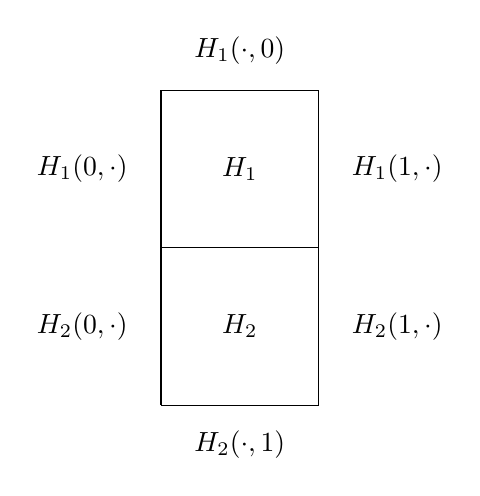
\begin{tikzpicture}[scale=0.5]
  \draw
    (0,0)
    --
    (4,0)
    --
    (4,4)
    --
    (0,4)
    --
    (0,0);
  \draw
    (0,4)
    --
    (0,8)
    --
    (4,8)
    --
    (4,4);
  \draw
    (2,2)
    --
    (2,2) node[fill=white] {$H_{2}$};
  \draw
    (2,6)
    --
    (2,6) node[fill=white] {$H_{1}$};
  \draw
    (2,-1)
    --
    (2,-1) node[fill=white] {$H_{2}(\cdot,1)$};
  \draw
    (2,9)
    --
    (2,9) node[fill=white] {$H_{1}(\cdot,0)$};
  \draw
    (-2,2)
    --
    (-2,2) node[fill=white] {$H_{2}(0,\cdot)$};
  \draw
    (-2,6)
    --
    (-2,6) node[fill=white] {$H_{1}(0,\cdot)$};
  \draw
    (6,2)
    --
    (6,2) node[fill=white] {$H_{2}(1,\cdot)$};
  \draw
    (6,6)
    --
    (6,6) node[fill=white] {$H_{1}(1,\cdot)$};
\end{tikzpicture}
\]
And if the homotopies were $2$-paths from $H_{1}(\cdot,0)$ to $H_{1}(\cdot,1)$ and from $H_{2}(\cdot,0)$ to $H_{2}(\cdot,1)$, respectively, then we would draw
\[
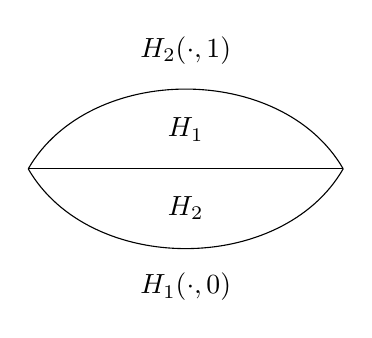
\begin{tikzpicture}[scale=1]
  \draw
    (0,2)
    to[bend left=60]
    (4,2);
  \draw
    (0,2)
    --
    (4,2);
  \draw
    (0,2)
    to[bend right=60]
    (4,2);
  \draw
    (2,2.5)
    --
    (2,2.5) node[fill=white] {$H_{1}$};
  \draw
    (2,1.5)
    --
    (2,1.5) node[fill=white] {$H_{2}$};
  \draw
    (2,0.5)
    --
    (2,0.5) node[fill=white] {$H_{1}(\cdot,0)$};
  \draw
    (2,3.5)
    --
    (2,3.5) node[fill=white] {$H_{2}(\cdot,1)$};
\end{tikzpicture}
\]
And this clearly makes sense for $n > 2$. This composition has the following properties:
\begin{enumerate}
\item[(a)]
It is associative up to homotopy. This is to say that composing $n$-paths is only associative up to an $n+1$-path.
\item[(b)]
Composing an $n$-path with the constant $n$-path (a constant $n$-path is one which is independent of its last coordinate) on the left or on the right reproduces the $n$-path up to homotopy suggesting that the constant $n$-path is an identity up to homotopy. In other words, composing an $n$-path with the constant $n$-path obeys a unital law up to an $n+1$-path.
\item[(c)]
With respect to the identity from (b) one can invert an $n$-path up to homotopy, that is, up to an $n+1$-path.
\end{enumerate}
But this kind of path composition is not the only one for $n \geq 2$. We rather have $n$ compositions for $n$-paths. For if given homotopies
\begin{align*}
  H_{1},H_{2}
  \colon
  I
  \times
  I
  &\rightarrow
  Y
\end{align*}
we can compose homotopies (up to a homotopy of homotopies) along the second coordinate if
\begin{align*}
  H_{1}(1,\cdot)
  &=
  H_{2}(0,\cdot)
\end{align*}
as illustrated by the picture
\[
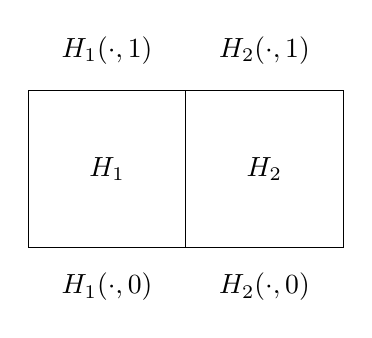
\begin{tikzpicture}[scale=0.5]
  \draw
    (0,0)
    --
    (4,0)
    --
    (4,4)
    --
    (0,4)
    --
    (0,0);
  \draw
    (4,0)
    --
    (8,0)
    --
    (8,4)
    --
    (4,4);
  \draw
    (2,2)
    --
    (2,2) node[fill=white] {$H_{1}$};
  \draw
    (6,2)
    --
    (6,2) node[fill=white] {$H_{2}$};
  \draw
    (2,-1)
    --
    (2,-1) node[fill=white] {$H_{1}(\cdot,0)$};
  \draw
    (6,-1)
    --
    (6,-1) node[fill=white] {$H_{2}(\cdot,0)$};
  \draw
    (2,5)
    --
    (2,5) node[fill=white] {$H_{1}(\cdot,1)$};
  \draw
    (6,5)
    --
    (6,5) node[fill=white] {$H_{2}(\cdot,1)$};
\end{tikzpicture}
\]
And if the homotopies were $2$-paths from $H_{1}(\cdot,0)$ to $H_{1}(\cdot,1)$ and from $H_{2}(\cdot,0)$ to $H_{2}(\cdot,1)$, respectively, then we would draw
\[
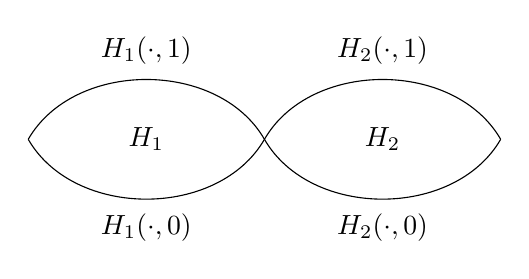
\begin{tikzpicture}[scale=0.75]
  \draw
    (0,2)
    to[bend left=60]
    (4,2);
  \draw
    (0,2)
    to[bend right=60]
    (4,2);
  \draw
    (4,2)
    to[bend left=60]
    (8,2);
  \draw
    (4,2)
    to[bend right=60]
    (8,2);
  \draw
    (2,2)
    --
    (2,2) node[fill=white] {$H_{1}$};
  \draw
    (6,2)
    --
    (6,2) node[fill=white] {$H_{2}$};
  \draw
    (2,0.5)
    --
    (2,0.5) node[fill=white] {$H_{1}(\cdot,0)$};
  \draw
    (6,0.5)
    --
    (6,0.5) node[fill=white] {$H_{2}(\cdot,0)$};
  \draw
    (2,3.5)
    --
    (2,3.5) node[fill=white] {$H_{1}(\cdot,1)$};
  \draw
    (6,3.5)
    --
    (6,3.5) node[fill=white] {$H_{2}(\cdot,1)$};
\end{tikzpicture}
\]
All this also makes sense for $n > 2$. For these compositions we again have associativity, unital laws and invertibility only up to higher paths. But this {\glqq}up to higher paths{\grqq} is not arbitrary in classical homotopy theory. Let us discuss this a bit in the case of composing $1$-paths up to $2$-paths. The point we want to address is that associativity and the identity law of $1$-path composition is up to \underline{coherent} homotopy. This is to say that there is a family $A(p_{1},p_{2},p_{3})$ of homotopies parametrized by appropriate $1$-paths $p_{1},p_{2},p_{3}$ such that given two parenthesizations of a concatenation of arbitrarily many $1$-paths it does not matter (up to homotopy) how we apply the elements of the family $\lbrace A(p_{1},p_{2},p_{3}) \rbrace$ to go from one to the other. This can be derived from the assumption that the $2$-paths
\begin{align*}
  A_{1}
  &:=
  A(p_{2} \circ p_{1},p_{3},p_{4})
  \circ
  A(p_{1},p_{2},p_{4} \circ p_{3})
\end{align*}
and
\begin{align*}
  A_{2}
  &:=
  \left(
    \mathrm{id}_{p_{4}}
    \circ^{\textrm{h}}
    A(p_{1},p_{2},p_{3})
  \right)
  \circ
  A(p_{1},p_{3} \circ p_{2},p_{4})
  \circ
  \left(
    A(p_{2},p_{3},p_{4})
    \circ^{\textrm{h}}
    \mathrm{id}_{p_{1}}
  \right)
\end{align*}
from
\begin{align*}
  \left(
    (p_{4} \circ p_{3})
    \circ
    p_{2}
  \right)
  \circ
  p_{1}
\end{align*}
to
\begin{align*}
  p_{4}
  \circ
  \left(
    p_{3}
    \circ
    (p_{2} \circ p_{1})
  \right)
\end{align*}
are homotopic, that is, the diagram
\[
\begin{tikzcd}[row sep=3.5em,column sep=0.4em]
  &
  (p_{4} \circ p_{3})
  \circ
  (p_{2} \circ p_{1})
  \arrow{dr}{A(p_{2} \circ p_{1},p_{3},p_{4})}
  &
  \\
  \left(
    (p_{4} \circ p_{3})
    \circ
    p_{2}
  \right)
  \circ
  p_{1}
  \arrow{ur}{A(p_{1},p_{2},p_{4} \circ p_{3})}
  \arrow[swap]{d}{A(p_{2},p_{3},p_{4}) \circ^{\textrm{h}} \mathrm{id}_{p_{1}}}
  &
  &
  p_{4}
  \circ
  \left(
    p_{3}
    \circ
    (p_{2} \circ p_{1})
  \right)
  \\
  \left(
    p_{4}
    \circ
    (p_{3} \circ p_{2})
  \right)
  \circ
  p_{1}
  \arrow{rr}{A(p_{1},p_{3} \circ p_{2},p_{4})}
  &
  &
  p_{4}
  \circ
  \left(
    (p_{3} \circ p_{2})
    \circ
    p_{1}
  \right)
  \arrow[swap]{u}{\mathrm{id}_{p_{4}} \circ^{\textrm{h}} A(p_{1},p_{2},p_{3})}
\end{tikzcd}
\]
commutes up to homotopy.
\begin{align*}
  A_{1}
  &\sim
  A_{2}
\end{align*}
is known as Stasheff's pentagon identity. And deriving associativity up to coherent homotopy from Stasheff's pentagon identity can be considered a so-called {\glqq}coherence theorem{\grqq} for the {\glqq}coherence condition{\grqq} $A_{1} \sim A_{2}$. In a similar vein the identity law is treated to obtain a coherence theorem for a coherence condition in this case, too. To this end let $\mathrm{const}_{y}$ denote the $1$-path constant at $y \in Y$. Moreover note that if additionally to the family $A(p_{1},p_{2},p_{3})$ we have for all $1$-paths $p_{1}$ homotopies $R(p_{1})$ from $p_{1} \circ \mathrm{const}_{p_{1}(0)}$ to $p_{1}$ and
$L(p_{1})$ from $\mathrm{const}_{p_{1}(1)} \circ p_{1}$ to $p_{1}$, respectively, then we get that the homotopy
\begin{align*}
  R(p_{2})
  \circ^{\textrm{h}}
  \mathrm{id}_{p_{1}}
\end{align*}
is homotopic to the homotopy
\begin{align*}
  \left(
    \mathrm{id}_{p_{2}}
    \circ^{\textrm{h}}
    L(p_{1})
  \right)
  \circ
  A(p_{1},\mathrm{const}_{p_{1}(1)},p_{2})
\end{align*}
both from
\begin{align*}
  \left(
    p_{2}
    \circ
    \mathrm{const}_{p_{1}(1)}
  \right)
  \circ
  p_{1}
\end{align*}
to
\begin{align*}
  p_{2}
  \circ
  p_{1}
\end{align*}
This means the diagram
\[
\begin{tikzcd}[sep=large]
  \left(
    p_{2}
    \circ
    \mathrm{const}_{p_{1}(1)}
  \right)
  \circ
  p_{1}
  \arrow{rr}{A(p_{1},\mathrm{const}_{p_{1}(1)},p_{2})}
  \arrow[swap]{dr}{R(p_{2}) \circ^{\textrm{h}} \mathrm{id}_{p_{1}}}
  &
  &
  p_{2}
  \circ
  \left(
    \mathrm{const}_{p_{1}(1)}
    \circ
    p_{1}
  \right)
  \arrow{dl}{\mathrm{id}_{p_{2}} \circ^{\textrm{h}} L(p_{1})}
  \\
  &
  p_{2}
  \circ
  p_{1}
  &
\end{tikzcd}
\]
commutes up to homotopy. This is known as triangle identity. And deriving the unit laws up to coherent homotopy from the triangle identity can be considered a so-called {\glqq}coherence theorem{\grqq} for the {\glqq}coherence condition{\grqq} imposed by the triangle identity. In both cases the homotopies making the diagrams {\glqq}commute{\grqq} satisfy their own coherence conditions and so on. \cite{69cbf29c} seems to be a good source to gain insight into this process.
\item[$\bullet$]
Let $n$ be a natural number and let $(S^{n},s^{n})$ denote a pointed $n$-sphere (as a pointed topological space). Let further $(Y,y)$ denote a pointed space. Then a base-point preserving continuous function $l \colon S^{n} \rightarrow Y$ is called an \textbf{$n$-loop (in $Y$)}. This can be regarded as an $n$-path with starting point and terminus the same point of the space regarded as degenerate $n-1$-path (identity of identity of identity of \ldots). So the same reasoning about composition of $n$-paths applies. But then, by dividing out homotopy from composition of $n$-loops, the $n$-loops for fixed $n$ should form a group. And, indeed,
\begin{align*}
  \pi_{n}(Y,y)
  &:=
  \langle
    S^{n},
    Y
  \rangle
\end{align*}
is called the \textbf{$n$-th homotpy group (of $(Y,y)$)} while the first homotopy group is often called \textbf{fundamental group (of $(Y,y)$)}. For $n \geq 1$, $\pi_{n}$ is actually a functor from $\mathbf{Top}_{\ast}$ to $\mathbf{Grp}$ (and for $n \geq 2$ even to $\mathbf{Ab}$). Note that $\pi_{0}(Y)$ is not actually a group.
\item[$\bullet$]
We can now define categories $\mathbf{HTop}$ and $\mathbf{HTop}_{\ast}$ by
\begin{align*}
  \mathrm{ob}_{\mathbf{HTop}}
  &:=
  \mathrm{ob}_{\mathbf{Top}}
  \\
  \mathrm{mor}_{\mathbf{HTop}}(Y_{1},Y_{2})
  &:=
  [Y_{1},Y_{2}]
\end{align*}
in the unpointed case and
\begin{align*}
  \mathrm{ob}_{\mathbf{HTop}_{\ast}}
  &:=
  \mathrm{ob}_{\mathbf{Top}_{\ast}}
  \\
  \mathrm{mor}_{\mathbf{HTop}_{\ast}}(Y_{1},Y_{2})
  &:=
  \langle
    Y_{1},
    Y_{2}
  \rangle
\end{align*}
in the pointed case. These become categories by noting that we can compose homotopies (relative $A_{1} \subset Y_{1}$) horizontally (up to higher homotopy) as sketched above. $\mathbf{HTop}$ is called \textbf{naive homotopy category (of $\mathbf{Top}$)} while $\mathbf{HTop}_{\ast}$ is called \textbf{(pointed) naive homotopy category (of $\mathbf{Top}_{\ast}$)}. Note that for subcategories $\mathbf{Top}^{\textrm{Name}}$ of $\mathbf{Top}$ and $\mathbf{Top}_{\ast}^{\textrm{Name}}$ of $\mathbf{Top}_{\ast}$ we get according subcategories of the naive homotopy categories which we denote $\mathbf{HTop}^{\textrm{Name}}$ and $\mathbf{HTop}_{\ast}^{\textrm{Name}}$, respectively. $\mathbf{HTop}^{\textrm{Name}}$ is called \textbf{naive homotopy category (of $\mathbf{Top}^{\mathrm{Name}}$)} while $\mathbf{HTop}_{\ast}^{\textrm{Name}}$ is called \textbf{(pointed) naive homotopy category (of $\mathbf{Top}_{\ast}^{\mathrm{Name}}$)}. The functors $\pi_{n}$ can now be made into functors on $\mathbf{HTop}_{\ast}$.
\item[$\bullet$]
Representatives of isomorphisms of $\mathbf{HTop}$ are called \textbf{strong homotopy equivalences}. Assume a strong homotopy equivalence $f \colon Y_{1} \rightarrow Y_{2}$. Then due to theorem \ref{thm:catiso} we have that
\begin{align*}
  \pi_{n}([f])
  &=
  \pi_{n}(f)
\end{align*}
is an isomorphism. This gives rise to an idea of a weaker notion of homotopy equivalence. At this point note that {\glqq}strong{\grqq} is not really standard in traditional literature. But we will explain in a moment why we opted for it. A morphism $f \colon Y_{1} \rightarrow Y_{2}$ of $\mathbf{Top}$ or $\mathbf{Top}_{\ast}$ is called \textbf{(weak) homotopy equivalence (of $Y_{1}$ and $Y_{2}$)} if $\pi_{n}(f)$ is an isomorphism for all $n \in \mathbb{N}$. Homotopy equivalences are not strong homotopy equivalences in general but they are for CW complexes. The latter fact is known as Whitehead's theorem.
\item[$\bullet$]
If there is an $n_{0} \in \mathbb{N}$ such that for all $n > n_{0}$ the homotopy groups $\pi_{n}(Y,y)$ consist of a single element we say that $Y$ is a \textbf {(topological) homotopy $n_{0}$-type}, else we say that $Y$ is a \textbf{(topological) homotopy $\infty$-type}. Note that this is not always standard terminology. We discuss this in a moment.
\end{enumerate}
This review of classical homotopy theory has a few implications which are the topic of the rest of this subsection.
\\
We paid attention chiefly to $n$-paths. You might guess why: the $1$-paths in a topological space $Y$ behave as the morphisms in a groupoid if we factor out homotopies. Formally, for a topological space $Y$ define a groupoid $\Pi_{1}(Y)$ with objects just the points of the space $Y$ and morphisms from a point $y_{1}$ to a point $y_{2}$ of $Y$ just the homotopy classes of paths from $y_{1}$ to $y_{2}$ by the (C3) trick from remark \ref{rem:c3trick}. Clearly the morphisms from $y \in Y$ to itself are the same as the group $\pi_{1}(Y,y) = \langle S^{1},Y \rangle$. $\Pi_{1}(Y)$ is the literally fundamental example of groupoids and is therefore called \textbf{fundamental groupoid (of $Y$)}. But we can see even more. Namely, $2$-paths behave just as we wished the $2$-morphisms of a weak $2$-groupoid to behave. But we now have a real idea for conditions when the notion of associativity and unit law is {\glqq}coherent{\grqq}: We weaken as proposed before the classical homotopy theory discussion but motivated from classical homotopy theory we also demand
\begin{enumerate}
\item[(1)]
\begin{align*}
  \mathsf{A}_{1}
  &=
  \mathsf{A}_{2}
\end{align*}
\item[(2)]
\begin{align*}
  \mathsf{R}(f_{23})
  \circ^{\textrm{h}}
  \mathrm{id}_{f_{12}}
  &=
  \left(
    \mathrm{id}_{f_{23}}
    \circ^{\textrm{h}}
    \mathsf{L}(f_{12})
  \right)
  \circ
  \mathsf{A}(f_{12},\mathsf{id}_{X_{2}},f_{23})
\end{align*}
\end{enumerate}
If one can then prove an appropriate coherence theorem to interpret these as coherence conditions - and one can as Mac Lane has shown - then we are done. So let us formally define weak $2$-category\footnote{for historical reasons this is sometimes called bicategory}. A set ${}_{2}\mathbf{C}$ is a \textbf{(weak) $2$-category} if it is a $3$-tuple consisting of a set ${}_{0}\mathrm{mor}_{{}_{2}\mathbf{C}}$, for all $X_{1},X_{2} \in {}_{0}\mathrm{mor}_{_{2}\mathbf{C}}$ a category
\begin{align*}
  \left(
    {}_{1}\mathrm{mor}_{{}_{2}\mathbf{C}}(X_{1},X_{2}),
    {}_{2}\mathrm{mor}_{{}_{2}\mathbf{C}}(X_{1},X_{2},\cdot,\cdot),
    \circ_{(X_{1},X_{2})}^{\textrm{v}}
  \right)
  &:=
  {}_{1}\mathbf{mor}_{{}_{2}\mathbf{C}}(X_{1},X_{2})
\end{align*}
and for all $X_{1},X_{2},X_{3} \in {}_{0}\mathrm{mor}_{{}_{2}\mathbf{C}}$ a functor\footnote{if you really want to understand this you have to jump to subsection \ref{sec:prodcat} about product categories right at the beginning but you can also ignore it because it is not really the point for what follows beyond this definition}
\begin{align*}
  \circ^{\textrm{h}}
  \doteq
  \circ^{\textrm{h}}(X_{1},X_{2},X_{3})
  \doteq
  \circ_{{}_{2}{\mathbf{C}}}^{\textrm{h}}(X_{1},X_{2},X_{3})
  \colon
  {}_{1}\mathbf{mor}_{{}_{2}\mathbf{C}}(X_{1},X_{2})
  \times
  {}_{1}\mathbf{mor}_{{}_{2}\mathbf{C}}(X_{2},X_{3})
  &\rightarrow
  {}_{1}\mathbf{mor}_{{}_{2}\mathbf{C}}(X_{1},X_{3})
\end{align*}
such that
\begin{enumerate}
\item[(${}_{2}$C0)]
The $3$-tuple\footnote{note that a functor is a $4$-tuple and projection to the third coordinate is the object part}
\begin{align*}
  \left(
    {}_{0}\mathrm{mor}_{{}_{2}\mathbf{C}},
    {}_{1}\mathrm{mor}_{{}_{2}\mathbf{C}},
    \circ_{\mathbf{C}}
  \right)
\end{align*}
with
\begin{align*}
  \circ_{\mathbf{C}}
  &:=
  \circ^{1}
  \left(
    \circ_{{}_{2}\mathbf{C}}^{\textrm{h}},
    \mathrm{pr}_{3}
  \right)
\end{align*}
is such that
\begin{enumerate}
\item[(WC1)]
for all $X_{1},X_{2},X_{3},X_{4}$ there is a natural isomorphism
\begin{align*}
  \mathsf{A}
  &\doteq
  \mathsf{A}
  \left(
    X_{1},
    X_{2},
    X_{3},
    X_{4}
  \right)
\end{align*}
from
\begin{align*}
  \left(
    \cdot
    \circ
    \cdot
  \right)
  \circ
  \cdot
  &\doteq
  \circ^{\textrm{h}}(X_{1},X_{2},X_{4})
  \left(
    \cdot,
    \circ^{\textrm{h}}
    (X_{2},X_{3},X_{4})
    (\cdot,\cdot)
  \right)
\end{align*}
to
\begin{align*}
  \cdot
  \circ
  \left(
    \cdot
    \circ
    \cdot
  \right)
  &\doteq
  \circ^{\textrm{h}}
  (X_{1},X_{3},X_{4})
  \left(
    \circ^{\textrm{h}}
    (X_{1},X_{2},X_{3})
    (\cdot,\cdot),
    \cdot
  \right)
\end{align*}
making for all $f_{12},f_{23},f_{34},f_{45}$ the diagram
\[
\begin{tikzcd}[row sep=3.5em,column sep=0.4em]
  &
  (f_{45} \circ f_{34})
  \circ
  (f_{23} \circ f_{12})
  \arrow{dr}{\mathsf{A}(f_{23} \circ f_{12},f_{34},f_{45})}
  &
  \\
  \left(
    (f_{45} \circ f_{34})
    \circ
    f_{23}
  \right)
  \circ
  f_{12}
  \arrow{ur}{\mathsf{A}(f_{12},f_{23},f_{45} \circ f_{34})}
  \arrow[swap]{d}{\mathsf{A}(f_{23},f_{34},f_{45}) \circ^{\textrm{h}} \mathrm{id}_{f_{12}}}
  &
  &
  f_{45}
  \circ
  \left(
    f_{34}
    \circ
    (f_{23} \circ f_{12})
  \right)
  \\
  \left(
    f_{45}
    \circ
    (f_{34} \circ f_{23})
  \right)
  \circ
  f_{12}
  \arrow{rr}{\mathsf{A}(f_{12},f_{34} \circ f_{23},f_{45})}
  &
  &
  f_{45}
  \circ
  \left(
    (f_{34} \circ f_{23})
    \circ
    f_{12}
  \right)
  \arrow[swap]{u}{\mathrm{id}_{f_{45}} \circ^{\textrm{h}} \mathsf{A}(f_{12},f_{23},f_{34})}
\end{tikzcd}
\]
commute
\item[(WC2)]
for each $X_{1} \in \mathrm{ob}_{\mathbf{C}}$ there is an element
\begin{align*}
  \mathrm{id}_{X_{1}}
  &\in
  \mathrm{mor}_{\mathbf{C}}(X_{1},X_{1})
\end{align*}
and natural isomorphisms
\begin{align*}
  \mathsf{R}
  \doteq
  \mathsf{R}(X_{1})
  \colon
  \circ^{\textrm{h}}(\mathrm{id}_{X_{1}},\cdot)
  &\Rightarrow
  \mathrm{id}_{{}_{1}\mathbf{mor}_{{}_{2}}\mathbf{C}(X_{1},X_{2})}
  \\
  \mathsf{L}
  \doteq
  \mathsf{L}(X_{1})
  \colon
  \circ^{\textrm{h}}(\cdot,\mathrm{id}_{X_{2}})
  &\Rightarrow
  \mathrm{id}_{{}_{1}\mathbf{mor}_{{}_{2}}\mathbf{C}(X_{1},X_{2})}
\end{align*}
making for all $f_{12},f_{23}$ the diagram
\[
\begin{tikzcd}[sep=large]
  \left(
    f_{23}
    \circ
    \mathrm{id}_{X_{2}}
  \right)
  \circ
  f_{12}
  \arrow{rr}{\mathsf{A}(f_{12},\mathrm{id}_{X_{2}},f_{23})}
  \arrow[swap]{dr}{\mathsf{R}(f_{23}) \circ^{\textrm{h}} \mathrm{id}_{f_{12}}}
  &
  &
  f_{23}
  \circ
  \left(
    \mathrm{id}_{X_{2}}
    \circ
    f_{12}
  \right)
  \arrow{dl}{\mathrm{id}_{f_{23}} \circ^{\textrm{h}} \mathsf{L}(f_{12})}
  \\
  &
  f_{23}
  \circ
  f_{12}
  &
\end{tikzcd}
\]
commute
\item[(WC3)]
for all
\begin{align*}
  (X_{1},X_{2}),(X_{3},X_{4})
  &\in
  \mathrm{ob}_{\mathbf{C}}
  \times
  \mathrm{ob}_{\mathbf{C}}
\end{align*}
satisfying
\begin{align*}
  (X_{1},X_{2})
  &\neq
  (X_{3},X_{4})
\end{align*}
the the formula
\begin{align*}
  \mathrm{mor}_{\mathbf{C}}(X_{1},X_{2})
  \cap
  \mathrm{mor}_{\mathbf{C}}(X_{3},X_{4})
  &=
  \emptyset
\end{align*}
holds\footnote{this last property is a peculiarity of materlial set theories such as TG if we want the category definition to be exactly the same as the usual first order theory of category theory}.
\end{enumerate}
\item[(${}_{2}$C1)]
for all $X_{1},X_{2},X_{3},X_{4} \in {}_{0}\mathrm{mor}_{{}_{2}\mathbf{C}}$, for all
\begin{align*}
  f_{12},f_{12}^{\backprime}
  &\in
  {}_{1}\mathrm{mor}_{{}_{2}\mathbf{C}}(X_{1},X_{2})
  \\
  f_{23},f_{23}^{\backprime}
  &\in
  {}_{1}\mathrm{mor}_{{}_{2}\mathbf{C}}(X_{2},X_{3})
  \\
  f_{34},f_{34}^{\backprime}
  &\in
  {}_{1}\mathrm{mor}_{{}_{2}\mathbf{C}}(X_{3},X_{4})
\end{align*}
and for all
\begin{align*}
  {}_{2}f_{\alpha}
  &\in
  {}_{2}\mathrm{mor}_{{}_{2}\mathbf{C}}(X_{1},X_{2},f_{12},f_{12}^{\backprime})
  \\
  {}_{2}f_{\beta}
  &\in
  {}_{2}\mathrm{mor}_{{}_{2}\mathbf{C}}(X_{2},X_{3},f_{23},f_{23}^{\backprime})
  \\
  {}_{2}f_{\gamma}
  &\in
  {}_{2}\mathrm{mor}_{{}_{2}\mathbf{C}}(X_{3},X_{4},f_{34},f_{34}^{\backprime})
\end{align*}
the term
\begin{align*}
  \circ_{{}_{2}\mathbf{C}}^{\textrm{h}}
  (X_{1},X_{2},X_{4})
  \left(
    {}_{2}f_{\alpha},
    \circ_{{}_{2}\mathbf{C}}^{\textrm{h}}
    (X_{2},X_{3},X_{4})
    ({}_{2}f_{\beta},{}_{2}f_{\gamma})
  \right)
\end{align*}
equals the term
\begin{align*}
  \circ_{{}_{2}\mathbf{C}}^{\textrm{h}}
  (X_{1},X_{3},X_{4})
  \left(
    \circ_{{}_{2}\mathbf{C}}^{\textrm{h}}
    (X_{1},X_{2},X_{3})
    ({}_{2}f_{\alpha},{}_{2}f_{\beta}),
    {}_{2}f_{\gamma}
  \right)
\end{align*}
\item[(${}_{2}$C2)]
for each $X_{1} \in {}_{0}\mathrm{mor}_{{}_{2}\mathbf{C}}$ the identity $\mathrm{id}_{\mathrm{id}_{X_{1}}}$ of the identity $\mathrm{id}_{X_{1}}$ of $X_{1}$ (the former w.r.t. ${}_{1}\mathbf{mor}_{{}_{2}\mathbf{C}}(X_{1},X_{2})$, the latter w.r.t. the category from property (${}_{2}$C0)) satisfies for all
\begin{align*}
  f_{12},f_{12}^{\backprime}
  &\in
  {}_{1}\mathrm{mor}_{{}_{2}\mathbf{C}}(X_{1},X_{2})
  \\
  f_{21},f_{21}^{\backprime}
  &\in
  {}_{1}\mathrm{mor}_{{}_{2}\mathbf{C}}(X_{2},X_{1})
\end{align*}
and for all
\begin{align*}
  {}_{2}f_{\alpha}
  &\in
  {}_{2}\mathrm{mor}_{{}_{2}\mathbf{C}}(X_{1},X_{2},f_{12},f_{12}^{\backprime})
  \\
  {}_{2}f_{\beta}
  &\in
  {}_{2}\mathrm{mor}_{{}_{2}\mathbf{C}}(X_{2},X_{1},f_{21},f_{21}^{\backprime})
\end{align*}
with $X_{2} \in {}_{0}\mathrm{mor}_{{}_{2}\mathbf{C}}$ both
\begin{align*}
  \circ_{{}_{2}\mathbf{C}}^{\textrm{h}}
  (X_{1},X_{1},X_{2})
  (\mathrm{id}_{\mathrm{id}_{X_{1}}},{}_{2}f_{\alpha})
  &=
  {}_{2}f_{\alpha}
\end{align*}
and
\begin{align*}
  \circ_{{}_{2}\mathbf{C}}^{\textrm{h}}
  (X_{2},X_{1},X_{1})
  ({}_{2}f_{\beta},\mathrm{id}_{\mathrm{id}_{X_{1}}})
  &=
  {}_{2}f_{\beta}
\end{align*}
\item[(${}_{2}$C3)]
for all $X_{1},X_{2},X_{3},X_{4} \in {}_{0}\mathrm{mor}_{{}_{2}\mathbf{C}}$, for all
\begin{align*}
  f_{12},f_{12}^{\backprime}
  &\in
  {}_{1}\mathrm{mor}_{{}_{2}\mathbf{C}}(X_{1},X_{2})
  \\
  f_{34},f_{34}^{\backprime}
  &\in
  {}_{1}\mathrm{mor}_{{}_{2}\mathbf{C}}(X_{3},X_{4})
\end{align*}
such that
\begin{align*}
  (X_{1},X_{2},f_{12},f_{12}^{\backprime})
  &\neq
  (X_{3},X_{4},f_{34},f_{34}^{\backprime})
\end{align*}
the formula
\begin{align*}
  {}_{2}\mathrm{mor}_{{}_{2}\mathbf{C}}(X_{1},X_{2}f_{12},f_{12}^{\backprime})
  \cap
  {}_{2}\mathrm{mor}_{{}_{2}\mathbf{C}}(X_{3},X_{4}f_{34},f_{34}^{\backprime})
  &=
  \emptyset
\end{align*}
holds\footnote{this property is again an annoying technicality of material set theories}
\end{enumerate}
You see right. Only property (${}_{2}$C0) differs from the definition of a strict category in that we do not demand category anymore but only category with associativity and unit law up to coherent isomorphism. This way can be gone further to obtain even higher categories since we have taken only homotopy up to dimension $2$ into account yet. This is a really artificial restriction and we should actually take all $n$-paths into account to obtain the fundamental $\infty$-groupoid of a space $Y$ as an informal weak $\infty$-groupoid. Then in a similar manner we can try to get ideas for coherence conditions to yield a definition of weak higher categories (and hence groupoids) if we can show the coherence theorems for these coherence conditions. However, this is still a terribly complicated process and once more homotopy theory may help by the following observation. Having the definition of weak $2$-groupoids as above then if $Y$ is a
\begin{enumerate}
\item[(0)]
topological homotopy $0$-type, the fundamental $2$-groupoid of $Y$ has as $1$-morphisms only identity $1$-morphisms (up to coherent homotopy) and as $2$-morphisms only identity $2$-morphisms. Hence it is actually just a set of $0$-morphisms - a set, a discrete $2$-groupoid or say $0$-groupoid. And of course, any $0$-groupoid can be regarded as fundamental $2$-groupoid for some topological homotopy $0$-type.
\item[(1)]
topological homotopy $1$-type, the fundamental $2$-groupoid of $Y$ has as $2$-morphisms only identity $2$-morphisms. Hence it is actually just a common groupoid. And of course, any $1$-groupoid can be regarded as fundamental groupoid for some topological homotopy $1$-type.
\item[(2)]
topological homotopy $2$-type, the fundamental $2$-groupoid $Y$ is some $2$-groupoid. And of course, any $2$-groupoid can be regarded as fundamental $2$-groupoid for some topological homotopy $2$-type.
\end{enumerate}
Hence the topological spaces up to weak homotopy equivalence correspond to weak $2$-groupoids. Is this generalizable to higher dimensions? This is what Grothendieck famously conjectured: The Grothendieck hypothesis.
\\
\begin{prp}[Grothendieck]
\label{prp:groth}
(Weak) $n$-groupoids are equivalent to topological homotopy $n$-types for $n \in \mathbb{N} \cup \lbrace \infty \rbrace$.
\end{prp}
\begin{prf}
That depends a bit as we will now see.
\\
\phantom{proven}
\hfill
$\square$
\end{prf}
The truth of the Grothendieck hypothesis \ref{prp:groth} depends on the definition of higher groupoids. If we define groupoids as suggested then it is trivially true. However, proceeding from this definition of higher groupoids makes it hard to define higher categories since we have to prove coherence theorems for all the coherence conditions in all dimensions to show this definition of higher categories to be sensible. On the other hand it is quite easy to get higher groupoids from higher categories. This suggests to use the Grothendieck hypothesis \ref{prp:groth} indirectly as consistency test for a definition of higher categories to check that the definition is coherent in the sense that even if the coherence conditions do not appear in the higher category definition - and that is what we actually want - they are still present. This is to say that the Grothendieck hypothesis \ref{prp:groth} as theorem is a litmus test for a sensible definition of higher categories with weak associatively composable higher directed paths obeying a weak identity law. This is how higher category theory is done nowadays. We will provide some literature on the topic in section \ref{sec:metaidea} where we elaborate on it a bit further.
\\
A further implication of the review of classical homotopy theory is the impression that homotopy theory is more about paths than homotopies between functions. Of course, you can object now that, by definition, paths are actually homotopies in classical homotopy theory. But note that we could fully capture the behavior of the $n$-paths we have in mind by $\infty$-groupoids when we demand the Grothendieck hypothesis \ref{prp:groth}. The $n$-paths are then {\glqq}synthetic{\grqq} and hence have a built-in continuity (contrary to the model of paths as certain continuous\footnote{in the sense of topology} functions). The {\glqq}continuity{\grqq} is then trivially the intuitively correct one for paths which are characterized by higher groupoid theory (not interpreted in a set theory but rather as formal theory). This is in analogy to how the elements of a set are trivially what we want elements of a collection to be. So we cannot get problems regarding continuity as in topology described in example \ref{exa:topology} (where the problems might be inherited from those of the notion of nearness). Moreover note that homotopies in classical homotopy theory actually behave in the same way as paths in an $\infty$-groupoid:
\begin{enumerate}
\item[(1)]
they can be composed associatively up to coherent homotopy
\item[(2)]
there is an identity law for a constant homotopy up to coherent homotopy
\item[(3)]
homotopies are invertible up to coherent homotopy
\end{enumerate}
Additionally, homotopy between functions is by the very idea a way to go from a function to another without really changing its continuity structure. It is essentially still the same function w.r.t. to continuity. Further, being homotopic as equivalence relation further emphasizes that being homotopic is the structural equality of continuous functions. In other words, homotopy is isomorphism for contiuous functions. This is perfectly reflected by the categories $\mathbf{HTop}$ and $\mathbf{HTop}_{\ast}$, respectively. And so we cannot help to think of homotopies as $1$-paths in a groupoid with objects some continuous functions. We can even sort of see the path aspect of homotopies in classical homotopy theory. To this end note that a homotopy $H$ from $f$ to $f^{\backprime}$ defines functions
\begin{align*}
  p_{H}
  \colon
  I
  &\rightarrow
  \mathrm{mor}_{\mathbf{Top}}(Y_{1},Y_{2})
  \\
  t
  &\mapsto
  H(\cdot,t)
  \\
  h
  \colon
  Y_{1}
  &\rightarrow
  \mathrm{mor}_{\mathbf{Top}}(I,Y_{2})
  \\
  y_{1}
  &\mapsto
  H(y_{1},\cdot)
\end{align*}
So $p_{H}$ suggests to consider a homotopy as a path in $\mathrm{mor}_{\mathbf{Top}}(Y_{1},Y_{2})$ while $h$ suggests to consider it a family of paths in $Y_{2}$ indexed by $Y_{1}$. Both ideas have the problem that it is not clear how to reasonably topologize $\mathrm{mor}_{\mathbf{Top}}(Y_{1},Y_{2})$ and $\mathrm{mor}_{\mathbf{Top}}(I,Y_{2})$ to make both $p_{H}$ and $h$ equivalent to $H$. This is to say that it is not clear how to define when two continuous functions are near each other. This is a common problem in different fields of mathematics. Anyways, it should intuitively hold that $p_{H}$ and $h$ are equivalent to $H$. This is even desirable in classical homotopy theory since there are some inconveniences\footnote{e.g. w.r.t. fiber and cofiber sequences} if it does not hold. This is why one usually restricts to a convenient category of topological spaces for the purpose of classical homotopy theory. We will say what that means in subsection \ref{sec:adjoint}. Anyways, what this tells us about classical homotopy theory is that it is more about $n$-paths than homotopies between continuous functions. This may seem odd to you if you are used to traditional books on algebraic topology and you might object that it is somewhat arbitrary to require homotopies to be equivalent to $p_{H}$ and $h$. But note that the only thing that fails in general is continuity in the sense of topology as described in example \ref{exa:topology}. But there we argued that continuity in that sense does not perfectly match the human idea of continuity. But for the purpose of paths we are interested in an intuitive continuity of these and hence $\mathbf{Top}$ cannot be the ideal setting. Though it is known to be a good approximation of the intuitive idea - at least when restricted to spaces with good separation properties. In this context it is interesting that the objects of the usual convenient category\footnote{so-called compactly generated spaces} are at least Fr\'{e}chet spaces, that is, fulfill the separation axiom $T_{1}$. Now the homotopy as path (or say structural equality) thinking has a consequence for what we consider a topological homotopy type. Our definition of those is in contrast to the original idea that topological spaces have the same homotopy type if and only if they are strongly homotopy equivalent. But in the light of higher category theory this is too strong. Just look at $\mathbf{Top}$. $f \colon Y_{1} \rightarrow Y_{2}$ is an isomorphism in $\mathbf{Top}$ if there is a morphism $f^{-1} \colon Y_{2} \rightarrow Y_{1}$ in $\mathbf{Top}$ such that
\begin{align*}
  f^{-1}
  \circ
  f
  &=
  \mathrm{id}_{Y_{1}}
  \\
  f
  \circ
  f^{-1}
  &=
  \mathrm{id}_{Y_{2}}
\end{align*}
A strong homotopy equivalence is then just weakening these equations to homotopies. This is to say that strong homotopy equivalence is isomorphism in $\mathbf{Top}$ (hypothetically) regarded as weak $2$-category with $2$-morphisms the homotopies (and hence all $2$-morphisms invertible). But why should we not take homotopies between homotopies into account and weaken to a $3$-categorical setting (if we have one)? This would be like stop counting at some arbitrarily chosen number. While this seems a philosophically legit stance\footnote{ultrafinitism} this thinking is rejected by most mathematicians. So if one does not explicitly want to examine topological spaces as the things they are but rather wants to examine their homotopy in our $n$-path sense with a notion of continuity as intuitive as possible then the homotopy types defined here are what one is interested in. In particular, if you are interested in physics our notion of homotopy types seems to matter more in the light of \cite{a565d200}. There, to model spacetime one uses homotopy types which are smooth in a precise sense instead of the usual manifolds which rest at topological spaces to capture nearness. \cite{a565d200} seems kind of successful to us and the purpose of these notes is among other things a soft first step to understand what is done there. But now back to the notion equality. The above motivates some more thoughts about {\glqq}being same{\grqq} in $\mathbf{Cat}$. Two objects $X_{1}$ and $X_{2}$ of a $2$-category are considered the same if they are isomorphic up to coherent isomorphism, that is, if there is a $1$-morphism from $X_{1}$ to $X_{2}$ which is reversible up to isomorphism. Written down formally this looks like the formula of strong homotopy equivalence of spaces $Y_{1}$ and $Y_{2}$. Though $\mathbf{Cat}$ is considered a strict $2$-category it makes sense to define a weaker notion of being the same than isomorphism, motivated from the weak $2$-category case. So $F_{\alpha\beta}$ is an \textbf{equivalence (from $\mathbf{C}_{\alpha}$ to $\mathbf{C}_{\beta}$)} if there is $F_{\beta\alpha}$ such that there exist natural isomorphisms from $F_{\beta\alpha} \circ F_{\alpha\beta}$ to $\mathrm{id}_{\mathbf{C}_{\alpha}}$ and from $F_{\alpha\beta} \circ F_{\beta\alpha}$ to $\mathrm{id}_{\mathbf{C}_{\beta}}$. $F_{\beta\alpha}$ is then called \textbf{weak inverse (of $F_{\alpha\beta}$)}. Moreover if $F_{\alpha\beta}$ is an equivalence from $\mathbf{C}_{\alpha}$ to $\mathbf{C}_{\beta}$ we say $\mathbf{C}_{\alpha},\mathbf{C}_{\beta}$ are \textbf{equivalent} and write
\begin{align*}
  \mathbf{C}_{\alpha}
  &\simeq
  \mathbf{C}_{\beta}
\end{align*}
Many properties of categories are still invariant under this weaker notion of being the same. We just have to follow the {\glqq}principle of equivalence{\grqq}. Informally, this means that we should compare objects of a category always just for isomorphism and not for equality. Or more general, equality is only appropriate for the highest morphism level whereas on the other levels we should use coherent isomorphisms. Formally, we can express this in UFP-HoTT using the already adressed univalence axiom. The basic mathematical objects of UFP-HoTT are $\infty$-groupoids. Let us roughly explain how this works. The things in the mathematical universe are types and types can have inhabitants. For $x$ inhabiting the type $X$ one usually writes $x \colon X$. There are types with inhabitants types and any type inhabits such a type. So these types are in spirit as the Grothendieck universes here. To assure the $\infty$-groupoid behavior of the types one demands that for any type $X$ and inhabitants $x_{1}$ and $x_{2}$ of $X$ there is a type $x_{1} =_{X} x_{2}$ and we have an inhabitant $\mathrm{refl}_{x} \colon x =_{X} x$ for all $x \colon X$. This can be understood as the type of paths from $x_{1}$ to $x_{2}$ (or proofs of equality of $x_{1}$ and $x_{2}$ if you like) and an identity path from $x = x$ where $\mathrm{refl}_{x}$ shall stand for reflexivity. Since the so called identity type $x_{1} =_{X} x_{2}$ is itself a type we can repeat this to get ($2$-)paths and so on. This is the essence of the $n$-path definition in classical homotopy theory. These identity types are governed by a universal property\footnote{in the sense we introduce in section \ref{sec:uni}} which is called path induction. It means that if we have a type $C(x_{1},x_{2},p)$ for each path $p \colon x_{1} =_{X} x_{2}$ in a type $X$ then suffices to show that all the $C(x,x,\mathrm{refl}_{x})$ are inhabited to conclude that all $C(x_{1},x_{2},p)$ are inhabited. This can be interpreted classically as a characterization of the free path space. This induction is in analogy to the one of natural numbers where it suffices to proof a property depending on a natural number to be true for $0$ and if it is true for some $n$ then also for $n+1$ to conlude that it is true for all natural numbers. One then wants all (higher\footnote{here also higher paths and not only inhabitants play a role}) inductive types to exist. This includes product types, sum types and function types\footnote{think about the notation $f \colon X_{1} \rightarrow X_{2}$ at this point} for example. Then univalence, which is roughly the statement that
\begin{enumerate}
\item[$\bullet$]
two inhabitants $X_{1},X_{2}$ of a universe $\mathcal{U}$ are equal in the sense $X_{1} =_{\mathcal{U}} X_{2}$ if and only if $X_{1}$ is equivalent to $X_{2}$ which means there is a function\footnote{this is actually an $\infty$-functor} from $X_{1}$ to $X_{2}$ with left and right inverse.
\end{enumerate}
assures the homotopy behaviour and the Grothendieck hypothesis \ref{prp:groth} is true. This is what makes UFP-HoTT a synthetic homotopy theory\footnote{this is to classical homotopy theory as Euclidean geometry is to analytic geometry if classical homotopy theory is understood in the homotopy type sense} and at the same time a very interesting possible foundation of mathematics since it is clear that sets are only a special case of $\infty$-groupoids - or better in this context: homotopy types. We do not want to do UFP-HoTT here too much but we will often allude to it in these notes. If you are interested in homotopy theory (as a reader interested in physics should be) then you should definitely read the really amazing HoTT book \cite{1ba1603e}. Now back to the principle of equivalence we promised being formalizable in the UFP-HoTT: Assume an $\infty$-groupoid/(homotopy) type $X$ and a property $P$ depending on objects/inhabitants/points of $X$ - this is informally\footnote{formally it would be a function from $X$ to a universe of types} a statement depending on the inhabitants of $X$ - then $P$ is called \textbf{compatible with equivalence} if for inhabitants $x_{1}$ and $x_{2}$ connected by a path of $X$ we have the statement: $P(x_{1})$ is true if and only if $P(x_{2})$ is true. Anyways this should make clear why we defined embedding as fully faithful functor. We want to adhere to the principle of equivalence which prevents us from demanding injectivity on objects but rather suggests to take injectivity up to isomorphism on objects what we automatically get from theorem \ref{thm:catiso} for embeddings. There is still another good reason to define embedding as we did. It is derived from embeddings of topological spaces and the relation of topological spaces to the {\glqq}topos of sheaves on a space{\grqq}. But we have to work a bit until we can define this at all. Overall, we recommend to read the rest of the notes before diving into higher category theory and homotopy theory where required since we develop many ideas one needs there.
\\
Last let us emphasize that homotopy theory in our $\infty$-groupoid sense is a special case of higher category theory which was already recognized by Grothendieck. We will seize that idea again in section \ref{sec:metaidea}.



\section{Duality}
\label{sec:duality}
Duality in mathematics is about two different perspectives on one and the same mathematical object. One usually has an operation of how to change the viewpoint. Applying this operation yields the dual notion of the object under consideration and doing it twice does not change anything. Thus changing the viewpoint is an involutive opertion. Now how can we change the perspective on arrows? Take a transparent page and draw an arrow on it. Then turn the page. What happens? The arrow points in the opposite direction but it is still the same arrow. Turning the page again is as if nothing has happened. So dualizing an arrow is to consider its source as target and its target as source. This is what we do in this section to see what amazing but sometimes a bit confusing things happen.
\\\\
For a category $\mathbf{C}$ we can build the category $\mathbf{C}^{\mathrm{op}}$ with objects
\begin{align*}
  \mathrm{ob}_{\mathbf{C}^{\mathrm{op}}}
  &:=
  \mathrm{ob}_{\mathbf{C}}
\end{align*}
and morphisms
\begin{align*}
  \mathrm{mor}_{\mathbf{C}^{\mathrm{op}}}(X_{1},X_{2})
  &:=
  \mathrm{mor}_{\mathbf{C}}(X_{2},X_{1})
\end{align*}
where composition is given by
\begin{align*}
  \circ_{\mathbf{C}^{\mathrm{op}}}
  (X_{1},X_{2},X_{3})
  (f_{21},f_{32})
  &:=
  \circ_{\mathbf{C}}
  (X_{3},X_{2},X_{1})
  (f_{32},f_{21})
\end{align*}
$\mathbf{C}^{\mathrm{op}}$ is then called the \textbf{opposite category (of $\mathbf{C}$)}. It is easy to verify that the opposite category is a category justifying the terminology. A category can always be seen as an opposite category. Namely as the opposite of its opposite category
\begin{align*}
  \left(
    \mathbf{C}^{\mathrm{op}}
  \right)^{\mathrm{op}}
  &=
  \mathbf{C}
\end{align*}
This reflects the duality between category and opposite category manifesting the idea of duality that both notions are two different viewpoints of the same abstract thing obtained by an involutive operation $^{\mathrm{op}}$. This is ultimately seen by the observation that a statement is true about a category if and only if it is true about the opposite category. More formally - and the following involves quite a bit of mathematical logic - let $\Sigma$ be a formula in the first-order theory of TG. A formula $\Sigma_{\mathbf{C}}^{\prime}$ is \textbf{(categorically) dual to $\Sigma$ w.r.t. $\mathbf{C}$} if $\Sigma_{\mathbf{C}}^{\prime}$ is obtained from $\Sigma$ by replacing each occurence of the formula defined by $\mathrm{mor}_{\mathbf{C}}$ by the formula defined by $\mathrm{mor}_{\mathbf{C}^{\mathrm{op}}}$ and by replacing each occurence of the formula defined by $\circ_{\mathbf{C}}$ by the formula defined by $\circ_{\mathbf{C}^{\mathrm{op}}}$. In a nutshell for the reader not that familiar with mathematical logic: simply write $\mathbf{C}^{\mathrm{op}}$ instead of $\mathbf{C}$ in the written english sentence to get the dual w.r.t. $\mathbf{C}$. Moreover since the opposite category of the opposite category of $\mathbf{C}$ is clearly $\mathbf{C}$ itself this implies that $\Sigma = (\Sigma_{\mathbf{C}}^{\prime})_{\mathbf{C}^{\mathrm{op}}}^{\prime}$. Now note that a formula is a finite sequence of first-order letters. Consequently, there can only be a finite number category variables w.r.t. which we can dualize. Hence a formula $\Sigma^{\prime}$ is said to be \textbf{(categorically) dual to $\Sigma$} if it is obtained from $\Sigma$ by dualizing w.r.t. all category variables by finite induction. In particular we get $\Sigma = (\Sigma^{\prime})^{\prime}$. As a remark for practice: dualizing is intuitively understood as reversing all arrows in the drawing of some commutative diagram but holding the sources and targets fixed. Next we should mention that definitions used here (and in general in mathematics) are english words or more general sequences of symbols standing for a certain first-order formula of TG. And so are statements. Their proofs, if existing, then are sequences of certain first-order formulas in TG. So all of them can be dualized and we speak of dual definitions, dual propositions\footnote{particularly theorems} and dual proofs respectively. The question now is if the dual proof is the proof of the dual statement. The answer is affirmative and can be stated as a meta-theorem. A meta-theorem is a statement \underline{about} the first-order theory and not in the first-order theory itself as e.g. common mathematical propositions are. To prove a meta-theorem one usually does not just use common classical logic but rather a more undisputed logic. But this meta-mathematical stuff shall not concern us here. Just note the following meta-theorem provable by an almost undisputable kind of logic.
\\
\begin{thm}[Duality Principle]
\label{thm:dp}
$\Sigma$ is a consequence in the first-order theory of TG if and only if $\Sigma_{\mathbf{C}}^{\prime}$ is a consequence in the first-order theory of TG. Hence $\Sigma$ is a consequence in the first-order theory of TG if and only if $\Sigma^{\prime}$ is a consequence in the first-order theory of TG.
\end{thm}
\begin{prf}[Sketch]
Observe that category properties (C1) and (C2) from subsection \ref{sec:cat} are true if and only if the duals to them are true. Even more, they are the same up to the category variable name. Dualizing the proof of $\Sigma$ w.r.t. $\mathbf{C}$ then yields a proof of $\Sigma_{\mathbf{C}}^{\prime}$ and vice versa since the proof just needs new variable names for $\mathbf{C}$. The second statement follows by finite induction.
\\
\phantom{proven}
\hfill
$\square$
\end{prf}
So, after all, it is justifiable to call $\mathbf{C}^{\mathrm{op}}$ the \textbf{dual of $\mathbf{C}$} as some other auhtors do. Some authors also write $\mathbf{C}^{\prime}$ instead of $\mathbf{C}^{\mathrm{op}}$. Having established this fundamental duality prinicple in category theory we want to apply it with respect to functors. First of all, we will sometimes write $f_{12}^{\mathrm{op}} := f_{21}$ for morphisms in the opposite category in accordance with our notation fixed in subsection \ref{sec:notation} of chapter \ref{chap:intro}. This is to make up for our notational convention regarding the indexing of morphisms in $\mathbf{C}$ and consequently a pure matter of convenience. Then we get
\begin{align*}
  f_{21}^{\mathrm{op}}
  \circ_{\mathbf{C}^{\mathrm{op}}}
  f_{32}^{\mathrm{op}}
  &=
  f_{12}
  \circ_{\mathbf{C}^{\mathrm{op}}}
  f_{23}
  =
  f_{23}
  \circ_{\mathbf{C}}
  f_{12}
\end{align*}
Now, if we have a functor $F \colon \mathbf{C}^{\mathrm{op}} \rightarrow \mathbf{C}_{\alpha}$ then application to compositions results in
\begin{align*}
  F(f_{23} \circ_{\mathbf{C}} f_{12})
  =
  F(f_{12})
  \circ_{\mathbf{C}_{\alpha}}
  F(f_{23})
\end{align*}
But this formula is the dual formula w.r.t. $\mathbf{C}^{\mathrm{op}}$ to the functor property (F2) regarding the functor $F$ since $\mathbf{C} = (\mathbf{C}^{\mathrm{op}})^{\mathrm{op}}$. Moreover $F_{\mathrm{mor}}$ maps
\begin{align*}
  (X_{1},X_{2})
  \in
  \mathrm{ob}_{\mathbf{C}}
  \times
  \mathrm{ob}_{\mathbf{C}}
\end{align*}
to a function
\begin{align*}
  F_{\mathrm{mor}}(X_{1},X_{2})
  \colon
  \mathrm{mor}_{\mathbf{C}}(X_{2},X_{1})
  &\rightarrow
  \mathrm{mor}_{\mathbf{C}_{\alpha}}
  (F_{\mathrm{ob}}(X_{1}),F_{\mathrm{ob}}(X_{2}))
\end{align*}
Hence functors $F \colon \mathbf{C}^{\mathrm{op}} \rightarrow \mathbf{C}_{\alpha}$ are in one-to-one correspondence to $4$-tuples consisting of $\mathbf{C}$, $\mathbf{C}_{\alpha}$, a function $F^{\mathrm{ob}} \colon \mathrm{ob}_{\mathbf{C}} \rightarrow \mathrm{ob}_{\mathbf{C}_{\alpha}}$ and a function $F^{\mathrm{mor}}$ which maps
\begin{align*}
  (X_{1},X_{2})
  &\in
  \mathrm{ob}_{\mathbf{C}}
  \times
  \mathrm{ob}_{\mathbf{C}}
\end{align*}
to a function
\begin{align*}
  F^{\mathrm{mor}}(X_{1},X_{2})
  \colon
  \mathrm{mor}_{\mathbf{C}}(X_{1},X_{2})
  \rightarrow
  \mathrm{mor}_{\mathbf{C}_{\alpha}}
  (F^{\mathrm{ob}}(X_{2}),F^{\mathrm{ob}}(X_{1}))
\end{align*}
such that
\begin{enumerate}
\item[(F1$_{\mathbf{C}}^{\prime}$)]
the formula
\begin{align*}
  F^{\mathrm{mor}}(X,X)(\mathrm{id}_{X})
  &=
  \mathrm{id}_{F^{\mathrm{ob}}(X)}
\end{align*}
holds
\item[(F2$_{\mathbf{C}}^{\prime}$)]
the formula
\begin{align*}
  F^{\mathrm{mor}}(X_{1},X_{3})(f_{23} \circ f_{12})
  &=
  F^{\mathrm{mor}}(X_{1},X_{2})(f_{12})
  \circ
  F^{\mathrm{mor}}(X_{2},X_{3})(f_{23})
\end{align*}  
holds
\end{enumerate}
$(\mathbf{C},\mathbf{C}_{\alpha},F^{\mathrm{ob}},F^{\mathrm{mor}})$ is then called \textbf{contravariant functor} following the terminology of duality in (multi-)linear algebra. We shall mention that other authors call functors covariant functors. However, we will not make use of this terminology here since in place of a contrvariant functor one can equally well regard the corresponding functor on the opposite category due to the duality principle \ref{thm:dp} avoiding case analysis. But in mathematical practice it is good to have this distinction in terminology since the opposite category is sometimes not what we consider intuitive or let us better say conventional. Just look at $\mathbf{Set}$.
\\
Actually, one can argue that the terminology {\glqq}contravariant functor{\grqq} is a bit misleading in category theory since the obvious composition of contravariant functors is a covariant functor. Hence there is no contravariant counterpart of $\mathbf{Cat}$. Moreover, a contravariant functor is not the dual notion of a covariant functor. Just a partial dual notion if you like. The dual notion of functor will follow after a few conclusive words: {\glqq}variant{\grqq} means {\glqq}to change{\grqq} as word and consequently co- and contravariant express how the functor relates the involved categories. Thus co- and contravariant in category theory is still comparable to co- and contravariant in (multi-)linear algebra, albeit not as dual notion anymore. We now come to the promised dual notion of a functor. The opposite functor. We say $F^{\mathrm{op}} \colon \mathbf{C}^{\mathrm{op}} \rightarrow \mathbf{C}_{\alpha}^{\mathrm{op}}$ is the \textbf{opposite functor (of $F \colon \mathbf{C} \rightarrow \mathbf{C}_{\alpha}$)} if the equalities
\begin{align*}
  F_{\mathrm{ob}}^{\mathrm{op}}(X)
  &=
  F_{\mathrm{ob}}(X)
  \\
  F_{\mathrm{mor}}^{\mathrm{op}}(X_{1},X_{2})(f_{12}^{\mathrm{op}})
  &=
  F_{\mathrm{mor}}(X_{2},X_{1})(f_{21})
\end{align*}
hold. In the main $F^{\mathrm{op}}$ contains the same information as $F$ because it does the same with objects and morphisms by definition. Indeed, dualizing the definition of a functor results in the definition of a functor.
\\
At the end of this subsection, we want to give an example making use of the conception of the opposite category. First of all, a functor $F$ from $\mathbf{C}^{\mathrm{op}}$ to $\mathbf{C}_{\alpha}$ is sometimes called \textbf{$\mathbf{C}_{\alpha}$-valued presheaf (on $\mathbf{C}$)}. Therefore the functor category
\begin{align*}
  \mathbf{C}_{\alpha}^{\mathbf{C}^{\mathrm{op}}}
\end{align*}
is sometimes called the \textbf{category of $\mathbf{C}_{\alpha}$-valued presheaves (on $\mathbf{C}$)}. In general mathematical practice one is mainly concerned with the special case $\mathbf{C}_{\alpha} = \mathbf{Set}$. Therefore we add some special terminology. A functor $F \colon \mathbf{C}^{\mathrm{op}} \rightarrow \mathbf{Set}$ is simply called a \textbf{presheaf (on $\mathbf{C}$)} and the functor category
\begin{align*}
  \mathbf{Set}^{\mathbf{C}^{\mathrm{op}}}
\end{align*}
is simply called the \textbf{category of presheaves (on $\mathbf{C}$)}. It is also common to use the notations $\mathrm{PSh}(\mathbf{C})$ or just $\widehat{\mathbf{C}}$ for
\begin{align*}
  \mathbf{Set}^{\mathbf{C}^{\mathrm{op}}}
\end{align*}
It is hard to explain the terminology {\grqq}presheaf{\grqq} at this point. Indeed we can not give a full explanation of terminolgy in these notes. We can just vindicate {\glqq}pre{\grqq} in section \ref{sec:uni}. For an explanation for {\glqq}sheaf{\grqq} we will later refer to some literature about sheaves in which this terminology becomes more clear. A last word on presheaves on $\mathbf{C}$ here. To define sheaf one needs a notion of covering on $\mathbf{C}$. While there are different general notions of that\footnote{keywords are Grothendieck topology and Lawvere-Tierney topology} the category $\mathbf{Open}_{Y}$ for some space $Y$ absolutely suggests itself since we know that a cover of $Y$ consists of objects in $\mathbf{Open}_{Y}$. And, in fact, presheaves on $\mathbf{Open}_{Y}$ for some space $Y$ are the most basic case one is interested in sheaf theory. We will motivate and define sheaves in section \ref{sec:uni} where this will become clearer.
\\
A heap of examples of presheaves are provided by hom-functors arising from the morphism function of a category. For this purpose we fix an arbitrary object $X_{0}$ of a category $\mathbf{C}$ and define a functor
\begin{align*}
  \mathrm{hom}_{\mathbf{C}}(X_{0},\cdot)
  \colon
  \mathbf{C}
  &\rightarrow
  \mathbf{Set}
  \\
  X
  &\mapsto
  \mathrm{mor}_{\mathbf{C}}(X_{0},X)
  \\
  f_{12}
  &\mapsto
  \left(
    f_{01}
    \mapsto
    f_{12}
    \circ
    f_{01}
  \right)
\end{align*}
$\mathrm{hom}_{\mathbf{C}}(X_{0},\cdot)$ is called \textbf{covariant hom-functor (for $X_{0}$ and $\mathbf{C}$)}. Note that
\begin{align*}
  \mathrm{hom}_{\mathbf{C}}(X_{0},f_{12})
  \in
  \mathrm{mor}_{\mathbf{Set}}
  \left(
    \mathrm{hom}_{\mathbf{C}}(X_{0},X_{1}),
    \mathrm{hom}_{\mathbf{C}}(X_{0},X_{2})
  \right)
\end{align*}
and that $\mathrm{hom}_{\mathbf{C}}(X_{0},f_{12})$ is so called post-composition with $f_{12}$. Likewise we define a functor
\begin{align*}
  \mathrm{hom}_{\mathbf{C}}(\cdot,X_{0})
  \colon
  \mathbf{C}^{\mathrm{op}}
  &\rightarrow
  \mathbf{Set}
  \\
  X
  &\mapsto
  \mathrm{mor}_{\mathbf{C}}(X,X_{0})
  \\
  f_{12}^{\mathrm{op}}
  &\mapsto
  \left(
    f_{01}^{\mathrm{op}}
    \mapsto
    f_{01}^{\mathrm{op}}
    \circ_{\mathbf{C}}
    f_{12}^{\mathrm{op}}
  \right)
\end{align*}
$\mathrm{hom}_{\mathbf{C}}(\cdot,X_{0})$ is called \textbf{contravariant hom-functor (for $X_{0}$ and $\mathbf{C}$)}. Note that
\begin{align*}
  \mathrm{hom}_{\mathbf{C}}(f_{12}^{\mathrm{op}},X_{0})
  \in
  \mathrm{mor}_{\mathbf{Set}}
  \left(
    \mathrm{hom}_{\mathbf{C}}(X_{1},X_{0}),
    \mathrm{hom}_{\mathbf{C}}(X_{2},X_{0})
  \right)
\end{align*}
and that $\mathrm{hom}_{\mathbf{C}}(f_{12}^{\mathrm{op}},X_{0})$ is so called pre-composition with $f_{12}^{\mathrm{op}}$. Since it is straightforward to show that the two hom-functors are functors we don't prove it here but rather consider the diagram
\[
\begin{tikzcd}[row sep=large,column sep=8em]
  \mathrm{hom}_{\mathbf{C}}(X_{3},X_{2})
  \arrow{r}{\mathrm{hom}_{\mathbf{C}}(f_{31}^{\mathrm{op}},X_{2})}
  \arrow[swap]{d}{\mathrm{hom}_{\mathbf{C}}(X_{3},f_{24})}
  &
  \mathrm{hom}_{\mathbf{C}}(X_{1},X_{2})
  \arrow{d}{\mathrm{hom}_{\mathbf{C}}(X_{1},f_{24})}
  \\
  \mathrm{hom}_{\mathbf{C}}(X_{3},X_{4})
  \arrow{r}{\mathrm{hom}_{\mathbf{C}}(f_{31}^{\mathrm{op}},X_{4})}
  &
  \mathrm{hom}_{\mathbf{C}}(X_{1},X_{4})
\end{tikzcd}
\]
This diagram commutes since $f_{32}$ is in both cases mapped to $f_{24} \circ f_{32} \circ f_{13}$ and we call this property \textbf{compatibility of hom} for the sake of easy reference. Last but not least, we shall mention that $\mathrm{hom}_{\mathbf{C}^{\mathrm{op}}}(\cdot,X_{0})$ is actually the same as $\mathrm{hom}_{\mathbf{C}}(X_{0},\cdot)$, that is,
\begin{align*}
  \mathrm{hom}_{\mathbf{C}^{\mathrm{op}}}(\cdot,X_{0})
  &=
  \mathrm{hom}_{\mathbf{C}}(X_{0},\cdot)
\end{align*}
since the opposite category of the opposite category of $\mathbf{C}$ is $\mathbf{C}$ itself. Of course,
\begin{align*}
  \mathrm{hom}_{\mathbf{C}}(\cdot,X_{0})
  &=
  \mathrm{hom}_{\mathbf{C}^{\mathrm{op}}}(X_{0},\cdot)
\end{align*}
is true as well due to the same argument. What we want to say is that in statements about hom-functors it always suffices to treat either the co- or contravariant case again reflecting the duality of $\mathbf{C}$ and $\mathbf{C}^{\mathrm{op}}$. So make a choice in accordance to your needs.



\section{Constructions on a Category}
\label{sec:constoncat}
This section just introduces some important basic constructions of categories that are quite useful in practice. There is not much to say about them here and not much interesting stuff happens here - at least at first glance. Yet it is still important to read the section. So don't skip it.


\subsection{Product Category}
\label{sec:prodcat}
Given categories $\mathbf{C}_{\alpha}$ and $\mathbf{C}_{\beta}$ we can form a category denoted $\mathbf{C}_{\alpha} \times \mathbf{C}_{\beta}$ with objects the ordered pairs $(X^{\alpha},X^{\beta})$ and morphisms the ordered pairs $(f_{12}^{\alpha},f_{12}^{\beta})$ where composition is defined by
\begin{align*}
  \circ_{\mathbf{C}_{\alpha} \times \mathbf{C}_{\beta}}
  \left(
    (X_{1}^{\alpha},X_{1}^{\beta}),
    (X_{2}^{\alpha},X_{2}^{\beta}),
    (X_{3}^{\alpha},X_{3}^{\beta})
  \right)
  \left(
    (f_{12}^{\alpha},f_{12}^{\beta}),
    (f_{23}^{\alpha},f_{23}^{\beta})
  \right)
  :=
  \left(
    f_{23}^{\alpha}
    \circ
    f_{12}^{\alpha},
    f_{23}^{\beta}
    \circ
    f_{12}^{\beta}
  \right)
\end{align*}
Further the identity in
\begin{align*}
  \mathrm{mor}_{\mathbf{C}_{\alpha}
  \times
  \mathbf{C}_{\beta}}
  \left(
    (X^{\alpha},X^{\beta}),
    (X^{\alpha},X^{\beta})
  \right)
\end{align*}
is given by $(\mathrm{id}_{X^{\alpha}},\mathrm{id}_{X^{\beta}})$. It is easy to check that this makes sense and is therefore left to the reader. $\mathbf{C}_{\alpha} \times \mathbf{C}_{\beta}$ is called the \textbf{product category (of $\mathbf{C}_{\alpha}$ and $\mathbf{C}_{\beta}$)}. From the above it is clear how the product category $\mathbf{C}_{\alpha} \times \mathbf{C}_{\beta} \times\mathbf{C}_{\gamma}$ of three categories is defined. In fact, even the case of finitely many categories is clear now. To introduce the behavior of functors regarding the construction of product categories we begin with an example. Given functors $F_{\alpha\gamma}$ and $F_{\beta\delta}$ one can define a functor
\begin{align*}
  F_{\alpha\gamma}
  \times
  F_{\beta\delta}
  \colon
  \mathbf{C}_{\alpha}
  \times
  \mathbf{C}_{\beta}
  &\rightarrow
  \mathbf{C}_{\gamma}
  \times
  \mathbf{C}_{\delta}
  \\
  (X^{\alpha},X^{\beta})
  &\mapsto
  (F_{\alpha\gamma}(X^{\alpha}),F_{\beta\delta}(X^{\beta}))
  \\
  (f_{12}^{\alpha},f_{12}^{\beta})
  &\mapsto
  \left(
    F_{\alpha\gamma}(f_{12}^{\alpha}),
    F_{\beta\delta}(f_{12}^{\beta})
  \right)
\end{align*}
That this is a functor is quite clear from the assumption that $F_{\alpha\gamma}$ and $F_{\beta\delta}$ are functors. In a more general setting, too, functors behave almost as nicely as one would wish on product categories $\mathbf{C}_{\alpha} \times \mathbf{C}_{\beta}$. If
\begin{align*}
  F
  \colon
  \mathbf{C}_{\alpha}
  \times
  \mathbf{C}_{\beta}
  &\rightarrow
  \mathbf{C}
\end{align*}
is a functor so evidently is
\begin{align*}
  F(\cdot,X^{\beta})
  \colon
  \mathbf{C}_{\alpha}
  &\rightarrow
  \mathbf{C}
  \\
  X^{\alpha}
  &\mapsto
  F(X^{\alpha},X^{\beta})
  \\
  f_{12}^{\alpha}
  &\mapsto
  F(f_{12}^{\alpha},\mathrm{id}_{X^{\beta}})
\end{align*}
for arbitrary but fixed $X^{\beta}$ and
\begin{align*}
  F(X^{\alpha},\cdot)
  \colon
  \mathbf{C}_{\beta}
  &\rightarrow
  \mathbf{C}
  \\
  X^{\beta}
  &\mapsto
  F(X^{\alpha},X^{\beta})
  \\
  f_{12}^{\beta}
  &\mapsto
  F(\mathrm{id}_{X^{\alpha}},f_{12}^{\beta})
\end{align*}
for arbitrary but fixed $X^{\alpha}$. Even the reverse is true under some conditions as stated in the following theorem.
\\
\begin{thm}
\label{thm:bifuncconstr}
Let $F_{X^{\beta}} \colon \mathbf{C}_{\alpha} \rightarrow \mathbf{C}$ and $F_{X^{\alpha}} \colon \mathbf{C}_{\beta} \rightarrow \mathbf{C}$ be functors such that
\begin{align*}
  F_{X^{\beta}}(X^{\alpha})
  &=
  F_{X^{\alpha}}(X^{\beta})
\end{align*}
for all objects $X^{\alpha},X^{\beta}$. Then there exists a functor
\begin{align*}
  F
  \colon
  \mathbf{C}_{\alpha}
  \times
  \mathbf{C}_{\beta}
  &\rightarrow
  \mathbf{C}
\end{align*}
satisfying
\begin{align*}
  F_{X^{\beta}}(X^{\alpha})
  &=
  F(X^{\alpha},X^{\beta})
  =
  F_{X^{\alpha}}(X^{\beta})
\end{align*}
and
\begin{align*}
  F
  \left(
    f_{12}^{\alpha},\mathrm{id}_{X^{\beta}}
  \right)
  &=
  F_{X^{\beta}}(f_{12}^{\alpha})
  \\
  F
  \left(
    \mathrm{id}_{X^{\alpha}},f_{12}^{\beta}
  \right)
  &=
  F_{X^{\alpha}}(f_{12}^{\beta})
\end{align*}
if and only if
\begin{align*}
  F_{X_{2}^{\alpha}}(f_{12}^{\beta})
  \circ
  F_{X_{1}^{\beta}}(f_{12}^{\alpha})
  &=
  F_{X_{2}^{\beta}}(f_{12}^{\alpha})
  \circ
  F_{X_{1}^{\alpha}}(f_{12}^{\beta})
\end{align*}
holds.
\end{thm}
\begin{prf}
{\glqq}$\Rightarrow${\grqq}
\qquad
Composition in the product category yields
\begin{align*}
  \left(
    \mathrm{id}_{X_{2}^{\alpha}},
    f_{12}^{\beta}
  \right)
  \circ
  \left(
    f_{12}^{\alpha},
    \mathrm{id}_{X_{1}^{\beta}}
  \right)
  &=
  (f_{12}^{\alpha},f_{12}^{\beta})
  =
  \left(
    f_{12}^{\alpha},
    \mathrm{id}_{X_{2}^{\beta}}
  \right)
  \circ
  \left(
    \mathrm{id}_{X_{1}^{\alpha}},
    f_{12}^{\beta}
  \right)
\end{align*}
Functoriality of $F$ gives
\begin{align*}
  F_{X_{2}^{\alpha}}(f_{12}^{\beta})
  \circ
  F_{X_{1}^{\beta}}(f_{12}^{\alpha})
  &=
  F
  \left(
    \mathrm{id}_{X_{2}^{\alpha}},
    f_{12}^{\beta}
  \right)
  \circ
  F
  \left(
    f_{12}^{\alpha},
    \mathrm{id}_{X_{1}^{\beta}}
  \right)
  \\
  &=
  F
  \left(
    \left(
      \mathrm{id}_{X_{2}^{\alpha}},
      f_{12}^{\beta}
    \right)
    \circ
    \left(
      f_{12}^{\alpha},
      \mathrm{id}_{X_{1}^{\beta}}
    \right)
  \right)
  \\
  &=
  F
  \left(
    \left(
      f_{12}^{\alpha},
      \mathrm{id}_{X_{2}^{\beta}}
    \right)
    \circ
    \left(
      \mathrm{id}_{X_{1}^{\alpha}},
      f_{12}^{\beta}
    \right)
  \right)
  \\
  &=
  F
  \left(
    f_{12}^{\alpha},
    \mathrm{id}_{X_{2}^{\beta}}
  \right)
  \circ
  F
  \left(
    \mathrm{id}_{X_{1}^{\alpha}},
    f_{12}^{\beta}
  \right)
  =
  F_{X_{2}^{\beta}}(f_{12}^{\alpha})
  \circ
  F_{X_{1}^{\alpha}}(f_{12}^{\beta})
\end{align*}
And we are done with this direction.
\\
{\glqq}$\Leftarrow${\grqq}
\qquad
We can define a functor $F$ by
\begin{align*}
  (X^{\alpha},X^{\beta})
  &\mapsto
  F_{X^{\beta}}(X^{\alpha})
  \\
  (f_{12}^{\alpha},f_{12}^{\beta})
  &\mapsto
  F_{X_{2}^{\alpha}}(f_{12}^{\beta})
  \circ
  F_{X_{1}^{\beta}}(f_{12}^{\alpha})
\end{align*}
Well-definedness and functoriality of $F$ comes from the well-definedness and functoriality of $F_{X^{\alpha}}$ and $F_{X^{\beta}}$. Further,
\begin{align*}
  F_{X_{2}^{\alpha}}(f_{12}^{\beta})
  \circ
  F_{X_{1}^{\beta}}(f_{12}^{\alpha})
  &=
  F_{X_{2}^{\beta}}(f_{12}^{\alpha})
  \circ
  F_{X_{1}^{\alpha}}(f_{12}^{\beta})
\end{align*}
implies
\begin{align*}
  F(f_{12}^{\alpha},\mathrm{id}_{X^{\beta}})
  &=
  F_{X_{2}^{\alpha}}(\mathrm{id}_{X^{\beta}})
  \circ
  F_{X^{\beta}}(f_{12}^{\alpha})
  \\
  &=
  \mathrm{id}_{F_{X_{2}^{\alpha}}(X^{\beta})}
  \circ
  F_{X^{\beta}}(f_{12}^{\alpha})
  \\
  &=
  \mathrm{id}_{F_{X^{\beta}}(X_{2}^{\alpha})}
  \circ
  F_{X^{\beta}}(f_{12}^{\alpha})
  =
  F_{X^{\beta}}(f_{12}^{\alpha})
\end{align*}
and
\begin{align*}
  F(\mathrm{id}_{X^{\alpha}},f_{12}^{\beta})
  &=
  F_{X^{\alpha}}(f_{12}^{\beta})
  \circ
  F_{X_{1}^{\beta}}(\mathrm{id}_{X^{\alpha}})
  \\
  &=
  F_{X_{2}^{\beta}}(\mathrm{id}_{X^{\alpha}})
  \circ
  F_{X^{\alpha}}(f_{12}^{\beta})
  \\
  &=
  \mathrm{id}_{F_{X_{2}^{\beta}}(X^{\alpha})}
  \circ
  F_{X^{\alpha}}(f_{12}^{\beta})
  \\
  &=
  \mathrm{id}_{F_{X^{\alpha}}(X_{2}^{\beta})}
  \circ
  F_{X^{\alpha}}(f_{12}^{\beta})
  =
  F_{X^{\alpha}}(f_{12}^{\beta})
\end{align*}
finishing the proof.
\\
\phantom{proven}
\hfill
$\square$
\end{prf}
The same results hold for functors on any product of categories with finite number of factors after all. Now, the above theorem \ref{thm:bifuncconstr} can be applied to the co- and contravariant hom-functors for $\mathbf{C}$ by observing that
\begin{align*}
  F_{X_{2}^{\alpha}}(f_{12}^{\beta})
  \circ
  F_{X_{1}^{\beta}}(f_{12}^{\alpha})
  &=
  F_{X_{2}^{\beta}}(f_{12}^{\alpha})
  \circ
  F_{X_{1}^{\alpha}}(f_{12}^{\beta})
\end{align*}
in this case is precisely the compatibilty of hom. The functor we get is called \textbf{hom-functor (for $\mathbf{C}$)} and is denoted
\begin{align*}
  \mathrm{hom}_{\mathbf{C}}
  \colon
  \mathbf{C}^{\mathrm{op}}
  \times
  \mathbf{C}
  &\rightarrow
  \mathbf{Set}
\end{align*}
vindicated by theorem \ref{thm:bifuncconstr}.


\subsection{Comma Category}
\label{sec:comcat}
There is a generic but somewhat technical category which often appears throughout mathematics. This category is called comma category for historical reason and recognizing this category when it emerges usually allows a neater presentation. After defining this category precisely we consider a few special cases at the end of this subsection. These special cases will give a taste of what neater presentation means.
\\
Given functors $F_{\alpha\omega},F_{\beta\omega}$ a category $\mathbf{C}$ is called the \textbf{comma category (of $F_{\alpha\omega}$ and $F_{\beta\omega}$)} if elements of $\mathrm{ob}_{\mathbf{C}}$ are exactly the $3$-tuples $(X^{\alpha},X^{\beta},w)$ where
\begin{align*}
  w
  \in
  \mathrm{mor}_{\mathbf{C}_{\omega}}
  \left(
    F_{\alpha\omega}(X^{\alpha}),
    F_{\beta\omega}(X^{\beta})
  \right)
\end{align*}
and if the elements of
\begin{align*}
  \mathrm{mor}_{\mathbf{C}}
  \left(
    (X_{1}^{\alpha},X_{1}^{\beta},w_{1}),
    (X_{2}^{\alpha},X_{2}^{\beta},w_{2})
  \right)
\end{align*}
are exactly the tuples $(f_{12}^{\alpha},f_{12}^{\beta})$ such that the diagram 
\[
\begin{tikzcd}[sep=large]
  F_{\alpha\omega}(X_{1}^{\alpha})
  \arrow{r}{F_{\alpha\omega}(f_{12}^{\alpha})}
  \arrow[swap]{d}{w_{1}}
  &
  F_{\alpha\omega}(X_{2}^{\alpha})
  \arrow{d}{w_{2}}
  \\
  F_{\beta\omega}(X_{1}^{\beta})
  \arrow{r}{F_{\beta\omega}(f_{12}^{\beta})}
  &
  F_{\beta\omega}(X_{2}^{\beta})
\end{tikzcd}
\]
commutes while composition is defined by
\begin{align*}
  (f_{23}^{\alpha},f_{23}^{\beta})
  \circ_{\mathbf{C}}
  (f_{12}^{\alpha},f_{12}^{\beta})
  &:=
  (f_{23}^{\alpha} \circ f_{12}^{\alpha},f_{23}^{\beta} \circ f_{12}^{\beta})
\end{align*}
The comma category of $F_{\alpha\omega}$ and $F_{\beta\omega}$ is usually denoted $(F_{\alpha\omega} \downarrow F_{\beta\omega})$. That $(F_{\alpha\omega} \downarrow F_{\beta\omega})$ is really a category becomes apparent if one identifies $(\mathrm{id}_{X^{\alpha}},\mathrm{id}_{X^{\beta}})$ as the identity. From the construction one sees that $(F_{\alpha\omega} \downarrow F_{\beta\omega})$ is not just a mere category which is why the dual formula of the formula represented by $(F_{\alpha\omega} \downarrow F_{\beta\omega})$ is not $(F_{\alpha\omega} \downarrow F_{\beta\omega})^{\mathrm{op}}$ but rather
\begin{align*}
  \left(
    F_{\alpha\omega}^{\mathrm{op}}
    \downarrow
    F_{\beta\omega}^{\mathrm{op}}
  \right)^{\mathrm{op}}
\end{align*}
Consequently,
\begin{align*}
  \left(
    F_{\alpha\omega}^{\mathrm{op}}
    \downarrow
    F_{\beta\omega}^{\mathrm{op}}
  \right)^{\mathrm{op}}
\end{align*}
is called \textbf{cocomma category (of $F_{\alpha\omega}$ and $F_{\beta\omega}$)}. It is clear that
\begin{align*}
  \left(
    F_{\alpha\omega}^{\mathrm{op}}
    \downarrow
    F_{\beta\omega}^{\mathrm{op}}
  \right)^{\mathrm{op}}
  &\cong
  (F_{\beta\omega} \downarrow F_{\alpha\omega})
\end{align*}
as a category. This isomorphism is often used tacitly in practice in the sense that $(F_{\beta\omega} \downarrow F_{\alpha\omega})$ represents a formula which holds if and only if the formula represented by
\begin{align*}
  \left(
    F_{\alpha\omega}^{\mathrm{op}}
    \downarrow
    F_{\beta\omega}^{\mathrm{op}}
  \right)^{\mathrm{op}}
\end{align*}
holds. Thus we can equivalently define:
\begin{align*}
  (F_{\beta\omega} \downarrow F_{\alpha\omega})
\end{align*}
is called the \textbf{cocomma category (of $F_{\alpha\omega}$ and $F_{\beta\omega}$)}. And for the sake of notational simplicity we shall use the latter definition of cocomma category hereafter.
\\
We now turn to the promised special cases from practice which are all isomorphic to comma categories:
\begin{enumerate}
\item[(1)]
The comma category $(\mathrm{id}_{\mathbf{C}} \downarrow \mathrm{id}_{\mathbf{C}})$ is called the \textbf{category of bundles (of $\mathbf{C}$)}. The objects here are $3$-tuples $(X_{1},X_{2},p_{12})$ with
\begin{align*}
  p_{12}
  &\in
  \mathrm{mor}_{\mathbf{C}}(X_{1},X_{2})
\end{align*}
while a morphism from $(X_{1},X_{2},p_{12})$ to $(X_{3},X_{4},p_{34})$ is a pair of morphisms
\begin{align*}
  (f_{13},f_{24})
  &\in
  \mathrm{mor}_{\mathbf{C}}(X_{1},X_{3})
  \times
  \mathrm{mor}_{\mathbf{C}}(X_{2},X_{4})
\end{align*}
such that the diagram
\[
\begin{tikzcd}[sep=large]
  X_{1}
  \arrow{r}{f_{13}}
  \arrow[swap]{d}{p_{12}}
  &
  X_{3}
  \arrow{d}{p_{34}}
  \\
  X_{2}
  \arrow{r}{f_{24}}
  &
  X_{4}
\end{tikzcd}
\]
commutes. The terminology is due to the classical case when $\mathbf{C} = \mathbf{Top}$ since then an object of
\begin{align*}
  (\mathrm{id}_{\mathbf{Top}} \downarrow \mathrm{id}_{\mathbf{Top}})
\end{align*}
is simply a bundle as traditionally defined in topology while a morphism is bundle map. Hence we call an object $(X_{1},X_{2},p_{12})$ of the category of bundles of $\mathbf{C}$ a \textbf{bundle (of $\mathbf{C}$)} while we call a morphism $(f_{13},f_{24})$ from $(X_{1},X_{2},p_{12})$ to $(X_{3},X_{4},p_{34})$ a \textbf{bundle map (from $(X_{1},X_{2},p_{12})$ to $(X_{3},X_{4},p_{34})$ of $\mathbf{C}$)}. Moreover for a bundle $(X_{1},X_{2},p_{12})$ we call $X_{1}$ the \textbf{total space (of $p_{12}$)} and $X_{2}$ the \textbf{base space (of $p_{12}$)}. Next we define an obviously isomorphic category but nevertheless keep the bundle bundle terminology: $\mathbf{C}_{\rightarrow}$ is called \textbf{arrow category (of $\mathbf{C}$)} if
\begin{align*}
  \mathrm{ob}_{\mathbf{C}_{\rightarrow}}
  &=
  \mathrm{Mor}_{\mathbf{C}}
\end{align*}
and
\begin{align*}
  \mathrm{mor}_{\mathbf{C}_{\rightarrow}}(p_{12},p_{34})
  &=
  \mathrm{mor}_{(\mathrm{id}_{\mathbf{C}} \downarrow \mathrm{id}_{\mathbf{C}})}
  \left(
    (X_{1},X_{2},p_{12}),
    (X_{3},X_{4},p_{34})
  \right)
\end{align*}
for all $X_{1},X_{2},X_{3},X_{4}$ and all
\begin{align*}
  p_{12}
  &\in
  \mathrm{mor}_{\mathbf{C}}(X_{1},X_{2})
  \\
  p_{34}
  &\in
  \mathrm{mor}_{\mathbf{C}}(X_{3},X_{4})
\end{align*}
It is clear that $(\mathrm{id}_{\mathbf{C}} \downarrow \mathrm{id}_{\mathbf{C}})$ is isomorphic to $\mathbf{C}_{\rightarrow}$ and so we can consider it structurally as the same. That is, we will often prefer $\mathbf{C}_{\rightarrow}$ over $(\mathrm{id}_{\mathbf{C}} \downarrow \mathrm{id}_{\mathbf{C}})$.
\item[(2)]
The comma category $(\mathrm{id}_{\mathbf{C}} \downarrow \mathrm{c}_{X})$ is called the \textbf{category of bundles (over $X$ of $\mathbf{C}$)}. The objects here are $3$-tuples $(X_{1},X,p_{1})$ with
\begin{align*}
  p_{1}
  &\in
  \mathrm{mor}_{\mathbf{C}}(X_{1},X)
\end{align*}
while a morphism from $(X_{1},X,p_{1})$ to $(X_{2},X,p_{2})$ is a pair of morphisms
\begin{align*}
  (f_{12},\mathrm{id}_{X})
  &\in
  \mathrm{mor}_{\mathbf{C}}(X_{1},X_{2})
  \times
  \mathrm{mor}_{\mathbf{C}}(X,X)
\end{align*}
such that the diagram
\[
\begin{tikzcd}[sep=large]
  X_{1}
  \arrow{rr}{f_{12}}
  \arrow[swap]{dr}{p_{1}}
  &
  &
  X_{2}
  \arrow{dl}{p_{2}}
  \\
  &
  X
  &
\end{tikzcd}
\]
commutes, the object $X$ being fixed all the time. It is clear that $(\mathrm{id}_{\mathbf{C}} \downarrow \mathrm{c}_{X})$ is a subcategory of $(\mathrm{id}_{\mathbf{C}} \downarrow \mathrm{id}_{\mathbf{C}})$. The terminology is again due to the classical case when $\mathbf{C} = \mathbf{Top}$ since then an object of
\begin{align*}
  (\mathrm{id}_{\mathbf{Top}} \downarrow \mathrm{c}_{X})
\end{align*}
is simply a bundle over $X$ as traditionally defined in topology while a morphism is a bundle map of bundles over the same base space. Hence we call an object $(X_{1},X,p_{1})$ of the category of bundles over $X$ of $\mathbf{C}$ a \textbf{bundle (over $X$ of $\mathbf{C}$)} while we call a morphism $(f_{12},\mathrm{id}_{X})$ from $(X_{1},X,p_{1})$ to $(X_{2},X,p_{2})$ a \textbf{bundle map (from $(X_{1},X,p_{1})$ to $(X_{2},X,p_{2})$ over $X$ of $\mathbf{C}$)}. We in turn define an obviously isomorphic category but nevertheless keep the bundle bundle terminology: $\mathbf{C} \slash X$ is called\footnote{the slice notated as $\slash$ can in fact be understood as a division as can be seen after some more category theory and understanding \cite{c55c71e8} (the point is that $\mathrm{id}_{X}$ is a so called terminal object)} \textbf{slice category (over $X$ of $\mathbf{C}$)} if
\begin{align*}
  \mathrm{ob}_{\mathbf{C} \slash X}
  =
  \bigcup_{X_{1} \in \mathrm{ob}_{\mathbf{C}}}
  \mathrm{mor}_{\mathbf{C}}(X_{1},X)
\end{align*}
and
\begin{align*}
  \mathrm{mor}_{\mathbf{C} \slash X}(p_{1},p_{2})
  &=
  \left\lbrace
      f_{12}
      \in
      \mathrm{mor}_{\mathbf{C}}(X_{1},X_{2})
    \,
    \vert
    \,
      p_{1}
      =
      p_{2}
      \circ
      f_{12}
  \right\rbrace
\end{align*}
It is clear that $(\mathrm{id}_{\mathbf{C}} \downarrow \mathrm{c}_{X})$ is isomorphic to $\mathbf{C} \slash X$ and so we can consider it structurally as the same. That is, we will mostly prefer $\mathbf{C} \slash X$ over $(\mathrm{id}_{\mathbf{C}} \downarrow \mathrm{c}_{X})$.
\item[(3)]
Let $F \colon \mathbf{C} \rightarrow \mathbf{Set}$ be a functor. The comma category $(\mathrm{c}_{\lbrace \emptyset \rbrace} \downarrow F)$ has objects $(\lbrace \emptyset \rbrace,X,w)$ with
\begin{align*}
  w
  &\in
  \mathrm{mor}_{\mathbf{C}}(\lbrace \emptyset \rbrace,F(X))
\end{align*}
while a morphism from $(\lbrace \emptyset \rbrace,X_{1},w_{1})$ to $(\lbrace \emptyset \rbrace,X_{2},w_{2})$ is a pair of morphisms
\begin{align*}
  (\mathrm{id}_{\lbrace \emptyset \rbrace},f_{12})
  &\in
  \mathrm{mor}_{\mathbf{C}}(\lbrace \emptyset \rbrace,\lbrace \emptyset \rbrace)
  \times
  \mathrm{mor}_{\mathbf{C}}(X_{1},X_{2})
\end{align*}
such that the diagram
\[
\begin{tikzcd}[sep=large]
  &
  \lbrace
    \emptyset
  \rbrace
  \arrow[swap]{dl}{w_{1}}
  \arrow{dr}{w_{2}}
  &
  \\
  F(X_{1})
  \arrow{rr}{F(f_{12})}
  &
  &
  F(X_{2})
\end{tikzcd}
\]
commutes. It is clear that if we take any one element set instead of $\lbrace \emptyset \rbrace$ we get an isomorphic category. Only the structure of a one element set matters here since its only purpose is to choose an element from $F(X)$ via $w$ - namely $w(\emptyset)$. This idea is a very important one in category theory an particularly in topos theory. We will come back to it as the text goes on. Anyways, it is clear that $(\lbrace \emptyset \rbrace,X,w)$ and $(X,w(\emptyset))$ correspond to each other while a morphism from $(\lbrace \emptyset \rbrace,X_{1},w_{1})$ to $(\lbrace \emptyset \rbrace,X_{2},w_{2})$ in the sense above is nothing but a morphism $f_{12} \in \mathrm{mor}_{\mathbf{C}}(X_{1},X_{2})$ such that
\begin{align*}
  F(f_{12})(w_{1}(\emptyset))
  &=
  w_{2}(\emptyset)
\end{align*}
Hence the category $\int_{\mathbf{C}}F$ called \textbf{category of elements (of $F$)} with objects the tuples $(X,x)$ where $X \in \mathrm{ob}_{\mathbf{C}}$ and $x \in F(X)$ and morphisms
\begin{align*}
  \mathrm{mor}_{\int_{\mathbf{C}}F}
  \left(
    (X_{1},x_{1}),
    (X_{2},x_{2})
  \right)
  &:=
  \left\lbrace
      f_{12}
      \in
      \mathrm{mor}_{\mathbf{C}}(X_{1},X_{2})
    \,
    \vert
    \,
      F(f_{12})(x_{1})
      =
      x_{2}
  \right\rbrace
\end{align*}
is isomorphic to $(\mathrm{c}_{\lbrace \emptyset \rbrace} \downarrow F)$. That is, we will actually always prefer $\int_{\mathbf{C}}F$ over $(\mathrm{c}_{\lbrace \emptyset \rbrace} \downarrow F)$. $\int_{\mathbf{C}}F$ seems notationally just way simpler.
\\
There is a dual notion of the above better suited to the needs of a presheaf $F \colon \mathbf{C}^{\mathrm{op}} \rightarrow \mathbf{Set}$ by using the cocomma category of $\mathrm{c}_{\lbrace \emptyset \rbrace}$ and $F$
\begin{align*}
  (F \downarrow \mathrm{c}_{\lbrace \emptyset \rbrace})
\end{align*}
By the dual reasoning this category is isomorphic to the the category $\int_{\mathbf{C}}^{\prime}F$ called \textbf{category of coelements (of $F$)} with objects the tuples $(X,x)$ where $X \in \mathrm{ob}_{\mathbf{C}}$ and $x \in F(X)$ and morphisms
\begin{align*}
  \mathrm{mor}_{\int_{\mathbf{C}}^{\prime}F}
  \left(
    (X_{1},x_{1}),
    (X_{2},x_{2})
  \right)
  &:=
  \left\lbrace
      f_{21}^{\mathrm{op}}
      \in
      \mathrm{mor}_{\mathbf{C}^{\mathrm{op}}}(X_{2},X_{1})
    \,
    \vert
    \,
      F(f_{21}^{\mathrm{op}})(x_{2})
      =
      x_{1}
  \right\rbrace
\end{align*}
Of course, we actually always prefer $\int_{\mathbf{C}}^{\prime}F$ over $(F \downarrow \mathrm{c}_{\lbrace \emptyset \rbrace})$.
\end{enumerate}



\section{Universality}
\label{sec:uni}
%\nocite{0b0672dc}
%\nocite{4dc38f27}
%TODO
%  mutual special cases of each other due to universe level?
Universality is essentially what makes category theory so great. This is the section you most likely want to read. Despite we do not (and cannot) directly say what it is. Yet you will soon know. And, hopefully, after (or even in the course of) this section you will understand why it is so great. Universality can be seen as a phenomenon which manifests itself in seemingley different ways. We provide four formulations of universality and show that they are essentially equivalent. Each idea can be regarded as the most intuitive one depending on the perspective or better say depending from which branch of mathematics you are coming.\footnote{also try compare how other authors \cite{e837ef86}, \cite{52fbba46}, \cite{dc6f686f} and \cite{wiki-nlab0000} introduce the notion of universality} The four formulations and the reason you might consider it intuitive are listed bellow:
\begin{enumerate}
\item[(1)]
Universal Arrows - You think that directed paths are the most elementary mathematical objects
\item[(2)]
$F$-Universal Arrows - You have been doing mathematics for a long time and observed some general pattern (esp. in abstract algebra)
\item[(3)]
Universal Elements - You love bundle theory and you know the worth of the universal ones
\item[(4)]
Representability of Functors - You are in the position of the preceding list entry but you consider the base space of the universal bundle more fundamental since with some machinery you can reconstruct a universal bundle from it
\end{enumerate}
While we show that these notions are the same we will find a theorem called Yoneda lemma which will be part of your life if you seriously consider to do category theory in future. It is omnipresent and not just in this section. But as always in category it is not too hard to prove. After this, amazing things happen. By interpreting the above, we are led to ideas which have a revolutionary character since it somehow opens a door for category theory to the realms of physics. This raises some questions and we realize that we need more machinery which is developed in some of the succeding subsections. Each of these succeding subsections is devoted to a special part of universality.
\begin{enumerate}
\item[$\bullet$]
limits/colimits in subsection \ref{sec:limit}
\item[$\bullet$]
adjoints in subsection \ref{sec:adjoint}
\end{enumerate}
We will see that universality can be considered a special case of limits and vice versa. For adjoints the same should hold according to \cite{wiki-nlab0000}: category theory. But we do not show that. There they suggest to extend the list by
\begin{enumerate}
\item[$\bullet$]
Kan extensions: we discuss them a bit in subsubsection \ref{sec:coyoneda2}
\item[$\bullet$]
ends/coends: this is actually the same idea as for limits but with natural transformations replaced by so-called \textit{dinatural transformations} which are appropriate in the context of functors with domain $\mathbf{C}^{\mathrm{op}} \times \mathbf{C}$ and is for instance discussed in \cite{0b0672dc}
\end{enumerate}
and we should actually devote own subsections to these concepts. One could even attach
\begin{enumerate}
\item[$\bullet$]
dependent sums/products: this is the categorical model of some very important primitive constructions in UFP-HoTT
\end{enumerate}
The list entries\footnote{note that representability (and perhaps universal elements) belongs rather to this list than to the one above} go by the name {\glqq}universal constructions{\grqq}.\footnote{there seem to be even some more like weighted limits for example} Anyways, in the according \cite{wiki-nlab0000} article they claim that all of these can be regarded as special cases of each other. At least in {\glqq}good{\grqq} cases. Whatever that means. As a meta-idea: applying category theory is often just a universal construction and then applying some general theorems about these universal constructions. Here this means: apply the theorem provided by the subsections about limits and adjoints to those constructions. But now let us begin with universal arrows.
\\\\
Category theory is a deductive system capturing the intuitive notion of directed paths. In particular, directed paths can be the composition of other directed paths. There may be directed paths such that any other directed path can be gone uniquely over this {\glqq}universal{\grqq} one. And hence there is the following far reaching observation: the arrows of a category sometimes decompose in a {\glqq}universal{\grqq} part which is the same for all {\glqq}fitting{\grqq} arrows and an arrow uniquely defined by the arrow to be decomposed. Hence the following definitions: Given a category $\mathbf{C}$
\begin{enumerate}
\item[(1)]
a morphism $t \in \mathrm{Mor}_{\mathbf{C}}$ is called a \textbf{terminal morphism} if
\begin{enumerate}
\item[(TP)]
for all $X$ and
\begin{align*}
  f
  &\in
  \mathrm{mor}_{\mathbf{C}}(X,\mathrm{cod}_{\mathbf{C}}(t))
\end{align*}
there is exactly one
\begin{align*}
  f_{!}
  &\in
  \mathrm{mor}_{\mathbf{C}}(X,\mathrm{dom}_{\mathbf{C}}(t))
\end{align*}
such that
\begin{align*}
  f
  &=
  t
  \circ
  f_{!}
\end{align*}
that is, such that the diagram
\[
\begin{tikzcd}[sep=large]
  &
  \mathrm{dom}_{\mathbf{C}}(t)
  \arrow{dr}{t}
  &
  \\
  X
  \arrow{ur}{f_{!}}
  \arrow{rr}{f}
  &
  &
  \mathrm{cod}_{\mathbf{C}}(t)
\end{tikzcd}
\]
commutes
\end{enumerate}
we refer to (TP) as \textbf{terminal property (for $t$)}
\item[(2)]
a morphism $i \in \mathrm{Mor}_{\mathbf{C}}$ is called an \textbf{initial morphism} if
\begin{enumerate}
\item[(IP)]
for all $X$ and
\begin{align*}
  f
  &\in
  \mathrm{mor}_{\mathbf{C}}(\mathrm{dom}_{\mathbf{C}}(i),X)
\end{align*}
there is exactly one
\begin{align*}
  f_{!}
  &\in
  \mathrm{mor}_{\mathbf{C}}(\mathrm{cod}_{\mathbf{C}}(i),X)
\end{align*}
such that
\begin{align*}
  f
  &=
  f_{!}
  \circ
  i
\end{align*}
that is, such that the diagram
\[
\begin{tikzcd}[sep=large]
  &
  \mathrm{cod}_{\mathbf{C}}(i)
  \arrow[swap]{dl}{f_{!}}
  &
  \\
  X
  &
  &
  \mathrm{dom}_{\mathbf{C}}(i)
  \arrow{ll}{f}
  \arrow[swap]{lu}{i}
\end{tikzcd}
\]
commutes
\end{enumerate}
we refer to (IP) as \textbf{initial property (for $i$)}
\item[(3)]
a morphism $u \in \mathrm{Mor}_{\mathbf{C}}$ is called a \textbf{universal morphism} if it is a terminal or initial morphism and a \textbf{universal property (for $u$)} is a terminal property for $u$ or an initial property for $u$
\end{enumerate}
First we note that terminal and initial are dual to each other. Just reverse the arrows in the diagram of (IP) and write $t$ instead of $i$ to obtain the diagram in (TP). Therefore authors sometimes use coterminal for initial or coinitial for terminal. We will only use terminal and intial since we do not know a good reason why to prefer the one over the other. Anyways, the formulas denoted by (TP) and (IP)
 are dual to each other and hence the duality principle \ref{thm:dp} applies.
\\
Actually, there should follow some examples here which illustrate these definitions. But it is more enlightening to consider one which does not quite. For while the idea of universal arrow above is quite intuitive from a pre-formal directed path perspective, in daily mathematical practice one rather encounters a formally similar idea that additionally involves a functor. The example will be about some algebraic properties of lists (i. e. strings) which can be concatenated. A list entry can be filled by one of some priorly determined tokens. We will model this idea in the category $\mathbf{Set}$. The priorly determined tokens make up a set we call $Y$. A list will then be a sequence in $Y$. Note that we allow the empty sequence. This will then be the identity of the algebraic structure made up by the lists - or better say sequences in $Y$ - we concatenate. It is clear that this algebraic structure will be associative because concatenation obviously is. Hence we end up with a monoid which seems to contain $Y$ in a {\glqq}universal way{\grqq}. More formally
\\
\begin{exa}
\label{exa:freemon}
Take a set $Y \in \mathrm{ob}_{\mathbf{Set}}$. Look a the set $M_{\textrm{f}} \doteq M_{\textrm{f}}(Y)$ consisting of finite sequences in $Y$ - namely
\begin{align*}
  M_{\textrm{f}}
  &:=
  \left\lbrace
      s
    \,
    \vert
    \,
      \exists
      n
      \in
      \mathbb{N}
      \text{ such that }
      s
      \in
      \mathrm{mor}_{\mathbf{Set}}(\mathbb{N}_{n}^{\times},Y)
  \right\rbrace
\end{align*}
and concatenation of finite sequences in $Y$ defined in the following way: Given
\begin{align*}
  s_{1}
  &\in
  \mathrm{mor}_{\mathbf{Set}}(\mathbb{N}_{n_{1}}^{\times},Y)
  \\
  s_{2}
  &\in
  \mathrm{mor}_{\mathbf{Set}}(\mathbb{N}_{n_{2}}^{\times},Y)
\end{align*}
for some $n_{1},n_{2} \in \mathbb{N}$ we define a function $\circ_{\textrm{f}}$ called \textbf{concatenation (of finite sequences in $Y$)} by
\begin{align*}
  \left(
    s_{1}
    \cdot_{\textrm{f}}
    s_{2}
  \right)
  (n)
  &:=
  \begin{cases}
    s_{1}(n)
    &
    \text{if }
    1
    \leq
    n
    \leq
    n_{1}
    \\
    s_{2}(n)
    &
    \text{if }
    n_{1}
    +
    1
    \leq
    n
    \leq
    n_{1}
    +
    n_{2}
  \end{cases}
\end{align*}
$(M_{\textrm{f}},\cdot_{\textrm{f}},s_{\emptyset})$ is clearly a monoid with the sequence
\begin{align*}
  s_{\emptyset}
  &\in
  \mathrm{mor}_{\mathbf{Set}}(\emptyset,Y)
\end{align*}
as identity.
\begin{align*}
  (M_{\textrm{f}},\cdot)
  &\doteq
  (M_{\textrm{f}},\cdot_{\textrm{f}},s_{\emptyset})
\end{align*}
is called the \textbf{free monoid (with generators $Y$)}. For each $y \in Y$ define
\begin{align*}
  s_{y}
  &\in
  \mathrm{mor}_{\mathbf{Set}}(\mathbb{N}_{1}^{\times},Y)
\end{align*}
by
\begin{align*}
  s_{y}(1)
  &:=
  y
\end{align*}
Then there is clearly an (injective) function
\begin{align*}
  i
  \colon
  Y
  &\rightarrow
  M_{\textrm{f}}
  \\
  y
  &\mapsto
  s_{y}
\end{align*}
Now assume another monoid $(M,\cdot_{M},e_{M})$ and a function
\begin{align*}
  f
  &\in
  \mathrm{mor}_{\mathbf{Set}}(Y,M)
\end{align*}
Then
\begin{align*}
  f_{!}
  &\colon
  M_{\textrm{f}}
  \rightarrow
  M
  ,\qquad
  s
  \mapsto
  \begin{cases}
    f(s(1))
    \cdot_{M}
    \ldots
    \cdot_{M}
    f(s(n))
    &
    \text{if }
    \mathrm{dom}_{\mathbf{Set}}(s)
    =
    \mathbb{N}_{n}^{\times}
    \text{ for some }
    n
    \in
    \mathbb{N}^{\times}
    \\
    e_{M}
    &
    \text{if }
    s
    =
    s_{\emptyset}
  \end{cases}
\end{align*}
is the unique morphism in $\mathbf{Mon}$ such that the diagram
\[
\begin{tikzcd}[sep=large]
  &
  M_{\textrm{f}}
  \arrow[swap]{dl}{f_{!}}
  &
  \\
  M
  &
  &
  X
  \arrow{ll}{f}
  \arrow[swap]{lu}{i}
\end{tikzcd}
\]
commutes.
\end{exa}
\begin{prf}
Details are left to the reader.\footnote{example \ref{exa:grothengr} contains a statement analogous to the unique factorization statement here and a proof (if you need help)}
\\
\phantom{proven}
\hfill
$\square$
\end{prf}
At first glance, $i$ from example \ref{exa:freemon} seems to be an initial morphism. But it is not quite since $f_{!}$ is considered a morphism in the category $\mathbf{Mon}$ and not in the category $\mathbf{Set}$. Of course, we could also consider $f_{!}$ as such but then, as a mere function, it is not necessarily unique anymore. Still, $i$ is strikingly reminiscent of an initial morphism. So let us inspect the situation in greater detail. We have the (faithful) functor $F_{\textrm{Mon}} \colon \mathbf{Mon} \rightarrow \mathbf{Set}$ defined by
\begin{align*}
  (M,\cdot_{M},e_{M})
  &\mapsto
  M
  \\
  f
  &\mapsto
  f
\end{align*}
making $(\mathbf{Mon},F_{\textrm{Mon}})$ a concrete category. So the virtual-universal-property diagram from example \ref{exa:freemon} becomes
\[
\begin{tikzcd}[sep=large]
  &
  F_{\textrm{Mon}}((M_{\textrm{f}},\cdot_{\textrm{f}},s_{\emptyset}))
  \arrow[swap]{dl}{F_{\textrm{Mon}}(f_{!})}
  &
  \\
  F_{\textrm{Mon}}((M,\cdot_{M},e_{M}))
  &
  &
  X
  \arrow{ll}{f}
  \arrow[swap]{lu}{i}
\end{tikzcd}
\]
Hence we abstract the following definition: Given a functor $F \colon \mathbf{C} \rightarrow \mathbf{C}_{\omega}$
\begin{enumerate}
\item[(1)]
an object $X$ together with a morphism
\begin{align*}
  t
  &\in
  \mathrm{mor}_{\mathbf{C}}(F(X),X^{\omega})
\end{align*}
is called a \textbf{($F$-)terminal morphism (for $X^{\omega}$)} if
\begin{enumerate}
\item[(FTP)]
for all $X_{1}$ and
\begin{align*}
  f
  &\in
  \mathrm{mor}_{\mathbf{C}}(F(X_{1}),X^{\omega})
\end{align*}
there is exactly one
\begin{align*}
  f_{!}
  &\in
  \mathrm{mor}_{\mathbf{C}}(X_{1},X)
\end{align*}
such that
\begin{align*}
  f
  &=
  t
  \circ
  F(f_{!})
\end{align*}
that is, such that the diagram
\[
\begin{tikzcd}[sep=large]
  &
  F(X)
  \arrow{rd}{t}
  &
  \\
  F(X_{1})
  \arrow{ru}{F(f_{!})}
  \arrow{rr}{f}
  &
  &
  X^{\omega}
\end{tikzcd}
\]
commutes
\end{enumerate}
we refer to (FTP) as \textbf{($F$-)terminal property (for $t$ w.r.t. $X^{\omega}$)}
\item[(2)]
an object $X$ together with a morphism
\begin{align*}
  i
  &\in
  \mathrm{mor}_{\mathbf{C}}(X^{\omega},F(X))
\end{align*}
is called an \textbf{($F$-)initial morphism (for $X^{\omega}$)} if
\begin{enumerate}
\item[(FIP)]
for all $X_{1}$ and
\begin{align*}
  f
  &\in
  \mathrm{mor}_{\mathbf{C}}(X^{\omega},F(X_{1}))
\end{align*}
there is exactly one
\begin{align*}
  f_{!}
  &\in
  \mathrm{mor}_{\mathbf{C}}(X,X_{1})
\end{align*}
such that
\begin{align*}
  f
  &=
  F(f_{!})
  \circ
  i
\end{align*}
that is, such that the diagram
\[
\begin{tikzcd}[sep=large]
  &
  F(X)
  \arrow[swap]{dl}{F(f_{!})}
  &
  \\
  F(X_{1})
  &
  &
  X^{\omega}
  \arrow{ll}{f}
  \arrow[swap]{lu}{i}
\end{tikzcd}
\]
commutes
\end{enumerate}
we refer to (FIP) as \textbf{($F$-)initial property (for $i$ w.r.t. $X^{\omega}$)}
\item[(3)]
an object $X$ together with a morphism $u \in \mathrm{Mor}_{\mathbf{C}_{\omega}}$ is called a \textbf{($F$-)universal morphism (for $X^{\omega}$)} if it is a $F$-terminal or $F$-initial morphism for $X^{\omega}$ and a \textbf{universal property (for $u$ w.r.t. $X^{\omega}$)} is a $F$-terminal property for $u$ w.r.t. $X^{\omega}$ or an $F$-initial property for $u$ w.r.t. $X^{\omega}$
\end{enumerate}
The object $X$ of a $F$-universal morphism $(X,u)$ is often let implicit and we adopt this convention in these notes. With this definition, $i$ from example \ref{exa:freemon} is just an $F_{\textrm{Mon}}$-initial morphism for $X$. Replacing $(\mathbf{Mon},F_{\textrm{Mon}})$ by any concrete category yields the generalization of free monoid to free object, particularly covering all the well-known {\grqq}free{\grqq} constructions from algebra conceptually equal to that of the free monoid: Given a concrete category $(\mathbf{C},F)$ and an $F$-initial morphism $i \colon Y \rightarrow F(X)$ for some $Y \in \mathrm{ob}_{\mathbf{Set}}$ we call $X$ the \textbf{free object (with generators $Y$)}. This covers all the well-known {\grqq}free{\grqq} constructions from algebra.
\\
Of course, taking $F = \mathrm{id}_{\mathbf{C}}$ clearly reduces $F$-universal to universal. Again note that what has been said about duality in the case $F = \mathrm{id}_{\mathbf{C}}$ still holds in this seemingly more general case. {\glqq}Seemingly{\grqq}, since the $F$-universal case can also be viewed as special case of universal by using an auxiliary category in the guise of a certain comma category which was introduced in subsection \ref{sec:comcat}. To this end let us introduce some terminology for the case that the identity is a universal morphism. Given a category
\begin{enumerate}
\item[(1)]
an object $T \in \mathrm{ob}_{\mathbf{C}}$ is a \textbf{terminal object (of $\mathbf{C}$)} if $\mathrm{id}_{T}$ is a terminal morphism, that is, for all $X$ the set $\mathrm{mor}_{\mathbf{C}}(X,T)$ contains exactly one element
\item[(2)]
an object $I \in \mathrm{ob}_{\mathbf{C}}$ is an \textbf{initial object (of $\mathbf{C}$)} if $\mathrm{id}_{I}$ is an initial morphism, that is, for all $X$ the set $\mathrm{mor}_{\mathbf{C}}(I,X)$ contains exactly one element
\item[(3)]
an object $U$ is a \textbf{universal object (of $\mathbf{C}$)} if it is a terminal or initial object of $\mathbf{C}$
\end{enumerate}
Now, for a functor $F \colon \mathbf{C} \rightarrow \mathbf{C}_{\omega}$ consider an $F$-universal morphism $(X,u)$ for $X^{\omega}$. In the following we restrict ourselves to the terminal case $t := u$ though the results apply in the dual case as well. In an appropriate form, of course. Now take the commutative diagram
\[
\begin{tikzcd}[sep=large]
  &
  F(X)
  \arrow{rd}{t}
  &
  \\
  F(X_{1})
  \arrow{ru}{F(f_{!})}
  \arrow{rr}{f}
  &
  &
  X^{\omega}
\end{tikzcd}
\]
as in (FTP) and observe that it is equivalent to
\[
\begin{tikzcd}[sep=large]
  F(X_{1})
  \arrow[swap]{d}{f}
  \arrow{r}{F(f_{!})}
  &
  F(X)
  \arrow{d}{t}
  \\
  X^{\omega}
  \arrow{r}{\mathrm{id}_{X^{\omega}}}
  &
  X^{\omega}
\end{tikzcd}
\]
which, by observing that the bottom row is the image of the constant functor $\mathrm{c}_{X^{\omega}}$ from subsection \ref{sec:func}, is in turn equivalent to
\[
\begin{tikzcd}[sep=huge]
  F(X_{1})
  \arrow{r}{F(f_{!})}
  \arrow{d}{f}
  &
  F(X)
  \arrow{d}{t}
  \\
  \mathrm{c}_{X^{\omega}}(X^{\omega})
  \arrow{r}{\mathrm{c}_{X^{\omega}}(\mathrm{id}_{X^{\omega}})}
  &
  \mathrm{c}_{X^{\omega}}(X^{\omega})
\end{tikzcd}
\]
So (FTP) is equivalent to itself with the diagrams replaced. But then, since $\mathrm{id}_{X^{\omega}}$ is the only morphism in the category $\mathbf{1}_{X^{\omega}}$, this says nothing but that $(X,X^{\omega},t)$ is a terminal object of the comma category $(F \downarrow \mathrm{c}_{X^{\omega}})$. Dualizing the argument, by the duality principle \ref{thm:dp}, proves the following theorem
\\
\begin{thm}
\label{thm:unimorequivuni}
Assume a functor $F \colon \mathbf{C} \rightarrow \mathbf{C}_{\omega}$:
\begin{enumerate}
\item[(1T)]
\begin{align*}
  t
  &\in
  \mathrm{mor}_{\mathbf{C}_{\omega}}(F(X),X^{\omega})
\end{align*}
is an $F$-terminal morphism for $X^{\omega}$ if and only if $(X,X^{\omega},t)$ is a terminal object of the comma category
\begin{align*}
  \left(
    F
    \downarrow
    \mathrm{c}_{X^{\omega}}
  \right)
\end{align*}
\item[(1I)]
\begin{align*}
  i
  &\in
  \mathrm{mor}_{\mathbf{C}_{\omega}}(X^{\omega},F(X))
\end{align*}
is an $F$-initial morphism for $X^{\omega}$ if and only if $(X^{\omega},X,i)$ is an initial object of the comma category
\begin{align*}
  \left(
    \mathrm{c}_{X^{\omega}}
    \downarrow
    F
  \right)
\end{align*}
\end{enumerate}
\end{thm}
\begin{prf}
The text above.
\\
\phantom{proven}
\hfill
$\square$
\end{prf}
Note that universal objects are not just auxiliary concepts but are interesting in their own right. This is shown by the following example:
\\
\begin{exa}
\label{exa:uniobj}
We give terminal and initial objects in three cases.
\begin{enumerate}
\item[(a)]
Firstly, let's consider the category $\mathbf{Set}$. An initial object is the empty set
\begin{align*}
  0_{\mathbf{Set}}
  &:=
  \emptyset
\end{align*}
since for all sets $Y$ there is exacly one function from $\emptyset$ to $Y$ namely the function with graph the empty set. On the other hand each one element set such as
\begin{align*}
  1_{\mathbf{Set}}
  &:=
  \lbrace
    \emptyset
  \rbrace
\end{align*}
is a terminal object since the only possible function from any set to a one element set is the constant function, that is, the function having the value this one element for each element of the domain. 
\item[(b)]
Secondly, let's consider the category $\mathbf{Grp}$. The group determined by the category $\pmb{\emptyset}$ in the special case
\begin{align*}
  \mathrm{mor}_{\pmb{\emptyset}}(\emptyset,\emptyset)
  &=
  \lbrace
    \mathrm{id}_{\emptyset}
  \rbrace
\end{align*}
often called a trivial group - is both a terminal and an initial object in $\mathbf{Grp}$. This is forced by the homomorphism property of a morphism in this category. This is a property of $\mathbf{Grp}$ and in particular the subcategory $\mathbf{Ab}$ which is not shared by all categories.
\item[(c)]
Thirdly, let's consider the category $\mathbf{Set}^{\mathbf{C}^{\mathrm{op}}}$. Here universal objects of $\mathbf{Set}$ provide a possibility by defining
\begin{align*}
  0_{\mathbf{Set}^{\mathbf{C}^{\mathrm{op}}}}(X)
  &:=
  0_{\mathbf{Set}}
\end{align*}
and
\begin{align*}
  1_{\mathbf{Set}^{\mathbf{C}^{\mathrm{op}}}}(X)
  &:=
  1_{\mathbf{Set}}
\end{align*}
respectively, on objects and on morphisms taking the only possibility which universal objects in $\mathbf{Set}$ allow.
\end{enumerate}
\end{exa}
\begin{prf}
The details are left to the reader.
\\
\phantom{proven}
\hfill
$\square$
\end{prf}
We have seen in example \ref{exa:uniobj} above that a terminal object can be an initial one at the same time but does not have to be. Further, a universal object does not have to be unique. There is certainly more than one one element set. This raises the question of how much universal objects a certain category has. Particularly, do they exist at all in any category? From a structural point of view the answer is satisfactory: although we cannot guarantee the existence of universal objects (and hence morphisms) we can at least guarantee that when they exist they are the only such objects up to a unique isomorphism. The former fact of non-existence can be seen in the category of partially ordered sets $\mathbf{PO}$ without greatest element, for instance, while the latter fact is phrased as the next theorem:
\\
\begin{thm}
\label{thm:uniqueuniarr}
Given a category $\mathbf{C}$
\begin{enumerate}
\item[(1T)]
If a terminal object exists in a category $\mathbf{C}$ then for any two such objects $T_{1}$ and $T_{2}$ there is a unique isomorphism between them.
\item[(1I)]
If an initial object exists in a category $\mathbf{C}$ then for any two such objects $I_{1}$ and $I_{2}$ there is a unique isomorphism between them.
\end{enumerate}
\end{thm}
\begin{prf}
\begin{enumerate}
\item[(1T)]
Being terminal means that there is one and only one morphism
\begin{align*}
  \Phi_{k_{1}k_{2}}
  &\in
  \mathrm{mor}_{\mathbf{C}}(T_{k_{1}},T_{k_{2}})
\end{align*}
for $k_{1},k_{2} \in \lbrace 1,2 \rbrace$. In the case $k_{1} = k_{2}$ the morphisms $\Phi_{k_{1}k_{2}}$ must be the identity. So what we get from composition is
\begin{align*}
  \mathrm{id}_{T_{1}}
  &=
  \Phi_{21}
  \circ
  \Phi_{12}
  \\
  \mathrm{id}_{T_{2}}
  &=
  \Phi_{12}
  \circ
  \Phi_{21}
\end{align*}
This shows that $\Phi_{12}$ is an isomorphism and there cannot be another, finishing the proof.
\item[(1I)]
Duality principle \ref{thm:dp} and the proof of (1T).
\end{enumerate}
\phantom{proven}
\hfill
$\square$
\end{prf}
Note that in particular this implies the uniqueness of $F$-universal morphisms for some functor $F$ up to unique isomorphism in the correct arrow category and hence that of universal morphisms, too. See the end of subsection \ref{sec:comcat} about comma categories for this. Anyway, structurally universal objects are as unique as they structurally can sensibly be and hence we say \underline{the} universal object of some category and usually only a priori \underline{a} universal object of some category. In this context people speak of a generalized {\glqq}the{\grqq}. We have already indicated such a peculiarity. Hence we feel vindicated to denote initial objects of some category $\mathbf{C}$ always as 
\begin{align*}
  0
  &\doteq
  0_{\mathbf{C}}
\end{align*}
and terminal objects as 
\begin{align*}
  1
  &\doteq
  1_{\mathbf{C}}
\end{align*}
independent of the particular representatives.
\\
A major implication of this structural uniqueness fact is that in a structural mathematical universe it makes sense to define mathematical contructions (regarded as arrows) by a universal property and $F$-universal property, respectively, the latter being more common in practice. To further show that two such constructions are the same it suffices to show that they both satisfy the same universal property. In UFP-HoTT this is even formally justified by the univalence axiom. A popular example for this is that one defines {\glqq}one element set{\grqq} as terminal object of $\mathbf{Set}$ if this category arises from a structural theory. Well, also in informal practice when doing TG or so this is all a mathematician is interested in and hence this definition is often adopted as informal definition of {\glqq}one element set{\grqq}. The same is done in similar situations. But if you want to keep mathematics formal you should choose a structural theory such as UFP-HoTT. The full impact of universality cannot be seen yet. Still, we hope the rest of the section shows the reader a good part of the power of universality.
\\\\
Returning to universal objects we note that an object $T$ in $\mathbf{C}$ is terminal if and only if $\mathrm{hom}_{\mathbf{C}}(X,T)$ is the terminal object of $\mathbf{Set}$ for all $X$. This in turn, is equivalent to the statement that the contravariant hom-functor $\mathrm{hom}_{\mathbf{C}}(\cdot,T)$ is naturally isomorphic to the constant functor
\begin{align*}
  \mathrm{C}_{1_{\mathbf{Set}}}
  \colon
  \mathbf{C}^{\mathrm{op}}
  &\rightarrow
  \mathbf{Set}
\end{align*}
with target the terminal object $1_{\mathbf{Set}}$ and there is only one such natural isomorphism. This result is explicitly phrased in its full extent as the following lemma 
\\
\begin{lem}
\label{lem:repuniob}
Assume a category $\mathbf{C}$ and the constant functors
\begin{align*}
  \mathrm{C}_{1_{\mathbf{Set}}}
  \colon
  \mathbf{C}^{\mathrm{op}}
  &\rightarrow
  \mathbf{Set}
  \\
  \mathrm{C}_{1_{\mathbf{Set}}}^{\prime}
  \colon
  \mathbf{C}
  &\rightarrow
  \mathbf{Set}
\end{align*}
with target $1_{\mathbf{Set}}$.
\begin{enumerate}
\item[(1T)]
For $T \in \mathrm{ob}_{\mathbf{C}}$ the following statements are equivalent
\begin{enumerate}
\item[(a)]
$T$ is the terminal object of $\mathbf{C}$
\item[(b)]
the (canonical) function
\begin{align*}
  \mathsf{Y}
  \colon
  \mathrm{iso}_{\mathbf{Set}^{\mathbf{C}^{\mathrm{op}}}}
  \left(
    \mathrm{hom}_{\mathbf{C}}(\cdot,T),
    \mathrm{C}_{1_{\mathbf{Set}}}
  \right)
  &\rightarrow
  \mathrm{C}_{1_{\mathbf{Set}}}(T)
  \\
  \mathsf{T}
  &\mapsto
  (\mathsf{T}(T))(\mathrm{id}_{T})
\end{align*}
is an isomorphism
\item[(c)]
$\mathrm{hom}_{\mathbf{C}}(\cdot,T)$ is naturally isomorphic to $\mathrm{C}_{1_{\mathbf{Set}}}$
\end{enumerate}
\item[(1I)]
For $I \in \mathrm{ob}_{\mathbf{C}}$ the following statements are equivalent
\begin{enumerate}
\item[(a)]
$I$ is the initial object of $\mathbf{C}$
\item[(b)]
the (canonical) function
\begin{align*}
  \mathsf{Y}^{\prime}
  \colon
  \mathrm{iso}_{\mathbf{Set}^{\mathbf{C}}}
  \left(
    \mathrm{hom}_{\mathbf{C}}(I,\cdot),
    \mathrm{C}_{1_{\mathbf{Set}}}^{\prime}
  \right)
  &\rightarrow
  \mathrm{C}_{1_{\mathbf{Set}}}^{\prime}(I)
  \\
  \mathsf{T}
  &\mapsto
  (\mathsf{T}(I))(\mathrm{id}_{I})
\end{align*}
is an isomorphism
\item[(c)]
$\mathrm{hom}_{\mathbf{C}}(I,\cdot)$ is naturally isomorphic to $\mathrm{C}_{1_{\mathbf{Set}}}^{\prime}$
\end{enumerate}
\end{enumerate}
\end{lem}
\begin{prf}
\item[(1T)]
{\glqq}(a) $\Rightarrow$ (b){\grqq}
\qquad
If $T$ is the terminal object then for all $X$ there is exactly one morphism
\begin{align*}
  f
  &\in
  \mathrm{mor}_{\mathbf{C}}(X,T)
\end{align*}
and $\mathrm{C}_{1_{\mathbf{Set}}}(X)$ is one elemented anyhow. Thus there is exactly one function from $\mathrm{mor}_{\mathbf{C}}(X,T)$ to $\mathrm{C}_{1_{\mathbf{Set}}}(X)$ we denote $c_{X}$ which is clearly bijective. So the only candidate for a natural isomorphism (and even natural transformation) from $\mathrm{hom}_{\mathbf{C}}(\cdot,T)$ to $\mathrm{C}_{1_{\mathbf{Set}}}$ is $\mathsf{T}$ defined by
\begin{align*}
  \mathsf{T}(X)
  &:=
  c_{X}
\end{align*}
Naturality of $\mathsf{T}$ follows from terminality of $T$ since for all $f_{12}$ the diagram
\[
\begin{tikzcd}[sep=huge]
  \mathrm{hom}_{\mathbf{C}}(X_{2},T)
  \arrow[swap]{d}{c_{X_{2}}}
  \arrow{r}{\mathrm{hom}_{\mathbf{C}}(f_{12},T)}
  &
  \mathrm{hom}_{\mathbf{C}}(X_{1},T)
  \arrow{d}{c_{X_{1}}}
  \\
  \mathrm{C}_{1_{\mathbf{Set}}}(X_{2})
  \arrow{r}{\mathrm{C}_{1_{\mathbf{Set}}}(X)(f_{12})}
  &
  \mathrm{C}_{1_{\mathbf{Set}}}(X_{1})
\end{tikzcd}
\]
commutes. This is because there must be a unique function from $\mathrm{hom}_{\mathbf{C}}(X_{2},T)$ to $\mathrm{C}_{1_{\mathbf{Set}}}(X_{1})$ due to the terminality of the latter in $\mathbf{Set}$. Having shown that
\begin{align*}
  \mathrm{iso}_{\mathbf{Set}^{\mathbf{C}}}
  \left(
    \mathrm{hom}_{\mathbf{C}}(\cdot,T),
    \mathrm{C}_{1_{\mathbf{Set}}}
  \right)
\end{align*}
is a one elemented set the rest is immediate.
\\
{\glqq}(b) $\Rightarrow$ (c){\grqq}
\qquad
This is proved by $\mathsf{Y}^{-1}(\ast)$ with $\ast \in 1_{\mathbf{Set}}$
\\
{\glqq}(c) $\Rightarrow$ (a){\grqq}
\qquad
$\mathrm{hom}_{\mathbf{C}}(\cdot,T)$ being naturally isomorphic to $\mathrm{C}_{1_{\mathbf{Set}}}$ means that for all $X \in \mathrm{ob}_{\mathbf{C}}$ we have that $\mathrm{hom}_{\mathbf{C}}(X,T)$ is bijective to $\mathrm{C}_{1_{\mathbf{Set}}}(X)$ which is to say bijective to a one elemented set which in turn means that $\mathrm{hom}_{\mathbf{C}}(X,T)$ contains exactly one element. Hence $T$ is the terminal object.
\item[(1I)]
Like always, the duality principle \ref{thm:dp}.
\\
\phantom{proven}
\hfill
$\square$
\end{prf}
We now apply a general mathematical research principle of how to generalize an idea: find statements equivalent to the formalized idea, look if one or more still make sense in a more general setting, then use it as new definition and should the occasion arise examine their relation.
\\
Let's apply this to the above lemma \ref{lem:repuniob} in the terminal case
\begin{enumerate}
\item[(a)]
Being a terminal object of $\mathbf{C}$ is a special case of being an $\mathrm{id}_{\mathbf{C}}$-terminal morphism. So at best we can extend our interest to $F$-terminal morphisms which we have already done.
\item[(b)]
For some object $X$ of $\mathbf{C}$ and $\mathrm{C}_{1_{\mathbf{Set}}}$ as in lemma \ref{lem:repuniob} the canonical function $\mathsf{Y}$ from lemma \ref{lem:repuniob} still makes sense if we weaken the condition on $\mathrm{C}_{1_{\mathbf{Set}}}$ to just being a presheaf $P$. We then obtain a function
\begin{align*}
  \mathsf{Y}
  \colon
  \mathrm{iso}_{\mathbf{Set}^{\mathbf{C}^{\mathrm{op}}}}
  \left(
    \mathrm{hom}_{\mathbf{C}}(\cdot,X),
    P
  \right)
  &\rightarrow
  P(X)
  \\
  \mathsf{T}
  &\mapsto
  (\mathsf{T}(X))(\mathrm{id}_{X})
\end{align*}
But this is not necessarily an isomorphism anymore. Unfortunately, we are not aware of any easy example fitting here though there definitely are some. So believe it or do some research on your own. Actually, it would be a little odd if there were no counter-examples since it would imply that all presheaves are structurally just hom-functors. However, there is a further possible generalization if we weaken $\mathrm{iso}_{\mathbf{Set}^{\mathbf{C}^{\mathrm{op}}}}$ to $\mathrm{mor}_{\mathbf{Set}^{\mathbf{C}^{\mathrm{op}}}}$. This does not cause problems because
\begin{align*}
  \mathsf{T}
  \mapsto
  (\mathsf{T}(T))(\mathrm{id}_{T})
\end{align*}
does not depend on $\mathsf{T}$ being an isomorphism. There are no obvious counter-examples to this new $\mathsf{Y}$ being an isomorphism then. So it's worth a try to prove
\begin{align*}
  \mathsf{Y}
  \colon
  \mathrm{mor}_{\mathbf{Set}^{\mathbf{C}^{\mathrm{op}}}}
  \left(
    \mathrm{hom}_{\mathbf{C}}(\cdot,X),
    P
  \right)
  &\rightarrow
  P(X)
  \\
  \mathsf{T}
  &\mapsto
  (\mathsf{T}(X))(\mathrm{id}_{X})
\end{align*}
being a bijection for all presheaves $P$ and objects $X$.
\item[(c)]
For some object $X$ of $\mathbf{C}$, $\mathrm{hom}_{\mathbf{C}}(\cdot,X)$ naturally isomorphic to $\mathrm{C}_{1_{\mathbf{Set}}}$ as in lemma \ref{lem:repuniob} can be extended by dropping the condition that $\mathrm{C}_{1_{\mathbf{Set}}}$ is constant and instead considering an arbitrary presheaf. It should be clear that this extended idea is of interest. For the hom-functor is a structure-rich functor which is well understood. And isomorphic functors should have the same properties.
\end{enumerate}
Before immersing deeper into the investigation let us build some useful terminology.
\\
Given a functor $P$ from $\mathbf{C}^{\mathrm{op}}$ to $\mathbf{Set}$, an object $U_{P}$ of $\mathbf{C}$ together with a natural isomorphism $\mathsf{T}_{P}$ from the contravariant hom-functor $\mathrm{hom}_{\mathbf{C}}(\cdot,U_{P})$ to $P$ is called\footnote{don't mix this up with the earlier defined notion of representation of a group in a category from the end of subsection \ref{sec:func} because the terminology seems to be an unfortunate historical coincidence} \textbf{representation (of $P$)}. $U_{P}$ is then called \textbf{representing object (of $P$)}. And if there is a representation of $P$ we also say that $P$ is \textbf{representable}. Note that if $P$ in the above definition was a functor $P \colon \mathbf{C} \rightarrow \mathbf{Set}$ we could consider it a presheaf on $\mathbf{C}_{\alpha} := \mathbf{C}^{\mathrm{op}}$. Representability of $P \colon \mathbf{C}_{\alpha}^{\mathrm{op}} \rightarrow \mathbf{Set}$ then means that there is a natural isomorphism from
\begin{align*}
  \mathrm{hom}_{\mathbf{C}_{\alpha}}(\cdot,U_{P})
  &=
  \mathrm{hom}_{\mathbf{C}^{\mathrm{op}}}(\cdot,U_{P})
  =
  \mathrm{hom}_{\mathbf{C}}(U_{P},\cdot)
\end{align*}
to $P$ for some
\begin{align*}
  U_{P}
  &\in
  \mathrm{ob}_{\mathbf{C}_{\alpha}}
  =
  \mathrm{ob}_{\mathbf{C}^{\mathrm{op}}}
  =
  \mathrm{ob}_{\mathbf{C}}
\end{align*}
as is apparent from the end of section \ref{sec:duality}. The reason why we take the seemingly more cumbersome presheaf perspective here will become clear not until later. Some authors opt for the terminology {\glqq}corepresentability{\grqq} for
\begin{align*}
  P
  &\cong
  \mathrm{hom}_{\mathbf{C}}(U_{P},\cdot)
\end{align*}
But as already mentioned we do not need case analysis for co- and contravariant functors. It is just a matter of perspective.
\\
At the moment, we often deal with the co- and contravariant hom-functors. The notation can become a bit annoying and a new notation will be convenient. Define a functor
\begin{align*}
  \mathrm{y}_{\mathbf{C}}
  \colon
  \mathbf{C}
  &\rightarrow
  \mathbf{Set}^{\mathbf{C}^{\mathrm{op}}}
  \\
  X
  &\mapsto
  \mathrm{hom}_{\mathbf{C}}(\cdot,X)
  \\
  f_{12}
  &\mapsto
  \mathrm{hom}_{\mathbf{C}}(\cdot,f_{12})
\end{align*}
$\mathrm{y}_{\mathbf{C}}$ is called \textbf{Yoneda functor (for $\mathbf{C}$)}. Further, we need a name for the generalization of $\mathsf{Y}$ from lemma \ref{lem:repuniob}. So given a presheaf $P \colon \mathbf{C}^{\mathrm{op}} \rightarrow \mathbf{Set}$ on $\mathbf{C}$ and $X \in \mathrm{ob}_{\mathbf{C}}$ the function
\begin{align*}
  \mathsf{Y}_{(P,X)}
  \colon
  \mathrm{mor}_{\mathbf{Set}^{\mathbf{C}^{\mathrm{op}}}}
  (\mathrm{y}_{\mathbf{C}}(X),P)
  &\rightarrow
  P(X)
  \\
  \mathsf{T}
  &\mapsto
  (\mathsf{T}(X))(\mathrm{id}_{X})
\end{align*}
is called \textbf{Yoneda morphism (w.r.t. $P$ and $X$)}. With the new terminology we tackle the question from above if the Yoneda morphism w.r.t. some presheaf $P$ and object $X$ is in fact a bijection. And astonishingly this is not too hard to prove.
\\
\begin{lem}[Yoneda]
\label{lem:yoneda}
For all $P \colon \mathbf{C}^{\mathrm{op}} \rightarrow \mathbf{Set}$ and all $X_{0} \in \mathrm{ob}_{\mathbf{C}}$ the Yoneda morphism $\mathsf{Y}_{(P,X_{0})}$ is an isomorphism.
\end{lem}
\begin{prf}
Naturality of a
\begin{align*}
  \mathsf{T}
  &\in
  \mathrm{mor}_{\mathbf{Set}^{\mathbf{C}^{\mathrm{op}}}}
  (\mathrm{y}_{\mathbf{C}}(X_{0}),P)
\end{align*}
implies a commutative diagram
\[
\begin{tikzcd}[sep=huge]
  \mathrm{hom}_{\mathbf{C}}(X_{0},X_{0})
  \arrow{r}{\mathrm{y}_{\mathbf{C}}(X_{0})(f)}
  \arrow[swap]{d}{\mathsf{T}(X_{0})}
  &
  \mathrm{hom}_{\mathbf{C}}(X,X_{0})
  \arrow{d}{\mathsf{T}(X)}
  \\
  P(X_{0})
  \arrow{r}{P(f)}
  &
  P(X)
\end{tikzcd}
\]
for all $X$ and all
\begin{align*}
  f
  \in
  \mathrm{mor}_{\mathbf{C}^{\mathrm{op}}}(X_{0},X)
  &=
  \mathrm{mor}_{\mathbf{C}}(X,X_{0})
  =
  \mathrm{y}_{\mathbf{C}}(X_{0})(X)
\end{align*}  
In particular, this yields for all $X$ and all
\begin{align*}
  f
  &\in
  \mathrm{mor}_{\mathbf{C}^{\mathrm{op}}}(X_{0},X)
\end{align*}
the formula
\begin{align*}
  (\mathsf{T}(X))(f)
  &=
  (\mathsf{T}(X))
  \left(
    f
    \circ_{\mathbf{C}^{\mathrm{op}}}
    \mathrm{id}_{X_{0}}^{\mathrm{op}}
  \right)
  \\
  &=
  \left(
    \mathsf{T}(X)
    \circ
    \mathrm{y}_{\mathbf{C}}(X_{0})(f)
  \right)
  (\mathrm{id}_{X_{0}})
  \\
  &=
  \left(
    P(f)
    \circ
    \mathsf{T}(X_{0})
  \right)
  (\mathrm{id}_{X_{0}})
  \tag{NT}
  \\
  &=
  P(f)(\mathsf{Y}_{(P,X_{0})}(\mathsf{T}))
\end{align*}
stating an equivalent condition for the naturality of $\mathsf{T}$ in this case. This is because from this condition we can derive
\begin{align*}
  \left(
    P(f_{12}^{\textrm{op}})
    \circ
    \mathsf{T}(X_{1})
  \right)
  (f)
  &=
  P(f_{12}^{\textrm{op}})
  \left(
    P(f)(\mathsf{Y}_{(P,X_{0})}(\mathsf{T}))
  \right)
  \\
  &=
  P
  \left(
    f_{12}^{\textrm{op}}
    \circ_{\mathbf{C}^{\textrm{op}}}
    f
  \right)
  (\mathsf{Y}_{(P,X_{0})}(\mathsf{T}))
  \\
  &=
  (\mathsf{T}(X_{2}))
  \left(
    f_{12}^{\textrm{op}}
    \circ_{\mathbf{C}^{\textrm{op}}}
    f
  \right)
  \\
  &=
  \left(
    \mathsf{T}(X_{2})
    \circ
    \mathrm{y}_{\mathbf{C}}(f_{12}^{\textrm{op}})
  \right)
  (f)
\end{align*}
We have to show surjectivity and injectivity of $\mathsf{Y}_{(P,X_{0})}$ and we proceed in this order.
\begin{enumerate}
\item[(1)]
For each $x_{0} \in P(X_{0})$
\begin{align*}
  (\mathsf{T}_{x_{0}}(X))(f)
  &:=
  P(f)(x_{0})
\end{align*}
for all $X$ and all
\begin{align*}
  f
  &\in
  \mathrm{mor}_{\mathbf{C}^{\mathrm{op}}}
  (X_{0},X)
\end{align*}
defines $\mathsf{T}_{x_{0}}$ as an element of
\begin{align*}
  \mathrm{mor}_{\mathbf{Set}^{\mathbf{C}^{\mathrm{op}}}}
  (\mathrm{y}_{\mathbf{C}}(X_{0}),P)
\end{align*}
showing surjectivity of $\mathsf{Y}_{(P,X_{0})}$.
\item[(2)]
On the other hand, given
\begin{align*}
  \mathsf{T}_{1},\mathsf{T}_{2}
  &\in
  \mathrm{mor}_{\mathbf{Set}^{\mathbf{C}^{\mathrm{op}}}}
  (\mathrm{y}_{\mathbf{C}}(X_{0}),P)
\end{align*}
assume
\begin{align*}
  \mathsf{Y}_{(P,X_{0})}(\mathsf{T}_{1})
  &=
  \mathsf{Y}_{(P,X_{0})}(\mathsf{T}_{2})
\end{align*}
Naturality then implies
\begin{align*}
  (\mathsf{T}_{1}(X))(f)
  &=
  P(f)(\mathsf{Y}_{(P,X_{0})}(\mathsf{T}_{1}))
  \tag{NT}
  \\
  &=
  P(f)(\mathsf{Y}_{(P,X_{0})}(\mathsf{T}_{2}))
  \\
  &=
  (\mathsf{T}_{2}(X))(f)
  \tag{NT}
\end{align*}
for all $X$ and all
\begin{align*}
  f
  &\in
  \mathrm{mor}_{\mathbf{C}^{\mathrm{op}}}(X_{0},X)
\end{align*}
Or in other words,
\begin{align*}
  \mathsf{T}_{1}
  &=
  \mathsf{T}_{2}
\end{align*}
and thus injectivity of $\mathsf{Y}(F,X_{0})$.
\end{enumerate}
Hence we are done.
\\
\phantom{proven}
\hfill
$\square$
\end{prf}
And even more is true. The Yoneda isomorphism is natural - at least up to universe size. For this purpose it will be convenient to temporarily fix some notation: take the variables $P_{1},P_{2}$ and $P$ as notation for presheaves on $\mathbf{C}$ and $\mathsf{P}_{12}$ as a variable for a natural transformation from $P_{1}$ to $P_{2}$. Also
\begin{align*}
  \mathsf{T}
  &\in
  \mathrm{mor}_{\mathbf{Set}^{\mathbf{C}^{\mathrm{op}}}}
  (\mathrm{y}_{\mathbf{C}}(X_{1}),P_{1})
\end{align*}
turns out to be sensible. Moreover it will be convenient to introduce some further terminology. Let the category $\mathbf{C}$ be $\mathcal{U}$-small for some universe $\mathcal{U}$ and define
\begin{enumerate}
\item[(a)]
a functor
\begin{align*}
  \mathrm{prob}_{\mathrm{y}}
  \colon
  \mathbf{Set}_{\mathcal{U}}^{\mathbf{C}^{\mathrm{op}}}
  \times
  \mathbf{C}^{\mathrm{op}}
  &\rightarrow
  \mathbf{Set}_{\mathcal{U}}
  \\
  (P,X)
  &\mapsto
  \mathrm{mor}_{\mathbf{Set}^{\mathbf{C}^{\mathrm{op}}}}
  (\mathrm{y}_{\mathbf{C}}(X),P)
  \\
  \left(
    \mathsf{P}_{12},
    f_{12}^{\mathrm{op}}
  \right)
  &\mapsto
  \left(
    \mathsf{T}
    \mapsto
    \mathsf{P}_{12}
    \circ
    \mathsf{T}
    \circ
    \mathrm{y}_{\mathbf{C}}(f_{12}^{\mathrm{op}})
  \right)
\end{align*}
and call $\mathrm{prob}_{\mathrm{y}}$ the \textbf{Yoneda probing (for $\mathbf{C}$)}. The {\glqq}probing{\grqq} terminology will become clear later. 
\item[(b)]
a functor
\begin{align*}
  \mathrm{ev}_{\mathrm{y}}
  \colon
  \mathbf{Set}_{\mathcal{U}}^{\mathbf{C}^{\mathrm{op}}}
  \times
  \mathbf{C}^{\mathrm{op}}
  &\rightarrow
  \mathbf{Set}_{\mathcal{U}}
  \\
  (P,X)
  &\mapsto
  P(X)
  \\
  \left(
    \mathsf{P}_{12},
    f_{12}^{\mathrm{op}}
  \right)
  &\mapsto
  \mathsf{P}_{12}(X_{2})
  \circ
  P_{1}(f_{12}^{\mathrm{op}})
\end{align*}
and call $\mathrm{ev}_{\mathrm{y}}$ the \textbf{Yoneda evaluation (for $\mathbf{C}$)}. {\glqq}Evaluation{\grqq} since the presheaf $P$ is evaluated at $X$ resulting in the set $P(X)$.
\end{enumerate}
These definitions make sense, yet not in the universe $\mathcal{U}$ but in another universe $\tilde{\mathcal{U}}$ containing the former as an element. This is because
\begin{align*}
  \mathbf{Set}_{\mathcal{U}}^{\mathbf{C}^{\mathrm{op}}}
\end{align*}
is not $\mathcal{U}$-small anymore. However the functor category still is $\tilde{\mathcal{U}}$-small. We can now show
\\
\begin{lem}[Yoneda addendum]
\label{lem:yonedaadd}
Let the category $\mathbf{C}$ be $\mathcal{U}$-small with respect to a universe $\mathcal{U}$ contained in a universe $\tilde{\mathcal{U}}$ as an element. For
\begin{align*}
  (P,X)
  &\in
  \mathbf{Set}_{\mathcal{U}}^{\mathbf{C}^{\mathrm{op}}}
  \times
  \mathbf{C}^{\mathrm{op}}
\end{align*}
the Yoneda isomorphism $\mathsf{Y}_{(P,X)}$ w.r.t. to $P$ and $X$ defines a natural isomorphism $\mathsf{Y}$ from the Yoneda probing to the Yoneda evaluation by
\begin{align*}
  \mathsf{Y}(P,X)
  &:=
  \mathsf{Y}_{(P,X)}
\end{align*}
in the universe $\tilde{\mathcal{U}}$.
\end{lem}
\begin{prf}
Note that in the Yoneda lemma \ref{lem:yoneda} we found naturality of $\mathsf{T}$ is equivalent to
\begin{align*}
  (\mathsf{T}(X_{2}))(f_{12}^{\mathrm{op}})
  &=
  P_{1}(f_{12}^{\mathrm{op}})
  \left(
    \mathsf{Y}(P_{1},X_{1})
    (\mathsf{T})
  \right)
\end{align*}
Hence it follows that
\begin{align*}
  \mathsf{Y}(P_{1},X_{2})
  \left(
    \mathsf{T}
    \circ
    \mathrm{y}_{\mathbf{C}}(f_{12}^{\mathrm{op}})
  \right)
  &=
  \left(
    \mathsf{T}(X_{2})
    \circ
    \mathrm{y}_{\mathbf{C}}(f_{12}^{\mathrm{op}})(X_{2})
  \right)
  (\mathrm{id}_{X_{2}})
  \\
  &=
  \mathsf{T}(X_{2})
  \left(
    f_{12}^{\mathrm{op}}
    \circ_{\mathbf{C}^{\mathrm{op}}}
    \mathrm{id}_{X_{2}}^{\mathrm{op}}
  \right)
  \\
  &{=}
  \left(
    P_{1}(f_{12}^{\mathrm{op}})
    \circ
    \mathsf{Y}(P_{1},X_{1})
  \right)
  (\mathsf{T})
  \tag{NT}
\end{align*}
for all $\mathsf{T}$. Altogether this implies, using the explicit formula for the Yoneda isomorphism in the second step, that for all $\mathsf{T}$
\begin{align*}
  &\phantom{=}
  \mathsf{Y}(P_{2},X_{2})
  \left(
    \left(
      \mathrm{prob}_{\mathrm{y}}
      (\mathsf{P}_{12},f_{12}^{\mathrm{op}})
    \right)
    (\mathsf{T})
  \right)
  \\
  &=
  \mathsf{Y}(P_{2},X_{2})
  \left(
    \mathsf{P}_{12}
    \circ
    \mathsf{T}
    \circ
    \mathrm{y}_{\mathbf{C}}(f_{12}^{\mathrm{op}})
  \right)
  \\
  &=
  \left(
    \mathsf{Y}(P_{2},X_{2})
    \circ
    \mathsf{Y}(P_{2},X_{2})^{-1}
    \circ
    \mathsf{P}_{12}(X_{2})
    \circ
    \mathsf{Y}(P_{1},X_{2})
  \right)
  \left(
    \mathsf{T}
    \circ
    \mathrm{y}_{\mathbf{C}}(f_{12}^{\mathrm{op}})
  \right)
  \\
  &=
  \left(
    \mathsf{P}_{12}(X_{2})
    \circ
    \mathsf{Y}(P_{1},X_{2})
  \right)
  \left(
    \mathsf{T}
    \circ
    \mathrm{y}_{\mathbf{C}}(f_{12}^{\mathrm{op}})
  \right)
  \\
  &=
  \left(
    \mathsf{P}_{12}(X_{2})
    \circ
    P_{1}(f_{12}^{\mathrm{op}})
    \circ
    \mathsf{Y}(P_{1},X_{1})
  \right)
  (\mathsf{T})
  \\
  &=
  \left(
    \mathrm{ev}_{\mathrm{y}}
    (\mathsf{P}_{12},f_{12}^{\mathrm{op}})
    \circ
    \mathsf{Y}(P_{1},X_{1})
  \right)
  (\mathsf{T})
\end{align*}
showing naturality of $\mathsf{Y}$.
\\
\phantom{proven}
\hfill
$\square$
\end{prf}
A surprising Yoneda application is the following example.
\\
\begin{exa}
\label{exa:cayley}
It is not hard to see from example \ref{exa:algstruct3} and the explicit definition of hom-functors in section \ref{sec:duality} that for a group $G \in \mathrm{ob}_{\mathbf{Grp}}$ the functor $\mathrm{hom}_{\mathbf{B}G}(\cdot,\emptyset)$ is the functor $l$ for left multiplications as is clear from
\begin{align*}
  \mathrm{hom}_{\mathbf{B}G}(g,\emptyset)
  &=
  l_{g}
\end{align*}
for $g \in G$. The Yoneda lemma \ref{lem:yoneda} then implies
\begin{align*}
  G
  =
  \mathrm{iso}_{\mathbf{B}G}(\emptyset,\emptyset)
  &\cong
  \mathrm{iso}_{\mathbf{Set}^{\mathbf{B}G^{\mathrm{op}}}}
  \left(
    \mathrm{hom}_{\mathbf{B}G}(\cdot,\emptyset),
    \mathrm{hom}_{\mathbf{B}G}(\cdot,\emptyset)
  \right)
\end{align*}
But
\begin{align*}
  \phi
  \colon
  \mathrm{iso}_{\mathbf{Set}^{\mathbf{B}G^{\mathrm{op}}}}
  \left(
    \mathrm{hom}_{\mathbf{B}G}(\cdot,\emptyset),
    \mathrm{hom}_{\mathbf{B}G}(\cdot,\emptyset)
  \right)
  &\rightarrow
  \mathrm{aut}_{\mathbf{Grp}}(\emptyset,\emptyset)
  \\
  \mathsf{T}
  &\mapsto
  \mathsf{T}(\emptyset)
\end{align*}
is a group homomorphism. Hence we have proved Cayley's theorem by the Yoneda lemma \ref{lem:yoneda}.
\end{exa}
\begin{prf}
Details are left ro the reader.
\\
\phantom{proven}
\hfill
$\square$
\end{prf}
However, though this is certainly nice, it is not yet clear from example \ref{exa:cayley} how significant the Yoneda lemma \ref{lem:yoneda} really is. But let us highlight:
\begin{center}
\boxed{\text{The Yoneda lemma is THE theorem in category theory.}}
\end{center}
This is because it is the background theorem of universality. The following up to subsection \ref{sec:limit} is essentially an extensive discussion emphasizing this.
\\
Let us first rephrase the Yoneda lemma \ref{lem:yoneda} in a semi-formal english. It says that a morphism from a contravariant hom-functor $\mathrm{hom}_{\mathbf{C}}(\cdot,X)$ to a presheaf $P$ corresponds to an element of $P(X)$ which is the same as an object $(X,x)$ in the category of coelements $\int_{\mathbf{C}}^{\prime}P$. In particular, if
\begin{align*}
  \mathsf{t}
  \in
  \mathrm{mor}_{\mathbf{Set}^{\mathbf{C}^{\mathrm{op}}}}
  (\mathrm{y}_{\mathbf{C}}(X),P)
\end{align*}
is a $\mathrm{y}_{\mathbf{C}}$-terminal morphism for $P$ then $\mathsf{t}$ corresponds to a terminal object of $\int_{\mathbf{C}}^{\prime}P$ since the terminality of $\mathsf{t}$ means that for all $X_{1}$ and all
\begin{align*}
  \mathsf{f}
  \in
  \mathrm{mor}_{\mathbf{Set}^{\mathbf{C}^{\mathrm{op}}}}
  (\mathrm{y}_{\mathbf{C}}(X_{1}),P)
\end{align*}
there is a unique $\mathsf{f}_{!} \in \mathrm{mor}_{\mathbf{C}}(X_{1},X)$ such that the diagram
\[
\begin{tikzcd}[sep=large]
  &
  \mathrm{y}_{\mathbf{C}}(X)
  \arrow{rd}{\mathsf{t}}
  &
  \\
  \mathrm{y}_{\mathbf{C}}(X_{1})
  \arrow{ru}{\mathrm{y}_{\mathbf{C}}(\mathsf{f}_{!})}
  \arrow{rr}{\mathsf{f}}
  &
  &
  P
\end{tikzcd}
\]
commutes and hence the Yoneda lemma \ref{lem:yoneda} says that
\begin{align*}
  \mathsf{f}_{!}
  &\in
  \mathrm{mor}_{\mathbf{C}}(X_{1},X)
  =
  \mathrm{mor}_{\mathbf{C}^{\mathrm{op}}}(X,X_{1})
\end{align*}
is the only morphism such that\footnote{note that $\mathrm{prob}_{\mathrm{y}}(P,\cdot) = \mathrm{prob}_{\mathrm{y}}(\mathrm{id}_{P},\cdot)$ as usual for functors on product categories (see theorem \ref{thm:bifuncconstr})}
\begin{align*}
  P(\mathsf{f}_{!})(x)
  &=
  \left(
    \mathsf{Y}(P,X_{1})
    \circ
    \mathrm{prob}_{\mathrm{y}}(P,\mathsf{f}_{!})
    \circ
    \mathsf{Y}(P,X)^{-1}
  \right)
  (x)
  \\
  &=
  \mathsf{Y}(P,X_{1})
  \left(
    \mathsf{t}
    \circ
    \mathrm{y}_{\mathbf{C}}(\mathsf{f}_{!})
  \right)
  \\
  &=
  \mathsf{Y}(P,X_{1})
  \left(
    \mathsf{f}
  \right)
  \\
  &=
  x_{1}
\end{align*}
if $(X_{1},x_{1})$ denotes the object in $\int_{\mathbf{C}}^{\prime}P$ corresponding to $\mathsf{f}$. Thus it is the only morphism of $\int_{\mathbf{C}}^{\prime}P$ from $(X_{1},x_{1})$ to $(X,x)$ and $(X,x)$ is terminal in $\int_{\mathbf{C}}^{\prime}P$. Meanwhile, one might have gradually realized that in category theory it is common to introduce new terminology for things which look interesting and so we do here. For a preasheaf $P$ on $\mathbf{C}$ an element $t \in P(T)$ is called \textbf{universal element (of $P$)} if $(T,t)$ is a terminal object of
\begin{align*}
  \int_{\mathbf{C}}^{\prime}
  P
\end{align*}
Note that if $P$ in this definition was a functor $P \colon \mathbf{C} \rightarrow \mathbf{Set}$, we could consider it a presheaf on $\mathbf{C}_{\alpha} := \mathbf{C}^{\mathrm{op}}$. A universal element $t \in P(T)$ of $P \colon \mathbf{C}_{\alpha}^{\mathrm{op}} \rightarrow \mathbf{Set}$ then means that $(T,t)$ is a terminal object of
\begin{align*}
  \int_{\mathbf{C}_{\alpha}}^{\prime}
  P
  &=
  \int_{\mathbf{C}^{\mathrm{op}}}^{\prime}
  P
\end{align*}
That is, for all objects $(X,x)$ in
\begin{align*}
  \int_{\mathbf{C}_{\alpha}}^{\prime}
  P
  &=
  \int_{\mathbf{C}^{\mathrm{op}}}^{\prime}
  P
\end{align*}
there is exactly one element in
\begin{align*}
  \mathrm{mor}_{\int_{\mathbf{C}^{\mathrm{op}}}^{\prime}P}
  \left(
    (X,x),
    (T,t)
  \right)
  &:=
  \left\lbrace
      f
      \in
      \mathrm{mor}_{\mathbf{C}}(T,X)
    \,
    \vert
    \,
      P(f)(t)
      =
      x
  \right\rbrace
  \\
  &=
  \mathrm{mor}_{\int_{\mathbf{C}}P}
  \left(
    (T,t),
    (X,x)
  \right)
\end{align*}
This is to say that $(T,t)$ is the initial object of
\begin{align*}
  \int_{\mathbf{C}}
  P
\end{align*}
Some authors opt for the terminology {\glqq}couniversal element{\grqq} in case of the initial object of
\begin{align*}
  \int_{\mathbf{C}}
  P
\end{align*}
But as for representability terminality and initiality are a matter of persepective on the considered functor $P$ here. This justifies the terminology of universal element without differing the cases of terminal and initial like for representable functors we do not differ corepresentable functors. So rephrasing the Yoneda lemma \ref{lem:yoneda} in a semi-formal english suggests the next corollary.
\\
\begin{cor}
\label{cor:unielemequivuni1}
Assume a presheaf $P \colon \mathbf{C}^{\mathrm{op}} \rightarrow \mathbf{Set}$.
\begin{align*}
  \mathsf{t}
  \in
  \mathrm{mor}_{\mathbf{Set}^{\mathbf{C}^{\mathrm{op}}}}
  (\mathrm{y}_{\mathbf{C}}(X),P)
\end{align*}
is a $\mathrm{y}_{\mathbf{C}}$-terminal morphism for $P$ if and only if
\begin{align*}
  \mathsf{Y}(P,X)(\mathsf{t})
\end{align*}
is a universal element of $P$.
\end{cor}
\begin{prf}
The text above.
\\
\phantom{proven}
\hfill
$\square$
\end{prf}
So universal elements are special cases of (yoneda functor-)terminal morphisms. But $F$-universal morphisms for some functor can also be viewed as special cases of universal elements as the next theorem shows.
\\
\begin{thm}
\label{thm:unielemequivuni2}
Given a functor $F \colon \mathbf{C} \rightarrow \mathbf{C}_{\omega}$ and an object $X^{\omega}$. Then
\begin{enumerate}
\item[(1T)]
$(X,X^{\omega},t)$ with
\begin{align*}
  t
  &\in
  \mathrm{mor}_{\mathbf{C}_{\omega}}(F(X),X^{\omega})
\end{align*}
is an $F$-terminal morphism for $X^{\omega}$ if and only if $(X,t)$ is a universal element of
\begin{align*}
  \mathrm{hom}_{\mathbf{C}_{\omega}}(F^{\mathrm{op}}(\cdot),X^{\omega})
  \colon
  \mathbf{C}^{\mathrm{op}}
  &\rightarrow
  \mathbf{Set}
\end{align*}
\item[(1I)]
$(X^{\omega},X,i)$ with
\begin{align*}
  i
  &\in
  \mathrm{mor}_{\mathbf{C}_{\omega}}(X^{\omega},F(X))
\end{align*}
is an $F$-initial morphism for $X^{\omega}$ if and only if $(X,i)$ is a universal element of
\begin{align*}
  \mathrm{hom}_{\mathbf{C}_{\omega}}(X^{\omega},F(\cdot))
  \colon
  \mathbf{C}
  &\rightarrow
  \mathbf{Set}
\end{align*}
\end{enumerate}
\end{thm}
\begin{prf}
\begin{enumerate}
\item[(1T)]
The duality principle \ref{thm:dp}.
\iffalse
That
\begin{align*}
  t
  &\in
  \mathrm{mor}_{\mathbf{C}_{\omega}}(F(X),X^{\omega})
\end{align*}
is an $F$-terminal morphism for $X^{\omega}$ means that for any
\begin{align*}
  f
  &\in
  \mathrm{mor}_{\mathbf{C}_{\omega}}(F(X_{1}),X^{\omega})
\end{align*}
there is exactly one
\begin{align*}
  f_{!}
  &\in
  \mathrm{mor}_{\mathbf{C}}(X_{1},X)
  =
  \mathrm{mor}_{\mathbf{C}^{\mathrm{op}}}(X,X_{1})
\end{align*}
such that
\begin{align*}
  f
  &=
  t
  \circ
  F(f_{!})
  =
  \mathrm{hom}_{\mathbf{C}_{\omega}}(F(f_{!}),X^{\omega})(t)
\end{align*}
Hence this is to say that $f_{!}$ is the only morphism in
\begin{align*}
  \mathrm{mor}_{\int_{\mathbf{C}}^{\prime}\mathrm{hom}_{\mathbf{C}_{\omega}}(F^{\mathrm{op}}(\cdot),X^{\omega})}((X_{1},f),(X,t))
\end{align*}
which is nothing but that $(X,t)$ is a terminal object of
\begin{align*}
  \int_{\mathbf{C}}^{\prime}
  \mathrm{hom}_{\mathbf{C}_{\omega}}(F^{\mathrm{op}}(\cdot),X^{\omega})
\end{align*}
\fi
\item[(1I)]
That
\begin{align*}
  i
  &\in
  \mathrm{mor}_{\mathbf{C}_{\omega}}(X^{\omega},F(X))
\end{align*}
is an $F$-initial morphism for $X^{\omega}$ means that for any
\begin{align*}
  f
  &\in
  \mathrm{mor}_{\mathbf{C}_{\omega}}(X^{\omega},F(X_{1}))
\end{align*}
there is exactly one
\begin{align*}
  f_{!}
  &\in
  \mathrm{mor}_{\mathbf{C}}(X,X_{1})
\end{align*}
such that
\begin{align*}
  f
  &=
  F(f_{!})
  \circ
  i
  =
  \mathrm{hom}_{\mathbf{C}_{\omega}}(X^{\omega},F(f_{!}))(i)
\end{align*}
Hence this is to say that $f_{!}$ is the only morphism in
\begin{align*}
  \mathrm{mor}_{\int_{\mathbf{C}}\mathrm{hom}_{\mathbf{C}_{\omega}}(X^{\omega},F(\cdot))}((X,i),(X_{1},f))
\end{align*}
which is nothing but that $(X,i)$ is an initial object of
\begin{align*}
  \int_{\mathbf{C}}
  \mathrm{hom}_{\mathbf{C}_{\omega}}(X^{\omega},F(\cdot))
\end{align*}
\end{enumerate}
\phantom{proven}
\hfill
$\square$
\end{prf}
So universal elements of functors is universality as well as universal arrows. In particular, universal elements are unique up to unique isomorphism and we can hence use a generalized {\glqq}the{\grqq}.
\\
But the Yoneda lemma \ref{lem:yoneda} also builds a bridge between universal morphisms and representability in the end, proving the latter as just being a phenomenon of universality as universal arrows and universal elements are. But the theorem also allows a theory of {\glqq}generalized spaces{\grqq} as we will soon learn. All this is essentially phrased in three corollaries of major significance.
\\
\begin{cor}
\label{cor:yoneda1}
The Yoneda functor is an embedding.
\end{cor}
\begin{prf}
We have to show the Yoneda functor is fully faithful. This is to say that for all $X_{1},X_{2}$ and natural transformations $\mathsf{T}$ from
\begin{align*}
  \mathrm{y}_{\mathbf{C}}(X_{1})
  &=
  \mathrm{hom}_{\mathbf{C}}(\cdot,X_{1})
\end{align*}
to
\begin{align*}
  \mathrm{y}_{\mathbf{C}}(X_{2})
  &=
  \mathrm{hom}_{\mathbf{C}}(\cdot,X_{2})
\end{align*}
there is a unique morphism $f_{12}$ from $X_{1}$ to $X_{2}$ such that
\begin{align*}
  \mathsf{T}
  &=
  \mathrm{y}_{\mathbf{C}}(f_{12})
  =
  \mathrm{hom}_{\mathbf{C}}(\cdot,f_{12})
\end{align*}
But this is just the Yoneda isomorphism
\begin{align*}
  \mathsf{Y}(\mathrm{y}_{\mathbf{C}}(X_{2}),X_{1})
\end{align*}
\phantom{proven}
\hfill
$\square$
\end{prf}
\begin{cor}
\label{cor:yoneda2}
$\mathrm{y}_{\mathbf{C}}(X_{1})$ is (naturally) isomophic to $\mathrm{y}_{\mathbf{C}}(X_{2})$ if and only if $X_{1}$ is isomorphic to $X_{2}$.
\end{cor}
\begin{prf}
Since the Yoneda functor is an embedding this is just theorem \ref{thm:catiso}.
\\
\phantom{proven}
\hfill
$\square$
\end{prf}
\begin{cor}
\label{cor:yoneda3}
The presheaf $P$ is representable if and only if there is a $\mathrm{y}_{\mathbf{C}}$-terminal morphism for $P$.
\end{cor}
\begin{prf}
A $\mathrm{y}_{\mathbf{C}}$-terminal morphism for $P$ is a morphism
\begin{align*}
  \mathsf{t}
  \in
  \mathrm{mor}_{\mathbf{Set}^{\mathbf{C}^{\mathrm{op}}}}
  (\mathrm{y}_{\mathbf{C}}(X),P)
\end{align*}
such that for all $X_{1}$ and all
\begin{align*}
  \mathsf{f}
  \in
  \mathrm{mor}_{\mathbf{Set}^{\mathbf{C}^{\mathrm{op}}}}
  (\mathrm{y}_{\mathbf{C}}(X_{1}),P)
\end{align*}
there is a unique
\begin{align*}
  \mathsf{f}_{!}
  &\in
  \mathrm{mor}_{\mathbf{C}}(X_{1},X)
\end{align*}
such that the diagram
\[
\begin{tikzcd}[sep=large]
  &
  \mathrm{y}_{\mathbf{C}}(X)
  \arrow{rd}{\mathsf{t}}
  &
  \\
  \mathrm{y}_{\mathbf{C}}(X_{1})
  \arrow{ru}{\mathrm{y}_{\mathbf{C}}(\mathsf{f}_{!})}
  \arrow{rr}{\mathsf{f}}
  &
  &
  P
\end{tikzcd}
\]
commutes. This is to say that for all $X_{1}$ there is a bijection
\begin{align*}
  \Phi_{X_{1}}
  \colon
  \mathrm{mor}_{\mathbf{Set}^{\mathbf{C}^{\mathrm{op}}}}
  (\mathrm{y}_{\mathbf{C}}(X_{1}),P)
  &\rightarrow
  \mathrm{mor}_{\mathbf{C}}(X_{1},X)
  \\
  \mathsf{f}
  &\mapsto
  \mathsf{f}_{!}
\end{align*}
such that for all
\begin{align*}
  f
  &\in
  \mathrm{mor}_{\mathbf{C}}(X_{1},X)
\end{align*}
the diagram
\[
\begin{tikzcd}[sep=large]
  &
  \mathrm{y}_{\mathbf{C}}(X)
  \arrow{rd}{\mathsf{t}}
  &
  \\
  \mathrm{y}_{\mathbf{C}}(X_{1})
  \arrow{ru}{\mathrm{y}_{\mathbf{C}}(f)}
  \arrow{rr}{\Phi_{X_{1}}^{-1}(f)}
  &
  &
  P
\end{tikzcd}
\]
commutes. In particular we must have a commutative diagram
\[
\begin{tikzcd}[sep=huge]
  \mathrm{hom}_{\mathbf{C}}(X_{1},X)
  \arrow{r}{\mathrm{hom}_{\mathbf{C}}(f_{12}^{\mathrm{op}},X)}
  \arrow[swap]{d}{\Phi_{X_{1}}^{-1}}
  &
  \mathrm{hom}_{\mathbf{C}}(X_{2},X)
  \arrow{d}{\Phi_{X_{2}}^{-1}}
  \\
  \mathrm{hom}_{\mathbf{Set}^{\mathbf{C}^{\mathrm{op}}}}
  (\mathrm{y}_{\mathbf{C}}(X_{1}),P)
  \arrow{r}{\mathrm{prob}_{\mathrm{y}}(P,f_{12}^{\mathrm{op}})}
  &
  \mathrm{hom}_{\mathbf{Set}^{\mathbf{C}^{\mathrm{op}}}}
  (\mathrm{y}_{\mathbf{C}}(X_{2}),P)
\end{tikzcd}
\]
for all $f_{12}^{\mathrm{op}}$ since for all
\begin{align*}
  f
  &\in
  \mathrm{mor}_{\mathbf{C}}(X_{1},X)
\end{align*}
we have
\begin{align*}
  \left(
    \mathrm{prob}_{\mathrm{y}}(P,f_{12}^{\mathrm{op}})
    \circ
    \Phi_{X_{1}}^{-1}
  \right)
  (f)
  &=
  \mathrm{prob}_{\mathrm{y}}(P,f_{12}^{\mathrm{op}})
  \left(
    \mathsf{t}
    \circ
    \mathrm{y}_{\mathbf{C}}(f)
  \right)
  \\
  &=
  \mathsf{t}
  \circ
  \mathrm{y}_{\mathbf{C}}(f)
  \circ
  \mathrm{y}_{\mathbf{C}}(f_{12}^{\mathrm{op}})
  \\
  &=
  \mathsf{t}
  \circ
  \mathrm{y}_{\mathbf{C}}(f \circ f_{21})
  \\
  &=
  \Phi_{X_{2}}^{-1}(f \circ f_{21})
  \\
  &=
  \left(
    \Phi_{X_{2}}^{-1}
    \circ
    \mathrm{hom}_{\mathbf{C}}(f_{12}^{\mathrm{op}},X)
  \right)
  (f)
\end{align*}
Hence $\mathsf{t}$ is a $\mathrm{y}_{\mathbf{C}}$-terminal morphism for $P$ if and only if
\begin{align*}
  \mathrm{y}_{\mathbf{C}}(X)
  \cong
  \mathrm{prob}_{\mathrm{y}}(P,\cdot)
\end{align*}
since if given such a natural isomorphism $\Phi$ we can choose $\mathsf{t} := \Phi_{X}^{-1}(\mathrm{id}_{X})$. But by the Yoneda lemma \ref{lem:yoneda} we have
\begin{align*}
  \mathrm{prob}_{\mathrm{y}}(P,\cdot)
  &\cong
  \mathrm{ev}_{\mathrm{y}}(P,\cdot)
  =
  P
\end{align*}
And the claim becomes true.
\\
\phantom{proven}
\hfill
$\square$
\end{prf}
Combining corollary \ref{cor:unielemequivuni1} with corollary \ref{cor:yoneda3} shows that a presheaf $P$ is representable if and only if there is a universal element of $P$. In particular, this shows that $F$-universal morphisms of some functor $F$ are special cases of representability and that representing objects are unique up to unique isomorphism suggesting to use a generalized {\glqq}the{\grqq}. This follows from theorem \ref{thm:unielemequivuni2}. The equivalence between representability and universal elements is best understood in terms of bundles. It sometimes happens that one can define a presheaf on some category of {\glqq}spaces{\grqq} $\mathbf{C}$ mapping an object to the isomorphism class of a certain kind of bundles over this object and that this functor is representable. The universal element is then sometimes referred to as \textit{universal bundle} while the representing object is called \textit{classyfying space}. The latter terminology is often adopted in general especially in topological contexts. But it is also common to say \textit{moduli space} instead of \textit{classifying space} especially in algebraic geometry. However, we pass on using \textit{moduli space} and \textit{classifying space} in a formal way for {\glqq}representing object{\grqq} because of the following reasons:
\begin{enumerate}
\item[$\bullet$]
with {\glqq}representing object{\grqq} we apparently already have terminology
\item[$\bullet$]
the phrases are not consistently synonymous in literature
\item[$\bullet$]
a classifying space should classify something and it is not always so clear which - or even if there are - sensible mathematical constructions a given bunch of morphisms with the same codomain classify
\item[$\bullet$]
for the problem with moduli space as synonym for representing object see the \cite{wiki-nlab0000} article: moduli space.
\end{enumerate}
Now, unfortunately, we lack the terminology to be more precise about bundles and their universality but let us emphasize that the observation of universality is very central to us and that it is also an important aspect of classical homotopy theory. However, we will only discuss a certain special case of a classifying space in these notes - namely that of \textit{principle bundles} - which, nevertheless, in the end motivates a generalization to higher categories. Therefore we even now want to refer to a classical discussion on classifying spaces \cite{4dc38f27} covering a quite general important case if you are not already familiar with this anyhow.
\\
Corollaries \ref{cor:yoneda1}, \ref{cor:yoneda2} and \ref{cor:yoneda3} are so important that we take some time to revisit them in a more informal manner. So let us proceed with the interpretation loosely in this order. But first note that the yoneda functor maps a given object $X$ to the presheaf $\mathrm{hom}_{\mathbf{C}}(\cdot,X)$ and one might wonder if one can consider $\mathrm{hom}_{\mathbf{C}}(\cdot,X)$ instead of $X$ since this would kind of mean that
\begin{align*}
  \mathbf{Set}^{\mathbf{C}^{\mathrm{op}}}
\end{align*}
is a generalization of $\mathbf{C}$ as one would expect from an embedding. This would lead to the idea that presheaves are a kind of {\glqq}generalized objects of $\mathbf{C}${\grqq}. And this interpretation makes in fact sense as the lemmas of discourse show.
\begin{enumerate}
\item[(1)]
Corollary \ref{cor:yoneda1} just says that morphisms $f$ between {\glqq}ordinary objects of $\mathbf{C}${\grqq} correspond exactly to morphisms between the {\glqq}generalized objects of $\mathbf{C}${\grqq} belonging to the according domain and codomain of $f$ imposing a necessary consistency condition on our idea of presheaves as {\glqq}generalized objects of $\mathbf{C}${\grqq}.
\item[(2)]
Corollary \ref{cor:yoneda2} is an expression of the fact that embeddings (compare theorem \ref{thm:catiso}) are injective on objects up to isomorphism (which is structurally enough)\footnote{note that the yoneda functor in our strict category theory interpretation is actually injective}. That is, it is justified to identify $X$ with $\mathrm{y}_{\mathbf{C}}(X)$. Moreover we can take the stance that $X_{1}$ is (structurally) equal to $X_{2}$ if and only if the arrows into $X_{1}$ correspond to the arrows into $X_{2}$.
\item[(3)]
Corollary \ref{cor:yoneda3} says quite explicitly that representability is a special case of (yoneda-functor-)universal arrows.\footnote{even an expression of universality in general in the same sense as e.g. universal elements are as we have seen above} This allows the interpretation that arrows with domain $X_{0}$ into an object $X$ can be regarded as probing $X$ to get as result the corresponding element of $P(X_{0})$ where $P$ denotes a representable functor with representing object $X$. With this interpretation corollary \ref{cor:yoneda2} means that $X_{1}$ is (structurally) equal to $X_{2}$ if and only if probing $X_{1}$ and probing $X_{2}$ give the (structurally) same result. Hence instead of considering an object we can equally well probe it in any possible way. This is strikingly reminiscent of experimental particle physics with a target particle being an object and arrows being test particles we shoot at the target particle. Doing this in enough different ways suffices to get the full picture of the target particle. Put another way, an object is completely determined by the way it relates to the others. The slogan is: tell us who your friends are and we tell you who you are.
\end{enumerate}
On the whole this interpretation suggests that given an object $X$ of some catgory $\mathbf{C}$ the arrows into $X$ are the things which make up the object $X$. That is, they are the basic things we can build the object of. But this is nothing but the intuition of the word {\glqq}element{\grqq} as known from set theory or the observation/assumption that the physical universe is built from elementary particles. So an arrow into $X$ can be considered an element of $X$. To differ it terminologically from set theory we will call such an arrow generalized element in accordance with our terminology of generalized objects. Therefore, given a category $\mathbf{C}$ we call $f \in \mathrm{Mor}_{\mathbf{C}}$ a \textbf{generalized element (of $\mathrm{cod}_{\mathbf{C}}(f)$)}. Of course, this terminology is redundant since it coincides with morphism and arrow but it can make things more comprehensible when one takes the point of view of the interpretation above.
\\
This interpretation entails an interesting new notion of {\glqq}space{\grqq} which is the beginning of an interesting mathematical concept of the physical space. We begin this example here but will develop it further as the text goes on.
\\
\begin{exa}[Generalized Spaces I]
\label{exa:gs1}
The Yoneda lemma \ref{lem:yoneda} allows to interpret presheaves on some category as generalized object of this category. If this category is a category of spaces one is tempted to call the generalized objects rather generalized spaces. But does this make sense? First we have to clarify what we mean by a category of spaces. The word {\glqq}space{\grqq} is one that is borrowed from physics. More concisely, we think of a space as a mathematical model of the space we live in as humans. In general relativity, this is usually a {\glqq}(semi-Riemannian) manifold{\grqq} or more general - but weaker - a topological space. Both of these concepts can be considered objects of a category with {\glqq}structure-preserving{\grqq} functions between such objects. Having an idea of space now let us fix some space $S$. Then we could probe a generalized object by arrows with $S$ as domain (by using the Yoneda embedding of course). But we could also take subspaces of $S$ and probe with respect to these. And what if $S$ is covered by such subspaces? Intuitively it should be possible to reconstruct probing results for $S$ by the probing results for the respective subspaces from the cover - at least if for the overlap of any two subspaces the probing results match with restricted probing results for the two respective subspaces. This imposes a further consistency condition besides the yoneda lemma \ref{lem:yoneda}. Yet to formulate this precisely we need more machinery provided in subsection \ref{sec:limit}. So we have to defer the formal definition of what will be called a {\glqq}sheaf{\grqq} or generalized space.
\end{exa}
\begin{prf}
Just prose here. So nothing to prove.
\\
\phantom{proven}
\hfill
$\square$
\end{prf}


\subsection{Limit}
\label{sec:limit}
%\nocite{273ba834}
%\nocite{53fd7d7e}
One of the most basic ideas in mathematics is that of an ordered pair of two sets say $a_{1}$ and $a_{2}$. We want to think of these two sets as a whole while rememebering which is the first and which is the second. So we cannot just take $\lbrace a_{1},a_{2} \rbrace$. It must be rather a mathematical object $(a_{1},a_{2})$ with the property that given another object of this form $(b_{1},b_{2})$ then we should have
\begin{align*}
  (a_{1},a_{2})
  =
  (b_{1},b_{2})
  \qquad
  &\Leftrightarrow
  \qquad
  \left(
    a_{1}
    =
    b_{1}
    \quad
    \land
    \quad
    a_{2}
    =
    b_{2}
  \right)
\end{align*}
This property can be viewed as a litmus test for being a good notion of ordered pair. In set theory ordered pairs must be sets. In TG the choice
\begin{align*}
  (a_{1},a_{2})
  :=
  (a_{1},a_{2})_{\textrm{k}}
  &:=
  \lbrace
    \lbrace
      a_{1}
    \rbrace,
    \lbrace
      a_{1},a_{2}
    \rbrace
  \rbrace
\end{align*}
is popular. But this choice is definitly not unique. For example we could also take
\begin{align*}
  (a,b)_{\textrm{w}}
  &:=
  \lbrace
    \lbrace
      \lbrace
        a
      \rbrace,
      \emptyset
    \rbrace,
    \lbrace
      \lbrace
        b
      \rbrace
    \rbrace
  \rbrace
\end{align*}
This will play a role in a moment. But we bind ourselves to the former here, as is usual in mathematics and has been the silently assumed convention in these notes.
\\
Restricting to a universe $\mathcal{U}$ let $\mathcal{U}_{\textrm{pair}}$ denote the set (of some larger universe) of all ordered pairs of sets in $\mathcal{U}$. Then we can define cartesian products. In what follows assume $Y_{1}$ and $Y_{2}$ as elements of $\mathcal{U}$. The cartesian product of $Y_{1}$ and $Y_{2}$ is defined by
\begin{align*}
  Y_{1}
  \times
  Y_{2}
  &:=
  \lbrace
      (y_{1},y_{2})
      \in
      \mathcal{U}_{\textrm{pair}}
    \,
    \vert
    \,
      y_{1}
      \in
      Y_{1}
      \quad
      \land
      \quad
      y_{2}
      \in
      Y_{2}
  \rbrace
\end{align*}
Further we have the two projection functions
\begin{align*}
  \mathrm{pr}_{1}
  \colon
  Y_{1}
  \times
  Y_{2}
  &\rightarrow
  Y_{1}
  \\
  (y_{1},y_{2})
  &\mapsto
  y_{1}
  \\\\
  \mathrm{pr}_{2}
  \colon
  Y_{1}
  \times
  Y_{2}
  &\rightarrow
  Y_{2}
  \\
  (y_{1},y_{2})
  &\mapsto
  y_{2}
\end{align*}
to the first and second coordinate, respectively. Note that a function
\begin{align*}
  f_{\times}
  \colon
  Y
  &\rightarrow
  Y_{1}
  \times
  Y_{2}
\end{align*}
is uniquely determined by functions $f_{1} \colon Y \rightarrow Y_{1}$ and $f_{2} \colon Y \rightarrow Y_{2}$ such that
\begin{align*}
  f_{1}
  &=
  \mathrm{pr}_{1}
  \circ
  f_{\times}
  \\
  f_{2}
  &=
  \mathrm{pr}_{2}
  \circ
  f_{\times}
\end{align*}
That is, for all $Y$ and all
\begin{align*}
  f_{1}
  \colon
  Y
  &\rightarrow
  Y_{1}
  \\
  f_{2}
  \colon
  Y
  &\rightarrow
  Y_{2}
\end{align*}
there is a unique function
\begin{align*}
  f_{\times}
  \colon
  Y
  &\rightarrow
  Y_{1}
  \times
  Y_{2}
\end{align*}
such that the diagram
\[
\begin{tikzcd}[sep=huge]
  &
  Y
  \arrow{dr}{f_{2}}
  \arrow{d}{f_{\times}}
  \arrow[swap]{d}{f_{\times}}
  \arrow[swap]{dl}{f_{1}}
  &
  \\
  Y_{1}
  &
  Y_{1}
  \times
  Y_{2}
  \arrow{r}{\mathrm{pr}_{2}}
  \arrow[swap]{l}{\mathrm{pr}_{1}}
  &
  Y_{2}
\end{tikzcd}
\]
commutes. Hence
\begin{align*}
  \left(
    Y_{1}
    \times
    Y_{2},
    \mathrm{pr}_{1},
    \mathrm{pr}_{2}
  \right)
\end{align*}
is a terminal object in the category $\pmb{\prod}(Y_{1},Y_{2})$ with objects $3$-tuples\footnote{note that these are recursively defined starting from ordered pairs} $(Y,f_{1},f_{2})$ as above and morphisms from $(Y,f_{1},f_{2})$ to $(Y^{\backprime},f_{1}^{\backprime},f_{2}^{\backprime})$ functions $h \colon Y \rightarrow Y^{\backprime}$ composed by function composition such that the diagram
\[
\begin{tikzcd}[sep=huge]
  &
  Y
  \arrow{dr}{f_{2}}
  \arrow{d}{h}
  \arrow[swap]{d}{h}
  \arrow[swap]{dl}{f_{1}}
  &
  \\
  Y_{1}
  &
  Y^{\backprime}
  \arrow{r}{f_{2}^{\backprime}}
  \arrow[swap]{l}{f_{1}^{\backprime}}
  &
  Y_{2}
\end{tikzcd}
\]
commutes. The terminal object of $\pmb{\prod}(Y_{1},Y_{2})$ is then called the \textbf{(binary) product (of $Y_{1}$ and $Y_{2}$)} while keeping the generalized {\glqq}the{\grqq} in mind. Namely defining the cartesian product $Y_{1} \times^{\textrm{w}} Y_{2}$ and projection functions $\mathrm{pr}_{1}^{\textrm{w}}$ and $\mathrm{pr}_{2}^{\textrm{w}}$ for $(a,b)_{\textrm{w}}$ in the same way as for $(a,b)_{\textrm{k}}$ we would find that also 
\begin{align*}
  \left(
    Y_{1}
    \times^{\textrm{w}}
    Y_{2},
    \mathrm{pr}_{1}^{\textrm{w}},
    \mathrm{pr}_{2}^{\textrm{w}}
  \right)
\end{align*}
is a terminal object in $\pmb{\prod}(Y_{1},Y_{2})$. So in a structural set theory one would rather try to define cartesian product by a universal property. Essentially one does so in ETCS and UFP-HoTT. In TG this knowledge also helps us since it does make sense to ask for binary products in this way w.r.t. to an arbitrary category and not just $\mathbf{Set}$. Though certainly not any category has all binary products.
\\
Now there is a certain way to specify subsets of the cartesian product. Namely by functions. A function $f \colon Y_{1} \rightarrow Y_{2}$ has a graph $\Gamma_{f}$ which is a subset of $Y_{1} \times Y_{2}$ and it is clear that for all $(y_{1},y_{2}) \in \Gamma_{f}$
\begin{align*}
  \left(
    f
    \circ
    \mathrm{pr}_{1}
  \right)
  (y_{1},y_{2})
  &=
  f(y_{1})
  =
  y_{2}
  =
  \mathrm{pr}_{2}
  (y_{1},y_{2})
\end{align*}
As a diagram, by allowing abuse of notation
\begin{align*}
  \mathrm{pr}_{i}
  &\doteq
  \mathrm{pr}_{i} \vert A
\end{align*}
for $A \subset Y_{1} \times Y_{2}$ and $i=1,2$, we then have
\[
\begin{tikzcd}[sep=large]
  &
  \Gamma_{f}
  \arrow{dr}{\mathrm{pr}_{2}}
  \arrow[swap]{dl}{\mathrm{pr}_{1}}
  &
  \\
  Y_{1}
  \arrow{rr}{f}
  &
  &
  Y_{2}
\end{tikzcd}
\]
If we further have another function $f^{\backprime} \colon Y_{1} \rightarrow Y_{2}$ then it is clear that for
\begin{align*}
  \mathrm{Eq}
  &:=
  \Gamma_{f}
  \cap
  \Gamma_{f^{\backprime}}
\end{align*}
we have
\[
\begin{tikzcd}[sep=large]
  &
  \mathrm{Eq}
  \arrow{dr}{\mathrm{pr}_{2}}
  \arrow[swap]{dl}{\mathrm{pr}_{1}}
  &
  \\
  Y_{1}
  \arrow{rr}{g}
  &
  &
  Y_{2}
\end{tikzcd}
\]
for $g \in \lbrace f,f^{\backprime} \rbrace$. The projection of $\mathrm{Eq}$ to the first coordinate is traditionally known as \textit{equalizer (of $f$ and $f^{\backprime}$)}. The equalizer of two functions is the part of the domain of the functions where they coincide. So $\mathrm{Eq}$ can be viewed as some kind of locus of $f$ and $f^{\backprime}$.
\\
Now actually we should take the universality of the product into account in order to make up for fixing a choice of ordered pair. This can be done by patching the respective diagrams together to get:
\begin{enumerate}
\item[(Eq)]
for each $3$-tuple $(Y,f_{1},f_{2})$ yielding a diagram as $(\mathrm{Eq},\mathrm{pr}_{1},\mathrm{pr}_{2})$ as above there is a unique function
\begin{align*}
  f_{\mathrm{Eq}}
  \colon
  Y
  &\rightarrow
  \mathrm{Eq}
\end{align*}
such that the diagram
\[
\begin{tikzcd}[sep=large]
  &
  Y
  \arrow{dddr}{f_{2}}
  \arrow{dd}{f_{\mathrm{Eq}}}
  \arrow[swap]{dd}{f_{\mathrm{Eq}}}
  \arrow[swap]{dddl}{f_{1}}
  &
  \\
  &
  &
  \\
  &
  \mathrm{Eq}
  \arrow[swap]{dr}{\mathrm{pr}_{2}}
  \arrow{dl}{\mathrm{pr}_{1}}
  &
  \\
  Y_{1}
  \arrow{rr}{g}
  &
  &
  Y_{2}
\end{tikzcd}
\]
commutes for all $g \in \lbrace f,f^{\backprime} \rbrace$
\end{enumerate}
Then we could potentially define a structural version of the equalizer in any category. But let us defer this for a while.
\\\\
We now look what we can abstract from these ideas. A very general form of
\[
\begin{tikzcd}[sep=large]
  &
  \mathrm{Eq}
  \arrow{dr}{\mathrm{pr}_{2}}
  \arrow[swap]{dl}{\mathrm{pr}_{1}}
  &
  \\
  Y_{1}
  \arrow{rr}{f}
  &
  &
  Y_{2}
\end{tikzcd}
\]
are cones. Assume a category $\mathbf{J}$ and a functor $F \colon \mathbf{J} \rightarrow \mathbf{C}$. Then define a function
\begin{align*}
  \mathsf{C}
  \colon
  \mathrm{ob}_{\mathbf{J}}
  &\rightarrow
  \mathrm{Mor}_{\mathbf{C}}
\end{align*}
with
\begin{align*}
  \mathsf{C}(J)
  &\in
  \mathrm{mor}_{\mathbf{C}}(X,F(J))
\end{align*}
for all $J$ to be a \textbf{cone (to $F$ with apex $X$)} if
\begin{enumerate}
\item[($\blacktriangle$)]
for all
\begin{align*}
  j_{12}
  &\in
  \mathrm{mor}_{\mathbf{J}}(J_{1},J_{2})
\end{align*}
the equation
\begin{align*}
  \mathsf{C}(J_{2})
  &=
  F(j_{12})
  \circ
  \mathsf{C}(J_{1})
\end{align*}
holds, that is, the diagram
\[
\begin{tikzcd}[sep=large]
  &
  X
  \arrow{dr}{\mathsf{C}(J_{2})}
  \arrow[swap]{dl}{\mathsf{C}(J_{1})}
  &
  \\
  F(J_{1})
  \arrow{rr}{F(j_{12})}
  &
  &
  F(J_{2})
\end{tikzcd}
\]
commutes
\end{enumerate}
Dually, a function
\begin{align*}
  \mathsf{C}^{\prime}
  \colon
  \mathrm{ob}_{\mathbf{J}}
  &\rightarrow
  \mathrm{Mor}_{\mathbf{C}}
\end{align*}
with
\begin{align*}
  \mathsf{C}^{\prime}(J)
  &\in
  \mathrm{mor}_{\mathbf{C}}(F(J),X)
\end{align*}
is a \textbf{cocone (to $F$ with apex $X$)} if
\begin{enumerate}
\item[($\blacktriangle^{\prime}$)]
for all
\begin{align*}
  j_{12}
  &\in
  \mathrm{mor}_{\mathbf{J}}(J_{1},J_{2})
\end{align*}
the equation
\begin{align*}
  \mathsf{C}^{\prime}(J_{1})
  &=
  \mathsf{C}^{\prime}(J_{2})
  \circ
  F(j_{12})
\end{align*}
holds, that is, the diagram
\[
\begin{tikzcd}[sep=large]
  F(J_{1})
  \arrow{rr}{F(j_{12})}
  \arrow[swap]{dr}{\mathsf{C}^{\prime}(J_{1})}
  &
  &
  F(J_{2})
  \arrow{dl}{\mathsf{C}^{\prime}(J_{2})}
  \\
  &
  X
  &
\end{tikzcd}
\]
commutes
\end{enumerate}
For a functor $F \colon \mathbf{J} \rightarrow \mathbf{C}$ let us define functors
\begin{align*}
  \mathrm{Cone}_{F}
  \colon
  \mathbf{C}^{\mathrm{op}}
  &\rightarrow
  \mathbf{Set}
  \\
  X
  &\mapsto
  \lbrace
      \mathsf{C}
      \colon
      \mathrm{ob}_{\mathbf{J}}
      \rightarrow
      \mathrm{Mor}_{\mathbf{C}}
    \,
    \vert
    \,
      \mathsf{C}
      \text{ is a cone to }
      F
      \text{ with apex }
      X
  \rbrace
  \\
  f_{12}^{\mathrm{op}}
  &\mapsto
  \left(
    \mathsf{C}
    \mapsto
    \left(
      J
      \mapsto
      \mathsf{C}(J)
      \circ
      f_{12}^{\mathrm{op}}
    \right)
  \right)
  \\
  \mathrm{Cone}_{F}^{\prime}
  \doteq
  \mathrm{Cocone}_{F}
  \colon
  \mathbf{C}
  &\rightarrow
  \mathbf{Set}
  \\
  X
  &\mapsto
  \lbrace
      \mathsf{C}^{\prime}
      \colon
      \mathrm{ob}_{\mathbf{J}}
      \rightarrow
      \mathrm{Mor}_{\mathbf{C}}
    \,
    \vert
    \,
      \mathsf{C}^{\prime}
      \text{ is a cocone to }
      F
      \text{ with apex }
      X
  \rbrace
  \\
  f_{12}
  &\mapsto
  \left(
    \mathsf{C}^{\prime}
    \mapsto
    \left(
      J
      \mapsto
      f_{12}
      \circ
      \mathsf{C}^{\prime}(J)
    \right)
  \right)
\end{align*}
Call $\mathrm{Cone}_{F}(X)$ the \textbf{(set of) cones (to $F$ with apex $X$)} and dually $\mathrm{Cocone}_{F}(X)$ the \textbf{(set of) cocones (to $F$ with apex $X$)}. Given a cone $\mathsf{C} \in \mathrm{Cone}_{F}(X)$ we call $\mathsf{C}(J)$ the \textbf{$J$-th leg (of $\mathsf{C}$)} while given a cocone $\mathsf{C}^{\prime} \in \mathrm{Cocone}_{F}(X)$ we call $\mathsf{C}^{\prime}(J)$ the \textbf{$J$-th coleg (of $\mathsf{C}^{\prime}$)}.
\\
With this terminology as backbone we can easily generalize the property (Eq) from above by the following definitions.
\begin{enumerate}
\item[(U${}_{\blacktriangle}$)]
A cone $\mathsf{C}_{T}$ is called \textbf{limiting cone (to $F$ with apex $X_{T}$)} if for any cone $\mathsf{C}$ to $F$ with apex $X$ there is precisely one morphism
\begin{align*}
  f
  &\in
  \mathrm{mor}_{\mathbf{C}}(X,X_{T})
\end{align*}
such that for all $J$ the equation
\begin{align*}
  \mathsf{C}(J)
  &=
  \mathsf{C}_{T}(J)
  \circ
  f
\end{align*}
holds, that is, the diagram
\[
\begin{tikzcd}[sep=large]
  &
  X
  \arrow{d}{f}
  \arrow[swap]{ddl}{\mathsf{C}(J)}
  \\
  &
  X_{T}
  \arrow{dl}{\mathsf{C}_{T}(J)}
  \\
  F(J)
\end{tikzcd}
\]
commutes. $(X_{T},F,\mathsf{C}_{T})$ is called \textbf{limit of $F$} if $\mathsf{C}_{T}$ is a limiting cone to $F$ with apex $X_{T}$.
\item[(U${}_{\blacktriangle^{\prime}}$)]
A cocone $\mathsf{C}_{I}^{\prime}$ for $F$ is called \textbf{colimiting cocone (to $F$ with apex $X_{I}$)} if for any cocone $\mathsf{C}^{\prime}$ to $F$ with apex $X$ there is precisely one morphism
\begin{align*}
  f
  &\in
  \mathrm{mor}_{\mathbf{C}}(X_{I},X)
\end{align*}
such that for all $J$ the equation
\begin{align*}
  \mathsf{C}^{\prime}(J)
  &=
  f
  \circ
  \mathsf{C}_{I}^{\prime}(J)
\end{align*}
holds, that is, the diagram
\[
\begin{tikzcd}[sep=large]
  F(J)
  \arrow{dr}{\mathsf{C}_{I}^{\prime}(J)}
  \arrow[swap]{ddr}{\mathsf{C}^{\prime}(J)}
  &
  \\
  &
  X_{I}
  \arrow{d}{f}
  \\
  &
  X
\end{tikzcd}
\]
commutes. $(F,X_{I},\mathsf{C}_{I}^{\prime})$ is called \textbf{colimit of $F$} if $\mathsf{C}_{I}^{\prime}$ is a colimiting cocone to $F$ with apex $X_{I}$.
\end{enumerate}
For $(X_{T},F,\mathsf{C}_{T})$ to be a limit of $F$ means that for all cones $\mathsf{C}$ to $F$ with apex $X$ and all $J_{1},J_{2},j_{12}$ there is exactly one morphism
\begin{align*}
  f
  &\in
  \mathrm{mor}_{\mathbf{C}}(X,X_{T})
\end{align*}
such that the diagram
\[
\begin{tikzcd}[sep=huge]
  &
  X
  \arrow{dddr}{\mathsf{C}(J_{2})}
  \arrow{dd}{f}
  \arrow[swap]{dd}{f}
  \arrow[swap]{dddl}{\mathsf{C}(J_{1})}
  &
  \\
  &
  &
  \\
  &
  X_{T}
  \arrow[swap]{dr}{\mathsf{C}_{T}(J_{2})}
  \arrow{dl}{\mathsf{C}_{T}(J_{1})}
  &
  \\
  F(J_{1})
  \arrow{rr}{F(j_{12})}
  &
  &
  F(J_{2})
\end{tikzcd}
\]
commutes. With some identities the diagram can be expanded to
\[
\begin{tikzcd}[sep=huge]
  X
  \arrow{rrr}{f}
  \arrow[swap]{dr}{\mathrm{id}_{X}}
  \arrow[swap]{ddd}{\mathsf{C}(J_{1})}
  &
  &
  &
  X_{T}
  \arrow{ddd}{\mathsf{C}_{T}(J_{1})}
  \arrow{dl}{\mathrm{id}_{X_{T}}}
  \\
  &
  X
  \arrow{r}{f}
  \arrow[swap]{d}{\mathsf{C}(J_{2})}
  &
  X_{T}
  \arrow{d}{\mathsf{C}_{T}(J_{2})}
  &
  \\
  &
  F(J_{2})
  \arrow{r}{\mathrm{id}_{F}(J_{2})}
  &
  F(J_{2})
  &
  \\
  F(J_{1})
  \arrow{rrr}{\mathrm{id}_{F}(J_{1})}
  \arrow{ur}{F(j_{12})}
  &
  &
  &
  F(J_{1})
  \arrow[swap]{ul}{F(j_{12})}
\end{tikzcd}
\]
and one might wonder if there is a functor such that $\mathsf{C}_{T}$ and $\mathsf{C}$ become natural transformations from this functor to $F$ since cones seem very close to such a thing? But this is accomplished by the constant functor $\mathrm{C}_{X_{T}} \colon \mathbf{J} \rightarrow \mathbf{C}$ with target $X$ and the constant functor $\mathrm{C}_{X} \colon \mathbf{J} \rightarrow \mathbf{C}$ with target $X$, respectively. So we get
\[
\begin{tikzcd}[sep=huge]
  \mathrm{C}_{X}(J_{1})
  \arrow{rrr}{f}
  \arrow[swap]{dr}{\mathrm{C}_{X}(j_{12})}
  \arrow[swap]{ddd}{\mathsf{C}(J_{1})}
  &
  &
  &
  \mathrm{C}_{X_{T}}(J_{1})
  \arrow{ddd}{\mathsf{C}_{T}(J_{1})}
  \arrow{dl}{\mathrm{C}_{X_{T}}(j_{12})}
  \\
  &
  \mathrm{C}_{X}(J_{2})
  \arrow{r}{f}
  \arrow[swap]{d}{\mathsf{C}(J_{2})}
  &
  \mathrm{C}_{X_{T}}(J_{2})
  \arrow{d}{\mathsf{C}_{T}(J_{2})}
  &
  \\
  &
  F(J_{2})
  \arrow{r}{\mathrm{id}_{F}(J_{2})}
  &
  F(J_{2})
  &
  \\
  F(J_{1})
  \arrow{rrr}{\mathrm{id}_{F}(J_{1})}
  \arrow{ur}{F(j_{12})}
  &
  &
  &
  F(J_{1})
  \arrow[swap]{ul}{F(j_{12})}
\end{tikzcd}
\]
Now observe that the bottom square of the box is a natural transformation from $F$ to $F$. But what about the top square? Well, yes. Just define natural transformations
\begin{align*}
  \Delta_{\mathbf{C}}(f_{12})
  \colon
  \mathrm{C}_{X_{1}}
  &\Rightarrow
  \mathrm{C}_{X_{2}}
  \\
  J
  &\mapsto
  f_{12}
\end{align*}
and use $\Delta_{\mathbf{C}}(f)$. Thus the commutativity of one of the last three equivalent diagrams for all $J_{1},J_{2},j_{12}$ is equivalent to the commutativity of the diagram
\[
\begin{tikzcd}[sep=large]
  \mathrm{C}_{X}
  \arrow{r}{\Delta_{\mathbf{C}}(f)}
  \arrow[swap]{d}{\mathsf{C}}
  &
  \mathrm{C}_{X_{T}}
  \arrow{d}{\mathsf{C}_{T}}
  \\
  F
  \arrow{r}{\mathrm{id}_{F}}
  &
  F
\end{tikzcd}
\]
in $\mathbf{C}^{\mathbf{J}}$. But this looks like a morphism diagram of some comma category. This comma category has a nice depiction using the functor
\begin{align*}
  \Delta_{\mathbf{C}}
  \colon
  \mathbf{C}
  &\rightarrow
  \mathbf{C}^{\mathbf{J}}
  \\
  X
  &\mapsto
  \mathrm{C}_{X}
  \\
  f_{12}
  &\mapsto
  \Delta_{\mathbf{C}}(f_{12})
\end{align*}
$\Delta_{\mathbf{C}}$ is called the \textbf{diagonal functor (w.r.t. $\mathbf{J}$)}. With this depiction a limit of $F$ is then nothing but a terminal object in $(\Delta_{\mathbf{C}} \downarrow \mathrm{c}_{F})$ and hence by theorem \ref{thm:unimorequivuni} this is to say that
\begin{align*}
  \mathsf{C}_{T}
  \in
  \mathrm{mor}_{\mathbf{C}^{\mathbf{J}}}(\Delta_{\mathbf{C}}(X_{T}),F)
\end{align*}
is a $\Delta_{\mathbf{C}}$-terminal morphism for $F$.
\\\\
After all, we have shown that
\\
\begin{thm}
\label{thm:limitequiv}
\begin{enumerate}
\item[(1T)]
$(X_{T},F,\mathsf{C}_{T})$ is a limit of $F$ if and only if
\begin{align*}
  \mathsf{C}_{T}
  \in
  \mathrm{mor}_{\mathbf{C}^{\mathbf{J}}}(\Delta_{\mathbf{C}}(X_{T}),F)
\end{align*}
is a $\Delta_{\mathbf{C}}$-terminal morphism for $F$.
\item[(1I)]
$(F,X_{I},\mathsf{C}_{I}^{\prime})$ is a colimit of $F$ if and only if
\begin{align*}
  \mathsf{C}_{I}^{\prime}
  \in
  \mathrm{mor}_{\mathbf{C}^{\mathbf{J}}}(F,\Delta_{\mathbf{C}}(X_{I}))
\end{align*}
is a $\Delta_{\mathbf{C}}$-initial morphism for $F$.
\end{enumerate}
\end{thm}
\begin{prf}
\begin{enumerate}
\item[(1T)]
See the discussion above.
\item[(1I)]
The duality principle \ref{thm:dp}.
\end{enumerate}
\phantom{proven}
\hfill
$\square$
\end{prf}
For the sake of completeness let us write down the commutative diagram for colimiting cocones $\mathsf{C}_{I}^{\prime}$:
\[
\begin{tikzcd}[sep=huge]
  F(J_{1})
  \arrow{rr}{F(j_{12})}
  \arrow{dr}{\mathsf{C}_{I}^{\prime}(J_{1})}
  \arrow[swap]{dddr}{\mathsf{C}^{\prime}(J_{1})}
  &
  &
  F(J_{2})
  \arrow{dddl}{\mathsf{C}^{\prime}(J_{2})}
  \arrow[swap]{dl}{\mathsf{C}_{I}^{\prime}(J_{2})}
  \\
  &
  X_{I}
  \arrow{dd}{f}
  \arrow[swap]{dd}{f}
  &
  \\
  \\
  &
  X
  &
\end{tikzcd}
\]
Now theorem \ref{thm:limitequiv} shows that limits and colimits are special cases of universality. But note that terminal and initial objects of $\mathbf{C}$ are limits and colimits, respectively, of a functor $F \colon \varnothing \rightarrow \mathbf{C}$. By the way, for a functor $F \colon \mathbf{J} \rightarrow \mathbf{C}$ universal objects of the index category $\mathbf{J}$ can be used to compute apices of a colimiting cone and limiting cone, respectively. This is the next theorem.
\\
\begin{thm}
\label{thm:limonuniob}
Given a functor $F \colon \mathbf{J} \rightarrow \mathbf{C}$ such that
\begin{enumerate}
\item[(1T)]
$\mathbf{J}$ has a terminal object. If $j$ denotes the unique arrow from $J$ to $1_{\mathbf{J}}$ then mapping $J$ to $F(j)$ denoted $\mathsf{C}_{I}^{\prime}$ is a colimit cocone to $F$ with apex $F(1_{\mathbf{J}})$.
\item[(1I)]
$\mathbf{J}$ has an initial object. If $j$ denotes the unique arrow from $0_{\mathbf{J}}$ to $J$ then mapping $J$ to $F(j)$ denoted $\mathsf{C}_{T}$ is a limit cone to $F$ with apex $F(0_{\mathbf{J}})$.
\end{enumerate}
\end{thm}
\begin{prf}
\begin{enumerate}
\item[(1T)]
Let's proceed in two steps and first show that $\mathsf{C}_{I}^{\prime}$ is a cocone before proving it to be colimiting.
\begin{description}
\item[Step 1]
This is clear since for all $J_{1},J_{2},j_{12}$ we have
\begin{align*}
  \mathsf{C}_{I}^{\prime}(J_{2})
  \circ
  F(j_{12})
  &=
  F(j_{2})
  \circ
  F(j_{12})
  =
  F(j_{2} \circ j_{12})
  =
  F(j_{1})
\end{align*}
if $j_{k}$ denote the unique morphisms from $J_{k}$ to $1_{\mathbf{J}}$ for $k = 1,2$.
\item[Step 2]
If $\mathsf{C}^{\prime}$ denotes any cocone to $F$ with apex $X$ then if there further is a morphism
\begin{align*}
  f
  \in
  \mathrm{mor}_{\mathbf{C}}
  \left(
    F(1_{\mathbf{J}})
    ,
    X
  \right)
\end{align*}
such that
\begin{align*}
  f
  \circ
  \mathsf{C}_{I}^{\prime}(J)
  &=
  \mathsf{C}^{\prime}(J)
\end{align*}
for all $J$ it must be $\mathsf{C}^{\prime}(1_{\mathbf{J}})$ as can be seen from the case $J = 1_{\mathbf{J}}$. But then we have
\begin{align*}
  f
  \circ
  \mathsf{C}_{I}^{\prime}(J)
  &=
  \mathsf{C}^{\prime}(1_{\mathbf{J}})
  \circ
  \mathsf{C}_{I}^{\prime}(J)
  =
  \mathsf{C}^{\prime}(1_{\mathbf{J}})
  \circ
  F(j)
  =
  \mathsf{C}^{\prime}(J)
\end{align*}
for all $J$ where $j$ is the unique morphism from $J$ to $1_{\mathbf{J}}$.
\end{description}
\item[(1I)]
The duality principle \ref{thm:dp}.
\end{enumerate}
\phantom{proven}
\hfill
$\square$
\end{prf}
The statement is even better than just computing apices since it proves the existence of limits and colimits in some (unfortunately not so relevant) cases. It is, in fact, an important question which limits and colimits of functors with fixed codomain categories exist and it will accompany us during this subsection.
\\\\
Having established the different characterizations of limits and colimits we turn to the special cases of them which are well-known in mathematics. Though not necessarily as categorical concepts. Hence the following example.
\\
\begin{exa}
\label{exa:oflimits}
This example is built up as follows. We go through a list of interesting possibilities what $\mathbf{J}$ can stand for and define names for the according colimits and limits of functors $F \colon \mathbf{J} \rightarrow \mathbf{C}$ and $P \colon \mathbf{J}^{\mathrm{op}} \rightarrow \mathbf{C}$, respectively. In some cases we will go in greater detail for $\mathbf{C} = \mathbf{Set}$ or whatever seems interesting. Moreover we sometimes visualize $\mathbf{J}$ by a diagram consisting of all arrows.\footnote{note that objects are the identity arrows} So let $F \colon \mathbf{J} \rightarrow \mathbf{C}$ and $P \colon \mathbf{J}^{\mathrm{op}} \rightarrow \mathbf{C}$ denote functors.
\begin{enumerate}
\item[(1)]
Let $\mathbf{J}$ be category with finite object set. Then limits of $P$ and colimits of $F$ are called \textbf{finite}.
\item[(2)]
Let $\mathbf{J}$ be discrete. A limit of $P$ is a \textbf{product (in $\mathbf{C}$)}. Dually, a colimit of $F$ is a \textbf{coproduct (in $\mathbf{C}$)}. If addtionally $\mathbf{J}$ has exactly two objects $Z_{1}$ and $Z_{2}$ then a limit of $P$ is a \textbf{binary product (in $\mathbf{C}$)} while a colimit of $F$ is a \textbf{binary coproduct (in $\mathbf{C}$)}. If $(\mathrm{Pr},P,\mathsf{Pr})$ is a product it is common to write
\begin{align*}
  \prod_{J \in \mathrm{ob}_{\mathbf{J}}}
  P(J)
  \doteq
  \prod_{J \in \mathrm{ob}_{\mathbf{J}}}^{\mathbf{C}}
  P(J)
  &:=
  \mathrm{Pr}
\end{align*}
and
\begin{align*}
  \mathrm{pr}_{J}
  \doteq
  \mathrm{pr}_{J}^{\mathbf{C}}
  &:=
  \mathsf{Pr}(J)
\end{align*}
while in the case of binary products one also writes
\begin{align*}
  P(Z_{1})
  \times
  P(Z_{2})
  \doteq
  P(Z_{1})
  \times_{\mathbf{C}}
  P(Z_{2})
  &:=
  \mathrm{Pr}
\end{align*}
Dually, if $(F,\mathrm{Pr}^{\prime},\mathsf{I})$ is a coproduct it is common to write
\begin{align*}
  \coprod_{J \in \mathrm{ob}_{\mathbf{J}}}
  F(J)
  \doteq
  \coprod_{J \in \mathrm{ob}_{\mathbf{J}}}^{\mathbf{C}}
  F(J)
  &:=
  \mathrm{Pr}^{\prime}
\end{align*}
and
\begin{align*}
  \mathrm{i}_{J}
  \doteq
  \mathrm{i}_{J}^{\mathbf{C}}
  &:=
  \mathsf{I}(J)
\end{align*}
while in the case of binary coproducts one also writes
\begin{align*}
  F(Z_{1})
  \sqcup
  F(Z_{2})
  \doteq
  F(Z_{1})
  \sqcup_{\mathbf{C}}
  F(Z_{2})
  &:=
  \mathrm{Pr}^{\prime}
\end{align*}
For $\mathbf{C} = \mathbf{Set}$ the binary products are precisely the cartesian products as described at the beginning of the subsection. Reversing all arrows there would quite directly show that binary coproducts are precisely the disjoint union of two sets. More generally, one can show that products and coproducts precisely are cartesians products and disjoint unions, respectively, of arbitrary families of sets. Hence in $\mathbf{Set}$ all products and coproducts exist. There is an interesting point here regarding the dependent products and sums we mentioned in the introduction to this section \ref{sec:uni}. Namely, the dependent product in $\mathbf{Set}$ is the product in $\mathbf{Set}$ while the dependent sum in $\mathbf{Set}$ is the coproduct in $\mathbf{Set}$. But in general the dependent cases are something else. They are still something like products and coproducts: they are not indexed by a set but an object of the category of discourse.\footnote{see the according \cite{wiki-nlab0000} articles for more on this} Anyways, the product
\begin{align*}
  \prod_{J \in \mathrm{ob}_{\mathbf{J}}}^{\mathbf{Set}}
  P(J)
\end{align*}
is usually taken as the set of functions $f \colon \mathrm{ob}_{\mathbf{J}} \rightarrow \bigcup_{\mathrm{ob}_{\mathbf{J}}}P(J)$ such that $f(J) \in P(J)$ for all $J$. We confine ourselves to this convention and hence
\begin{align*}
  f
  &\in
  \prod_{J \in \mathrm{ob}_{\mathbf{J}}}^{\mathbf{Set}}
  P(J)
\end{align*}
is called \textbf{dependent function (through $P$)}. To define a dependent function we write
\begin{align*}
  f
  :=
  \left(
    J
    \mapsto
    f(J)
  \right)
  &\colon
  \prod_{J \in \mathrm{ob}_{\mathbf{J}}}^{\mathbf{Set}}
  P(J)
\end{align*}
(as in UFP-HoTT).
\item[(3)]
Let $\mathbf{J}$ be a category such that its set of objects contains exactly two elements - one named $Z_{1}$ the other $Z_{2}$ - and such that the only non-identity morphisms are the exactly two elements $z,z^{\backprime}$ of $\mathrm{mor}_{\mathbf{J}}(Z_{2},Z_{1})$. As a diagram this category can be visualized as
\[
\begin{tikzcd}[sep=huge]
  Z_{2}
  \arrow[shift left=0.5ex]{r}{z}
  \arrow[swap,shift right=0.5ex]{r}{z^{\backprime}}
  &
  Z_{1}
\end{tikzcd}
\]
A limit of $P$ is an \textbf{equalizer (in $\mathbf{C}$)} while dually a colimit of $F$ is a \textbf{coequalizer (in $\mathbf{C}$)}. $(\mathrm{Eq},P,\mathsf{Eq})$ being an equalizer of $P$ means that for all
\begin{align*}
  z_{12}^{\mathrm{op}}
  \in
  \mathrm{mor}_{\mathbf{J}}(Z_{2},Z_{1})
\end{align*}
and $\mathsf{C}$ any cone to $P$ with apex $X$ there is precisely one arrow
\begin{align*}
  f
  &\in
  \mathrm{mor}_{\mathbf{C}}(X,\mathrm{Eq})
\end{align*}
such that the diagram
\[
\begin{tikzcd}[sep=huge]
  &
  X
  \arrow{dddr}{\mathsf{C}(Z_{2})}
  \arrow{dd}{f}
  \arrow[swap]{dd}{f}
  \arrow[swap]{dddl}{\mathsf{C}(Z_{1})}
  &
  \\
  &
  &
  \\
  &
  \mathrm{Eq}
  \arrow[swap]{dr}{\mathsf{Eq}(Z_{2})}
  \arrow{dl}{\mathsf{Eq}(Z_{1})}
  &
  \\
  P(Z_{1})
  \arrow{rr}{P(z_{12}^{\mathrm{op}})}
  &
  &
  P(Z_{2})
\end{tikzcd}
\]
commutes. But this is to say that given $\mathrm{Eq} \in \mathrm{ob}_{\mathbf{C}}$ and
\begin{align*}
  \mathsf{Eq}(Z_{1})
  \in
  \mathrm{mor}_{\mathbf{C}}(\mathrm{Eq},F(Z_{1}))
\end{align*}
such that
\begin{align*}
  P(z)
  \circ
  \mathsf{Eq}(Z_{1})
  &=
  P(z^{\backprime})
  \circ
  \mathsf{Eq}(Z_{1})
\end{align*}
then for any $X \in \mathrm{ob}_{\mathbf{C}}$ and
\begin{align*}
  \mathsf{C}(Z_{1})
  \in
  \mathrm{mor}_{\mathbf{C}}(X,P(Z_{1}))
\end{align*}
such that
\begin{align*}
  P(z)
  \circ
  \mathsf{C}(Z_{1})
  &=
  P(z^{\backprime})
  \circ
  \mathsf{C}(Z_{1})
\end{align*}
there is precisely one arrow
\begin{align*}
  f
  &\in
  \mathrm{mor}_{\mathbf{C}}(X,\mathrm{Eq})
\end{align*}
such that
\begin{align*}
  \mathsf{C}(Z_{1})
  &=
  \mathsf{Eq}(Z_{1})
  \circ
  f
\end{align*}
that is, the diagram
\[
\begin{tikzcd}[sep=huge]
  \mathrm{Eq}
  \arrow{r}{\mathsf{Eq}(Z_{1})}
  &
  P(Z_{1})
  \arrow[shift left=0.5ex]{r}{P(z)}
  \arrow[swap,shift right=0.5ex]{r}{P(z^{\backprime})}
  &
  P(Z_{2})
  \\
  X
  \arrow{u}{f}
  \arrow[swap]{ur}{\mathsf{C}(Z_{1})}
  &
  &
\end{tikzcd}
\]
commutes. This is why people often say a bit sloppy that
\begin{align*}
  \mathrm{Eq}
  &\doteq
  (\mathrm{Eq},\mathsf{Eq}(Z_{1}))
\end{align*}
is the equalizer of $P(z)$ and $P(z^{\backprime})$. And the same works dually for the coequalizer with the commutative diagram
\[
\begin{tikzcd}[sep=huge]
  F(Z_{2})
  \arrow[shift left=0.5ex]{r}{F(z)}
  \arrow[swap,shift right=0.5ex]{r}{F(z^{\backprime})}
  &
  F(Z_{1})
  \arrow{r}{\mathsf{Eq}^{\prime}(Z_{1})}
  \arrow[swap]{dr}{\mathsf{C}^{\prime}(Z_{1})}
  &
  \mathrm{Eq}^{\prime}
  \arrow{d}{f}
  \\
  &
  &
  X
\end{tikzcd}
\]
and the same sloppy convention. For the case $\mathbf{C} = \mathbf{Set}$ we already treated the equalizer above as essentially being the subset of the domain (namely $\mathrm{Eq}$) on which functions $f,f^{\backprime} \colon Y_{1} \rightarrow Y_{2}$ agree. The case of the coequalizer is no less worthwhile. The coequalizer of $f,f^{\backprime} \colon Y_{1} \rightarrow Y_{2}$ would be $\mathrm{Eq}^{\prime} = Y_{2} \slash \sim$ where $\sim$ is the smallest equivalence relation for which
\begin{align*}
  f(y_{1})
  &\sim
  f^{\backprime}(y_{1})
\end{align*}
is true for all $y_{1} \in Y_{1}$. $\mathsf{Eq}^{\prime}(Z_{1})$ is then clearly the the projection which maps $y_{2}$ to its equivalence class under $\sim$. Note that in $\mathbf{Set}$ all equalizers and coequalizers exist.
\item[(4)]
Let $\mathbf{J}$ be a category such that its set of objects contains exactly three elements - one named $Z_{1}$, one $Z_{2}$ and the third $Z$. Further we require that the only non-identity morphisms are the exactly one element $z_{1}$ of $\mathrm{mor}_{\mathbf{J}}(Z,Z_{1})$ and the exactly one element $z_{2}$ of $\mathrm{mor}_{\mathbf{J}}(Z,Z_{2})$. This is visualized by the roof or span
\[
\begin{tikzcd}[sep=huge]
  &
  Z
  \arrow[swap]{dl}{z_{1}}
  \arrow{dr}{z_{2}}
  &
  \\
  Z_{1}
  &
  &
  Z_{2}
\end{tikzcd}
\]
as some authors say. A limit of $P$ is a \textbf{pullback (in $\mathbf{C}$)} or equivalently \textbf{fibered product (in $\mathbf{C}$)} while dually a colimit of $F$ is a \textbf{pushout (in $\mathbf{C}$)} or equivalently \textbf{fibered/amalgamated coproduct (in $\mathbf{C}$)}. $(\mathrm{Pb},P,\mathsf{Pr})$ being a pullback means that for any cone $\mathsf{C}$ to $P$ with apex $X$ there are unique morphisms
\begin{align*}
  f_{1}
  &\in
  \mathrm{mor}_{\mathbf{C}}(X,\mathrm{Pb})
  \\
  f_{2}
  &\in
  \mathrm{mor}_{\mathbf{C}}(X,\mathrm{Pb})
\end{align*}
such that the diagram
\[
\begin{tikzcd}[sep=huge]
  X
  \arrow[bend left=30]{drrr}{\mathsf{C}(Z_{2})}
  \arrow[shift left=1ex,shorten >= 1em]{dr}{f_{2}}
  \arrow[dash,pos=0.95]{dr}{\mathsf{C}(Z)}
  \arrow[swap,shift right=1ex,shorten >= 1em]{dr}{f_{1}}
  \arrow[swap,bend right=30]{dddr}{\mathsf{C}(Z_{1})}
  &
  &
  &
  \\
  &
  \mathrm{Pb}
  \arrow{rr}{\mathsf{Pr}(Z_{2})}
  \arrow[shift left=1ex,shorten <= 2em]{ddrr}{\mathsf{Pr}(Z)}
  \arrow[swap,pos=0.1]{ddrr}{\mathsf{C}(Z)}
  \arrow[swap,shift right=1ex,shorten <= 2em]{ddrr}{\mathsf{Pr}(Z)}
  \arrow[swap]{dd}{\mathsf{Pr}(Z_{1})}
  &
  &
  P(Z_{2})
  \arrow{dd}{P(z_{2})}
  \\
  &
  &
  &
  \\
  &
  P(Z_{1})
  \arrow{rr}{P(z_{1})}
  &
  &
  P(Z)
\end{tikzcd}
\]
commutes. This can be seen by patching the respective limit diagrams for $z_{1}$ and $z_{2}$ together. Since $f_{1}$ is unique we have $f_{1} = f_{2}$.\footnote{symmetrically we can derive that by the uniquenes of $f_{2}$} Hence $(\mathrm{Pb},P,\mathsf{Pr})$ is a pullback if and only if for any cone $\mathsf{C}$ to $P$ with apex $X$ there is a unique morphism
\begin{align*}
  f
  &\in
  \mathrm{mor}_{\mathbf{C}}(X,\mathrm{Pb})
\end{align*}
such that the diagram
\[
\begin{tikzcd}[sep=huge]
  X
  \arrow[bend left=30]{drr}{\mathsf{C}(Z_{2})}
  \arrow{dr}{f}
  \arrow[swap,bend right=30]{ddr}{\mathsf{C}(Z_{1})}
  &
  &
  &
  \\
  &
  \mathrm{Pb}
  \arrow{r}{\mathsf{Pr}(Z_{2})}
  \arrow[swap]{d}{\mathsf{Pr}(Z_{1})}
  &
  P(Z_{2})
  \arrow{d}{P(z_{2})}
  \\
  &
  P(Z_{1})
  \arrow{r}{P(z_{1})}
  &
  P(Z)
\end{tikzcd}
\]
commutes. It is common to write
\begin{align*}
  P(Z_{1})
  \times_{P(Z)}
  P(Z_{2})
  &:=
  \mathrm{Pb}
  \\
  \mathrm{Pr}_{1}
  &:=
  \mathsf{Pr}(Z_{1})
  \\
  \mathrm{Pr}_{2}
  &:=
  \mathsf{Pr}(Z_{2})
\end{align*}
and say a bit sloppy that
\begin{align*}
  P(Z_{1})
  \times_{P(Z)}
  P(Z_{2})
  &\doteq
  \left(
    P(Z_{1})
    \times_{P(Z)}
    P(Z_{2}),
    \mathrm{Pr}_{1},
    \mathrm{Pr}_{2}
  \right)
\end{align*}
is the pullback of $P(z_{1})$ and $P(z_{2})$. For some cases of $\mathbf{C}$, especially when any kind of bundles play a role, one also says that
\begin{align*}
  P(z_{1})^{\ast}(P(z_{2}))
  &\doteq
  \mathrm{Pr}_{1}
\end{align*}
is the pullback of $P(z_{2})$ along $P(z_{1})$ or symmetrically that
\begin{align*}
  P(z_{2})^{\ast}(P(z_{1}))
  &\doteq
  \mathrm{Pr}_{2}
\end{align*}
is the pullback of $P(z_{1})$ along $P(z_{2})$. Dually, $(F,\mathrm{Po},\mathsf{I})$ is a pushout if and only if for any cocone $\mathsf{C}$ to $F$ with apex $X$ there is a unique morphism
\begin{align*}
  f
  &\in
  \mathrm{mor}_{\mathbf{C}}(\mathrm{Po},X)
\end{align*}
such that the diagram
\[
\begin{tikzcd}[sep=huge]
  X
  &
  &
  &
  \\
  &
  \mathrm{Po}
  \arrow[swap]{ul}{f}
  &
  F(Z_{2})
  \arrow[swap]{l}{\mathsf{I}(Z_{2})}
  \arrow[swap,bend right=30]{ull}{\mathsf{C}(Z_{2})}
  \\
  &
  F(Z_{1})
  \arrow{u}{\mathsf{I}(Z_{1})}
  \arrow[bend left=30]{uul}{\mathsf{C}(Z_{1})}
  &
  F(Z)
  \arrow[swap]{u}{F(z_{2})}
  \arrow[swap]{l}{F(z_{1})}
\end{tikzcd}
\]
commutes. It is common to write
\begin{align*}
  F(Z_{1})
  \sqcup_{F(Z)}
  F(Z_{2})
  &:=
  \mathrm{Po}
  \\
  \mathrm{I}_{1}
  &:=
  \mathsf{I}(Z_{1})
  \\
  \mathrm{I}_{2}
  &:=
  \mathsf{I}(Z_{2})
\end{align*}
and say a bit sloppy that
\begin{align*}
  F(Z_{1})
  \sqcup_{F(Z)}
  F(Z_{2})
  &\doteq
  \left(
    F(Z_{1})
    \sqcup_{F(Z)}
    F(Z_{2}),
    \mathrm{I}_{1},
    \mathrm{I}_{2}
  \right)
\end{align*}
is the pushout of $F(z_{1})$ and $F(z_{2})$. There are special cases of pullbacks and pushouts which are of interest:
\begin{enumerate}
\item[(a)]
The case of a pullback when
\begin{align*}
  P(Z)
  &=
  1_{\mathbf{C}}
\end{align*}
Then
\begin{align*}
  \left(
    P(Z_{1})
    \times_{P(Z)}
    P(Z_{2}),
    \mathrm{Pr}_{1},
    \mathrm{Pr}_{2}
  \right)
\end{align*}
is just the binary product of $P(Z_{1})$ and $P(Z_{2})$.
\item[(b)]
The case of a pushout when
\begin{align*}
  F(Z)
  &=
  0_{\mathbf{C}}
\end{align*}
Then
\begin{align*}
  \left(
    F(Z_{1})
    \sqcup_{F(Z)}
    F(Z_{2}),
    \mathrm{I}_{1},
    \mathrm{I}_{2}
  \right)
\end{align*}
is just the binary coproduct of $F(Z_{1})$ and $F(Z_{2})$.
\item[(c)]
The case when
\begin{align*}
  P(z_{1})
  &=
  P(z_{2})
\end{align*}
in which we call
\begin{align*}
  \left(
    \mathrm{Pr}_{1},
    \mathrm{Pr}_{2}
  \right)
\end{align*}
from the pullback
\begin{align*}
  \left(
    P(Z_{1})
    \times_{P(Z)}
    P(Z_{1}),
    \mathrm{Pr}_{1},
    \mathrm{Pr}_{2}
  \right)
\end{align*}
the \textbf{kernel pair (of $P(z_{1})$)}. Dually, the case when
\begin{align*}
  F(z_{1})
  &=
  F(z_{2})
\end{align*}
in which we call
\begin{align*}
  \left(
    \mathrm{I}_{1},
    \mathrm{I}_{2}
  \right)
\end{align*}
from the pushout
\begin{align*}
  \left(
    F(Z_{1})
    \sqcup_{F(Z)}
    F(Z_{1}),
    \mathrm{I}_{1},
    \mathrm{I}_{2}
  \right)
\end{align*}
the \textbf{cokernel pair (of $F(z_{1})$)}.
\end{enumerate}
If we take $\mathbf{C} = \mathbf{Set}$ and sets $Y_{1},Y_{2},Y$ then for functions $f_{1} \colon Y_{1} \rightarrow Y$ and $f_{2} \colon Y_{1} \rightarrow Y$ the pullback of $f_{1}$ and $f_{2}$ is
\begin{align*}
  \mathrm{Pb}
  &:=
  \lbrace
      (y_{1},y_{2})
      \in
      Y_{1}
      \times
      Y_{2}
    \,
    \vert
    \,
      f_{1}(y_{1})
      =
      f_{2}(y_{2})
  \rbrace
\end{align*}
together with (accroding restrictions of) the coordinate projections $\mathrm{pr}_{1}$ and $\mathrm{pr}_{2}$. There are at least three particular interesting cases.
\begin{enumerate}
\item[(a)]
The first is when we demand that $f_{2} \colon Y_{2} \rightarrow Y$ is the inclusion. Then
\begin{align*}
  Y_{1}
  \times_{Y}
  Y_{2}
  &=
  \mathrm{Pb}
  \cong
  f_{1}^{-1}(Y_{2})
\end{align*}
So the fibered product is just the inverse image of $Y_{2}$ under $f_{1}$.
\item[(b)]
The second is when we take $f_{1} \colon Y_{1} \rightarrow Y$ and $f_{2} \colon Y_{2} \rightarrow Y$ to be inclusions. Then
\begin{align*}
  Y_{1}
  \times_{Y}
  Y_{2}
  &=
  \mathrm{Pb}
  \cong
  Y_{1}
  \cap
  Y_{2}
\end{align*}
So the fibered product is just the intersection.
\item[(c)]
The third is when we take only $f \colon Y_{1} \rightarrow Y_{0}$ and consider the pullback of $f$ along itself.
\begin{align*}
  Y_{1}
  \times_{Y_{0}}
  Y_{1}
\end{align*}
consists of pairs $(y,y^{\backprime})$ such that $f(y) = f(y^{\backprime})$. In particular
\begin{align*}
  Y_{1}
  \times_{Y_{0}}
  Y_{1}
\end{align*}
is quite obviuosly an equivalence relation on $Y_{1}$. By the way, the coequalizer $\mathrm{Eq}^{\prime}$ of the kernel pair is the set of equivalence classes. But there is more we can obtain from the fact that the pullback here is an equivalence relation. Namely it implies that
\begin{align*}
  Y_{1}
  \times_{Y_{0}}
  Y_{1}
\end{align*}
can be regarded as the morphism set of a groupoid with object set $Y_{1}$. The first projection is then the domain function $\mathrm{dom}$ and the second the codomain function $\mathrm{cod}$. Composition comes from the transitivity of the equivalence relation while associativity comes from that of transitivity. The unit law is obtained from reflexitivity and invertibility from symmetry. We denote this groupoid $\mathbf{G}_{f}$ and call it the \textbf{kernel pair groupoid (of $f$)}.
\end{enumerate}
On the other hand for functions $f_{1} \colon Y \rightarrow Y_{1}$ and $f_{2} \colon Y \rightarrow Y_{2}$ the pushout of $f_{1}$ and $f_{2}$ is
\begin{align*}
  \mathrm{Po}
  :=
  \left(
    Y_{1}
    \sqcup
    Y_{2}
  \right)
  \slash
  \sim
\end{align*}
with $\sim$ the smallest equivalence relation such that
\begin{align*}
  f_{1}(y)
  \sim
  f_{2}(y)
\end{align*}
together with the inclusions of $Y_{1}$ and $Y_{2}$ in $\mathrm{Po}$ by mapping the points to their equivalence class. If we, however, take $\mathbf{C} = \mathbf{Top}$ the homotopy theorists among us might recognize these concepts as an abstraction of the pullback of a fibration\footnote{but also bundles in general as we will see later in example \ref{exa:bundles1}} and the pushout of a cofibration.
\item[(5)]
This last case is not needed much in these notes. Only when it comes to cohomology later on. At this point it just might help the algebraic topologists among us to grasp the notion of limit and colimit better since there one has often to do with inverse and direct limits, respectively. The inverse limits appearing in obstruction theory for example and the direct limits in the course of a possible proof of Poincar{\'e} duality. What we need are directed sets. So take $\mathbf{J} \in \mathrm{ob}_{\mathbf{DO}}$. A limit of $P$ is called \textbf{inverse limit}. Dually, a colimit of $F$ is called \textbf{direct limit}. If we make the correct choice for $\mathbf{C}$ we regain the special instances known from algebraic topology. The relevant cases are $\mathbf{C} = \mathbf{Top}$ and $\mathbf{C} = \mathbf{Grp}$ for inverse limits and $\mathbf{C} = \mathbf{Grp}$ for direct limits.
\end{enumerate}
\end{exa}
\begin{prf}
Reader's exercise.
\\
\phantom{proven}
\hfill
$\square$
\end{prf}
Eventually, it turns out that in quite a few relevant cases limits and colimits exist for all functors and its worth to introduce a seperate terminology. To this end fix a locally $\mathcal{U}$-small category $\mathbf{C}$. Then we say that $\mathbf{C}$ is \textbf{complete (w.r.t. $\mathcal{U}$)} if for all $\mathcal{U}$-small categories $\mathbf{J}$ and all functors $F$ from $\mathbf{J}$ to $\mathbf{C}$ there is a limit of $F$ and \textbf{cocomplete (w.r.t. $\mathcal{U}$)} if there is a colimit of $F$, respectively. If $\mathbf{C}$ is complete and cocomplete w.r.t. $\mathcal{U}$ then $\mathbf{C}$ is called \textbf{bicomplete (w.r.t. $\mathcal{U}$)}. For example, $\mathbf{Set}$ is complete. This is shown by the following theorem.
\\
\begin{thm}
\label{thm:setcomplete}
Let $\mathbf{J}$ be $\mathcal{U}$-small and $F \colon \mathbf{J} \rightarrow \mathbf{Set}_{\mathcal{U}}$ a functor. Then mapping $J$ to
\begin{align*}
  \mathsf{C}_{T}(J)
  \colon
  \mathrm{Cone}_{F}(1_{\mathbf{Set}})
  &\rightarrow
  F(J)
  \\
  \mathsf{C}_{1_{\mathbf{Set}}}
  &\mapsto
  \mathsf{C}_{1_{\mathbf{Set}}}(J)(\emptyset)
\end{align*}
defines a limiting cone to $F$ with apex $\mathrm{Cone}_{F}(1_{\mathbf{Set}})$.
\end{thm}
\begin{prf}
We have to show two things. First that $\mathsf{C}_{T}$ is a cone and second that it is limiting. Therefore
\begin{description}
\item[Step 1]
For all $J_{1},J_{2},j_{12}$ and all
\begin{align*}
  \mathsf{C}_{1_{\mathbf{Set}}}
  &\in
  \mathrm{Cone}_{F}(1_{\mathbf{Set}})
\end{align*}
due to the cone property ($\blacktriangle$) of $\mathsf{C}_{1_{\mathbf{Set}}}$ we have
\begin{align*}
  \left(
    F(j_{12})
    \circ
    \mathsf{C}_{T}(J_{1})
  \right)
  \left(
    \mathsf{C}_{1_{\mathbf{Set}}}
  \right)
  &=
  F(j_{12})
  \circ
  \mathsf{C}_{1_{\mathbf{Set}}}(J_{1})(\emptyset)
  =
  \mathsf{C}_{1_{\mathbf{Set}}}(J_{2})(\emptyset)
  =
  \mathsf{C}_{T}(J_{2})
  \left(
    \mathsf{C}_{1_{\mathbf{Set}}}
  \right)
\end{align*}
showing ($\blacktriangle$) for $\mathsf{C}_{T}$. Hence $\mathsf{C}_{T}$ is a cone.
\item[Step 2]
For any cone $\mathsf{C}$ to $F$ with apex $Y$ we have a function
\begin{align*}
  f
  \colon
  Y
  &\rightarrow
  \mathrm{Cone}_{F}(1_{\mathbf{Set}})
  \\
  y
  &\mapsto
  (\mathsf{C}(\cdot))(y)
\end{align*}
such that for all $J$ and $y$
\begin{align*}
  \left(
    \mathsf{C}_{T}(J)
    \circ
    f
  \right)
  (y)
  &=
  \mathsf{C}_{T}(J)
  \left(
    (\mathsf{C}(\cdot))
    (y)
  \right)
  =
  \left(
    \mathsf{C}(J)
  \right)
  (y)
\end{align*}
And to make this equation true we must define $f$ as we did. Hence $f$ is unique and $\mathsf{C}_{T}$ is a limiting cone.
\end{description}
\phantom{proven}
\hfill
$\square$
\end{prf}
For didactical reasons let us look at what happens for $\mathbf{J}$ discrete in theorem \ref{thm:setcomplete}. Well, a cone
\begin{align*}
  \mathsf{C}_{1_{\mathbf{Set}}}
  &\in
  \mathrm{Cone}_{F}(1_{\mathbf{Set}})
\end{align*}
in this case is nothing but choosing an element\footnote{we come to this isomorphism in detail later on}
\begin{align*}
  \mathsf{C}_{1_{\mathbf{Set}}}(J)(\emptyset)
  &\in
  F(J)
  \cong
  \mathrm{mor}_{\mathbf{Set}}(1_{\mathbf{Set}},F(J))
\end{align*}
for all $J$. So $\mathsf{C}_{1_{\mathbf{Set}}}$ is corresponds precisely to a dependent function $s$ and hence an element of the cartesian product of the $\mathrm{ob}_{\mathbf{J}}$ indexed family of sets $F(J)$
\begin{align*}
  \prod_{J \in \mathrm{ob}_{\mathbf{J}}}
  F(J)
\end{align*}
and vice versa. Thus
\begin{align*}
  \mathrm{Cone}_{F}(1_{\mathbf{Set}})
  &\cong
  \prod_{J \in \mathrm{ob}_{\mathbf{J}}}
  F(J)
\end{align*}
for $\mathbf{J}$ discrete with $J$-th projection function
\begin{align*}
  \mathrm{pr}_{J}
  &:=
  \mathsf{C}_{T}(J)
\end{align*}
Next let us consider an arbitrary (small) $\mathbf{J}$. We must now take the cone property ($\blacktriangle$) into account and we can then only reason that $\mathrm{Cone}_{F}(1_{\mathbf{Set}})$ is isomorphic to a subset of
\begin{align*}
  \prod_{J \in \mathrm{ob}_{\mathbf{J}}}
  F(J)
\end{align*}
The question is which subset these cones form. Well,
\begin{align*}
  s
  &\in
  \prod_{J \in \mathrm{ob}_{\mathbf{J}}}
  F(J)
\end{align*}
corresponds to a cone in $\mathrm{Cone}_{F}(1_{\mathbf{Set}})$ precisely if for all $J_{1},J_{2},j_{12}$
\begin{align*}
  s(J_{2})
  &=
  F(j_{12})
  \circ
  s(J_{1})
\end{align*}
And this in turn holds if and only if $s$ equalizes $F(j_{12}) \circ \mathrm{pr_{J_{1}}}$ and $\mathrm{pr}_{J_{2}}$ for all $J_{1},J_{2},j_{12}$. This shows that we can construct all limits in $\mathbf{Set}$ from all products and equalizers for arbitrary pairs of functions. This works in general for any category and we can abstract a limit existence theorem and by the duality principle a colimit existence theorem.
\\
\begin{thm}
\label{thm:limitexistence}
Fix categories $\mathbf{J}$ and $\mathbf{C}$.
\begin{enumerate}
\item[(1T)]
If for all $X_{1},X_{2}$ any $f,f^{\backprime} \in \mathrm{mor}_{\mathbf{C}}(X_{1},X_{2})$ there is an equalizer and if for any functor
\begin{align*}
  O
  \colon
  \mathbf{ob}_{\mathbf{J}}
  &\rightarrow
  \mathbf{C}
  \\
  M
  \colon
  \mathbf{Mor}_{\mathbf{J}}
  &\rightarrow
  \mathbf{C}
\end{align*}
a limit\footnote{these are products due to our convention to denote discrete categories from subsection \ref{sec:cat}} exists then for a functor
\begin{align*}
  F
  \colon
  \mathbf{J}
  &\rightarrow
  \mathbf{C}
\end{align*}
a limit exists.
\item[(1I)]
If for all $X_{1},X_{2}$ any $f,f^{\backprime} \in \mathrm{mor}_{\mathbf{C}}(X_{1},X_{2})$ there is a coequalizer and if for any functor
\begin{align*}
  O
  \colon
  \mathbf{ob}_{\mathbf{J}}
  &\rightarrow
  \mathbf{C}
  \\
  M
  \colon
  \mathbf{Mor}_{\mathbf{J}}
  &\rightarrow
  \mathbf{C}
\end{align*}
a colimit\footnote{these are coproducts due to our convention to denote discrete categories from subsection \ref{sec:cat}} exists then for a functor
\begin{align*}
  F
  \colon
  \mathbf{J}
  &\rightarrow
  \mathbf{C}
\end{align*}
a colimit exists.
\end{enumerate}
\end{thm}
\begin{prf}
\begin{enumerate}
\item[(1T)]
Take a functor
\begin{align*}
  F
  \colon
  \mathbf{J}
  &\rightarrow
  \mathbf{C}
\end{align*}
and consider
\begin{align*}
  O
  \colon
  \mathbf{ob}_{\mathbf{J}}
  &\rightarrow
  \mathbf{C}
  \\
  J
  &\mapsto
  F(J)
  \\
  \mathrm{id}_{J}
  &\mapsto
  \mathrm{id}_{F(J)}
\end{align*}
as well as
\begin{align*}
  M
  \colon
  \mathbf{Mor}_{\mathbf{J}}
  &\rightarrow
  \mathbf{C}
  \\
  j_{12}
  &\mapsto
  F(\mathrm{cod}_{\mathbf{J}}(j_{12}))
  =
  F(J_{2})
  \\
  \mathrm{id}_{j_{12}}
  &\mapsto
  \mathrm{id}_{F(\mathrm{cod}_{\mathbf{J}}(j_{12}))}
\end{align*}
By assumption the limits of $O$ and $M$ exist and we write them
\begin{align*}
  \left(
    \prod_{J}F(J),
    O,
    \mathsf{Pr}^{O}
  \right)
  &:=
  \left(
    \mathrm{Pr}^{O},
    O,
    \mathsf{Pr}^{O}
  \right)
\end{align*}
and
\begin{align*}
  \left(
    \prod_{j_{12}}F(J_{2}),
    M,
    \mathsf{Pr}^{M}
  \right)
  &:=
  \left(
    \mathrm{Pr}^{M},
    M,
    \mathsf{Pr}^{M}
  \right)
\end{align*}
respectively. $M$ having a limit here implies that there is a unique
\begin{align*}
  f
  &\in
  \mathrm{mor}_{\mathbf{C}}
  \left(
    \mathrm{Pr}^{O},
    \mathrm{Pr}^{M}
  \right)
\end{align*}
such that the diagram
\[
\begin{tikzcd}[sep=normal]
  &
  &
  F(J_{2})
  \\
  &&
  \\
  \prod_{J}F(J)
  \arrow{uurr}{\mathsf{Pr}^{O}(J_{2})}
  \arrow{rr}{f}
  &
  &
  \prod_{j_{12}}F(J_{2})
  \arrow[swap]{uu}{\mathsf{Pr}^{M}(j_{12})}
\end{tikzcd}
\]
commutes for all $J_{1},J_{2},j_{12}$ and that there is a unique
\begin{align*}
  f^{\backprime}
  &\in
  \mathrm{mor}_{\mathbf{C}}
  \left(
    \mathrm{Pr}^{O},
    \mathrm{Pr}^{M}
  \right)
\end{align*}
such that the diagram
\[
\begin{tikzcd}[sep=normal]
  \prod_{J}F(J)
  \arrow{rr}{f^{\backprime}}
  \arrow[swap]{dr}{\mathsf{Pr}^{O}(J_{1})}
  &
  &
  \prod_{j_{12}}F(J_{2})
  \arrow{dd}{\mathsf{Pr}^{M}(j_{12})}
  \\
  &
  F(J_{1})
  \arrow[swap]{dr}{F(j_{12})}
  &
  \\
  &
  &
  F(J_{2})
\end{tikzcd}
\]
commutes for all $J_{1},J_{2},j_{12}$. Now note that there is an equalizer $(\mathrm{Lim}_{F},\mathsf{Eq}_{F})$ of $f$ and $f^{\backprime}$ by premise and we can define a cone $\mathsf{C}_{T}$ to $F$ with apex $\mathrm{Lim}_{F}$ by mapping $J$ to
\begin{align*}
  \mathsf{Pr}^{O}(J)
  \circ
  \mathsf{Eq}_{F}
\end{align*}
Then we can patch the results together to a (non-commutative) diagram
\[
\begin{tikzcd}[sep=normal]
  F(J)
  &
  &
  &
  F(J_{2})
  \\
  &
  &
  &
  \\
  \mathrm{Lim}_{F}
  \arrow{uu}{\mathsf{C}_{T}(J)}
  \arrow{r}{\mathsf{Eq}_{F}}
  &
  \prod_{J}F(J)
  \arrow{uurr}{\mathsf{Pr}^{O}(J_{2})}
  \arrow[shift left=0.5ex]{rr}{f}
  \arrow[swap,shift right=0.5ex]{rr}{f^{\backprime}}
  \arrow[swap]{dr}{\mathsf{Pr}^{O}(J_{1})}
  \arrow[swap]{uul}{\mathsf{Pr}^{O}(J)}
  &
  &
  \prod_{j_{12}}F(J_{2})
  \arrow[swap]{uu}{\mathsf{Pr}^{M}(j_{12})}
  \arrow{dd}{\mathsf{Pr}^{M}(j_{12})}
  \\
  &
  &
  F(J_{1})
  \arrow[swap]{dr}{F(j_{12})}
  &
  \\
  &
  &
  &
  F(J_{2})
\end{tikzcd}
\]
with the triangles and the horizontal part (the equalizer diagram) commuting. Now we have to show two things. First $\mathsf{C}_{T}$ is a cone and second that it is limiting. Therefore
\begin{description}
\item[Step 1]
$\mathsf{C}_{T}$ is a cone to $F$ with apex $\mathrm{Lim}_{F}$ since for all $j_{12}$
\begin{align*}
  F(j_{12})
  \circ
  \mathsf{C}_{T}(J_{1})
  &=
  F(j_{12})
  \circ
  \mathsf{Pr}^{O}(J_{1})
  \circ
  \mathsf{Eq}_{F}
  \\
  &=
  \mathsf{Pr}^{M}(j_{12})
  \circ
  f^{\backprime}
  \circ
  \mathsf{Eq}_{F}
  \\
  &=
  \mathsf{Pr}^{M}(j_{12})
  \circ
  f
  \circ
  \mathsf{Eq}_{F}
  \\
  &=
  \mathsf{Pr}^{O}(J_{2})
  \circ
  \mathsf{Eq}_{F}
  \\
  &=
  \mathsf{C}_{T}(J_{2})
\end{align*}
as can be seen from the big diagram above.
\item[Step 2]
Let $\mathsf{C}$ be any cone to $F$ with apex $X$. Since $\mathsf{C}$ is also a cone to $O$ with apex $X$ and
\begin{align*}
  \left(
    \prod_{J}F(J),
    O,
    \mathsf{Pr}^{O}
  \right)
\end{align*}
is a limit of $O$ there is exactly one
\begin{align*}
  f_{T}
  &\in
  \mathrm{mor}_{\mathbf{C}}
  \left(
    X,
    \prod_{J}F(J)
  \right)
\end{align*}
such that for all $J$
\begin{align*}
  \mathsf{Pr}^{O}(J)
  \circ
  f_{T}
  &=
  \mathsf{C}(J)
\end{align*}
Note that $\mathsf{C}$ defines a cone $\mathsf{C}_{M}$ to $M$ with apex $X$ by
\begin{align*}
  \mathsf{C}_{M}(j_{12})
  &:=
  \mathsf{C}(J_{2})
\end{align*}
Thus there is a unique
\begin{align*}
  f_{M}
  &\in
  \mathrm{mor}_{\mathbf{C}}
  \left(
    X,
    \prod_{j_{12}}F(J_{2})
  \right)
\end{align*}
such that for all $J_{1},J_{2},j_{12}$
\begin{align*}
  \mathsf{Pr}^{M}(j_{12})
  \circ
  f_{M}
  &=
  \mathsf{C}_{M}(j_{12})
\end{align*}
Hence by
\begin{align*}
  \mathsf{Pr}^{M}(j_{12})
  \circ
  f
  \circ
  f_{T}
  &=
  \mathsf{Pr}^{O}(J_{2})
  \circ
  f_{T}
  =
  \mathsf{C}(J_{2})
  \\
  \mathsf{Pr}^{M}(j_{12})
  \circ
  f^{\backprime}
  \circ
  f_{T}
  &=
  F(j_{12})
  \circ
  \mathsf{Pr}^{O}(J_{1})
  \circ
  f_{T}
  =
  F(j_{12})
  \circ
  \mathsf{C}(J_{1})
  =
  \mathsf{C}(J_{2})
\end{align*}
we have that
\begin{align*}
  \mathsf{C}_{M}(j_{12})
  &=
  \mathsf{Pr}^{M}(j_{12})
  \circ
  f_{M}
  =
  \mathsf{C}_{M}(j_{12})
  =
  \mathsf{C}(J_{2})
\end{align*}
implies
\begin{align*}
  f
  \circ
  f_{T}
  &=
  f_{M}
  =
  f^{\backprime}
  \circ
  f_{T}
\end{align*}
due to the uniqueness of $f_{M}$. Now since $(\mathrm{Lim}_{F},\mathsf{Eq}_{F})$ of $f$ and $f^{\backprime}$ is an equalizer we have a unique
\begin{align*}
  f_{T}^{!}
  &\in
  \mathrm{mor}_{\mathbf{C}}
  \left(
    X,
    \mathrm{Lim}_{F}
  \right)
\end{align*}
such that
\begin{align*}
  f_{T}
  &=
  \mathsf{Eq}_{F}
  \circ
  f_{T}^{!}
\end{align*}
All in all $f_{T}^{!}$ is the unique morphism such that the diagram
\[
\begin{tikzcd}[sep=huge]
  &
  X
  \arrow[bend left=45]{ddd}{f_{T}}
  \arrow{dd}{f_{T}^{!}}
  \arrow[swap]{dddl}{\mathsf{C}(J)}
  \\
  &
  \\
  &
  \mathrm{Lim}_{F}
  \arrow{d}{\mathsf{Eq}_{F}}
  \arrow{dl}{\mathsf{C}_{T}(J)}
  \\
  F(J)
  &
  \prod_{J}
  F(J)
  \arrow{l}{\mathsf{Pr}^{O}(J)}
\end{tikzcd}
\]
commutes for all $J$ showing that $\mathsf{C}_{T}$ is a limiting cone.
\end{description}
\item[(1I)]
The duality principle \ref{thm:dp}.
\end{enumerate}
\phantom{proven}
\hfill
$\square$
\end{prf}
Note that theorem \ref{thm:limitexistence} explicitly says what the limit and colimit looks like. Moreover it gives a condition for when categories are complete and cocomplete. This is phrased in the next corollary.
\\
\begin{cor}
\label{cor:completeness}
Let $\mathbf{J}$ be a discrete small category and $\mathbf{C}$ a locally small category.
\begin{enumerate}
\item[(1T)]
$\mathbf{C}$ is complete if for all $X_{1},X_{2}$ and all $f,f^{\backprime} \in \mathrm{mor}_{\mathbf{C}}(X_{1},X_{2})$ there is an equalizer and if all limits of $F \colon \mathbf{J} \rightarrow \mathbf{C}$ exist.
\item[(1I)]
$\mathbf{C}$ is cocomplete if for all $X_{1},X_{2}$ and all $f,f^{\backprime} \in \mathrm{mor}_{\mathbf{C}}(X_{1},X_{2})$ there is a coequalizer and if all colimits of $F \colon \mathbf{J} \rightarrow \mathbf{C}$ exist. 
\end{enumerate}
\end{cor}
\begin{prf}
\begin{enumerate}
\item[(1T)]
Actually very clear from theorem \ref{thm:limitexistence}.
\item[(1I)]
The duality principle \ref{thm:dp}.
\end{enumerate}
\phantom{proven}
\hfill
$\square$
\end{prf}
Now we can infer that $\mathbf{Set}$ is also cocomplete.
\\
\begin{thm}
\label{thm:setcocomplete}
$\mathbf{Set}_{\mathcal{U}}$ is cocomplete w.r.t. $\mathcal{U}$.
\end{thm}
\begin{prf}
We have said in example \ref{exa:oflimits} what coproducts and coequalizers in $\mathbf{Set}_{\mathcal{U}}$ are. The proof was a reader's execise. Anyways, corollary \ref{cor:completeness} yields what we want.
\\
\phantom{proven}
\hfill
$\square$
\end{prf}
After deriving the bicompleteness of $\mathbf{Set}$ from the general idea we would like to examine the (co)completeness of other categories. Particularly $\mathbf{Top}$ is important to us. For this purpose remember the functor $F_{\mathrm{Mon}} \colon \mathbf{Mon} \rightarrow \mathbf{Set}$ from earlier in this section which forgets the monoid structure of a monoid mapping it to the mere underlying set. This works in general for {\glqq}structures{\grqq} as discussed in remark \ref{rem:c3trick}. In particular for topological spaces we can define the (faithful) functor
\begin{align*}
  F_{\mathrm{Top}}
  \colon
  \mathbf{Top}
  &\rightarrow
  \mathbf{Set}
  \\
  (Y,\mathfrak{T}_{Y})
  &\mapsto
  Y
  \\
  f
  &\mapsto
  f
\end{align*}
And a topologist knows that the binary product of two spaces $Y_{1}$ and $Y_{2}$ is mapped by $F_{\mathrm{Top}}$ to the binary product of $F_{\mathrm{Top}}(Y_{1})$ and $F_{\mathrm{Top}}(Y_{2})$. This is an early clue that limits and colimits in $\mathbf{Top}$ can be constructed from those in $\mathbf{Set}$. But then $F_{\mathrm{Top}}$ must preserve them somehow. So let us define what that means. Given a functor $F \colon \mathbf{J} \rightarrow \mathbf{C}_{\alpha}$ and a functor $F_{\alpha\beta}$ then note that a cone $\mathsf{C}$ to $F$ with apex $X^{\alpha}$ yields a cone $F_{\alpha\beta}[\mathsf{C}]$ to $F_{\alpha\beta} \circ F$ with apex $F_{\alpha\beta}(X^{\alpha})$ by mapping $J$ to $F_{\alpha\beta}(\mathsf{C}(J))$ since for all $J_{1},J_{2},j_{12}$
\begin{align*}
  F_{\alpha\beta}(F(j_{12}))
  \circ
  F_{\alpha\beta}(\mathsf{C}(J_{1}))
  &=
  F_{\alpha\beta}
  \left(
    F(j_{12})
    \circ
    \mathsf{C}(J_{1})
  \right)
  =
  F_{\alpha\beta}(\mathsf{C}(J_{2}))
\end{align*}
The same works for cocones to $F$ with apex $X^{\alpha}$. Now
\begin{enumerate}
\item[(1T)]
$F_{\alpha\beta}$ is said to \textbf{preserve the limits of $F$} if for a limit $(X^{\alpha},F,\mathsf{C}_{T})$ of $F$ the $3$-tuple
\begin{align*}
  \left(
    F_{\alpha\beta}(X^{\alpha}),
    F_{\alpha\beta} \circ F,
    F_{\alpha\beta}[\mathsf{C}_{T}]
  \right)
\end{align*}
is a limit of $F_{\alpha\beta} \circ F$. For $\mathbf{C}_{\alpha},\mathbf{C}_{\beta}$ locally small a functor $F_{\alpha\beta}$ is called\footnote{this terminology is rather motivated from analysis than from an intuitive continuity} \textbf{continuous} if it preserves the limits of any $F \colon \mathbf{J} \rightarrow \mathbf{C}_{\alpha}$ with $\mathbf{J}$ small.
\item[(1I)]
$F_{\alpha\beta}$ is said to \textbf{preserve the colimits of $F$} if for a colimit $(F,X^{\alpha},\mathsf{C}_{I}^{\prime})$ of $F$ the $3$-tuple
\begin{align*}
  \left(
    F_{\alpha\beta} \circ F,
    F_{\alpha\beta}(X^{\alpha}),
    F_{\alpha\beta}[\mathsf{C}_{I}^{\prime}]
  \right)
\end{align*}
is a colimit of $F_{\alpha\beta} \circ F$. For $\mathbf{C}_{\alpha},\mathbf{C}_{\beta}$ locally small a functor $F_{\alpha\beta}$ is called \textbf{cocontinuous} if it preserves the colimits of any $F \colon \mathbf{J} \rightarrow \mathbf{C}_{\alpha}$ with $\mathbf{J}$ small.
\end{enumerate}
The covariant hom functor is continuous.
\\
\begin{thm}
\label{thm:cohomiscont}
Let $\mathbf{C}$ locally small. Then
\begin{align*}
  \mathrm{hom}_{\mathbf{C}}(X,\cdot)
  \colon
  \mathbf{C}
  &\rightarrow
  \mathbf{Set}_{\mathcal{U}}
\end{align*}
is continuous.
\end{thm}
\begin{prf}
Let $\mathbf{J}$ be small and $F \colon \mathbf{J} \rightarrow \mathbf{C}$ a functor. Let further $\mathsf{C}_{T}$ be a limiting cone to $F$ with apex $X_{T}$ and let $\mathsf{C}$ be a cone to $\mathrm{hom}_{\mathbf{C}}(X,F(\cdot))$ with apex $Y$. We are looking for a unique
\begin{align*}
  f
  \colon
  Y
  &\rightarrow
  \mathrm{hom}_{\mathbf{C}}(X,X_{T})
\end{align*}
such that
\[
\begin{tikzcd}[sep=large]
  &
  Y
  \arrow{d}{f}
  \arrow[swap]{ddl}{\mathsf{C}(J)}
  \\
  &
  \mathrm{hom}_{\mathbf{C}}(X,X_{T})
  \arrow{dl}{\mathrm{hom}_{\mathbf{C}}(X,\mathsf{C}_{T}(J))}
  \\
  \mathrm{hom}_{\mathbf{C}}(X,F(J))
\end{tikzcd}
\]
commutes. That is, for each $y \in Y$ we must have
\begin{align*}
  \mathsf{C}(J)(y)
  &=
  \mathrm{hom}_{\mathbf{C}}(X,\mathsf{C}_{T}(J))(f(y))
  =
  \mathsf{C}_{T}(J)
  \circ
  f(y)
\end{align*}
But for each fixed $y \in Y$ mapping $J$ to $\mathsf{C}(J)(y)$ defines a cone to $F$ with apex $X$ since
\begin{align*}
  F(j_{12})
  \circ
  \mathsf{C}(J_{1})(y)
  &=
  \mathrm{hom}_{\mathbf{C}}(X,F(j_{12}))(\mathsf{C}(J_{1})(y))
  =
  \left(
    \mathrm{hom}_{\mathbf{C}}(X,F(j_{12}))
    \circ
    \mathsf{C}(J_{1})
  \right)
  (y)
  =
  \mathsf{C}(J_{2})(y)
\end{align*}
Hence for each $y \in Y$ there is a unique
\begin{align*}
  f_{y}
  &\in
  \mathrm{hom}_{\mathbf{C}}(X,X_{T})
\end{align*}
such that
\[
\begin{tikzcd}[sep=large]
  &
  X
  \arrow{d}{f_{y}}
  \arrow[swap]{ddl}{\mathsf{C}(J)(y)}
  \\
  &
  X_{T}
  \arrow{dl}{\mathsf{C}_{T}(J)}
  \\
  F(J)
\end{tikzcd}
\]
Hence we must take $f$ to be
\begin{align*}
  f(y)
  &=
  f_{y}
\end{align*}
for all $y \in Y$ and $f$ defined so is the unique arrow we were looking for.
\\
\phantom{proven}
\hfill
$\square$
\end{prf}
It is apparent that
\begin{align*}
  F_{\mathrm{Top}}
  &\cong
  \mathrm{hom}_{\mathbf{Top}}(1_{\mathbf{Top}},\cdot)
\end{align*}
if $1_{\mathbf{Top}}$ denotes the terminal object of $\mathbf{Top}$ since $1_{\mathbf{Top}}$ is just the terminal object $1_{\mathbf{Set}}$ of $\mathbf{Set}$ with the only possible topology the power set $\mathfrak{P}(\mathbf{1}_{\mathbf{Set}})$ and
\begin{align*}
  f_{y}
  \colon
  1_{\mathbf{Top}}
  &\rightarrow
  Y
  \\
  \emptyset
  &\mapsto
  y
\end{align*}
corresponds precisely to the point $y$ in $Y$. Hence $F_{\mathrm{Top}}$ is representable and by theorem \ref{thm:cohomiscont} continuous. This means that any limiting cone in $\mathbf{Top}$ is mapped to a limiting cone by $F_{\mathrm{Top}}$. This is to say that we can take the limits of $\mathbf{Set}$ and topologize these in any limit preserving way to get those in $\mathbf{Top}$. So from the knowledge that $\mathbf{Set}$ is complete we can try to show that also $\mathbf{Top}$ is. Note that if we could show that $F_{\mathrm{Top}}$ is cocontinuous the same reasoning would apply to show cocompleteness. That $F_{\mathrm{Top}}$ is cocontinuous is shown in the next subsection \ref{sec:adjoint}. But now let us look if the proposed strategy is successful at all by examining the limit case first. This is the subject of the next theorem.
\\
\begin{thm}
\label{thm:topcomplete}
$\mathbf{Top}_{\mathcal{U}}$ is complete w.r.t. $\mathcal{U}$.
\end{thm}
\begin{prf}
Due to the text above and theorem \ref{thm:limitexistence} it suffices to show that the products and equalizers are the topologized ones from $\mathbf{Set}_{\mathcal{U}}$.
\begin{enumerate}
\item[(a)]
Let $\mathbf{J}$ denote a small discrete category here and $P \colon \mathbf{J}^{\mathrm{op}} \rightarrow \mathbf{Top}$ a fucntor. Let further $\mathsf{Pr}$ be a limiting cone to
\begin{align*}
  P^{\backprime}
  &=
  F_{\mathrm{Top}}
  \circ
  P
\end{align*}
with apex $\mathrm{Pr}$. Then for all cones $\mathsf{C}$ to $P^{\backprime}$ with apex $Y$ there is a unique
\begin{align*}
  f
  &\in
  \mathrm{mor}_{\mathbf{Set}}
  \left(
    Y,
    \mathrm{Pr}
  \right)
\end{align*}
such that for all $J$ the diagram
\[
\begin{tikzcd}[sep=large]
  &
  Y
  \arrow{d}{f}
  \arrow[swap]{ddl}{\mathsf{C}(J)}
  \\
  &
  \mathrm{Pr}
  \arrow{dl}{\mathsf{Pr}(J)}
  \\
  P^{\backprime}(J)
\end{tikzcd}
\]
commutes. We have to topologize $\mathrm{Pr}$ with a topology $\mathfrak{T}_{\mathrm{Pr}}$ such that $\mathsf{Pr}(J)$ is continuous and for all spaces $(Y,\mathfrak{T}_{Y})$ the function $\mathsf{C}(J)$ is continuous for all $J$ if and only if $f$ is continuous. In particular, for any topology $\mathfrak{T}$ on $\mathrm{Pr}$ such that $\mathsf{Pr}(J)$ is continuous the identity
\begin{align*}
  \mathrm{id}_{\mathrm{Pr}}
  &\in
  \mathrm{mor}_{\mathbf{Set}}
  \left(
    \mathrm{Pr},
    \mathrm{Pr}
  \right)
\end{align*}
must be continuous. But $\mathrm{id}_{\mathrm{Pr}}$ is continuous if and only if $\mathfrak{T}_{\mathrm{Pr}} \subset \mathfrak{T}$ as we saw in example \ref{exa:topology}. Hence $\mathfrak{T}_{\mathrm{Pr}}$ must be the coarsest topology on $\mathrm{Pr}$ such that $\mathsf{Pr}(J)$ is continuous. This is to say that $\mathfrak{T}_{\mathrm{Pr}}$ is\footnote{what follows is the well-known product topology} the topology with subbasis
\begin{align*}
  S
  &=
  \bigcup_{J \in \mathrm{ob}_{\mathbf{J}}}
  \lbrace
      \mathsf{Pr}(J)^{-1}(U)
    \,
    \vert
    \,
      U
      \subset
      P(J)
      \text{ open}
  \rbrace
\end{align*}
Now that all $\mathsf{C}(J)$ are continuous if $f$ is continuous is clear from the fact that composing continuous functions yields a continuous function. On the other hand if $\mathsf{C}(J)$ is continuous then by definition of $S$ for $V \in S$ there is some $U \subset P(J)$ for some $J$ such that
\begin{align*}
  f^{-1}(V)
  &=
  f^{-1}(\mathsf{Pr}(J)^{-1}(U))
  =
  \left(
    \mathsf{Pr}(J)
    \circ
    f
  \right)^{-1}
  (U)
  =
  \mathsf{C}(J)^{-1}(U)
\end{align*}
which shows that $f^{-1}(V)$ is open since $\mathsf{C}(J)$ is continuous. This suffices to show that $f$ is continuous.
\item[(b)]
Let $\mathbf{J}$ denote a small category visualized by
\[
\begin{tikzcd}[sep=huge]
  Z_{2}
  \arrow[shift left=0.5ex]{r}{z}
  \arrow[swap,shift right=0.5ex]{r}{z^{\backprime}}
  &
  Z_{1}
\end{tikzcd}
\]
and $P \colon \mathbf{J}^{\mathrm{op}} \rightarrow \mathbf{Top}$ a functor. Let further $\mathsf{Eq}$ be a limiting cone to
\begin{align*}
  P^{\backprime}
  &=
  F_{\mathrm{Top}}
  \circ
  P
\end{align*}
with apex $\mathrm{Eq}$. Then for all cones $\mathsf{C}$ to $P^{\backprime}$ with apex $Y$ there is a unique
\begin{align*}
  f
  &\in
  \mathrm{mor}_{\mathbf{Set}}
  \left(
    Y,
    \mathrm{Eq}
  \right)
\end{align*}
such that for all $J$ the diagram
\[
\begin{tikzcd}[sep=large]
  &
  Y
  \arrow{d}{f}
  \arrow[swap]{ddl}{\mathsf{C}(J)}
  \\
  &
  \mathrm{Eq}
  \arrow{dl}{\mathsf{Eq}(J)}
  \\
  P^{\backprime}(J)
\end{tikzcd}
\]
commutes which is equivalent to the statement that it commutes for $J = Z_{1}$. With the same reasoning as in (a) we conclude that $\mathrm{Eq}$ has to be endowed with the coarsest topology $\mathfrak{T}_{\mathrm{Eq}}$ such that $\mathsf{Eq}(Z_{1})$ is continuous and for all spaces $(Y,\mathfrak{T})$ the function $\mathsf{C}(Z_{1})$ is continuous if and only if $f$ is continuous. The coarsest topology is to say that $\mathfrak{T}_{\mathrm{Eq}}$ is\footnote{what follows is the well-known subspace topology} the topology with subbasis
\begin{align*}
  S
  &=
  \lbrace
      \mathsf{Eq}(Z_{1})^{-1}(U_{1})
    \,
    \vert
    \,
      U_{1}
      \subset
      P(Z_{1})
      \text{ open}
  \rbrace
\end{align*}
That $\mathsf{C}(Z_{1})$ is continuous if $f$ is, is as clear as in (a). On the other hand for $V \in S$ there is some $U_{1} \subset P(Z_{1})$ such that
\begin{align*}
  f^{-1}(V)
  &=
  f^{-1}(\mathsf{Eq}(Z_{1})^{-1}(U_{1}))
  =
  \mathsf{C}(Z_{1})^{-1}(U_{1})
\end{align*}
open if $\mathsf{C}(Z_{1})$ is continuous and hence $f$ is continuous if $\mathsf{C}(Z_{1})$ is continuous.
\end{enumerate}
\phantom{proven}
\hfill
$\square$
\end{prf}
Now let us pretend that $F_{\mathrm{Top}}$ is cocontinuous (until we have theorem \ref{thm:adjointlimit} at hand). Then we can show in analogy (it is almost the same and only here for the sake of completeness) to theorem \ref{thm:topcomplete} that
\\
\begin{thm}
\label{thm:topcocomplete}
$\mathbf{Top}_{\mathcal{U}}$ is cocomplete w.r.t. $\mathcal{U}$.
\end{thm}
\begin{prf}
As reasoned above it suffices to show that the coproducts and coequalizers are the topologized ones from $\mathbf{Set}_{\mathcal{U}}$.
\begin{enumerate}
\item[(a)]
Let $\mathbf{J}$ denote a small discrete category here and $F \colon \mathbf{J} \rightarrow \mathbf{Top}$ a functor. Let further $\mathsf{Pr}^{\prime}$ be a colimiting cocone to
\begin{align*}
  F^{\backprime}
  &=
  F_{\mathrm{Top}}
  \circ
  F
\end{align*}
with apex $\mathrm{Pr}^{\prime}$. Then for all cocones $\mathsf{C}^{\prime}$ to $F^{\backprime}$ with apex $Y$ there is a unique
\begin{align*}
  f
  &\in
  \mathrm{mor}_{\mathbf{Set}}
  \left(
    \mathrm{Pr}^{\prime},
    Y
  \right)
\end{align*}
such that for all $J$ the diagram
\[
\begin{tikzcd}[sep=large]
  &
  Y
  \\
  &
  \mathrm{Pr}^{\prime}
  \arrow[swap]{u}{f}
  \\
  F^{\backprime}(J)
  \arrow{uur}{\mathsf{C}^{\prime}(J)}
  \arrow[swap]{ur}{\mathsf{Pr}^{\prime}(J)}
\end{tikzcd}
\]
commutes. We have to topologize $\mathrm{Pr}^{\prime}$ with a topology $\mathfrak{T}_{\mathrm{Pr}^{\prime}}$ such that $\mathsf{Pr}^{\prime}(J)$ is continuous and for all spaces $(Y,\mathfrak{T}_{Y})$ the function $\mathsf{C}^{\prime}(J)$ is continuous for all $J$ if and only if $f$ is continuous. In particular, for any topology $\mathfrak{T}$ on $\mathrm{Pr}^{\prime}$ such that $\mathsf{Pr}^{\prime}(J)$ is continuous the identity
\begin{align*}
  \mathrm{id}_{\mathrm{Pr}}
  &\in
  \mathrm{mor}_{\mathbf{Set}}
  \left(
    \mathrm{Pr}^{\prime},
    \mathrm{Pr}^{\prime}
  \right)
\end{align*}
must be continuous. But $\mathrm{id}_{\mathrm{Pr}}$ is continuous if and only if $\mathfrak{T} \subset \mathfrak{T}_{\mathrm{Pr}^{\prime}}$ as we saw in example \ref{exa:topology}. Hence $\mathfrak{T}_{\mathrm{Pr}^{\prime}}$ must be the finest topology on $\mathrm{Pr}^{\prime}$ such that $\mathsf{Pr}^{\prime}(J)$ is continuous. This is to say that\footnote{what follows is the well-known sum topology}
\begin{align*}
  U
  \in
  \mathfrak{T}_{\mathrm{Pr}^{\prime}}
  \qquad
  &\Leftrightarrow
  \qquad
  \forall
  J
  \,
  \mathsf{Pr}^{\prime}(J)^{-1}
  (U)
  \text{ open in }
  F(J)
\end{align*}
Now that all $\mathsf{C}^{\prime}(J)$ are continuous if $f$ is continuous is clear from the fact that composing continuous functions yields a continuous function. On the other hand if $\mathsf{C}^{\prime}(J)$ is continuous then for
\begin{align*}
  O
  \in
  \mathfrak{T}_{\mathrm{Pr}^{\prime}}
\end{align*}
we have the equivalences
\begin{align*}
  f^{-1}(O)
  \in
  \mathfrak{T}_{\mathrm{Pr}^{\prime}}
  \qquad
  &\Leftrightarrow
  \qquad
  \forall
  J
  \,
  \mathsf{Pr}^{\prime}(J)^{-1}
  \left(
    f^{-1}(O)
  \right)
  \text{ open in }
  F(J)
  \\
  &\Leftrightarrow
  \qquad
  \forall
  J
  \,
  \left(
    f
    \circ
    \mathsf{Pr}^{\prime}(J)
  \right)^{-1}
  (O)
  \text{ open in }
  F(J)
  \\
  &\Leftrightarrow
  \qquad
  \forall
  J
  \,
  \mathsf{C}^{\prime}(J)^{-1}
  (O)
  \text{ open in }
  F(J)
\end{align*}
which shows that $f^{-1}(O)$ is open since $\mathsf{C}^{\prime}(J)$ is continuous. This suffices to show that $f$ is continuous.
\item[(b)]
Let $\mathbf{J}$ denote a small category visualized by
\[
\begin{tikzcd}[sep=huge]
  Z_{2}
  \arrow[shift left=0.5ex]{r}{z}
  \arrow[swap,shift right=0.5ex]{r}{z^{\backprime}}
  &
  Z_{1}
\end{tikzcd}
\]
and $F \colon \mathbf{J} \rightarrow \mathbf{Top}$ a functor. Let further $\mathsf{Eq}^{\prime}$ be a colimiting cocone to
\begin{align*}
  F^{\backprime}
  &=
  F_{\mathrm{Top}}
  \circ
  F
\end{align*}
with apex $\mathrm{Eq}^{\prime}$. Then for all cocones $\mathsf{C}^{\prime}$ to $F^{\backprime}$ with apex $Y$ there is a unique
\begin{align*}
  f
  &\in
  \mathrm{mor}_{\mathbf{Set}}
  \left(
    \mathrm{Eq}^{\prime},
    Y
  \right)
\end{align*}
such that for all $J$ the diagram
\[
\begin{tikzcd}[sep=large]
  &
  Y
  \\
  &
  \mathrm{Eq}^{\prime}
  \arrow[swap]{u}{f}
  \\
  P^{\backprime}(J)
  \arrow{uur}{\mathsf{C}^{\prime}(J)}
  \arrow[swap]{ur}{\mathsf{Eq}^{\prime}(J)}
\end{tikzcd}
\]
commutes which is equivalent to the statement that it commutes for $J = Z_{1}$. With the same reasoning as in (a) we conclude that $\mathrm{Eq}^{\prime}$ has to be endowed with the finest topology $\mathfrak{T}_{\mathrm{Eq}^{\prime}}$ such that $\mathsf{Eq}^{\prime}(Z_{1})$ is continuous and for all spaces $(Y,\mathfrak{T})$ the function $\mathsf{C}^{\prime}(Z_{1})$ is continuous if and only if $f$ is continuous. The finest topology is to say that\footnote{what follows is the well-known quotient topology}
\begin{align*}
  U
  \in
  \mathfrak{T}_{\mathrm{Eq}^{\prime}}
  \qquad
  &\Leftrightarrow
  \qquad
  \mathsf{Eq}^{\prime}(Z_{1})^{-1}
  (U)
  \text{ open in }
  F(Z_{1})
\end{align*}
That $\mathsf{C}^{\prime}(Z_{1})$ is continuous if $f$ is, is as clear as in (a). On the other hand for
\begin{align*}
  O
  \in
  \mathfrak{T}_{\mathrm{Pr}^{\prime}}
\end{align*}
we have the equivalences
\begin{align*}
  f^{-1}(O)
  \in
  \mathfrak{T}_{\mathrm{Eq}^{\prime}}
  \qquad
  &\Leftrightarrow
  \qquad
  \mathsf{Eq}^{\prime}(Z_{1})^{-1}
  \left(
    f^{-1}(O)
  \right)
  \text{ open in }
  F(Z_{1})
  \\
  &\Leftrightarrow
  \qquad
  \mathsf{C}^{\prime}(Z_{1})^{-1}
  (O)
  \text{ open in }
  F(J)
\end{align*}
which shows that $f^{-1}(O)$ is open since $\mathsf{C}(Z_{1})$ is continuous. Hence $f$ is continuous if $\mathsf{C}(Z_{1})$ is.
\end{enumerate}
\phantom{proven}
\hfill
$\square$
\end{prf}
In the same manner one can show that
\begin{enumerate}
\item[$\bullet$]
$\mathbf{Grp}_{\mathcal{U}}$ is bicomplete
\item[$\bullet$]
$\mathbf{Ab}_{\mathcal{U}}$ is bicomplete
\end{enumerate}
Moreover one can try this procedure whenever one has a representable functor mapping a structured set\footnote{compare to remark \ref{rem:c3trick}} to its underlying set while leaving morphisms untouched.
\\\\
We have now enough terminology to continue our example \ref{exa:gs1} about generalized spaces. However, it is worthwhile to first understand certain instances of the category of bundles better w.r.t. limits.
\\
\begin{exa}[Bundles 1]
\label{exa:bundles1}
In subsection \ref{sec:comcat} we said what the category of bundles is and that we can equivalently consider the according slice category. Most of the time one is interested in slice categories $\mathbf{C} \slash X$ over an object $X$ of a category $\mathbf{C}$ such that $\mathbf{C}$ is a category of spaces, that is, something like $\mathbf{Top}$ or $\mathbf{Diff}_{\infty}$. Keep this in mind. Anyways, since these are concrete categories we can interpret objects $\pi$ of $\mathbf{C} \slash X$ as functions (perhaps with a certain structure-preserving property). In particular, preimages are defined and one calls the preimage $\pi^{1}(\lbrace x \rbrace)$ of a point $x \in X$ the \textbf{fiber (of $\pi$ at $x$)}. It is natural to ask if there are functions choosing exactly one point from each fiber in a structure-preserving way. Such a function is called section and it is not clear in general that there are some. But the question makes sense for any category $\mathbf{C}$ and not only for concrete ones. So let $\mathbf{C}$ be a category and $\pi \in \mathrm{ob}_{\mathbf{C} \slash X}$. A morphism
\begin{align*}
  s
  \in
  \mathrm{mor}_{\mathbf{C}}
  \left(
    X,
    \mathrm{dom}_{\mathbf{C}}(\pi)
  \right)
\end{align*}
is a \textbf{section (for $\pi$)} if
\begin{align*}
  \pi
  \circ
  s
  &=
  \mathrm{id}_{X}
\end{align*}
Now let's add some structure to $\mathbf{C}$. Namely, assume $\mathbf{C}$ to have pullbacks. Then it is clear that for objects $\pi_{1},\pi_{2}$ of $\mathbf{C} \slash X$ we get the pullback
\begin{align*}
  \left(
    \mathrm{dom}_{\mathbf{C}}(\pi_{1})
    \times_{X}
    \mathrm{dom}_{\mathbf{C}}(\pi_{2}),
    \mathrm{Pr}_{1},
    \mathrm{Pr}_{2}
  \right)
\end{align*}
of $\pi_{1}$ and $\pi_{2}$. Note that $\mathrm{Pr}_{2}$ can be regarded as a bundle over $\mathrm{dom}_{\mathbf{C}}(\pi_{2})$ and that $(\mathrm{Pr}_{1},\pi_{1})$ is a morphism from $\mathrm{Pr}_{2}$ to $\pi_{2}$ in the arrow category $\mathbf{C}_{\rightarrow}$ - that is, a bundle map. Note the convention
\begin{align*}
  \pi_{1}^{\ast}(\pi_{2})
  &\doteq
  \mathrm{Pr}_{1}
  \\
  \pi_{2}^{\ast}(\pi_{1})
  &\doteq
  \mathrm{Pr}_{2}
\end{align*}
Moreover we get a bundle
\begin{align*}
  \pi_{1}
  \times
  \pi_{2}
  &:=
  \pi_{1}
  \circ
  \mathrm{Pr}_{1}
  =
  \pi_{2}
  \circ
  \mathrm{Pr}_{2}
\end{align*}
over $X$ of $\mathbf{C}$ with domain the fibered product
\begin{align*}
  \mathrm{dom}_{\mathbf{C}}(\pi_{1})
  \times_{X}
  \mathrm{dom}_{\mathbf{C}}(\pi_{2}),
\end{align*}
and this together with the morphisms $\mathrm{Pr}_{1}$ and $\mathrm{Pr}_{2}$ which are by definition bundle maps from $\pi_{1} \times \pi_{2}$ to $\pi_{1}$ and $\pi_{2}$, respectively, is a binary product of $\pi_{1}$ and $\pi_{2}$ in $\mathbf{C} \slash X$. This is because for any bundle $\pi^{\backprime}$ over $X$ and bundle maps $f_{1}$ and $f_{2}$ to $\pi_{1}$ and $\pi_{2}$, respectively, we get from the universality of the pullback a unique bundle map $f_{!}$ from $\pi^{\backprime}$ to $\pi_{1} \times \pi_{2}$ such that the diagram
\[
\begin{tikzcd}[sep=huge]
  &
  \pi^{\backprime}
  \arrow{dr}{f_{2}}
  \arrow{d}{f_{!}}
  \arrow[swap]{d}{f_{!}}
  \arrow[swap]{dl}{f_{1}}
  &
  \\
  \pi_{1}
  &
  \pi_{1} \times \pi_{2}
  \arrow{r}{\mathrm{Pr}_{2}}
  \arrow[swap]{l}{\mathrm{Pr}_{1}}
  &
  \pi_{2}
\end{tikzcd}
\]
commutes in $\mathbf{C} \slash X$. If you do not see this yet try to incorporate the pullback into the diagram and interpret it in $\mathbf{C}$. So pullbacks in $\mathbf{C}$ means binary products in $\mathbf{C} \slash X$. A particularly interesting case of these bundle products is when one (or both) bundles are \textit{trivial}. This is to say that the domain of the bundle is the coproduct of all its fibers and projecting the fibers to their index. Of course, in our current context this makes at best sense for concrete categories with coproducts. For the sake of simplicity let us confine ourselves to the case $\mathbf{C} = \mathbf{Top}$ and consider a narrower sense of triviality for the rest of the example though we want to emphasize that with some more effort the case $\mathbf{C} = \mathbf{Diff}_{\infty}$ can also be put to work. Assume spaces $E,B,F \in \mathrm{ob}_{\mathbf{Top}}$ and a bundle $\pi \in \mathrm{mor}_{\mathbf{Top}}(E,B)$ for the rest of the example. $\pi$ together with $F$ is called \textbf{(Cartan) fiber bundle (for $F$ in $\mathbf{Top}$)} if each fiber of $\pi$ is isomorphic to $F$. $\pi$ is called \textbf{trivial (for $F$ in $\mathbf{Top}$)} if it is isomorphic to the bundle
\begin{align*}
  \mathrm{pr}_{1}
  \colon
  B
  \times
  F
  &\rightarrow
  B
  \\
  (b,f)
  &\mapsto
  b
\end{align*}
w.r.t. the category $\mathbf{Top} \slash B$. If $\pi$ is trivial for $F$ then $\pi$ together with $F$ is automatically a fiber bundle. Most often one is concerned with fiber bundles which are trivial at least locally. So let us define what this means. For that purpose let $\mathrm{cov}_{B}$ be an open cover generator. Then $\pi$ is called \textbf{locally trivial (for $F$ w.r.t. $\mathrm{cov}_{B}$ in $\mathbf{Top}$)} if each bundle $\mathrm{i}_{U_{k}}^{\ast}(\pi)$ (which can be regarded as bundle restricted to $U_{k} \doteq \mathrm{cov}_{B}(k)$) is trivial for $F$. A Cartan fiber bundle $(\pi,F)$ for $F$ such that $\pi$ is locally trivial for $F$ w.r.t. to some $\mathrm{cov}_{B}$ is called \textbf{fiber bundle (for $F$ in $\mathbf{Top}$)}. Furthermore if $F$ has the discrete topology (i.e. its power set) we call a fiber bundle $(\pi,F)$ for $F$ a \textbf{cover (of $B$)} or equivalently \textbf{covering space (of $B$)}.\footnote{note that this is a bit a narrower sense than that from \cite{8b5861fc} because it is more convenient for us here}
\end{exa}
\begin{prf}
We think this example is explicit enough and doesn't need more proof.
\\
\phantom{proven}
\hfill
$\square$
\end{prf}
But now the promised generalized spaces.
\\
\begin{exa}[Generalized Spaces II]
\label{exa:gs2}
In this part of the example we want to understand the second consistency condition quantitatively. We want to be able to probe a generalized object $P$ by a space $S$ in such a way that we can probe it by subspaces of $S$ and then consistently patch together the results. The only kind of space with a sensible notion of subspace, their intersection and cover we have dealt with in these notes yet are topological spaces. So let us take $S$ to be a topological space. Now we need a category with objects the subspaces of $S$ on which we can evaluate $P$ and morphisms ordering these subspaces. But we already have an appropriate category. Namely $\mathbf{Open}_{S}$ from example \ref{exa:topology}. So let us consider a presheaf $P$ on $\mathbf{Open}_{S}$ to inspect what the second consistency condition shall be. To become even more concrete take a bundle
\begin{align*}
  \pi
  &\in
  \mathrm{ob}_{\mathbf{Top} \slash S}
\end{align*}
and note our convention on inclusions from example \ref{exa:topology} about topological spaces with the further convenience
\begin{align*}
  U_{1},
  U_{2}
  &\in
  \mathrm{ob}_{\mathbf{Open}_{S}}
  \\
  \mathrm{i}_{12}
  &\doteq
  \mathrm{i}^{S}(U_{1},U_{2})
\end{align*}
Then define
\begin{align*}
  \Gamma_{\pi}
  \colon
  \mathbf{Open}_{S}^{\mathrm{op}}
  &\rightarrow
  \mathbf{Set}
  \\
  U
  &\mapsto
  \mathrm{mor}_{\mathbf{Top} \slash S}(\mathrm{i}_{U},\pi)
  \\
  \mathrm{i}_{12}
  &\mapsto
  (s \mapsto s \circ \mathrm{i}_{12})
\end{align*}
Note that $\Gamma_{\pi}(\mathrm{i}_{12})$ literally restricts the probing results of $\Gamma_{\pi}(U_{2})$ to those of $\Gamma_{\pi}(U_{1})$. But the really nice property here is that given an open subspace $U$ of $S$ and an open cover generator $\mathrm{cov}_{U}$ then probing is locally consistent. This is since for $s_{k} \in \Gamma_{\pi}(U_{k})$ for all $k \in K$ such that for all $k_{1},k_{2} \in K$ and all $x \in U_{k_{1}} \cap U_{k_{2}}$ we have
\begin{align*}
  s_{k_{1}}(x)
  &=
  s_{k_{2}}(x)
\end{align*}
that is, all the $s_{k} \in \Gamma_{\pi}(U_{k})$ match on intersections, there is a precisely one $s \in \Gamma_{\pi}(U)$ such that for all $k \in K$ we have
\begin{align*}
  \Gamma_{\pi}(\mathrm{i}(U_{k},U))(s)
  =
  s
  \vert
  U_{k}
  &=
  s_{k}
\end{align*}
Informally, this says that for a bunch of probing results $s_{k}$ of $\Gamma_{\pi}$ w.r.t. $U_{k}$ such that these match on intersections of subspaces in the cover then we can reconstruct the according probing result $s$ of $\Gamma_{\pi}$ w.r.t. $U$. In this way we can get all the $s$ in $\Gamma_{\pi}(U)$. We just have to probe in all possible ways. Back to the formalities we can generalize this so-called sheaf or descent condition to arbitrary presheaves
\begin{align*}
  P
  \colon
  \mathbf{Open}_{S}^{\mathrm{op}}
  &\rightarrow
  \mathbf{Set}
\end{align*}
But first some terminology motivated from the $\Gamma_{\pi}$ example. An element of $s \in \Gamma_{\pi}(U)$ is usually called a (local) section of the bundle $\pi$ (over $U$) since it actually is one (compare to example \ref{exa:bundles1}). Hence given a presheaf $P$ then for $U \in \mathrm{ob}_{\mathbf{Open}_{S}}$ we call $s \in P(U)$ a \textbf{section (over $U$ in $P$)}. Moreover we call $P(\mathrm{i_{12}})$ the \textbf{restriction from $U_{2}$ to $U_{1}$ (in $P$)}. And we write
\begin{align*}
  s
  \vert
  U_{1}
  &\doteq
  P(\mathrm{i_{12}})(s)
\end{align*}
Now a presheaf $P$ on $\mathbf{Open}_{S}$ is a \textbf{sheaf (on $\mathbf{Open}_{S}$)} if
\begin{enumerate}
\item[(DC)]
given any open subspace $U$ of $S$ and an open cover generator $\mathrm{cov}_{U}$ then $(P(U),e)$ with
\begin{align*}
  e
  \colon
  P(U)
  &\rightarrow
  \prod_{k \in K}
  P(U_{k})
  \\
  s
  &\mapsto
  \left(
    k
    \mapsto
    s
    \vert
    U_{k}
  \right)
\end{align*}
is the equalizer of
\begin{align*}
  \mathrm{res}_{1}
  \colon
  \prod_{k \in K}
  P(U_{k})
  &\rightarrow
  \prod_{k_{1} \in K}
  \prod_{k_{2} \in K}
  P
  \left(
    U_{k_{1}}
    \cap
    U_{k_{2}}
  \right)
  \\
  \left(
    k
    \mapsto
    s_{k}
  \right)
  &\mapsto
  \left(
    k_{1}
    \mapsto
    \left(
      k_{2}
      \mapsto
      s_{k_{1}}
      \vert
      U_{k_{2}}
    \right)
  \right)
  \\\\
  \mathrm{res}_{2}
  \colon
  \prod_{k \in K}
  P(U_{k})
  &\rightarrow
  \prod_{k_{1} \in K}
  \prod_{k_{2} \in K}
  P
  \left(
    U_{k_{1}}
    \cap
    U_{k_{2}}
  \right)
  \\
  \left(
    k
    \mapsto
    s_{k}
  \right)
  &\mapsto
  \left(
    k_{1}
    \mapsto
    \left(
      k_{2}
      \mapsto
      s_{k_{2}}
      \vert
      U_{k_{1}}
    \right)
  \right)
\end{align*}
\end{enumerate}
We refer to (DC) as \textbf{descent condition (for sheaves on $\mathbf{Open}_{S}$)} or sometimes equivalently \textbf{sheaf condition (on $\mathbf{Open}_{S}$)}. Note that\begin{align*}
  \left(
    \left(
      \mathrm{res}_{1}
      \left(
        k
        \mapsto
        s_{k}
      \right)
    \right)
    (k_{1})
  \right)
  (k_{2})
  =
  \left(
    \left(
      \mathrm{res}_{2}
      \left(
        k
        \mapsto
        s_{k}
      \right)
    \right)
    (k_{1})
  \right)
  (k_{2})
\end{align*}
precisely expresses that the $s_{k} \in P(U_{k})$ match on intersections and the existence of the equalizer then assures that the $s_{k}$ can be patched together in a unique way precisely then if they match. For clarity let us visualize $\mathrm{res}_{1}$ and $\mathrm{res}_{2}$ in the case of
\begin{align*}
  (s_{0},s_{1},s_{2})
  &\in
  P(U_{0})
  \times
  P(U_{1})
  \times
  P(U_{2})
\end{align*}
Look at
\[
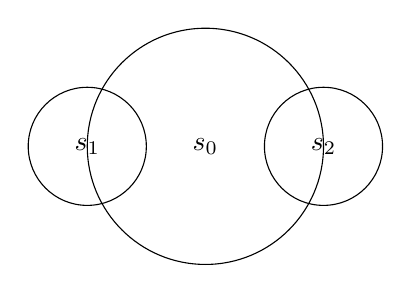
\begin{tikzpicture}[scale=0.75]
  \draw
    (0,0)
    circle
    [radius=2]
    node {$s_{0}$};
  \draw
    (-2,0)
    circle
    [radius=1]
    node {$s_{1}$};
  \draw
    (2,0)
    circle
    [radius=1]
    node {$s_{2}$};
\end{tikzpicture}
\]
Then $(\mathrm{res}_{1}(s_{0},s_{1},s_{2}))(s_{0})$ is illustrated by the three diagrams
\[
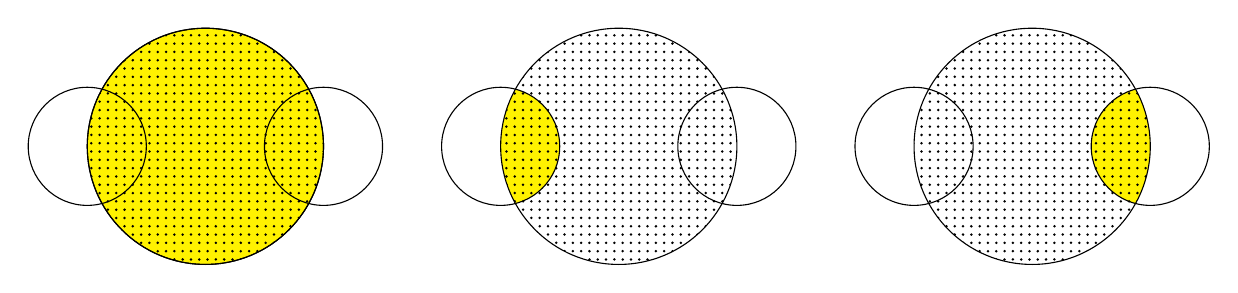
\begin{tikzpicture}[scale=0.75]
\begin{scope}
  \clip
    (0,0)
    circle
    [radius=2];
  \fill[fill=yellow]
    (-2,0)
    circle
    [radius=1];
  \clip
    (2,0)
    circle
    [radius=1];
\end{scope}
\begin{scope}
  \clip
    (7,0)
    circle
    [radius=2];
  \fill[fill=yellow]
    (9,0)
    circle
    [radius=1];
  \clip
    (5,0)
    circle
    [radius=1];
\end{scope}
  \filldraw[fill=yellow]
    (-7,0)
    circle
    [radius=2];
  \draw[pattern=dots]
    (-7,0)
    circle
    [radius=2];
  \draw
    (-9,0)
    circle
    [radius=1];
  \draw
    (-5,0)
    circle
    [radius=1];
  \draw[pattern=dots]
    (0,0)
    circle
    [radius=2];
  \draw
    (-2,0)
    circle
    [radius=1];
  \draw
    (2,0)
    circle
    [radius=1];
  \draw[pattern=dots]
    (7,0)
    circle
    [radius=2];
  \draw
    (5,0)
    circle
    [radius=1];
  \draw
    (9,0)
    circle
    [radius=1];
\end{tikzpicture}
\]
while $(\mathrm{res}_{2}(s_{0},s_{1},s_{2}))(s_{0})$ is illustrated by the three diagrams
\[
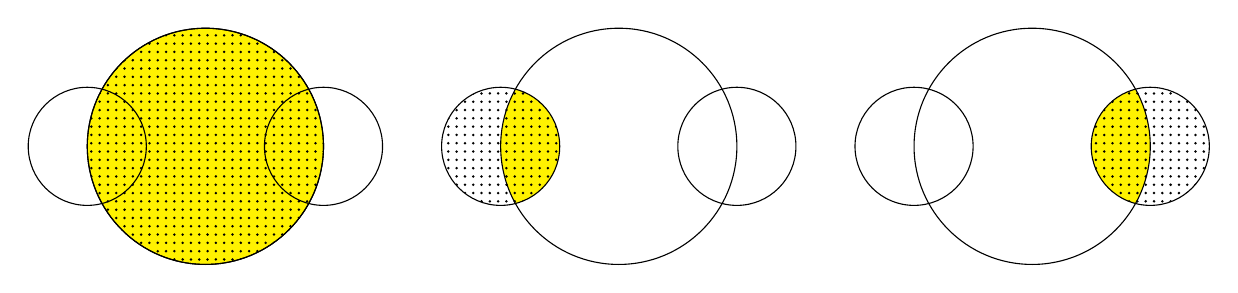
\begin{tikzpicture}[scale=0.75]
\begin{scope}
  \clip
    (0,0)
    circle
    [radius=2];
  \fill[fill=yellow]
    (-2,0)
    circle
    [radius=1];
  \clip
    (2,0)
    circle
    [radius=1];
\end{scope}
\begin{scope}
  \clip
    (7,0)
    circle
    [radius=2];
  \fill[fill=yellow]
    (9,0)
    circle
    [radius=1];
  \clip
    (5,0)
    circle
    [radius=1];
\end{scope}
  \filldraw[fill=yellow]
    (-7,0)
    circle
    [radius=2];
  \draw[pattern=dots]
    (-7,0)
    circle
    [radius=2];
  \draw
    (-9,0)
    circle
    [radius=1];
  \draw
    (-5,0)
    circle
    [radius=1];
  \draw
    (0,0)
    circle
    [radius=2];
  \draw[pattern=dots]
    (-2,0)
    circle
    [radius=1];
  \draw
    (2,0)
    circle
    [radius=1];
  \draw
    (7,0)
    circle
    [radius=2];
  \draw
    (5,0)
    circle
    [radius=1];
  \draw[pattern=dots]
    (9,0)
    circle
    [radius=1];
\end{tikzpicture}
\]
if the dotted areas correspond to the first index $k_{1}$ we fix and the second index $k_{2}$ corresponds to the three diagrams. The restriction results are always the color filled areas. We hope this illustration helps a bit. Anyways, in the end we get for a space $S$ a full subcategory
\begin{align*}
  \mathbf{Sh}(S)
\end{align*}
of
\begin{align*}
  \mathbf{Set}^{\mathbf{Open}_{S}^{\mathrm{op}}}
\end{align*}
by restricting the object set to sheaves on $\mathbf{Open}_{S}$. $\mathbf{Sh}(S)$ is called the \textbf{category of sheaves (on $S$)}
\\
Note that this definition also makes sense in other categories than $\mathbf{Set}$. The category must only have enough limits. In particular the sheaf definition makes sense for $\mathbf{C}_{\alpha}$-valued presheaves if $\mathbf{C}_{\alpha}$ is complete. In fact, $\mathbf{Grp}$-valued sheaves are common (and a few others). But one can also think of $\mathbf{Grp}$-valued sheaves as internalization (see subsection \ref{sec:internaliz}). Namely as group object (again see subsection \ref{sec:internaliz}) in $\mathbf{Sh}(S)$ since this category as topos (see subsection \ref{sec:internaliz}) has enough structure to allow these.
\\
We almost achieved our goal of formulating the second consistency condition by the descent condition. What is missing is a more general notion sensibly replacing $\mathbf{Open}_{S}$ by any category with a reasonable notion of (open) cover. Note that $\mathrm{Mor}_{\mathbf{Open}_{S}}$ has the property that
\begin{align*}
  \mathrm{i}_{U_{2}}
  \in
  \mathrm{Mor}_{\mathbf{Open}_{S}}
\end{align*}
implies that for all
\begin{align*}
  \mathrm{i}_{12}
  \in
  \mathrm{Mor}_{\mathbf{Open}_{S}}
\end{align*}
with
\begin{align*}
  \mathrm{dom}_{\mathbf{Open}_{S}}(\mathrm{i}_{U_{2}})
  &=
  \mathrm{cod}_{\mathbf{Open}_{S}}(\mathrm{i}_{12})
\end{align*}
we have
\begin{align*}
  \mathrm{i}_{U_{2}}
  \circ
  \mathrm{i}_{12}
  \in
  \mathrm{Mor}_{\mathbf{Open}_{S}}
\end{align*}
This can be interpreted as $\mathrm{i}_{U_{2}}$ punching a hole into $S$ in the form of $U_{2}$ and any $U_{1}$ smaller than $U_{2}$ fits through this hole. As a picture
\[
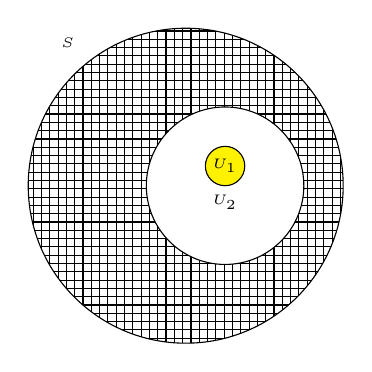
\begin{tikzpicture}[scale=0.25]
  \draw[pattern=grid]
    (0,0)
    circle
    [radius=8];
  \filldraw[fill=white]
    (2,0)
    circle
    [radius=4];
  \filldraw[fill=yellow]
    (2,1)
    circle
    [radius=1]
    node {\tiny{$U_{1}$}};
  \draw
    (-6,8)
    --
    (-6,8)
    node [below] {\tiny{$S$}};
  \draw
    (2,0)
    --
    (2,0)
    node [below] {\tiny{$U_{2}$}};
\end{tikzpicture}
\]
It is clear that this has to do with covers. And the idea works in general for any category since given a category $\mathbf{C}$ and an object $X$ then a subset $\mathfrak{S}_{X} \subset \mathrm{Mor}_{\mathbf{C}}$ such that
\begin{align*}
  f
  \in
  \mathfrak{S}_{X}
  \quad
  &\Rightarrow
  \quad
  \mathrm{cod}_{\mathbf{C}}(f)
  =
  X
\end{align*}
is called a \textbf{sieve (on $X$)} if
\begin{enumerate}
\item[({\#})]
for all $f \in \mathfrak{S}_{X}$ and for all $i \in \mathrm{Mor}_{\mathbf{C}}$ such that
\begin{align*}
  \mathrm{dom}_{\mathbf{C}}(f)
  &=
  \mathrm{cod}_{\mathbf{C}}(i)
\end{align*}
we have
\begin{align*}
  f
  \circ
  i
  \in
  \mathfrak{S}_{X}
\end{align*}
\end{enumerate}
It is clear that
\begin{align*}
  \mathfrak{M}_{X}
  &:=
  \bigcup_{X \in \mathrm{ob}_{\mathbf{C}}}
  \mathrm{mor}_{\mathbf{C}}(X,X_{0})
\end{align*}
is a sieve on $X_{0}$ and we call it the \textbf{maximal sieve (on $X_{0}$)}. We would still like to think of a sieve on $X$ as a cover of $X$ but we gave up on the injectivity of morphisms by this generalization which was crucial in the topological case. Hence we have to make up for this loss by demanding some properties which make the idea sufficiently close to covers. So let's see what properties we can abstract from $\mathbf{Open}_{S}$.
\begin{enumerate}
\item[(1)]
For any open subspace $U$ of $S$ we can cover $U$ by the collection of all the open subspaces of $U$. In terms of sieves we can express that by demanding the maximal sieve on $U$ to cover $U$.
\item[(2)]
Given an open subspace $U$ of $S$ which is covered by some $U_{k}$ indexed by some small set $K$ then we can clearly intersect $U$ with some other open subspace $U^{\backprime}$ of $S$ and it is clear that $U_{k} \cap U^{\backprime}$ for $k \in K$ covers $U \cap U^{\backprime}$.
\item[(3)]
Given an open subspace $U$ of $S$ which is covered by some $U_{k}$ indexed by some small set $K$ and for each $U_{k}$ a cover consisting of sets $(U_{k})_{l_{k}}$ indexed by $l_{k} \in L_{k}$ with $L_{k}$ a small set for all $k \in K$ then clearly all the $(U_{k})_{l_{k}}$ can be taken together to cover $U$.
\end{enumerate}
These ideas will yield the definition of Grothendieck topology. But we still need one last ingredient. We must somehow express the intersection in categorical terms. And here the pullback from example \ref{exa:oflimits} puts itself forward. Given a sieve $\mathfrak{S}_{X}$ and a $f \in \mathrm{Mor}_{\mathbf{C}}$ then 
\begin{align*}
  f^{\ast}(\mathfrak{S}_{X})
  &:=
  \lbrace
      h
      \in
      \mathrm{Mor}_{\mathbf{C}}
    \,
    \vert
    \,
      f
      \circ
      h
      \in
      \mathfrak{S}_{X}
  \rbrace
\end{align*}
is a sieve on $\mathrm{dom}_{\mathbf{C}}(f)$ since for $h \in f^{\ast}(\mathfrak{S}_{X})$ and all $h^{\backprime} \in \mathrm{Mor}_{\mathbf{C}}$ such that
\begin{align*}
  \mathrm{dom}_{\mathbf{C}}(h)
  &=
  \mathrm{cod}_{\mathbf{C}}(h^{\backprime})
\end{align*}
we have
\begin{align*}
  \mathrm{dom}_{\mathbf{C}}(f \circ h)
  &=
  \mathrm{cod}_{\mathbf{C}}(h^{\backprime})
\end{align*}
Thus, because $\mathfrak{S}_{X}$ containing $f \circ h$ is a sieve we can conclude
\begin{align*}
  f
  \circ
  h
  \circ
  h^{\backprime}
  &\in
  \mathfrak{S}_{X}
\end{align*}
which is to say that
\begin{align*}
  h
  \circ
  h^{\backprime}
  &\in
  f^{\ast}(\mathfrak{S}_{X})
\end{align*}
proving the claim. We then call $f^{\ast}(\mathfrak{S}_{X})$ the \textbf{pullback sieve (of $\mathfrak{S}_{X}$ along $f$)}. Indeed, it can be shown that this is actually a pullback in $\mathbf{Set}^{\mathbf{C}^{\mathrm{op}}}$. This is since sieves correspond to presheaves which can be reasonably included into representable presheaves. This inclusion is then pulled back along $\mathrm{y}_{\mathbf{C}}(f)$. Details can be found in the source we will cite in a moment. But now to Grothendieck topologies. Given a small category $\mathbf{C}$ a \textbf{Grothendieck topology (on $\mathbf{C}$)} is a function
\begin{align*}
  \mathrm{J}
  \colon
  \mathrm{ob}_{\mathbf{C}}
  &\rightarrow
  \mathrm{ob}_{\mathbf{Set}}
\end{align*}
such that each $\mathfrak{S}_{X} \in \mathrm{J}(X)$ is a sieve on $X$ for all $X$ satisfying
\begin{enumerate}
\item[(J1)]
the maximal sieve $\mathfrak{M}_{X}$ is in $\mathrm{J}(X)$ for all $X$
\item[(J2)]
if $\mathfrak{S}_{X} \in \mathrm{J}(X)$ then for any $f$ with codomain $X$ the pullback sieve $f^{\ast}(\mathfrak{S}_{X})$ is element of $\mathrm{J}(\mathrm{dom}_{\mathbf{C}}(f))$
\item[(J3)]
if $\mathfrak{S}_{X} \in \mathrm{J}(X)$ and $\mathfrak{S}_{X}^{\backprime}$ is a sieve on $X$ such that for all $f \in \mathfrak{S}_{X}$
\begin{align*}
  f^{\ast}
  \left(
    \mathfrak{S}_{X}^{\backprime}
  \right)
  &\in
  \mathrm{J}
  \left(
    \mathrm{dom}_{\mathbf{C}}(f))
  \right)
\end{align*}
then $\mathfrak{S}_{X}^{\backprime}$ is element of $\mathrm{J}(X)$.
\end{enumerate}
For a Grothendieck topology $\mathrm{J}$ we call $\mathfrak{S}_{X} \in \mathrm{J}(X)$ a \textbf{covering sieve (on $X$ w.r.t. $\mathrm{J}$)} while the pair $(\mathbf{C},\mathrm{J})$ is called a \textbf{site}.
\\
Sites are sufficient to define what it means for a presheaf on a site to be a sheaf. So assume a site $(\mathbf{C},\mathrm{J})$. Then a presheaf $P$ on $\mathbf{C}$ is a \textbf{sheaf (on $(\mathbf{C},\mathrm{J})$)} if
\begin{enumerate}
\item[(DC)]
for each object $X$ and each covering sieve $\mathfrak{S}_{X} \in \mathrm{J}(X)$ the pair $(P(X),e)$ with
\begin{align*}
  e
  \colon
  P(X)
  &\rightarrow
  \prod_{f \in \mathfrak{S}_{X}}
  P(\mathrm{dom}_{\mathbf{C}}(f))
  \\
  s
  &\mapsto
  (P(f))(s)
\end{align*}
is the equalizer of
\begin{align*}
  \mathrm{res}_{1}
  \colon
  \prod_{f \in \mathfrak{S}_{X}}
  P(\mathrm{dom}_{\mathbf{C}}(f))
  &\rightarrow
  \prod_{f \in \mathfrak{S}_{X}}
  \prod_{h \in f^{\ast}(\mathfrak{S}_{X})}
  P(\mathrm{dom}_{\mathbf{C}}(h))  
  \\
  \left(
    f
    \mapsto
    s_{f}
  \right)
  &\mapsto
  \left(
    f
    \mapsto
    \left(
      h
      \mapsto
      s_{f \circ h}
    \right)
  \right)
  \\\\
  \mathrm{res}_{2}
  \colon
  \prod_{f \in \mathfrak{S}_{X}}
  P(\mathrm{dom}_{\mathbf{C}}(f))
  &\rightarrow
  \prod_{f \in \mathfrak{S}_{X}}
  \prod_{h \in f^{\ast}(\mathfrak{S}_{X})}
  P(\mathrm{dom}_{\mathbf{C}}(h))  
  \\
  \left(
    f
    \mapsto
    s_{f}
  \right)
  &\mapsto
  \left(
    f
    \mapsto
    \left(
      h
      \mapsto
      P(h)(s_{f})
    \right)
  \right)
\end{align*}
\end{enumerate}
We refer to (DC) as \textbf{descent condition (for sheaves on $(\mathbf{C},\mathrm{J})$)} or sometimes equivalently \textbf{sheaf condition (on $(\mathbf{C},\mathrm{J})$)}. There is a site on $\mathbf{Open}_{S}$ such that the sheaf condition on that site is the sheaf condition on $\mathbf{Open}_{S}$. We have now a whole lot of possible categories of spaces. In particular there are sites on categories with objects some manifolds. This fact should make physicists prick up their ears.
\\
We have to admit here that what we have written is a bit sketchy on the motivational side. But you can convince yourself that all this is sensible by reading the first three to four chapters of the somehow worthwhile book \cite{c55c71e8}. You will then see that what we have described here is only the tip of the iceberg of some beautiful mathematics. We will mention the book again when we come to topoi in subsection \ref{sec:internaliz}.
\end{exa}
\begin{prf}
You might wish to prove here that $\Gamma_{\pi}$ is in fact a sheaf on $\mathbf{Open}_{S}$. This is essentially the topological fact that continuity is a local property and the theorem that a bunch of locally given continuous functions patch together - or better say extend here - to a unique continuous function which can be found in any topology book such as \cite{273ba834}.
\\
\phantom{proven}
\hfill
$\square$
\end{prf}
We have one last thing on limits that will be very convenient. Motivated from analysis we would like to define a sensible functor mapping functors $F$ to the apex of their (co)limiting (co)cone like one does in analysis when mapping a sequence to its limit. To this end let $F \colon \mathbf{J} \rightarrow \mathbf{C}$ be a functor with $\mathbf{J}$ small and $\mathbf{C}$ locally small. Then define the sets
\begin{align*}
  \mathrm{Lim}_{F}
  &:=
  \left\lbrace
      (X_{T},F,\mathsf{C}_{T})
      \in
      \mathrm{ob}_{(\Delta_{\mathbf{C}} \downarrow \mathrm{c}_{F})}
    \vert
      (X_{T},F,\mathsf{C}_{T})
      \text{ is a limit of }
      F
  \right\rbrace
\end{align*}
if $\mathbf{C}$ is complete and
\begin{align*}
  \mathrm{Colim}_{F}
  &:=
  \left\lbrace
      (F,X_{I},\mathsf{C}_{I}^{\prime})
      \in
      \mathrm{ob}_{(\mathrm{c}_{F} \downarrow \Delta_{\mathbf{C}})}
    \vert
      (F,X_{I},\mathsf{C}_{I}^{\prime})
      \text{ is a colimit of }
      F
  \right\rbrace
\end{align*}
if $\mathbf{C}$ is cocomplete. To achieve our goal we first need to define functions mapping functors $F$ to an element of $\mathrm{Lim}_{F}$ and $\mathrm{Colim}_{F}$, respectively. So we have to choose an element of $\mathrm{Lim}_{F}$ and $\mathrm{Colim}_{F}$, respectively, for all $F$. But the axiom of choice of TG asserts that dependent functions
\begin{align*}
  c_{\mathrm{Lim}}
  &\in
  \prod_{F \in \mathrm{ob}_{\mathbf{C}^{\mathbf{J}}}}
  \mathrm{Lim}_{F}
  \\
  c_{\mathrm{Colim}}
  &\in
  \prod_{F \in \mathrm{ob}_{\mathbf{C}^{\mathbf{J}}}}
  \mathrm{Colim}_{F}
\end{align*}
exist. To this we have an important remark.
\\
\begin{rem}
\label{rem:ordinaltrick}
Note that it is not clear that $\mathrm{Lim}_{F}$ and $\mathrm{Colim}_{F}$ are small sets and foundations such as ZFC and von Neumann-Bernays-G\"odel (abbr. NGB) lack a choice axiom powerful enough to choose from such large collections. But there is a trick with well-orders which shows how to make this still possible. The axiom of choice does only grant existence but it does not explicitly tell us what is chosen. This is actually not very nice. If, however, we constrained first-order logic to intuitionistic logic then we would have to contruct a limit/colimit explicitly to show that it exists and the axiom of choice would be superfluous here since we could define a choice function as above by just proving that the limits/colimits exist for all $F$. Hence an intuitionist does not need the axiom of choice to do the same as we do here. Indeed, in category theory it is common to work with intuitionistic logic if possible and we use the axiom of choice here only for the sake of rigor. Many authors ignore the issue due to this common practice since they think limits/colimits are constructed anyway in practice. Also note that in UFP-HoTT the issue is not really an issue since it is usually assumed intuitionistic (and all limits/colimits are formally equal by univalence). The same issue in another guise will arise for adjoints in subsection \ref{sec:adjoint} an we will refer back to this remark.
\end{rem}
\begin{prf}
The ordnial trick we addressed can be found in \cite{53fd7d7e} in chapter 7 footnote 7.
\\
\phantom{proven}
\hfill
$\square$
\end{prf}
On the whole any choice function as above yields a function mapping functors to a limit of it and the same for colimits. This function can be made into a functor as can be seen from the following discussion. So take $G_{1},G_{2} \in \mathrm{ob}_{\mathbf{C}^{\mathbf{J}}}$ and a natural transformation $\mathsf{T} \colon G_{1} \Rightarrow G_{2}$.
\begin{align*}
  \left(
    X_{T}^{k},
    G_{k},
    \mathsf{C}_{T}^{k}
  \right)
\end{align*}
shall denote a limiting cone to $G_{k}$ with apex $X_{T}^{k}$ for $k = 1,2$. Then there is a unique morphism
\begin{align*}
  \mathsf{T}_{!}
  &\in
  \mathrm{mor}_{\mathbf{C}}
  \left(
    X_{T}^{1},
    X_{T}^{2}
  \right)
\end{align*}
determined by the commutative diagram
\[
\begin{tikzcd}[row sep=huge, column sep=9em]
  G_{1}(J_{1})
  \arrow{rr}{G_{1}(j_{12})}
  \arrow[swap]{ddd}{\mathsf{T}(J_{1})}
  &
  &
  G_{1}(J_{2})
  \arrow{ddd}{\mathsf{T}(J_{2})}
  \\
  &
  X_{T}^{1}
  \arrow{ur}{\mathsf{C}_{T}^{1}(J_{2})}
  \arrow[dashed]{d}{\mathsf{T}_{!}}
  \arrow[swap]{ul}{\mathsf{C}_{T}^{1}(J_{1})}
  &
  \\
  &
  X_{T}^{2}
  \arrow[swap]{dr}{\mathsf{C}_{T}^{2}(J_{2})}
  \arrow{dl}{\mathsf{C}_{T}^{2}(J_{1})}
  &
  \\
  G_{2}(J_{1})
  \arrow{rr}{G_{2}(j_{12})}
  &
  &
  G_{2}(J_{2})
\end{tikzcd}
\]
This works since $\mathsf{T} \circ \mathsf{C}_{T}^{1}$ is a cone to $G_{2}$ with apex $X_{T}^{1}$. Dually, let
\begin{align*}
  \left(
    G_{k},
    X_{I}^{k},
    \mathsf{C}_{I}^{k}
  \right)
\end{align*}
denote a colimiting cocone to $G_{k}$ with apex $X_{I}^{k}$ for $k = 1,2$. Then there is a unique morphism
\begin{align*}
  \mathsf{T}_{!}^{\prime}
  &\in
  \mathrm{mor}_{\mathbf{C}}
  \left(
    X_{I}^{1},
    X_{I}^{2}
  \right)
\end{align*}
determined by the commutative diagram
\[
\begin{tikzcd}[row sep=huge, column sep=9em]
  G_{1}(J_{1})
  \arrow{rr}{G_{1}(j_{12})}
  \arrow[swap]{ddd}{\mathsf{T}(J_{1})}
  \arrow{dr}{\mathsf{C}_{I}^{1}(J_{1})}
  &
  &
  G_{1}(J_{2})
  \arrow[swap]{dl}{\mathsf{C}_{I}^{1}(J_{2})}
  \arrow{ddd}{\mathsf{T}(J_{2})}
  \\
  &
  X_{I}^{1}
  \arrow[dashed]{d}{\mathsf{T}_{!}^{\prime}}
  &
  \\
  &
  X_{I}^{2}
  &
  \\
  G_{2}(J_{1})
  \arrow[swap]{ur}{\mathsf{C}_{I}^{2}(J_{1})}
  \arrow{rr}{G_{2}(j_{12})}
  &
  &
  G_{2}(J_{2})
  \arrow{ul}{\mathsf{C}_{I}^{2}(J_{2})}
\end{tikzcd}
\]
This works again since $\mathsf{C}_{I}^{2} \circ \mathsf{T}$ is a cocone to $G_{1}$ with apex $X_{I}^{2}$. Now we are sufficiently prepared to define the functors. Given the choice functions $c_{\mathrm{Lim}}$ and $c_{\mathrm{Colim}}$ we can define functors
\begin{align*}
  \varprojlim_{\mathbf{J}}
  \doteq
  \varprojlim_{\mathbf{J}}^{c_{\mathrm{Lim}}}
  \colon
  \mathbf{C}^{\mathbf{J}}
  &\rightarrow
  \mathbf{C}
  \\
  F
  &\mapsto
  \mathrm{pr}_{1}
  \circ
  c_{\mathrm{Lim}}(F)
  \\
  \mathsf{T}
  &\mapsto
  \mathsf{T}_{!}
  \\
  \\
  \varinjlim_{\mathbf{J}}
  \doteq
  \varinjlim_{\mathbf{J}}^{c_{\mathrm{Colim}}}
  \colon
  \mathbf{C}^{\mathbf{J}}
  &\rightarrow
  \mathbf{C}
  \\
  F
  &\mapsto
  \mathrm{pr}_{2}
  \circ
  c_{\mathrm{colim}}(F)
  \\
  \mathsf{T}
  &\mapsto
  \mathsf{T}_{!}^{\prime}
\end{align*}
$\varprojlim_{\mathbf{J}}^{c_{\mathrm{Lim}}}$ is called \textbf{limit functor (for $c_{\mathrm{Lim}}$ over $\mathbf{J}$)} while $\varinjlim_{\mathbf{J}}^{c_{\mathrm{Colim}}}$ is called \textbf{colimit functor (for $c_{\mathrm{colim}}$ over $\mathbf{J}$)}. The convention is that the choice functions $c_{\mathrm{Lim}}$ and $c_{\mathrm{Colim}}$ are silently assumed to be the canonical ones obtained from constructing the limits explicitly if possible (which is practically always possible in category theory) and else the choice functions obtained from the axiom of choice when technically necessary. Again, it is common not to mention them in practice and so will we do in the following. As a last remark here, limit and colimit functors for different choice functions are naturally isomorphic as is apparent essentially from theorem \ref{thm:uniqueuniarr} which implies that limits are unique up to unique isomorphism. So structurally the choice function is not essential.
\\\\
We are now able to prove the last fact about bicompleteness we need. It is that functor categories are bicomplete if the codomain category is.
\\
\begin{thm}
\label{thm:funccatbicomplete}
Let $\mathbf{C}$ be small.
\begin{enumerate}
\item[(1T)]
If $\mathbf{C}_{\alpha}$ is complete then so is $\mathbf{C}_{\alpha}^{\mathbf{C}}$.
\item[(1I)]
If $\mathbf{C}_{\alpha}$ is cocomplete then so is $\mathbf{C}_{\alpha}^{\mathbf{C}}$.
\end{enumerate}
\end{thm}
\begin{prf}
\begin{enumerate}
\item[(1T)]
Let
\begin{align*}
  F
  \colon
  \mathbf{J}
  &\rightarrow
  \mathbf{C}_{\alpha}^{\mathbf{C}}
\end{align*}
be a functor. By premise, we have a limiting cone $\mathsf{C}_{T}^{X}$ to $(F(\cdot))(X)$ with apex
\begin{align*}
  \varprojlim_{\mathbf{J}}
  \left(
    (F(\cdot))(X)
  \right)
\end{align*}
and we can define a functor
\begin{align*}
  \varprojlim^{F}
  \colon
  \mathbf{C}
  &\rightarrow
  \mathbf{C}_{\alpha}
  \\
  X
  &\mapsto
  \varprojlim_{\mathbf{J}}
  \left(
    (F(\cdot))(X)
  \right)
  \\
  f_{12}
  &\mapsto
  \varprojlim_{\mathbf{J}}
  \left(
    (F(\cdot))(f_{12})
  \right)
\end{align*}
Hence we can define a cone $\mathsf{C}_{T}$ to $F$ by mapping $J$ to the natural transformation
\begin{align*}
  \mathsf{C}_{T}(J)
  \colon
  \varprojlim^{F}
  &\Rightarrow
  F(J)
  \\
  X
  &\mapsto
  \mathsf{C}_{T}^{X}(J)
\end{align*}
Once more we proceed in two steps to finish the proof.
\begin{description}
\item[Step 1]
$\mathsf{C}_{T}$ is in fact a cone since
\begin{align*}
  \left(
    F(j_{12})
    \circ
    \mathsf{C}_{T}(J_{1})
  \right)
  (X)
  &=
  (F(j_{12}))(X)
  \circ
  \left(
    \mathsf{C}_{T}(J_{1})
  \right)
  (X)
  \\
  &=
  (F(j_{12}))(X)
  \circ
  \mathsf{C}_{T}^{X}(J_{1})
  \\
  &=
  \mathsf{C}_{T}^{X}(J_{2})
  \\
  &=
  \left(
    \mathsf{C}_{T}(J_{2})
  \right)
  (X)
\end{align*}
for all $j_{12}$ and $X$.
\item[Step 2]
$\mathsf{C}_{T}$ is also limiting since for any cone $\mathsf{C}$ to $F$ with apex $G \colon \mathbf{C} \rightarrow \mathbf{C}_{\alpha}$ we have that $(\mathsf{C}(\cdot))(X)$ is a cone to $(F(\cdot))(X)$ for all $X$ and by premise there is a unique
\begin{align*}
  \mathsf{C}_{!}^{X}
  \in
  \mathrm{mor}_{\mathbf{C}_{\alpha}}
  \left(
    G(X),
    \varprojlim^{F}(X)
  \right)
\end{align*}
such that
\begin{align*}
  \mathsf{C}_{T}^{X}(J)
  \circ
  \mathsf{C}_{!}^{X}
  &=
  (\mathsf{C}(J))(X)
\end{align*}
for all $J$. Hence the natural transformation
\begin{align*}
  \mathsf{C}_{!}
  \colon
  G
  &\Rightarrow
  \varprojlim^{F}
  \\
  X
  &\mapsto
  \mathsf{C}_{!}^{X}
\end{align*}
is the unique morphism such that
\begin{align*}
  \left(
    \mathsf{C}_{T}(J)
    \circ
    \mathsf{C}_{!}
  \right)
  (X)
  &=
  \left(
    \mathsf{C}_{T}(J)
  \right)
  (X)
  \circ
  \mathsf{C}_{!}(X)
  \\
  &=
  \mathsf{C}_{T}^{X}(J)
  \circ
  \mathsf{C}_{!}^{X}
  \\
  &=
  (\mathsf{C}(J))(X)
\end{align*}
\end{description}
\item[(1I)]
The duality principle \ref{thm:dp}.
\end{enumerate}
\phantom{proven}
\hfill
$\square$
\end{prf}
Hence in the case of completeness limits are computed {\glqq}pointwise{\grqq} and so are colimits in case of cocompleteness. But if we are not complete or cocomplete this is not necessarily the case. 

\subsubsection{Co-Yoneda I}
\label{sec:coyoneda1}
This subsubsection is about a consequence of the so-called Co-Yoneda lemma that owes its name to being some kind of dual to the actual yoneda lemma \ref{lem:yoneda}. The Co-Yoneda lemma is discussed and formulated in subsubsection \ref{sec:coyoneda2} after we have developed some more machinery. The consequence we discuss in this subsubsection with more elementary means is the so-called density theorem.  What it actually says is that any presheaf $P$ on $\mathbf{C}$ is the colimit of contravariant hom-functors indexed by the category of colements of $P$. That is, the representable presheaves on $\mathbf{C}$ as generalized objects are enough to build any generalized object in the presheaf category by gluing the representable generalized objects together. Gluing objects together is the very idea of a colimit as should have become clear from this subsection \ref{sec:limit}. This will become even clearer when the objects have a geometric meaning as in section \ref{sec:sset} where they are considered as triangles. One can also interpret colimit a bit as a kind of limiting process similar to limits in analysis. By that we mean that presheaves are {\glqq}approximated{\grqq} well enough by representable presheaves which is why people consider density theorem a suitable name for the following theorem.
\\
\begin{thm}[Density]
\label{thm:density}
Let $P \colon \mathbf{C}^{\mathrm{op}} \rightarrow \mathbf{Set}_{\mathcal{U}}$ be a presheaf on a $\mathcal{U}$-small $\mathbf{C}$ and define a projection functor on the category of coelements of $P$ by
\begin{align*}
  \pi_{P}
  \colon
  \int_{\mathbf{C}}^{\prime}
  P
  &\rightarrow
  \mathbf{C}
  \\
  (X,x)
  &\mapsto
  X
  \\
  f_{21}^{\mathrm{op}}
  &\mapsto
  f_{12}
\end{align*}
Further compose this functor with the Yoneda functor as
\begin{align*}
  \mathrm{y}_{P}
  &:=
  \mathrm{y}_{\mathbf{C}}
  \circ
  \pi_{P}
\end{align*}
and define a function
\begin{align*}
  \mathsf{C}_{P}^{\prime}
  \colon
  \mathrm{ob}_{\int_{\mathbf{C}}^{\prime}P}
  &\rightarrow
  \bigcup_{X \in \mathrm{ob}_{\mathbf{C}^{\mathrm{op}}}}
  \mathrm{mor}_{\mathbf{Set}^{\mathbf{C}^{\mathrm{op}}}}
  \left(
    \mathrm{y}_{\mathbf{C}}(X),
    P
  \right)
  \\
  (X,x)
  &\mapsto
  \mathsf{Y}(P,X)^{-1}(x)
\end{align*}
where $\mathsf{Y}(P,X)$ denotes the Yoneda isomorphism. Then $\mathsf{C}_{P}^{\prime}$ is a colimiting cocone for $\mathrm{y}_{P}$ with apex $P$. Hence
\begin{align*}
  P
  &\cong
  \varinjlim_{\int_{\mathbf{C}}^{\prime}P}(\mathrm{y}_{P})
\end{align*}
\end{thm}
\begin{prf}
As always in such situations we proceed in two steps. We first show that $\mathsf{C}_{P}^{\prime}$ is a cocone and then that it is colimiting.
\begin{description}
\item[Step 1]
We will incorporate the Yoneda lemma \ref{lem:yoneda} to show that $\mathsf{C}_{P}^{\prime}$ is a cocone. Consider
\begin{align*}
  (X_{1},x_{1}),
  (X_{2},x_{2})
  \in
  \mathrm{ob}_{\int_{\mathbf{C}}^{\prime}P}
\end{align*}
Then
\begin{align*}
  x_{1}
  &=
  P(f_{21}^{\mathrm{op}})(x_{2})
\end{align*}
holds for all
\begin{align*}
  f_{21}^{\mathrm{op}}
  \in
  \mathrm{mor}_{\int_{\mathbf{C}}^{\prime}P}
  \left(
    (X_{1},x_{1}),
    (X_{2},x_{2})
  \right)
\end{align*}
Applying the Yoneda isomorphism and using its naturality then yields the equivalent equation
\begin{align*}
  \mathsf{Y}(P,X_{1})^{-1}(x_{1})
  &=
  \left(
    \mathsf{Y}(P,X_{1})^{-1}
    \circ
    P(f_{21}^{\mathrm{op}})
    \circ
    \mathsf{Y}(P,X_{2})
    \circ
    \mathsf{Y}(P,X_{2})^{-1}
  \right)
  (x_{2})
  \\
  &=
  \mathrm{prob}_{\mathrm{y}}(\mathrm{id}_{P},f_{21}^{\mathrm{op}})
  \left(
    \mathsf{Y}(P,X_{2})^{-1}(x_{2})
  \right)
  \tag{NT}
  \\
  &=
  \mathsf{Y}(P,X_{2})^{-1}(x_{2})
  \circ
  \mathrm{y}_{\mathbf{C}}(f_{21}^{\mathrm{op}})
\end{align*}
Hence by definition of $\mathsf{C}_{P}^{\prime}$ this implies a commutative diagram
\[
\begin{tikzcd}[sep=huge]
  \mathrm{y}_{\mathbf{C}}(X_{1})
  \arrow{rr}{\mathrm{y}_{\mathbf{C}}(f_{21}^{\mathrm{op}})}
  \arrow[swap]{dr}{\mathsf{C}_{P}^{\prime}(X_{1},x_{1})}
  &
  &
  \mathrm{y}_{\mathbf{C}}(X_{2})
  \arrow{dl}{\mathsf{C}_{P}^{\prime}(X_{2},x_{2})}
  \\
  &
  P
  &
\end{tikzcd}
\]
finally showing that $\mathsf{C}_{P}^{\prime}$ is a cocone. 
\\
\item[Step 2]
Let $\mathsf{C}^{\prime}$ denote any cocone to $\mathrm{y}_{P}$ with apex $P^{\backprime}$. We can then apply the Yoneda isomorphism $\mathsf{Y}(P^{\backprime},X)$ to $\mathsf{C}^{\prime}(X,x)$ to get the corresponding element in $P^{\backprime}(X)$ for each
\begin{align*}
  (X,x)
  \in
  \mathrm{ob}_{\int_{\mathbf{C}}^{\prime}P}
\end{align*}
Let us denote this by
\begin{align*}
  \mathrm{y}_{(X,x)}^{\backprime}
  &:=
  \mathsf{Y}(P^{\backprime},X)
  \left(
    \mathsf{C}^{\prime}(X,x)
  \right)
\end{align*}
We have to find a unique natural transformation $\mathsf{T}$ from $P$ to $P^{\backprime}$ such that
\begin{align*}
  \mathsf{C}^{\prime}(X,x)
  &=
  \mathsf{T}
  \circ
  \mathsf{C}_{P}^{\prime}(X,x)
\end{align*}
for all
\begin{align*}
  (X,x)
  \in
  \mathrm{ob}_{\int_{\mathbf{C}}^{\prime}P}
\end{align*}
We propose defining $\mathsf{T}$ by mapping an object $X$ to
\begin{align*}
  \mathsf{T}(X)
  \colon
  P(X)
  &\rightarrow
  P^{\backprime}(X)
  \\
  x
  &\mapsto
  \mathrm{y}_{(X,x)}^{\backprime}
\end{align*}
Since $\mathsf{Y}$ is natural, for arbitrary $f_{21}^{\mathrm{op}}$ and $x_{1} \in P(X_{1})$
the equations
\begin{align*}
  \left(
    P^{\backprime}(f_{21}^{\mathrm{op}})
    \circ
    \mathsf{T}(X_{2})
  \right)
  (x_{2})
  &=
  P^{\backprime}(f_{21}^{\mathrm{op}})
  \left(
    \mathrm{y}_{(X_{2},x_{2})}^{\backprime}
  \right)
  \\
  &=
  P^{\backprime}(f_{21}^{\mathrm{op}})
  \left(
    \mathsf{Y}(P^{\backprime},X_{2})
    \left(
      \mathsf{C}^{\prime}(X_{2},x_{2})
    \right)
  \right)
  \\
  &=
  \mathsf{Y}(P^{\backprime},X_{1})
  \left(
    \mathrm{prob}_{\mathrm{y}}
    \left(
      \mathrm{id}_{P^{\backprime}},
      f_{21}^{\mathrm{op}}
    \right)
    \left(
      \mathsf{C}^{\prime}(X_{2},x_{2})
    \right)
  \right)
  \tag{NT}
  \\
  &=
  \mathsf{Y}(P^{\backprime},X_{1})
  \left(
    \mathsf{C}^{\prime}(X_{2},x_{2})
    \circ
    \mathrm{y}_{\mathbf{C}}(f_{21}^{\mathrm{op}})
  \right)
  \\
  &=
  \mathsf{Y}(P^{\backprime},X_{1})
  \left(
    \mathsf{C}^{\prime}
    \left(
      X_{1},
      \left(
        P(f_{21}^{\mathrm{op}})
      \right)
      (x_{2})
    \right)
  \right)
  \\
  &=
  \mathrm{y}_{(X_{1},(P(f_{21}^{\mathrm{op}}))(x_{2}))}^{\backprime}
  \\
  &=
  \left(
    \mathsf{T}(X_{1})
    \circ
    P(f_{21}^{\mathrm{op}})
  \right)
  (x_{2})
\end{align*}
prove naturality of $\mathsf{T}$. Moreover the equation
\begin{align*}
  \mathsf{T}
  \circ
  \mathsf{C}_{P}^{\prime}(X,x)
  &=
  \mathsf{C}^{\prime}(X,x)
\end{align*}
holds for all
\begin{align*}
  (X,x)
  \in
  \mathrm{ob}_{\int_{\mathbf{C}}^{\prime}P}
\end{align*}
since
\begin{align*}
  \mathsf{Y}(P^{\backprime},X)
  \left(
    \mathsf{T}
    \circ
    \mathsf{C}_{P}^{\prime}(X,x)
  \right)
  &=
  \mathsf{Y}(P^{\backprime},X)
  \left(
    \mathsf{T}
    \circ
    \mathsf{Y}(P,X)^{-1}(x)
  \right)
  \tag{NT}
  \\
  &=
  (\mathsf{T}(X))(x)
  \\
  &=
  \mathrm{y}_{(X,x)}^{\backprime}
  \\
  &=
  \mathsf{Y}(P^{\backprime},X)
  \left(
    \mathsf{C}^{\prime}(X,x)
  \right)
\end{align*}
is valid again due to the naturality of $\mathsf{Y}$.
\\
What is left to prove is that $\mathsf{T}$ constructed so is unique. For this purpose let $\mathsf{O} \colon P \Rightarrow P^{\backprime}$ such that
\begin{align*}
  \mathsf{C}^{\prime}(X,x)
  &=
  \mathsf{O}
  \circ
  \mathsf{C}_{P}^{\prime}(X,x)
\end{align*}
for all
\begin{align*}
  (X,x)
  \in
  \mathrm{ob}_{\int_{\mathbf{C}}^{\prime}P}
\end{align*}
We then get for all such $(X,x)$
\begin{align*}
  (\mathsf{T}(X))(x)
  &=
  \mathsf{Y}(P^{\backprime},X)
  \left(
    \mathsf{C}^{\prime}(X,x)
  \right)
  \\
  &=
  \mathsf{Y}(P^{\backprime},X)
  \left(
    \mathsf{O}
    \circ
    \mathsf{C}_{P}^{\prime}(X,x)
  \right)
  \\
  &=
  \mathsf{Y}(P^{\backprime},X)
  \left(
    \mathsf{O}
    \left(
      \mathsf{Y}(P,X)^{-1}(x)
    \right)
  \right)
  \tag{NT}
  \\
  &=
  (\mathsf{O}(X))(x)
\end{align*}
showing that $\mathsf{T} = \mathsf{O}$.
\end{description}
Now we are done.
\\
\phantom{proven}
\hfill
$\square$
\end{prf}
This was a direct prove of the density theorem. But in subsubsection \ref{sec:coyoneda2} we will infer it in a more general context.


\subsection{Adjoint}
\label{sec:adjoint}
%\nocite{2148248a}
%\nocite{00000011}
In mathematics one often considers a set and equips it with some structure. We already alluded to that here and there but quite explicitly in remark \ref{rem:c3trick}. Such a structured set can be some algebraic structure but also a topological space, for example. Anyways, whatever structure the set is equipped with it can be forgotten to get back the set. We have explicitly given $F_{\mathrm{Mon}}$ and $F_{\mathrm{Top}}$ in this section already. The inverse process is different since, in general, there may be many qualitatively equal (or say homomorphic) structures on a set. That is, given a set, there can exist many different topologies on it, for example. So our problem is that we have forgotten something and if one forgets something one wants to recover it, at least qualitatively, in a most efficient way. It seems to be an accepted meta-principle that this is always possible in the sense that the authors are not aware of a counterexample or any guy assuming there is one. The process of forgetting and recovering qualitatively in a most efficient way can be formalized in category theory by two functors satisfying a condition familiar to almost any mathematician. One of the functors is called right adjoint and represents the problem. The other is called left adjoint and stands for the most efficient solution. Before stating the actual definition let us analyze the above situation in greater detail using the influential example of the Grothendieck group which is the starting point of K-theory and abstracted from the process of constructing the group of integers from the monoid of natural numbers. It is certainly helpful to recall example \ref{exa:freemon} about the free monoid which we could have taken as motivating example here as well. Since this example was also about forgetting. The problem we pose here is that we have forgotten the part of the abelian group structure concerning inverses and are thus left with a commutative monoid.
\\
\begin{exa}[Grothendieck Group]
\label{exa:grothengr}
Noting that $\mathbf{Ab}$ is a subcategory of $\mathbf{CMon}$ we have the inclusion functor
\begin{align*}
  I
  \colon
  \mathbf{Ab}
  \rightarrow
  \mathbf{CMon}
\end{align*}
which, roughly speaking, forgets about the inverses of an abelian group. Now let
\begin{align*}
  (M,+,e)
  \doteq
  (M,+_{M},e_{M})
  &\in
  \mathrm{ob}_{\mathbf{CMon}}
\end{align*}
Then define an equivalence relation $\sim$ on $M \times M$ by
\begin{align*}
  (m_{1},m_{2})
  \sim
  (m_{1}^{\backprime},m_{2}^{\backprime})
\end{align*}
if and only if there is an $m \in M$ such that
\begin{align*}
  m_{1}
  +
  m_{2}^{\backprime}
  +
  m
  =
  m_{1}^{\backprime}
  +
  m_{2}
  +
  m
\end{align*}
With that define a function $K_{\mathrm{ob}}$ by
\begin{align*}
  K_{\mathrm{ob}}(M) 
  &:=
  (M \times M)
  \slash
  \sim
\end{align*}
and a function $+_{K}$ by
\begin{align*}
  [(m_{1},m_{2})]
  +_{K}
  \left[
    (m_{1}^{\backprime},m_{2}^{\backprime})
  \right]
  &:=
  \left[
    \left(
      m_{1}
      +
      m_{1}^{\backprime}
    \right),
    \left(
      m_{2}
      +
      m_{2}^{\backprime}
    \right)
  \right]
\end{align*}
for
\begin{align*}
  [(m_{1},m_{2})],
  \left[
    (m_{1}^{\backprime},m_{2}^{\backprime})
  \right]
  &\in
  K_{\mathrm{ob}}(M)
\end{align*}
$+_{K}$ is well-defined. $[(e_{M},e_{M})]$ as identity and
\begin{align*}
  [(m_{1},m_{2})]^{-1}
  :=
  [(m_{2},m_{1})]
\end{align*}
as inversion implies
\begin{align*}
  \left(
    K_{\mathrm{ob}}(M),
    +_{K}
  \right)
  &\in
  \mathrm{ob}_{\mathbf{Ab}}
\end{align*}
For $M \in \mathrm{ob}_{\mathbf{CMon}}$ let us further define
\begin{align*}
  \mathrm{i}_{M}
  &\in
  \mathrm{mor}_{\mathbf{CMon}}
  \left(
    M,
    I(K_{\textrm{ob}}(M))
  \right)
\end{align*}
by
\begin{align*}
  m
  &\mapsto
  [(m,e_{M})]
\end{align*}
Then for all
\begin{align*}
  (A,+,e)
  \doteq
  (A,+_{A},e_{A})
  &\in
  \mathrm{ob}_{\mathbf{Ab}}
\end{align*}
and
\begin{align*}
  g
  &\in
  \mathrm{mor}_{\mathbf{CMon}}(M,I(A))
\end{align*}
there is exactly one
\begin{align*}
  g_{!}
  &\in
  \mathrm{mor}_{\mathbf{Ab}}(K_{\textrm{ob}}(M),A)
\end{align*}
such that the diagram
\[
\begin{tikzcd}[sep=large]
  &
  I(K_{\textrm{ob}}(M))
  \arrow[swap]{dl}{I(g_{!})}
  &
  \\
  I(A)
  &
  &
  M
  \arrow[swap]{ll}{g}
  \arrow[swap]{ul}{\mathrm{i}_{M}}
\end{tikzcd}
\]
commutes. In other words, for any $M \in \mathrm{ob}_{\mathbf{CMon}}$ the morphism $\mathrm{i}_{M}$ is an $I$-initial morphism for $M$. In particular, for any
\begin{align*}
  h
  &\in
  \mathrm{mor}_{\mathbf{CMon}}(M_{1},M_{2})
\end{align*}
we get a unique
\begin{align*}
  h_{!}
  &\in
  \mathrm{mor}_{\mathbf{Ab}}
  \left(
    K_{\textrm{ob}}(M_{1}),
    K_{\textrm{ob}}(M_{2})
  \right)
\end{align*}
making the diagram
\[
\begin{tikzcd}[sep=large]
  &
  I(K_{\textrm{ob}}(M_{2}))
  \arrow[swap]{dl}{I(h_{!})}  
  &
  \\
  I(K_{\textrm{ob}}(M_{2}))
  &
  M_{2}
  \arrow[swap]{l}{i_{M_{2}}}
  &
  M_{1}
  \arrow[swap]{l}{h}
  \arrow[swap]{ul}{i_{M_{1}}}
\end{tikzcd}
\]
commute and defining
\begin{align*}
  K_{\mathrm{mor}}(M_{1},M_{2})
  \colon
  \mathrm{mor}_{\mathbf{CMon}}(M_{1},M_{2})
  &\rightarrow
  \mathrm{mor}_{\mathbf{Ab}}(K_{\mathrm{ob}}(M_{1}),K_{\mathrm{ob}}(M_{2}))
  \\
  h
  &\mapsto
  h_{!}
\end{align*}
yields a functor
\begin{align*}
  K
  &:=
  (K_{\mathrm{ob}},K_{\mathrm{mor}})
\end{align*}
More concretely, it must hold that $h_{!}$ is the morphism defined by
\begin{align*}
  [(m_{1},m_{2})]
  \mapsto
  [(h(m_{1}),h(m_{2}))]
\end{align*}
There is a certain symmetry or better say duality in the process described above. One could have started with the functor $K$ and the function $I_{\mathrm{ob}}$ to show that for all $A \in \mathrm{ob}_{\mathbf{Ab}}$ there exists a $K$-terminal morphism for $A$. Then, dually, one can conclude that $I_{\mathrm{ob}}$ extends to a functor which is $I$.
\end{exa}
\begin{prf}
We just show the existence of the coterminal morphisms and leave the other technical details to the reader. The symmetry statement at the end of the example will be an application of the abstracted statement given a few lines further. Define
\begin{align*}
  g_{!}
  &\in
  \mathrm{mor}_{\mathbf{Ab}}
  \left(
    K_{\textrm{ob}}(M),
    A
  \right)
\end{align*}
by
\begin{align*}
  [(m_{1},m_{2})]
  &\mapsto
  g(m_{1})
  +
  g(m_{2})^{-1}
\end{align*}
This is well-defined since
\begin{align*}
  g_{!}
  \left(
    [(m_{1},m_{2})]
    +_{K}
    \left[
      (m_{1}^{\backprime},m_{2}^{\backprime})
    \right]
  \right)
  &=
  g_{!}
  \left(
    \left[
      \left(
        m_{1}
        +
        m_{1}^{\backprime}
      \right),
      \left(
        m_{2}
        +
        m_{2}^{\backprime}
      \right)
    \right]
  \right)
  \\
  &=
  g
  \left(
    m_{1}
    +
    m_{1}^{\backprime}
  \right)
  +
  g
  \left(
    m_{2}
    +
    m_{2}^{\backprime}
  \right)^{-1}
  \\
  &=
  g(m_{1})
  +
  g
  \left(
    m_{1}^{\backprime}
  \right)
  +
  g(m_{2})^{-1}
  +
  g
  \left(
    m_{2}^{\backprime}
  \right)^{-1}
  \\
  &=
  g_{!}([(m_{1},m_{2})])
  +
  g_{!}
  \left(
    \left[
      (m_{1}^{\backprime},m_{2}^{\backprime})
    \right]
  \right)
\end{align*}
and
\begin{align*}
  g_{!}([(e_{M},e_{M})])
  &=
  g(e_{M})
  +
  g(e_{M})^{-1}
  =
  e_{A}
  +
  e_{A}^{-1}
  =
  e_{A}
\end{align*}
It is obvious that $g_{!}$ makes the diagram
\[
\begin{tikzcd}[sep=large]
  &
  I(K_{\textrm{ob}}(M))
  \arrow[swap]{dl}{I(g_{!})}
  &
  \\
  I(A)
  &
  &
  M
  \arrow[swap]{ll}{g}
  \arrow[swap]{ul}{\mathrm{i}_{M}}
\end{tikzcd}
\]
commute. Let
\begin{align*}
  g_{!}^{\backprime}
  &\in
  \mathrm{mor}_{\mathbf{Ab}}
  \left(
    K_{\textrm{ob}}(M),
    A
  \right)
\end{align*}
be any morphism such that
\[
\begin{tikzcd}[sep=large]
  &
  I(K_{\textrm{ob}}(M))
  \arrow[swap]{dl}{I(g_{!}^{\backprime})}
  &
  \\
  I(A)
  &
  &
  M
  \arrow[swap]{ll}{g}
  \arrow[swap]{ul}{\mathrm{i}_{M}}
\end{tikzcd}
\]
commutes. Then
\begin{align*}
  g(m)
  &=
  g_{!}([(m,e)])
  =
  g_{!}^{\backprime}([(m,e)]
\end{align*}
and hence
\begin{align*}
  g_{!}^{\backprime}([(m_{1},m_{2})])
  &=
  g_{!}^{\backprime}([(m_{1},e)] +_{K} [(e,m_{2})])
  \\
  &=
  g_{!}^{\backprime}([(m_{1},e)])
  +
  g_{!}^{\backprime}([(m_{2},e)])^{-1}
  =
  g(m_{1})
  +
  g(m_{2})^{-1}
  =
  g_{!}([(m_{1},m_{2})])
\end{align*}
since morphisms of abelian groups map inverses to inverses. Thus $g$ is unique.
\\
\phantom{proven}
\hfill
$\square$
\end{prf}
The above example \ref{exa:grothengr} provides a detailed instruction of how one is supposed to define left and right adjoint noting that a universal morphism is an optimal {\glqq}solution{\grqq} since any {\glqq}solution{\grqq} factors through it. For the record, $K$ will be a left adjoint to $I$ and $I$ will be a right adjoint to $K$. Now the definitions:
\begin{enumerate}
\item[(1T)]
A functor $F_{\alpha\beta}$ is called \textbf{left adjoint} if there exists an $F_{\alpha\beta}$-terminal morphism for all $X^{\beta}$.
\item[(1I)]
A functor $F_{\beta\alpha}$ is called \textbf{right adjoint} if there exists an $F_{\beta\alpha}$-initial morphism for all $X^{\alpha}$.
\end{enumerate}
$F \colon \mathbf{C} \rightarrow \mathbf{C}_{\omega}$ being left/right adjoint means that there exists an $F$-terminal/initial morphism for all $X^{\omega}$. This is to say that for all $X^{\omega}$ there is a terminal/initial object in $(F \downarrow \mathrm{c}_{X^{\omega}})$ and $(\mathrm{c}_{X^{\omega}} \downarrow F)$, respectively. Since universal objects are only unique up to unique isomorphism we would like to choose one for each $X^{\omega}$. But since we only demand mere existence here and have not necessarily constructed one we could choose canonically we need someone who makes the choice for us. This is essentially the same issue as we had for limit/colimit functors and remark \ref{rem:ordinaltrick} also applies here. Hence in TG we formally have to invoke the axiom of choice. To this end let $F \colon \mathbf{C} \rightarrow \mathbf{C}_{\omega}$ be a functor and define the sets
\begin{align*}
  \mathrm{Term}_{F}(X^{\omega})
  &:=
  \left\lbrace
      (X,X^{\omega},t)
      \in
      \mathrm{ob}_{(F \downarrow \mathrm{c}_{X^{\omega}})}
    \vert
      (X,X^{\omega},t)
      \text{ is terminal}
  \right\rbrace
\end{align*}
if $F$ is left adjoint and
\begin{align*}
  \mathrm{Init}_{F}(X^{\omega})
  &:=
  \left\lbrace
      (X^{\omega},X,i)
      \in
      \mathrm{ob}_{(\mathrm{c}_{X^{\omega} \downarrow F})}
    \vert
      (X^{\omega},X,i)
      \text{ is initial}
  \right\rbrace
\end{align*}
if $F$ is right adjoint. Then the axiom of coice of TG asserts that dependent functions
\begin{align*}
  c_{\mathrm{Term}}
  &\in
  \prod_{X^{\omega} \in \mathrm{ob}_{\mathbf{C}_{\omega}}}
  \mathrm{Term}_{F}(X^{\omega})
  \\
  c_{\mathrm{Init}}
  &\in
  \prod_{X^{\omega} \in \mathrm{ob}_{\mathbf{C}_{\omega}}}
  \mathrm{Init}_{F}(X^{\omega})
\end{align*}
exist if we did not construct the initial and terminal objects anyways as is common in category theory. The following lemma even asserts that given a left/right adjoint the choice is functorial in a unique way.
\\
\begin{lem}
\label{lem:adjointto}
\begin{enumerate}
\item[(1T)]
If $F_{\alpha\beta}$ is left adjoint and 
\begin{align*}
  c
  &\in
  \prod_{X^{\beta}}
  \mathrm{Term}_{F_{\alpha\beta}}(X^{\beta})
\end{align*}
a dependent function then there is a unique functor $F^{c} \colon \mathbf{C}_{\beta} \rightarrow \mathbf{C}_{\alpha}$ such that
\begin{align*}
  F_{\mathrm{ob}}^{c}
  &=
  \mathrm{pr}_{1}
  \circ
  c
\end{align*}
and
\begin{align*}
  \varepsilon
  \colon
  F_{\alpha\beta}
  \circ
  F^{c}
  &\Rightarrow
  \mathrm{id}_{\mathbf{C}_{\beta}}
  \\
  X^{\beta}
  &\mapsto
  \mathrm{pr}_{3}
  \circ
  c
\end{align*}
is natural.
\item[(1I)]
If $F_{\beta\alpha}$ is right adjoint and 
\begin{align*}
  c
  &\in
  \prod_{X^{\alpha}}
  \mathrm{Init}_{F_{\beta\alpha}}(X^{\alpha})
\end{align*}
a dependent function then there is a unique functor $F^{c} \colon \mathbf{C}_{\alpha} \rightarrow \mathbf{C}_{\beta}$ such that
\begin{align*}
  F_{\mathrm{ob}}^{c}
  &=
  \mathrm{pr}_{2}
  \circ
  c
\end{align*}
and
\begin{align*}
  \eta
  \colon
  \mathrm{id}_{\mathbf{C}_{\alpha}}
  &\Rightarrow
  F_{\beta\alpha}
  \circ
  F^{c}
  \\
  X^{\alpha}
  &\mapsto
  \mathrm{pr}_{3}
  \circ
  c
\end{align*}
is natural.
\end{enumerate}
\end{lem}
\begin{prf}
\begin{enumerate}
\item[(1T)]
We only show (1I) and use the duality principle \ref{thm:dp} for this.
\item[(1I)]
The proof can be abstracted from example \ref{exa:grothengr}. $F_{\beta\alpha}$ being right adjoint means that for all $X^{\alpha}$ there is an initial object of
\begin{align*}
  \left(
    \mathrm{c}_{X^{\alpha}}
    \downarrow
    F_{\beta\alpha}
  \right)
\end{align*}
Our assumption provides an explicit choice
\begin{align*}
  (X^{\alpha},c^{\alpha},i)
  &:=
  c(X^{\alpha})
\end{align*}
This has the property that
\begin{align*}
  i
  \in
  \mathrm{mor}_{\mathbf{C}_{\alpha}}
  \left(
    X^{\alpha},
    F_{\beta\alpha}(c^{\alpha})
  \right)
\end{align*}
and for all
\begin{align*}
  f
  \in
  \mathrm{mor}_{\mathbf{C}_{\alpha}}
  \left(
    X^{\alpha},
    F_{\beta\alpha}(X^{\beta})
  \right)
\end{align*}
there is a unique
\begin{align*}
  f_{!}
  \in
  \mathrm{mor}_{\mathbf{C}_{\beta}}
  \left(
    c^{\alpha},
    X^{\beta}
  \right)
\end{align*}
making the diagram
\[
\begin{tikzcd}[sep=normal]
  &
  F_{\beta\alpha}(c^{\alpha})
  \arrow[swap]{dl}{F_{\beta\alpha}(f_{!})}
  &
  \\
  F_{\beta\alpha}(X^{\beta})
  &
  &
  X^{\alpha}
  \arrow[swap]{ll}{f}
  \arrow[swap]{ul}{i}
\end{tikzcd}
\]
commute. In particular if we denote
\begin{align*}
  c_{n}^{\alpha}
  &:=
  \mathrm{pr}_{2}
  \left(
    c(X_{n}^{\alpha})
  \right)
\end{align*}
for all $n \in \mathbb{N}^{\times}$ then for any $f_{12}^{\alpha}$ we get a unique
\begin{align*}
  F_{f_{12}^{\alpha}}
  &\in
  \mathrm{mor}_{\mathbf{C}_{\beta}}
  \left(
    F_{\beta\alpha}(c_{1}^{\alpha}),
    F_{\beta\alpha}(c_{2}^{\alpha})
  \right)
\end{align*}
making the diagram
\[
\begin{tikzcd}[sep=large]
  &
  F_{\beta\alpha}(c_{1}^{\alpha})
  \arrow[swap]{dl}{F_{\beta\alpha}\left( F_{f_{12}^{\alpha}} \right)}  
  &
  \\
  F_{\beta\alpha}(c_{2}^{\alpha})
  &
  X_{2}^{\alpha}
  \arrow[swap]{l}{\eta(X_{2}^{\alpha})}
  &
  X_{1}^{\alpha}
  \arrow[swap]{l}{f_{12}^{\alpha}}
  \arrow[swap]{ul}{\eta(X_{1}^{\alpha})}
\end{tikzcd}
\]
commute. So defining
\begin{align*}
  F^{c}
  \colon
  \mathbf{C}_{\alpha}
  &\rightarrow
  \mathbf{C}_{\beta}
  \\
  X^{\alpha}
  &\mapsto
  \mathrm{pr}_{2}
  \left(
    c(X^{\alpha})
  \right)
  \\
  f_{12}^{\alpha}
  &\mapsto
  F_{f_{12}^{\alpha}}
\end{align*}
yields a functor. Verifying functor property (F1) is apparent while functor property (F2) is easily derived from the {\glqq}pasted{\grqq} commutative diagram
\[
\begin{tikzcd}[sep=normal]
  &
  &
  F_{\beta\alpha}(c_{1}^{\alpha})
  \arrow[swap]{dl}{F_{\beta\alpha}(F^{c}(f_{12}^{\alpha}))}
  &
  &
  &
  &
  \\
  &
  F_{\beta\alpha}(c_{2}^{\alpha})
  \arrow[swap]{dl}{F_{\beta\alpha}(F^{c}(f_{23}^{\alpha}))}
  &
  &
  &
  &
  &
  \\
  F_{\beta\alpha}(c_{3}^{\alpha})
  &
  X_{3}^{\alpha}
  \arrow[swap]{l}{\eta(X_{3}^{\alpha})}
  &
  X_{2}^{\alpha}
  \arrow[swap]{l}{f_{23}^{\alpha}}
  \arrow[swap]{ul}{\eta(X_{2}^{\alpha})}
  &
  &
  &
  &
  X_{1}^{\alpha}
  \arrow[swap]{llll}{f_{12}^{\alpha}}
  \arrow[swap]{uullll}{\eta(X_{1}^{\alpha})}
\end{tikzcd}
\]
Naturality is the second triangle of the proof and uniqueness is clear by construction.
\end{enumerate}
\phantom{proven}
\hfill
$\square$
\end{prf}
This lemma gives rise to the following definitions.
\begin{enumerate}
\item[(1T)]
A functor $F_{\alpha\beta}$ is called \textbf{left adjoint to $F_{\beta\alpha}$} if $F_{\alpha\beta}$ is left adjoint and if there is a function $c$ as in lemma \ref{lem:adjointto} such that
\begin{align*}
  F_{\beta\alpha}
  &=
  F^{c}
\end{align*}
\item[(1I)]
A functor $F_{\beta\alpha}$ is called \textbf{right adjoint to $F_{\alpha\beta}$} if $F_{\beta\alpha}$ is right adjoint and if there is a function $c$ as in lemma \ref{lem:adjointto} such that
\begin{align*}
  F_{\alpha\beta}
  &=
  F^{c}
\end{align*}
\end{enumerate}
In particular any left/right adjoint can be regarded as left/right adjoint to $F^{c_{\mathrm{Term}}}$ and $F^{c_{\mathrm{Init}}}$, respectively. Thus {\glqq}adjoint{\grqq} and {\glqq}adjoint to{\grqq} are in some sense the same.
\\
Now to settle the rest of the terminological questions we establish some other characterizations of left and right adjoint which in particular explain the symmetry addressed above as well as the motivation for the terminology. Note that adjoints are a special case of universal morphisms. Thus by the yoneda lemma \ref{lem:yoneda} we can change the perspective to representability. On the other hand we already hinted at a counit $\varepsilon$ and a unit $\eta$ in lemma \ref{lem:adjointto} as in abstract algebra\footnote{there, a counit is e.g. the dual pairing for tensor products of vector spaces which also makes clear why some authors use evaluation for counit and coevaluation for unit (see subsubsection \ref{sec:hlm})} and one might guess that also in this case the two possible compositions of these are both identities. All this is wrapped in the next theorem. The proof looks more intimidating than it really is. Actually, all the proofs in this subsection look so. But essentially one only uses expanding/collapsing definitions, naturality, universality and that the hom-functors are pre- and post-composition on morphisms (depending on their variance). Feel free to skip the proofs if you are short of time.
\\
\begin{thm}
\label{thm:adjoints}
Given functors $F_{\alpha\beta}$, $F_{\beta\alpha}$ the following statements are equivalent:
\begin{enumerate}
\item[(a)]
$F_{\alpha\beta}$ is left adjoint to $F_{\beta\alpha}$.
\item[(b)]
$F_{\beta\alpha}$ is right adjoint to $F_{\alpha\beta}$.
\item[(c)]
There is a natural isomorphism from
\begin{align*}
  \mathrm{hom}_{\mathbf{C}_{\beta}}(F_{\alpha\beta}(\cdot),\cdot)
  &:=
  \mathrm{hom}_{\mathbf{C}_{\beta}}
  \circ
  \left(
    F_{\alpha\beta}^{\mathrm{op}}
    \times
    \mathrm{id}_{\mathbf{C}_{\beta}}
  \right)
\end{align*}
to
\begin{align*}
  \mathrm{hom}_{\mathbf{C}_{\alpha}}(\cdot,F_{\beta\alpha}(\cdot))
  &:=
  \mathrm{hom}_{\mathbf{C}_{\alpha}}
  \circ
  \left(
    \mathrm{id}_{\mathbf{C}_{\alpha}}^{\mathrm{op}}
    \times
    F_{\beta\alpha}
  \right)
\end{align*}
\item[(d)]
There are natural transformations
\begin{align*}
  \varepsilon
  \colon
  F_{\alpha\beta}
  \circ
  F_{\beta\alpha}
  &\Rightarrow
  \mathrm{id}_{\mathbf{C}_{\beta}}
\end{align*}
and
\begin{align*}
  \eta
  \colon
  \mathrm{id}_{\mathbf{C}_{\alpha}}
  &\Rightarrow
  F_{\beta\alpha}
  \circ
  F_{\alpha\beta}
\end{align*}
such that
\begin{align*}
  \left(
    \varepsilon
    \circ^{\textrm{h}}
    \mathrm{id}_{F_{\alpha\beta}}
  \right)
  \circ
  \left(
    \mathrm{id}_{F_{\alpha\beta}}
    \circ^{\textrm{h}}
    \eta
  \right)
  &=
  \varepsilon^{\textrm{lw}}[F_{\alpha\beta}]
  \circ
  \eta^{\textrm{rw}}[F_{\alpha\beta}]
  =
  \mathrm{id}_{F_{\alpha\beta}}
  \\
  \left(
    \mathrm{id}_{F_{\beta\alpha}}
    \circ^{\textrm{h}}
    \varepsilon
  \right)
  \circ
  \left(
    \eta
    \circ^{\textrm{h}}
    \mathrm{id}_{F_{\beta\alpha}}
  \right)
  &=
  \varepsilon^{\textrm{rw}}[F_{\beta\alpha}]
  \circ
  \eta^{\textrm{lw}}[F_{\beta\alpha}]
  =
  \mathrm{id}_{F_{\beta\alpha}}
\end{align*}
\end{enumerate}
\end{thm}
\begin{prf}
{\glqq}(a) $\Rightarrow$ (c){\grqq}
\qquad
By premise and lemma \ref{lem:adjointto}, for all $X^{\beta}$ there exists a unique $F_{\alpha\beta}$-terminal morphism
\begin{align*}
  \varepsilon(X^{\beta})
  \in
  \mathrm{mor}_{\mathbf{C}_{\beta}}
  \left(
    F_{\alpha\beta}
    \left(
      F_{\beta\alpha}(X^{\beta})
    \right),
    X^{\beta}
  \right)
\end{align*}
Define
\begin{align*}
  \mathsf{H}(X^{\alpha},X^{\beta})
  \colon
  \mathrm{hom}_{\mathbf{C}_{\alpha}}
  \left(
    X^{\alpha},
    F_{\beta\alpha}(X^{\beta})
  \right)
  &\rightarrow
  \mathrm{hom}_{\mathbf{C}_{\beta}}
  \left(
    F_{\alpha\beta}(X^{\alpha}),
    X^{\beta}
  \right)
  \\
  f^{\alpha}
  &\mapsto
  \varepsilon(X^{\beta})
  \circ
  F_{\alpha\beta}(f^{\alpha})
\end{align*}
First of all $\mathsf{H}(X^{\alpha},X^{\beta})$ is an isomorphism since $\varepsilon(X^{\beta})$ is $F_{\alpha\beta}$-terminal and this means that for all
\begin{align*}
  f
  \in
  \mathrm{mor}_{\mathbf{C}_{\beta}}
  \left(
    F_{\alpha\beta}(X^{\alpha}),
    X^{\beta}
  \right)
\end{align*}
there is one and only one
\begin{align*}
  f_{!}
  \in
  \mathrm{mor}_{\mathbf{C}_{\alpha}}
  \left(
    X^{\alpha},
    F_{\beta\alpha}(X^{\beta})
  \right)
\end{align*}
such that
\begin{align*}
  \left(
    \mathsf{H}(X^{\alpha},X^{\beta})
  \right)
  (f_{!})
  &=
  \varepsilon(X^{\beta})
  \left(
    F_{\alpha\beta}(f_{!})
  \right)
  =
  f
\end{align*}
implying injectivity and surjectivity all at once. To prove naturality of $\mathsf{H}$ let
\begin{align*}
  (f_{21}^{\alpha},f_{12}^{\beta})
  &\in
  \mathrm{mor}_{\mathbf{C}_{\alpha}^{\mathrm{op}} \times \mathbf{C}_{\beta}}
  \left(
    (X_{1}^{\alpha},X_{1}^{\beta}),
    (X_{2}^{\alpha},X_{2}^{\beta})
  \right)
\end{align*}
Then
\begin{align*}
  \left(
    \mathrm{hom}_{\mathbf{C}_{\beta}}
    \left(
      F_{\alpha\beta}(f_{21}^{\alpha}),
      f_{12}^{\beta}
    \right)
    \circ
    \mathsf{H}(X_{1}^{\alpha},X_{1}^{\beta})
  \right)
  (f^{\alpha})
  &=
  f_{12}^{\beta}
  \circ
  \varepsilon(X_{1}^{\beta})
  \circ
  F_{\alpha\beta}(f^{\alpha})
  \circ
  F_{\alpha\beta}(f_{21}^{\alpha})
  \\
  &=
  \varepsilon(X_{2}^{\beta})
  \circ
  F_{\alpha\beta}
  \left(
    F_{\beta\alpha}(f_{12}^{\beta})
  \right)
  \circ
  F_{\alpha\beta}(f^{\alpha} \circ f_{21}^{\alpha})
  \tag{NT}
  \\
  &=
  \varepsilon(X_{2}^{\beta})
  \circ
  F_{\alpha\beta}
  \left(
    F_{\beta\alpha}(f_{12}^{\beta})
    \circ
    f^{\alpha}
    \circ
    f_{21}^{\alpha}
  \right)
  \\
  &=
  \left(
    \mathsf{H}(X_{2}^{\alpha},X_{2}^{\beta})
    \circ
    \mathrm{hom}_{\mathbf{C}_{\alpha}}
    \left(
      f_{21}^{\alpha},
      F_{\beta\alpha}(f_{12}^{\beta})
    \right)
  \right)
  (f^{\alpha})
\end{align*}
This shows naturality and we are done with this direction by choosing $\mathsf{H}^{\prime} := \mathsf{H}^{-1}$ as natural isomorphism.
\\
{\glqq}(b) $\Rightarrow$ (c){\grqq}
\qquad
This is the duality principle \ref{thm:dp} applied to {\glqq}(a) $\Rightarrow$ (c){\grqq}.
\\
{\glqq}(d) $\Rightarrow$ (c){\grqq}
\qquad
Let
\begin{align*}
  f^{\alpha}
  \in
  \mathrm{hom}_{\mathbf{C}_{\alpha}}
  \left(
    X^{\alpha},
    F_{\beta\alpha}(X^{\beta})
  \right)
  \qquad
  &\text{and}
  \qquad
  f^{\beta}
  \in
  \mathrm{hom}_{\mathbf{C}_{\beta}}
  \left(
    F_{\alpha\beta}(X^{\alpha}),
    X^{\beta}
  \right)
\end{align*}
and define
\begin{align*}
  \mathsf{H}(X^{\alpha},X^{\beta})(f^{\alpha})
  &:=
  \varepsilon(X^{\beta})
  \circ
  F_{\alpha\beta}(f^{\alpha})
  \in
  \mathrm{hom}_{\mathbf{C}_{\beta}}
  \left(
    F_{\alpha\beta}(X^{\alpha}),
    X^{\beta}
  \right)
  \\
  \mathsf{H}^{\prime}(X^{\alpha},X^{\beta})(f^{\beta})
  &:=
  F_{\beta\alpha}(f^{\beta})
  \circ
  \eta(X^{\alpha})
  \in
  \mathrm{hom}_{\mathbf{C}_{\alpha}}
  \left(
    X^{\alpha},
    F_{\beta\alpha}(X^{\beta})
  \right)
\end{align*}
Naturality of $\mathsf{H}^{\prime}$ and $\mathsf{H}$ is apparent from the naturality of $\varepsilon$ and $\eta$, respectively. Namely, it is formally the same as the naturality proof in {\glqq}(a) $\Rightarrow$ (c){\grqq} and {\glqq}(b) $\Rightarrow$ (c){\grqq}. So it remains to show here that $\mathsf{H}^{\prime}$ and $\mathsf{H}$ are inverse to each other. This follows immediatly from the equalities
\begin{align*}
  \left(
    \mathsf{H}(X^{\alpha},X^{\beta})
    \circ
    \mathsf{H}^{\prime}(X^{\alpha},X^{\beta})
  \right)
  (f^{\beta})
  &=
  \varepsilon(X^{\beta})
  \circ
  F_{\alpha\beta}
  \left(
    F_{\beta\alpha}(f^{\beta})
    \circ
    \eta(X^{\alpha})
  \right)
  \\
  &=
  \varepsilon(X^{\beta})
  \circ
  F_{\alpha\beta}
  \left(
    F_{\beta\alpha}(f^{\beta})
  \right)
  \circ
  F_{\alpha\beta}
  \left(
    \eta(X^{\alpha})
  \right)
  \\
  &=
  f^{\beta}
  \circ
  \varepsilon
  \left(
    F_{\alpha\beta}(X^{\alpha})
  \right)
  \circ
  F_{\alpha\beta}
  \left(
    \eta(X^{\alpha})
  \right)
  \tag{NT}
  \\
  &=
  f^{\beta}
  \circ
  \left(
    \varepsilon^{\textrm{lw}}[F_{\alpha\beta}]
    \circ
    \eta^{\textrm{rw}}[F_{\alpha\beta}]
  \right)
  (X^{\alpha})
  \\
  &=
  f^{\beta}
\end{align*}
and
\begin{align*}
  \left(
    \mathsf{H}^{\prime}(X^{\alpha},X^{\beta})
    \circ
    \mathsf{H}(X^{\alpha},X^{\beta})
  \right)
  (f^{\alpha})
  &=
  F_{\beta\alpha}
  \left(
    \varepsilon(X^{\beta})
    \circ
    F_{\alpha\beta}(f^{\alpha})
  \right)
  \circ
  \eta(X^{\alpha})
  \\
  &=
  F_{\beta\alpha}
  \left(
    \varepsilon(X^{\beta})
  \right)
  \circ
  F_{\beta\alpha}
  \left(
    F_{\alpha\beta}(f^{\alpha})
  \right)
  \circ
  \eta(X^{\alpha})
  \\
  &=
  F_{\beta\alpha}
  \left(
    \varepsilon(X^{\beta})
  \right)
  \circ
  \eta
  \left(
    F_{\beta\alpha}(X^{\beta})
  \right)
  \circ
  f^{\alpha}
  \tag{NT}
  \\
  &=
  \left(
    \varepsilon^{\textrm{rw}}[F_{\beta\alpha}]
    \circ
    \eta^{\textrm{lw}}[F_{\beta\alpha}]
  \right)
  (X^{\beta})
  \circ
  f^{\alpha}
  \\
  &=
  f^{\alpha}
\end{align*}
using the premise in the last equalities in either case.
\\
{\glqq}(c) $\Rightarrow$ (a) $\land$ (b) $\land$ (d){\grqq}
\qquad
Let
\begin{align*}
  \mathsf{H}
  \colon
  \mathrm{hom}_{\mathbf{C}_{\alpha}}(\cdot,F_{\beta\alpha}(\cdot))
  &\Rightarrow
  \mathrm{hom}_{\mathbf{C}_{\beta}}(F_{\alpha\beta}(\cdot),\cdot)
\end{align*}
be a natural isomorphism. Then define for all $X^{\alpha}$ and $X^{\beta}$
\begin{align*}
  \varepsilon(X^{\beta})
  &:=
  \mathsf{H}
  \left(
    F_{\beta\alpha}(X^{\beta}),
    X^{\beta}
  \right)
  \left(
    \mathrm{id}_{F_{\beta\alpha}(X^{\beta})}
  \right)
  \in
  \mathrm{hom}_{\mathbf{C}_{\beta}}
  \left(
    F_{\alpha\beta}
    \left(
      F_{\beta\alpha}(X^{\beta})
    \right),
    X^{\beta}
  \right)
  \\
  \eta(X^{\alpha})
  &:=
  \mathsf{H}^{-1}
  \left(
    X^{\alpha},
    F_{\alpha\beta}(X^{\alpha})
  \right)
  \left(
    \mathrm{id}_{F_{\alpha\beta}(X^{\alpha})}
  \right)
  \in
  \mathrm{hom}_{\mathbf{C}_{\alpha}}
  \left(
    X^{\alpha},
    F_{\beta\alpha}
    \left(
      F_{\alpha\beta}(X^{\alpha})
    \right)
  \right)
\end{align*}
For
\begin{align*}
  f^{\alpha}
  \in
  \mathrm{hom}_{\mathbf{C}_{\alpha}}
  \left(
    X^{\alpha},
    F_{\beta\alpha}(X^{\beta})
  \right)
  \qquad
  &\text{and}
  \qquad
  f^{\beta}
  \in
  \mathrm{hom}_{\mathbf{C}_{\beta}}
  \left(
    F_{\alpha\beta}(X^{\alpha}),
    X^{\beta}
  \right)
\end{align*}
naturality of $\mathsf{H}$ implies
\begin{align*}
  \varepsilon(X^{\beta})
  \circ
  F_{\alpha\beta}(f^{\alpha})
  &=
  \mathsf{H}
  \left(
    F_{\beta\alpha}(X^{\beta}),
    X^{\beta}
  \right)
  \left(
    \mathrm{id}_{F_{\beta\alpha}(X^{\beta})}
  \right)
  \circ
  F_{\alpha\beta}(f^{\alpha})
  \\
  &=
  \mathrm{hom}_{\mathbf{C}_{\beta}}
  \left(
    F_{\alpha\beta}(f^{\alpha}),
    X^{\beta}
  \right)
  \left(
    \mathsf{H}
    \left(
      F_{\beta\alpha}(X^{\beta}),
      X^{\beta}
    \right)
    \left(
      \mathrm{id}_{F_{\beta\alpha}(X^{\beta})}
    \right)
  \right)
  \\
  &=
  \mathsf{H}(X^{\alpha},X^{\beta})
  \left(
    \mathrm{hom}_{\mathbf{C}_{\alpha}}
    \left(
      f^{\alpha},
      F_{\beta\alpha}(X^{\beta})
    \right)
    \left(
      \mathrm{id}_{F_{\beta\alpha}(X^{\beta})}
    \right)
  \right)
  \tag{NT}
  \\
  &=
  \mathsf{H}(X^{\alpha},X^{\beta})
  \left(
    \mathrm{id}_{F_{\beta\alpha}(X^{\beta})}
    \circ
    f^{\alpha}
  \right)
  \\
  &=
  \mathsf{H}(X^{\alpha},X^{\beta})(f^{\alpha})
\end{align*}
and
\begin{align*}
  F_{\beta\alpha}(f^{\beta})
  \circ
  \eta(X^{\alpha})
  &=
  F_{\beta\alpha}(f^{\beta})
  \circ
  \mathsf{H}^{-1}
  \left(
    X^{\alpha},
    F_{\alpha\beta}(X^{\alpha})
  \right)
  \left(
    \mathrm{id}_{F_{\alpha\beta}(X^{\alpha})}
  \right)
  \\
  &=
  \mathrm{hom}_{\mathbf{C}_{\alpha}}
  \left(
    X^{\alpha},
    F_{\beta\alpha}(f^{\beta})
  \right)
  \left(
    \mathsf{H}^{-1}
    \left(
      X^{\alpha},
      F_{\alpha\beta}(X^{\alpha})
    \right)
    \left(
      \mathrm{id}_{F_{\alpha\beta}(X^{\alpha})}
    \right)
  \right)
  \\
  &=
  \mathsf{H}^{-1}
  \left(
    X^{\alpha},
    X^{\beta}
  \right)
  \left(
    \mathrm{hom}_{\mathbf{C}_{\beta}}
    \left(
      F_{\alpha\beta}(X^{\alpha}),
      f^{\beta}
    \right)
    \left(
      \mathrm{id}_{F_{\alpha\beta}(X^{\alpha})}
    \right)
  \right)
  \tag{NT}
  \\
  &=
  \mathsf{H}^{-1}
  \left(
    X^{\alpha},
    X^{\beta}
  \right)
  \left(
    \mathrm{hom}_{\mathbf{C}_{\beta}}
    \left(
      f^{\beta}
      \circ
      \mathrm{id}_{F_{\alpha\beta}(X^{\alpha})}
    \right)
  \right)
  \\
  &=
  \mathsf{H}^{-1}
  \left(
    X^{\alpha},
    X^{\beta}
  \right)
  (f^{\beta})
\end{align*}
With these preparations the proof splits into two steps:
\begin{description}
\item[Step 1]
To show {\glqq}(c) $\Rightarrow$ (a){\grqq} we need to show that for all $X^{\beta}$ the morphism
\begin{align*}
  \varepsilon(X^{\beta})
  &\in
  \left(
    F_{\alpha\beta}(F_{\beta\alpha}(X^{\beta})),
    X^{\beta}
  \right)
\end{align*}
is an $F_{\alpha\beta}$-terminal morphism for $X^{\beta}$. So take an arbitrary 
\begin{align*}
  f
  &\in
  \left(
    F_{\alpha\beta}
    \left(
      X^{\alpha}
    \right),
    X^{\beta}
  \right)
\end{align*}
Then to make the diagram
\[
\begin{tikzcd}[sep=normal]
  &
  F_{\alpha\beta}
  \left(
    F_{\beta\alpha}(X^{\beta})
  \right)
  \arrow{dr}{\varepsilon(X^{\beta})}
  &
  \\
  F_{\alpha\beta}
  \left(
    X^{\alpha}
  \right)
  \arrow{ur}{F_{\alpha\beta}(f_{!})}
  \arrow{rr}{f}
  &
  &
  X^{\beta}
\end{tikzcd}
\]
commute for a unique
\begin{align*}
  f_{!}
  &\in
  \left(
    X^{\alpha},
    F_{\beta\alpha}
    \left(
      X^{\beta}
    \right)
  \right)
\end{align*}
we must have
\begin{align*}
  \mathsf{H}(X^{\alpha},X^{\beta})(f_{!})
  &=
  f
\end{align*}
and since $\mathsf{H}(X^{\alpha},X^{\beta})$ is an isomorphism
\begin{align*}
  f_{!}
  &:=
  \mathsf{H}(X^{\alpha},X^{\beta})^{-1}(f)
\end{align*}
is the only possible choice. By the duality principle \ref{thm:dp} we can now deduce {\glqq}(c) $\Rightarrow$ (b){\grqq}, too.
\item[Step 2]
To show {\glqq}(c) $\Rightarrow$ (d){\grqq} we first show that $\varepsilon$ and $\eta$ are both natural. This is an implication of the naturality of $\mathsf{H}$. For all $f_{12}^{\beta}$ we get
\begin{align*}
  f_{12}^{\beta}
  \circ
  \varepsilon(X_{1}^{\beta})
  &=
  f_{12}^{\beta}
  \circ
  \mathsf{H}
  \left(
    F_{\beta\alpha}(X_{1}^{\beta}),
    X_{1}^{\beta}
  \right)
  \left(
    \mathrm{id}_{F_{\beta\alpha}(X_{1}^{\beta})}
  \right)
  \\
  &=
  \mathrm{hom}_{\mathbf{C}_{\beta}}
  \left(
    F_{\alpha\beta}
    \left(
      F_{\beta\alpha}(X_{1}^{\beta})
    \right),
    f_{12}^{\beta}
  \right)
  \left(
    \mathsf{H}
    \left(
      F_{\beta\alpha}(X_{1}^{\beta}),
      X_{1}^{\beta}
    \right)
    \left(
      \mathrm{id}_{F_{\beta\alpha}(X_{1}^{\beta})}
    \right)
  \right)
  \\
  &=
  \mathsf{H}
  \left(
    F_{\beta\alpha}(X_{1}^{\beta}),
    X_{2}^{\beta}
  \right)
  \left(
    \mathrm{hom}_{\mathbf{C}_{\alpha}}
    \left(
      F_{\beta\alpha}(X_{1}^{\beta}),
      F_{\beta\alpha}(f_{12}^{\beta})
    \right)
    \left(
      \mathrm{id}_{F_{\beta\alpha}(X_{1}^{\beta})}
    \right)
  \right)
  \tag{NT}
  \\
  &=
  \mathsf{H}
  \left(
    F_{\beta\alpha}(X_{1}^{\beta}),
    X_{2}^{\beta}
  \right)
  \left(
    F_{\beta\alpha}(f_{12}^{\beta})
  \right)
  \\
  &=
  \varepsilon(X_{2}^{\beta})
  \circ
  F_{\alpha\beta}
  \left(
    F_{\beta\alpha}(f_{12}^{\beta})
  \right)
\end{align*}
and for all $f_{12}^{\alpha}$ we get
\begin{align*}
  \eta(X_{2}^{\alpha})
  \circ
  f_{12}^{\alpha}
  &=
  \mathsf{H}^{-1}
  \left(
    X_{2}^{\alpha},
    F_{\alpha\beta}(X_{2}^{\alpha})
  \right)
  \left(
    \mathrm{id}_{F_{\alpha\beta}(X_{2}^{\alpha})}
  \right)
  \circ
  f_{12}^{\alpha}
  \\
  &=
  \mathrm{hom}_{\mathbf{C}_{\alpha}}
  \left(
    f_{12}^{\alpha},
    F_{\beta\alpha}
    \left(
      F_{\alpha\beta}(X_{2}^{\beta})
    \right)
  \right)
  \left(
    \mathsf{H}^{-1}
    \left(
      X_{2}^{\alpha},
      F_{\alpha\beta}(X_{2}^{\alpha})
    \right)
    \left(
      \mathrm{id}_{F_{\alpha\beta}(X_{2}^{\alpha})}
    \right)
  \right)
  \\
  &=
  \mathsf{H}^{-1}
    \left(
      X_{1}^{\alpha},
      F_{\alpha\beta}(X_{2}^{\alpha})
    \right)
  \left(
    \mathrm{hom}_{\mathbf{C}_{\alpha}}
    \left(
      F_{\alpha\beta}(f_{12}^{\alpha}),
      F_{\alpha\beta}(X_{2}^{\beta})
    \right)
    \left(
      \mathrm{id}_{F_{\alpha\beta}(X_{2}^{\alpha})}
    \right)
  \right)
  \tag{NT}
  \\
  &=
  \mathsf{H}^{-1}
    \left(
      X_{1}^{\alpha},
      F_{\alpha\beta}(X_{2}^{\alpha})
    \right)
  \left(
    F_{\alpha\beta}(f_{12}^{\alpha})
  \right)
  \\
  &=
  F_{\beta\alpha}
  \left(
    F_{\alpha\beta}(f_{12}^{\alpha})
  \right)
  \circ
  \eta(X_{1}^{\alpha})
\end{align*}
Further setting $X^{\beta} := F_{\alpha\beta}(X^{\alpha})$ and $f^{\alpha} := \eta(X^{\alpha})$ yields
\begin{align*}
  &\phantom{=}
  \varepsilon
  \left(
    F_{\alpha\beta}(X^{\alpha})
  \right)
  \circ
  F_{\alpha\beta}
  \left(
    \eta(X^{\alpha})
  \right)
  \\
  &=
  \varepsilon(X^{\beta})
  \circ
  F_{\alpha\beta}(f^{\alpha})
  \\
  &=
  \mathsf{H}(X^{\alpha},X^{\beta})(f^{\alpha})
  \\
  &=
  \mathsf{H}
  \left(
    X^{\alpha},
    F_{\alpha\beta}(X^{\alpha})
  \right)
  \left(
    \eta(X^{\alpha})
  \right)
  \\
  &=
  \mathsf{H}
  \left(
    X^{\alpha},
    F_{\alpha\beta}(X^{\alpha})
  \right)
  \left(
    \mathsf{H}^{-1}
    \left(
      X^{\alpha},
      F_{\alpha\beta}(X^{\alpha})
    \right)
    \left(
      \mathrm{id}_{F_{\alpha\beta}(X^{\alpha})}
    \right)
  \right)
  \\
  &=
  \mathrm{id}_{F_{\alpha\beta}(X^{\alpha})}
\end{align*}
and setting $X^{\alpha} := F_{\beta\alpha}(X^{\beta})$ and $f^{\beta} := \varepsilon(X^{\beta})$ yields
\begin{align*}
  &\phantom{=}
  F_{\beta\alpha}
  \left(
    \varepsilon(X^{\beta})
  \right)
  \circ
  \eta
  \left(
    F_{\beta\alpha}(X^{\beta})
  \right)
  \\
  &=
  F_{\beta\alpha}(f^{\beta})
  \circ
  \eta(X^{\alpha})
  \\
  &=
  \mathsf{H}^{-1}(X^{\alpha},X^{\beta})(f^{\beta})
  \\
  &=
  \mathsf{H}^{-1}
  \left(
    F_{\beta\alpha}(X^{\beta}),
    X^{\beta}
  \right)
  \left(
    \varepsilon(X^{\beta})
  \right)
  \\
  &=
  \mathsf{H}^{-1}
  \left(
    F_{\beta\alpha}(X^{\beta}),
    X^{\beta}
  \right)
  \left(
    \mathsf{H}
    \left(
      F_{\beta\alpha}(X^{\beta}),
      X^{\beta}
    \right)
    \left(
      \mathrm{id}_{F_{\beta\alpha}(X^{\beta})}
    \right)
  \right)
  \\
  &=
  \mathrm{id}_{F_{\beta\alpha}(X^{\beta})}
\end{align*}
Hence this step shows {\glqq}(c) $\Rightarrow$ (d){\grqq}.
\end{description}
All in all we get {\glqq}(c) $\Rightarrow$ (a) $\land$ (b) $\land$ (d){\grqq}.
\\
\phantom{proven}
\hfill
$\square$
\end{prf}
Note that a left adjoint stands in the left argument of the hom-functor while the right adjoint stands in the right one. Moreover there is a common notation to express that $F_{\alpha\beta}$ is left adjoint to $F_{\beta\alpha}$ - namely
\begin{align*}
  F_{\alpha\beta}
  &\dashv
  F_{\beta\alpha}
\end{align*}
Having these other characterizations of adjoint functors at hand we are able to see a little more behind the idea. The careful reader familiar with Hilbert spaces and linear operators might have recognized that statement (c) in theorem \ref{thm:adjoints} is formally the same statement as the definition of the Hilbert space adjoint if one interprets the categories as Hilbert spaces, the objects as its points, the functors as linear operators and the hom-functors as scalar products. And this is in fact where the terminology {\glqq}adjoint{\grqq} stems from. In \cite{2148248a} this proves helpful in an attempt to construct a category version of a Hilbert space.\footnote{we will encounter the same process in general in section \ref{sec:metaidea} and in particular in subsubsection \ref{sec:hlm} albeit in the simpler case of a monoid} In our notes we introduced adjoints by universality (as one should always do to avoid reference to sets following the philosophy that categories are more basic) motivated by example \ref{exa:grothengr}. But, historically, statement (c) in theorem \ref{thm:adjoints} was presumably prior to our definition. This was because $\mathbf{Set}$ has the eye-catching feature that for a set $Y$ we get a natural isomorphism $\mathsf{H}$ defined by
\begin{align*}
  \mathsf{H}(Y_{1},Y_{2})
  \colon
  \mathrm{hom}_{\mathbf{Set}}(Y \times Y_{1},Y_{2})
  &\rightarrow
  \mathrm{hom}_{\mathbf{Set}}
  \left(
    Y_{1},
    \mathrm{hom}_{\mathbf{Set}}(Y,Y_{2})
  \right)
  \\
  f
  &\mapsto
  \left(
    y_{1}
    \mapsto
    f(\cdot,y_{1})
  \right)
\end{align*}
That is, taking the product with $Y$ is a left adjoint functor to the contravariant hom-functor for $Y$ and $\mathbf{Set}$. This process of making a function of two arguments into a function of one argument is known as Currying\footnote{named after the logician Haskell Curry} and we already made use of this in these notes when formulating the sheaf condition, for example. Currying is apparently reversible. As adjunction we can express Currying by universality, that is, without any reference to a set theory and therefore it is common to demand this property as axiom for a theory with functions as basic mathematical object. In particular, ETCS and UFP-HoTT make use of this. Note that this kind of adjunction does not only make sense in $\mathbf{Set}$ but actually in any category with binary products. The property is formalized as cartesian closed and it is in fact interesting for other categories, too. For the purpose of homotopy theory with topological spaces, for instance, it can be convenient to restrict to a subcategory of $\mathbf{Top}$ with this feature to properly handle the theory of fiber and cofiber sequences. One can achieve this by restricting to \textit{compactly generated spaces} which form a convenient\footnote{often defined as: contain all CW complexes, bicomplete, cartesian closed} category of topological spaces. Now to define cartesian closed take a category $\mathbf{C}$ with all binary products and define for each object $X_{0}$ a functor
\begin{align*}
  \times_{\mathbf{C}}^{X_{0}}
  \colon
  \mathbf{C}
  &\rightarrow
  \mathbf{C}
  \\
  X
  &\mapsto
  X
  \times_{\mathbf{C}}
  X_{0}
  \\
  f_{12}
  &\mapsto
  f_{12}
  \times_{\mathbf{C}}
  \mathrm{id}_{X_{0}}
\end{align*}
where $f_{12} \times_{\mathbf{C}} \mathrm{id}_{X_{0}}$ is the unique morphism such that
\begin{align*}
  f_{12}
  &=
  \mathrm{pr}_{1}
  \circ
  \left(
    f_{12}
    \times_{\mathbf{C}}
    \mathrm{id}_{X_{0}}
  \right)
  \\
  \mathrm{id}_{X_{0}}
  &=
  \mathrm{pr}_{2}
  \circ
  \left(
    f_{12}
    \times_{\mathbf{C}}
    \mathrm{id}_{X_{0}}
  \right)
\end{align*}
Of course, we also have a functor
\begin{align*}
  {}^{X_{0}}\times_{\mathbf{C}}
  \colon
  \mathbf{C}
  &\rightarrow
  \mathbf{C}
  \\
  X
  &\mapsto
  X_{0}
  \times_{\mathbf{C}}
  X
  \\
  f_{12}
  &\mapsto
  \mathrm{id}_{X_{0}}
  \times_{\mathbf{C}}
  f_{12}
\end{align*}
defined in a similar vein. Now a category $\mathbf{C}$ with binary products and terminal object is called \textbf{cartesian closed} if
\begin{enumerate}
\item[(CC)]
the functor $\times_{\mathbf{C}}^{X_{0}}$ is left adjoint for all $X_{0}$.
\end{enumerate}
While we are on topology anyways let us slide in an important example from homotopy theory.
\\
\begin{exa}
\label{exa:loopradjoint}
The loop space $\Omega_{Y}$ of some space $Y$ is the space of $1$-loops topologized by the \textit{compact-open topology}. $\Omega$ is actually a functor
\begin{align*}
  \Omega
  \colon
  \mathbf{HTop}_{\ast}
  &\rightarrow
  \mathbf{HTop}_{\ast}
  \\
  Y
  &\mapsto
  \Omega_{Y}
  \\
  [f_{12}]
  &\mapsto
  \left[
    l
    \mapsto
    f_{12}
    \circ
    l
  \right]
\end{align*}
We call $\Omega$ \textbf{loop space functor}. One can show that $\Omega$ is right adjoint. The according left adjoint is the so called reduced suspension. This is important in the course of showing that \textit{axiomatic cohomology}\footnote{for more on this see e.g. \cite{00000011}} is a special case of homotopy theory. To this end note that a sequence
\begin{align*}
  A
  &\in
  \mathrm{mor}_{\mathbf{Set}}
  \left(
    \mathbb{Z},
    \mathrm{ob}_{\mathbf{HTop}_{\ast}^{\textrm{CW}}}
  \right)
\end{align*}
is called \textbf{$\Omega$-spectrum} if there are weak homotopy equivalences
\begin{align*}
  w_{n}
  \colon
  A(n)
  \rightarrow
  \Omega(A(n+1))
\end{align*}
for all $n \in \mathbb{Z}$. One can then show that \textit{reduced cohomology theories}\footnote{and reduced ones suffice according to \cite{8b5861fc}}
\begin{align*}
  h
  &\in
  \mathrm{mor}_{\mathbf{Set}}
  \left(
    \mathbb{Z},
    \mathrm{mor}_{\mathbf{Cat}}
    \left(
      \mathbf{HTop}_{\ast}^{\textrm{CW}},
      \mathbf{Ab}^{\textrm{op}}
    \right)
  \right)
\end{align*}
are exactly of the form
\begin{align*}
  h(n)
  &=
  \mathrm{hom}_{\mathbf{HTop}_{\ast}^{\textrm{CW}}}(\cdot,A(n))
\end{align*}
for $n \in \mathbb{Z}$. That any reduced cohomology theory is obtained so is a consequence of the \textit{Brown representability theorem}. The Brown representability theorem is about the representability of a functor as the name suggests but we do not want to say more about this important theorem here. Last note that with a more general definition for spectrum we could do the same with unreduced cohomology theories.
\end{exa}
\begin{prf}
See e.g. \cite{8b5861fc} chapter 4 for more details. Particularly for a version of the Brown representability theorem.
\\
\phantom{proven}
\hfill
$\square$
\end{prf}
Now there is a handy corollary.
\\
\begin{cor}
\label{cor:adjointequiv}
Let $F_{\alpha\beta}$ be left adjoint to $F_{\beta\alpha}$. Then there are full subcategories $\mathbf{S}_{\alpha}$ of $\mathbf{C}_{\alpha}$ and $\mathbf{S}_{\beta}$ of $\mathbf{C}_{\beta}$ such that
\begin{align*}
  \mathbf{S}_{\alpha}
  &\simeq
  \mathbf{S}_{\beta}
\end{align*}
\end{cor}
\begin{prf}
Consider statement (d) in theorem \ref{thm:adjoints}. Define
\begin{align*}
  \mathrm{ob}_{\mathbf{S}_{\alpha}}
  &:=
  \left\lbrace
      X^{\alpha}
      \in
      \mathrm{ob}_{\mathbf{C}_{\alpha}}
    \,
    \vert
    \,
      \eta(X^{\alpha})
      \in
      \mathrm{iso}_{\mathbf{C}_{\alpha}}
      \left(
        X^{\alpha},
        F_{\beta\alpha}
        \left(
          F_{\alpha\beta}(X^{\alpha})
        \right)
      \right)
  \right\rbrace
  \\
  \mathrm{ob}_{\mathbf{S}_{\beta}}
  &:=
  \left\lbrace
      X^{\beta}
      \in
      \mathrm{ob}_{\mathbf{C}_{\beta}}
    \,
    \left\vert
    \,
      \varepsilon(X^{\beta})
      \in
      \mathrm{iso}_{\mathbf{C}_{\beta}}
      \left(
        F_{\alpha\beta}
        \left(
          F_{\beta\alpha}(X^{\beta})
        \right),
        X^{\beta}
      \right)
    \right.
  \right\rbrace
\end{align*}
Hence $F_{\alpha\beta} \vert \mathbf{S}_{\alpha}$ can be redefined as {\glqq}the same{\grqq} functor with codomain $\mathbf{S}_{\beta}$ while $F_{\beta\alpha} \vert \mathbf{S}_{\beta}$ can be redefined as {\glqq}the same{\grqq} functor with codomain $\mathbf{S}_{\alpha}$. And the functors defined so are weakly inverse to each other by $\eta \vert \mathrm{ob}_{\mathbf{S}_{\alpha}}$ and $\varepsilon \vert \mathrm{ob}_{\mathbf{S}_{\beta}}$, respectively.
\\
\phantom{proven}
\hfill
$\square$
\end{prf}
As usual in mathematics at some point in developing a new conception existence and uniqeness questions arise. Since not all functors are left or right adjoint to some other functor one wonders under what conditions they are. We defer the existence question for the moment because we will presently see that there are neccessary conditions on the categories. So let's turn to the uniqueness question.
\\
\begin{thm}
\label{thm:adjointuniq}
Let $F_{\alpha\beta}$ be left adjoint to $F_{\beta\alpha}$. Then
\begin{enumerate}
\item[(a)]
if a functor $F_{\beta\alpha}^{\backprime} \colon \mathbf{C}_{\beta} \rightarrow \mathbf{C}_{\alpha}$ is right adjoint to $F_{\alpha\beta}$ the functor $F_{\beta\alpha}$ is naturally isomorphic to $F_{\beta\alpha}^{\backprime}$.
\item[(b)]
if a functor $F_{\alpha\beta}^{\backprime} \colon \mathbf{C}_{\alpha} \rightarrow \mathbf{C}_{\beta}$ is left adjoint to $F_{\beta\alpha}$ the functor $F_{\alpha\beta}$ is naturally isomorphic to $F_{\alpha\beta}^{\backprime}$.
\item[(c)]
if a functor $F_{\alpha\beta}^{\backprime} \colon \mathbf{C}_{\alpha} \rightarrow \mathbf{C}_{\beta}$ is naturally isomorphic to $F_{\alpha\beta}$ and a functor $F_{\beta\alpha}^{\backprime} \colon \mathbf{C}_{\beta} \rightarrow \mathbf{C}_{\alpha}$ is naturally isomorphic to $F_{\beta\alpha}$ the functor $F_{\alpha\beta}^{\backprime}$ is left adjoint to $F_{\beta\alpha}^{\backprime}$
\end{enumerate}
\end{thm}
\begin{prf}
\begin{enumerate}
\item[(a)]
Let
\begin{align*}
  \varepsilon(X^{\beta})
  &\in
  \mathrm{mor}_{\mathbf{C}_{\beta}}
  \left(
    F_{\alpha\beta}(F_{\beta\alpha}(X^{\beta})),
    X^{\beta}
  \right)
  \\
  \varepsilon^{\backprime}(X^{\beta})
  &\in
  \mathrm{mor}_{\mathbf{C}_{\beta}}
  \left(
    F_{\alpha\beta}(F_{\beta\alpha}^{\backprime}(X^{\beta})),
    X^{\beta}
  \right)
\end{align*}
be $F_{\alpha\beta}$-terminal morphisms for all $X^{\beta}$. Then terminality implies unique isomorphisms
\begin{align*}
  \mathsf{T}(X^{\beta})
  &\in
  \mathrm{mor}_{\mathbf{C}_{\alpha}}
  \left(
    F_{\beta\alpha}(X^{\beta}),
    F_{\beta\alpha}^{\backprime}(X^{\beta})
  \right)
  \\
  \mathsf{T}^{-1}(X^{\beta})
  &\in
  \mathrm{mor}_{\mathbf{C}_{\alpha}}
  \left(
    F_{\beta\alpha}^{\backprime}(X^{\beta}),
    F_{\beta\alpha}(X^{\beta})
  \right)
\end{align*}
for all $X^{\beta}$ such that the diagram
\[
\begin{tikzcd}[row sep=large, column sep=5.8em]
  X_{1}^{\beta}
  \arrow{rrr}{f_{12}^{\beta}}
  &
  &
  &
  X_{2}^{\beta}
  \\
  &
  F_{\alpha\beta}
  \left(
    F_{\beta\alpha}(X_{1}^{\beta})
  \right)
  \arrow{r}{F_{\alpha\beta}(F_{\beta\alpha}(f_{12}^{\beta}))}
  \arrow[swap,shift right=0.5ex]{dd}[yshift=9mm]{F_{\alpha\beta}(\mathsf{T}(X_{1}^{\beta}))}
  \arrow[swap]{ul}{\varepsilon(X_{1}^{\beta})}
  &
  F_{\alpha\beta}
  \left(
    F_{\beta\alpha}(X_{2}^{\beta})
  \right)
  \arrow{ur}{\varepsilon(X_{2}^{\beta})}
  \arrow[shift left=0.5ex]{dd}[yshift=9mm]{F_{\alpha\beta}(\mathsf{T}(X_{2}^{\beta}))}
  &
  \\
  &
  &
  &
  \\
  &
  F_{\alpha\beta}
  \left(
    F_{\beta\alpha}^{\backprime}(X_{1}^{\beta})
  \right)
  \arrow[swap,shift right=0.5ex]{uu}{F_{\alpha\beta}(\mathsf{T}^{-1}(X_{1}^{\beta}))}
  \arrow{r}{F_{\alpha\beta}(F_{\beta\alpha}^{\backprime}(f_{12}^{\beta}))}
  \arrow{uuul}{\varepsilon^{\backprime}(X_{1}^{\beta})}
  &
  F_{\alpha\beta}
  \left(
    F_{\beta\alpha}^{\backprime}(X_{2}^{\beta})
  \right)
  \arrow[shift left=0.5ex]{uu}{F_{\alpha\beta}(\mathsf{T}^{-1}(X_{2}^{\beta}))}
  \arrow[swap]{uuur}{\varepsilon^{\backprime}(X_{2}^{\beta})}
  &
\end{tikzcd}
\]
commutes for all $f_{12}^{\beta}$. Once again terminality of $\varepsilon(X^{\beta})$ and $\varepsilon^{\backprime}(X^{\beta})$ implies for all $X^{\beta}$
\begin{align*}
  \mathsf{T}(X^{\beta})
  \circ
  \mathsf{T}^{-1}(X^{\beta})
  &=
  \mathrm{id}_{F_{\alpha\beta}(F_{\beta\alpha}(X^{\beta}))}
  \\
  \mathsf{T}^{-1}(X^{\beta})
  \circ
  \mathsf{T}(X^{\beta})
  &=
  \mathrm{id}_{F_{\alpha\beta}(F_{\beta\alpha}^{\backprime}(X^{\beta}))}
\end{align*}
Hence $\mathsf{T}$ defines a natural isomorphism from $F_{\beta\alpha}$ to $F_{\beta\alpha}^{\backprime}$.
\item[(b)]
Use the duality principle \ref{thm:dp} and part (a) of this theorem.
\item[(c)]
Let
\begin{align*}
  \mathsf{T}_{\alpha}
  \colon
  F_{\alpha\beta}
  &\Rightarrow
  F_{\alpha\beta}^{\backprime}
  \\
  \mathsf{T}_{\beta}
  \colon
  F_{\beta\alpha}
  &\Rightarrow
  F_{\beta\alpha}^{\backprime}
\end{align*}
be natural isomorphisms. By premise and theorem \ref{thm:adjoints} there are natural transformations
\begin{align*}
  \varepsilon
  \colon
  F_{\alpha\beta}
  \circ
  F_{\beta\alpha}
  &\Rightarrow
  \mathrm{id}_{\mathbf{C}_{\beta}}
  \\
  \eta
  \colon
  \mathrm{id}_{\mathbf{C}_{\alpha}}
  &\Rightarrow
  F_{\beta\alpha}
  \circ
  F_{\alpha\beta}
\end{align*}
such that
\begin{align*}
  \varepsilon^{\textrm{lw}}[F_{\alpha\beta}]
  \circ
  \eta^{\textrm{rw}}[F_{\alpha\beta}]
  &=
  \mathrm{id}_{F_{\alpha\beta}}
  \\
  \varepsilon^{\textrm{rw}}[F_{\beta\alpha}]
  \circ
  \eta^{\textrm{lw}}[F_{\beta\alpha}]
  &=
  \mathrm{id}_{F_{\beta\alpha}}
\end{align*}
Define natural transformations by
\begin{align*}
  \varepsilon^{\backprime}
  \colon
  F_{\alpha\beta}^{\backprime}
  \circ
  F_{\beta\alpha}^{\backprime}
  &\Rightarrow
  \mathrm{id}_{\mathbf{C}_{\beta}}
  \\
  X^{\beta}
  &\mapsto
  \varepsilon(X^{\beta})
  \circ
  \mathsf{T}_{\alpha}^{-1}
  \left(
    F_{\beta\alpha}(X^{\beta})
  \right)
  \circ
  F_{\alpha\beta}^{\backprime}
  \left(
    \mathsf{T}_{\beta}^{-1}(X^{\beta})
  \right)
  \\\\
  \eta^{\backprime}
  \colon
  \mathrm{id}_{\mathbf{C}_{\alpha}}
  &\Rightarrow
  F_{\beta\alpha}^{\backprime}
  \circ
  F_{\alpha\beta}^{\backprime}
  \\
  X^{\alpha}
  &\mapsto
  \mathsf{T}_{\beta}
  \left(
    F_{\alpha\beta}^{\backprime}(X^{\alpha})
  \right)
  \circ
  F_{\beta\alpha}
  \left(
    \mathsf{T}_{\alpha}(X^{\alpha})
  \right)
  \circ
  \eta(X^{\alpha})
\end{align*}
We check by using various naturalities
\begin{align*}
  \left(
    (\varepsilon^{\backprime})^{\textrm{lw}}[F_{\alpha\beta}^{\backprime}]
    \circ
    (\eta^{\backprime})^{\textrm{rw}}[F_{\alpha\beta}^{\backprime}]
  \right)
  (X^{\alpha})
  &=
  \varepsilon^{\backprime}
  \left(
    F_{\alpha\beta}^{\backprime}(X^{\alpha})
  \right)
  \circ
  F_{\alpha\beta}^{\backprime}
  \left(
    \eta^{\backprime}(X^{\alpha})
  \right)
  \\
  &=
  \varepsilon
  \left(
    F_{\alpha\beta}^{\backprime}(X^{\alpha})
  \right)
  \\
  &\phantom{=}
  \circ
  \mathsf{T}_{\alpha}^{-1}
  \left(
    F_{\beta\alpha}
    \left(
      F_{\alpha\beta}^{\backprime}(X^{\alpha})
    \right)
  \right)
  \\
  &\phantom{=}
  \circ
  F_{\alpha\beta}^{\backprime}
  \left(
    \mathsf{T}_{\beta}^{-1}
    \left(
      F_{\alpha\beta}^{\backprime}(X^{\alpha})
    \right)
  \right)
  \\
  &\phantom{=}
  \circ
  F_{\alpha\beta}^{\backprime}
  \left(
    \mathsf{T}_{\beta}
    \left(
      F_{\alpha\beta}^{\backprime}(X^{\alpha})
    \right)
  \right)
  \\
  &\phantom{=}
  \circ
  F_{\alpha\beta}^{\backprime}
  \left(
    F_{\beta\alpha}
    \left(
      \mathsf{T}_{\alpha}(X^{\alpha})
    \right)
  \right)
  \\
  &\phantom{=}
  \circ
  F_{\alpha\beta}^{\backprime}
  \left(
    \eta(X^{\alpha})
  \right)
  \\
  &=
  \varepsilon
  \left(
    F_{\alpha\beta}^{\backprime}(X^{\alpha})
  \right)
  \\
  &\phantom{=}
  \circ
  \mathsf{T}_{\alpha}^{-1}
  \left(
    F_{\beta\alpha}
    \left(
      F_{\alpha\beta}^{\backprime}(X^{\alpha})
    \right)
  \right)
  \\
  &\phantom{=}
  \circ
  F_{\alpha\beta}^{\backprime}
  \left(
    F_{\beta\alpha}
    \left(
      \mathsf{T}_{\alpha}(X^{\alpha})
    \right)
  \right)
  \\
  &\phantom{=}
  \circ
  F_{\alpha\beta}^{\backprime}
  \left(
    \eta(X^{\alpha})
  \right)
  \\
  &=
  \varepsilon
  \left(
    F_{\alpha\beta}^{\backprime}(X^{\alpha})
  \right)
  \\
  &\phantom{=}
  \circ
  F_{\alpha\beta}
  \left(
    F_{\beta\alpha}
    \left(
      \mathsf{T}_{\alpha}(X^{\alpha})
    \right)
  \right)
  \\
  &\phantom{=}
  \circ
  F_{\alpha\beta}
  \left(
    \eta(X^{\alpha})
  \right)
  \\
  &\phantom{=}
  \circ
  \mathsf{T}_{\alpha}^{-1}(X^{\alpha})
  \tag{NT}
  \\
  &=
  \mathsf{T}_{\alpha}(X^{\alpha})
  \circ
  \varepsilon
  \left(
    F_{\alpha\beta}(X^{\alpha})
  \right)
  \circ
  F_{\alpha\beta}
  \left(
    \eta(X^{\alpha})
  \right)
  \circ
  \mathsf{T}_{\alpha}^{-1}(X^{\alpha})
  \tag{NT}
  \\
  &=
  \mathrm{id}_{F_{\alpha\beta}^{\backprime}}(X^{\alpha})
\end{align*}
and
\begin{align*}
  \left(
    (\varepsilon^{\backprime})^{\textrm{rw}}[F_{\beta\alpha}^{\backprime}]
    \circ
    (\eta^{\backprime})^{\textrm{lw}}[F_{\beta\alpha}^{\backprime}]
  \right)
  (X^{\beta})
  &=
  F_{\beta\alpha}^{\backprime}
  \left(
    \varepsilon^{\backprime}(X^{\beta})
  \right)
  \circ
  \eta^{\backprime}
  \left(
    F_{\beta\alpha}^{\backprime}(X^{\beta})
  \right)
  \\
  &=
  F_{\beta\alpha}^{\backprime}
  \left(
    \varepsilon(X^{\beta})
  \right)
  \\
  &\phantom{=}
  \circ
  F_{\beta\alpha}^{\backprime}
  \left(
    \mathsf{T}_{\alpha}^{-1}
    \left(
      F_{\beta\alpha}(X^{\beta})
    \right)
  \right)
  \\
  &\phantom{=}
  \circ
  F_{\beta\alpha}^{\backprime}
  \left(
    F_{\alpha\beta}^{\backprime}
    \left(
      \mathsf{T}_{\beta}^{-1}(X^{\beta})
    \right)
  \right)
  \\
  &\phantom{=}
  \circ
  \mathsf{T}_{\beta}
  \left(
    F_{\alpha\beta}^{\backprime}
    \left(
      F_{\beta\alpha}^{\backprime}(X^{\beta})
    \right)
  \right)
  \\
  &\phantom{=}
  \circ
  F_{\beta\alpha}
  \left(
    \mathsf{T}_{\alpha}
    \left(
      F_{\beta\alpha}^{\backprime}(X^{\beta})
    \right)
  \right)
  \\
  &\phantom{=}
  \circ
  \eta
  \left(
    F_{\beta\alpha}^{\backprime}(X^{\beta})
  \right)
  \\
  &=
  F_{\beta\alpha}^{\backprime}
  \left(
    \varepsilon(X^{\beta})
  \right)
  \\
  &\phantom{=}
  \circ
  \mathsf{T}_{\beta}
  \left(
    F_{\alpha\beta}
    \left(
      F_{\beta\alpha}(X^{\beta})
    \right)
  \right)
  \\
  &\phantom{=}
  \circ
  F_{\beta\alpha}
  \left(
    \mathsf{T}_{\alpha}^{-1}
    \left(
      F_{\beta\alpha}(X^{\beta})
    \right)
  \right)
  \\
  &\phantom{=}
  \circ
  F_{\beta\alpha}
  \left(
    F_{\alpha\beta}^{\backprime}
    \left(
      \mathsf{T}_{\beta}^{-1}(X^{\beta})
    \right)
  \right)
  \\
  &\phantom{=}
  \circ
  F_{\beta\alpha}
  \left(
    \mathsf{T}_{\alpha}
    \left(
      F_{\beta\alpha}^{\backprime}(X^{\beta})
    \right)
  \right)
  \\
  &\phantom{=}
  \circ
  \eta
  \left(
    F_{\beta\alpha}^{\backprime}(X^{\beta})
  \right)
  \tag{NT}
  \\
  &=
  F_{\beta\alpha}^{\backprime}
  \left(
    \varepsilon(X^{\beta})
  \right)
  \\
  &\phantom{=}
  \circ
  \mathsf{T}_{\beta}
  \left(
    F_{\alpha\beta}
    \left(
      F_{\beta\alpha}(X^{\beta})
    \right)
  \right)
  \\
  &\phantom{=}
  \circ
  F_{\beta\alpha}
  \left(
    F_{\alpha\beta}
    \left(
      \mathsf{T}_{\beta}^{-1}(X^{\beta})
    \right)
  \right)
  \\
  &\phantom{=}
  \circ
  \eta
  \left(
    F_{\beta\alpha}^{\backprime}(X^{\beta})
  \right)
  \tag{NT}
  \\
  &=
  \mathsf{T}_{\beta}(X^{\beta})
  \circ
  F_{\beta\alpha}
  \left(
    \varepsilon(X^{\beta})
  \right)
  \circ
  \eta
  \left(
    F_{\beta\alpha}(X^{\beta})
  \right)
  \circ
  \mathsf{T}_{\beta}^{-1}(X^{\beta})
  \tag{NT}
  \\
  &=
  \mathrm{id}_{F_{\beta\alpha}^{\backprime}}(X^{\beta})
\end{align*}
to finish the proof.
\end{enumerate}
\phantom{proven}
\hfill
$\square$
\end{prf}
This kind of uniqueness is the best one can expect from a structural perspective and absolutely sufficient.
\\
As always in category theory one is interested if a property is preserved under composition since then one can usually build a category. Indeed, the next theorem is about the composition of adjoints being an adjoint.
\\
\begin{thm}
\label{thm:adjointcomp}
Let $F_{\alpha\beta}$ be left adjoint to $F_{\beta\alpha}$ and let $F_{\beta\gamma}$ be left adjoint to $F_{\gamma\beta}$. Then $F_{\beta\gamma} \circ F_{\alpha\beta}$ is left adjoint to $F_{\beta\alpha} \circ F_{\gamma\beta}$.
\end{thm}
\begin{prf}
We prove the theorem by the adjoints characterization (d) of theorem \ref{thm:adjoints}. So assume there are natural transformations
\begin{align*}
  \varepsilon_{1}
  &\colon
  F_{\alpha\beta}
  \circ
  F_{\beta\alpha}
  \Rightarrow
  \mathrm{id}_{\mathbf{C}_{\beta}}
  \\
  \eta_{1}
  &\colon
  \mathrm{id}_{\mathbf{C}_{\alpha}}
  \Rightarrow
  F_{\beta\alpha}
  \circ
  F_{\alpha\beta}
  \\\\
  \varepsilon_{2}
  &\colon
  F_{\beta\gamma}
  \circ
  F_{\gamma\beta}
  \Rightarrow
  \mathrm{id}_{\mathbf{C}_{\gamma}}
  \\
  \eta_{2}
  &\colon
  \mathrm{id}_{\mathbf{C}_{\beta}}
  \Rightarrow
  F_{\gamma\beta}
  \circ
  F_{\beta\gamma}
\end{align*}
such that the respective whiskered compositions are identities as demanded in theorem \ref{thm:adjoints} (d). Then define natural transformations
\begin{align*}
  \varepsilon^{\circ}
  \colon
  F_{\beta\gamma}
  \circ
  F_{\alpha\beta}
  \circ
  F_{\beta\alpha}
  \circ
  F_{\gamma\beta}
  &\Rightarrow
  \mathrm{id}_{\mathbf{C}_{\gamma}}
  \\
  X^{\gamma}
  &\mapsto
  \varepsilon_{2}(X^{\gamma})
  \circ
  F_{\beta\gamma}
  \left(
    \varepsilon_{1}
    \left(
      F_{\gamma\beta}(X^{\gamma})
    \right)
  \right)
  \\\\
  \eta^{\circ}
  \colon
  \mathrm{id}_{\mathbf{C}_{\alpha}}
  &\Rightarrow
  F_{\beta\alpha}
  \circ
  F_{\gamma\beta}
  \circ
  F_{\beta\gamma}
  \circ
  F_{\alpha\beta}
  \\
  X^{\alpha}
  &\mapsto
  F_{\beta\alpha}
  \left(
    \eta_{2}
    \left(
      F_{\alpha\beta}(X^{\alpha})
    \right)
  \right)
  \circ
  \eta_{1}(X^{\alpha})
\end{align*}
Utilizing naturality lets us conclude 
\begin{align*}
  \left(
    (\varepsilon^{\circ})^{\textrm{lw}}[F_{\beta\gamma} \circ F_{\alpha\beta}]
    \circ
    (\eta^{\circ})^{\textrm{rw}}[F_{\beta\gamma} \circ F_{\alpha\beta}]
  \right)
  (X^{\alpha})
  &=
  \varepsilon^{\circ}
  \left(
    F_{\beta\gamma}
    \left(
      F_{\alpha\beta}(X^{\alpha})
    \right)
  \right)
  \circ
  F_{\beta\gamma}
  \left(
    F_{\alpha\beta}
    \left(
      \eta^{\circ}(X^{\alpha})
    \right)
  \right)
  \\
  &=
  \varepsilon_{2}
  \left(
    F_{\beta\gamma}
    \left(
      F_{\alpha\beta}(X^{\alpha})
    \right)
  \right)
  \\
  &\phantom{=}
  \circ
  F_{\beta\gamma}
  \left(
    \varepsilon_{1}
    \left(
      F_{\gamma\beta}
      \left(
        F_{\beta\gamma}
        \left(
          F_{\alpha\beta}(X^{\alpha})
        \right)
      \right)
    \right)
  \right)
  \\
  &\phantom{=}
  \circ
  F_{\beta\gamma}
  \left(
    F_{\alpha\beta}
    \left(
      F_{\beta\alpha}
      \left(
        \eta_{2}
        \left(
          F_{\alpha\beta}(X^{\alpha})
        \right)
      \right)
    \right)
  \right)
  \\
  &\phantom{=}
  \circ
  F_{\beta\gamma}
  \left(
    F_{\alpha\beta}
    \left(
      \eta_{1}(X^{\alpha})
    \right)
  \right)
  \\
  &=
  \varepsilon_{2}
  \left(
    F_{\beta\gamma}
    \left(
      F_{\alpha\beta}(X^{\alpha})
    \right)
  \right)
  \\
  &\phantom{=}
  \circ
  F_{\beta\gamma}
  \left(
    \eta_{2}
    \left(
      F_{\alpha\beta}(X^{\alpha})
    \right)
  \right)
  \\
  &\phantom{=}
  \circ
  F_{\beta\gamma}
  \left(
    \varepsilon_{1}
    \left(
      F_{\alpha\beta}(X^{\alpha})
    \right)
  \right)
  \\
  &\phantom{=}
  \circ
  F_{\beta\gamma}
  \left(
    F_{\alpha\beta}
    \left(
      \eta_{1}(X^{\alpha})
    \right)
  \right)
  \tag{NT}
  \\
  &=
  \mathrm{id}_{F_{\beta\gamma}}
  \left(
    F_{\alpha\beta}(X^{\alpha})
  \right)
  \circ
  F_{\beta\gamma}
  \left(
    \mathrm{id}_{F_{\alpha\beta}}(X^{\alpha})
  \right)
  \\
  &=
  \mathrm{id}_{F_{\beta\gamma} \circ F_{\alpha\beta}}(X^{\alpha})
\end{align*}
and
\begin{align*}
  \left(
    (\varepsilon^{\circ})^{\textrm{rw}}[F_{\beta\alpha} \circ F_{\gamma\beta}]
    \circ
    (\eta^{\circ})^{\textrm{lw}}[F_{\beta\alpha} \circ F_{\gamma\beta}]
  \right)
  (X^{\gamma})
  &=
  F_{\beta\alpha}
  \left(
    F_{\gamma\beta}
    \left(
      \varepsilon^{\circ}(X^{\gamma})
    \right)
  \right)
  \circ
  \eta^{\circ}
  \left(
    F_{\beta\alpha}
    \left(
      F_{\gamma\beta}(X^{\gamma})
    \right)
  \right)
  \\
  &=
  F_{\beta\alpha}
  \left(
    F_{\gamma\beta}
    \left(
      \varepsilon_{2}(X^{\gamma})
    \right)
  \right)
  \\
  &\phantom{=}
  \circ
  F_{\beta\alpha}
  \left(
    F_{\gamma\beta}
    \left(
      F_{\beta\gamma}
      \left(
        \varepsilon_{1}
        \left(
          F_{\gamma\beta}(X^{\gamma})
        \right)
      \right)
    \right)
  \right)
  \\
  &\phantom{=}
  \circ
  F_{\beta\alpha}
  \left(
    \eta_{2}
    \left(
      F_{\alpha\beta}
      \left(
        F_{\beta\alpha}
        \left(
          F_{\gamma\beta}(X^{\gamma})
        \right)
      \right)
    \right)
  \right)
  \\
  &\phantom{=}
  \circ
  \eta_{1}
  \left(
    F_{\beta\alpha}
    \left(
      F_{\gamma\beta}(X^{\gamma})
    \right)
  \right)
  \\
  &=
  F_{\beta\alpha}
  \left(
    F_{\gamma\beta}
    \left(
      \varepsilon_{2}(X^{\gamma})
    \right)
  \right)
  \\
  &\phantom{=}
  \circ
  F_{\beta\alpha}
  \left(
    \eta_{2}
    \left(
      F_{\gamma\beta}(X^{\gamma})
    \right)
  \right)
  \\
  &\phantom{=}
  \circ
  F_{\beta\alpha}
  \left(
    \varepsilon_{1}
    \left(
      F_{\gamma\beta}(X^{\gamma})
    \right)
  \right)
  \tag{NT}
  \\
  &\phantom{=}
  \circ
  \eta_{1}
  \left(
    F_{\beta\alpha}
    \left(
      F_{\gamma\beta}(X^{\gamma})
    \right)
  \right)
  \\
  &=
  F_{\beta\alpha}
  \left(
    \mathrm{id}_{F_{\gamma\beta}}(X^{\gamma})
  \right)
  \circ
  \mathrm{id}_{F_{\beta\alpha}}
  \left(
      F_{\gamma\beta}(X^{\gamma})
  \right)
  \\
  &=
  \mathrm{id}_{F_{\beta\alpha} \circ F_{\gamma\beta}}(X^{\gamma})
\end{align*}
And the theorem is proven.
\\
\phantom{proven}
\hfill
$\square$
\end{prf}
It is now not hard to see that we can build a category with objects small categories and morphisms pairs of functors adjoint to each other.
\\
Now note that if $F_{\beta\alpha}$ is right adjoint then the functor $\mathrm{hom}_{\mathbf{C}_{\alpha}}(X^{\alpha},F_{\beta\alpha}(\cdot))$ is representable (for all $X^{\alpha}$) by theorem \ref{thm:adjoints}. But by theorem \ref{thm:cohomiscont} covariant hom-functors preserve limits and we might guess that by duality left adjoints preserve colimits while right adjoints preserve limits. And, in fact, this is a striking property of adjoints.
\\
\begin{thm}
\label{thm:adjointlimit}
Let $\mathbf{C}_{\alpha},\mathbf{C}_{\beta}$ be locally small. Moreover let $F_{\alpha\beta}$ be left adjoint to $F_{\beta\alpha}$. Then $F_{\alpha\beta}$ is cocontinuous while $F_{\beta\alpha}$ is continuous.
\end{thm}
\begin{prf}
Let $\mathbf{J}$ be small and $F \colon \mathbf{J} \rightarrow \mathbf{C}_{\alpha}$ be a functor. Furthermore let
\begin{align*}
  \left(
    F,
    X_{I}^{\alpha},
    \mathsf{C}_{I}^{\prime}
  \right)
\end{align*}
be a colimit of $F$. We have to show that then\footnote{in the notation of subsection \ref{sec:limit} where we defined cocontinuous}
\begin{align*}
  \left(
    F_{\alpha\beta} \circ F,
    F_{\alpha\beta}(X_{I}^{\alpha}),
    F_{\alpha\beta}[\mathsf{C}_{I}^{\prime}]
  \right)
\end{align*}
is a colimit $F_{\alpha\beta} \circ F$. That is, we have to show that for any cocone $\mathsf{C}^{\prime}$ to $F_{\alpha\beta} \circ F$ with apex $X^{\beta}$ there is a unique
\begin{align*}
  f^{\beta}
  \in
  \mathrm{mor}_{\mathbf{C}_{\beta}}
  \left(
    F_{\alpha\beta}(X_{I}^{\alpha}),
    X^{\beta}
  \right)
\end{align*}
such that the diagram
\[
\begin{tikzcd}[sep=huge]
  F_{\alpha\beta}
  \left(
    F(J_{1})
  \right)
  \arrow{rr}{F_{\alpha\beta}(F(j_{12}))}
  \arrow{dr}{F_{\alpha\beta}[\mathsf{C}_{I}^{\prime}](J_{1})}
  \arrow[swap]{dddr}{\mathsf{C}^{\prime}(J_{1})}
  &
  &
  F_{\alpha\beta}
  \left(
    F(J_{2})
  \right)
  \arrow{dddl}{\mathsf{C}^{\prime}(J_{2})}
  \arrow[swap]{dl}{F_{\alpha\beta}[\mathsf{C}_{I}^{\prime}](J_{2})}
  \\
  &
  F_{\alpha\beta}(X_{I}^{\alpha})
  \arrow{dd}{f^{\beta}}
  \arrow[swap]{dd}{f^{\beta}}
  &
  \\
  \\
  &
  X^{\beta}
  &
\end{tikzcd}
\]
commutes for all $J_{1},J_{2},j_{12}$. Our requirements guarantee the existence of a natural isomorphism
\begin{align*}
  \mathsf{H}^{\prime}
  \colon
  \mathrm{hom}_{\mathbf{C}_{\beta}}
  \left(
    F_{\alpha\beta}(\cdot),
    \cdot
  \right)
  &\rightarrow
  \mathrm{hom}_{\mathbf{C}_{\alpha}}
  \left(
    \cdot,
    F_{\beta\alpha}(\cdot)
  \right)
\end{align*}
with inverse $\mathsf{H} := (\mathsf{H}^{\prime})^{-1}$. Applying $\mathsf{H}^{\prime}$ to the cocone $\mathsf{C}^{\prime}$ yields the cocone mapping $J$ to
\begin{align*}
  \mathsf{C}_{\mathsf{H}^{\prime}}^{\prime}(J)
  &:=
  \mathsf{H}^{\prime}(F(J),X^{\beta})
  \left(
    \mathsf{C}^{\prime}(J)
  \right)
\end{align*}
to $F$ with apex $F_{\beta\alpha}(X^{\beta})$. Namely with the temporary agreement for this proof that for all $J$
\begin{align*}
  \mathsf{H}_{J}^{\prime}
  &\doteq
  \mathsf{H}^{\prime}(F(J),X^{\beta})
  \\
  \mathsf{H}_{J}
  &\doteq
  \mathsf{H}(F(J),X^{\beta})
\end{align*}
by naturality
\begin{align*}
  \mathsf{C}_{\mathsf{H}^{\prime}}^{\prime}(J_{2})
  \circ
  F(j_{12})
  &=
  \mathsf{H}_{J_{2}}^{\prime}
  \left(
    \mathsf{C}^{\prime}(J_{2})
  \right)
  \circ
  F(j_{12})
  \\
  &=
  \mathsf{H}_{J_{1}}^{\prime}
  \left(
    \mathsf{H}_{J_{1}}
    \left(
      \mathrm{hom}_{\mathbf{C}_{\alpha}}
      \left(
        F(j_{12}),
        F_{\beta\alpha}(X^{\beta})
      \right)
      \left(
        \mathsf{H}_{J_{2}}^{\prime}
        \left(
        \mathsf{C}^{\prime}(J_{2})
        \right)
      \right)
    \right)
  \right)
  \\
  &=
  \mathsf{H}_{J_{1}}^{\prime}
  \left(
    \mathrm{hom}_{\mathbf{C}_{\beta}}
    \left(
      F_{\alpha\beta}
      \left(
        F(j_{12})
      \right),
      X^{\beta}
    \right)
    \left(
      \mathsf{H}_{J_{2}}
      \left(
        \mathsf{H}_{J_{2}}^{\prime}
        \left(
        \mathsf{C}^{\prime}(J_{2})
        \right)
      \right)
    \right)
  \right)
  \tag{NT}
  \\
  &=
  \mathsf{H}_{J_{1}}^{\prime}
  \left(
    \mathsf{C}^{\prime}(J_{2})
    \circ
    F_{\alpha\beta}
    \left(
      F(j_{12})
    \right)
  \right)
  \\
  &=
  \mathsf{H}_{J_{1}}^{\prime}
  \left(
    \mathsf{C}^{\prime}(J_{1})
  \right)
  \\
  &=
  \mathsf{C}_{\mathsf{H}^{\prime}}^{\prime}(J_{1})
\end{align*}
This proves $\mathsf{C}_{\mathsf{H}^{\prime}}$ to be a cocone.
\\
Since $(F,X_{I}^{\alpha},\mathsf{C}_{I}^{\prime})$ is assumed to be a colimit we get a unique
\begin{align*}
  f
  \in
  \mathrm{mor}_{\mathbf{C}_{\alpha}}
  \left(
    X_{I}^{\alpha},
    F_{\beta\alpha}(X^{\beta})
  \right)
\end{align*}
such that
\[
\begin{tikzcd}[sep=huge]
  F(J_{1})
  \arrow{rr}{F(j_{12})}
  \arrow{dr}{\mathsf{C}_{I}^{\prime}(J_{1})}
  \arrow[swap]{dddr}{\mathsf{C}_{\mathsf{H}^{\prime}}^{\prime}(J_{1})}
  &
  &
  F(J_{2})
  \arrow{dddl}{\mathsf{C}_{\mathsf{H}^{\prime}}^{\prime}(J_{2})}
  \arrow[swap]{dl}{\mathsf{C}_{I}^{\prime}(J_{2})}
  \\
  &
  X_{I}^{\alpha}
  \arrow{dd}{f}
  \arrow[swap]{dd}{f}
  &
  \\
  \\
  &
  F_{\beta\alpha}(X^{\beta})
  &
\end{tikzcd}
\]
commutes for all $J_{1},J_{2},j_{12}$. Then applying $\mathsf{H}$ to this diagram yields the commutativity of
\[
\begin{tikzcd}[sep=huge]
  F_{\alpha\beta}
  \left(
    F(J_{1})
  \right)
  \arrow{rr}{F_{\alpha\beta}(F(j_{12}))}
  \arrow{dr}{F_{\alpha\beta}[\mathsf{C}_{I}^{\prime}](J_{1})}
  \arrow[swap]{dddr}{\mathsf{C}^{\prime}(J_{1})}
  &
  &
  F_{\alpha\beta}
  \left(
    F(J_{2})
  \right)
  \arrow{dddl}{\mathsf{C}^{\prime}(J_{2})}
  \arrow[swap]{dl}{F_{\alpha\beta}[\mathsf{C}_{I}^{\prime}](J_{2})}
  \\
  &
  F_{\alpha\beta}(X_{I}^{\alpha})
  \arrow{dd}{f_{!}}
  \arrow[swap]{dd}{f_{!}}
  &
  \\
  \\
  &
  X^{\beta}
  &
\end{tikzcd}
\]
for all $J_{1},J_{2},j_{12}$ where
\begin{align*}
  f_{!}
  &:=
  \mathsf{H}
  \left(
    X_{I}^{\alpha},
    X^{\beta}
  \right)
  (f)
\end{align*}
in very much the same way as above. Namely under the premise
\begin{align*}
  f
  \circ
  \mathsf{C}_{I}^{\prime}(J)
  =
  \mathsf{C}_{\mathsf{H}^{\prime}}^{\prime}(J)
\end{align*}
we get from naturality
\begin{align*}
  f_{!}
  \circ
  F_{\alpha\beta}[\mathsf{C}_{I}^{\prime}](J)
  &=
  \mathsf{H}
  \left(
    X_{I}^{\alpha},
    X^{\beta}
  \right)
  (f)
  \circ
  F_{\alpha\beta}
  \left(
    \mathsf{C}_{I}^{\prime}(J)
  \right)
  \\
  &=
  \mathrm{hom}_{\mathbf{C}_{\beta}}
  \left(
    F_{\alpha\beta}
    \left(
      \mathsf{C}_{I}^{\prime}(J)
    \right),
    X^{\beta}
  \right)
  \left(
    \mathsf{H}
    \left(
      X_{I}^{\alpha},
      X^{\beta}
    \right)(f)
  \right)
  \\
  &=
  \mathsf{H}_{J}
  \left(
    \mathrm{hom}_{\mathbf{C}_{\alpha}}
    \left(
      \mathsf{C}_{I}^{\prime}(J),
      F_{\beta\alpha}(X^{\beta})
    \right)
    (f)
  \right)
  \tag{NT}
  \\
  &=
  \mathsf{H}_{J}
  \left(
    f
    \circ
    \mathsf{C}_{I}^{\prime}(J)
  \right)
  \\
  &=
  \mathsf{H}_{J}
  \left(
    \mathsf{C}_{\mathsf{H}^{\prime}}^{\prime}(J)
  \right)
  \\
  &=
  \mathsf{H}_{J}
  \left(
    \mathsf{H}_{J}^{\prime}(\mathsf{C}^{\prime}(J))
  \right)
  \\
  &=
  \mathsf{C}^{\prime}(J)
\end{align*}
If further $f^{\beta}$ is any fitting morphism such that
\begin{align*}
  f^{\beta}
  \circ
  F_{\alpha\beta}[\mathsf{C}_{I}^{\prime}](J)
  &=
  \mathsf{C}^{\prime}(J)
\end{align*}
then due to the uniqueness of $f$ we must have
\begin{align*}
  f
  &=
  \mathsf{H}^{\prime}
  \left(
    X_{I}^{\alpha},
    X^{\beta}
  \right)
  (f^{\beta})
\end{align*}
since
\begin{align*}
  \mathsf{H}^{\prime}
  \left(
    X_{I}^{\alpha},
    X^{\beta}
  \right)
  (f^{\beta})
  \circ
  \mathsf{C}_{I}^{\prime}(J)
  &=
  \mathrm{hom}_{\mathbf{C}_{\alpha}}
  \left(
  \mathsf{C}_{I}^{\prime}(J),
    F_{\beta\alpha}(X^{\beta})
  \right)
  \left(
    \mathsf{H}^{\prime}
    \left(
      X_{I}^{\alpha},
      X^{\beta}
    \right)
  (f^{\beta})
  \right)
  \\
  &=
  \mathsf{H}_{J}^{\prime}
  \left(
  \mathrm{hom}_{\mathbf{C}_{\beta}}
    \left(
      F_{\alpha\beta}
      \left(
        \mathsf{C}_{I}^{\prime}(J)
      \right),
      X^{\beta}
    \right)
    (f^{\beta})
  \right)
  \tag{NT}
  \\
  &=
  \mathsf{H}_{J}^{\prime}
  \left(
    f^{\beta}
    \circ
    F_{\alpha\beta}
    \left(
      \mathsf{C}_{I}^{\prime}(J)
    \right)
  \right)
  \\
  &=
  \mathsf{H}_{J}^{\prime}
  \left(
    \mathsf{C}^{\prime}(J)
  \right)
  \\
  &=
  \mathsf{C}_{\mathsf{H}^{\prime}}^{\prime}(J)
\end{align*}
But this implies
\begin{align*}
  f_{!}
  &=
  \mathsf{H}
  \left
    (X_{I}^{\alpha},
    X^{\beta}
  \right)
  (f)
  =
  \mathsf{H}
  \left
    (X_{I}^{\alpha},
    X^{\beta}
  \right)
  \left(
    \mathsf{H}^{\prime}(X_{I}^{\alpha},X^{\beta})(f^{\beta})
  \right)
  =
  f^{\beta}
\end{align*}
proving the uniqueness of $f_{!}$ since $\mathsf{H}^{\prime}$ is an isomorphism. The rest of the proof is recognizing that $F_{\beta\alpha}$ is continuous. This is just the dual statement of $F_{\alpha\beta}$ is cocontinuous which we have just proven. So the duality principle \ref{thm:dp} implies the rest.
\\
\phantom{proven}
\hfill
$\square$
\end{prf}
At this point, since $F_{\mathrm{Top}}$ forgets structure we can be pretty sure that it is a right adjoint and hence continuous. But we already know that from subsection \ref{sec:limit}. What we don't know yet is if $F_{\mathrm{Top}}$ is cocontinuous. And we promised to prove that here. By theorem \ref{thm:adjointlimit} it would suffice to prove that $F_{\mathrm{Top}}$ is also left adjoint. We provide a left and a right adjoint in the following example.
\\
\begin{exa}
\label{exa:ftopadjoints}
If $F_{\mathrm{Top}}$ is right adjoint there must be a functor $L_{\mathrm{Top}} \colon \mathbf{Set} \rightarrow \mathbf{Top}$ to which it is right adjoint. This means that we must have
\begin{align*}
  \mathrm{hom}_{\mathbf{Top}}(L_{\mathrm{Top}}(\cdot),\cdot)
  \cong
  \mathrm{hom}_{\mathbf{Set}}(\cdot,F_{\mathrm{Top}}(\cdot))
\end{align*}
But if we have a function
\begin{align*}
  f
  &\in
  \mathrm{hom}_{\mathbf{Set}}(X,F_{\mathrm{Top}}(Y,\mathfrak{T}_{Y}))
\end{align*}
we could always make it continuous by topologizing $X$ as discrete space with the topology $\mathfrak{P}(X)$ and
\begin{align*}
  L_{\mathrm{Top}}
  \colon
  \mathbf{Set}
  &\rightarrow
  \mathbf{Top}
  \\
  X
  &\mapsto
  (X,\mathfrak{P}(X))
  \\
  f
  &\mapsto
  f
\end{align*}
is left adjoint to $F_{\mathrm{Top}}$.
\\
If $F_{\mathrm{Top}}$ is left adjoint there must be a functor $R_{\mathrm{Top}} \colon \mathbf{Set} \rightarrow \mathbf{Top}$ to which it is right adjoint. This means that we must have
\begin{align*}
  \mathrm{hom}_{\mathbf{Set}}(F_{\mathrm{Top}}(\cdot),\cdot)
  \cong
  \mathrm{hom}_{\mathbf{Top}}(\cdot,R_{\mathrm{Top}}(\cdot))
\end{align*}
But if we have a function
\begin{align*}
  f
  &\in
  \mathrm{hom}_{\mathbf{Set}}(F_{\mathrm{Top}}(Y,\mathfrak{T}_{Y}),X)
\end{align*}
we could always make it continous by topologizing $X$ as indiscrete space with the topology $\lbrace \emptyset,X \rbrace$ and
\begin{align*}
  R_{\mathrm{Top}}
  \colon
  \mathbf{Set}
  &\rightarrow
  \mathbf{Top}
  \\
  X
  &\mapsto
  (X,\lbrace \emptyset,X \rbrace)
  \\
  f
  &\mapsto
  f
\end{align*}
is right adjoint to $F_{\mathrm{Top}}$.
\end{exa}
\begin{prf}
Just note as already mentioned that a function $f$ is continous if $\mathrm{dom}_{\mathbf{Top}}(f)$ is discrete or if $\mathrm{cod}_{\mathbf{Top}}(f)$ is indiscrete.
\\
\phantom{proven}
\hfill
$\square$
\end{prf}
Particularly, theorem \ref{thm:adjointlimit} yields necessary conditions for functors to be left or right adjoint. Therefore if we ask for the existence of adjoint functors we already have to demand continuity and cocontinuity, respectively. Theorems proving the existence under these premises (among others) are often called adjoint functor theorems. A particular famous and important one is the following due to Freyd.
\\
\begin{thm}[Freyd]
\label{thm:aftfreyd}
Let $\mathbf{C}_{\alpha},\mathbf{C}_{\beta}$ be locally small and
\begin{enumerate}
\item[(1T)]
$F_{\beta\alpha}$ be a contiuous functor. If $\mathbf{C}_{\beta}$ is complete and if
\begin{enumerate}
\item[(SSC)]
for all $X^{\alpha}$ there is a set $Y_{X^{\alpha}}$ and morphisms
\begin{align*}
  f_{y}
  &\in
  \mathrm{mor}_{\mathbf{C}_{\alpha}}
  \left(
    X^{\alpha},
    F_{\beta\alpha}(X_{y}^{\beta})
  \right)
\end{align*}
for all $y \in Y_{X^{\alpha}}$ such that for
\begin{align*}
  f
  \in
  \mathrm{mor}_{\mathbf{C}_{\alpha}}
  \left(
    X^{\alpha},
    F_{\beta\alpha}(X^{\beta})
  \right)
\end{align*}
the equation
\begin{align*}
  f
  &=
  F_{\beta\alpha}(f_{y_{0}}^{\beta})
  \circ
  f_{y_{0}}
\end{align*}
holds for some $y_{0} \in Y_{X^{\alpha}}$ and
\begin{align*}
  f_{y_{0}}^{\beta}
  &\in
  \mathrm{mor}_{\mathbf{C}_{\beta}}
  \left(
    X_{y_{0}}^{\beta},
    X^{\beta}
  \right)
\end{align*}
\end{enumerate}
then there is a functor $F_{\alpha\beta}$ which is left adjoint to $F_{\beta\alpha}$.
\item[(1I)]
$F_{\alpha\beta}$ be a cocontiuous functor. If $\mathbf{C}_{\alpha}$ is cocomplete and if
\begin{enumerate}
\item[(SSC$^\prime$)]
for all $X^{\beta}$ there is a set $Y_{X^{\beta}}$ and morphisms
\begin{align*}
  f_{y}
  &\in
  \mathrm{mor}_{\mathbf{C}_{\beta}}
  \left(
    F_{\alpha\beta}(X_{y}^{\alpha}),
    X^{\beta}
  \right)
\end{align*}
for all $y \in Y_{X^{\beta}}$ such that for
\begin{align*}
  f
  &\in
  \mathrm{mor}_{\mathbf{C}_{\alpha}}
  \left(
    F_{\alpha\beta}(X^{\alpha}),
    X^{\beta}
  \right)
\end{align*}
the equation
\begin{align*}
  f
  &=
  f_{y_{0}}
  \circ
  F_{\alpha\beta}(f_{y_{0}}^{\alpha})
\end{align*}
holds for some $y_{0} \in Y_{X^{\beta}}$ and
\begin{align*}
  f_{y_{0}}^{\alpha}
  &\in
  \mathrm{mor}_{\mathbf{C}_{\alpha}}
  \left(
    X^{\alpha},
    X_{y_{0}}^{\alpha}
  \right)
\end{align*}
\end{enumerate}
then there is a functor $F_{\beta\alpha}$ which is right adjoint to $F_{\alpha\beta}$.
\end{enumerate}
\end{thm}
\begin{prf}
The duality principle \ref{thm:dp} and presumebly any book about category theory.
\\
\phantom{proven}
\hfill
$\square$
\end{prf}
Here is a good point to stop the development of the general theory about adjoints since we do not need more for the moment. That is also why we didn't prove Freyd's adjoint functor theorem. We do not actually need it in these notes. What we want to do is to look at an alternative proof of the density theorem \ref{thm:density} which provides some more insight on the yoneda functor.

\subsubsection{Co-Yoneda II}
\label{sec:coyoneda2}
%\nocite{70961a11}
%\nocite{791993d6}
%\nocite{7a40623d}
For the record: for functors
\begin{align*}
  F
  \colon
  \mathbf{C}
  &\rightarrow
  \mathbf{C}_{\omega}
\end{align*}
define functors
\begin{align*}
  \Pi_{F}(X_{0}^{\omega})
  \colon
  \left(
    \mathrm{c}_{X_{0}^{\omega}}
    \downarrow
    F
  \right)
  &\rightarrow
  \mathbf{C}
  \\
  (X_{0}^{\omega},X,w)
  &\mapsto
  X
  \\
  \left(
    \mathrm{id}_{X_{0}^{\omega}},
    f_{12}
  \right)
  &\mapsto
  f_{12}
  \\\\
  \Pi_{F}^{\prime}(X_{0}^{\omega})
  \colon
  \left(
    F
    \downarrow
    \mathrm{c}_{X_{0}^{\omega}}
  \right)
  &\rightarrow
  \mathbf{C}^{\textrm{op}}
  \\
  (X,X_{0}^{\omega},w)
  &\mapsto
  X
  \\
  \left(
    f_{12},
    \mathrm{id}_{X_{0}^{\omega}}
  \right)
  &\mapsto
  f_{21}^{\textrm{op}}
\end{align*}
$\Pi_{F}(X_{0}^{\omega})$ is called \textbf{canonical projection (of $F$ w.r.t. $X_{0}^{\omega}$)} while $\Pi_{F}^{\prime}(X_{0}^{\omega})$ is called \textbf{canonical coprojection (of $F$ w.r.t. $X_{0}^{\omega}$)}. Furthermore, for this subsubsection, let us make the agreement that $\mathbf{J}$ denotes a small category and $P \colon \mathbf{J}^{\textrm{op}} \rightarrow \mathbf{Set}$ a presheaf on $\mathbf{J}$. If $\Phi_{1}$ and $\Phi_{2}$ denote the isomorphisms
\begin{align*}
  \mathbf{J}
  \slash
  J_{0}
  &\cong
  \left(
    \mathrm{id}_{\mathbf{J}}
    \downarrow
    \mathrm{c}_{J_{0}}
  \right)
  \\
  \int_{\mathbf{J}}^{\prime}
  P
  &\cong
  \left(
    P
    \downarrow
    \mathrm{c}_{1_{\mathbf{Set}}}
  \right)
\end{align*}
respectively, from subsection \ref{sec:comcat} then we have for
\begin{align*}
  \Pi_{J_{0}}
  \colon
  \mathbf{J}
  \slash
  J_{0}
  &\rightarrow
  \mathbf{J}^{\textrm{op}}
  \\
  j
  &\mapsto
  \mathrm{dom}_{\mathbf{J}}(j)
  \\
  j_{12}
  &\mapsto
  j_{21}^{\textrm{op}}
\end{align*}
and
\begin{align*}
  \pi_{P}
  \colon
  \int_{\mathbf{J}}^{\prime}
  P
  &\rightarrow
  \mathbf{J}
  \\
  (J,z)
  &\mapsto
  J
  \\
  j_{21}^{\textrm{op}}
  &\mapsto
  j_{12}
\end{align*}
the equalities
\begin{align*}
  \Pi_{J_{0}}
  &=
  \Pi_{\mathrm{id}_{\mathbf{J}}}^{\prime}(J_{0})
  \circ
  \Phi_{1}
  \\
  \pi_{P}
  &=
  \Pi_{P}^{\prime}(1_{\mathbf{Set}})
  \circ
  \Phi_{2}
\end{align*}
Now presheaves $P$ have the property that they can be expressed by a hom-functor even if they are not representable. This is because an element $y$ of a set $Y$ is structurally the same as the function
\begin{align*}
  f_{y}
  \colon
  1_{\mathbf{Set}}
  &\rightarrow
  Y
  \\
  \emptyset
  &\mapsto
  y
\end{align*}
This is one of the main features of ETCS as we will see in subsection \ref{sec:internaliz}. Anyways, this suggests that
\begin{align*}
  P
  \cong
  \mathrm{hom}_{\mathbf{Set}}(1_{\mathbf{Set}},P(\cdot))
\end{align*}
and it might be interesting to take this new perspective into account. When it comes to presheaves the yoneda lemma \ref{lem:yoneda} is clearly worth to look at. So let's see what we can do with the applied yoneda probing
\begin{align*}
  \mathrm{prob}_{\mathrm{y}}
  \left(
    \mathrm{hom}_{\mathbf{Set}}(1_{\mathbf{Set}},P(\cdot)),
    J_{0}
  \right)
\end{align*}
Elements of this set are natural transformations
\begin{align*}
  \mathsf{T}
  \colon
  \mathrm{hom}_{\mathbf{J}}(\cdot,J_{0})
  &\Rightarrow
  \mathrm{hom}_{\mathbf{Set}}(1_{\mathbf{Set}},P(\cdot))
\end{align*}
This is to say that for all $J_{1},J_{2},j_{21}^{\textrm{op}}$ the diagram
\[
\begin{tikzcd}[row sep=huge, column sep=8em]
  \mathrm{hom}_{\mathbf{J}}(J_{2},J_{0})
  \arrow{r}{\mathrm{hom}_{\mathbf{J}}(j_{21}^{\textrm{op}},J_{0})}
  \arrow[swap]{d}{\mathsf{T}(J_{2})}
  &
  \mathrm{hom}_{\mathbf{J}}(J_{1},J_{0})
  \arrow{d}{\mathsf{T}(J_{1})}
  \\
  \mathrm{hom}_{\mathbf{Set}}(1_{\mathbf{Set}},P(J_{2}))
  \arrow{r}{\mathrm{hom}_{\mathbf{Set}}(1_{\mathbf{Set}},P(j_{21}^{\textrm{op}}))}
  &
  \mathrm{hom}_{\mathbf{Set}}(1_{\mathbf{Set}},P(J_{1}))
\end{tikzcd}
\]
commutes. Since for each $j \in \mathrm{hom}_{\mathbf{J}}(J,J_{0})$ we get a morphism
\begin{align*}
  (\mathsf{T}(J))(j)
  &\in
  \mathrm{hom}_{\mathbf{Set}}(1_{\mathbf{Set}},P(J))
\end{align*}
we can consider $\mathsf{T}$ a familiy of morphisms indexed by the slice category $\mathbf{J} \slash J_{0}$ such that the naturality diagram commutes. To this end, first define
\begin{align*}
  P_{J_{0}}
  &=
  P
  \circ
  \Pi_{J_{0}}
\end{align*}
and note that
\begin{align*}
  P_{J_{0}}(j_{12})
  =
  P(j_{21}^{\textrm{op}})
\end{align*}
for
\begin{align*}
  j_{12}
  \in
  \mathrm{Mor}_{\mathbf{J} \slash J_{0}}
\end{align*}
Then more formally
\begin{align*}
  \mathsf{C}
  \colon
  \mathrm{ob}_{\mathbf{J} \slash J_{0}}
  &\rightarrow
  \bigcup_{J}
  \mathrm{hom}_{\mathbf{Set}}(1_{\mathbf{Set}},P(J))
  \\
  j
  &\mapsto
  (\mathsf{T}(\mathrm{dom}_{\mathbf{J}}(j)))(j)
\end{align*}
such that the diagram
\[
\begin{tikzcd}[sep=huge]
  &
  1_{\mathbf{Set}}
  \arrow{dr}{\mathsf{C}(j_{1})}
  \arrow[swap]{dl}{\mathsf{C}(j_{2})}
  &
  \\
  P_{J_{0}}(j_{2})
  \arrow{rr}{P_{J_{0}}(j_{12})}
  &
  &
  P_{J_{0}}(j_{1})
\end{tikzcd}
\]
commutes for all
\begin{align*}
  j_{1}
  &\in
  \mathrm{mor}_{\mathbf{J}}(J_{1},J_{0})
  \\
  j_{2}
  &\in
  \mathrm{mor}_{\mathbf{J}}(J_{1},J_{0})
  \\
  j_{12}
  &\in
  \mathrm{mor}_{\mathbf{J} \slash J_{0}}(j_{1},j_{2})
\end{align*}
is equivalent to $\mathsf{T}$ natural. This is since if $\mathsf{T}$ is natural then for all
\begin{align*}
  j_{1}
  &\in
  \mathrm{mor}_{\mathbf{J}}(J_{1},J_{0})
  \\
  j_{2}
  &\in
  \mathrm{mor}_{\mathbf{J}}(J_{1},J_{0})
  \\
  j_{12}
  &\in
  \mathrm{mor}_{\mathbf{J} \slash J_{0}}(j_{1},j_{2})
\end{align*}
we get
\begin{align*}
  P_{J_{0}}(j_{12})
  \circ
  \mathsf{C}(j_{2})
  &=
  \mathrm{hom}_{\mathbf{Set}}(1_{\mathbf{Set}},P_{J_{0}}(j_{12}))
  (\mathsf{C}(j_{2}))
  \\
  &=
  \mathrm{hom}_{\mathbf{Set}}
  \left(
    1_{\mathbf{Set}},
    P(j_{21}^{\textrm{op}})
  \right)
  \left(
    (\mathsf{T}(J_{2}))(j_{2})
  \right)
  \\
  &=
  \left(
    \mathsf{T}(J_{1})
    \circ
    \mathrm{hom}_{\mathbf{J}}
    \left(
      j_{21}^{\textrm{op}},
      J_{0}
    \right)
  \right)
  (j_{2})
  \tag{NT}
  \\
  &=
  \mathsf{T}(J_{1})
  \left(
    j_{2}
    \circ
    j_{12}
  \right)
  \\
  &=
  \mathsf{T}(J_{1})(j_{1})
  \\
  &=
  \mathsf{C}(j_{1})
\end{align*}
while on the other hand we get for all $J_{1},J_{2},j_{21}^{\textrm{op}}$ and all
\begin{align*}
  j_{2}
  &\in
  \mathrm{mor}_{\mathbf{J}}(J_{2},J_{0})
\end{align*}
due to
\begin{align*}
  j_{12}
  &\in
  \mathrm{mor}_{\mathbf{J} \slash J_{0}}
  \left(
    j_{2}
    \circ
    j_{12},
    j_{2}
  \right)
\end{align*}
which is true by definition of the slice catgeory
\begin{align*}
  \left(
    \mathsf{T}(J_{1})
    \circ
    \mathrm{hom}_{\mathbf{J}}
    \left(
      j_{21}^{\textrm{op}},
      J_{0}
    \right)
  \right)
  (j_{2})
  &=
  \mathsf{T}(J_{1})
  \left(
    j_{2}
    \circ
    j_{12}
  \right)
  \\
  &=
  \mathsf{C}
  \left(
    j_{2}
    \circ
    j_{12}
  \right)
  \\
  &=
  P_{J_{0}}(j_{12})
  \circ
  \mathsf{C}(j_{2})
  \\
  &=
  \mathrm{hom}_{\mathbf{Set}}
  \left(
    1_{\mathbf{Set}},
    P_{J_{0}}(j_{12})
  \right)
  (\mathsf{C}(j_{2}))
  \\
  &=
  \mathrm{hom}_{\mathbf{Set}}
  \left(
    1_{\mathbf{Set}},
    P(j_{21}^{\textrm{op}})
  \right)
  \left(
    (\mathsf{T}(J_{2}))(j_{2})
  \right)
  \\
  &=
  \left(
    \mathrm{hom}_{\mathbf{Set}}
    \left(
      1_{\mathbf{Set}},
      P(j_{21}^{\textrm{op}})
    \right)
    \circ
    \mathsf{T}(J_{2})
  \right)
  (j_{2})
\end{align*}
What we have shown is that $\mathsf{T}$ is natural if and only if $\mathsf{C}$ is a cone to $P_{J_{0}}$ with apex $1_{\mathbf{Set}}$. As a formula
\begin{align*}
  \mathrm{prob}_{\mathrm{y}}
  \left(
    P,
    J_{0}
  \right)
  &\cong
  \mathrm{prob}_{\mathrm{y}}
  \left(
    \mathrm{hom}_{\mathbf{Set}}(1_{\mathbf{Set}},P(\cdot)),
    J_{0}
  \right)
  \\
  &=
  \mathrm{mor}_{\mathbf{Set}^{\mathbf{J}^{\textrm{op}}}}
  \left(
    \mathrm{hom}_{\mathbf{J}}(\cdot,J_{0}),
    \mathrm{hom}_{\mathbf{Set}}(1_{\mathbf{Set}},P(\cdot))
  \right)
  \\
  &\cong
  \mathrm{Cone}_{P_{J_{0}}}(1_{\mathbf{Set}})
\end{align*}
But in theorem \ref{thm:setcomplete} we have seen that
\begin{align*}
  \mathrm{Cone}_{P_{J_{0}}}(1_{\mathbf{Set}})
  &\cong
  \varprojlim_{\mathbf{J} \slash J_{0}}
  \left(
    P
    \circ
    \Pi_{J_{0}}
  \right)
\end{align*}
This suggests the striking theorem
\\
\begin{thm}
\label{thm:yonedalimit}
The yoneda lemma \ref{lem:yoneda} holds if and only if
\begin{align*}
  P(J_{0})
  &\cong
  \varprojlim_{\mathbf{J} \slash J_{0}}
  \left(
    P
    \circ
    \Pi_{J_{0}}
  \right)
\end{align*}
for all $P$ and $J_{0}$.
\end{thm}
\begin{prf}
The isomorphism
\begin{align*}
  \mathrm{prob}_{\mathrm{y}}
  \left(
    P,
    J_{0}
  \right)
  &\cong
  \varprojlim_{\mathbf{J} \slash J_{0}}
  \left(
    P
    \circ
    \Pi_{J_{0}}
  \right)
\end{align*}
we deduced above makes the claim immediate.
\\
\phantom{proven}
\hfill
$\square$
\end{prf}
This allows to potentially generalize the yoneda lemma \ref{lem:yoneda} to the following statement.
\\
\begin{prp}
\label{prp:genyoneda}
Assume $\mathbf{C}$ locally small.
\begin{enumerate}
\item[(Y)]
For a functor $A \colon \mathbf{J}^{\textrm{op}} \to \mathbf{C}$ we have
\begin{align*}
  A(J)
  &\cong
  \varprojlim_{(\mathrm{id}_{\mathbf{J}} \downarrow \mathrm{c}_{J})}
  \left(
    A
    \circ
    \Pi_{\mathrm{id}_{\mathbf{J}}}^{\prime}(J)
  \right)
\end{align*}
for all $J$ if the limits exists.
\item[(Y$_{\mathbf{C}}^{\prime}$)]
For a functor $A \colon \mathbf{J} \to \mathbf{C}$ we have
\begin{align*}
  A(J)
  &\cong
  \varinjlim_{(\mathrm{c}_{J} \downarrow \mathrm{id}_{\mathbf{J}})}
  \left(
    A
    \circ
    \Pi_{\mathrm{id}_{\mathbf{J}}}(J)
  \right)
\end{align*}
for all $J$ if the colimits exist.
\end{enumerate}
\end{prp}
\begin{prf}
We consider propositions just as statements which one has to prove or disprove. So no proof here.
\\
\phantom{proven}
\hfill
$\square$
\end{prf}
If proposition \ref{prp:genyoneda} is provable then it makes sense to refer to part (Y) as generalized yoneda lemma and to part (Y$_{\mathbf{C}}^{\prime}$) as generalized co-Yoneda lemma due to theorem \ref{thm:yonedalimit}. The case of $\mathbf{C} = \mathbf{Set}$ in part (Y$_{\mathbf{C}}^{\prime}$) would then consequently be referred to as co-Yoneda lemma. To spoil the answer: proposition \ref{prp:genyoneda} is provable. However, it is more convenient to use Kan extensions in the discussion as in \cite{52fbba46} in the chapter about Kan extensions. And the discussion should take place in a further subsection called {\glqq}Kan extension{\grqq} we don't have. The technical backbone is essentially the next lemma about a more general version of a Yoneda probing characterization by cones. For this purpose note that
\begin{align*}
  P
  &\cong
  \mathrm{hom}_{\mathbf{Set}}(1_{\mathbf{Set}},P(\cdot))
\end{align*}
and for any functor $A \colon \mathbf{J}^{\textrm{op}} \to \mathbf{C}$
\begin{align*}
  \mathrm{hom}_{\mathbf{C}}(X,A(\cdot))
\end{align*}
is still a presheaf for all $X$. But the interpretation of corollaries \ref{cor:yoneda1} to \ref{cor:yoneda3} suggest that the set
\begin{align*}
  \bigcup_{X}
  \mathrm{hom}_{\mathbf{C}}(X,A(J))
\end{align*}
fully determines $A(J)$ for all $J$ and that
\begin{align*}
  \mathrm{hom}_{\mathbf{C}}
  \left(
    \cdot,
    A(j_{21}^{\textrm{op}})
  \right)
\end{align*}
determines $A(j_{21}^{\textrm{op}})$. Hence the family of presheaves
\begin{align*}
  \mathrm{hom}_{\mathbf{C}}(X,A(\cdot))
\end{align*}
indexed by $X$ contains essentially all the information about the functor $A$. This suggests that we can treat arbitrary functors with methods known from presheaves. That this works will become clearer in the following.
\\
\begin{lem}
\label{lem:genyonedaprobing}
Let $\mathbf{C}_{\alpha}$ and $\mathbf{C}_{\beta}$ be locally small. Moreover
\begin{enumerate}
\item[(YP)]
let
\begin{align*}
  A_{\alpha}
  \colon
  \mathbf{J}^{\textrm{op}}
  &\rightarrow
  \mathbf{C}_{\alpha}
  \\
  A_{\beta}
  \colon
  \mathbf{J}^{\textrm{op}}
  &\rightarrow
  \mathbf{C}_{\beta}
\end{align*}
be functors. If we define
\begin{align*}
  A^{\prime}
  &:=
  A_{\beta}^{\textrm{op}}
  \circ
  \Pi_{A_{\alpha}}^{\prime}(X_{0}^{\alpha})
\end{align*}
then there is an isomorphism
\begin{align*}
  \mathrm{mor}_{\mathbf{Set}^{\mathbf{J}^{\textrm{op}}}}
  \left(
    \mathrm{hom}_{\mathbf{C}_{\alpha}}
    \left(
      X_{0}^{\alpha},
      A_{\alpha}(\cdot)
    \right),
    \mathrm{hom}_{\mathbf{C}_{\beta}}
    \left(
      X_{0}^{\beta},
      A_{\beta}(\cdot)
    \right)
  \right)
  &\cong
  \mathrm{Cone}_{A^{\prime}}(X_{0}^{\beta})
\end{align*}
\item[(YP$_{\mathbf{C}_{\alpha},\mathbf{C}_{\beta}}^{\prime}$)]
let
\begin{align*}
  A_{\alpha}
  \colon
  \mathbf{J}
  &\rightarrow
  \mathbf{C}_{\alpha}
  \\
  A_{\beta}
  \colon
  \mathbf{J}
  &\rightarrow
  \mathbf{C}_{\beta}
\end{align*}
be functors. If we define
\begin{align*}
  A
  &:=
  A_{\beta}
  \circ
  \Pi_{A_{\alpha}}(X_{0}^{\alpha})
\end{align*}
then there is an isomorphism
\begin{align*}
  \mathrm{mor}_{\mathbf{Set}^{\mathbf{J}^{\textrm{op}}}}
  \left(
    \mathrm{hom}_{\mathbf{C}_{\alpha}}
    \left(
      A_{\alpha}^{\textrm{op}}(\cdot),
      X_{0}^{\alpha}
    \right),
    \mathrm{hom}_{\mathbf{C}_{\beta}}
    \left(
      A_{\beta}^{\textrm{op}}(\cdot),
      X_{0}^{\beta}
    \right)
  \right)
  &\cong
  \mathrm{Cone}_{A}^{\prime}(X_{0}^{\beta})
\end{align*}
\end{enumerate}
\end{lem}
\begin{prf}
We put this as reader's exercise since you just have to emulate the proof of one of the two special cases we proved before and after this lemma. This is just a little more cumbersome in our setting regarding the comma categories serving as index categories.
\\
\phantom{proven}
\hfill
$\square$
\end{prf}
We only prove the special case
\begin{align*}
  A_{\alpha}
  &=
  P
  \\
  X_{0}^{\alpha}
  &=
  1_{\mathbf{Set}}
\end{align*}
in case of (YP) of lemma \ref{lem:genyonedaprobing} and its dual w.r.t. $\mathbf{C}_{\beta}$.
\\
\begin{lem}
\label{lem:elemyonedaprobing}
Assume $\mathbf{C}$ locally small.
\begin{enumerate}
\item[(YP)]
Let
\begin{align*}
  A
  \colon
  \mathbf{J}^{\textrm{op}}
  &\rightarrow
  \mathbf{C}
\end{align*}
be a functor. If we define
\begin{align*}
  A_{P}
  &:=
  A^{\textrm{op}}
  \circ
  \pi_{P}
\end{align*}
then there is an isomorphism
\begin{align*}
  \mathrm{mor}_{\mathbf{Set}^{\mathbf{J}^{\textrm{op}}}}
  \left(
    P,
    \mathrm{hom}_{\mathbf{C}}
    \left(
      X_{0},
      A(\cdot)
    \right)
  \right)
  &\cong
  \mathrm{Cone}_{A_{P}}(X_{0})
\end{align*}
\item[(YP$_{\mathbf{C}}^{\prime}$)]
Let
\begin{align*}
  A
  \colon
  \mathbf{J}
  &\rightarrow
  \mathbf{C}
\end{align*}
be a functor. If we define
\begin{align*}
  A_{P}
  &:=
  A
  \circ
  \pi_{P}
\end{align*}
then there is an isomorphism
\begin{align*}
  \mathrm{mor}_{\mathbf{Set}^{\mathbf{J}^{\textrm{op}}}}
  \left(
    P,
    \mathrm{hom}_{\mathbf{C}}
    \left(
      A^{\textrm{op}}(\cdot),
      X_{0}
    \right)
  \right)
  &\cong
  \mathrm{Cone}_{A_{P}}^{\prime}(X_{0})
\end{align*}
\end{enumerate}
\end{lem}
\begin{prf}
\begin{enumerate}
\item[(YP)]
Part (YP$_{\mathbf{C}}^{\prime}$) of this lemma and the duality principle \ref{thm:dp} w.r.t. the category variable $\mathbf{C}$.
\item[(YP$_{\mathbf{C}}^{\prime}$)]
Naturality of
\begin{align*}
  \mathsf{T}
  &\in
  \mathrm{mor}_{\mathbf{Set}^{\mathbf{J}^{\textrm{op}}}}
  \left(
    P,
    \mathrm{hom}_{\mathbf{C}}
    \left(
      A^{\textrm{op}}(\cdot),
      X_{0}
    \right)
  \right)
\end{align*}
means that for all $J_{1},J_{2},j_{12}^{\textrm{op}}$ the diagram
\[
\begin{tikzcd}[row sep=huge, column sep=8em]
  P(J_{2})
  \arrow{r}{P(j_{21}^{\textrm{op}})}
  \arrow[swap]{d}{\mathsf{T}(J_{2})}
  &
  P(J_{1})
  \arrow{d}{\mathsf{T}(J_{1})}
  \\
  \mathrm{hom}_{\mathbf{C}}(A^{\textrm{op}}(J_{2}),X_{0})
  \arrow{r}{\mathrm{hom}_{\mathbf{C}}(A^{\textrm{op}}(j_{21}^{\textrm{op}}),X_{0})}
  &
  \mathrm{hom}_{\mathbf{C}}(A^{\textrm{op}}(J_{1}),X_{0})
\end{tikzcd}
\]
commutes. Since for each $z \in P(J)$ we get a morphism
\begin{align*}
  (\mathsf{T}(J))(z)
  &\in
  \mathrm{hom}_{\mathbf{C}}(A^{\textrm{op}}(J),X_{0})
\end{align*}
we can consider $\mathsf{T}$ a family of morphisms indexed by the category of coelements of $P$ such that the naturality diagram commutes. To this end note that
\begin{align*}
  A_{P}(j_{21}^{\textrm{op}})
  =
  A^\textrm{op}(j_{21}^{\textrm{op}})
\end{align*}
for
\begin{align*}
  j_{21}^{\textrm{op}}
  \in
  \mathrm{Mor}_{\int_{\mathbf{J}}^{\prime}P}
\end{align*}
Then more formally
\begin{align*}
  \mathsf{C}^{\prime}
  \colon
  \mathrm{ob}_{\int_{\mathbf{J}}^{\prime}P}
  &\rightarrow
  \bigcup_{J}
  \mathrm{hom}_{\mathbf{C}}(A^{\textrm{op}}(J),X_{0})
  \\
  (J,z)
  &\mapsto
  (\mathsf{T}(J))(z)
\end{align*}
such that the diagram
\[
\begin{tikzcd}[sep=huge]
  A_{P}(J_{1},z_{1})
  \arrow{rr}{A_{P}(j_{21}^{\textrm{op}})}
  \arrow[swap]{dr}{\mathsf{C}^{\prime}(J_{1},z_{1})}
  &
  &
  A_{P}(J_{2},z_{2})
  \arrow{dl}{\mathsf{C}^{\prime}(J_{2},z_{2})}
  \\
  &
  X_{0}
  &
\end{tikzcd}
\]
commutes for all
\begin{align*}
  (J_{1},z_{1}),
  (J_{2},z_{2})
  &\in
  \mathrm{ob}_{\int_{\mathbf{J}}^{\prime}P}
  \\
  j_{21}^{\textrm{op}}
  &\in
  \mathrm{mor}_{\int_{\mathbf{J}}^{\prime}P}
  \left(
    (J_{1},z_{1}),
    (J_{1},z_{2})
  \right)
\end{align*}
is equivalent to $\mathsf{T}$ natural. This is since if $\mathsf{T}$ is natural then for all
\begin{align*}
  j_{21}^{\textrm{op}}
  &\in
  \mathrm{mor}_{\int_{\mathbf{J}}^{\prime}P}
  \left(
    (J_{1},z_{1}),
    (J_{2},z_{2})
  \right)
\end{align*}
we get
\begin{align*}
  \mathsf{C}^{\prime}(J_{2},z_{2})
  \circ
  A_{P}(j_{21}^{\textrm{op}})
  &=
  \mathrm{hom}_{\mathbf{C}}
  \left(
    A_{P}(j_{21}^{\textrm{op}}),
    X_{0}
  \right)
  \left(
    \mathsf{C}^{\prime}(J_{2},z_{2})
  \right)
  \\
  &=
  \mathrm{hom}_{\mathbf{C}}
  \left(
    A^{\textrm{op}}(j_{21}^{\textrm{op}}),
    X_{0}
  \right)
  \left(
    (\mathsf{T}(J_{2}))(z_{2})
  \right)
  \\
  &=
  \left(
    \mathsf{T}(J_{1})
    \circ
    P(j_{21}^{\textrm{op}})
  \right)
  (z_{2})
  \tag{NT}
  \\
  &=
  \mathsf{T}(J_{1})(z_{1})
  \\
  &=
  \mathsf{C}^{\prime}(J_{1},z_{1})
\end{align*}
while on the other hand we get for all $J_{1},J_{2},j_{21}^{\textrm{op}}$ and all $z_{2} \in P(J_{2})$ due to
\begin{align*}
  j_{21}^{\textrm{op}}
  &\in
  \mathrm{mor}_{\int_{\mathbf{J}}^{\prime}P}
  \left(
    (J_{1},P(j_{21}^{\textrm{op}})(z_{2})),
    (J_{2},z_{2})
  \right)
\end{align*}
which is true by definition of the catgeory of colements
\begin{align*}
  \left(
    \mathsf{T}(J_{1})
    \circ
    P(j_{21}^{\textrm{op}})
  \right)
  (z_{2})
  &=
  \mathsf{C}^{\prime}
  \left(
    J_{1},
    P(j_{21}^{\textrm{op}})(z_{2})
  \right)
  \\
  &=
  \mathsf{C}^{\prime}
  \left(
    J_{2},
    z_{2}
  \right)
  \circ
  A_{P}(j_{21}^{\textrm{op}})
  \\
  &=
  (\mathsf{T}(J_{2}))(z_{2})
  \circ
  A^{\textrm{op}}(j_{21}^{\textrm{op}})
  \\
  &=
  \mathrm{hom}_{\mathbf{C}}
  \left(
    A^{\textrm{op}}(j_{21}^{\textrm{op}}),
    X_{0}
  \right)
  \left(
    (\mathsf{T}(J_{2}))(z_{2})
  \right)
  \\
  &=
  \left(
    \mathrm{hom}_{\mathbf{C}}
    \left(
      A^{\textrm{op}}(j_{21}^{\textrm{op}}),
      X_{0}
    \right)
    \circ
    \mathsf{T}(J_{2})
  \right)
  \left(
    z_{2}
  \right)
\end{align*}
\end{enumerate}
\phantom{proven}
\hfill
$\square$
\end{prf}
With this characterization by cones the next interesting question which comes to our mind is if limiting cones and colimiting cocones correspond to $F$-terminal arrows and $F$-initial arrows, respectively, for some functor $F$. But due to our asymmetric special case we considered in lemma \ref{lem:elemyonedaprobing} where we used $P$ just as indexing the initial case seems more interseting. Hence let's see what happens if there are always colimiting cocones.
\\
\begin{thm}
\label{thm:initprobisinitcone}
Let $\mathbf{C}$ be a cocomplete category and let $A \colon \mathbf{J} \rightarrow \mathbf{C}$ be a functor. Then the functor
\begin{align*}
  R_{A}
  \colon
  \mathbf{C}
  &\rightarrow
  \mathbf{Set}^{\mathbf{J}^{\textrm{op}}}
  \\
  X
  &\mapsto
  \mathrm{hom}_{\mathbf{C}}
  \left(
    A^{\textrm{op}}(\cdot),
    X
  \right)
  \\
  f_{12}
  &\mapsto
  \mathrm{hom}_{\mathbf{C}}
  \left(
    A^{\textrm{op}}(\cdot),
    f_{12}
  \right)
\end{align*}
is right adjoint.
\end{thm}
\begin{prf}
We are looking for an $R_{A}$-initial morphism for all $P$. So take $P$ arbitrary but fixed. $R_{A}$-initiality is to say that for some $X_{P}$ we have a morphism
\begin{align*}
  \mathsf{i}
  &\in
  \mathrm{mor}_{\mathbf{Set}^{\mathbf{J}^{\textrm{op}}}}(P,R_{A}(X_{P}))
\end{align*}
such that for all $X$ and all
\begin{align*}
  \mathsf{T}
  &\in
  \mathrm{mor}_{\mathbf{Set}^{\mathbf{J}^{\textrm{op}}}}(P,R_{A}(X))
\end{align*}
there is exactly one
\begin{align*}
  \mathsf{T}_{!}
  &\in
  \mathrm{mor}_{\mathbf{C}}(X_{P},X)
\end{align*}
making the diagram
\[
\begin{tikzcd}[sep=large]
  &
  R_{A}(X_{P})
  \arrow[swap]{dl}{R_{A}(\mathsf{T}_{!})}
  &
  \\
  R_{A}(X)
  &
  &
  P
  \arrow{ll}{\mathsf{T}}
  \arrow[swap]{lu}{\mathsf{i}}
\end{tikzcd}
\]
commute. But what we have shown in lemma \ref{lem:genyonedaprobing} is that the statement {\glqq}$\mathsf{T}$ is natural{\grqq} corresponds to a cocone $\mathsf{C}^{\prime}$ to
\begin{align*}
  A_{P}
  &:=
  A
  \circ
  \pi_{P}
\end{align*}
with apex $X$ and our premise is that $\mathbf{C}$ is cocomplete. Hence there must be a colimiting cocone $\mathsf{C}_{I}^{\prime} \doteq \mathsf{C}_{I}^{\prime}[P]$ to $A_{P}$ with apex $X_{P}$. This means that for each cocone $\mathsf{C}^{\prime}$ there is a unique
\begin{align*}
  \mathsf{T}_{!}
  \in
  \mathrm{mor}_{\mathbf{C}}(X_{P},X)
\end{align*}
such that
\begin{align*}
  \left(
    R_{A}(\mathsf{T}_{!})(J)
  \right)
  \left(
    \mathsf{C}_{I}^{\prime}(J,z)
  \right)
  &=
  \mathrm{hom}_{\mathbf{C}}(A^{\textrm{op}}(J),\mathsf{T}_{!})
  \left(
    \mathsf{C}_{I}^{\prime}(J,z)
  \right)
  \\
  &=
  \mathsf{T}_{!}
  \circ
  \mathsf{C}_{I}^{\prime}(J,z)
  \\
  &=
  \mathsf{C}^{\prime}(J,z)
  \\
  &=
  (\mathsf{T}(J))(z)
\end{align*}
for all
\begin{align*}
  (J,z)
  \in
  \mathrm{ob}_{\int_{\mathbf{J}}^{\prime}P}
\end{align*}
since $\mathrm{C}_{I}^{\prime}$ is colimiting. Hence define
\begin{align*}
  \mathsf{i}
  \doteq
  \mathsf{i}[P]
  \colon
  P
  &\Rightarrow
  R_{A}(X_{P})
  \\
  J
  &\mapsto
  \left(
    z
    \mapsto
    \mathsf{C}_{I}^{\prime}(J,z)
  \right)
\end{align*}
Then
\begin{align*}
  \mathsf{T}_{!}
  \in
  \mathrm{mor}_{\mathbf{C}}(X_{P},X)
\end{align*}
is the unique morphism such that
\begin{align*}
  \left(
    R_{A}(\mathsf{T}_{!})(J)
  \right)
  \left(
    \mathsf{i}(J)(z)
  \right)
  &=
  (\mathsf{T}(J))(z)
\end{align*}
for all $J$ and $z \in P(J)$. But these last equations are certainly equivalent to
\begin{align*}
  R_{A}(\mathsf{T}_{!})
  \circ
  \mathsf{i}
  &=
  \mathsf{T}
\end{align*}
Thus $R_{A}$ is right adjoint.
\\
\phantom{proven}
\hfill
$\square$
\end{prf}
We now look at the construction of the functor to which $R_{A}$ is right adjoint.
\\
\begin{cst}
\label{cst:la}
Staying in the notation of this theorem \ref{thm:initprobisinitcone} let us now inspect the proof of theorem \ref{thm:initprobisinitcone} and lemma \ref{lem:adjointto} to construct a functor to which $R_{A}$ is right adjoint. By assumption we have a colimiting cocone $\mathsf{C}_{I}^{\prime}[P]$ to $A_{P}$ with apex $X_{P}$ for each $P$ and hence a choice function $c_{\mathrm{Colim}}$ choosing a colimit of $A_{P}$ for each $P$ with
\begin{align*}
  c_{\mathrm{Colim}}(A_{P})
  &=
  \left(
    A_{P},
    X_{P},
    \mathsf{C}_{I}^{\prime}[P]
  \right)
\end{align*}
Note that we write
\begin{align*}
  \varinjlim_{\int_{\mathbf{J}}^{\prime}P}
  \left(
    A_{P}
  \right)
  &=
  X_{P}
\end{align*}
in accordance with our convention concerning colimit functors with a choice function clear from context. This choice function allows us to choose $R_{A}$-initial morphisms for all $P$. Namely
\begin{align*}
  c_{\mathrm{Init}}
  \colon
  \mathrm{ob}_{\mathbf{Set}^{\mathbf{J}^{\textrm{op}}}}
  &\rightarrow
  \bigcup_{P}
  \mathrm{Init}_{R_{A}}(P)
  \\
  P
  &\mapsto
  \left(
    P,
    X_{P},
    \mathsf{i}[P]
  \right)
\end{align*}
where
\begin{align*}
  X_{P}
  &=
  \mathrm{pr}_{2}
  \circ
  c_{\mathrm{Colim}}(A_{P})
  \\
  \left(
    \mathsf{i}[P](J)
  \right)
  (z)
  &=
  \left(
    \mathrm{pr}_{3}
    \circ
    c_{\mathrm{Colim}}(A_{P})
  \right)
  (J,z)
\end{align*}
Hence from lemma \ref{lem:adjointto} we get a unique functor
\begin{align*}
  L_{A}
  \doteq
  L_{A}^{c_{\mathrm{Init}}}
  \colon
  \mathbf{Set}^{\mathbf{J}^{\textrm{op}}}
  &\rightarrow
  \mathbf{C}
\end{align*}
to which $R_{A}$ is right adjoint. This functor satisfies
\begin{align*}
  L_{A}^{c_{\mathrm{Init}}}(P)
  &=
  \varinjlim_{\int_{\mathbf{J}}^{\prime}P}^{c_{\mathrm{Colim}}}
  \left(
    A
    \circ
    \pi_{P}
  \right)
\end{align*}
for all $P$ or more briefly
\begin{align*}
  L_{A}(P)
  &=
  \varinjlim_{\int_{\mathbf{J}}^{\prime}P}
  \left(
    A
    \circ
    \pi_{P}
  \right)
\end{align*}
Moreover for presheaves $P_{1},P_{2}$ on $\mathbf{J}$ and natural transformations
\begin{align*}
  \mathsf{P}_{12}
  \colon
  P_{1}
  &\Rightarrow
  P_{2}
\end{align*}
we get
\begin{align*}
  L_{A}^{c_{\mathrm{Init}}}(\mathsf{P}_{12})
  &=
  L_{\mathsf{P}_{12}}
\end{align*}
where $L_{\mathsf{P}_{12}}$ is the unique morphism such that
\[
\begin{tikzcd}[sep=large]
  &
  R_{A}(X_{P_{1}})
  \arrow[swap]{dl}{R_{A}(L_{\mathsf{P}_{12}})}  
  &
  \\
  R_{A}(X_{P_{2}})
  &
  P_{2}
  \arrow[swap]{l}{\mathsf{i}[P_{2}]}
  &
  P_{1}
  \arrow[swap]{l}{\mathsf{P}_{12}}
  \arrow[swap]{ul}{\mathsf{i}[P_{1}]}
\end{tikzcd}
\]
commutes. So if we can explicitly construct the colimits which prove cocompleteness of $\mathbf{C}$ in theorem \ref{thm:initprobisinitcone} then we can explicitly construct the functor $L_{A}$, too. For illustrative purposes (among other things) we construct $L_{A}$ on representable presheaves. First note that for all $J$ the object $(J,\mathrm{id}_{J})$ is a terminal object of
\begin{align*}
  \int_{\mathbf{J}}^{\prime}
  \mathrm{y}_{\mathbf{J}}(J)
\end{align*}
where each morphism
\begin{align*}
  j_{1}
  \in
  \mathrm{mor}_{\mathbf{J}}(J_{1},J)
\end{align*}
is the unique arrow from $(J_{1},j_{1})$ to $(J,\mathrm{id}_{J})$ in
\begin{align*}
  \int_{\mathbf{J}}^{\prime}
  \mathrm{y}_{\mathbf{J}}(J)
\end{align*}
But theorem \ref{thm:limonuniob} says that in this case we can explcitily give a colimiting cocone for each functor with domain
\begin{align*}
  \int_{\mathbf{J}}^{\prime}
  \mathrm{y}_{\mathbf{J}}(J)
\end{align*}
In particular, those of
\begin{align*}
  A_{\mathrm{y}_{\mathbf{J}}(J)}
  &:=
  A
  \circ
  \pi_{\mathrm{y}_{\mathbf{J}}(J)}
\end{align*}
for all $J$. Hence let $c_{\mathrm{Colim}}$ be so that for all $J$
\begin{align*}
  c_{\mathrm{Colim}}
  \left(
    A_{\mathrm{y}_{\mathbf{J}}(J)}
  \right)
  &=
  \left(
    A_{\mathrm{y}_{\mathbf{J}}(J)},
    X_{\mathrm{y}_{\mathbf{J}}(J)},
    \mathsf{C}_{I}^{\prime}[\mathrm{y}_{\mathbf{J}}(J)]
  \right)
\end{align*}
with
\begin{align*}
  X_{\mathrm{y}_{\mathbf{J}}(J)}
  &=
  A_{\mathrm{y}_{\mathbf{J}}(J)}
  \left(
    J,
    \mathrm{id}_{J}
  \right)
  \\
  \mathsf{C}_{I}^{\prime}[\mathrm{y}_{\mathbf{J}}(J)]
  (J_{1},j_{1})
  &=
  A_{\mathrm{y}_{\mathbf{J}}(J)}(j_{1})
\end{align*}
Just as theorem \ref{thm:limonuniob} dictates. Now let $c_{\mathrm{Init}}$ according to $c_{\mathrm{Colim}}$ as earlier in the construction. Then we get
\begin{align*}
  L_{A}^{c_{\mathrm{Init}}}
  \left(
    \mathrm{y}_{\mathbf{J}}(J)
  \right)
  &=
  \varinjlim_{\int_{\mathbf{J}}^{\prime}\mathrm{y}_{\mathbf{J}}(J)}^{c_{\mathrm{Colim}}}
  \left(
    A
    \circ
    \pi_{\mathrm{y}_{\mathbf{J}}(J)}
  \right)
  =
  \left(
    A
    \circ
    \pi_{\mathrm{y}_{\mathbf{J}}(J)}
  \right)
  (J,\mathrm{id}_{J})
  =
  A(J)
\end{align*}
for all $J$. For $J_{1},J_{2},j_{12}$ take
\begin{align*}
  P_{1}
  &:=
  \mathrm{y}_{\mathbf{J}}
  \left(
    J_{1}
  \right)
  \\
  P_{2}
  &:=
  \mathrm{y}_{\mathbf{J}}
  \left(
    J_{2}
  \right)
  \\
  \mathsf{P}_{12}
  &:=
  \mathrm{y}_{\mathbf{J}}
  \left(
    j_{12}
  \right)
\end{align*}
Then for all $J$ and all
\begin{align*}
  j
  &\in
  \mathrm{hom}_{\mathbf{J}}(J,J_{1})
\end{align*}
we get
\begin{align*}
  \left(
    \left(
      R_{A}(A(j_{12}))
      \circ
      \mathsf{i}[P_{1}]
    \right)
    (J)
  \right)
  (j)
  &=
  \mathrm{hom}_{\mathbf{C}}
  \left(
    A^{\textrm{op}}(J),
    A(j_{12})
  \right)
  \left(
    \mathsf{C}_{I}^{\prime}[P_{1}](J,j)
  \right)
  \\
  &=
  A(j_{12})
  \circ
  A_{\mathrm{y}_{\mathbf{J}}(J_{1})}(j)
  \\
  &=
  A(j_{12})
  \circ
  A(j)
  \\
  &=
  A
  \left(
    j_{12}
    \circ
    j
  \right)
  \\
  &=
  A_{\mathrm{y}_{\mathbf{J}}(J_{2})}
  \left(
    j_{12}
    \circ
    j
  \right)
  \\
  &=
  \mathsf{C}_{I}^{\prime}[P_{2}]
  \left(
    J,
    j_{12}
    \circ
    j
  \right)
  \\
  &=
  \mathsf{C}_{I}^{\prime}[P_{2}]
  \left(
    J,
    \left(
      \mathsf{P}_{12}(J)
    \right)
    (j)
  \right)
  \\
  &=
  \left(
    \mathsf{i}[P_{2}](J)
  \right)
  \left(
    \left(
      \mathsf{P}_{12}(J)
    \right)
    (j)
  \right)
  \\
  &=
  \left(
    \left(
      \mathsf{i}[P_{2}]
      \circ
      \mathsf{P}_{12}
    \right)
    (J)
  \right)
  (j)
\end{align*}
Thus we must have
\begin{align*}
  L_{\mathsf{P}_{12}}
  &=
  A(j_{12})
\end{align*}
since $L_{\mathsf{P}_{12}}$ is unique.
\end{cst}
\begin{prf}
Essentially nothing left to prove.
\\
\phantom{proven}
\hfill
$\square$
\end{prf}
The careful reader might have recognized that the density theorem \ref{thm:density} is somehow contained in the preceding theorem \ref{thm:initprobisinitcone}. Namely if $A$ is taken to be the yoneda functor $\mathrm{y}_{\mathbf{C}}$.
\\
\begin{cor}[density]
\label{cor:density}
For all presheaves $P$ define
\begin{align*}
  \mathrm{y}_{P}
  &:=
  \mathrm{y}_{\mathbf{J}}
  \circ
  \pi_{P}
\end{align*}
then
\begin{align*}
  P
  &\cong
  \varinjlim_{\int_{\mathbf{J}}^{\prime}P}(\mathrm{y}_{P})
\end{align*}
\end{cor}
\begin{prf}
By theorem \ref{thm:setcocomplete} and theorem \ref{thm:funccatbicomplete} we know that
\begin{align*}
  \mathbf{Set}^{\mathbf{J}^{\textrm{op}}}
\end{align*}
is cocomplete. So applying theorem \ref{thm:initprobisinitcone} to the Yoneda functor $\mathrm{y}_{\mathbf{J}}$ we get
\begin{align*}
  \left(
    R_{\mathrm{y}_{\mathbf{J}}}(P)
  \right)
  (J)
  &=
  \mathrm{hom}_{\mathbf{Set}^{\mathbf{J}^{\textrm{op}}}}
  \left(
    \mathrm{y}_{\mathbf{J}}(J),
    P
  \right)
  \cong
  P(J)
\end{align*}
by the Yoneda lemma \ref{lem:yoneda}. Hence
\begin{align*}
  R_{\mathrm{y}_{\mathbf{J}}}
  \cong
  \mathrm{id}_{\mathbf{Set}^{\mathbf{J}^{\textrm{op}}}}
\end{align*}
naturally. But up to isomorphism the left adjoint to the identity functor is clearly the identity functor itself. By theorem \ref{thm:adjointuniq} about the uniqueness of adjoints we must then have
\begin{align*}
  L_{\mathrm{y}_{\mathbf{J}}}
  &\cong
  \mathrm{id}_{\mathbf{Set}^{\mathbf{J}^{\textrm{op}}}}
\end{align*}
and thus
\begin{align*}
  P
  &\cong
  L_{\mathrm{y}_{\mathbf{J}}}(P)
  =
  \varinjlim_{\int_{\mathbf{J}}^{\prime}P}(\mathrm{y}_{P})
\end{align*}
\\
\phantom{proven}
\hfill
$\square$
\end{prf}
By the way, from what we have seen here it is not surprising that the density theorem \ref{thm:density} has something to do with the co-Yoneda lemma from proposition \ref{prp:genyoneda}. More precisely it is a consequence of it as is shown in \cite{52fbba46}, for example. Another major implication from theorem \ref{thm:initprobisinitcone} concerning the yoneda functor is that the yoneda functor is sort of weakly universal. This will be the subject of the next corollary.
\\
\begin{cor}
\label{cor:yonedauniarr}
For a functor $A \colon \mathbf{J} \rightarrow \mathbf{C}$ with $\mathbf{C}$ cocomplete there exists a cocontinuous functor
\begin{align*}
  L
  \colon
  \mathbf{Set}^{\mathbf{J}^{\textrm{op}}}
  &\rightarrow
  \mathbf{C}
\end{align*}
such that
\begin{align*}
  A
  &=
  L
  \circ
  \mathrm{y}_{\mathbf{J}}
\end{align*}
and for any functor
\begin{align*}
  L^{\backprime}
  \colon
  \mathbf{Set}^{\mathbf{J}^{\textrm{op}}}
  &\rightarrow
  \mathbf{C}
\end{align*}
together with a natural transformation
\begin{align*}
  \mathsf{T}
  \colon
  A
  &\Rightarrow
  L^{\backprime}
  \circ
  \mathrm{y}_{\mathbf{J}}
\end{align*}
there is a unique natural transformation
\begin{align*}
  \mathsf{T}_{!}
  \colon
  L
  &\Rightarrow
  L^{\backprime}
\end{align*}
such that
\begin{align*}
  \mathsf{T}
  &=
  \mathsf{T}_{!}^{\textrm{lw}}
  \left[
    \mathrm{y}_{\mathbf{J}}
  \right]
\end{align*}
This in particular means that for any other cocontinuous functor
\begin{align*}
  L^{\backprime}
  \colon
  \mathbf{Set}^{\mathbf{J}^{\textrm{op}}}
  &\rightarrow
  \mathbf{C}
\end{align*}
such that
\begin{align*}
  L^{\backprime}
  \circ
  \mathrm{y}_{\mathbf{J}}
  &=
  A
\end{align*}
we get
\begin{align*}
  L
  &\cong
  L^{\backprime}
\end{align*}
\end{cor}
\begin{prf}
We first show the unique up to isomorphism part directly. Taking $L$ to be $L_{A}$ from construction \ref{cst:la} will clearly do since in construction \ref{cst:la} we have shown that
\begin{align*}
  L
  \circ
  \mathrm{y}_{\mathbf{J}}
  &=
  A
\end{align*}
 and as left adjoint this $L$ is cocontinuous as theorem \ref{thm:adjointlimit} implies. Moreover by the density corollary \ref{cor:density} and the cocontinuity of $L$ and $L^{\backprime}$ we get
\begin{align*}
  L(P)
  &\cong
  L
  \left(
    \varinjlim_{\int_{\mathbf{J}}^{\prime}P}(\mathrm{y}_{P})
  \right)
  \\
  &\cong
  \varinjlim_{\int_{\mathbf{J}}^{\prime}P}
  \left(
    L
    \circ
    \mathrm{y}_{\mathbf{J}}
    \circ
    \pi_{P}
  \right)
  \\
  &=
  \varinjlim_{\int_{\mathbf{J}}^{\prime}P}
  \left(
    A
    \circ
    \pi_{P}
  \right)
  \\
  &=
  \varinjlim_{\int_{\mathbf{J}}^{\prime}P}
  \left(
    L^{\backprime}
    \circ
    \mathrm{y}_{\mathbf{J}}
    \circ
    \pi_{P}
  \right)
  \\
  &\cong
  L^{\backprime}
  \left(
    \varinjlim_{\int_{\mathbf{J}}^{\prime}P}(\mathrm{y}_{P})
  \right)
  \\
  &\cong
  L^{\backprime}(P)
\end{align*}
\\
So assume $L$ as above for the rest. A natural transformation
\begin{align*}
  \mathsf{T}
  \colon
  A
  &\Rightarrow
  L^{\backprime}
  \circ
  \mathrm{y}_{\mathbf{J}}
\end{align*}
defines a cocone to $A \circ \pi_{P}$ with apex $L^{\backprime}(P)$ for all $P$ by
\begin{align*}
  \mathsf{T}_{P}(J,z)
  &:=
  L^{\backprime}
  \left(
    (\mathsf{Y}(P,J))^{-1}(z)
  \right)
  \circ
  \mathsf{T}(J)
\end{align*}
which is quite immediate from the naturality of $\mathsf{T}$ and since $L(P)$ is isomorphic to the colimit of $A \circ \pi_{P}$ we get a unique morphism
\begin{align*}
  \mathsf{T}_{!}^{P}
  &\in
  \mathrm{mor}_{\mathbf{C}}
  \left(
    L(P),
    L^{\backprime}(P)
  \right)
\end{align*}
such that the diagram
\[
\begin{tikzcd}[sep=large]
  A(J)
  \arrow{dr}{\mathsf{C}_{I}^{\prime}(J,z)}
  \arrow[swap]{ddr}{\mathsf{T}_{P}(J,z)}
  &
  \\
  &
  L(P)
  \arrow{d}{\mathsf{T}_{!}^{P}}
  \\
  &
  L^{\backprime}(P)
\end{tikzcd}
\]
commutes for all $J$ and $z \in P(J)$. Therefore define a natural transformation
\begin{align*}
  \mathsf{T}_{!}
  \colon
  L
  &\Rightarrow
  L^{\backprime}
  \\
  P
  &\mapsto
  \mathsf{T}_{!}^{P}
\end{align*}
To see that this is indeed a natural transformation take a natural transformation $\mathsf{P}_{12}$ from $P_{1}$ to $P_{2}$ and calculate
\begin{align*}
  L^{\backprime}(\mathsf{P}_{12})
  \circ
  \mathsf{T}_{!}(P_{1})
  \circ
  \mathsf{C}_{I}^{\prime}(J,z)
  &=
  L^{\backprime}(\mathsf{P}_{12})
  \circ
  L^{\backprime}
  \left(
    (\mathsf{Y}(P_{1},J))^{-1}(z)
  \right)
  \circ
  \mathsf{T}(J)
  \\
  &=
  L^{\backprime}
  \left(
    \mathsf{P}_{12}
    \circ
    (\mathsf{Y}(P_{1},J))^{-1}(z)
  \right)
  \circ
  \mathsf{T}(J)
  \\\\
  \mathsf{T}_{!}(P_{2})
  \circ
  L(\mathsf{P}_{12})
  \circ
  \mathsf{C}_{I}^{\prime}(J,z)
  &=
  \mathsf{T}_{!}(P_{2})
  \circ
  \mathrm{hom}_{\mathbf{C}}
  \left(
    A(J),
    L(\mathsf{P}_{12})
  \right)
  \left(
    \mathsf{C}_{I}^{\prime}(J,z)
  \right)
  \\
  &=
  \mathsf{T}_{!}(P_{2})
  \circ
  R_{A}
  \left(
    L(\mathsf{P}_{12})
  \right)
  \left(
    \mathsf{C}_{I}^{\prime}(J,z)
  \right)
  \\
  &=
  \mathsf{T}_{!}(P_{2})
  \circ
  \mathsf{C}_{I}^{\prime}
  \left(
    J,
    \mathsf{P}_{12}(J)(z)
  \right)
  \\
  &=
  L^{\backprime}
  \left(
    (\mathsf{Y}(P_{2},J))^{-1}(\mathsf{P}_{12}(J)(z))
  \right)
  \circ
  \mathsf{T}(J)
  \\
  &=
  L^{\backprime}
  \left(
    \mathsf{P}_{12}
    \circ
    (\mathsf{Y}(P_{1},J))^{-1}(z)
  \right)
  \circ
  \mathsf{T}(J)
  \tag{NT}
\end{align*}
for all $J$ and $z \in P_{1}(J)$ and use universality of $\mathsf{C}_{I}^{\prime}$ to conclude that
\begin{align*}
  L^{\backprime}(\mathsf{P}_{12})
  \circ
  \mathsf{T}_{!}(P_{1})
  &=
  \mathsf{T}_{!}(P_{2})
  \circ
  L(\mathsf{P}_{12})
\end{align*}
What is still to be shown is that $\mathsf{T}$ is left whiskering for $\mathsf{T}_{1}$ and the Yoneda functor plus that $\mathsf{T}_{!}$ is unique.
\begin{description}
\item[Step 1]
If
\begin{align*}
  P
  &=
  \mathrm{y}_{\mathbf{J}}(J)
\end{align*}
Then since
\begin{align*}
  L
  \circ
  \mathrm{y}_{\mathbf{J}}
  &=
  A
\end{align*}
we must have
\begin{align*}
  \mathsf{C}_{I}^{\prime}[\mathrm{y}_{\mathbf{J}}(J)](J,\mathrm{id}_{J})
  &=
  A_{\mathrm{y}_{\mathbf{J}}}(\mathrm{id}_{J})
  =
  \mathrm{id}_{A(J)}
\end{align*}
and hence
\begin{align*}
  \mathsf{T}_{!}^{\textrm{lw}}
  \left[
    \mathrm{y}_{\mathbf{J}}
  \right]
  (J)
  &=
  \mathsf{T}_{!}
  \left(
    \mathrm{y}_{\mathbf{J}}(J)
  \right)
  \\
  &=
  \mathsf{T}_{!}
  \left(
    \mathrm{y}_{\mathbf{J}}(J)
  \right)
  \circ
  \mathsf{C}_{I}^{\prime}[\mathrm{y}_{\mathbf{J}}(J)](J,\mathrm{id}_{J})
  \\
  &=
  \mathsf{T}_{\mathrm{y}_{\mathbf{J}}(J)}(J,\mathrm{id}_{J})
  \\
  &=
  L^{\backprime}
  \left(
    (\mathsf{Y}(\mathrm{y}_{\mathbf{J}}(J),J))^{-1}(\mathrm{id}_{J})
  \right)
  \circ
  \mathsf{T}(J)
  \\
  &=
  L^{\backprime}
  \left(
    \mathrm{y}_{\mathbf{J}}(\mathrm{id}_{J})
  \right)
  \circ
  \mathsf{T}(J)
  \\
  &=
  \mathsf{T}(J)
\end{align*}
\item[Step 2]
To make
\begin{align*}
  \mathsf{T}_{!}^{\textrm{lw}}
  \left[
    \mathrm{y}_{\mathbf{J}}
  \right]
  (J)
  &=
  \mathsf{T}(J)
\end{align*}
true we must necessarily have
\begin{align*}
  \mathsf{T}_{!}
  \left(
    \mathrm{y}_{\mathbf{J}}(J)
  \right)
  &=
  L^{\backprime}
  \left(
    (\mathsf{Y}(\mathrm{y}_{\mathbf{J}}(J),J))^{-1}(\mathrm{id}_{J})
  \right)
  \circ
  \mathsf{T}(J)
\end{align*}
But to keep $\mathsf{T}_{!}$ natural we must for a natural transformation
\begin{align*}
  \mathsf{P}
  \colon
  \mathrm{y}_{\mathbf{J}}
  &\Rightarrow
  P
\end{align*}
particularly have
\begin{align*}
  L^{\backprime}(\mathsf{P})
  \circ
  \mathsf{T}_{!}
  \left(
    \mathrm{y}_{\mathbf{J}}(J)
  \right)
  \circ
  \mathsf{C}_{I}^{\prime}(J,\mathrm{id}_{J})
  &=
  \mathsf{T}_{!}(P)
  \circ
  L(\mathsf{P})
  \circ
  \mathsf{C}_{I}^{\prime}(J,\mathrm{id_{J}})
\end{align*}
And this is to say
\begin{align*}
  L^{\backprime}
  \left(
    (\mathsf{Y}(P,J))^{-1}
    \left(
      \mathsf{P}(J)(\mathrm{id}_{J})
    \right)
  \right)
  \circ
  \mathsf{T}(J)
  \tag{NT}
  &=
  L^{\backprime}(\mathsf{P})
  \circ
  \mathsf{T}_{!}
  \left(
    \mathrm{y}_{\mathbf{J}}(J)
  \right)
  \circ
  \mathsf{C}_{I}^{\prime}(J,\mathrm{id}_{J})
  \\
  &=
  \mathsf{T}_{!}(P)
  \circ
  L(\mathsf{P})
  \circ
  \mathsf{C}_{I}^{\prime}(J,\mathrm{id_{J}})
  \\
  &=
  \mathsf{T}_{!}(P)
  \circ
  \mathsf{C}_{I}^{\prime}
  \left(
    J,
    \mathsf{P}(\mathrm{id}_{J})
  \right)
\end{align*}
giving us no other chance than defining $\mathsf{T}_{!}$ as we did.
\end{description}
The first statement we proved can now be proven more indirectly in a similar fashion as theorem \ref{thm:uniqueuniarr}.
\phantom{proven}
\hfill
$\square$
\end{prf}
There are two points which prevent the Yoneda functor from being an $F$-universal arrow for some (forgetful) functor $F$ and hence $F$ to be a right adjoint to the functor describing the most efficient way to make a category cocomplete.
\begin{enumerate}
\item[$\bullet$]
The factoring through the Yoneda functor is only unique up to isomorphism. So we would need a structural theory with univalence.
\item[$\bullet$]
The Yoneda functor raises universe levels, that is, $\mathbf{J}$ is small but $\mathbf{Set}^{\mathbf{J}^{\textrm{op}}}$ is only locally small since $\mathbf{Set}$ is only locally small.
\end{enumerate}
Yet there is a way to see all this as an outgrowth of universality since corollary \ref{cor:yonedauniarr} in particular says that
\begin{align*}
  L
  &\doteq
  \left(
    L,
    \mathsf{id}_{L \circ \mathrm{y}_{\mathbf{J}}}
  \right)
\end{align*}
is a left Kan extension of $A$ along $\mathrm{y}_{\mathbf{J}}$. And Kan extensions can be shown to be universal constructions as indicated in the introduction to this section \ref{sec:uni}. For the sake of completeness we define Kan extensions here. But as already mentioned: for a proper treatment we refer to the according chapter of \cite{52fbba46} which in particular provides a generalization of the whole discussion in this subsubsection until this point. Now given functors
\begin{align*}
  F
  \colon
  \mathbf{C}_{\alpha}
  &\rightarrow
  \mathbf{C}_{\gamma}
  \\
  K
  \colon
  \mathbf{C}_{\alpha}
  &\rightarrow
  \mathbf{C}_{\beta}
\end{align*}
\begin{enumerate}
\item[(KE)]
a \textbf{left Kan extension (of $F$ along $K$)} is a functor
\begin{align*}
  \mathrm{Lan}_{K}F
  \colon
  \mathbf{C}_{\beta}
  &\rightarrow
  \mathbf{C}_{\gamma}
\end{align*}
together with a natural transformation
\begin{align*}
  \eta
  \colon
  F
  &\Rightarrow
  \mathrm{Lan}_{K}F
  \circ
  K
\end{align*}
such that for any functor
\begin{align*}
  L
  \colon
  \mathbf{C}_{\beta}
  &\rightarrow
  \mathbf{C}_{\gamma}
\end{align*}
together with a natural transformation
\begin{align*}
  \mathsf{T}
  \colon
  F
  &\Rightarrow
  L
  \circ
  K
\end{align*}
there is a unique natural transformation
\begin{align*}
  \mathsf{T}_{!}
  \colon
  \mathrm{Lan}_{K}F
  &\Rightarrow
  L
\end{align*}
satisfying
\begin{align*}
  \mathsf{T}
  &=
  \mathsf{T}_{!}^{\mathrm{lw}}[K]
  \circ
  \eta
\end{align*}
In pictures
\[
\begin{tikzcd}[sep=normal]
  \mathbf{C}_{\alpha}
  \arrow{rr}[name=f1]{F}
  \arrow[swap]{ddr}{K}
  &
  \arrow[swap,from=f1,shorten <= 20pt,shorten >= 20pt,Rightarrow]{dd}{\mathsf{T}}
  &
  \mathbf{C}_{\gamma}
  &
  &
  \mathbf{C}_{\alpha}
  \arrow{rr}[name=f2]{F}
  \arrow[swap]{ddr}{K}
  &
  \arrow[swap,from=f2,shorten <= 20pt,shorten >= 20pt,Rightarrow]{dd}{\eta}
  &
  \mathbf{C}_{\gamma}
  \\
  &
  &
  &
  =
  &
  &
  &
  \\
  &
  \mathbf{C}_{\beta}
  \arrow[swap]{uur}{L}
  &
  &
  &
  &
  \mathbf{C}_{\beta}
  \arrow["\mathrm{Lan}_{K}F" description,near end]{uur}[name=lkf]{}
  \arrow[swap,bend right=60]{uur}[name=any]{L}
  &
  \arrow[swap,from=lkf,to=any,shorten <= 10pt,shorten >= 10pt,Rightarrow]{}{\mathsf{T}_{!}}
\end{tikzcd}
\]
\item[(KE$^{\prime}$)]
a \textbf{right Kan extension (of $F$ along $K$)} is a functor
\begin{align*}
  \mathrm{Ran}_{K}F
  \colon
  \mathbf{C}_{\beta}
  &\rightarrow
  \mathbf{C}_{\gamma}
\end{align*}
together with a natural transformation
\begin{align*}
  \varepsilon
  \colon
  \mathrm{Ran}_{K}F
  \circ
  K
  &\Rightarrow
  F
\end{align*}
such that for any functor
\begin{align*}
  R
  \colon
  \mathbf{C}_{\beta}
  &\rightarrow
  \mathbf{C}_{\gamma}
\end{align*}
together with a natural transformation
\begin{align*}
  \mathsf{T}
  \colon
  R
  \circ
  K
  &\Rightarrow
  F
\end{align*}
there is a unique natural transformation
\begin{align*}
  \mathsf{T}_{!}
  \colon
  R
  &\Rightarrow
  \mathrm{Ran}_{K}F
\end{align*}
satisfying
\begin{align*}
  \mathsf{T}
  &=
  \varepsilon
  \circ
  \mathsf{T}_{!}^{\mathrm{lw}}[K]
\end{align*}
In pictures
\[
\begin{tikzcd}[sep=normal]
  \mathbf{C}_{\alpha}
  \arrow{rr}[name=f1]{F}
  \arrow[swap]{ddr}{K}
  &
  &
  \mathbf{C}_{\gamma}
  &
  &
  \mathbf{C}_{\alpha}
  \arrow{rr}[name=f2]{F}
  \arrow[swap]{ddr}{K}
  &
  &
  \mathbf{C}_{\gamma}
  \\
  &
  &
  &
  =
  &
  &
  &
  \\
  &
  \mathbf{C}_{\beta}
  \arrow[to=f1,shorten <= 20pt,shorten >= 20pt,Rightarrow]{uu}{\mathsf{T}}
  \arrow[swap]{uur}{R}
  &
  &
  &
  &
  \mathbf{C}_{\beta}
  \arrow[to=f2,shorten <= 20pt,shorten >= 20pt,Rightarrow]{uu}{\varepsilon}
  \arrow["\mathrm{Ran}_{K}F" description,near end]{uur}[name=rkf]{}
  \arrow[swap,bend right=60]{uur}[name=any]{R}
  &
  \arrow[from=any,to=rkf,shorten <= 10pt,shorten >= 10pt,Rightarrow]{}{\mathsf{T}_{!}}
\end{tikzcd}
\]
\end{enumerate}
One often abbreviates for Kan extensions according to
\begin{align*}
  \mathrm{Lan}_{K}F
  &\doteq
  \left(
    \mathrm{Lan}_{K}F,
    \eta
  \right)
  \\
  \mathrm{Ran}_{K}F
  &\doteq
  \left(
    \mathrm{Ran}_{K}F,
    \varepsilon
  \right)
\end{align*}
These Kan extensions play a major role in homotopy theory for which so called {\glqq}model categories{\grqq} are a general formal setting. Loosely speaking, an arrow in a model category can be a weak equivalence or a fibration or a cofibration (in an inclusive way as usual in mathematics). People sometimes say in computer science language that if UFP-HoTT is native abstract homotopy theory then model categories are a homotopy theory emulator, or so. Unfortunately, for further information on model categories we have to refer to the literature. \cite{791993d6}, \cite{70961a11} and \cite{7a40623d} seem worthwhile though we admittedly have only read small parts of it and so cannot really make a serious recommendation.
\\
There are pretty useful and deep applications of left Kan extension along the Yoneda functor. We will encounter two cases of significant importance - \textit{geometric realization} and \textit{first truncation} - in section \ref{sec:sset}. But another one regarding sheaves is treated here. If you already knew sheaves before reading these notes you might know the correspondence to so-called {\'e}tale bundles.
\\
\begin{exa}
\label{exa:sheafetale}
{\'E}tale bundles are a certain kind of bundle of $\mathbf{Top}$, that is, certain objects of the category of bundles over some object of $\mathbf{Top}$ - or equivalently certain objects of the slice category over some object of $\mathbf{Top}$. Indeed, {\'e}tale bundles predate sheaves as we defined them and were originally called sheaves then. One can see this correspondence quite explicitly in \cite{c55c71e8}, for example. But we present another way (which is by the way also mentioned in \cite{c55c71e8}) utilizing a left Kan extension of a certain functor $A \colon \mathbf{Open}_{S} \rightarrow \mathbf{Top} \slash S$ along $\mathrm{y}_{\mathbf{Open}_{S}}$ for some topological space $S$ and its right adjoint. So in the notation of example \ref{exa:gs2} (Generalized Spaces 2) consider the functor
\begin{align*}
  A
  \colon
  \mathbf{Open}_{S}
  &\rightarrow
  \mathbf{Top}
  \slash
  S
  \\
  U
  &\mapsto
  \mathrm{i}_{U}
  \\
  \mathrm{i}_{12}
  &\mapsto
  \mathrm{i}_{12}
\end{align*}
Now $\mathbf{Top} \slash S$ is cocomplete and we can apply theorem \ref{thm:initprobisinitcone} to $A$ in order to get the right adjoint functor $R_{A}$. To understand what $R_{A}$ does let us apply it to a bundle $\pi \in \mathrm{ob}_{\mathbf{Top} \slash S}$:
\begin{align*}
  R_{A}(\pi)(U)
  &=
  \mathrm{hom}_{\mathbf{Top} \slash S}
  \left(
    A^{\textrm{op}}(U),
    \pi
  \right)
  =
  \mathrm{hom}_{\mathbf{Top} \slash S}
  \left(
    \mathrm{i}_{U},
    \pi
  \right)
  \\
  R_{A}(\pi)(\mathrm{i}_{12})
  &=
  \mathrm{hom}_{\mathbf{Top} \slash S}
  \left(
    \mathrm{i}_{12},
    \pi
  \right)
  =
  \left(
    s
    \mapsto
    s
    \vert
    U_{1}
  \right)
\end{align*}
But this is precisely our archetypical sheaf $\Gamma_{\pi}$ from example \ref{exa:gs2} from which we abstracted sheaves. So this is knowledge we already had: every bundle can be made into a sheaf by taking local sections. What is new is that this process is right adjoint and we hence must have a functor making a presheaf into a bundle over $S$. Construction \ref{cst:la} then provides the according left adjoint $L_{A}$ to $R_{A}$. It is clear that
\begin{align*}
  R_{A}
  \circ
  L_{A}
\end{align*}
turns a presheaf into a sheaf. $R_{A} \circ L_{A}$ is thus called \textbf{sheafification}. More important, one can show that if the presheaf is already a sheaf then sheafifying it does not structurally change it, that is, it is isomorphic to the original one. This has consequences. On the one hand any sheaf can in the end be considered as an archetypical sheaf. On the other hand corollary \ref{cor:adjointequiv} says that there are equivalent subcategories $\mathbf{Sh}(S)$ of $\mathbf{Set}^{\mathbf{Open}_{S}^{\textrm{op}}}$ and $\mathbf{Et}(S)$ of $\mathbf{Top} \slash S$ where $\mathbf{Sh}(S)$ is the category of sheaves on $S$ we defined in example \ref{exa:gs2}. Likewise we call $\mathbf{Et}(S)$ the \textbf{category of {\'e}tale bundles (over $S$)}. An object of $\mathbf{Et}(S)$ is called \textbf{{\'e}tale bundle (over $S$)}.\footnote{and not {\'e}tal{\'e} bundle (but: {\'e}space {\'e}tal{\'e})}
\end{exa}
\begin{prf}
That the slice category $\mathbf{C} \slash X$ over $X$ of $\mathbf{C}$ is cocomplete if $\mathbf{C}$ is can be found in \cite{52fbba46}, for example. Then $\mathbf{Top} \slash X$ is cocomplete since $\mathbf{Top}$ is according to theorem \ref{thm:topcocomplete}. The rest should be clear or can be looked up in \cite{c55c71e8} to some extent.
\\
\phantom{proven}
\hfill
$\square$
\end{prf}


%\subsection{Kan Extension}
%\label{sec:kanext}
%%TODO
%  kan extension
%  profunctor
%  relate adjoint,limit,end,kanext by unversality



\section{Meta-Ideas}
\label{sec:metaidea}
There are many ideas around (higher) category theory which are not always really formal. These ideas are often only expressed in a more or less precise english - or any other language with enough expressive power. This is to say that they only exist on the meta level at this point of the discussion. Of course, one would like to formalize these ideas to make them mathematically rigorous. But this has not been achieved yet for all the important ideas presented in this section albeit for some. We splitted these section into two subsections:
\begin{enumerate}
\item[$\bullet$]
Internalization
\item[$\bullet$]
Higher Level Structure
\end{enumerate}
While the first subsection takes place in a $1$-categorical context the second one is all about the higher categorical one. As you will see the idea of internalization makes also sense in a higher categorical context. The reason for an own section for it is rather its importance to us here. We will concentrate on topoi and principal bundles there besides the actual idea. The section about higher level structures is much about some more intuition behind higher category theory and contains the important ideas of
\begin{enumerate}
\item[$\bullet$]
Categorification
\item[$\bullet$]
Oidification
\end{enumerate}
which we will then apply to a monoid in a subsubsection. In this subsubsection we will briefly discuss the further idea of
\begin{enumerate}
\item[$\bullet$]
Enrichment
\end{enumerate}
A last thing we want to explicitly remark here is that it also contains the idea of operads which is a nice tool to track the higher structure of higher categories and has its origin in homotopy theory.


\subsection{Internalization}
\label{sec:internaliz}
%\nocite{240b19f3}
%\nocite{797789bc}
%\nocite{c1f00dad}
%\nocite{a565d200}
%\nocite{de9b9402}
\nocite{eec64bc7}
%TODO
%  subsection topos theory
%    elaborate on concept generalization from Y to Sh(Y) to Topos 
%      define and motivate cohesive topos (cite nlab:motivation cohesive topos)
%  formalize internal category and groupoid
This subsection is about the informal\footnote{the inverse process of deinternalization is formalizable (see according \cite{wiki-nlab0000} article)} idea of internalization. It shall describe the meta-idea of taking conceptions expressed in traditional mathematics/set theory and fully rephrase them in terms of arrows to generalize the conceptions to categories with enough structure. We already know an example of this process. Namely isomorphisms. There are plenty of others and we will present some of them together with interesting stuff around them in this subsection. This should clarify the idea on an intuitive level.
\\
\begin{exa}
\label{exa:ofinternaliz}
A good way to communicate an informal idea is to provide so many examples such that there is no room left for misunderstandings. Therefore this large example. For the following choose $\mathbf{C} = \mathbf{Set}$ unless stated otherwise.
\begin{enumerate}
\item[$\bullet$]
\underline{Elements:}
An example we utilized here and there is that of elements. An element $x$ of a set $X$ clearly corresponds to the function
\begin{align*}
  f_{x}
  \colon
  1_{\mathbf{Set}}
  &\rightarrow
  X
  \\
  \ast
  &\mapsto
  x
\end{align*}
w.r.t. some terminal object $1_{\mathbf{Set}}$. This clearly works in any category $\mathbf{C}$ with terminal object. Therefore we call a morphism $f \in \mathrm{Mor}_{\mathbf{C}}$ a \textbf{global element (of $\mathrm{cod}_{\mathbf{C}}(f)$)} if
\begin{align*}
  \mathrm{dom}_{\mathbf{C}}(f)
  &\cong
  1_{\mathbf{C}}
\end{align*}
Why don't we just call it {\glqq}element{\grqq}? Well, all elements of some object $X$ together should fully characterize the object $X$ by the very idea of elements and as we learned in section \ref{sec:uni} we need generalized elements to achieve this in general as we discovered when discussing the Yoneda stuff. That for $\mathbf{Set}$ global elements suffice is just a coincidence. For example, the category of presheaves on $\mathbf{C}_{\alpha}$ also has a terminal object but natural transformations
\begin{align*}
  \mathsf{T}
  \colon
  1_{\mathbf{Set}^{\mathbf{C}_{\alpha}^{\mathrm{op}}}}
  &\Rightarrow
  P
\end{align*}
do not necessarily determine a presheaf $P$ on $\mathbf{C}_{\alpha}$. We rather need all the contravariant hom-functors $\mathrm{y}_{\mathbf{C}_{\alpha}}(X)$ to probe $P$ as the Yoneda lemma \ref{lem:yoneda} suggests. This is because a presheaf has more structure than a bag of points. What the example has in common with the set case is that again not all generalized elements are needed and in both cases a morphism is uniquely determined when specified on the addressed elements. In the set case this means that for functions $f_{1},f_{2} \colon X \rightarrow X_{0}$ the equivalence
\begin{align*}
  f_{1}
  =
  f_{2}
  \qquad
  &\Leftrightarrow
  \qquad
  f_{1}
  \circ
  f_{x}
  =
  f_{2}
  \circ
  f_{x}
  \quad
  \forall
  x
  \in
  X
\end{align*}
holds. This is obviously true in $\mathbf{Set}$ and is known as function extensionality. The presheaf case is proved in \cite{c55c71e8}. Anyways, function extensionality can be stated as a kind of morphism extensionality in any category $\mathbf{C}$. An object $S \in \mathrm{ob}_{\mathbf{C}}$ is called a \textbf{separator (of $\mathbf{C}$)} if for all
\begin{align*}
  f_{1},
  f_{2}
  &\in
  \mathrm{mor}_{\mathbf{C}}(X,X_{0})
\end{align*}
the equivalence
\begin{align*}
  f_{1}
  =
  f_{2}
  \qquad
  &\Leftrightarrow
  \qquad
  f_{1}
  \circ
  e
  =
  f_{2}
  \circ
  e
  \quad
  \forall
  e
  \in
  \mathrm{mor}_{\mathbf{C}}(S,X)
\end{align*}
holds. A subset $\mathrm{S}_{\mathbf{C}}$ of $\mathrm{ob}_{\mathbf{C}}$ is called a \textbf{family of separators (of $\mathbf{C}$)} if for all
\begin{align*}
  f_{1},
  f_{2}
  &\in
  \mathrm{mor}_{\mathbf{C}}(X,X_{0})
\end{align*}
the equivalence
\begin{align*}
  f_{1}
  =
  f_{2}
  \qquad
  &\Leftrightarrow
  \qquad
  f_{1}
  \circ
  e
  =
  f_{2}
  \circ
  e
  \quad
  \forall
  e
  \in
  \bigcup_{S \in \mathrm{S}_{\mathbf{C}}}
  \mathrm{mor}_{\mathbf{C}}(S,X)
\end{align*}
holds. So $1_{\mathbf{Set}}$ is a seperator for $\mathbf{Set}$ while all the contravariant hom-functors $\mathrm{y}_{\mathbf{C}}(X)$ form a family of separators of the presheaf category on $\mathbf{C}$. It is clear that the special feature of terminal object as separator is a particularly nice one since then objects are a bit like sets and morphisms even more like functions at least unless the terminal object is not the inital one at the same time. Not surprisingly, this situation has its own name. A category $\mathbf{C}$ with terminal and initial obect is \textbf{well-pointed} if every terminal object is a separator and terminal objects are never isomorphic to initial ones.
\item[$\bullet$]
\underline{Monomorphism/Epimorphism:}
For a function $f \colon X \rightarrow X_{0}$ to be injective means that for $x_{1},x_{2} \in X$ the implication
\begin{align*}
  f(x_{1})
  =
  f(x_{2})
  \qquad
  &\Rightarrow
  \qquad
  x_{1}
  =
  x_{2}
\end{align*}
holds. If $f$ is injective then for all small sets $Y$ and all $f_{1},f_{2} \colon Y \rightarrow X$ we have
\begin{align*}
  f
  \circ
  f_{1}
  =
  f
  \circ
  f_{2}
  \qquad
  &\Rightarrow
  \qquad
  f_{1}
  =
  f_{2}
\end{align*}
since
\begin{align*}
  f
  \left(
    f_{1}(y)
  \right)
  =
  f
  \left(
    f_{2}(y)
  \right)
  \qquad
  &\Rightarrow
  \qquad
  f_{1}(y)
  =
  f_{2}(y)
\end{align*}
for all $y \in Y$. But the converse is also true since if you use the idea of seperator above then for all small sets $Y$ and all $f_{1},f_{2} \in Y \rightarrow X$ we have
\begin{align*}
  f
  \circ
  f_{1}
  =
  f
  \circ
  f_{2}
  \qquad
  &\Rightarrow
  \qquad
  f_{1}
  =
  f_{2}
\end{align*}
and choosing
\begin{align*}
  f_{1}
  &:=
  f_{x_{1}}
  \\
  f_{2}
  &:=
  f_{x_{2}}
\end{align*}
proves the claim. Hence for an arbitrary category $\mathbf{C}$ a morphism
\begin{align*}
  f
  &\in
  \mathrm{mor}_{\mathbf{C}}(X,X_{0})
\end{align*}
is a \textbf{monomorphism (in $\mathbf{C}$ from $X$ to $X_{0}$)} if for all $Y \in \mathrm{ob}_{\mathbf{C}}$ and all
\begin{align*}
  f_{1},
  f_{2}
  &\in
  \mathrm{mor}_{\mathbf{C}}(Y,X)
\end{align*}
the implication
\begin{align*}
  f
  \circ
  f_{1}
  =
  f
  \circ
  f_{2}
  \qquad
  &\Rightarrow
  \qquad
  f_{1}
  =
  f_{2}
\end{align*}
holds. Dually, a morphism
\begin{align*}
  f
  &\in
  \mathrm{mor}_{\mathbf{C}}(X_{0},X)
\end{align*}
is an \textbf{epimorphism (in $\mathbf{C}$ from $X_{0}$ to $X$)} if for all $Y \in \mathrm{ob}_{\mathbf{C}}$ and all
\begin{align*}
  f_{1},
  f_{2}
  &\in
  \mathrm{mor}_{\mathbf{C}}(X,Y)
\end{align*}
the implication
\begin{align*}
  f_{1}
  \circ
  f
  =
  f_{2}
  \circ
  f
  \qquad
  &\Rightarrow
  \qquad
  f_{1}
  =
  f_{2}
\end{align*}
holds. In a similar vein as for monomorphisms one can show that epimorphisms come from surjective functions. Note that being a monomorphism and epimorphism does not imply being an isomorphism. But it does hold in certain categories.\footnote{e.g. all topoi} Furthermore epimorphisms allow to generalize {\glqq}non-empty{\grqq} to a category $\mathbf{C}$ with terminal object. To this end note that a function from a set $X$ to a terminal set is surjective if and only if $X$ is not the empty set $\emptyset$. So in a category $\mathbf{C}$ with terminal object we call an object $X$ \textbf{(internally) inhabited} if the unique arrow from $X$ to $1_{\mathbf{C}}$ is an epimorphism.
\item[$\bullet$]
\underline{Section/Retraction:}
A function $f_{12} \colon X_{1} \rightarrow X_{2}$ can have a right inverse function $s \colon X_{2} \rightarrow X_{1}$ as well as a left inverse $r \colon X_{2} \rightarrow X_{1}$ which means
\begin{align*}
  f_{12}
  \circ
  s
  &=
  \mathrm{id}_{X_{2}}
\end{align*}
and
\begin{align*}
  r
  \circ
  f_{12}
  &=
  \mathrm{id}_{X_{1}}
\end{align*}
respectively. Terminologically motivated from topology and bundles we translate the conceptions to an arbitrary category $\mathbf{C}$. A morphism
\begin{align*}
  s
  \in
  \mathrm{mor}_{\mathbf{C}}(X_{2},X_{1})
\end{align*}
is a \textbf{section (for $f_{12}$)} if
\begin{align*}
  f_{12}
  \circ
  s
  &=
  \mathrm{id}_{X_{2}}
\end{align*}
while dually a morphism
\begin{align*}
  r
  \in
  \mathrm{mor}_{\mathbf{C}}(X_{2},X_{1})
\end{align*}
is a \textbf{retraction (for $f_{12}$)} if
\begin{align*}
  r
  \circ
  f_{12}
  &=
  \mathrm{id}_{X_{1}}
\end{align*}
The connection to isomorphisms is obvious. Note that sections are monomorphisms and retractions are epimorphisms. If we motivated our terminology algebraically we would call sections split monomorphisms and retractions split epimorphisms.
\item[$\bullet$]
\underline{Axiom of Choice:}
Note that a family $X$ of $X_{0}$-indexed non-empty sets is equivalent to a surjection $p \colon X \rightarrow X_{0}$ with fiber $p^{-1}(x_{0})$ the elements of $X$ with index $x_{0} \in X_{0}$. So given any surjection $p \colon X \rightarrow X_{0}$ then $p^{-1}(x_{0})$ is not empty for all $x_{0} \in X_{0}$ and the axiom of choice gives a (choice) function $c \colon X_{0} \rightarrow X$ such that
\begin{align*}
  c(x_{0})
  &\in
  p^{-1}(x_{0})
\end{align*}
for all $x_{0} \in X_{0}$. This is to say a section $c$ for $p$. On the other hand any section gives a choice function. Hence the axiom of choice is equivalent to the statement that there is a section for every surjection. This makes sense in any category $\mathbf{C}$ and the axiom of choice for $\mathbf{C}$ is the formula: If $f_{12}$ is an epimorphism then there exists a section for $f_{12}$.
\item[$\bullet$]
\underline{Subobject:}
If $A$ is a subset of $X$ then $A$ can be injectively included into $X$ by the inclusion function $\mathrm{i}_{A}$ on $A$. A subset clearly corresponds to the according inlcusion function. Structurally, instead of $\mathrm{i}_{A}$ we could equally well regard any injective function $m \colon A^{\backprime} \rightarrow X$ for some small set $A^{\backprime}$ if there is an isomorphism $\Phi$ from $A$ to $A^{\backprime}$ such that the diagram
\[
\begin{tikzcd}[sep=huge]
  A
  \arrow{rr}{\Phi}
  \arrow[swap]{rd}{\mathrm{i}_{A}}
  &
  &
  A^{\backprime}
  \arrow{dl}{m}
  \\
  &
  X
\end{tikzcd}
\]
commutes. Hence, structurally, we should see a subset as equivalence class of such injections. This can be generalized to an arbitrary category $\mathbf{C}$. Say two monomorphisms
\begin{align*}
  m_{1}
  &\in
  \mathrm{mor}_{\mathbf{C}}(X_{1},X)
  \\
  m_{2}
  &\in
  \mathrm{mor}_{\mathbf{C}}(X_{2},X)
\end{align*}
are equivalent if there is an isomorphism $f_{12}$ such that the diagram
\[
\begin{tikzcd}[sep=huge]
  X_{1}
  \arrow{rr}{f_{12}}
  \arrow[swap]{rd}{m_{1}}
  &
  &
  X_{2}
  \arrow{dl}{m_{2}}
  \\
  &
  X
\end{tikzcd}
\]
commutes. This is an equivalence relation $\sim$ on the set of monomorphisms of $\mathbf{C}$ denoted $\mathrm{Mono}_{\mathbf{C}}$. An element $[m]$ of $\mathrm{Mono}_{\mathbf{C}} \slash \sim$ is called \textbf{subobject (of $\mathrm{cod}_{\mathbf{C}}(m)$)}.
\item[$\bullet$]
\underline{Subobject Classifier:}
With the notation
\begin{align*}
  \Omega
  &:=
  \lbrace
    0,
    1
  \rbrace
\end{align*}
a subset of $A$ of $X$ is actually the same as its characteristic function
\begin{align*}
  \chi_{A}
  \colon
  X
  &\rightarrow
  \Omega
  \\
  x
  &\mapsto
  \begin{cases}
    1
    &
    \text{if }
    x
    \in
    A
    \\
    0
    &
    \text{else}
  \end{cases}
\end{align*}
Note that $A = \chi_{A}^{-1}(1)$ and in this way any function
\begin{align*}
  \chi
  \colon
  X
  &\rightarrow
  \lbrace
    0,
    1
  \rbrace
\end{align*}
defines a subset of $X$ by $\chi^{-1}(1)$. This is to say that
\begin{align*}
  \mathrm{true}
  \colon
  1_{\mathbf{Set}}
  &\rightarrow
  \Omega
  \\
  \ast
  &\mapsto
  1
\end{align*}
is an injection such that for all inclusions $\mathrm{i}_{A}$ of $A$ in $X$ there is one and only one
\begin{align*}
  \chi
  \colon
  X
  &\rightarrow
  \lbrace
    0,
    1
  \rbrace
\end{align*}
such that
\begin{align*}
  \left(
    \chi^{-1}(1),
    \mathrm{i}_{A},
    f_{!}
  \right)
\end{align*}
is a pullback of $\chi$ and $\mathrm{true}$ if $f_{!}$ denotes the unique function from $A$ to $1_{\mathbf{Set}}$. But this can be stated in any category $\mathbf{C}$ (with terminal object and pullbacks). A monomorphism
\begin{align*}
  \mathrm{true}
  \in
  \mathrm{Mor}_{\mathbf{C}}
\end{align*}
with domain
\begin{align*}
  \mathrm{dom}_{\mathbf{C}}(\mathrm{true})
  &\cong
  1_{\mathbf{C}}
\end{align*}
is called a \textbf{subobject classifier (of $\mathbf{C}$)} if for all monomorphisms
\begin{align*}
  \mathrm{i}
  \in
  \mathrm{Mor}_{\mathbf{C}}
\end{align*}
there is one and only one
\begin{align*}
  \chi
  \in
  \mathrm{Mor}_{\mathbf{C}}
\end{align*}
such that
\begin{align*}
  \left(
    \mathrm{dom}_{\mathbf{C}}(\mathrm{i}),
    \mathrm{i},
    f_{!}
  \right)
\end{align*}
is a pullback of $\chi$ and $\mathrm{true}$ if $f_{!}$ denotes the unique function from $\mathrm{dom}_{\mathbf{C}}(\mathrm{i})$ to $\mathrm{dom}_{\mathbf{C}}(\mathrm{true})$. With the notation
\begin{align*}
  1
  &:=
  \mathrm{dom}_{\mathbf{C}}(\mathrm{true})
  \\
  \Omega
  &:=
  \mathrm{cod}_{\mathbf{C}}(\mathrm{true})
  \\
  A
  &:=
  \mathrm{dom}_{\mathbf{C}}(\mathrm{i})
  \\
  X
  &:=
  \mathrm{cod}_{\mathbf{C}}(\mathrm{i})
\end{align*}
this informally means that the diagram
\[
\begin{tikzcd}[sep=huge]
  A
  \arrow{r}{f_{!}}
  \arrow[swap]{d}{\mathrm{i}}
  &
  1
  \arrow{d}{\mathrm{true}}
  \\
  X
  \arrow{r}{\chi}
  &
  \Omega
\end{tikzcd}
\]
is a so-called pullback square. $\Omega$ is the set of truth values. For sets it contains only true encoded as $1$ and false encoded as $0$. From a classical logic perspective one would expect that more than two different truth values do not make sense since there things are either true or false (law of excluded middle). But the notion of subobject classifier is finer. This can be seen best in the case of presheaves on $\mathbf{Open}_{Y}$ for some space $Y$. So given a presheaf $P$ on $\mathbf{Open}_{Y}$ a subobject $S$ of $P$ is essentially a consistently\footnote{keyword is subfunctor} chosen subset of $P(U)$ for all open subspaces $U$ of $Y$ such that $S$ is the preheaf on $\mathbf{Open}_{Y}$ with $S(U)$ the according subset. It may well be that a section $s \in P(U)$ is not a section over $U$ for $S$ but when restricted to some $V \subset U$ it is a section over $V \subset U$ for $S$. Thus it is not completely wrong to say that $s$ is contained in the subobject $S$ but it is not completely correct either. This is what is measured by the subobject classifier. By the way, the subobject classifier here is choosing the maximal sieve on any open subspace $U$ of $Y$ where $\Omega(U)$ is the set of all sieves on $U$. For more details see \cite{c55c71e8}.
\item[$\bullet$]
\underline{Natural Numbers:}
To motivate the internalization of natural numbers we are a bit more loose since it is a little more involved\footnote{we refer explicitly to the \cite{wiki-nlab0000} and \cite{1ba1603e} on what natural numbers and their properties shall be}. The natural numbers modeled as set should be a set $N$ together with an element $0_{N} \in N$ and a (successor) function
\begin{align*}
  \mathrm{succ}_{N}
  \colon
  N
  &\rightarrow
  N
\end{align*}
such that among other things there is a recursion principle. That is, if we are given
\begin{align*}
  0_{X}
  &\in
  X
  \\
  \mathrm{step}_{X}
  \colon
  X
  &\rightarrow
  X
\end{align*}
then we want to be able to define a unique function
\begin{align*}
  f
  \colon
  N
  &\rightarrow
  X
\end{align*}
such that for all $n \in N$
\begin{align*}
  f(0_{N})
  &=
  0_{X}
  \\
  f(\mathrm{succ}_{N}(n))
  &=
  \mathrm{step}(f(n))
\end{align*}
This is to say that there is one and only one $f$ such that the diagram
\[
\begin{tikzcd}[sep=large]
  &
  N
  \arrow{r}{\mathrm{succ}_{N}}
  \arrow[swap]{dd}{f}
  &
  N
  \arrow{dd}{f}
  \\
  1_{\mathbf{Set}}
  \arrow{ur}{f_{0_{N}}}
  \arrow[swap]{dr}{f_{0_{X}}}
  &
  &
  \\
  &
  X
  \arrow{r}{\mathrm{step}_{X}}
  &
  X
\end{tikzcd}
\]
commutes. This somehow expresses that
\begin{align*}
  \left(
    N,
    0_{N},
    \mathrm{succ}_{N}
  \right)
\end{align*}
is an initial object of some auxiliary category with objects
\begin{align*}
  \left(
    X,
    0_{X},
    \mathrm{step}_{X}
  \right)
\end{align*}
and morphisms from
\begin{align*}
  \left(
    X_{1},
    0_{X_{1}},
    \mathrm{step}_{X_{1}}
  \right)
\end{align*}
to
\begin{align*}
  \left(
    X_{2},
    0_{X_{2}},
    \mathrm{step}_{X_{2}}
  \right)
\end{align*}
are functions $f_{12}$ such that the diagram
\[
\begin{tikzcd}[sep=large]
  &
  X_{1}
  \arrow{r}{\mathrm{step}_{X_{1}}}
  \arrow[swap]{dd}{f_{12}}
  &
  X_{1}
  \arrow{dd}{f_{12}}
  \\
  1_{\mathbf{Set}}
  \arrow{ur}{f_{0_{X_{1}}}}
  \arrow[swap]{dr}{f_{0_{X_{2}}}}
  &
  &
  \\
  &
  X_{2}
  \arrow{r}{\mathrm{step}_{X_{2}}}
  &
  X_{2}
\end{tikzcd}
\]
commutes while composition is the induced composition. Denote this category by $\mathbb{N}-\mathbf{Alg}_{\mathbf{Set}}$. Then an initial object of $\mathbb{N}-\mathbf{Alg}_{\mathbf{Set}}$ should structurally be like the set of natural numbers. It is clear how to define a category $\mathbb{N}-\mathbf{Alg}_{\mathbf{C}}$ for an arbitrary category $\mathbf{C}$ with terminal object\footnote{usually one demands at least finite products but cartesian closed is needed to get reasonable natural numbers (see \cite{wiki-nlab0000} for more)}. An initial object of $\mathbb{N}-\mathbf{Alg}_{\mathbf{C}}$ is called \textbf{natural numbers object (of $\mathbf{C}$)}. Natural numbers object is often abbreviated by NNO. Note that the free monoid $M_{\textrm{f}}$ with one generator is an NNO of $\mathbf{Mon}$ with the empty set as $0$ and the successor function as concatenating a further generator.
\item[$\bullet$]
\underline{Algebraic Structures:}
This is actually quite obvious. An algebraic structure is just a bunch of functions with domain a finite product of some set $A$ and codomain just $A$. So let $\mathbf{C}$ be a category with finite products\footnote{note that the empty category is discrete which is why we have a terminal object in this case} then for a function $\mathfrak{t}$ with codomain $\mathbb{N}$ an object $A$ together with a family of morphisms
\begin{align*}
  \left\lbrace
      f_{A}^{n}
    \,
    \vert
    \,
      n
      \in
      \mathrm{dom}(\mathfrak{t})
  \right\rbrace
\end{align*}
is called \textbf{($\mathbf{C}$-internal) algebraic structure (on $A$ of type $\mathfrak{t}$)} if
\begin{align*}
  f_{A}^{n}
  &\in
  \mathrm{mor}_{\mathbf{C}}
  \left(
    \prod_{n=1}^{\mathfrak{t}(n)}A,
    A
  \right)
\end{align*}
for all $n \in \mathrm{dom}(\mathfrak{t})$. Let us look what this means for groups. But we first want to remind the reader of the product functors
\begin{align*}
  (\cdot)
  \times
  X_{0}
  &\doteq
  \times_{\mathbf{C}}^{X_{0}}
  \\
  X_{0}
  \times
  (\cdot)
  &\doteq
  {}^{X_{0}}\times_{\mathbf{C}}
\end{align*}
from subsection \ref{sec:adjoint} we defined right before defining  cartesian closed. Given an object $G$ of $\mathbf{C}$ and morphisms
\begin{align*}
  \mathrm{m}
  &\in
  \mathrm{mor}_{\mathbf{C}}
  \left(
    G
    \times
    G,
    G
  \right)
  \\
  \mathrm{id}
  &\in
  \mathrm{mor}_{\mathbf{C}}
  \left(
    1_{\mathbf{C}},
    G
  \right)
  \\
  \mathrm{inv}
  &\in
  \mathrm{mor}_{\mathbf{C}}
  \left(
    G,
    G
  \right)
\end{align*}
then $G$ is called \textbf{group object (of $\mathbf{C}$ w.r.t. $(\mathrm{m},\mathrm{id},\mathrm{inv})$)} if
\begin{enumerate}
\item[(GO1)]
the equation
\begin{align*}
  \mathrm{m}
  \circ
  \left(
    \mathrm{m}
    \times
    \mathrm{id}_{G}
  \right)
  &=
  \mathrm{m}
  \circ
  \left(
    \mathrm{id}_{G}
    \times
    \mathrm{m}
  \right)
  \circ
  \Phi
\end{align*}
where $\Phi$ denotes the unique isomorphism
\begin{align*}
  \left(
    G
    \times
    G
  \right)
  \times
  G
  &\cong
  G
  \times
  \left(
    G
    \times
    G
  \right)
\end{align*}
holds, that is, the diagram
\[
\begin{tikzcd}[sep=normal]
  (G \times G)
  \times
  G
  \arrow{rr}{\Phi}
  \arrow[swap]{d}{\mathrm{m} \times \mathrm{id}_{G}}
  &
  &
  G
  \times
  (G \times G)
  \arrow{d}{\mathrm{id}_{G} \times \mathrm{m}}
  \\
  G
  \times
  G
  \arrow[swap]{dr}{\mathrm{m}}
  &
  &
  G
  \times
  G
  \arrow{dl}{\mathrm{m}}
  \\
  &
  G
  &
\end{tikzcd}
\]
commutes.
\item[(GO2)]
the equalities
\begin{align*}
  \mathrm{m}
  \circ
  \left(
    \mathrm{id}_{G}
    \times
    \mathrm{id}
  \right)
  &=
  \mathrm{pr}_{1}
  \\
  \mathrm{m}
  \circ
  \left(
    \mathrm{id}
    \times
    \mathrm{id}_{G}
  \right)
  &=
  \mathrm{pr}_{2}
\end{align*}
hold, that is, the diagrams
\[
\begin{tikzcd}[sep=normal]
  &
  G
  \times
  G
  \arrow{dr}{\mathrm{m}}
  &
  &
  &
  G
  \times
  G
  \arrow{dr}{\mathrm{m}}
  &
  \\
  G
  \times
  1_{\mathbf{C}}
  \arrow{ur}{\mathrm{id}_{G} \times \mathrm{id}}
  \arrow{rr}{\mathrm{pr}_{1}}
  &
  &
  G
  &
  1_{\mathbf{C}}
  \times
  G
  \arrow{ur}{\mathrm{id} \times \mathrm{id}_{G}}
  \arrow{rr}{\mathrm{pr}_{2}}
  &
  &
  G
\end{tikzcd}
\]
commute.
\item[(GO3)]
$\mathrm{id}_{!}$ denotes the composition $\mathrm{id} \circ g_{!}$ with $g_{!}$ the unique arrow from $G$ to $1_{\mathbf{C}}$ and if
\begin{align*}
  \mathrm{d}
  \colon
  G
  &\rightarrow
  G
  \times
  G
\end{align*}
denotes the unique arrow corresponding to the cone with only identities arrows\footnote{$d$ is the categorical version of the diagonal function which maps an element to an ordered pair with this element in both coordinates} then
\begin{align*}
  \mathrm{m}
  \circ
  \left(
    \mathrm{id}_{G}
    \times
    \mathrm{inv}
  \right)
  \circ
  \mathrm{d}
  &=
  \mathrm{id}_{!}
  \\
  \mathrm{m}
  \circ
  \left(
    \mathrm{inv}
    \times
    \mathrm{id}_{G}
  \right)
  \circ
  \mathrm{d}
  &=
  \mathrm{id}_{!}
\end{align*}
holds, that is, the diagrams
\[
\begin{tikzcd}[sep=large]
  G
  \times
  G
  \arrow{r}{\mathrm{id}_{G} \times \mathrm{inv}}
  &
  G
  \times
  G
  \arrow{d}{\mathrm{m}}
  &
  G
  \times
  G
  \arrow{r}{\mathrm{inv} \times \mathrm{id}_{G}}
  &
  G
  \times
  G
  \arrow{d}{\mathrm{m}}
  \\
  G
  \arrow{u}{\mathrm{d}}
  \arrow{r}{\mathrm{id}_{!}}
  &
  G
  &
  G
  \arrow{u}{\mathrm{d}}
  \arrow{r}{\mathrm{id}_{!}}
  &
  G
\end{tikzcd}
\]
commute.
\end{enumerate}
Furthermore if $G$ is a group object of $\mathbf{C}$ w.r.t. some $(\mathrm{m},\mathrm{id},\mathrm{inv})$ and
\begin{align*}
  \mathrm{s}
  \colon
  G
  \times
  G
  &\rightarrow
  G
  \times
  G
\end{align*}
denotes the unique arrow obtained from 
\[
\begin{tikzcd}[sep=large]
  &
  G
  \times
  G
  \arrow{dr}{\mathrm{pr}_{1}}
  \arrow{d}{\mathrm{s}}
  \arrow[swap]{d}{\mathrm{s}}
  \arrow[swap]{dl}{\mathrm{pr}_{2}}
  &
  \\
  G
  &
  G
  \times
  G
  \arrow{r}{\mathrm{pr}_{2}}
  \arrow[swap]{l}{\mathrm{pr}_{1}}
  &
  G
\end{tikzcd}
\]
then $G$ is a group object $\mathbf{C}$ w.r.t. $(\mathrm{m} \circ \mathrm{s},\mathrm{id},\mathrm{inv})$ and we call $(\mathrm{m} \circ \mathrm{s},\mathrm{id},\mathrm{inv})$ the \textbf{opposite group structure (of $(\mathrm{m},\mathrm{id},\mathrm{inv})$)}.
\\
Now for instance the group objects w.r.t. something of $\mathbf{Top}$ are called \textbf{topological groups}. In the same manner Lie groups are the group objects of the catgeory $\mathbf{Diff}_{\infty}$. Moreover from the notion of group objects it is not hard to derive what a monoid object shall be or even the case for any algebraic structure with only a mix of associativity, identity law and inverses.
\item[$\bullet$]
\underline{Group Actions:}
Note that a left group action
\begin{align*}
  F_{G}
  &\in
  \mathrm{ob}_{\mathbf{Set}^{\mathbf{B}G}}
\end{align*}
by $(G,\mathrm{m},\mathrm{id},\mathrm{inv})$ on $F_{G}(\emptyset)$ is by currying the same as a function
\begin{align*}
  \mathrm{a}
  \colon
  G
  \times
  F_{G}(\emptyset)
  &\rightarrow
  F_{G}(\emptyset)
\end{align*}
such that
\begin{align*}
  \mathrm{a}
  \left(
    \cdot,
    \mathrm{a}(\cdot,\cdot)
  \right)
  &=
  \mathrm{a}
  \left(
    \mathrm{m}(\cdot,\cdot),
    \cdot
  \right)
  \\
  \mathrm{a}(\mathrm{id}(\emptyset),\cdot)
  &=
  \mathrm{id}_{F_{G}(\emptyset)}
\end{align*}
This can be clearly internalized in a category $\mathbf{C}$ with finite products. Assume $G$ is a group object of $\mathbf{C}$ w.r.t. some $(\mathrm{m},\mathrm{id},\mathrm{inv})$. A morphism
\begin{align*}
  \mathrm{a}_{X}
  &\in
  \mathrm{mor}_{\mathbf{C}}
  \left(
    G
    \times
    X,
    X
  \right)
\end{align*}
for some object $X$ is called \textbf{(left) group action (by $G$ on $X$ internal to $\mathbf{C}$)} if
\begin{enumerate}
\item[(GA1)]
$\Phi$ denotes the unique isomorphism
\begin{align*}
  \left(
    G
    \times
    G
  \right)
  \times
  X
  &\cong
  G
  \times
  \left(
    G
    \times
    X
  \right)
\end{align*}
and the diagram
\[
\begin{tikzcd}[sep=normal]
  (G \times G)
  \times
  X
  \arrow{rr}{\Phi}
  \arrow[swap]{d}{\mathrm{m} \times \mathrm{id}_{X}}
  &
  &
  G
  \times
  (G \times X)
  \arrow{d}{\mathrm{id}_{X} \times \mathrm{a}_{X}}
  \\
  G
  \times
  X
  \arrow[swap]{dr}{\mathrm{a}_{X}}
  &
  &
  G
  \times
  X
  \arrow{dl}{\mathrm{a}_{X}}
  \\
  &
  G
  &
\end{tikzcd}
\]
commutes
\item[(GA2)]
\begin{align*}
  \mathrm{i}_{\mathrm{id}_{X}}
  \colon
  X
  &\rightarrow
  G
  \times
  X
\end{align*}
denotes the unique arrow corresponding to the cone defined by $\mathrm{id} \circ f_{!}$ and $\mathrm{id}_{X}$, where $f_{!}$ is the unique morphism from $X$ to $1_{\mathbf{C}}$, and the diagram
\[
\begin{tikzcd}[sep=normal]
  &
  G
  \times
  X
  \arrow{dr}{\mathrm{a}_{X}}
  &
  \\
  X
  \arrow{ur}{\mathrm{i}_{\mathrm{id}_{X}}}
  \arrow{rr}{\mathrm{id}_{X}}
  &
  &
  X
\end{tikzcd}
\]
commutes
\end{enumerate}
Moreover for $G$ a group object of $\mathbf{C}$ w.r.t. $(\mathrm{m},\mathrm{id},\mathrm{inv})$ a morphism
\begin{align*}
  \mathrm{a}_{X}
  &\in
  \mathrm{mor}_{\mathbf{C}}
  \left(
    G
    \times
    X,
    X
  \right)
\end{align*}
for some object $X$ is called \textbf{(right) group action (by $G$ on $X$ internal to $\mathbf{C}$)} if $\mathrm{a}_{X}$ is a left group action by the group object $G$ w.r.t. the opposite group structure on $X$ internal to $\mathbf{C}$. Again it suffices to consider left group actions. Now if given a left group action $\mathrm{a}_{X}$ by $G$ on $X$ and a left group action $\mathrm{a}_{X^{\backprime}}$ by $G$ on $X^{\backprime}$ then a morphism
\begin{align*}
  f
  &\in
  \mathrm{mor}_{\mathbf{C}}
  \left(
    X,
    X^{\backprime}
  \right)
\end{align*}
is called a \textbf{$G$-equivariant map (from $\mathrm{a}_{X}$ to $\mathrm{a}_{X^{\backprime}}$ internal to $\mathbf{C}$)} if the diagram
\[
\begin{tikzcd}[sep=large]
  G
  \times
  X
  \arrow{r}{\mathrm{a_{X}}}
  \arrow[swap]{d}{\mathrm{id}_{G} \times f}
  &
  X
  \arrow{d}{f}
  \\
  G
  \times
  X^{\backprime}
  \arrow{r}{\mathrm{a}_{X^{\backprime}}}
  &
  X^{\backprime}
\end{tikzcd}
\]
commutes. Note that if $\mathbf{C}$ is cartesian closed then we can curry a group action $\mathrm{a}_{X}$ to get a morphism with codomain something as an {\glqq}internal morphism set{\grqq} which is also an object of $\mathbf{C}$. So in this case our internal definition corresponds to the generalized one of example \ref{exa:algstruct3}. But for arbitrary categories (with finite products) the one in this subsection is more convenient.
\\
One could internalize free as well as transitive easily in a well-pointed category, for example, or more general in one where the terminal object is a separator. But we do not need these notions separately but rather if they are both present at the same time. So it is way easier to internalize $\theta$ from example \ref{exa:algstruct3}. Therefore a right group action $\mathrm{a}_{X}$ by $G$ on $X$ internal to $\mathbf{C}$ is called \textbf{($G$-)torsorial} if the unique morphism
\begin{align*}
  \theta
  &\in
  \mathrm{mor}_{\mathbf{C}}
  \left(
    G
    \times
    X,
    X
    \times
    X
  \right)
\end{align*}
obtained from universality according to
\[
\begin{tikzcd}[sep=large]
  &
  G
  \times
  X
  \arrow{dr}{\mathrm{pr}_{2}}
  \arrow{d}{\theta}
  \arrow[swap]{d}{\theta}
  \arrow[swap]{dl}{\mathrm{a}_{X}}
  &
  \\
  X
  &
  X
  \times
  X
  \arrow{r}{\mathrm{pr}_{2}}
  \arrow[swap]{l}{\mathrm{pr}_{1}}
  &
  X
\end{tikzcd}
\]
is an isomorphism. An object $X$ together with a right group action $\mathrm{a}_{X}$ by $G$ on $X$ internal to $\mathbf{C}$ is called a \textbf{(right $G$-)torsor (internal to $\mathbf{C}$)} if
\begin{enumerate}
\item[(Tor1)]
$X$ is inhabited
\item[(Tor2)]
$\mathrm{a}_{X}$ is torsorial
\end{enumerate}
Let us look what happens with torsorial actions in slice categories $\mathbf{C} \slash X$. This is special since the product of $\mathbf{C} \slash X$ comes from the fibered product in $\mathbf{C}$ as discussed in example \ref{exa:bundles1}. So let $p \in \mathrm{ob}_{\mathbf{C} \slash X}$ and let $p_{G}$ be a group object of $\mathrm{ob}_{\mathbf{C} \slash X}$. Moreover let $\mathrm{a}_{p}$ be a right group action by $p_{G}$ on $p$ internal to $\mathbf{C} \slash X$. Then, by definition, $\mathrm{a}_{p}$ is torsorial if the unique morphism
\begin{align*}
  \theta
  &\in
  \mathrm{mor}_{\mathbf{C} \slash X}
  \left(
    p_{G}
    \times
    p,
    p
    \times
    p
  \right)
\end{align*}
obtained from universality according to
\[
\begin{tikzcd}[sep=large]
  &
  p_{G}
  \times
  p
  \arrow{dr}{\mathrm{Pr}_{2}}
  \arrow{d}{\theta}
  \arrow[swap]{d}{\theta}
  \arrow[swap]{dl}{\mathrm{a}_{p}}
  &
  \\
  p
  &
  p
  \times
  p
  \arrow{r}{\mathrm{Pr}_{2}}
  \arrow[swap]{l}{\mathrm{Pr}_{1}}
  &
  p
\end{tikzcd}
\]
is an isomorphism. But since all the morphisms are bundle maps this is to say that $\theta$ is the unique isomorphism such that the diagram
\[
\begin{tikzcd}[sep=large]
  &
  \mathrm{dom}_{\mathbf{C}}(p_{G})
  \times_{X}
  \mathrm{dom}_{\mathbf{C}}(p)
  \arrow{dr}{\mathrm{Pr}_{2}}
  \arrow{d}{\theta}
  \arrow[swap]{d}{\theta}
  \arrow[swap]{dl}{\mathrm{a}_{p}}
  &
  \\
  \mathrm{dom}_{\mathbf{C}}(p)
  \arrow{dr}{p}
  &
  \mathrm{dom}_{\mathbf{C}}(p)
  \times_{X}
  \mathrm{dom}_{\mathbf{C}}(p)
  \arrow{r}{\mathrm{Pr}_{2}}
  \arrow{d}{p \times p}
  \arrow[swap]{d}{p \times p}
  \arrow[swap]{l}{\mathrm{Pr}_{1}}
  &
  \mathrm{dom}_{\mathbf{C}}(p)
  \arrow[swap]{dl}{p}
  \\
  &
  X
  &
\end{tikzcd}
\]
commutes. In other words, $\mathrm{a}_{p}$ is torsorial if and only if
\begin{align*}
  \left(
    \mathrm{dom}_{\mathbf{C}}(p_{G})
    \times_{X}
    \mathrm{dom}_{\mathbf{C}}(p),
    \mathrm{a}_{p},
    \mathrm{Pr}_{2}
  \right)
\end{align*}
is the pullback of $p$ and $p$ which is to say that $(\mathrm{a}_{p},\mathrm{Pr}_{2})$ is the kernel pair of $p$. As already noted, {\glqq}$p$ inhabited{\grqq} means that {\glqq}$p$ is an epimorphism{\grqq}. So $(p,\mathrm{a}_{p})$ is a right $p_{G}$-torsor if and only if
\begin{enumerate}
\item[(1)]
$p$ is an epimorphism
\item[(2)]
$(\mathrm{a}_{p},\mathrm{Pr}_{2})$ is the kernel pair of $p$
\end{enumerate}
Of particular interest to us here are
\begin{align*}
  \mathbf{C}
  =
  \mathbf{Top}
  \qquad
  &\text{and}
  \qquad
  \mathbf{C}
  =
  \mathbf{Diff}_{\infty}
\end{align*}
In the non-slice case a group action just means continuous group action by a topological group and smooth group action by a Lie group, respectively. Torsorial can be interpreted as free and transitive since both $\mathbf{Top}$ and $\mathbf{Diff}_{\infty}$ are concrete categories. Being concrete also means that the idea of an action yielding an equivalence relation from subsection \ref{sec:nt} works. In particular we get orbit spaces. We do not want to discuss the slice case here since arbitrary group objects in the slice categories are more general than appropriate for our purposes. We will only discuss a certain special case in example \ref{exa:bundles2}. Only a remark on inhabited objects in the slice case: $\pi$ as object of $\mathbf{Top} \slash B$ or $\mathbf{Diff}_{\infty} \slash B$ for some respective object $B$ being inhabited means that \underline{each} fiber of $\pi$ is non-empty and not just that the total space of $\pi$ is non-empty. So the inhabited bundles are the surjective ones. Therefore one can take the general stance that torsors are just the interesting torsorial actions since the non-surjective bundles are not of so much importance we daresay.
\end{enumerate}
\end{exa}
\begin{prf}
The major part should be clear. If we forgot to prove something regard it as a reader's exercise.
\\
\phantom{proven}
\hfill
$\square$
\end{prf}
We have now internalized enough conceptions to make certain categories behave more or less like the category $\mathbf{Set}$. These categories are called elementary topoi. More formally, a category $\mathbf{C}$ is an \textbf{(elementary) topos} if
\begin{enumerate}
\item[(ET1)]
$\mathbf{C}$ has finite limits
\item[(ET2)]
$\mathbf{C}$ is cartesian closed
\item[(ET3)]
$\mathbf{C}$ has a subobject classifier
\end{enumerate}
Many constructions working for $\mathbf{Set}$ also work for any elementary topos. To make a topos fully behave like $\mathbf{Set}$ (with out the replacement axiom) one can consider well-pointed topoi with a NNO satisfying the axiom of choice. Using the Yoneda lemma \ref{lem:yoneda} one translates cartesian closed to a statement not involving the hom-functor. In general, elementary topos can be expressed as first-order theory with elementary topoi as set theoretical model just like categories are interpretations of category theory. Hence we have found topos theory. If we add the first-order axioms for well-pointedness, NNO and choice to topos theory we get ETCS. A formal description of ETCS can be found in the \cite{wiki-nlab0000} article: fully formal ETCS.\footnote{read this especially then if you think we have made too much use of TG in the involved notions} This shows that topos theory is of significant importance for the foundations of mathematics. For example a topos has finite limits and hence i.p. finite products. Thus topos theory is universal enough to do abstract algebra which already covers a major part of mathematics. In the end, one can regard an elementary topos as a mathematical universe whose basic mathematical objects are like sets, that is, a place where one can do set theory.
\\
The foundational aspect is only one side of topos theory. There is also a geometric one. Topoi are in some sense generalizations of (sufficiently nice)\footnote{the keyword is sober space} topological spaces. In subsection \ref{sec:limit} we introduced the category $\mathbf{Sh}(Y)$ of sheaves on $\mathbf{Open}_{Y}$ for some space $Y$. This category is a topos. Then something striking happens. A continuous map $f \colon Y_{1} \rightarrow Y_{2}$ corresponds precisely to functors
\begin{align*}
  f^{\ast}
  \colon
  \mathbf{Sh}(Y_{2})
  &\rightarrow
  \mathbf{Sh}(Y_{1})
  \\
  f_{\ast}
  \colon
  \mathbf{Sh}(Y_{1})
  &\rightarrow
  \mathbf{Sh}(Y_{2})
\end{align*}
such that $f^{\ast}$ is left adjoint to $f_{\ast}$ and $f^{\ast}$ preserves finite limits. This means that such pairs of functors called \textit{geometric morphisms} are the generalization of continuous functions since such pairs of functors make also sense when $\mathbf{Sh}(Y)$ is replaced by an arbitrary topos. This suggests a meta-idea: take a concept of topological spaces and find a corresponding concept on the categories of sheaves on that spaces, then take this as definition for arbitrary topoi (if possible). For example, this allows to define embedding as geometric morphism such that the right adjoint is fully faithful. This further underpins our definition of embedding as fully faithful functor. Of particular interest in physics is the generalization of some connectivity properties of topological spaces to define a \textit{cohesive topos}. The higher categorical version of this plays a role in an idea of the formalization of quantum field theory, string theory and higher gauge theory as outlined in \cite{a565d200}. But with these notes alone your are not sufficiently prepared to understand it. In particular, you should learn more about sheaves and topos theory. We recommend reading the introductory notes \cite{de9b9402} first - which, after these notes, you should be able to read rather quickly - followed by a good part of \cite{c55c71e8}. If you like the detailed proofs in these notes you will probably not like the undetailed ones in \cite{c55c71e8} but we claim that you are wiser after reading it and perhaps glad about that. If you want to become a topos master you should read \cite{c1f00dad} where one virtually finds everthing what mankind knows about topoi. But only after the other suggested texts.
\\
What seems also worth mentioning is that if a category $\mathbf{C}$ has pullbacks one can internalize categories and groupoids themselves! We will not do that here. But it is not too hard to do that (see e.g. \cite{wiki-nlab0000}: internal category). We only want to emphasize that a kernel pair of some morphism $f$ of $\mathbf{C}$ yields an internal groupoid when the first coordinate of the kernel pair is considered the domain function $\mathrm{dom}$ and the second the codomain function $\mathrm{cod}$. The resulting internal groupoid is denoted $\mathbf{G}_{f}[\mathbf{C}]$ and called \textbf{kernel pair groupoid (of $f$ internal to $\mathbf{C}$)} and $\mathbf{G}_{f}[\mathbf{Set}]$ yields the one we defined in subsection \ref{sec:limit}.
\\
Let us conclude this subsection with a sequel of the bundles 1 example \ref{exa:bundles1}.
\\
\begin{exa}[Bundles 2]
\label{exa:bundles2}
This example will be all about principal bundles. We will only deal with the $\mathbf{Top}$ case though everything should work in the $\mathbf{Diff}_{\infty}$ case as well. Assume a group object $G$ of $\mathbf{Top}$ w.r.t. some $(\mathrm{m},\mathrm{id},\mathrm{inv})$ for the purpose of this example. The idea of a $G$-principal bundle is that it is a bundle such that each fiber is a right $G$-torsor. This means:
\begin{enumerate}
\item[(1)]
each fiber should be non-empty
\item[(2)]
we should have an action on the total space such that
\begin{enumerate}
\item[$\bullet$]
the action stays in the fiber, that is, applying the action followed by an application of the bundle is the same as projection to the total space followed by an application of the bundle
\item[$\bullet$]
the action is free and transitive when restricted to a fiber
\end{enumerate}
\end{enumerate}
Let us formalize this idea. To this end let $E,B \in \mathrm{ob}_{\mathbf{Top}}$ for this example. Further assume a bundle $\pi \in \mathrm{mor}_{\mathbf{Top}}(E,B)$ and a right group action $\mathrm{a}_{E}$ by $G$ on $E$ internal to $\mathbf{Top}$. $(\pi,\mathrm{a}_{E})$ is called \textbf{(Cartan $G$-)principal bundle (for $\mathrm{a}_{E}$ in $\mathbf{Top}$)} if
\begin{enumerate}
\item[(CPB1)]
$\pi$ is inhabited
\item[(CPB2)]
$(\mathrm{a}_{E},\mathrm{pr}_{2})$ is the kernel pair of $\pi$
\end{enumerate}
Note that (CPB2) just means that we have the pullback diagram
\[
\begin{tikzcd}[sep=large]
  &
  G
  \times
  E
  \arrow{dr}{\mathrm{pr}_{2}}
  \arrow{d}{\theta}
  \arrow[swap]{d}{\theta}
  \arrow[swap]{dl}{\mathrm{a}_{E}}
  &
  \\
  E
  \arrow{dr}{\pi}
  &
  E
  \times_{B}
  E
  \arrow{r}{\mathrm{Pr}_{2}}
  \arrow[swap]{l}{\mathrm{Pr}_{1}}
  &
  E
  \arrow[swap]{dl}{\pi}
  \\
  &
  B
  &
\end{tikzcd}
\]
in $\mathbf{Top}$ of $\pi$ and $\pi$ such that the unique $\theta$ is an isomorphism. Note that from the group object $G$ of $\mathbf{Top}$ w.r.t. $(\mathrm{m},\mathrm{id},\mathrm{inv})$ we get the bundle
\begin{align*}
  \mathrm{pr}_{2}^{G}
  \colon
  G
  \times
  B
  &\rightarrow
  B
  \\
  (g,b)
  &\mapsto
  b
\end{align*}
which is a group object of $\mathbf{Top} \slash B$ by the bundle maps (up to isomorphism)
\begin{align*}
  \mathrm{m}_{\mathrm{pr}_{2}^{G}}
  \colon
  \left(
    G
    \times
    G
  \right)
  \times
  B
  &\rightarrow
  G
  \times
  B
  \\
  ((g_{1},g_{2}),b)
  &\mapsto
  \left(
    \mathrm{m}(g_{1},g_{2}),
    b
  \right)
\end{align*}
and so on with the details left to the reader. Then we have an isomorphism
\begin{align*}
  \Phi
  \colon
  \left(
    G
    \times
    B
  \right)
  \times_{B}
  E
  &\rightarrow
  G
  \times
  E
  \\
  ((g,b),e)
  &\mapsto
  (g,e)
\end{align*}
in $\mathbf{Top}$ and using example \ref{exa:ofinternaliz} it is not too hard to see the equivalence:
\begin{enumerate}
\item[($\equiv_{1}$)]
$(\pi,\mathrm{a}_{E})$ is a Cartan $G$-principal bundle for $\mathrm{a}_{E}$ in $\mathbf{Top}$ if and only if $(\pi,\mathrm{a}_{E} \circ \Phi)$ is a right $\mathrm{pr}_{2}^{G}$-torsor internal to $\mathbf{Top} \slash B$
\end{enumerate}
On the other hand note that the transitivity of the action on each fiber means that the orbit space for each fiber is a one element set. This is to say that transitivity in each fiber is the same as the requirement that the base space of the bundle is the same as the orbit space of $E$ w.r.t. $\mathrm{a}_{E}$. This yields quite directly another equivalent characterization of Cartan $G$-principle bundle:
\begin{enumerate}
\item[($\equiv_{2}$)]
$(\pi,\mathrm{a}_{E})$ is a Cartan $G$-principal bundle for $\mathrm{a}_{E}$ in $\mathbf{Top}$ if and only if $\mathrm{a}_{E}$ is free and $\pi$ is the coequalizer of the pair $(\mathrm{a}_{E},\mathrm{pr}_{2})$
\end{enumerate}
As noted, (CPB1) and (CPB2) assure that each fiber is a right $G$-torsor and hence $\pi^{-1}(b)$ is isomorphic to $G$ as objects in $\mathbf{Top}$ (but not canonically since the isormophism depends on an arbitrary choice of an element in $\pi^{-1}(b)$). In particular, this means that a Cartan $G$-principle bundle $\pi$ for $\mathrm{a}_{E}$ is a Cartan fiber bundle for $G$.
\\
We can now ask the question if there is also a local triviality for principal bundles as we had for fiber bundles in example \ref{exa:bundles1}. In order to formulate this we need two things:
\begin{enumerate}
\item[(1)]
a notion of structure preserving maps between principal bundles
\item[(2)]
a notion of trivial principal bundle
\end{enumerate}
Let $E^{\backprime} \in \mathrm{ob}_{\mathbf{Top}}$. Further, assume a bundle $\pi^{\backprime} \in \mathrm{mor}_{\mathbf{Top}}(E^{\backprime},B)$ and a right group action $\mathrm{a}_{E^{\backprime}}$ by $G$ on $E^{\backprime}$ internal to $\mathbf{Top}$. For the rest of the example we assume:
\begin{enumerate}
\item[$\bullet$]
$(\pi,\mathrm{a}_{E})$ is a Cartan $G$-principal bundle for $\mathrm{a}_{E}$ in $\mathbf{Top}$
\item[$\bullet$]
$(\pi^{\backprime},\mathrm{a}_{E^{\backprime}})$ is a Cartan $G$-principal bundle for $\mathrm{a}_{E^{\backprime}}$ in $\mathbf{Top}$
\end{enumerate}
A bundle map $f$ from $(E,B,\pi)$ to $(E^{\backprime},B,\pi^{\backprime})$ over $B$ of $\mathbf{Top}$ is called \textbf{principal} if $f$ is $G$-equivariant from $\mathrm{a}_{E}$ to $\mathrm{a}_{E^{\backprime}}$ internal to $\mathbf{Top}$. This yields a sensible notion of category of Cartan $G$-principal bundles. For $B$ arbitrary but fixed define a category $\mathbf{CPB}_{G}(B)$ with
\begin{enumerate}
\item[$\bullet$]
objects all the $(\pi,\mathrm{a}_{E})$
\item[$\bullet$]
morphisms from $(\pi,\mathrm{a}_{E})$ to $(\pi^{\backprime},\mathrm{a}_{E^{\backprime}})$ the $G$-equivariant bundle maps from $(E,B,\pi)$ to $(E^{\backprime},B,\pi^{\backprime})$ over $B$ of $\mathbf{Top}$
\end{enumerate}
One can show that $\mathbf{CPB}_{G}(B)$ is actually a groupoid and $\mathbf{CPB}_{G}(B)$ is called the \textbf{groupoid of Cartan $G$-principal bundles (over $B$)}. Let us emphasize that $\mathbf{CPB}_{G}(B)$ has pullbacks which will become important in a moment. The second point we need to address is the triviality of a principal bundle. To this end note that
\begin{align*}
  \mathrm{pr}_{1}
  \colon
  B
  \times
  G
  &\rightarrow
  B
  \\
  (b,g)
  &\mapsto
  b
\end{align*}
together with
\begin{align*}
  \mathrm{a}_{B \times G}
  \colon
  G
  \times
  \left(
    B
    \times
    G
  \right)
  &\rightarrow
  B
  \times
  G
  \\
  (g_{0},(b,g))
  &\mapsto
  (b,m(g,g_{0}))
\end{align*}
is a Cartan $G$-principal bundle for $\mathrm{a}_{B \times G}$ in $\mathbf{Top}$. Then $(\pi,\mathrm{a}_{E})$ is \textbf{trivial (in $\mathbf{Top}$)} if there is an isomorphism (morphism would actually do here since we have a groupoid) from $(\pi,\mathrm{a}_{E})$ to $(\mathrm{pr}_{1},\mathrm{a}_{B \times G})$ in $\mathbf{CPB}_{G}(B)$. Note that $(\pi,\mathrm{a}_{E})$ is trivial if and only if there is a section for $\pi$. Now we can define what it means for a Cartan principal bundle to be locally trivial. For that purpose let $\mathrm{cov}_{B}$ be an open cover generator. Then $(\pi,\mathrm{a}_{E})$ is called \textbf{locally trivial (w.r.t. $\mathrm{cov}_{B}$ in $\mathbf{Top}$)} if the Cartan $G$-principal bundle
\begin{align*}
  \left(
    \mathrm{i}_{U_{k}}^{\ast}(\pi),
    \mathrm{a}_{E \vert U_{k}}
  \right)
\end{align*}
is trivial for all $k \in K$ where
\begin{align*}
  \mathrm{a}_{E \vert U_{k}}
  \colon
  G
  \times
  \mathrm{dom}_{\mathbf{Top}}
  \left(
    \mathrm{i}_{U_{k}}^{\ast}(\pi)
  \right)
  &\rightarrow
  \mathrm{dom}_{\mathbf{Top}}
  \left(
    \mathrm{i}_{U_{k}}^{\ast}(\pi)
  \right)
  \\
  (g,(b,e))
  &\mapsto
  (b,\mathrm{a}_{E}(g,e))
\end{align*}
If $(\pi,\mathrm{a}_{E})$ is locally trivial w.r.t. to some $\mathrm{cov}_{B}$ it is called \textbf{($G$-)principal bundle (in $\mathbf{Top}$)}. Note that if the base space of a Cartan $G$-principal bundle is a manifold then it is automatically locally trivial since any $n$-dimensional manifold (smooth or not) can be covered by open subspaces homeomorphic to $\mathbb{R}^{n}$ which are contractible and \textit{paracompact}. But Cartan principal bundles over contractible and paracompact spaces are trivial.\footnote{use the pullback and note that it is only up to unique isomorphism which is why one needs paracompact or so} What is interesting now is that $G$-principal bundles in $\mathbf{Top}$ can be reconstructed from local data. The triviality of
\begin{align*}
  \left(
    \mathrm{i}_{U_{k}}^{\ast}(\pi),
    \mathrm{a}_{E \vert U_{k}}
  \right)
\end{align*}
is equivalent to the existence of a section $s_{k}$ for $\mathrm{i}_{U_{k}}^{\ast}(\pi)$. If we have $U_{1},U_{2} \in \mathrm{ob}_{\mathbf{Open}_{B}}$ and sections $s_{1}$ and $s_{2}$ for $\mathrm{i}_{U_{2}}^{\ast}(\pi)$ and $\mathrm{i}_{U_{2}}^{\ast}(\pi)$, respectively, then for all $x \in U_{1} \cap U_{2}$ we get a unique $g_{x}$ such that
\begin{align*}
  s_{2}(x)
  &=
  \mathrm{a}_{E}
  \left(
    g_{x},
    s_{1}(x)
  \right)
\end{align*}
due to the free transitivity of the action $\mathrm{a}_{E}$ on the fiber of $\pi$. This corresponds precisely to a function
\begin{align*}
  \tau_{s_{1},s_{2}}
  \colon
  U_{1}
  \cap
  U_{2}
  &\rightarrow
  G
  \\
  x
  &\mapsto
  g_{x}
\end{align*}
as element of $\mathrm{Mor}_{\mathbf{Top}}$. $\tau_{s_{1},s_{2}}$ is called \textbf{transition function (from $s_{1}$ to $s_{2}$ of $(\pi,\mathrm{a}_{E})$)}. By the way, $s_{1}$ is called a \textbf{bundle chart (of $(\pi,\mathrm{a}_{E})$ for $U_{1}$)}. So also $s_{2}$ is one. For the rest of the example assume $(\pi,\mathrm{a}_{E})$ as locally trivial (w.r.t. $\mathrm{cov}_{B}$ in $\mathbf{Top}$). Moreover:
\begin{enumerate}
\item[$\bullet$]
for all $k \in K$ let $s_{k}$ be a section for $\mathrm{i}_{U_{k}}^{\ast}(\pi)$ and define dependent functions
\begin{align*}
  \sigma
  :=
  \left(
    k
    \mapsto
    s_{k}
  \right)
  &\colon
  \prod_{k \in K}
  \mathrm{mor}_{\mathbf{Top}}(U_{k},E)
  \\
  \tau_{\sigma}
  :=
  \left(
    (k_{1},k_{2})
    \mapsto
    \tau_{s_{k_{1}},s_{k_{2}}}
  \right)
  &\colon
  \prod_{(k_{1},k_{2}) \in K \times K}
  \mathrm{mor}_{\mathbf{Top}}(U_{k_{1}} \cap U_{k_{2}},G)
\end{align*}
\item[$\bullet$]
for all $k \in K$ let $s_{k}^{\backprime}$ be a section for $\mathrm{i}_{U_{k}}^{\ast}(\pi)$ and define dependent functions
\begin{align*}
  \sigma^{\backprime}
  :=
  \left(
    k
    \mapsto
    s_{k}^{\backprime}
  \right)
  &\colon
  \prod_{k \in K}
  \mathrm{mor}_{\mathbf{Top}}(U_{k},E)
  \\
  \tau_{\sigma^{\backprime}}
  :=
  \left(
    (k_{1},k_{2})
    \mapsto
    \tau_{s_{k_{1}}^{\backprime},s_{k_{2}}^{\backprime}}
  \right)
  &\colon
  \prod_{(k_{1},k_{2}) \in K \times K}
  \mathrm{mor}_{\mathbf{Top}}(U_{k_{1}} \cap U_{k_{2}},G)
\end{align*}
\item[$\bullet$]
define a dependent function
\begin{align*}
  \tau_{\sigma}^{\sigma^{\backprime}}
  :=
  \left(
    k
    \mapsto
    \tau_{s_{k},s_{k}^{\backprime}}
  \right)
  &\colon
  \prod_{k \in K}
  \mathrm{mor}_{\mathbf{Top}}(U_{k},G)
\end{align*}
\end{enumerate}
$\sigma$ is called \textbf{bundle atlas (of $(\pi,\mathrm{a}_{E})$)}. So also $\sigma^{\backprime}$ is one. Now a bundle atlas $\sigma$ of $(\pi,\mathrm{a}_{E})$ satisfies:
\begin{enumerate}
\item[(CCC)]
for all $k_{1},k_{2},k_{3} \in K$ and all $x \in U_{k_{1}} \cap U_{k_{2}} \cap U_{k_{3}}$ the equation
\begin{align*}
  \tau_{\sigma}(k_{1},k_{2})(x)
  \cdot
  \tau_{\sigma}(k_{2},k_{3})(x)
  &=
  \tau_{\sigma}(k_{1},k_{3})(x)
\end{align*}
holds.
\end{enumerate}
This follows quite easily from\footnote{note that we have a right action}
\begin{align*}
  \mathrm{a}_{E}
  \left(
    \tau_{s_{k_{1}},s_{k_{3}}}(x),
    s_{k_{1}}(x)
  \right)
  &=
  s_{k_{3}}(x)
  \\
  &=
  \mathrm{a}_{E}
  \left(
    \tau_{s_{k_{2}},s_{k_{3}}}(x),
    s_{k_{2}}(x)
  \right)
  \\
  &=
  \mathrm{a}_{E}
  \left(
    \tau_{s_{k_{2}},s_{k_{3}}}(x),
    \mathrm{a}_{E}
    \left(
      \tau_{s_{k_{1}},s_{k_{2}}}(x),
      s_{k_{1}}(x)
    \right)
  \right)
  \\
  &=
  \mathrm{a}_{E}
  \left(
    \tau_{s_{k_{1}},s_{k_{2}}}(x)
    \cdot
    \tau_{s_{k_{2}},s_{k_{3}}}(x),
    s_{k_{1}}(x)
  \right)
\end{align*}
and the freedom of $\mathrm{a}_{E}$. We refer to property (CCC) as \textbf{cocycle condition (for $\tau_{\sigma}$)}. The group structure of $G$ then immediately implies
\begin{align*}
  \tau_{\sigma}(k,k)(x)
  &=
  \mathrm{id}(\emptyset)
  \\
  \tau_{\sigma}(k_{1},k_{2})(x)
  &=
  \tau_{\sigma}(k_{2},k_{1})^{-1}(x)
\end{align*}
for all $k,k_{1},k_{2} \in K$ and all suited $x$. Moreover bundle atlases $\sigma$ and $\sigma^{\backprime}$ of $(\pi,\mathrm{a}_{E})$ satisfy:
\begin{enumerate}
\item[(CBC)]
for all $k_{1},k_{2} \in K$ and all $x \in U_{k_{1}} \cap U_{k_{2}}$ the equation
\begin{align*}
  \tau_{\sigma}^{\sigma^{\backprime}}(k_{1})(x)
  \cdot
  \tau_{\sigma^{\backprime}}(k_{1},k_{2})(x)
  &=
  \tau_{\sigma}(k_{1},k_{2})(x)
  \cdot
  \tau_{\sigma}^{\sigma^{\backprime}}(k_{2})(x)
\end{align*}
holds.
\end{enumerate}
This again follows quite easily from
\begin{align*}
  \mathrm{a}_{E}
  \left(
    \tau_{s_{k_{1}},s_{k_{1}}^{\backprime}}(x)
    \cdot
    \tau_{s_{k_{1}}^{\backprime},s_{k_{2}}^{\backprime}}(x),
    s_{k_{1}}(x)
  \right)
  &=
  \mathrm{a}_{E}
  \left(
    \tau_{s_{k_{1}}^{\backprime},s_{k_{2}}^{\backprime}}(x),
    s_{k_{1}}^{\backprime}(x)
  \right)
  \\
  &=
  s_{k_{2}}^{\backprime}
  \\
  &=
  \mathrm{a}_{E}
  \left(
    \tau_{s_{k_{2}},s_{k_{2}}^{\backprime}}(x),
    s_{k_{2}}(x)
  \right)
  \\
  &=
  \mathrm{a}_{E}
  \left(
    \tau_{s_{k_{1}},s_{k_{2}}}(x)
    \cdot
    \tau_{s_{k_{2}},s_{k_{2}}^{\backprime}}(x),
    s_{k_{1}}(x)
  \right)
\end{align*}
as above. We refer to property (CBC) as \textbf{coboundary condition (for $\tau_{\sigma}^{\sigma^{\backprime}}$ from $\tau_{\sigma}$ to $\tau_{\sigma^{\backprime}}$)}. What is amazing now is that from a dependent function
\begin{align*}
  \tau
  &\in
  \prod_{(k_{1},k_{2}) \in K \times K}
  \mathrm{mor}_{\mathbf{Top}}(U_{k_{1}} \cap U_{k_{2}},G)
\end{align*}
such that the cocycle condition for $\tau$ holds one can construct a $G$-principal bundle in the following way:
\begin{enumerate}
\item[(a)]
Define an equivalence relation $\sim_{\tau}$ on
\begin{align*}
  \coprod_{k \in K}
  U_{k}
  \times
  G
\end{align*}
by
\begin{align*}
  (x_{k_{1}},g_{k_{1}})
  \sim_{\tau}
  (x_{k_{2}},g_{k_{2}})
  \qquad
  &\Leftrightarrow
  \qquad
  x_{k_{1}}
  =
  x_{k_{2}}
  \quad
  \land
  \quad
  g_{k_{1}}
  \cdot
  \tau(k_{1},k_{2})
  =
  g_{k_{2}}
\end{align*}
Then set
\begin{align*}
  E_{\tau}
  &:=
  \left.
    \coprod_{k \in K}
    U_{k}
    \times
    G
  \right\slash
  \sim_{\tau}
\end{align*}
\item[(b)]
Define the function
\begin{align*}
  \pi_{\tau}
  \colon
  E_{\tau}
  &\rightarrow
  B
  \\
  [(x,g)]_{\sim_{\tau}}
  &\mapsto
  x
\end{align*}
as element of $\mathrm{Mor}_{\mathbf{Top}}$
\item[(c)]
Define an action by $G$ on $E_{\tau}$ internal to $\mathbf{Top}$ by
\begin{align*}
  \mathrm{a}_{E_{\tau}}
  \colon
  G
  \times
  E_{\tau}
  &\rightarrow
  E_{\tau}
  \\
  (g_{0},[(x,g)]_{\sim_{\tau}})
  &\mapsto
  [(x,g \cdot g_{0})]_{\sim_{\tau}}
\end{align*}
\end{enumerate}
Then $(\pi_{\tau},\mathrm{a}_{E_{\tau}})$ is a $G$-principal bundle in $\mathbf{Top}$. That this, in fact, works follows from the cocycle condition (CCC) for $\tau$. Given an additional dependent function
\begin{align*}
  \tau^{\backprime}
  &\in
  \prod_{(k_{1},k_{2}) \in K \times K}
  \mathrm{mor}_{\mathbf{Top}}(U_{k_{1}} \cap U_{k_{2}},G)
\end{align*}
such that the cocycle condition for $\tau^{\backprime}$ holds then there is
\begin{align*}
  f
  &\in
  \prod_{k \in K}
  \mathrm{mor}_{\mathbf{Top}}(U_{k},G)
\end{align*}
such that the coboundary condition for $f$ from $\tau$ to $\tau^{\backprime}$ holds if and only if $(\pi_{\tau},\mathrm{a}_{E_{\tau}})$ is isomorphic to $(\pi_{\tau^{\backprime}},\mathrm{a}_{E_{\tau^{\backprime}}})$ in $\mathbf{CPB}_{G}(B)$. In the end, pretty amazingly:
\begin{enumerate}
\item[$\bullet$]
$(\pi_{\tau_{\sigma}},\mathrm{a}_{E_{\tau_{\sigma}}})$ is isomorphic to $(\pi,\mathrm{a}_{E})$ in $\mathbf{CPB}_{G}(B)$.
\item[$\bullet$]
$(\pi_{\tau_{\sigma}},\mathrm{a}_{E_{\tau_{\sigma}}})$ is isomorphic to $(\pi_{\tau_{\sigma^{\backprime}}},\mathrm{a}_{E_{\tau_{\sigma^{\backprime}}}})$ in $\mathbf{CPB}_{G}(B)$.
\end{enumerate}
So what really matters in the reconstruction from local data are families of functions on overlaps of a cover and how they relate subjected to the properties (CCC) and (CBC). This {\glqq}descent{\grqq} idea will be used in example \ref{exa:gs4} at the end of section \ref{sec:fibration} on the way to {\glqq}homotopy-theoretic{\grqq} sheaves which are also known as \textit{($\infty$-)stacks}. In simple terms: stacks formalize the idea of gluing locally defined things which agree on overlaps of a cover up to equivalence. On the other hand properties (CCC) and (CBC) suggest that principal bundles in $\mathbf{Top}$ are classified in terms if cohomology. In fact, this is described in section \ref{sec:sset}.
\\
Regarding the title of this subsection the obvious question is: in which categories does a theory of principal bundles make sense? We already said that what we presented works equally well in $\mathbf{Diff}_{\infty}$. But the Cartan principal bundle definition makes apparently sense in any category with finite limits and hence any topos. And the equivalence ($\equiv_{1}$) seems to hold, too, since from a group object we get one in the slice category and we can then use example \ref{exa:ofinternaliz} . However, the equivalence ($\equiv_{2}$) is more problematic since it is not so clear how to internalize {\glqq}free{\grqq}. Nevertheless, one would like the bundle to be a coequalizer of the kernel pair. Coequalizers are the categorical way to formulate quotients (induced by equivalence relations) and one wants the base space to be the orbit space. But in general categories this has to be demanded as extra condition. So what one does is to define a Cartan principle bundle in a category $\mathbf{C}$ with finite limits as a morphism $f_{12}$ together with an action $\mathrm{a}_{X_{1}}$ by some group object $G$ on $X_{1}$ internal to $\mathbf{C}$ such that
\begin{enumerate}
\item[(ICPB1)]
$f_{12}$ is inhabited
\item[(ICPB2)]
$(\mathrm{a}_{X_{1}},\mathrm{pr}_{2})$ is the kernel pair of $f_{12}$
\item[(ICPB3)]
$f_{12}$ is the coequalizer of $(\mathrm{a}_{X_{1}},\mathrm{pr}_{2})$
\end{enumerate}
To further include local triviality one should demand that
\begin{enumerate}
\item[(IPB)]
$f_{12}$ is \textit{effective descent}
\end{enumerate}
That properties (ICPB2) and (ICPB3) are not equivalent has its origin in the ill-suited $1$-categorical setting we constrained ourselves to. Ill-suited since if we look at $\mathbf{Top}$ we are actually interested in homotopy types (and if we look at $\mathbf{Diff}_{\infty}$ in smooth homotopy types). As already discussed $\mathbf{Top}$ is not a good category of homotopy types since it contains spaces with a broken notion of nearness. If we exclude such spaces in an appropriate sense then we get a category of homotopy types which, however, is actually an \textit{$(\infty,1)$-category} in the sense that the morphism set should be itself a homotopy type. That is, we should fix the notion of equivalence of objects to get along with the higher-dimensional paths of the objects. Then, indeed, the appropriate versions of (ICPB2) and (ICPB3) are equivalent. Since the truncated information from the involved colimits is corrected by homotopy colimits in the $(\infty,1)$-setting. Moreover one gets local triviality in a suited sense of (IPB) automatically. So one should consider principal bundles in $(\infty,1)$-categories whose objects are like homotopy types. And as topoi are places to do set theory $(\infty,1)$-topoi are places to do homotopy theory. Hence the correct setting to study principal bundles when interested in homotopy are $(\infty,1)$-topoi. We explain a bit about higher categories in the next subsection \ref{sec:hls}.
\end{exa}
\begin{prf}
It should not be too hard to fill in the gaps for the bundle stuff in $\mathbf{Top}$ using \cite{240b19f3} and \cite{797789bc}. For more on the internalization see \cite{wiki-nlab0000}: principal bundle.
\\
\phantom{proven}
\hfill
$\square$
\end{prf}


\subsection{Higher-Level Structure}
\label{sec:hls}
%\nocite{0d7b89ad}
%\nocite{66edf75b}
%\nocite{ea5d49bf}
%\nocite{0349e8ea}
%\nocite{2d5c2e63}
%\nocite{e5194763}
%\nocite{00000011}
For the record: in this subsection let
\begin{align*}
  n,
  n_{1},
  n_{2}
  \in
  \mathbb{N}
\end{align*}
while
\begin{align*}
  N,
  N_{1},
  N_{2}
  \in
  \mathbb{N}
  \cup
  \lbrace
    \infty
  \rbrace
\end{align*}
Furthermore, whenever we talk about $N$-groupoids and $N$-categories we mean weak $N$-groupoids and $N$-categories, respectively.\footnote{note that $0$-groupoids and $0$-categories are just mere sets} And if we do not mean weak we say strict. This is a common convention. Last let us agree to say $n$-morphism both for higher groupoids and higher categories while if we have to restrict to one of these cases we say $n$-path in the higher groupoid case and $n$-arrow in the higher category case. This is just a convenient convention here without too much intended meaning.
\\\\
Higher-Level structures are informally understood as structures on higher-level sets analogously as structures on sets we informally introduced in remark \ref{rem:c3trick}. The questions are:
\begin{enumerate}
\item[$\bullet$]
What is a higher-level set?
\item[$\bullet$]
What do higher-level sets have to do with category theory?
\end{enumerate}
Well, there are different ideas what higher-level sets can be. We take the stance here, that a next-level set should be a set such that any two elements of this set are linked by arbitrarily many e.g. paths - directed or undirected - that can be concatentated in aribtrary ways where one has to respect direction in case of directed paths, of course. More concisely, a next-level set should be a set plus a second set containing e.g. paths (or whatever) structuring the first set. And we end up with two sets - or better say a $2$-dimensional set. But be aware that we are not talking about ordinary undirected and directed graphs. What we are talking about are nothing but pre-formal groupoid theory and category theory\footnote{categories in TG as we defined them are equivalent to something that in graph theory goes by the name \textit{directed multidigraph}}. As we have learned in subsection \ref{sec:nt} we can structure a set of $1$-morphisms by $2$-morphisms in the same way we structured a set (of $0$-morphisms) by $1$-morphisms between elements to yield a weak $2$-groupoid and weak $2$-category, respectively. In other words a $3$-dimensional set. Carrying on recursively in this manner we end up with $n+1$-dimensional set as either a weak $n$-groupoid or weak $n$-category. The modern idea is then to replace sets as the only mathematical objects by weak $\infty$-groupoids or weak $\infty$-categories (or any other infinity version of higher-level set you can think of) in a mathematical theory of everthing.
\\
So now what? $n$-paths or $n$-arrows? There is a guy (\cite{e5194763}) opposing the idea of pre-formal $n$-arrows here by arguing that undirected paths are more fundamental than directed ones in the same way as manifolds are more fundamental than oriented manifolds, that is, a directed path in our sense would be just an undirected path with an additional structure of direction. However, he considers categories as a possibility of next-level sets albeit in a different manner as we do here. Yet we can also argue for directed paths instead of undirected paths here since one can consider directed paths as equally (or even more) fundamental as undirected paths for the following reason: one can intuitively think of directed paths described by category theory as paths with slope which can never be gone uphill. This is a synthetic description of directed paths which contain ordinary (undirected) paths as the special case\footnote{while we are not aware of how to consider manifolds as special cases of oriented manifolds} of horizontal paths. To make this fully work geometrically for a arrow $f_{12} \colon X_{1} \rightarrow X_{2}$ we should draw objects $X_{1},X_{2}$ as vertical straight lines and arrows $f_{12}$ as areas having criss-cross lines where we are never allowed to follow these uphill. So if the arrow $f_{12}$ is an isomorphism we would draw
\[
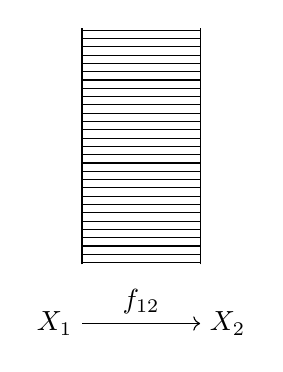
\begin{tikzpicture}[scale=0.75]
  \filldraw[draw=white,pattern=horizontal lines]
    (-1,1)
    rectangle
    (1,5);
  \draw
    (-1,1)
    --
    (-1,5);
  \draw
    (1,1)
    --
    (1,5);
  \draw[->]
    (-1,0)
    -- node[above] {$f_{12}$}
    (1,0);
  \draw
    (-1,0) node[left] {$X_{1}$}
    --
    (-1,0);
  \draw
    (1,0)
    --
    (1,0) node[right] {$X_{2}$};
\end{tikzpicture}
\]
and else
\[
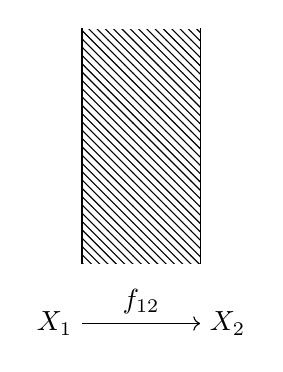
\begin{tikzpicture}[scale=0.75]
  \filldraw[draw=white,pattern=north west lines]
    (-1,1)
    rectangle
    (1,5);
  \draw
    (-1,1)
    --
    (-1,5);
  \draw
    (1,1)
    --
    (1,5);
  \draw[->]
    (-1,0)
    -- node[above] {$f_{12}$}
    (1,0);
  \draw
    (-1,0) node[left] {$X_{1}$}
    --
    (-1,0);
  \draw
    (1,0)
    --
    (1,0) node[right] {$X_{2}$};
\end{tikzpicture}
\]
hence a groupoid would be the special case when all arrows are illustrated by areas filled with horizontal paths. And, in fact, the guy in \cite{e5194763} concedes that philosophically $1$-arrows as in our approach to category theory are also legit as basic mathematical objects and do not necessarily have to be considered $1$-paths with additional structure. He even admits his line of argument as {\glqq}moot{\grqq} if somebody finds something such as UFP-HoTT for directed paths. That is, a formal synthetic theory of so-called {\glqq}directed homotopy theory{\grqq} - (synthetic) homotopy theory with directed $n$-paths, or $n$-arrows following our terminiological convention - as UFP-HoTT is (synthetic) homotopy theory with ordinary (undirected) $n$-paths. But at the moment UFP-HoTT is far more elaborated\footnote{indeed, it is almost mature enough to serve as a foundation of mathematics with basic mathematical objects $\infty$-groupoids} than any directed version of it. Which is another argument in \cite{e5194763} which we recommend as lazy weekend literature\footnote{it is no hard stuff} for the interested reader. By the way, the same author has written some quite worthwhile notes \cite{2d5c2e63} about intuition for homotopy type theory in a similar style we also want to recommend w.r.t. this subject.
\\\\
Now whatever we choose as higher-level set - higher groupoids or higher categories - we deal with weak versions of them and this suggests that equality should always be equivalence when talking about $N$-dimensional sets. This means (strict) equality on the $N$-th level and coherent isomorphism else unless $N = \infty$ where it just means coherent isomorphism. For sets this is equality and for $2$-dimensional sets it is isomorphism on $0$-morphisms and equality on $1$-morphisms. Note that if there was an $n+1$-st level then strict equality on the $n$-th level is identity. UFP-HoTT has a pretty nice perspective on this: identity isomorphisms are no better than coherent isomorphism, one just has to keep track which coherent isomorphism one took to prove equivalence. This is univalence and expresses that (strict) equality is expanded to equivalence. The modern approach to avoid this asymmetry of having both equality and isomorphisms in the categorical context is to consider $(N_{1},N_{2})$-categories which have arrows on all levels but all $k$-arrows with $k > N_{1} \geq N_{2}$ are identities and all $k$-arrows with $N_{1} \geq k > N_{2}$ are invertible. Equivalence is then just coherent isomorphism. In this setting $N$-categories are $(N,N)$-categories. $(N_{1},N_{2})$-categories are hybrids of $\infty$-groupoids and $\infty$-categories and might be used to find an $\infty$-category generalization of UFP-HoTT, where progress is made in the $(\infty,1)$-category case. $(\infty,1)$-categories are well-understood. You can imagine these as ordinary categories with the morphism sets not just $1$-dimensional sets but $\infty$-groupoids which is to say homotopy types by the Grothendieck hypothesis \ref{prp:groth}. This is needed when doing homotopy theory.\footnote{just think of fiber sequences in $\mathbf{Top}$, for example, where one has to topologize some morphism sets to make things work out} So $(\infty,1)$-categories provide a basic setting for doing homotopy theory. But we cannot expect this to suffice just like we couldn't expect set theory to work in any category equally well. There we found topos theory which provides a setting to do reasonable set theory. Therefore we would expect that a sensible notion of $(\infty,1)$-topoi is a setting for homotopy theory in that the objects of an $(\infty,1)$-topoi behave like homotopy types. This is, in fact, the case. However, we cannot further elaborate on that since we lack model categories as a $(1,1)$-categorical formulation of homotopy theory on the one hand and a formal definition of $(\infty,1)$-categories on the other. Moreover we lack some categorical ideas from later sections - fibrations (section \ref{sec:fibration}) and simplical sets (section \ref{sec:sset})- which are usually utilized in the formal definitions we would need. But let us already at this point refer to \cite{0349e8ea} to formally understand these things. In particular, the $(\infty,1)$-topos theory as the title of \cite{0349e8ea} suggests. \cite{0349e8ea} seems to be the undisputed standard reference on $(\infty,1)$-topoi theory. The internal language of $(\infty,1)$-topoi seems to be a homotopy type theory. Conclusively let us say that an $(\infty,1)$-topos is a place where one can do homotopy theory.
\\
Where we are at Lurie's work anyways, a historical remark: one of the main reasons to prefer $(N,N)$-categories over weak $N$-categories is that there are problems proving the so-called cobordism hypothesis due to Baez for the latter but Lurie proved it in case of $(\infty,N)$-categories. For more on this see \cite{ea5d49bf} and \cite{00000011}.
\\\\
After we have an idea what higher-level sets should be we turn to the question of how we can transfer structures on $N_{1}$-dimensional sets to according structures on $N_{2}$-dimensional sets.\footnote{a $0$-dimensional set can be seen as the truth values {\glqq}true{\grqq} and {\glqq}false{\grqq}} In particular, if we are given a method to transfer some sorts of structures on $N_{1}$-dimensional sets to according structures on $N_{2}$-dimensional sets then if the method is applied to a mere\footnote{without structure} $N_{1}$-dimensional set it should yield an $N_{2}$-dimensional set. This is a minimal condition for any sensible method and if it holds in the case $n_{2} = n_{1} + 1$ for all $n_{1},n_{2}$ we can construct - and hence define - $n$-dimensional sets for all $n$ by such a method.
\\
However this is not applicable directly to get $\infty$-dimensional sets and one has to rely on other methods. To get $\infty$-groupoids in UFP-HoTT, for example, the types\footnote{basic mathematical objects} are characterized by deductive steps which make all types behave like $\infty$-groupoids - or more intuitively: spaces. $n$-groupoids or better say $n$-types are then defined as the $\infty$-groupoids with only identities above level $n$. This allows to construct the $n+1$-groupoid/type of $n$-groupoids/types of some (univalent) universe\footnote{the idea is the same as for Grothendieck universes though UFP-HoTT uses Russell-style universes} $\mathcal{U}$ of types/$\infty$-groupoids as a subtype by a so-called dependent sum\footnote{something like a collection of ordered pairs where the second coordinate depends on the first} with first coordinate an inhabitant of the universe and the second a proof that this inhabitant is an $n$-groupoid/type. As a formula this looks like
\begin{align*}
  n\textrm{-Type}
  \doteq
  n\textrm{-Type}_{\mathcal{U}}
  &:=
  \sum_{T \colon \mathcal{U}}
  \textrm{is-}n\textrm{-type}(T)
\end{align*}
Let us agree that $\infty\textrm{-Type}_{\mathcal{U}}$ is just $\mathcal{U}$. Moreover there are rules for how to make the higher-groupoid structure of any $\infty$-groupoid trivial above some level $n$ to yield an $n$-groupoid. This is called $n$-truncation and corresponds to the $n$-th Postnikov section in classical homotopty theory with ordinary topological spaces. But unlike Postnikov towers in the classical sense $n$-truncation is formally built-in into UFP-HoTT. This is an important feature of UFP-HoTT. We could now hope to transfer higher-level structures by $n$-truncation. Namely assume a type $T$ and an $n$-type $T_{n}$ including some known structure, that is, the structure as part of the types. Then if $T_{n}$ is the $n$-truncation of $T$ and if the $n$-truncation has a right inverse - or better say is a section - then we would consider the type $T$ as a type with structure of the same sort as the structure on $T_{n}$. Note that $T$ can be a groupoid of any dimension and is not necessarily a non-trivial $\infty$-groupoid. But usually the dimension of $T$ is higher than $n$. We do not want to dig deeper at this point but rather turn to a process similar in spirit which also works very well. One might call it weak internalization:
\begin{description}
\item[Step 1]
define a structure on an inhabitant of $N\textrm{-Type}$ as something internal to $N\textrm{-Type}$ for some $N$
\item[Step 2]
try to use this internal definition for any $N$
\end{description}
For example one can define a (weak) $\infty$-group to be a (weak) group object of $\mathcal{U}$, then a weak $N$-group is a (weak) group object of the type of $N\textrm{-Type}_{\mathcal{U}}$. If you do not yet understand this you will after reading UFP-HoTT. But it is not so important for what follows. 
\\
One can think of similar ideas for $\infty$-categories if we have a serious definition of them at all.\footnote{at best a generalization of UFP-HoTT in the sense of a synthetic theory of directed homotopy theory} One can then again think of something like the $(n+1,n+1)$-category of $(n,n)$-categories ${}_{(n,n)}\mathbf{Cat}_{\mathcal{U}}$ where we agree to regard ${}_{(\infty,\infty)}\mathbf{Cat}_{\mathcal{U}}$ as a universe of $\infty$-categories. We can then hope to find an $n$-truncation which truncates an $\infty$-category to an $(n,n)$-category by making all arrows above level $n$-trivial. Hence we can hope to transfer higher-level structures by $n$-truncation corresponding to the higher groupoid case. Note that by $(\infty,n)$-categories we have a hybrid of $\infty$-groupoids and $\infty$-categories which suggests a weaker form of $n$-truncation such that an $\infty$-category is $n$-truncated to a an $(\infty,n)$-category by discarding all non-invertible arrows above level $n$. However, this shall not concern us here since the stronger notion is the one which corresponds to $n$-truncation in UFP-HoTT. And transferring higher-level structures by this strong $n$-truncation applies. In this way one can for example tranfer the structure of natural numbers on a set to the $1$-categorical context yielding $\mathbf{Finset}$. On the other hand, it is straight forward to generalize the idea of weak internalization as:
\begin{description}
\item[Step 1]
define a structure on an $N$-category as something internal to ${}_{(n,n)}\mathbf{Cat}$
\item[Step 2]
try to use this internal definition for any $N$
\end{description}
In subsection \ref{sec:internaliz} we got a taste of the importance of internalizaztion. So it is no surprise that weak internalization is at least as important: it is as least as good as internalization since it is internalization in the $(\infty,1)$-categorical context which is a generalization of category theory.
\\\\
If we are honest, the most likely case one encounters in practice is that one is given a structure on a set and wants to make sense of it in the $2$-dimensional set case. At best one hopes that this process is recursive and translates to a process to go from $n$ to $n+1$. Hence we want to generalize a structure on a set to a structure on a category or more general from the $n$ case to the $n+1$ case by an as of yet mostly informal algorithm which tells us how to do so. In the following we discuss two such ideas: (recursive) categorification\footnote{some people call it vertical categorification} and (recursive) oidification\footnote{some people call it horizontal categorification}.\footnote{the word recursive is not part of the standard terminology but we find it less confusing at this point since transferring higher-level structures by $n$-truncation and weak internalization are also considered a kind of categorification where we avoid the terminology, too}
\\
But let us first reconsider how the dimension terminology of higher-level sets emerges if we want $n+1$-dimensional sets to be $n$-categories. What we mean is that a set is just an unstructured collection but a category $\mathbf{C}$ consists essentially of a set of objects $\mathrm{ob}_{\mathbf{C}}$ and a set of arrows $\mathrm{Mor}_{\mathbf{C}}$ (governed by composition) - a $2$-tuple - while a $3$-category consists of a set of $0$-arrows (objects), a set of $1$-arrows (morphisms) and a set of $2$-arrows (governed by two kinds of composition: vertical and horizontal) - a $3$-tuple. This process extends to an arbitrary $n$ (provided we have a definition of $n$-category). It is these $n$-tuples we mean when we say set of dimension $n$. Moreover, note that a functor is a $2$-dimensional function in this sense since it essentially consists of two functions - one on objects and one on morphisms. And an $N$-functor between $N$-categories should be just like functions $f_{n^{\backprime}}$ where $n^{\backprime} \in \mathbb{N}_{N}$ such that $f_{n^{\backprime}}$ maps $n^{\backprime}$-morphism to $n^{\backprime}$-morphisms respecting the various compositions and identities in a weak way, that is, up to equuivalence.\footnote{one also gets coherence conditions for $n$-functors}. Moreover note that a natural transformation is a function mapping $0$-morphisms to $1$-morphisms respecting the functor application.\footnote{it doesn't matter if we first apply the functor and then transform or the other way around} In the $N$-category case this suggests to consider $N$-functors and $N$-natural transformations as special cases of a more general notion called transfor\footnote{made-up word from functor and natural transformation}. Let $n_{0} \in \mathbb{N}_{N}^{\times}$ then if $(N,n_{0}-1)$-transfor is defined, an $(N,n_{0})$-transfor should be a family of functions indexed by $n^{\backprime} \leq N - n_{0}$ mapping $n^{\backprime}$-morphisms to $n^{\backprime}+n_{0}$-morphisms respecting $(N,n_{0}-1)$-transfor application up to equivalence where the $(N,0)$-transfor case should be just an $N$-functor. $(N,1)$-transfors shall then be $N$-natural transformations. Let us illustrate this a bit for $N \neq \infty$. If
\[
\begin{tikzcd}[sep=tiny]
  {}_{0}\mathrm{Mor}_{\mathbf{W}}
  \\
  \vdots
  \\
  {}_{n}\mathrm{Mor}_{\mathbf{W}}
\end{tikzcd}
\]
illustrates an $n$-category $\mathbf{W}$, then for $n$-categories $\mathbf{W}_{1}$ and $\mathbf{W}_{2}$ we can illustrate an $(n,n_{0})$-transfor for $n-n_{0}$ large enough as
\[
\begin{tikzcd}[row sep=tiny,column sep=large]
  {}_{0}\mathrm{Mor}_{\mathbf{W}_{1}}
  \arrow{rdd}{}
  &
  {}_{0}\mathrm{Mor}_{\mathbf{W}_{2}}
  \\
  \vdots
  &
  \vdots
  \\
  {}_{n_{0}}\mathrm{Mor}_{\mathbf{W}_{1}}
  \arrow{rdd}{}
  &
  {}_{n_{0}}\mathrm{Mor}_{\mathbf{W}_{2}}
  \\
  \vdots
  &
  \vdots
  \\
  \vdots
  &
  {}_{n_{0}+n_{0}}\mathrm{Mor}_{\mathbf{W}_{2}}
  \\
  \vdots
  &
  \vdots
  \\
  {}_{n-n_{0}}\mathrm{Mor}_{\mathbf{W}_{1}}
  \arrow{rdd}{}
  &
  \vdots
  \\
  \vdots
  &
  \vdots
  \\
  {}_{n}\mathrm{Mor}_{\mathbf{W}_{1}}
  &
  {}_{n}\mathrm{Mor}_{\mathbf{W}_{2}}
\end{tikzcd}
\]
The up to equivalencs part cannot be illustrated here in generality. The coherence laws are way to complicated for our means. But we saw a special case in subsection \ref{sec:nt} and we will see some more in subsubsection \ref{sec:hlm}.
\\
We now come to the categorification and oidification.
\begin{enumerate}
\item[(RC)]
Categorification is the following as of yet mostly informal process: for all $n$ when given a bunch of $n$-categories and a bunch of $(n,n_{0})$-transfors for all $0 \leq n_{0} \leq n$ subjected to some conditions only involving the $n$-categories and $(n,n_{0})$-transfors - this can be seen as a structure on these $n$-categories - then by replacing
\begin{description}
\item[Step 1]
each $n$-category by an $n+1$-category
\item[Step 2]
each $(n,n_{0})$-transfor by a suited $(n+1,n_{0})$-transfor
\end{description}
we have categorified the structure to $n+1$-categories. A more thorough discussion of this is given in \cite{66edf75b}. Let us emphasize what this means when categorifying a set: given a bunch of sets and a bunch of functions with both domain and codomain involving only these sets subjected to some conditions involving only these sets and functions then we can replace each set by a category and each function by a suited functor (the $(1,0)$-transfors). In particular, an equality of sets must be replaced by equivalence (what actually should have aready been done earlier) and equality of function by equivalence (the $(1,1)$-transfors up to coherent isomorphism).
\\
An example is to categorify a monoid $(M,\cdot,\mathrm{id})$. We replace $M$ by a category $\mathbf{C}$ and $\cdot$ by a functor from $\mathbf{C} \times \mathbf{C}$ to $\mathbf{C}$ as well as $\mathrm{id}$ by a functor from $\mathbf{1}_{M}$ to $\mathbf{C}$ which by the terminality of $\mathbf{1}_{M}$ in $\mathbf{Cat}$ is nothing but an object $1$ of $\mathbf{C}$. In the monoid properties (M1) and (M2) we replace $=$ by natural isomorphism. Then one has to look at the result what is missing to make it a sensible conception. We do this in subsubsection \ref{sec:hlm} and categorify a monoid to a monoidal category. An interesting peculiarity is that one can internalize monoids in monoidal categories. This is a further idea which is called microcosm principle coined by Baez and Dolan in \cite{0d7b89ad} where they give a definition of weak $n$-category and prove a version of the microcosm principle which says that when we categorify a structure we can internalize this structure there. Though as already mentioned weak $n$-categories are not used much anymore due to their addressed drawback, the paper \cite{0d7b89ad} is a seminal one on higher categories and does still provide good intuition. So we can still recommend reading it.
\item[(RO)]
Actually, we have already introduced the informal meta-idea of oidification on the quiet by two examples earlier in the notes. Namely the oidification of a monoid is a category while the oidification of a group is a groupoid. The process in these cases was that we had a structure on a set (monoid and group) and could show that it is equivalent to a certain kind of category (ordinary category and category with only isomorphisms, respectively) with exactly one object. Then we allowed the kind of the category to contain arbitrarily many objects to complete the oidification of the structure on a set. So oidification in higher category theory should be very much like categorification: take a structure on an $n$-category and transfer it to the next level. Hence oidification is described by the following meta-algorithm: Given some structure on an $n$-category for some $n \in \mathbb{N}$ then
\begin{description}
\item[Step 1]
show that the structure on this $n$-category is equivalent to a certain kind of $n+1$-category with precisely one $0$-morphism
\item[Step 2]
oidify by passing to this certain kind of $n+1$-category but allow arbitrarily many $0$-morphisms
\end{description}
\end{enumerate}
In the end, one might recognize that recursive categorification and oidification also allows to go from finite $n$ directly to $\infty$ after all. That it is presented recursively is arguably for historical reasons.
\\\\
All in all this subsection suggests that the $\infty$-version of structure is more fundamental than any finite version in the sense that the $\infty$-dimensional sets are the basic mathematical object rather than just ordinary sets.
\\
The following subsection applies many of the ideas sketched here in case of monoids yielding mostly formal definitions.

\subsubsection{Higher-Level Monoid}
\label{sec:hlm}
%\nocite{24253327}
%\nocite{0d7b89ad}
%\nocite{c2d89e8a}
%\nocite{de09a3f9}
\nocite{bc53e62a}
%\nocite{00000011}
%TODO
%  cite somthing understadable for coherence and strictification
%  more on operads
%  monadicity theorem
In this subsubsection we categorify monoids with the method described earlier in this subsection to get the notion of monoidal category. Subsequently, it turns out that that we can define functors and natural transformations preserving the monoidal structure. We then do the same when the monoid is commutative. After this we look at an example regarding vector spaces before generalizing category theory to enriched category theory. From all this it will become quite clear that we can internalize monoids in monoidal categories and this will be utilized to define monads as oidification of monoid objects in monoidal categories. The original case of monads is the case $\mathbf{Cat}$. An even more special case is the restriction to a certain category of set-valued functors we allude to and provide references for. The monoidal objects there are operads\footnote{a word built from operation an monad} which were developed by May (among others) to study iterated loop spaces which can be used to define the homotopy groups and are hence of interest regarding the coherence conditions for higher categories
\\
But be warned that the discussion in this subsubsection is mostly superficial and we mostly provide only terminology. Unfortunately, we do not have the time (and means) here to prove any deep theorems like coherence theorems or the strictification theorem. We only provide the bare necessities needed to delve into the literaure we refer to.
\\\\
But now back to the salt mines. A set $\mathcal{M}_{\mathbf{C}}$ is a \textbf{monoidal category} if it is a $6$-tuple
\begin{align*}
  \left(
    \mathbf{C},
    \otimes,
    \mathsf{A},
    1,
    \mathsf{L},
    \mathsf{R}
  \right)
\end{align*}
consisting of
\begin{enumerate}
\item[(1)]
a category $\mathbf{C}$
\item[(2)]
a functor
\begin{align*}
  \cdot
  \otimes
  \cdot
  \doteq
  \otimes
  \colon
  \mathbf{C}
  \times
  \mathbf{C}
  &\rightarrow
  \mathbf{C}
\end{align*}
\item[(3)]
for the functors
\begin{align*}
  \left(
    \cdot
    \otimes
    \cdot
  \right)
  \otimes
  \cdot
  \doteq
  {}_{\otimes}\otimes
  \colon
  \mathbf{C}
  \times
  \mathbf{C}
  \times
  \mathbf{C}
  &\rightarrow
  \mathbf{C}
  \\
  (X_{1},X_{2},X_{3})
  &\mapsto
  \otimes(\otimes(X_{1},X_{2}),X_{3})
  \\
  (f_{12},f_{34},f_{56})
  &\mapsto
  \otimes(\otimes(f_{12},f_{34}),f_{56})
  \\\\
  \cdot
  \otimes
  \left(
    \cdot
    \otimes
    \cdot
  \right)
  \doteq
  \otimes_{\otimes}
  \colon
  \mathbf{C}
  \times
  \mathbf{C}
  \times
  \mathbf{C}
  &\rightarrow
  \mathbf{C}
  \\
  (X_{1},X_{2},X_{3})
  &\mapsto
  \otimes(X_{1},\otimes(X_{2},X_{3}))
  \\
  (f_{12},f_{34},f_{56})
  &\mapsto
  \otimes(f_{12},\otimes(f_{34},f_{56}))
\end{align*}
a natural isomorphism
\begin{align*}
  \mathsf{A}
  \colon
  {}_{\otimes}\otimes
  &\Rightarrow
  \otimes_{\otimes}
\end{align*}
\item[(4)]
an object\footnote{don't mix this up with terminal objects since it is just an unfortunate notational coincidence as so often is the case for this symbol} $1$ of $\mathrm{ob}_{\mathbf{C}}$
\item[(5)]
for the functor
\begin{align*}
  \otimes(1,\cdot)
  \colon
  \mathbf{C}
  &\rightarrow
  \mathbf{C}
  \\
  X
  &\mapsto
  \otimes(1,X)
  \\
  f_{12}
  &\mapsto
  \otimes(\mathrm{id}_{1},f_{12})
\end{align*}
a natural isomorphism
\begin{align*}
  \mathsf{L}
  \otimes(1,\cdot)
  \colon
  &\Rightarrow
  \mathrm{id}_{\mathbf{C}}
\end{align*}
\item[(6)]
for the functor
\begin{align*}
  \otimes(\cdot,1)
  \colon
  \mathbf{C}
  &\rightarrow
  \mathbf{C}
  \\
  X
  &\mapsto
  \otimes(X,1)
  \\
  f_{12}
  &\mapsto
  \otimes(f_{12},\mathrm{id}_{1})
\end{align*}
a natural isomorphism
\begin{align*}
  \mathsf{R}
  \colon
  \otimes(\cdot,1)
  &\Rightarrow
  \mathrm{id}_{\mathbf{C}}
\end{align*}
\end{enumerate}
such that
\begin{enumerate}
\item[(MC1)]
the diagram
\[
\begin{tikzcd}[row sep=3.5em,column sep=0.4em]
  &
  (X_{1} \otimes X_{2})
  \otimes
  (X_{3} \otimes X_{4})
  \arrow{dr}{\mathsf{A}(X_{1},X_{2},X_{3} \otimes X_{4})}
  &
  \\
  \left(
    (X_{1} \otimes X_{2})
    \otimes
    X_{3}
  \right)
  \otimes
  X_{4}
  \arrow{ur}{\mathsf{A}(X_{1} \otimes X_{2},X_{3},X_{4})}
  \arrow[swap]{d}{\mathsf{A}(X_{1},X_{2},X_{3}) \otimes \mathrm{id}_{X_{4}}}
  &
  &
  X_{1}
  \otimes
  \left(
    X_{2}
    \otimes
    (X_{3} \otimes X_{4})
  \right)
  \\
  \left(
    X_{1}
    \otimes
    (X_{2} \otimes X_{3})
  \right)
  \otimes
  X_{4}
  \arrow{rr}{\mathsf{A}(X_{1},X_{2} \otimes X_{3},X_{4})}
  &
  &
  X_{1}
  \otimes
  \left(
    (X_{2} \otimes X_{3})
    \otimes
    X_{4}
  \right)
  \arrow[swap]{u}{\mathrm{id}_{X_{1}} \otimes \mathsf{A}(X_{2},X_{3},X_{4})}
\end{tikzcd}
\]
commutes
\item[(MC2)]
the diagram
\[
\begin{tikzcd}[sep=large]
  (X_{1} \otimes 1)
  \otimes
  X_{2}
  \arrow{rr}{\mathsf{A}(X_{1},1,X_{2})}
  \arrow[swap]{dr}{\mathsf{R}(X_{1}) \otimes \mathrm{id}_{X_{2}}}
  &
  &
  X_{1}
  \otimes
  (1 \otimes X_{2})
  \arrow{dl}{\mathrm{id}_{X_{1}} \otimes \mathsf{L}(X_{2})}
  \\
  &
  X_{1}
  \otimes
  X_{2}
  &
\end{tikzcd}
\]
commutes
\end{enumerate}
The sets given by the coordinates of a monoidal category
\begin{align*}
  \mathbf{C}
  \doteq
  \mathcal{M}_{\mathbf{C}}
  &=
  \left(
    \mathbf{C},
    \otimes,
    \mathsf{A},
    1,
    \mathsf{L},
    \mathsf{R}
  \right)
\end{align*}
have names in their own right.
\begin{enumerate}
\item[(1)]
$\mathbf{C}$ is called the \textbf{underlying category (in $\mathcal{M}_{\mathbf{C}}$)}
\item[(2)]
$\otimes$ is called the \textbf{tensor product (in $\mathcal{M}_{\mathbf{C}}$)}
\item[(3)]
$\mathsf{A}$ is called the \textbf{associator (in $\mathcal{M}_{\mathbf{C}}$)}
\item[(4)]
$1$ is called the \textbf{unit object (in $\mathcal{M}_{\mathbf{C}}$)}
\item[(5)]
$\mathsf{L}$ is called the \textbf{left unit law (in $\mathcal{M}_{\mathbf{C}}$)}
\item[(6)]
$\mathsf{R}$ is called the \textbf{right unit law (in $\mathcal{M}_{\mathbf{C}}$)}
\end{enumerate}
For the monoidal category property (MC1) we also say that the \textbf{pentagon equation (in $\mathcal{M}_{\mathbf{C}}$) holds} whereas we say for the monoidal category property (MC2) that the \textbf{triangle equation (in $\mathcal{M}_{\mathbf{C}}$) holds}. The pentagon equation is the coherence condition for associativity of weak $2$-categories we already talked about in subsection \ref{sec:nt}. That this suffices is Mac Lane's coherence theorem which can be found in his category book \cite{e837ef86} or various other sources. The triangle equation is the identity law counterpart, that is, the coherence condition for the identity law which can also be found in \cite{e837ef86} or various other sources. Hence the pentagon and tirangle equation make monoidal category a sensible (weak\footnote{if we only wanted to categorify it strictly we would not need them}) categorification of monoid. The relation to weak $2$-categories should be clear from this - at least if one keeps in mind the different notational conventions for composition and tensor product (the arguments are in reversed order): monoidal categories correspond to the weak $2$-categories with precisely one object (in anology to monoids corresponding to ordinary categories with precisely one object). Hence weak $2$-categories are the oidification of monoidal categories (as categories are the oidification of monoids). One might expect this to continue and so it is. But this is another story not told here. What is interesting  to us here is that we directly get examples for monoidal categories from the examples of weak $2$-categories we already know since for a weak $2$-category ${}_{2}\mathbf{C}$ (in the notation we used in the definition of the concept) we get for all
\begin{align*}
  X
  \in
  {}_{0}\mathrm{mor}_{{}_{2}\mathbf{C}}
\end{align*}
a monoidal category
\begin{align*}
  \left(
    {}_{1}\mathbf{mor}_{{}_{2}\mathbf{C}}(X,X),
    \circ^{\textrm{h}}(X,X,X),
    \mathsf{A}(X,X,X),
    \mathrm{id}_{X},
    \mathsf{L}(X),
    \mathsf{R}(X)
  \right)
\end{align*}
Now, well, we do not know many examples but we could consider ${}_{2}\mathbf{Cat}$ as weak $2$-category with associators and unitors just identities. In this case, the monoidal categories are the functor categories $\mathbf{C}^{\mathbf{C}}$ for any small $\mathbf{C}$ which some people call category of endofunctors. Let us write
\begin{align*}
  \mathrm{end}(\mathbf{C})
  &:=
  {}_{1}\mathbf{mor}_{{}_{2}\mathbf{Cat}}(\mathbf{C},\mathbf{C})
\end{align*}
for this monoidal category.
\\
The next point are monoidal functors. A set $\mathcal{M}_{F}$ is a \textbf{lax monoidal functor (from $\mathcal{M}_{\mathbf{C}}$ to $\mathcal{M}_{\mathbf{C}_{\alpha}}$)} if it is a $3$-tuple
\begin{align*}
  F
  \doteq
  \left(
    F,
    \mathsf{H},
    \Phi
  \right)
\end{align*}
consisting of a functor $F$ from $\mathbf{C}$ to $\mathbf{C}_{\alpha}$, a natural transformation
\begin{align*}
  \mathsf{H}
  \colon
  \otimes_{\alpha}
  \circ
  \left(
    F
    \times
    F
  \right)
  &\Rightarrow
  F
  \circ
  \otimes
\end{align*}
and an morphism
\begin{align*}
  \Phi
  &\in
  \mathrm{mor}_{\mathbf{C}_{\alpha}}(1_{\alpha},F(1))
\end{align*}
such that
\begin{enumerate}
\item[(MF1)]
the diagram
\[
\begin{tikzcd}[row sep=3em, column sep=9em]
  (F(X_{1}) \otimes_{\alpha} F(X_{2}))
  \otimes_{\alpha}
  F(X_{3})
  \arrow{r}{\mathsf{A}_{\alpha}(F(X_{1}),F(X_{2}),F(X_{3}))}
  \arrow[swap]{d}{\mathsf{H}(X_{1},X_{2})\otimes_{\alpha}\mathrm{id}_{F(X_{3})}}
  &
  F(X_{1})
  \otimes_{\alpha}
  (F(X_{2}) \otimes_{\alpha} F(X_{3}))
  \arrow{d}{\mathrm{id}_{F(X_{1})} \otimes_{\alpha} \mathsf{H}(X_{2},X_{3})}
  \\
  F(X_{1} \otimes X_{2})
  \otimes_{\alpha}
  F(X_{3})
  \arrow[swap]{d}{\mathsf{H}(X_{1} \otimes X_{2},X_{3})}
  &
  F(X_{1})
  \otimes_{\alpha}
  F(X_{2} \otimes X_{3})
  \arrow{d}{\mathsf{H}(X_{1},X_{2} \otimes X_{3})}
  \\
  F
  \left(
    (X_{1} \otimes X_{2})
    \otimes
    X_{3}
  \right)
  \arrow{r}{F(\mathsf{A}(X_{1},X_{2},X_{3}))}
  &
  F
  \left(
    X_{1}
    \otimes
    (X_{2} \otimes X_{3})
  \right)
\end{tikzcd}
\]
commutes
\item[(MF2)]
the diagrams
\[
\begin{tikzcd}[sep=large]
  1_{\alpha}
  \otimes_{\alpha}
  F(X)
  \arrow{r}{\mathsf{L}_{\alpha}(F(X))}
  \arrow[swap]{d}{\Phi \otimes_{\alpha} \mathrm{id}_{F(X)}}
  &
  F(X)
  \\
  F(1)
  \otimes_{\alpha}
  F(X)
  \arrow{r}{\mathsf{H}(1,X)}
  &
  F(1 \otimes X)
  \arrow[swap]{u}{F(\mathsf{L}(X))}
\end{tikzcd}
\]
and
\[
\begin{tikzcd}[sep=large]
  F(X)
  \otimes_{\alpha}
  1_{\alpha}
  \arrow{r}{\mathsf{R}_{\alpha}(F(X))}
  \arrow[swap]{d}{\mathrm{id}_{F(X)} \otimes_{\alpha} \Phi}
  &
  F(X)
  \\
  F(X)
  \otimes_{\alpha}
  F(1)
  \arrow{r}{\mathsf{H}(X,1)}
  &
  F(X \otimes 1)
  \arrow[swap]{u}{F(\mathsf{R}(X))}
\end{tikzcd}
\]
commute
\end{enumerate}
Furthermore monoidal functor properties (MF1) and (MF2) express that the functor $F$ is compatible with the according monoidal structures as coherence condition. A lax monoidal functor $(F,\mathsf{H},\Phi)$ is called\footnote{some use strong monoidal functor here but we don't since this is our standard case} \textbf{monoidal functor} if both $\mathsf{H}$ and $\Phi$ are isomorphisms while it is called \textbf{strict monoidal functor} if both are identities. It is clear that
\begin{align*}
  \left(
    \mathrm{id}_{\mathbf{C}},
    \mathrm{id}_{\mathrm{id}_{\mathbf{C}}},
    \mathrm{id}_{1}
  \right)
\end{align*}
is a monoidal functor if $\mathcal{M}_{\mathbf{C}}$ is a monoidal category. Checking the axioms is straightforward and therefore omitted. A little more tedious - above all with respect to notation - is the proof that
\begin{align*}
  \left(
    F_{\beta\gamma}
    \circ
    F_{\alpha\beta},
    F_{\beta\gamma}
    \left(
      \mathsf{H}_{\alpha\beta}(\cdot,\cdot)
    \right)
    \circ
    \mathsf{H}_{\beta\gamma}
    \left(
      \left(
        F_{\alpha\beta}
        \times
        F_{\alpha\beta}
      \right)
      (\cdot,\cdot)
    \right),
    \Phi_{\beta\gamma}
    \circ
    \Phi_{\alpha\beta}
  \right)
\end{align*}
is a monoidal functor if
\begin{align*}
  \left(
    F_{\alpha\beta},
    \mathsf{H}_{\alpha\beta},
    \Phi_{\alpha\beta}
  \right)
  \qquad
  &\text{and}
  \qquad
  \left(
    F_{\beta\gamma},
    \mathsf{H}_{\beta\gamma},
    \Phi_{\beta\gamma}
  \right)
\end{align*}
are monoidal functors. So let us forgo the proof here, too. After all, it is clear what the category of small monoidal categories $\mathbf{MonCat}$ shall be. That this is actually a (strict) $2$-category comes now.
\\
One can strightforwardly guess that if there are notions of monoidal category and monoidal functor there is also a notion of monoidal natural transformation. Indeed, there is one and it turns out that not much is required for natural transformations to be monoidal, that is, to get along with the monoidal structures. Given monoidal functors
\begin{align*}
  \left(
    F_{1},
    \mathsf{H}_{1},
    \Phi_{1}
  \right)
  \qquad
  &\text{and}
  \qquad
  \left(
    F_{2},
    \mathsf{H}_{2},
    \Phi_{2}
  \right)
\end{align*}
a natural transformation $\mathsf{T}_{12}$ is \textbf{monoidal (w.r.t $\mathcal{M}_{F_{1}}$ and $\mathcal{M}_{F_{2}}$)} if
\begin{enumerate}
\item[(MT1)]
the diagram
\[
\begin{tikzcd}[row sep=large,column sep=8em]
  F_{1}(X_{1})
  \otimes_{\alpha}
  F_{1}(X_{2})
  \arrow{r}{\mathsf{T}_{12}(X_{1}) \otimes_{\alpha} \mathsf{T}_{12}(X_{2})}
  \arrow[swap]{d}{\mathsf{H}_{1}(X_{1},X_{2})}
  &
  F_{2}(X_{1})
  \otimes_{\alpha}
  F_{2}(X_{2})
  \arrow{d}{\mathsf{H}_{2}(X_{1},X_{2})}
  \\
  F_{1}(X_{1} \otimes X_{2})
  \arrow{r}{\mathsf{T}_{12}(X_{1} \otimes X_{2})}
  &
  F_{2}(X_{1} \otimes X_{2})
\end{tikzcd}
\]
commutes
\item[(MT2)]
the diagram
\[
\begin{tikzcd}[sep=large]
  1_{\alpha}
  \arrow{dr}{\Phi_{2}}
  \arrow{d}[swap]{\Phi_{1}}
  &
  \\
  F_{1}(1)
  \arrow{r}{\mathsf{T}_{12}(1)}
  &
  F_{2}(1)
\end{tikzcd}
\]
commutes
\end{enumerate}
Again the monoidal natural transformation properties (MT1) and (MT2) apparently express compatibility regarding the involved structures and are hence coherence conditions. One is now tempted to define a version of functor equivalence which is adapted to the new situation, that is, which respects the monoidal structure. Since the identity functor and the composition of functors are monoidal, all we have to do to achieve this is to add the word monoidal in the definition of equivalence: $\mathcal{M}_{F_{\alpha\beta}}$ is a \textbf{monoidal equivalence (from $\mathcal{M}_{\mathbf{C}_{\alpha}}$ to $\mathcal{M}_{\mathbf{C}_{\beta}}$)} if there is $\mathcal{M}_{F_{\beta\alpha}}$ such that there exist monoidal natural isomorphisms from $F_{\beta\alpha} \circ F_{\alpha\beta}$ to $\mathrm{id}_{\mathbf{C_{\alpha}}}$ and from $F_{\alpha\beta} \circ F_{\beta\alpha} $ to $\mathrm{id}_{\mathbf{C_{\beta}}}$, respectively. Thus we get the correct idea of when two monoidal categories are {\glqq}the same{\grqq} in the higher structural setting.
\\\\
As in abstract algebra a monoid can satisfy a commutative law and so can a monoidal category in a somewhat weaker form. This is braiding - or a little stronger - symmetry on a monoidal category. As the name suggests it is inspired by \textit{braids} in algebraic topology. However, we only provide the categorical basics for braids here. A set $\mathcal{B}_{\mathbf{C}}$ is a \textbf{braided monoidal category} if it is a tuple $(\mathcal{M}_{\mathbf{C}},\mathsf{B})$ consisting of a monoidal category $\mathcal{M}_{\mathbf{C}}$ and for the functor
\begin{align*}
  \otimes_{\textrm{B}}
  \colon
  \mathbf{C}
  \times
  \mathbf{C}
  &\rightarrow
  \mathbf{C}
  \\
  (X_{1},X_{2})
  &\mapsto
  \otimes(X_{2},X_{1})
  \\
  (f_{12},f_{34})
  &\mapsto
  \otimes(f_{34},f_{12})
\end{align*}
a natural isomorphism
\begin{align*}
  \mathsf{B}
  \colon
  \otimes
  &\Rightarrow
  \otimes_{\textrm{B}}
\end{align*}
such that
\begin{enumerate}
\item[(BC1)]
the diagram
\[
\begin{tikzcd}[row sep=huge,column sep=8em]
  (X_{2} \otimes X_{1})
  \otimes
  X_{3}
  \arrow{r}{\mathsf{A}(X_{2},X_{1},X_{3})}
  &
  X_{2}
  \otimes
  (X_{1} \otimes X_{3})
  \arrow{d}{\mathrm{id}_{X_{2}} \otimes \mathsf{B}(X_{1},X_{3})}
  \\
  (X_{1} \otimes X_{2})
  \otimes
  X_{3}
  \arrow{u}{\mathsf{B}(X_{2},X_{1}) \otimes \mathrm{id}_{X_{3}}}
  &
  X_{2}
  \otimes
  (X_{3} \otimes X_{1})
  \arrow{d}{\mathsf{A}^{-1}(X_{2},X_{3},X_{1})}
  \\
  X_{1}
  \otimes
  (X_{2} \otimes X_{3})
  \arrow{u}{\mathsf{A}^{-1}(X_{1},X_{2},X_{3})}
  \arrow{r}{\mathsf{B}(X_{1},X_{2} \otimes X_{3})}
  &
  (X_{2} \otimes X_{3})
  \otimes
  X_{1}
\end{tikzcd}
\]
commutes
\item[(BC2)]
the diagram
\[
\begin{tikzcd}[row sep=huge,column sep=8em]
  X_{1}
  \otimes
  (X_{3} \otimes X_{2})
  \arrow{r}{\mathsf{A}^{-1}(X_{1},X_{3},X_{2})}
  &
  (X_{1} \otimes X_{3})
  \otimes
  X_{2}
  \arrow{d}{\mathsf{B}(X_{1},X_{3}) \otimes \mathrm{id}_{X_{2}}}
  \\
  X_{1}
  \otimes
  (X_{2} \otimes X_{3})
  \arrow{u}{\mathrm{id_{X_{1}}} \otimes \mathsf{B}(X_{2},X_{3})}
  &
  (X_{3} \otimes X_{1})
  \otimes
  X_{2}
  \arrow{d}{\mathsf{A}(X_{3},X_{1},X_{2})}
  \\
  (X_{1} \otimes X_{2})
  \otimes
  X_{3}
  \arrow{u}{\mathsf{A}(X_{1},X_{2},X_{3})}
  \arrow{r}{\mathsf{B}(X_{1} \otimes X_{2},X_{3})}
  &
  X_{3}
  \otimes
  (X_{1} \otimes X_{2})
\end{tikzcd}
\]
commutes
\end{enumerate}
For the braided monoidal category properties (BC1) and (BC2) we also say that the \textbf{hexagon equations (in $\mathcal{B}_{\mathbf{C}}$) hold}. This is again a coherence condition. Often people only mention the underlying category of the monoidal category when they mean a braided monoidal category letting the rest of the data be implicit. The coordinate $\mathsf{B}$ in $\mathcal{B}_{\mathbf{C}}$ is called \textbf{braiding} and there is a case of special interest. Namely, a braided monoidal category $\mathcal{B}_{\mathbf{C}}$ is \textbf{symmetric} if
\begin{align*}
  \mathsf{B}(X_{2},X_{1})
  \circ
  \mathsf{B}(X_{1},X_{2})
  &=
  \mathrm{id}_{\otimes}(X_{1},X_{2})
\end{align*}
holds for all $X_{1}$ and $X_{2}$.\footnote{by the way, this equation is abstracted from a trivial braid}. People often say a bit inaccurately {\glqq}symmetric monoidal category{\grqq} instead of {\glqq}symmetric braided monoidal category{\grqq}.
\\
Of course, one can define functors respecting these extra pieces of structure. A set $\mathcal{B}_{F}$ is a \textbf{braided monoidal functor (from $\mathcal{B}_{\mathbf{C}}$ to $\mathcal{B}_{\mathbf{C}_{\alpha}}$)} if it is a monoidal functor $(F,\mathsf{H},\Phi)$ such that
\begin{enumerate}
\item[(BF)]
the diagram
\[
\begin{tikzcd}[row sep=large,column sep=8em]
  F(X_{1})
  \otimes_{\alpha}
  F(X_{2})
  \arrow{r}{\mathsf{B}_{\alpha}(F(X_{1}),F(X_{2}))}
  \arrow[swap]{d}{\mathsf{H}(X_{1},X_{2})}
  &
  F(X_{2})
  \otimes_{\alpha}
  F(X_{1})
  \arrow{d}{\mathsf{H}(X_{2},X_{1})}
  \\
  F(X_{1} \otimes X_{2})
  \arrow{r}{F(\mathsf{B}(X_{1},X_{2}))}
  &
  F(X_{2} \otimes X_{1})
\end{tikzcd}
\]
commutes
\end{enumerate}
Let us consider the symmetric case. As a special case of braiding there are clearly no extra conditions required for functors except for a restriction to symmetric monoidal categories.\footnote{so, if at all, axiom (BF) simplifies} Therefore a braided monoidal functor $\mathcal{B}_{F_{1}}$ is \textbf{symmetric} if
\begin{align*}
  \mathsf{B}(X_{2},X_{1})
  \circ
  \mathsf{B}(X_{1},X_{2})
  &=
  \mathsf{id}_{\otimes}(X_{1},X_{2})
  \\
  \mathsf{B_{\alpha}}(X_{2},X_{1})
  \circ
  \mathsf{B_{\alpha}}(X_{1},X_{2})
  &=
  \mathsf{id}_{\otimes_{\alpha}}(X_{1},X_{2})
\end{align*}
hold. That is, the involved categories are symmetric. Again, people say a bit inaccurately {\glqq}symmetric monoidal functor{\grqq} instead of {\glqq}symmetric braided monoidal functor{\grqq}. Once more, it is clear that
\begin{align*}
  \left(
    \mathrm{id}_{\mathbf{C}},
    \mathrm{id}_{\mathrm{id}_{\mathbf{C}}},
    \mathrm{id}_{1}
  \right)
\end{align*}
is a braided monoidal functor if $\mathsf{B}_{\mathbf{C}}$ is a braided monoidal category. Checking the axioms is straightforward and therefore omitted. Just a little more tedious - again for notational reasons - is the proof that
\begin{align*}
  \left(
    F_{\beta\gamma}
    \circ
    F_{\alpha\beta},
    F_{\beta\gamma}
    \left(
      \mathsf{H}_{\alpha\beta}(\cdot,\cdot)
    \right)
    \circ
    \mathsf{H}_{\beta\gamma}
    \left(
      \left(
        F_{\alpha\beta}
        \times
        F_{\alpha\beta}
      \right)
      (\cdot,\cdot)
    \right),
    \Phi_{\beta\gamma}
    \circ
    \Phi_{\alpha\beta}
  \right)
\end{align*}
is a braided monoidal functor if
\begin{align*}
  \left(
    F_{\alpha\beta},
    \mathsf{H}_{\alpha\beta},
    \Phi_{\alpha\beta}
  \right)
  \qquad
  &\text{and}
  \qquad
  \left(
    F_{\beta\gamma},
    \mathsf{H}_{\beta\gamma},
    \Phi_{\beta\gamma}
  \right)
\end{align*}
are braided monoidal functors. So let's forgo the proof here once more. In particular, we can replace braided by symmetric and the statements about the identity and composition will still hold. Again, it is clear what the category of small braided monoidal categories $\mathbf{BMonCat}$ and symmetric braided monoidal categories $\mathbf{SMonCat}$, respectively, shall be. That both of them are actually a (strict) $2$-category comes now.
\\
We wonder what we have to demand for naturality in case of braided monoidal functors. The answer is: actually nothing since the braiding as natural transformation between functors does not make use of the braided monoidal functors we want to define a certain kind of natural transformation for. So we are led to the definition that a natural transformation is \textbf{braided monoidal (w.r.t. $\mathcal{B}_{F_{1}}$ and $\mathcal{B}_{F_{2}}$)} if it is monoidal w.r.t. $\mathcal{B}_{F_{1}}$ and $\mathcal{B}_{F_{2}}$. To shine a light on the perhaps a little obscured part of this definition: the difference between braided monoidal and mere monoidal natural transformations is that the involved functors are braided monoidal and not just monoidal. Obtaining the symmetric monoidal case from the braided monoidal case of natural transformation is straightforward. A braided monoidal natural transformation w.r.t. $\mathcal{B}_{F_{1}}$ and $\mathcal{B}_{F_{2}}$ is \textbf{symmetric} if each of $\mathcal{B}_{F_{1}}$ and $\mathcal{B}_{F_{2}}$ is symmetric. Eventually, we shall provide an approriate conception of equivalence that the reader can already guess from what has been said so far. $\mathcal{B}_{F_{\alpha\beta}}$ is a \textbf{braided monoidal equivalence (from $\mathcal{B}_{\mathbf{C}_{\alpha}}$ to $\mathcal{B}_{\mathbf{C}_{\beta}}$)} if there is $\mathcal{B}_{F_{\beta\alpha}}$ such that there exist braided monoidal natural isomorphisms from $F_{\beta\alpha} \circ F_{\alpha\beta}$ to $\mathrm{id}_{\mathbf{C_{\alpha}}}$ and from $F_{\alpha\beta} \circ F_{\beta\alpha}$ to $\mathrm{id}_{\mathbf{C_{\beta}}}$, respectively. A braided monoidal equivalence $\mathcal{B}_{F_{\alpha\beta}}$ is \textbf{symmetric} if $\mathcal{B}_{F_{\alpha\beta}}$ is symmetric and if there is a symmetric $\mathcal{B}_{F_{\beta\alpha}}$ such that there exist symmetric braided monoidal natural isomorphisms from $F_{\beta\alpha} \circ F_{\alpha\beta}$ to $\mathrm{id}_{\mathbf{C_{\alpha}}}$ and from $F_{\alpha\beta} \circ F_{\beta\alpha}$ to $\mathrm{id}_{\mathbf{C_{\beta}}}$, respectively.
%srictification theorem
\\\\
We now come to an important (esp. w.r.t. phyisics) example of symmetric monoidal categories. Namely finite-dimensional vector spaces over some field.
\\
\begin{exa}
\label{exa:finvecmoncat}
The finite-dimensional vector spaces over a field $K$ make up a category $\mathbf{Finvec}_{K}$ with objects the vector spaces and morphisms the $K$-linear maps between them. $\mathbf{Finvec}_{K}$ together with the tensor product $\otimes$ for vector spaces and the field $K$ as unit object make $\mathbf{Finvec}_{K}$ even a symmetric monoidal category. A vector space
\begin{align*}
  V
  \in
  \mathrm{ob}_{\mathbf{Finvec}_{K}}
\end{align*}
has a dual space $V^{\prime}$ which is
\begin{align*}
  \mathrm{mor}_{\mathbf{Finvec}_{K}}(V,K)
\end{align*}
with the induced vector space structure from $K$. Therefore the most direct approach to define a dual object $X^{\prime}$ of $X$ in any monoidal category $\mathbf{C}$ would be
\begin{align*}
  X^{\prime}
  :=
  \mathrm{mor}_{\mathbf{C}}(X,1)
\end{align*}
However, it is not always possible to make this set of arrows an object of $\mathbf{C}$ in a canonical way as for vector spaces. Another more indirect approach is provided by the tensor product: Given a finite-dimensional vector space $V$ then the dual space $V^{\prime}$ is again a finite-dimensional vector space. One can then show that $\otimes(\cdot,V)$ is a left adjoint of $\otimes(V^{\prime},\cdot)$, that is, for all
\begin{align*}
  V_{1},
  V_{2}
  \in
  \mathrm{ob}_{\mathbf{Finvec}_{K}}
\end{align*}
we have an isomorphism $\mathsf{H}(V_{1},V_{2})$
\begin{align*}
  \mathrm{hom}_{\mathbf{Finvec}_{K}}
  \left(
    V_{1},
    V^{\prime}
    \otimes
    V_{2}
  \right)
  &\cong
  \mathrm{hom}_{\mathbf{Finvec}_{K}}
  \left(
    V_{1}
    \otimes
    V,
    V_{2}
  \right)
\end{align*}
in a natural way by mapping $f$ to
\begin{align*}
  (v_{1},v)
  &\mapsto
  \left(
    f(v_{1})
  \right)
  (v)
\end{align*}
And this property defines the dual space $V^{\prime}$ of $V$ up to a unique isomorphism since adjoints are unique up to unique isomorphism and tensoring a vector space with $K$ reproduces this vector space up to unique isomorphism. Hence for any other finite-dimensional vector space $\tilde{V}$ over $K$ such that $\otimes(\tilde{V},\cdot)$ is right adjoint to $\otimes(\cdot,V)$ we must have
\begin{align*}
  \tilde{V}
  \cong
  \otimes(\tilde{V},K)
  &\cong
  \otimes(V^{\prime},K)
  \cong
  V^{\prime}
\end{align*}
This suffices to structurally characterize the dual space which is all we are interested in as we made clear throughout these notes. Thus we are tempted to extend this definition of a dual space to an arbitrary monoidal category $\mathbf{C}$ by saying that $X^{\prime}$ is a dual object of $X$ if $\otimes(\cdot,X)$ is a left adjoint of $\otimes(X^{\prime},\cdot)$ and maybe some axioms incorporating monoidal compatibility. Also note the version of adjoints with unit and counit according to theorem \ref{thm:adjoints} (d). In the proof there we saw that
\begin{align*}
  \varepsilon(K)
  &=
  \mathsf{H}(V^{\prime} \otimes K,K)
  \left(
    \mathrm{id}_{V^{\prime} \otimes K}
  \right)
  =
  \left(
    (v^{\prime},v)
    \mapsto
    v^{\prime}(v)
  \right)
\end{align*}
explaining the alternative terminology evaluation for counit.
\end{exa}
\begin{prf}
See any algebra book with a chapter about tensor products. Or just the \cite{wiki-pedia0en} article: tensor products of modules.
\\
\phantom{proven}
\hfill
$\square$
\end{prf}
So motivated by example \ref{exa:finvecmoncat} we define dual objects of a monoidal category. In $\mathcal{M}_{\mathbf{C}}$ an object $X^{\prime}$ of $\mathbf{C}$ is a \textbf{left dual (of $X$)} if there is
\begin{align*}
  \mathrm{ev}_{X}
  &\in
  \mathrm{mor}_{\mathbf{C}}
  \left(
    X^{\prime}
    \otimes
    X,
    1
  \right)
\end{align*}
and
\begin{align*}
  \mathrm{coev}_{X}
  \in
  \mathrm{mor}_{\mathbf{C}}
  \left(
    1,
    X
    \otimes
    X^{\prime}
  \right)
\end{align*}
such that
\begin{enumerate}
\item[(LD1)]
the diagram
\[
\begin{tikzcd}[row sep=large,column sep=8em]
  (X \otimes X^{\prime})
  \otimes
  X
  \arrow{r}{\mathsf{A}(X,X^{\prime},X)}
  &
  X
  \otimes
  (X^{\prime} \otimes X)
  \arrow{r}{\mathrm{id}_{X} \otimes \mathrm{ev}_{X}}
  &
  X
  \otimes
  1
  \arrow{d}{\mathsf{R}(X)}
  \\
  1
  \otimes
  X
  \arrow{u}{\mathrm{coev}_{X} \otimes \mathrm{id}_{X}}
  \arrow{rr}{\mathsf{L}(X)}
  &
  &
  X
\end{tikzcd}
\]
commutes
\item[(LD2)]
the diagram
\[
\begin{tikzcd}[row sep=large,column sep=8em]
  X^{\prime}
  \otimes
  (X \otimes X^{\prime})
  \arrow{r}{\mathsf{A}^{-1}(X^{\prime},X,X^{\prime})}
  &
  (X^{\prime} \otimes X)
  \otimes
  X^{\prime}
  \arrow{r}{\mathrm{ev}_{X} \otimes \mathrm{id}_{X^{\prime}}}
  &
  1
  \otimes
  X^{\prime}
  \arrow{d}{\mathsf{L}(X^{\prime})}
  \\
  X^{\prime}
  \otimes
  1
  \arrow{u}{\mathrm{id}_{X^{\prime}} \otimes \mathrm{coev}_{X}}
  \arrow{rr}{\mathsf{R}(X^{\prime})}
  &
  &
  X^{\prime}
\end{tikzcd}
\]
commutes
\end{enumerate}
If $X$ as object of the underlying category of a monoidal category $\mathcal{M}_{\mathbf{C}}$ has a left dual then $\mathrm{ev}_{X}$ is called \textbf{(left) evaluation (of $X$)} and $\mathrm{coev}_{X}$ is called \textbf{(left) coevaluation (of $X$)}.\footnote{by the way, a right dual can be defined in the same way with the roles of $X$ and $X^{\prime}$ interchanged} Now, a monoidal category is \textbf{left rigid} if every object has a left dual.
\\\\
All this is important in a try to formalize the still informal idea of quantum field theory - at least when the quantum field theory does not depend on the metric. The formalization is called topological quantum fied theory (abbr. TQFT) and is just a symmetric monoidal functor from a certain {\glqq}geometric{\grqq} symmetric monoidal category to the {\glqq}algebraic{\grqq} one of $\mathbf{Finvec}_{K}$ for some field $K$. The keyword for the geometric one is \textit{cobordism}. A clean discussion of TQFTs including a concise motivation from path integrals is given in \cite{00000011}. This source does also try to explain the connection of TQFTs to higher category theory. In particular, it contains a semi-formal discussion of Lurie's formulation of the cobordism hypothesis due to Baez. In low space-time dimensions TQFTs have to do with knot theory. This has much to do with Turaev's work on the subject and is part of his book \cite{24253327}. Another source trying to build a bridge between TQFTs and knot theory is \cite{00000020}. In particular, it contains a proof of Mac Lane's strictification theorem which says that a monoidal\footnote{the same holds in case of braided and symmetric} category is (monoidally) equivalent to a strict monoidal category where strict means identity isomorphisms like always. It also contains a proof of the Tannaka reconstruction theorem which is of major importance in category theory and the backbone of \cite{00000020}. Essentially it is a consequence of the \textit{enriched} Yoneda lemma. {\glqq}Enrichment{\grqq} is an idea you could have come up with\footnote{admittedly it is not as obvious as we pretend here} yourself while reading these notes. At one place, at least, in these notes we had the problem that
\begin{align*}
  \mathrm{mor}_{\mathbf{C}}(X_{1},X_{2})
\end{align*}
had to be more than a mere set - namely we wanted it to be an object of $\mathbf{C}$ itself. Namely in example \ref{exa:finvecmoncat} when we wanted
\begin{align*}
  \mathrm{mor}_{\mathbf{Finvec}_{k}}(V,K)
\end{align*}
to be the the vector space dual to $V$. Another case will be the path space
\begin{align*}
  \mathrm{mor}_{\mathbf{Top}}([0,1],Y)
\end{align*}
for some space $Y$ which we need when we define \textit{cofibration} in section \ref{sec:fibration} to make currying possible. This case is the original motivation for enrichment. Anyways, monoidal categories provide a way for a definition of so-called enriched categories where the set of morphisms from one object to a second one is itself an object of the category.\footnote{we could potentially also achieve this by internalizing categories in a category with enough structure (pullbacks suffice, that is, i.p. topoi) as briefly discussed in subsection \ref{sec:internaliz} but then also the object set becomes an object} We now give a precise definition of enriched categories but refer to other sources such as e.g. \cite{00000020} for more on this. It should be noted that almost all of category theory has its counterpart in the enriched case. Most prominently: the Yoneda lemma. Assume a monoidal category $\mathcal{M}_{\mathbf{C}}$. A set $\mathbf{E}^{+\mathbf{C}}$ is an \textbf{enriched category (over $\mathcal{M}_{\mathbf{C}}$)} or equivalently \textbf{($\mathcal{M}_{\mathbf{C}}$-)enriched category} if it is a $3$-tuple consisting of a set $\mathrm{ob}_{\mathbf{E}^{+\mathbf{C}}}$, a function
\begin{align*}
  \mathrm{mor}_{\mathbf{E}^{+\mathbf{C}}}
  \colon
  \mathrm{ob}_{\mathbf{E}^{+\mathbf{C}}}
  \times
  \mathrm{ob}_{\mathbf{E}^{+\mathbf{C}}}
  &\rightarrow
  \mathrm{ob}_{\mathbf{C}}
\end{align*}
and a function
\begin{align*}
  \circ_{\mathbf{E}^{+\mathbf{C}}}
\end{align*}
which maps
\begin{align*}
  (E_{1},E_{2},E_{3})
  &\in
  \mathrm{ob}_{\mathbf{E}^{+\mathbf{C}}}
  \times
  \mathrm{ob}_{\mathbf{E}^{+\mathbf{C}}}
  \times
  \mathrm{ob}_{\mathbf{E}^{+\mathbf{C}}}
\end{align*}
to a morphism
\begin{align*}
  \circ_{\mathbf{E}^{+\mathbf{C}}}(E_{1},E_{2},E_{3})
  \in
  \mathrm{mor}_{\mathbf{C}}
  \left(
    \mathrm{mor}_{\mathbf{E}^{+\mathbf{C}}}(E_{1},E_{2})
    \otimes
    \mathrm{mor}_{\mathbf{E}^{+\mathbf{C}}}(E_{2},E_{3}),
    \mathrm{mor}_{\mathbf{E}^{+\mathbf{C}}}(E_{1},E_{3})
  \right)
\end{align*}
such that\footnote{compare the diagrams to the internalization of a monoid} in the notation
\begin{align*}
  n_{1},
  n_{2},
  n_{3}
  &\in
  \mathbb{N}_{4}^{\times}
  \\
  E_{1},
  E_{2},
  E_{3},
  E_{4}
  &\in
  \mathrm{ob}_{\mathbf{E}^{+\mathbf{C}}}
  \\
  M_{n_{1},n_{2}}
  &:=
  \mathrm{mor}_{\mathbf{E}^{+\mathbf{C}}}(E_{n_{2}},E_{n_{2}})
  \\
  \circ_{n_{1},n_{2},n_{3}}
  &:=
  \circ_{\mathbf{E}^{+\mathbf{C}}}(E_{n_{1}},E_{n_{2}},E_{n_{3}})
\end{align*}
\begin{enumerate}
\item[(EC1)]
the diagram
\[
\begin{tikzcd}[sep=large]
  \left(
    M_{12}
    \otimes
    M_{23}
  \right)
  \otimes
  M_{34}
  \arrow{rr}{\mathsf{A}(M_{12},M_{23},M_{34})}
  \arrow[swap]{d}{\circ_{123} \otimes \mathrm{id}_{M_{34}}}
  &
  &
  M_{12}
  \otimes
  \left(
    M_{23}
    \otimes
    M_{34}
  \right)
  \arrow{d}{\mathrm{id}_{M_{12}} \otimes \circ_{234}}
  \\
  M_{13}
  \otimes
  M_{34}
  \arrow[swap]{dr}{\circ_{134}}
  &
  &
  M_{12}
  \otimes
  M_{24}
  \arrow{dl}{\circ_{124}}
  \\
  &
  M_{14}
  &
\end{tikzcd}
\]
commutes.
\item[(EC2)]
for all $E_{1}$ there is a morphism
\begin{align*}
  \mathrm{id}_{E_{1}}
  \in
  \mathrm{mor}_{\mathbf{C}}(1,M_{11})
\end{align*}
making the diagrams
\[
\begin{tikzcd}[sep=normal]
  &
  M_{21}
  \otimes
  M_{11}
  \arrow{dr}{\circ_{211}}
  &
  &
  &
  M_{11}
  \otimes
  M_{12}
  \arrow{dr}{\circ_{112}}
  &
  \\
  M_{21}
  \otimes
  1
  \arrow{ur}{\mathrm{id}_{M_{21}} \times \mathrm{id}_{E_{1}}}
  \arrow{rr}{\mathsf{L}(M_{21})}
  &
  &
  M_{21}
  &
  1
  \otimes
  M_{12}
  \arrow{ur}{\mathrm{id}_{E_{1}} \times \mathrm{id}_{M_{12}}}
  \arrow{rr}{\mathsf{R}(M_{12})}
  &
  &
  M_{12}
\end{tikzcd}
\]
commute.
\item[(EC3)]
\begin{align*}
  (E_{1},E_{2})
  &\neq
  (E_{3},E_{4})
\end{align*}
implies
\begin{align*}
  M_{12}
  &\neq
  M_{34}
\end{align*}
\end{enumerate}
Property (EC3) is a bit debatable but one should demand it in a material theory which allows comparsion of objects for equality so that $\mathbf{Set}$-enriched categories precisely reproduce ordinary categories. From what we have said so far and subsection \ref{sec:internaliz} where we defined group object it is pretty straightforward what a monoid object in a monoidal category shall be. Hence we come directly to the definition. Assume a monoidal category $\mathcal{M}_{\mathbf{C}}$ and $M \in \mathrm{ob}_{\mathbf{C}}$ as well as morphisms
\begin{align*}
  \mu
  &\in
  \mathrm{mor}_{\mathbf{C}}
  \left(
    M
    \otimes
    M,
    M
  \right)
  \\
  \iota
  &\in
  \mathrm{mor}_{\mathbf{C}}
  \left(
    1,
    M
  \right)
\end{align*}
Then $M$ is called \textbf{monoid object (of $\mathcal{M}_{\mathbf{C}}$ w.r.t. $(\mu,\iota)$)} if
\begin{enumerate}
\item[(MO1)]
the diagram
\[
\begin{tikzcd}[sep=large]
  (M \otimes M)
  \otimes
  M
  \arrow{rr}{\mathsf{A}(M,M,M)}
  \arrow[swap]{d}{\mu \otimes \mathrm{id}_{M}}
  &
  &
  M
  \otimes
  (M \otimes M)
  \arrow{d}{\mathrm{id}_{M} \otimes \mu}
  \\
  M
  \otimes
  M
  \arrow[swap]{dr}{\mu}
  &
  &
  M
  \times
  \arrow{dl}{\mu}
  M
  \\
  &
  M
  &
\end{tikzcd}
\]
commutes.
\item[(MO2)]
the diagrams
\[
\begin{tikzcd}[sep=large]
  &
  M
  \otimes
  M
  \arrow{dr}{\mu}
  &
  &
  &
  M
  \otimes
  M
  \arrow{dr}{\mu}
  &
  \\
  M
  \times
  1
  \arrow{ur}{\mathrm{id}_{M} \otimes \iota}
  \arrow{rr}{\mathsf{R}(M)}
  &
  &
  M
  &
  1
  \times
  M
  \arrow{ur}{\iota \otimes \mathrm{id}_{M}}
  \arrow{rr}{\mathsf{L}(M)}
  &
  &
  M
\end{tikzcd}
\]
commute.
\end{enumerate}
When one has monoids we have also seen that actions on it are usually interesting. And we can let a monoidal category act on an ordinary one by categorification of monoid actions. Given a monoidal category $\mathcal{M}_{\mathbf{C}}$ then a monoidal functor
\begin{align*}
  A
  \colon
  \mathcal{M}_{\mathbf{C}}
  &\rightarrow
  \mathrm{end}(\mathbf{C}_{\alpha})
\end{align*}
is called \textbf{action (of $\mathcal{M}_{\mathbf{C}}$ on $\mathbf{C}_{\alpha}$)}. One can show that an action
\begin{align*}
  A
  \colon
  \mathcal{M}_{\mathbf{C}}
  &\rightarrow
  \mathrm{end}(\mathbf{C}_{\alpha})
\end{align*}
is equivalent to a functor
\begin{align*}
  A
  \colon
  \mathcal{M}_{\mathbf{C}}
  \times
  \mathbf{C}_{\alpha}
  &\rightarrow
  \mathbf{C}_{\alpha}
\end{align*}
such that
\begin{align*}
  A
  \left(
    X_{1},
    A(X_{2},X^{\alpha})
  \right)
  &\cong
  A
  \left(
    X_{1}
    \otimes
    X_{2},
    X^{\alpha}
  \right)
  \\
  A(1,X^{\alpha})
  &\cong
  X^{\alpha}
\end{align*}
naturally with approriate coherence conditions translated from those of a monoidal functors. If you are bored then find out how this works. Anyways, given a monoid object $M$ of $\mathcal{M}_{\mathbf{C}}$ w.r.t. $(\mu,\iota)$ and an action
\begin{align*}
  A
  \colon
  \mathcal{M}_{\mathbf{C}}
  &\rightarrow
  \mathrm{end}(\mathbf{C}_{\alpha})
\end{align*}
then an \textbf{action (of $M$ in $\mathbf{C}_{\alpha}$ riding $A$)} is a morphism
\begin{align*}
  \mathrm{a}
  &\in
  \mathrm{mor}_{\mathbf{C}_{\alpha}}
  \left(
    A(M,X^{\alpha}),
    X^{\alpha}
  \right)
\end{align*}
such that
\begin{enumerate}
\item[(ARA1)]
the diagram
\[
\begin{tikzcd}[sep=large]
  A
  \left(
    M,
    A(M,X^{\alpha})
  \right)
  \arrow{rr}{\cong}
  \arrow[swap]{d}{A(\mathrm{id}_{M},\mathrm{a})}
  &
  &
  A(M \otimes M,X^{\alpha})
  \arrow{d}{A(\mu,\mathrm{id}_{X^{\alpha}})}
  \\
  A(M,X^{\alpha})
  \arrow[swap]{dr}{\mathrm{a}}
  &
  &
  A(M,X^{\alpha})
  \arrow{dl}{\mathrm{a}}
  \\
  &
  X^{\alpha}
  &
\end{tikzcd}
\]
commutes
\item[(ARA2)]
the diagram
\[
\begin{tikzcd}[sep=large]
  &
  A(M,X^{\alpha})
  \arrow{dr}{\mathrm{a}}
  &
  \\
  A(1,X^{\alpha})
  \arrow{ur}{A(\iota,\mathrm{id}_{X^{\alpha}})}
  \arrow{rr}{\cong}
  &
  &
  X^{\alpha}
\end{tikzcd}
\]
commutes
\end{enumerate}
%what is \cong?
There is also a notion of morphism between actions riding $A$. So let
\begin{align*}
  \mathrm{a}_{1}
  &\in
  \mathrm{mor}_{\mathbf{C}_{\alpha}}
  \left(
    A(M,X_{1}^{\alpha}),
    X_{1}^{\alpha}
  \right)
  \\
  \mathrm{a}_{2}
  &\in
  \mathrm{mor}_{\mathbf{C}_{\alpha}}
  \left(
    A(M,X_{2}^{\alpha}),
    X_{2}^{\alpha}
  \right)
\end{align*}
be actions of $M$ in $\mathbf{C}_{\alpha}$ riding $A$ then a morphism $f_{12}^{\alpha}$ is called \textbf{$M$-equivariant morphism (from $\mathrm{a}_{1}$ to $\mathrm{a}_{2}$)} if the diagram
\[
\begin{tikzcd}[sep=large]
  A(M,X_{1}^{\alpha})
  \arrow{r}{\mathrm{a}_{1}}
  \arrow[swap]{d}{A(\mathrm{id}_{M},f_{12}^{\alpha})}
  &
  X_{1}^{\alpha}
  \arrow{d}{f_{12}^{\alpha}}
  \\
  A(M,X_{2}^{\alpha})
  \arrow{r}{\mathrm{a}_{2}}
  &
  X_{2}^{\alpha}
\end{tikzcd}
\]
commutes. Note that actions are an instance of the mentioned microcosm principle.
\\
We now oidify monoid objects and actions to monads and algebras. To this end, rememeber that a monoidal category is the same as a weak $2$-category with one object. First, we translate monoid objects of $\mathcal{M}_{\mathbf{C}}$ to the more general context of weak $2$-categories. So let ${}_{2}\mathbf{C}$ be a weak $2$-category. A set $M$ is a \textbf{monad (of ${}_{2}\mathbf{C}$)} if it is a $4$-tuple consisting of
\begin{enumerate}
\item[(1)]
a $0$-morphism
\begin{align*}
  X
  \in
  {}_{0}\mathrm{mor}_{{}_{2}\mathbf{C}}
\end{align*}
of ${}_{2}\mathbf{C}$
\item[(2)]
a $1$-morphism
\begin{align*}
  T
  \in
  {}_{1}\mathrm{mor}_{{}_{2}\mathbf{C}}(X,X)
\end{align*}
with domain and codomain both $X$
\item[(3)]
a $2$-morphism
\begin{align*}
  \mu
  \in
  {}_{2}\mathrm{mor}_{{}_{2}\mathbf{C}}
  \left(
    X,
    X,
    T
    \circ
    T,
    T
  \right)
\end{align*}
from the (horizontal) composition $T \circ T$ to $T$.
\item[(4)]
a $2$-morphism
\begin{align*}
  \eta
  \in
  {}_{2}\mathrm{mor}_{{}_{2}\mathbf{C}}(X,X,\mathrm{id}_{X},T)
\end{align*}
from the identity $\mathrm{id}_{X}$ to $T$
\end{enumerate}
such that
\begin{enumerate}
\item[(Mon1)]
the diagram
\[
\begin{tikzcd}[sep=large]
  \left(
    T
    \circ
    T
  \right)
  \circ
  T
  \arrow{rr}{\mathsf{A}(T,T,T)}
  \arrow[swap]{d}{\mu \circ^{\textrm{h}} \mathrm{id}_{T}}
  &
  &
  T
  \circ
  \left(
    T
    \circ
    T
  \right)
  \arrow{d}{\mathrm{id}_{T} \circ^{\textrm{h}} \mu}
  \\
  T
  \circ
  T
  \arrow[swap]{dr}{\mu}
  &
  &
  T
  \circ
  T
  \arrow{dl}{\mu}
  \\
  &
  T
  &
\end{tikzcd}
\]
commutes
\item[(Mon2)]
the diagram
\[
\begin{tikzcd}[sep=large]
  &
  T
  \circ
  T
  \arrow{dr}{\mu}
  &
  &
  &
  T
  \circ
  T
  \arrow{dr}{\mu}
  &
  \\
  T
  \circ
  \mathrm{id}_{X}
  \arrow{ur}{\mathrm{id}_{T} \circ^{\textrm{h}} \eta}
  \arrow{rr}{\mathsf{R}(T)}
  &
  &
  T
  &
  \mathrm{id}_{X}
  \circ
  T
  \arrow{ur}{\eta \circ^{\textrm{h}} \mathrm{id}_{T}}
  \arrow{rr}{\mathsf{L}(T)}
  &
  &
  T
\end{tikzcd}
\]
commutes
\end{enumerate}
Second let us translate the notion of actions on monoid objects to modules over monads. Suppose
\begin{align*}
  T
  &\doteq
  (X,T,\mu,\eta)
\end{align*}
is a monad in a weak $2$-category ${}_{2}\mathbf{C}$. Then a \textbf{(left) $T$-module} is a $1$-morphism
\begin{align*}
  x
  &\in
  {}_{1}\mathrm{mor}_{{}_{2}\mathbf{C}}(X_{0},X)
\end{align*}
together with a $2$-morphism
\begin{align*}
  h
  &\in
  {}_{2}\mathrm{mor}_{{}_{2}\mathbf{C}}
  \left(
    X_{0},
    X,
    T
    \circ
    x,
    x
  \right)
\end{align*}
such that
\begin{enumerate}
\item[(LM1)]
the diagram
\[
\begin{tikzcd}[sep=large]
  \left(
    T
    \circ
    T
  \right)
  \circ
  x
  \arrow{rr}{\mathsf{A}(T,T,x)}
  \arrow[swap]{d}{\mu \circ^{\textrm{h}} \mathrm{id}_{x}}
  &
  &
  T
  \circ
  \left(
    T
    \circ
    x
  \right)
  \arrow{d}{\mathrm{id}_{T} \circ^{\textrm{h}} h}
  \\
  T
  \circ
  x
  \arrow[swap]{dr}{h}
  &
  &
  T
  \circ
  x
  \arrow{dl}{h}
  \\
  &
  x
  &
\end{tikzcd}
\]
commutes
\item[(LM2)]
the diagram
\[
\begin{tikzcd}[sep=large]
  &
  T
  \circ
  x
  \arrow{dr}{h}
  &
  \\
  \mathrm{id}_{X}
  \circ
  x
  \arrow{ur}{\eta \circ^{\textrm{h}} \mathrm{id}_{x}}
  \arrow{rr}{\mathsf{L}(x)}
  &
  &
  x
\end{tikzcd}
\]
commutes
\end{enumerate}
If we are now given two left $T$-modules $(x_{1},h_{1})$ and $(x_{2},h_{2})$ where
\begin{align*}
  x_{1}
  &\in
  {}_{1}\mathrm{mor}_{{}_{2}\mathbf{C}}(X_{0},X)
  \\
  x_{2}
  &\in
  {}_{1}\mathrm{mor}_{{}_{2}\mathbf{C}}(X_{0},X)
\end{align*}
then a $2$-morphism
\begin{align*}
  \mathrm{a}
  &\in
  {}_{2}\mathrm{mor}_{{}_{2}\mathbf{C}}(x_{1},x_{2})
\end{align*}
is called a \textbf{morphism of left $T$-modules} if the diagram
\[
\begin{tikzcd}[sep=large]
  T
  \circ
  x_{1}
  \arrow{r}{h_{1}}
  \arrow[swap]{d}{\mathrm{id}_{T} \circ^{\textrm{h}} \mathrm{a}}
  &
  x_{1}
  \arrow{d}{\mathrm{a}}
  \\
  T
  \circ
  x_{2}
  \arrow{r}{h_{2}}
  &
  x_{2}
\end{tikzcd}
\]
commutes. The classical example is when the weak $2$-category is the strict $2$-category $\mathbf{Cat}$. Then the $0$-morphisms are (small) categories, the $1$-morphisms are functors and the $2$-morphisms are natural transformations while the associator and the left and right unit law are suitable identities, that is, strict equality. This is then what is usually presented as monad in a book about category theory. Left $T$-modules are usually called $T$-algebra in his case. The reason for this is that if we have an endofunctor
\begin{align*}
  F
  \colon
  \mathbf{C}
  &\rightarrow
  \mathbf{C}
\end{align*}
an \textbf{$F$-algebra} is an object $X$ together with a morphism\footnote{if $F$ is a monad and the pair $(X,f)$ satisfies (LM1) and (LM2) then $(X,f)$ is nothing but a $F$-module with domain the terminal category $1_{\mathbf{Cat}}$}
\begin{align*}
  f
  &\in
  \mathrm{mor}_{\mathbf{C}}(F(X),X)
\end{align*}
while given $F$-algebras $(X_{1},f_{1})$ and $(X_{2},f_{2})$ a \textbf{homomorphism (of $F$-algebras from $(X_{1},f_{1})$ to $(X_{2},f_{2})$)} is a morphism $f_{12}$ such that the diagram
\[
\begin{tikzcd}[sep=large]
  F(X_{1})
  \arrow{r}{f_{1}}
  \arrow[swap]{d}{F(f_{12})}
  &
  X_{1}
  \arrow{d}{f_{12}}
  \\
  F(X_{2})
  \arrow{r}{f_{2}}
  &
  X_{2}
\end{tikzcd}
\]
commutes. Moreover $F$-algebras have their names from generalizing abstract algebra. This can be seen for groups in the following way. Let $\mathbf{C}$ have finite products and coproducts. Furthermore let $F$ be such that
\begin{align*}
  F(X)
  &=
  \left(
    X
    \times
    X
  \right)
  \sqcup
  1_{\mathbf{C}}
  \sqcup
  X
\end{align*}
for all $X$. By the universal property\footnote{in the representability version} of coproducts, to define a morphism
\begin{align*}
  f
  &\in
  \mathrm{mor}_{\mathbf{C}}(F(X),X)
\end{align*}
it suffices to provide morphisms
\begin{align*}
  \mathrm{m}
  &\in
  \mathrm{mor}_{\mathbf{C}}(X \times X,X)
  \\
  \mathrm{id}
  &\in
  \mathrm{mor}_{\mathbf{C}}(1_{\mathbf{C}},X)
  \\
  \mathrm{inv}
  &\in
  \mathrm{mor}_{\mathbf{C}}(X,X)
\end{align*}
If we subject $(\mathrm{m},\mathrm{id},\mathrm{inv})$ to group object properties (GO1)-(GO3) from subsection \ref{sec:internaliz} and take $\mathbf{C}$ to be $\mathbf{Set}$ then we have a definition for groups in set theory. This strategy works in general for algebraic structures. Another interesting point here are the initial $F$-algebras in the category built of $F$-algebras and their homomorphisms since these contain induction priniciples. The most prominent examples are the natural numbers or more precisely the natural numbers objects. Initial $F$-algebras are used in UFP-HoTT to generally define inductive types which are of major significance for type theory. These are the types one wants to have in type theory: basic mathematical objects whose elements construct the type obeying an induction principle\footnote{the type freely constructed by its elements as are for example the natural number by zero and the successor function}. But in UFP-HoTT one also wants \textit{higher inductive types} which can also be constructed by higher dimensional paths and not only zero dimensional ones as for ordinary inductive types. This is a topic of current research with progress made in recent years. But now back to monads in $\mathbf{Cat}$. If $F_{\alpha\beta}$ is left adjoint to $F_{\beta\alpha}$ then by theorem \ref{thm:adjoints} we have natural transformations
\begin{align*}
  \varepsilon
  &\colon
  F_{\alpha\beta}
  \circ
  F_{\beta\alpha}
  \Rightarrow
  \mathrm{id}_{\mathbf{C}_{\beta}}
  \\
  \eta
  &\colon
  \mathrm{id}_{\mathbf{C}_{\alpha}}
  \Rightarrow
  F_{\beta\alpha}
  \circ
  F_{\alpha\beta}
\end{align*}
and it is not hard to see that
\begin{align*}
  \left(
    \mathbf{C}_{\alpha},
    F_{\beta\alpha}
    \circ
    F_{\alpha\beta},
    \eta,
    \mathrm{id}_{F_{\beta\alpha}}
    \circ^{\textrm{h}}
    \varepsilon
    \circ^{\textrm{h}}
    \mathrm{id}_{F_{\alpha\beta}}
  \right)
\end{align*}
is a monad of $\mathbf{Cat}$. You should definitely verify that this is true for didactical reasons. The converse statement is not generally true. But the question which adjoints yield the same given monad is interesting. For why this might be important we just say {\glqq}Beck's monadicity theorem{\grqq} and refer to chapter IV in \cite{c55c71e8}. Last, a few words on the importance of monads. Monads are very pervasive in category theory for that reason alone because they contain the notion of adjoints\footnote{look what happens in case of free monoid or more general free objects}. But we have also seen how we can use them in the formulation of abstract algebra. Further Beck's monadicity theorem which we referred to a few lines earlier is very useful (esp. in descent theory, that is: sheaves, stacks, \ldots, or just generalized gluing). By the way, monads are indispensable in computer science and are often among the first categorical concepts computer scientists get to know.
\\
Last, let us take a brief look at operads. $\mathbf{C}$-operads can be defined as monoid objects of a monoidal category with underlying category
\begin{align*}
  \mathrm{sig}(\mathbf{C})
  &:=
  \mathbf{Set}^{\mathrm{fam}(\mathbf{C})^{\mathrm{op}} \times \mathbf{C}}
\end{align*}
for some $\mathbf{C}$. Here $\mathrm{fam}(\mathbf{C})$ is the category with objects finite lists of elements in $\mathrm{ob}_{\mathbf{C}}$, that is,
\begin{align*}
  \mathrm{ob}_{\mathrm{fam}(\mathbf{C})}
  &:=
  \left\lbrace
    \left.
      (X_{1},\ldots,X_{n})
      \in
      \prod_{i=1}^{n}
      \mathrm{ob}_{\mathbf{C}}
    \,
    \right\vert
    \,
      \text{for some }
      n
      \in
      \mathbb{N}
  \right\rbrace
\end{align*}
where the case $n=0$ is the empty list. Further, for $n_{1},n_{2} \in \mathbb{N}$ let
\begin{align*}
  (X_{1},\ldots,X_{n_{1}}),
  (X_{1}^{\backprime},\ldots,X_{n_{2}}^{\backprime})
  &\in
  \mathrm{ob}_{\mathrm{fam}(\mathbf{C})}
\end{align*}
the morphisms are chosen according to
\begin{align*}
  \mathrm{mor}_{\mathrm{fam}(\mathbf{C})}
  \left(
    (X_{1},\ldots,X_{n_{1}}),
    (X_{1}^{\backprime},\ldots,X_{n_{2}}^{\backprime})
  \right)
  &=
  \prod_{\varphi \in \mathrm{iso}_{\mathbf{C}}(\mathbb{N}_{n_{1}},\mathbb{N}_{n_{2}})}
  \mathrm{mor}_{\mathbf{C}}(X_{1},X_{\varphi(1)}^{\backprime})
  \times
  \cdots
  \times
  \mathrm{mor}_{\mathbf{C}}(X_{n_{1}},X_{\varphi(n_{1})}^{\backprime})
\end{align*}
and composed in the usual manner. So we must have $n_{1} = n_{2}$ for a morphism to exist at all. There is a canonical choice what an algebra of an operad shall be. Namely an action on the operad in 
\begin{align*}
  \mathrm{sig}(\mathbf{C})
\end{align*}
riding the so-called tautologous action
\begin{align*}
  A
  \colon
  \mathrm{sig}(\mathbf{C})
  \times
  \mathbf{Set}^{\mathbf{C}}
  &\rightarrow
  \mathbf{Set}^{\mathbf{C}}
\end{align*}
which is on objects given by
\begin{align*}
  \left(
    A(O,F)
  \right)
  (X)
  &=
  \coprod_{(X_{1},\ldots,X_{n}) \in \mathrm{ob}_{\mathrm{fam}(\mathbf{C})}}
  \left(
    O(X_{1},\ldots,X_{n},X)
    \times
    F(X_{1})
    \times
    \cdots
    \times
    F(X_{n})
  \right)
\end{align*}
This makes the monad part\footnote{$A(O,\cdot)$ can be regarded as an endofunctor on $\mathbf{Set}^{\mathbf{C}}$} of operads clear. The operation part is hard to directly see from this but has actually a very simple description. In fact, we actually put the cart before the horse and what follows should have been discussed before defining operads. Well, an operad is a functor
\begin{align*}
  O
  \colon
  \mathrm{fam}(\mathbf{C})^{\mathrm{op}}
  \times
  \mathbf{C}
  &\rightarrow
  \mathbf{Set}
\end{align*}
and for some
\begin{align*}
  (X_{1},\ldots,X_{n},X)
  &\in
  \mathrm{ob}_{\mathrm{fam}(\mathbf{C})}
  \times
  \mathrm{ob}_{\mathbf{C}}
\end{align*}
we can consider
\begin{align*}
  O(X_{1},\ldots,X_{n},X)
\end{align*}
as a set of operations of shape
\[
\begin{tikzpicture}[scale=0.75]
  \filldraw
    (0,0) node[fill=white] {$X$}
    --
    (0,2) circle (1.5pt) node[below right] {};
  \draw
    (0,2)
    --
    (-3,4) node[fill=white] {$X_{1}$};
  \draw
    (0,2)
    --
    (-1,4) node[fill=white] {$X_{2}$};
  \draw
    (0.5,3)
    --
    (0.5,3) node[fill=white] {$\ldots$};
  \draw
    (0,2)
    --
    (3,4) node[fill=white] {$X_{n}$};
\end{tikzpicture}
\]
while the case $n = 0$ is illustrated as
\[
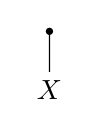
\begin{tikzpicture}[scale=0.75]
  \filldraw
    (0,0) node[fill=white] {$X$}
    --
    (0,1) circle (1.5pt) node[below right] {};
\end{tikzpicture}
\]
We want to be able to compose operations if one output matches an input of the other. For example, if we take
\begin{align*}
  f
  \in
  O(X_{1},X_{2},X_{3},X)
  \\
  f_{1}
  \in
  O(X_{11},X_{12},X_{1})
  \\
  f_{2}
  \in
  O(\emptyset,X)
  \\
  f_{3}
  \in
  O(X_{31},X_{3})
\end{align*}
then we want the composition illustrated by
\[
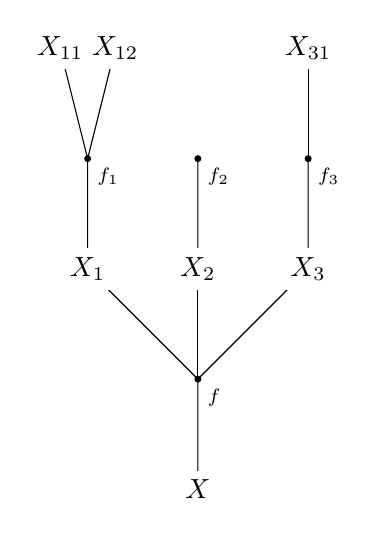
\begin{tikzpicture}[scale=0.70]
  \filldraw
    (0,0) node[fill=white] {$X$}
    --
    (0,2) circle (1.5pt) node[below right] {\scriptsize{$f$}};
  \draw
    (0,2)
    --
    (-2,4) node[fill=white] {$X_{1}$};
  \draw
    (0,2)
    --
    (0,4) node[fill=white] {$X_{2}$};
  \draw
    (0,2)
    --
    (2,4) node[fill=white] {$X_{3}$};
  \filldraw
    (-2,4) node[fill=white] {$X_{1}$}
    --
    (-2,6)
    circle (1.5pt) node[below right] {\scriptsize{$f_{1}$}};
  \draw
    (-2,6)
    --
    (-2.5,8) node[fill=white] {$X_{11}$};
  \draw
    (-2,6)
    --
    (-1.5,8) node[fill=white] {$X_{12}$};
  \filldraw
    (0,4) node[fill=white] {$X_{2}$}
    --
    (0,6) circle (1.5pt) node[below right] {\scriptsize{$f_{2}$}};
  \filldraw
    (2,4) node[fill=white] {$X_{3}$}
    --
    (2,6) circle (1.5pt) node[below right] {\scriptsize{$f_{3}$}};
  \draw
    (2,6)
    --
    (2,8) node[fill=white] {$X_{31}$};
\end{tikzpicture}
\]
to exist such that this composition is associative and in each set $O(X_{1},X_{2})$ with $X_{1},X_{2}$ arbitrary there is an element for each arrow from $X_{1}$ to $X_{2}$ in $\mathbf{C}$ behaving like an identity for identity arrows under the operad composition. Moreover one demands the composition to be {\glqq}stable{\grqq} under permutations of the input. What all this means precisely has to be looked up in a source about operads such as \cite{0d7b89ad}. It shall be not very surprising that operads abstractly track composition and hence that they have applications in higher category theory. Indeed, they are the backbone of a serious attempt to define weak $n$-category by Baez and Dolan in \cite{0d7b89ad}. It is not used much any more due to the addressed problems of weak $n$-categories for finite $n$ but it is a landmark paper in higher category theory and provides much intuition about the idea of higher category theory (and also operads). However, you might wish to first read \cite{de09a3f9} followed by \cite{c2d89e8a} which escort you more or less softly into the realms of higher category theory. In general, all the Baez stuff is highly recommended.



\section{Simplicial Set}
\label{sec:sset}
%\nocite{b28b8d8f}
%\nocite{4dd1b85f}
%\nocite{a565d200}
%\nocite{c82f5e22}
%\nocite{4dc38f27}
%\nocite{d09756a3}
%\nocite{6d9ad807}
%\nocite{00000011}
%TODO
%  formalize internal nerve
Simplicial sets model homotopy types as well as topological spaces do. This can be made formal using an equivalence on a $(\infty,1)$-topos level or more commonly (but essentially equivalent) a \textit{Quillen equivalence} on the \textit{model category}\footnote{we will briefly allude to them in the next section \ref{sec:fibration}} level. However, we will not really discuss this in this generality in this section. This was just the attention-getter. Yet, it should become clear on a more intuitive level that it works. For we will explain how one can build a CW complex from a simplicial set which will be a certain presheaf consisting of {\glqq}triangles of any dimension{\grqq}. One calls this geometric realization of the simplicial set. Before we do this we provide motivation for simplicial sets - combinatorial and geometrical - and compare a bit to the traditional notion of the quite rigid \textit{simplicial complexes}. We then geometrically motivate how we can utilize the machinery developed in subsubsection \ref{sec:coyoneda2} to geometrically realize with the Kan extenstions of the Yoneda functor. The same machinery applies for truncation of higher homotopy information as we will see when it comes to the nerve functor. This naturally leads to thoughts about the classification of principal bundles in $\mathbf{Top}$ by certain homotopy classes and then \v{C}ech cohomology which then in turn classify these homotopy classes. We conclude the section with a sequel of the generalized spaces example.
\\\\
To start off with, if you know some algebraic topology you might know simplicial complexes which are special cases of simplicial sets in that we allow for degenerate simplices in all dimensions in simplicial sets. This means that e.g. a point or a line can be considered a triangle. This is what makes simplicial sets way more flexible (just like a CW complex) than the rigid simplicial complexes. However, if you do not know simplicial complexes this does not help you much and we try to start from scratch. First we have to settle the question what a simplex of some dimension means. Well an $N$-simplex for $N \in \mathbb{N}$ shall be an $N$-dimensional version of a triangle. Geometrically, for $N \in \mathbb{N}$ the set
\begin{align*}
  \blacktriangle^{[N]}
  &:=
  \left\lbrace
      (x_{1},x_{2},\ldots,x_{N+1})
      \in
      \mathbb{R}^{N+1}
    \,
    \vert
    \,
      x_{i}
      \in
      [0,1]
      \,
      \land
      \,
      \sum_{i=1}^{N+1}
      x_{i}
      =
      1
  \right\rbrace
\end{align*}
topologized by the $\mathbb{R}^{N+1}$ subspace topology is called \textbf{$N$(-dimensional topological standard) simplex} which is just expressed by $N$-simplex. Let us illustrate the case $N = 0,1,2$ by
\[
\begin{tikzpicture}[scale=0.75]
  \fill[fill=green]
    (2,0) node[below] {$1$}
    circle
    (2pt);
  \draw[->]
    (0,0)
    --
    (4,0) node[right] {$x_{1}$};
\end{tikzpicture}
\]
\[
\begin{tikzpicture}[scale=0.75]
  \fill
    (2,0) node[below] {$1$}
    --
    (0,2) node[left] {$1$};
  \draw[green]
    (2,0)
    --
    (0,2);
  \draw[->]
    (0,0)
    --
    (4,0) node[right] {$x_{1}$};
  \draw[->]
    (0,0)
    --
    (0,4) node[above] {$x_{2}$};
\end{tikzpicture}
\]
\[
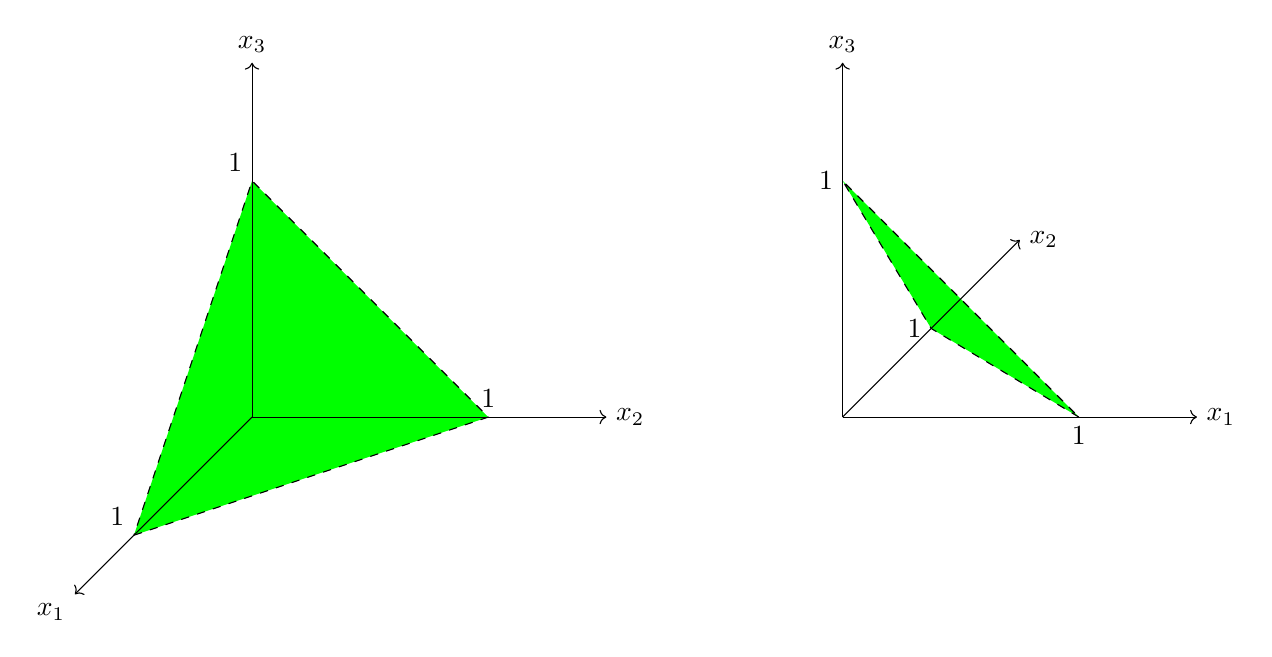
\begin{tikzpicture}[scale=0.75]
  \filldraw[dashed,fill=green]
    (-7,-2) node[above left] {$1$}
    --
    (-1,0) node[above] {$1$}
    --
    (-5,4) node[above left] {$1$}
    --
    cycle;
  \draw[->]
    (-5,0)
    --
    (-8,-3) node[below left] {$x_{1}$};
  \draw[->]
    (-5,0)
    --
    (1,0) node[right] {$x_{2}$};
  \draw[->]
    (-5,0)
    --
    (-5,6) node[above] {$x_{3}$};
  \filldraw[dashed,fill=green]
    (9,0) node[below] {$1$}
    --
    (6.5,1.5) node[left] {$1$}
    --
    (5,4) node[left] {$1$}
    --
    cycle;
  \draw[->]
    (5,0)
    --
    (11,0) node[right] {$x_{1}$};
  \draw[->]
    (5,0)
    --
    (8,3) node[right] {$x_{2}$};
  \draw[->]
    (5,0)
    --
    (5,6) node[above] {$x_{3}$};
\end{tikzpicture}
\]
$\blacktriangle^{[2]}$ is the triangle bounded by the dashed lines. Unfortunately, we cannot draw higher dimensions this way but $N = 3$ would be pyramid-shaped which can at least be illustrated as
\[
\begin{tikzpicture}[scale=0.75]
  \draw
    (-2,-2) 
    --
    (4,0)
    --
    (0,4)
    --
    cycle;
  \draw
    (0,0)
    --
    (-2,-2);
  \draw
    (0,0)
    --
    (4,0);
  \draw
    (0,0)
    --
    (0,4);
\end{tikzpicture}
\]
Now how can we capture this geometric information combinatorially? Actually, it suffices to know the dimension of the standard simplex we want to draw. So combinatorially we can consider the $N$-dimensional standard simplex as the set
\begin{align*}
  [N]
  &:=
  \lbrace
      n
      \in
      \mathbb{N}^{\times}
    \,
    \vert
    \,
      n
      \leq
      N
      +
      1
  \rbrace
\end{align*}
for all $N \in \mathbb{N}$ where we can consider the elements of $[N]$ as the corners of the $N$-simplex. In this way we have a natural order of the corners which is reflected as induced well-order on $[N]$ by the well-order of the natural number. Let us denote this
\begin{align*}
  [N]
  \doteq
  ([N],\leq)
  &\doteq
  ([N],\leq_{[N]})
\end{align*}
where $\leq_{[N]}$ is the restriction of the standard well-order $\leq_{\mathbb{N}}$ on the natural numbers. But $\blacktriangle^{[N]}$ contains even more information. Namely all the standard simplices of dimension lower than $N$ which can be embedded in the $N$-dimensional topological simplex in an order-preserving way. That is, we can restrict the $N$-dimensional topological simplex to get those of lower dimension. For example we have three possibilities of embedding the $1$-dimensional topological simplex into the $2$-dimensional topological simplex in an order-preserving way indicated by the following picture
\[
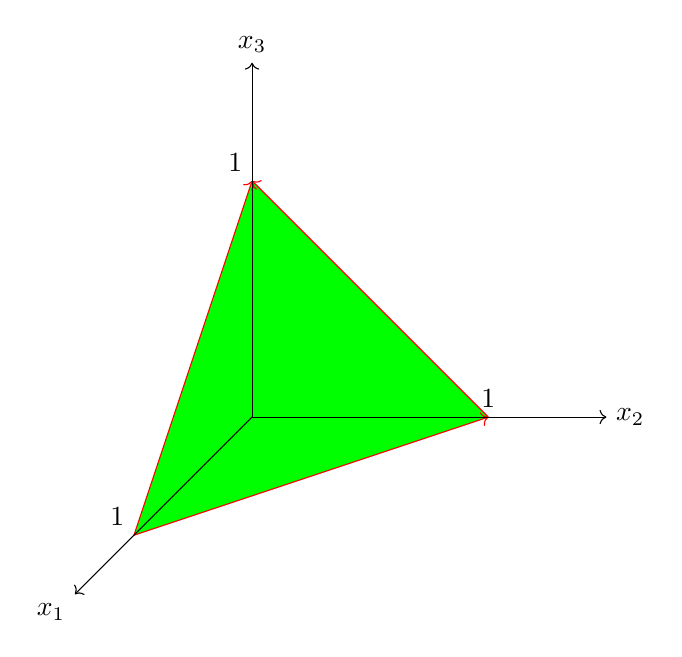
\begin{tikzpicture}[scale=0.75]
  \fill[fill=green]
    (-2,-2) node[above left] {$1$}
    --
    (4,0) node[above] {$1$}
    --
    (0,4) node[above left] {$1$}
    --
    cycle;
  \draw[->,red]
    (-2,-2)
    --
    (4,0);
  \draw[->,red]
    (-2,-2)
    --
    (0,4);
  \draw[->,red]
    (4,0)
    --
    (0,4);
  \draw[->]
    (0,0)
    --
    (-3,-3) node[below left] {$x_{1}$};
  \draw[->]
    (0,0)
    --
    (6,0) node[right] {$x_{2}$};
  \draw[->]
    (0,0)
    --
    (0,6) node[above] {$x_{3}$};
\end{tikzpicture}
\]
where the arrows symbolize the order of the embedded $1$-dimensional topological simplex. Combinatorially, we get for $i \in [N]$ functions
\begin{align*}
  \delta_{N,i}
  \colon
  [N-1]
  &\rightarrow
  [N]
  \\
  n
  &\mapsto
  \begin{cases}
    n
    &
    \text{for }
    n
    <
    i
    \\
    n
    +
    1
    &
    \text{for }
    n
    \geq
    i
  \end{cases}
\end{align*}
$\delta_{N,i}$ are precisely the strictly\footnote{with $<$ instead of $\leq$ in the order-preserving definition} order-preserving functions from $[N-1]$ to $[N]$. Even better: for all $N > 0$ the strictly order-preserving functions from $[N-k]$ to $[N]$ with $1 \leq k \leq N$ always decompose (not uniquely in general) as
\begin{align*}
  \delta_{N,i_{N}}
  \circ
  \cdots
  \circ
  \delta_{N-k+1,i_{N-k+1}}
\end{align*}
for some combination $(i_{N-k+1},\ldots,i_{N})$. But this shall not concern us here much. More important is the observation that restricting the object set of the category of well-ordered sets $\mathbf{WO}$ (see subsection \ref{sec:cat}) to only the well-ordered sets of the sort $([N],\leq)$ for some $N$ yields a full subcategory $\mathbf{\Delta}$. We call $\mathbf{\Delta}$ the \textbf{simplex category}.\footnote{note that $([N],\leq)$ corresponds itself to a category - the poset-category (again see subsection \ref{sec:cat}) - but this will only be important in construction \ref{cst:nerve} below} You might object that according to the above we should restrict $\mathbf{\Delta}$ to the subcategory $\mathbf{\Delta}_{\neq}$ with only \underline{strictly} order-preseving functions. For the record: let us call $\mathbf{\Delta}_{\neq}$ the \textbf{strict simplex category}. One can do that and in some cases it might be reasonable but usually it is an artifical restriction yielding a too rigid construction to be feasible in many applications. This is because if we take any order-preserving function into account then we in particular have order-preserving functions
\begin{align*}
  \sigma_{N,i}
  \colon
  [N + 1]
  &\rightarrow
  [N]
  \\
  n
  &\mapsto
  \begin{cases}
    n
    &
    \text{for }
    n
    \leq
    i
    \\
    n
    -
    1
    &
    \text{for }
    n
    >
    i
  \end{cases}
\end{align*}
for $i \in [N]$. And if the $\delta_{N,i}$ tell how we can restrict to lower dimension then the $\sigma_{N,i}$ must tell how we can consider $N$-dimensions as {\glqq}degenerated{\grqq} $N+1$-dimensions. This is to say that e.g. a point or a line are a degenerated triangle. This is the point where the flexibility of the soon defined simplicial sets originates from. Furthermore note that one can show that a morphism in $\mathbf{\Delta}$ decomposes as a combination of all $\delta_{N_{1},i}$ and all $\sigma_{N_{2},i}$ for $N_{1},N_{2} \in \mathbb{N}$ in an analogous manner as above where all non-identity morphisms in $\mathbf{\Delta}_{\neq}$ decomposed as a combination of $\delta_{N,i}$. But also this fact shall not concern us much here. After all we can define functors
\begin{align*}
  \vert
    \cdot
  \vert^{\textrm{stand}}
  \colon
  \mathbf{\Delta}
  &\rightarrow
  \mathbf{Top}
  \\
  [N]
  &\mapsto
  \blacktriangle^{[N]}
  \\
  \left(
    f
    \colon
    [N_{1}]
    \rightarrow
    [N_{2}]
  \right)
  &\mapsto
  \left(
    \sum_{i=1}^{N_{1}+1}
    x_{i}e_{i}
    \mapsto
    \sum_{i=1}^{N_{1}+1}
    x_{i}e_{f(i)}
  \right)
  \\\\
  \vert
    \cdot
  \vert_{\neq}^{\textrm{stand}}
  \colon
  \mathbf{\Delta}_{\neq}
  &\rightarrow
  \mathbf{Top}
  \\
  [N]
  &\mapsto
  \blacktriangle^{[N]}
  \\
  \left(
    f
    \colon
    [N_{1}]
    \rightarrow
    [N_{2}]
  \right)
  &\mapsto
  \left(
    \sum_{i=1}^{N_{1}+1}
    x_{i}e_{i}
    \mapsto
    \sum_{i=1}^{N_{1}+1}
    x_{i}e_{f(i)}
  \right)
\end{align*}
where $e_{i}$ denotes the $i$-th canonical basis vector of $\mathbb{R}^{n}$. We call $\vert \cdot \vert^{\textrm{stand}}$ the \textbf{geometric realization (of the standard simplices)} while $\vert \cdot \vert_{\neq}^{\textrm{stand}}$ is called the \textbf{geometric realization (of the strict standard simplices)}.
\\\\
Now what is the purpose of simplices? Well, in classical homotopy theory one usually tries to divide a space into simpler pieces which one knows very well from a homotopy perspective in a manner preserving the homotopy structure. The usual way to do this are CW complexes which model a space by balls of any dimension (this always works up to coherent homotopy). But in classical homotopy theory with topological spaces there is no combinatorial counterpart.\footnote{in UFP-HoTT the distinction becomes a bit more blurry (which is good in this case)} Therefore one used to take so-called simplicial complexes in the early days of algebraic topology. Loosely speaking, one divides a space into simplices of any dimension that allows for a combinatorial treatment. However, one needs many simplices to divide up comparably simple spaces such as a torus, for example: note that a (topological) torus is often defined as the space $[0,1] \times [0,1]$ modulo the equivalence relation generated by
\begin{align*}
  (0,t)
  &\sim
  (1,t)
  \\
  (t,0)
  &\sim
  (t,1)
\end{align*}
This is illustrated by
\[
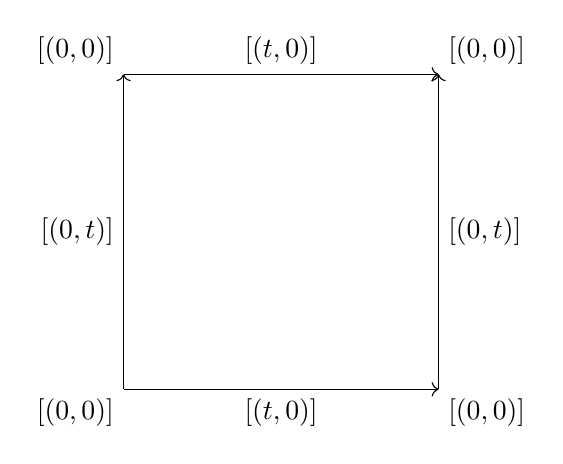
\begin{tikzpicture}[scale=4]
  \draw[->]
    (0,0) node[below left] {$[(0,0)]$}
    -- node[below] {$[(t,0)]$}
    (1,0) node[below right] {$[(0,0)]$};
  \draw[->]
    (0,1) node[above left] {$[(0,0)]$}
    -- node[above] {$[(t,0)]$}
    (1,1) node[above right] {$[(0,0)]$};
  \draw[->]
    (0,0)
    -- node[left] {$[(0,t)]$}
    (0,1) ;
  \draw[->]
    (1,0)
    -- node[right] {$[(0,t)]$}
    (1,1);
\end{tikzpicture}
\]
and we would like to divide the torus up in
\begin{enumerate}
\item[$\bullet$]
$2$ triangles $\triangle_{1}$ and $\triangle_{2}$
\item[$\bullet$]
$3$ lines $\upharpoonleft$, $\rightharpoonup$ and $\nearrow$
\item[$\bullet$]
$1$ corner $\centerdot$
\end{enumerate}
as illustrated by
\[
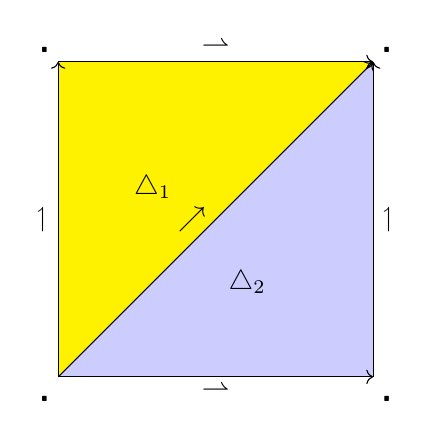
\begin{tikzpicture}[scale=4]
  \fill[yellow]
    (0,0)
    --
    (0,1)
    --
    (1,1)
    --
    cycle;
  \fill[blue!20]
    (0,0)
    --
    (1,0)
    --
    (1,1)
    --
    cycle;
  \draw
    (0.3,0.6) node {$\triangle_{1}$};
  \draw
    (0.6,0.3) node {$\triangle_{2}$};
  \draw[->]
    (0,0) node[below left] {$\centerdot$}
    -- node[below] {$\rightharpoonup$}
    (1,0) node[below right] {$\centerdot$};
  \draw[->]
    (0,1) node[above left] {$\centerdot$}
    -- node[above] {$\rightharpoonup$}
    (1,1) node[above right] {$\centerdot$};
  \draw[->]
    (0,0)
    -- node[left] {$\nearrow$}
    (1,1);
  \draw[->]
    (0,0)
    -- node[left] {$\upharpoonleft$}
    (0,1);
  \draw[->]
    (1,0)
    -- node[right] {$\upharpoonleft$}
    (1,1);
\end{tikzpicture}
\]
We do not want to expilcitly say here what a simplicial complex is but this is not a simplicial complex since $\triangle_{1}$ has the same faces as $\triangle_{2}$ and for a simplicial complex structure on the torus one would at least need $14$ triangles. What we rather have here are three sets
\begin{align*}
  &
  \lbrace
    \triangle_{1},
    \triangle_{2}
  \rbrace
  \\
  &
  \lbrace
    \upharpoonleft,
    \rightharpoonup,
    \nearrow
  \rbrace
  \\
  &
  \lbrace
    \centerdot
  \rbrace
\end{align*}
and
\begin{align*}
  \rightharpoonup
  &\text{ is the first face of }
  \triangle_{1}
  \\
  \nearrow
  &\text{ is the second face of }
  \triangle_{1}
  \\
  \upharpoonleft
  &\text{ is the third face of }
  \triangle_{1}
  \\
  \upharpoonleft
  &\text{ is the first face of }
  \triangle_{2}
  \\
  \nearrow
  &\text{ is the second face of }
  \triangle_{2}
  \\
  \rightharpoonup
  &\text{ is the third face of }
  \triangle_{2}
\end{align*}
Hence we can try to define a functor $\odot \colon \mathbf{\Delta}_{\neq}^{\mathrm{op}} \rightarrow \mathbf{Set}$ with
\begin{align*}
  \odot([0])
  &:=
  \lbrace
    \centerdot
  \rbrace
  \\
  \odot([1])
  &:=
  \lbrace
    \upharpoonleft,
    \rightharpoonup,
    \nearrow
  \rbrace
  \\
  \odot([2])
  &:=
  \lbrace
    \triangle_{1},
    \triangle_{2}
  \rbrace
  \\
  \odot(\delta_{2,1})
  &:=
  \lbrace
    (\triangle_{1},\rightharpoonup),
    (\triangle_{2},\upharpoonleft)
  \rbrace
  \\
  \odot(\delta_{2,2})
  &:=
  \lbrace
    (\triangle_{1},\nearrow),
    (\triangle_{2},\nearrow)
  \rbrace
  \\
  \odot(\delta_{2,3})
  &:=
  \lbrace
    (\triangle_{1},\upharpoonleft),
    (\triangle_{2},\rightharpoonup)
  \rbrace
  \\
  \odot(\delta_{1,i})
  &:=
  \lbrace
    (\rightharpoonup,\centerdot),
    (\nearrow,\centerdot),
    (\upharpoonleft,\centerdot)
  \rbrace
\end{align*}
and the obvious on the identity arrows of $\mathbf{\Delta}_{\neq}^{\mathrm{op}}$. Further we require $\odot$ to be on the composition of the various fitting $\delta_{N,i}$ such that $\odot$ respects composition and $F([N]) = \emptyset$ for $N > 2$. Then $\odot$ is apparently a functor by construction and captures the combinatorial data we imposed on the torus.
\\\\
This torus example suggests some terminology: a functor $F \colon \mathbf{\Delta}_{\neq}^{\mathrm{op}} \rightarrow \mathbf{Set}$ is called \textbf{strict simplicial set}. And we immediately generalize (as is proper for a real category theorist) to: a functor $F \colon \mathbf{\Delta}^{\mathrm{op}} \rightarrow \mathbf{Set}$ is called \textbf{simplicial set}. Note that the {\glqq}strict{\grqq} terminology is presumably not very common since we made it up. More common is semi-simplicial set or delta sets for strict simplicial sets. Altogether the terminology is historically a bit confusing and further discussed in \cite{8b5861fc} and \cite{4dd1b85f}. Both sources provide alternative intuition on the subject of strict simplicial sets and semi-simplicial sets we do not mention here. Other worthwhile sources are \cite{d09756a3} and a little more advanced \cite{b28b8d8f}. Anyways, both simplicial sets and its strict special case give rise to catgeories as functor categories
\begin{align*}
  \mathbf{sSet}_{\neq}
  &:=
  \mathbf{Set}^{\mathbf{\Delta}_{\neq}^{\mathrm{op}}}
  \\
  \mathbf{sSet}
  &:=
  \mathbf{Set}^{\mathbf{\Delta}^{\mathrm{op}}}
\end{align*}
where we call
\begin{enumerate}
\item[(1)]
$\mathbf{sSet}_{\neq}$ the \textbf{category of strict simplicial sets}
\item[(2)]
$\mathbf{sSet}$ the \textbf{category of simplicial sets}
\end{enumerate}
But this suggests what a strict simplicial map and a simplicial map shall be: natural transformations in the according category.
\begin{enumerate}
\item[(1)]
$\mathsf{S} \in \mathrm{Mor}_{\mathbf{sSet}_{\neq}}$ is called \textbf{strict simplicial map (from $\mathrm{dom}(\mathsf{S})$ to $\mathrm{cod}(\mathsf{S})$)}. For $\mathsf{S}$ being natural means that we have a family of functions
\begin{align*}
  \mathsf{S}([N])
  \colon
  \mathrm{dom}(\mathsf{S})([N])
  &\rightarrow
  \mathrm{cod}(\mathsf{S})([N])
\end{align*}
indexed by $N$. And since $\mathrm{dom}(\mathsf{S})([N])$ and $\mathrm{cod}(\mathsf{S})([N])$ are thought of as sets of $N$-simplices a strict simplicial map can be thought of as mapping simplices of a certain dimension to simplices of the same dimension. This is the same as it is for simplicial complexes. And this is where the rigid behaviour of simplicial complexes and hence strict simplicial sets comes from.
\item[(2)]
$\mathsf{S} \in \mathrm{Mor}_{\mathbf{sSet}}$ is called \textbf{simplicial map (from $\mathrm{dom}(\mathsf{S})$ to $\mathrm{cod}(\mathsf{S})$)}. For $\mathsf{S}$ being natural means that we have a family of functions
\begin{align*}
  \mathsf{S}([N])
  \colon
  \mathrm{dom}(\mathsf{S})([N])
  &\rightarrow
  \mathrm{cod}(\mathsf{S})([N])
\end{align*}
indexed by $N$. But $\mathrm{dom}(\mathsf{S})([N])$ and $\mathrm{cod}(\mathsf{S})([N])$ can now also contain degenerate $N$-simplices, that is, simplices of lower dimension than $N$ unlike in the strict case. This is to say that a simplicial map can be thought of as mapping $N$-simplices to simplices of equal or lower dimension than $N$. This is comparable to the situation of cellular maps for CW complexes which also map to lower or equal dimension. This is where the flexibility of CW complexes and hence simplicial sets comes from.\footnote{if you have worked through proofs of space approximation by simplicial complexes and CW complexes you might have recognized the convenience of CW complexes (see \cite{8b5861fc} for some possible proofs)}
\end{enumerate}
The next point is that strict simplicial sets and simplicial sets are some presheaeves on $\mathbf{\Delta}_{\neq}$ and $\mathbf{\Delta}$, respectively. According to our interpretation of presheaves in section \ref{sec:uni} we can consider them a generalized form of strict simplices and simplices, respectively, since we consider the objects of $\mathbf{\Delta}_{\neq}$ and $\mathbf{\Delta}$, respectively, as standard $N$-simplices. The standard simplices themselves can then be considered as strict simplicial sets and simplicial sets, respectively, by embedding them into presheaves by the Yoneda functor. Hence
\begin{enumerate}
\item[(1)]
the strict simplicial set
\begin{align*}
  \Delta_{\neq}^{N}
  &:=
  \mathrm{y}_{\mathbf{\Delta}_{\neq}}([N])
  =
  \mathrm{hom}_{\mathbf{\Delta}_{\neq}}(\cdot,[N])
\end{align*}
is called the \textbf{$N$(-dimensional strict categorical standard) simplex}
\item[(2)]
the simplicial set
\begin{align*}
  \Delta^{N}
  &:=
  \mathrm{y}_{\mathbf{\Delta}}([N])
  =
  \mathrm{hom}_{\mathbf{\Delta}}(\cdot,[N])
\end{align*}
is called the \textbf{$N$(-dimensional categorical standard) simplex}
\end{enumerate}
There is even more deserving an own name. $F(\delta_{2,1})$ for example maps a triangle to its first face. Thus if we are given a strict simplicial set $F \in \mathrm{ob}_{\mathbf{sSet}_{\neq}}$ define
\begin{align*}
  d_{N,i}^{F}
  &:=
  F(\delta_{N,i})
  \in
  \mathrm{mor}_{\mathbf{Set}}(F([N]),F([N-1]))
\end{align*}  
Then $d_{N,i}^{F}$ is called \textbf{$i$-th face map (of the $N$ simplices in $F$)}. This translates to simplicial sets essentially word for word: given a simplicial set $F \in \mathrm{ob}_{\mathbf{sSet}}$ define
\begin{align*}
  d_{N,i}^{F}
  &:=
  F(\delta_{N,i})
  \in
  \mathrm{mor}_{\mathbf{Set}}(F([N]),F([N-1]))
\end{align*}  
Then $d_{N,i}^{F}$ is called \textbf{$i$-th face map (of the $N$ simplices in $F$)}. But don't forget the $\sigma_{N,i}$ in this case which we interpreted as some way of allowing degeneracy. Hence given a simplicial set $F \in \mathrm{ob}_{\mathbf{sSet}}$ define
\begin{align*}
  s_{N,i}^{F}
  &:=
  F(\sigma_{N,i})
  \in
  \mathrm{mor}_{\mathbf{Set}}(F([N]),F([N+1]))
\end{align*}
Then $s_{N,i}^{F}$ is called \textbf{$i$-th degeneracy map (of the $N$ simplices in $F$)}.
\\\\
After this terminological excursion let us come back to our strict simplicial set $\odot$ containing the combinatorial data about our torus triangulation\footnote{dividing up into triangles}. Geometrically, we know how $\triangle_{1}$ and $\triangle_{2}$ are glued together. Can we reconstruct this from our combinatorial data (given by $\odot$) alone? For if so then it suffices to have $\odot$ and we could hope that the method works in general. This is to say we can geometrically realize any strict simplicial set and perhaps even simplicial set, making simplicial sets an improved version of CW complex if the geometric realization has a CW structure\footnote{spoiler: it has} due to its combinatorial aspect. Now what we definitely need for a geometric realization is an $N$-dimensional topological simplex for each element $\odot([N])$. This is to say we have a coproduct
\begin{align*}
  \coprod_{N=0}^{\infty}
  \odot([N])
  \times
  \blacktriangle^{[N]}
\end{align*}
where $\odot([N])$ shall have its power set as topology. Now we have to quotient out some things:
\begin{align*}
  \left(
    \triangle_{i},
    (0,x_{2},x_{3})
  \right)
  &\sim
  \left(
    d_{2,1}^{\odot}(\triangle_{i}),
    (x_{2},x_{3})
  \right)
  \\
  \left(
    \triangle_{i},
    (x_{1},0,x_{3})
  \right)
  &\sim
  \left(
    d_{2,2}^{\odot}(\triangle_{i}),
    (x_{1},x_{3})
  \right)
  \\
  \left(
    \triangle_{i},
    (x_{1},x_{2},0)
  \right)
  &\sim
  \left(
    d_{2,3}^{\odot}(\triangle_{i}),
    (x_{1},x_{2})
  \right)
  \\
  \left(
    \upharpoonleft,
    (0,x_{2})
  \right)
  &\sim
  \left(
    d_{1,1}^{\odot}(\upharpoonleft),
    x_{2}
  \right)
  \\
  \left(
    \upharpoonleft,
    (x_{1},0)
  \right)
  &\sim
  \left(
    d_{1,2}^{\odot}(\upharpoonleft),
    x_{1}
  \right)
  \\
  \left(
    \rightharpoonup,
    (0,x_{2})
  \right)
  &\sim
  \left(
    d_{1,1}^{\odot}(\rightharpoonup),
    x_{2}
  \right)
  \\
  \left(
    \rightharpoonup,
    (x_{1},0)
  \right)
  &\sim
  \left(
    d_{1,2}^{\odot}(\rightharpoonup),
    x_{1}
  \right)
  \\
  \left(
    \nearrow,
    (0,x_{2})
  \right)
  &\sim
  \left(
    d_{1,1}^{\odot}(\nearrow),
    x_{2}
  \right)
  \\
  \left(
    \nearrow,
    (x_{1},0)
  \right)
  &\sim
  \left(
    d_{1,2}^{\odot}(\nearrow),
    x_{1}
  \right)
\end{align*}
Let $\sim$ be the equivalence relation generated by these identifications. Then the quotient space
\begin{align*}
  \left.
    \left(
      \coprod_{N=0}^{\infty}
      \odot([N])
      \times
      \blacktriangle^{[N]}
    \right)
  \right\slash
  \sim
\end{align*}
can be shown to be strongly homotopy equivalent to the torus as should be intuitively clear from what we have done. This can be considered a certain coequalizer (it's not hard to find it but a bit tedious). Furthermore by observing that $\odot([N])$ in the coproduct above is for indexing purposes only it is quite obvious that
\begin{align*}
  \coprod_{N=0}^{\infty}
  \odot([N])
  \times
  \blacktriangle^{[N]}
  &\cong
  \coprod_{([N],x) \in \mathrm{ob}_{\int_{\mathbf{\Delta}_{\neq}}^{\prime}\odot}}
  \left\vert
    \pi_{\odot}([N],x)
  \right\vert_{\neq}^{\textrm{stand}}
\end{align*}
Hence we get\footnote{to see all this please note theorem \ref{thm:limitexistence}}
\begin{align*}
  \left.
    \left(
      \coprod_{N=0}^{\infty}
      \odot([N])
      \times
      \blacktriangle^{[N]}
    \right)
  \right\slash
  \sim
  &\cong
  \varinjlim_{\int_{\mathbf{\Delta}_{\neq}}^{\prime}\odot}
  \left(
    \vert
      \cdot
    \vert_{\neq}^{\textrm{stand}}
    \circ
    \pi_{\odot}
  \right)
\end{align*}
Now we recall subsubsection \ref{sec:coyoneda2} where we intensively discussed the density theorem \ref{cor:density} (the second version) and found that
\begin{align*}
  L_{\vert \cdot \vert_{\neq}^{\textrm{stand}}}
\end{align*}
such that
\begin{align*}
  L_{\vert \cdot \vert_{\neq}^{\textrm{stand}}}
  (\odot)
  &=
  \varinjlim_{\int_{\mathbf{\Delta}_{\neq}}^{\prime}\odot}
  \left(
    \vert
      \cdot
    \vert_{\neq}^{\textrm{stand}}
    \circ
    \pi_{\odot}
  \right)
\end{align*}
as a special case of construction \ref{cst:la} since $\mathbf{Top}$ is cocomplete by theorem \ref{thm:topcocomplete}. More concisely,
\begin{align*}
  L_{\vert \cdot \vert_{\neq}^{\textrm{stand}}}
\end{align*}
is the left Kan extension of $\vert \cdot \vert_{\neq}^{\textrm{stand}}$ along the yoneda functor $\mathrm{y}_{\mathbf{\Delta}_{\neq}}$. And this can be generalized to any strict simplicial set and even simplicial set allowing to geometrically realize any of both sorts. So define
\begin{align*}
  \vert
    \cdot
  \vert_{\neq}
  &:=
  \mathrm{Lan}_{\mathrm{y_{\mathbf{\Delta}_{\neq}}}}
  \vert
    \cdot
  \vert_{\neq}^{\textrm{stand}}
  \\
  \vert
    \cdot
  \vert
  &:=
  \mathrm{Lan}_{\mathrm{y_{\mathbf{\Delta}}}}
  \vert
    \cdot
  \vert^{\textrm{stand}}
\end{align*}
then the functor
\begin{enumerate}
\item[(1)]
$\vert \cdot \vert_{\neq}$ is called \textbf{geometric realization (of strict simplicial sets)}
\item[(2)]
$\vert \cdot \vert$ is called \textbf{geometric realization (of simplicial sets)}
\end{enumerate}
This definition makes sense since $\mathbf{Top}$ is cocomplete and since corollary \ref{cor:yonedauniarr} holds. In particular, we have
\begin{align*}
  \left\vert
    \Delta^{N}
  \right\vert
  &=
  \left\vert
    [N]
  \right\vert^{\textrm{stand}}
\end{align*}
expressing that $\vert \cdot \vert$ is an extension of $\vert \cdot \vert^{\textrm{stand}}$ by the interpretation that $\Delta^{N}$ is the presheaf version of the $N$-dimensional standard simplex. What we also want the reader to recognize is that $\vert \cdot \vert$ is functorial without any additional work. But it actually didn't just fall into our lap. We needed almost the whole one hundred pages of section \ref{sec:uni} to get it. In particular, it was comparably tricky for category theory circumstances to find out what $\vert \cdot \vert$ is on simplicial maps. Of course, we could have tried to find a proof of continuity of $\vert \mathsf{T} \vert$ for some simplicial map $\mathsf{T}$ directly using abstracted versions of the quotient space
\begin{align*}
  \left.
    \left(
      \coprod_{N=0}^{\infty}
      \odot([N])
      \times
      \blacktriangle^{[N]}
    \right)
  \right\slash
  \sim
\end{align*}
we used in the torus example. We do not know how easy that really is,\footnote{as far as we know Milnor claims somewhere that it is not too hard - but that doesn't mean a lot regarding ordinary mortals like the authors} but the method is inferior to ours in the sense that it does not apply more generally without any more efforts. Namely, instead of the simplex category $\mathbf{\Delta}$ we can take any other category with objects interpretable - that is, geometrically realizable in a functorial way in a cocomplete category as $\vert \cdot \vert^{\textrm{stand}}$ does with simplices of any dimension in $\mathbf{Top}$ - as $N$-dimensional versions of some geometric shape. Examples include globes and cubes. The former plays a role in some definitions of $n$-categories while the latter are somtimes used in homotopy theory, for example. But for the purpose of classical homotopy theory simplicial sets are superior to cubical sets for some reasons we do not want to list here (see e.g. \cite{wiki-nlab0000} article: cubical set - exposition). Another point is that we know that the left Kan extension of some functor along the Yoneda functor is left adjoint to the according functor from theorem \ref{thm:initprobisinitcone}. In particular, we get that $\vert \cdot \vert$ is left adjoint to the so-called singular set functor
\begin{align*}
  \mathrm{Sing}
  :=
  R_{\vert \cdot \vert^{\textrm{stand}}}
  \colon
  \mathbf{Top}
  &\rightarrow
  \mathbf{sSet}
  \\
  X
  &\mapsto
  \mathrm{hom}_{\mathbf{Top}}
  \left(
    \vert
      \cdot
    \vert^{\textrm{stand}},
    X
  \right)
  \\
  f_{12}
  &\mapsto
  \mathrm{hom}_{\mathbf{Top}}
  \left(
    \vert
      \cdot
    \vert^{\textrm{stand}},
    f_{12}
  \right)
\end{align*}
So $\mathrm{Sing}(Y)$ for some space $Y$ gives all the singular simplices where an $N$-dimensional singular simplex is an element of
\begin{align*}
  \mathrm{hom}_{\mathbf{Top}}
  \left(
    \left\vert
      [N]
    \right\vert^{\textrm{stand}},
    Y
  \right)
\end{align*}
The algebraic topologists among us thus might see a connection to singular homology. The following theorem completes our treatment of the geometric realization.
\\
\begin{thm}
\label{thm:ssetcwcompex}
\begin{enumerate}
\item[(1)]
For all $F \in \mathrm{ob}_{\mathbf{sSet}_{\neq}}$ the space $\vert F \vert_{\neq}$ is a CW complex.
\item[(2)]
For all $F \in \mathrm{ob}_{\mathbf{sSet}}$ the space $\vert F \vert$ is a CW complex.
\end{enumerate}
\end{thm}
\begin{prf}
See e.g. \cite{8b5861fc} for (1) and e.g. \cite{b28b8d8f} for (2).
\\
\phantom{proven}
\hfill
$\square$
\end{prf}
As a last remark if we restrict the codomain of the geometric realization of simplicial sets to a convenient category of spaces then the geometric realization preserves finite limits.\footnote{in topos language: if $\mathbf{sSet}$ and the convenient category of spaces are given a topoi structure the geometric realization together with the singular set functor is a so-called \textit{geometric morphism}}
\\\\
As we have seen, the geometric realization of simplicial sets is the left Kan extension of some functor from $\mathbf{\Delta}$ to $\mathbf{Top}$ along the yoneda functor $\mathrm{y}_{\mathbf{\Delta}}$.\footnote{this can be accordingly expressed in the strict case but we refrain from treating this case further in this section} But this construction works for any functor from $\mathbf{\Delta}$ to a cocomplete category. In particular, we have a right adjoint. All this we have found out in subsubsection \ref{sec:coyoneda2} and what we do now is considering a case of special interest when the cocomplete category is $\mathbf{Cat}$.\footnote{for the fact that $\mathbf{Cat}$ is bicomplete we have to refer to the literature such as \cite{52fbba46} which says a bit (but not much) about it}
\\
\begin{cst}[Nerve]
\label{cst:nerve}
Note that $([N],\leq)$ as well-ordered set can itself be considered as a category. Namely as the poset category $\pmb{\leq}_{[N]}$ of $([N],\leq)$. So we have a function from $\mathrm{ob}_{\mathbf{\Delta}}$ to $\mathrm{ob}_{\mathbf{Cat}}$ and it's natural to try making this the object part of a functor
\begin{align*}
  \vert
    \cdot
  \vert_{1}^{\textrm{stand}}
  \colon
  \mathbf{\Delta}
  &\rightarrow
  \mathbf{Cat}
\end{align*}
But an order-preserving function
\begin{align*}
  f
  &\in
  \mathrm{mor}_{\mathbf{\Delta}}
  \left(
    [N_{1}],
    [N_{2}]
  \right)
\end{align*}
precisely corresponds to the functor
\begin{align*}
  F_{f}
  \colon
  \pmb{\leq}_{[N_{1}]}
  &\rightarrow
  \pmb{\leq}_{[N_{2}]}
  \\
  n_{1}
  &\mapsto
  f(n_{1})
  \\
  (a,b)
  &\mapsto
  (f(a),f(b))
\end{align*}
where $F_{f}$ is well-defined, that is,
\begin{align*}
  (f(a),f(b))
  &\in
  \mathrm{Mor}_{\pmb{\leq}_{[N_{2}]}}
\end{align*}
if and only if $f$ is order-preserving. And hence we get a functor
\begin{align*}
  \vert
    \cdot
  \vert_{1}^{\textrm{stand}}
  \colon
  \mathbf{\Delta}
  &\rightarrow
  \mathbf{Cat}
  \\
  [N]
  &\mapsto
  \pmb{\leq}_{[N]}
  \\
  f
  &\mapsto
  F_{f}
\end{align*}
Let us call $\vert \cdot \vert_{1}^{\textrm{stand}}$ the \textbf{first standard truncation}. By applying theorem \ref{thm:initprobisinitcone} to $A = \vert \cdot \vert_{1}^{\textrm{stand}}$ we get a right adjoint functor
\begin{align*}
  \mathrm{n}
  :=
  R_{\vert \cdot \vert_{1}^{\textrm{stand}}}
  \colon
  \mathbf{Cat}
  &\rightarrow
  \mathbf{sSet}
  \\
  \mathbf{C}
  &\mapsto
  \mathrm{hom}_{\mathbf{Cat}}
  \left(
    \vert
      \cdot
    \vert_{1}^{\textrm{stand}},
    \mathbf{C}
  \right)
  \\
  F_{\alpha\beta}
  &\mapsto
  \mathrm{hom}_{\mathbf{Cat}}
  \left(
    \vert
      \cdot
    \vert_{1}^{\textrm{stand}},
    F_{\alpha\beta}
  \right)
\end{align*}
$\mathrm{n}$ is called the \textbf{nerve functor} and for $\mathbf{C} \in \mathrm{ob}_{\mathbf{Cat}}$ the functor
\begin{align*}
  \mathrm{n}(\mathbf{C})
  &=
  \mathrm{hom}_{\mathbf{Cat}}
  \left(
    \vert
      \cdot
    \vert_{1}^{\textrm{stand}},
    \mathbf{C}
  \right)
\end{align*}
is called \textbf{the nerve (of $\mathbf{C}$)}. The nerve functor $\mathrm{n}$ is fully faithful, that is, an embedding. This is to say that we can understand a category $\mathbf{C}$ by its nerve $\mathrm{n}(\mathbf{C})$. This can be seen to be sensible explicitly by examining what
\begin{align*}
  \mathrm{hom}_{\mathbf{Cat}}
  \left(
    \left\vert
      [N]
    \right\vert_{1}^{\textrm{stand}},
    \mathbf{C}
  \right)
\end{align*}
for some $N$ actually is. So we have to look at what a functor $F \colon \pmb{\leq}_{[N]} \rightarrow \mathbf{C}$ does. Well, since $\pmb{\leq}_{[N]}$ is a poset category, $F$ is nothing but a commuative diagram which can be graphically illustrated for $N$ small enough. Let us draw the cases $N = 0,1,2,3$ from which it should become clear what the general case may look like.
\[
\begin{tikzcd}[sep=large]
  F(1)
\end{tikzcd}
\]
\[
\begin{tikzcd}[sep=large]
  F(1)
  \arrow{r}{F(1,2)}
  &
  F(2)
\end{tikzcd}
\]
\[
\begin{tikzcd}[sep=large]
  &
  F(2)
  \arrow{rd}{F(2,3)}
  &
  \\
  F(1)
  \arrow{ru}{F(1,2)}
  \arrow{rr}{F(1,3)}
  &
  &
  F(3)
\end{tikzcd}
\]
\[
\begin{tikzcd}[sep=large]
  &
  F(2)
  \arrow{r}{F(2,3)}
  \arrow[swap,crossing over]{rrd}{F(2,4)}
  &
  F(3)
  \arrow{rd}{F(3,4)}
  &
  \\
  F(1)
  \arrow{ru}{F(1,2)}
  \arrow[swap,crossing over]{rru}{F(1,3)}
  \arrow{rrr}{F(1,4)}
  &
  &
  &
  F(4)
\end{tikzcd}
\]
So what $F \colon \pmb{\leq}_{[N]} \rightarrow \mathbf{C}$ actually does is choosing a list of arrows $F(1,2),\ldots,F(N,N+1)$ each composable with the preceding and succeding list entry. This is to say that $\mathrm{n}$ splits up the category $\mathbf{C}$ in any list of composable arrows and it is intuitively clear that the nerve of $\mathbf{C}$ contains all the information about this category since a category is nothing more than its arrows and how they can be composed. Hence it is clear that for $N \in \mathbb{N}$
\begin{align*}
  \mathrm{hom}_{\mathbf{Cat}}
  \left(
    \left\vert
      [N]
    \right\vert_{1}^{\textrm{stand}},
    \mathbf{C}
  \right)
  &\cong
  \prod_{\mathrm{ob}_{\mathbf{C}}}^{N}
  \mathrm{Mor}_{\mathbf{C}}
\end{align*}
where the latter denotes the $N$-fold fiber product of the domain function $\mathrm{dom}_{\mathbf{C}}$ and codomain function $\mathrm{cod}_{\mathbf{C}}$ in the case $N \geq 2$ and $\mathrm{Mor}_{\mathbf{C}}$ in the case $N = 1$ while being $\mathrm{ob}_{\mathbf{C}}$ in the case $N = 0$. This fiber product structure suggests a generalization by replacing $\mathbf{Set}$ with a category $\mathbf{C}$ with pullbacks. To this end first some terminology. For any category $\mathbf{C}$ (not necessarily with pullbacks at this point) a functor $F \colon \mathbf{\Delta}^{\mathrm{op}} \rightarrow \mathbf{C}$ is called \textbf{simplicial object (in $\mathbf{C}$)}. More specifically, a simplicial object in $\mathbf{Top}$ is called a \textbf{simplicial space}. Now if $\mathbf{C}$ has pullbacks and $\mathrm{Int}_{\mathbf{C}}$ is a category internal to $\mathbf{C}$ we call the simplicial object in $\mathbf{C}$ defined by\footnote{note that this is actually not directly well-defined since pullbacks are only up to isomorphism and we have to make a choice}
\begin{align*}
  \mathrm{n}_{\mathrm{Int}_{\mathbf{C}}}
  \doteq
  \mathrm{n}_{\mathrm{Int}_{\mathbf{C}}}^{\textrm{int}}
  \colon
  \mathbf{\Delta}^{\mathrm{op}}
  &\rightarrow
  \mathbf{C}
  \\
  [N]
  &\mapsto
  \prod_{\mathrm{ob}_{\mathrm{Int}_{\mathbf{C}}}}^{N}
  \mathrm{Mor}_{\mathrm{Int}_{\mathbf{C}}}
  \\
  f
  &\mapsto
  \mathrm{n}_{\mathrm{Int}_{\mathbf{C}}}(f)
\end{align*}
the\footnote{$\mathrm{n}_{\mathrm{Int}_{\mathbf{C}}^{\textrm{int}}}(f)$ can be derived by the interested reader from the $\mathbf{Set}$ case using the internal domain and codomain morphism} \textbf{(internal) nerve (of $\mathrm{Int}_{\mathbf{C}}$)} though strictly speaking we have not defined internal categories in these notes. However, for the purpose of these notes it suffices to have a feeling of what this internalization is - if at all. But now back to simplicial sets. From all we have seen we would even expect that only the cases $N = 0,1,2$ matter since for $N = 3$ and higher we can fall back to the case $N = 2$ as the last diagram suggests in the sense that the last diagram is a {\glqq}triangulation{\grqq} of the composition of $3$ arrows (the outer square) by $2$-simplices or better say triangles when considered in $3$ dimensions. This is due to the strict associativity or more precisely that we deal with strict $1$-categories. All in all we have the strong conjecture that
\begin{align*}
  \mathrm{hom}_{\mathbf{Cat}}
  \left(
    \left\vert
      [N]
    \right\vert_{1}^{\textrm{stand}},
    \mathbf{C}
  \right)
\end{align*}
consists of degenerated $2$-simplices. Further it can be conjectured that higher simplices play a role for the various compositions in weak higher categories if we are able to replace $\mathbf{Cat}$ by ${}_{(n,n)}\mathbf{Cat}$ and define an approriate notion of nerve. Indeed, simplicial sets are used much in higher category theory but all this is a subject for some other notes. Anyways, the first conjecture proves to be true in the sense that the left Kan extension
\begin{align*}
  \vert
    \cdot
  \vert_{1}
  &:=
  \mathrm{Lan}_{\mathrm{y}_{\mathbf{\Delta}}}
  \vert
    \cdot
  \vert_{1}^{\textrm{stand}}
\end{align*}
of $\vert \cdot \vert_{1}^{\textrm{stand}}$ along $\mathrm{y}_{\mathbf{\Delta}}$ is a left inverse/retraction (in the weak sense) to the nerve functor\footnote{this can be seen from the fact that $\mathrm{n}$ is an embedding right adjoint to $\vert \cdot \vert_{1}$ by lemma $4$ of section II.6 in \cite{c55c71e8} which is a more general version of our corollary \ref{cor:adjointequiv}} and $\vert \cdot \vert_{1}$ is determined by whereto it maps simplicial sets restricted to $[0],[1],[2]$ and the order-preserving functions between those. Note that $\vert \cdot \vert_{1}$ can be chosen to be the left adjoint to the nerve functor $\mathrm{n}$ from construction \ref{cst:la} as we saw in corollary \ref{cor:yonedauniarr}. Moreover $\vert \cdot \vert_{1}$ is called the \textbf{first truncation} and this terminology is not just a coincidence with the $1$-truncation defined in UFP-HoTT we briefly discussed in section \ref{sec:metaidea}. This has to do with the fact that simplicial sets can be used to model homotopy theory as one classically does with topological spaces, that is, one has paths in any dimension while categories have only paths in dimension $0$ and $1$. Further the discussion above makes intuitively clear a bit that $\vert \cdot \vert_{1}$ truncates what happens above level $1$ - at least we hope so.
\end{cst}
\begin{prf}
The correspondence of $f$ to $F_{f}$ and the functoriality of $F_{f}$ as well as this of $\vert \cdot \vert_{1}^{\textrm{stand}}$ is not hard to see and left to the reader. Also, we leave the proof that $\vert \cdot \vert_{1}^{\textrm{stand}}$ is faithful to the reader.
\\
What we prove is that $\mathrm{n}$ is fully faithful.
\begin{description}
\item[Step 1]
We first show that $\mathrm{n}$ is faithful: Take functors
\begin{align*}
  F,
  F^{\backprime}
  \in
  \mathrm{mor}_{\mathbf{Cat}}
  \left(
    \mathbf{C}_{\alpha},
    \mathbf{C}_{\beta}
  \right)
\end{align*}
and assume
\begin{align*}
  F
  &\neq
  F^{\backprime}
\end{align*}
Then we have the inequality
\begin{align*}
  (\mathrm{n}(F))
  \left(
    [1]
  \right)
  &=
  \mathrm{hom}_{\mathbf{Cat}}
  \left(
    \left\vert
      [1]
    \right\vert_{1}^{\textrm{stand}},
    F
  \right)
  \\
  &\neq
  \mathrm{hom}_{\mathbf{Cat}}
  \left(
    \left\vert
      [1]
    \right\vert_{1}^{\textrm{stand}},
    F^{\backprime}
  \right)
  \\
  &=
  \left(
    \mathrm{n}(F^{\backprime})
  \right)
  \left(
    [1]
  \right)
\end{align*}
since
\begin{align*}
  \mathrm{hom}_{\mathbf{Cat}}
  \left(
    \left\vert
      [1]
    \right\vert_{1}^{\textrm{stand}},
    F
  \right)
\end{align*}
is just composition with $F$ and likewise for $F^{\backprime}$ and
\begin{align*}
  \mathrm{hom}_{\mathbf{Cat}}
  \left(
    \left\vert
      [1]
    \right\vert_{1}^{\textrm{stand}},
    \mathbf{C}_{\alpha}
  \right)
\end{align*}
can be identified with $\mathrm{Mor}_{\mathbf{C}_{\alpha}}$. But different functors are different on the morphisms. Hence
\begin{align*}
  \mathrm{n}(F)
  &\neq
  \mathrm{n}
  \left(
    F^{\backprime}
  \right)
\end{align*}
showing that $\mathrm{n}$ is faithful.
\item[Step 2]
Now we show that $\mathrm{n}$ is also full: let
\begin{align*}
  \mathsf{S}
  \in
  \mathrm{mor}_{\mathbf{sSet}}
  \left(
    \mathrm{n}(\mathbf{C}_{\alpha}),
    \mathrm{n}(\mathbf{C}_{\beta})
  \right)
\end{align*}
This is to say functions
\begin{align*}
  \mathsf{S}([N])
  \colon
  \mathrm{hom}_{\mathbf{Cat}}
  \left(
    \left\vert
      [N]
    \right\vert_{1}^{\textrm{stand}},
    \mathbf{C}_{\alpha}
  \right)
  &\rightarrow
  \mathrm{hom}_{\mathbf{Cat}}
  \left(
    \vert
      [N]
    \vert_{1}^{\textrm{stand}},
    \mathbf{C}_{\beta}
  \right)
\end{align*}
such that for all $N_{1},N_{2} \in \mathbb{N}$ and all order-preserving functions $f \colon [N_{1}] \rightarrow [N_{2}]$
\[
\begin{tikzcd}[row sep=huge, column sep=15ex]
  \mathrm{hom}_{\mathbf{Cat}}
  \left(
    \pmb{\leq}_{[N_{2}]},
    \mathbf{C}_{\alpha}
  \right)
  \arrow{r}{\mathrm{hom}_{\mathbf{Cat}}(F_{f},\mathbf{C}_{\alpha})}
  \arrow[swap]{d}{\mathsf{S}([N_{2}])}
  &
  \mathrm{hom}_{\mathbf{Cat}}
  \left(
    \pmb{\leq}_{[N_{1}]},
    \mathbf{C}_{\alpha}
  \right)
  \arrow{d}{\mathsf{S}([N_{1}])}
  \\
  \mathrm{hom}_{\mathbf{Cat}}
  \left(
    \pmb{\leq}_{[N_{2}]},
    \mathbf{C}_{\beta}
  \right)
  \arrow{r}{\mathrm{hom}_{\mathbf{Cat}}(F_{f},\mathbf{C}_{\beta})}
  &
  \mathrm{hom}_{\mathbf{Cat}}
  \left(
    \pmb{\leq}_{[N_{1}]},
    \mathbf{C}_{\beta}
  \right)
\end{tikzcd}
\]
Now let for all $X^{\alpha}$
\begin{align*}
  I_{X^{\alpha}}
  &\in
  \mathrm{hom}_{\mathbf{Cat}}
  \left(
    \left\vert
      [0]
    \right\vert_{1}^{\textrm{stand}},
    \mathbf{C}_{\alpha}
  \right)
\end{align*}
be the unique element such that $I_{X^{\alpha}}(1) = X^{\alpha}$ and note that this gives a bijection
\begin{align*}
  \mathrm{ob}_{\mathbf{C}}
  &\cong
  \mathrm{hom}_{\mathbf{Cat}}
  \left(
    \left\vert
      [0]
    \right\vert_{1}^{\textrm{stand}},
    \mathbf{C}_{\alpha}
  \right)
\end{align*}
In very much the same way we define for $f_{12}^{\alpha}$
\begin{align*}
  I_{f_{12}^{\alpha}}
  &\in
  \mathrm{hom}_{\mathbf{Cat}}
  \left(
    \left\vert
      [1]
    \right\vert_{1}^{\textrm{stand}},
    \mathbf{C}_{\alpha}
  \right)
\end{align*}
as the unique element such that $I_{f_{12}^{\alpha}}((1,2)) = f_{12}^{\alpha}$ and note that this gives a bijection
\begin{align*}
  \mathrm{mor}_{\mathbf{C}}(X_{1}^{\alpha},X_{2}^{\alpha})
  &\cong
  \mathrm{hom}_{\mathbf{Cat}}
  \left(
    \left\vert
      [1]
    \right\vert_{1}^{\textrm{stand}},
    \mathbf{C}_{\alpha}
  \right)
\end{align*}
Then define the functor
\begin{align*}
  F_{\mathsf{S}}
  \colon
  \mathbf{C}_{\alpha}
  &\rightarrow
  \mathbf{C}_{\beta}
  \\
  X^{\alpha}
  &\mapsto
  \mathsf{S}([0])(I_{X^{\alpha}})(1)
  \\
  f_{12}^{\alpha}
  &\mapsto
  \mathsf{S}([1])(I_{f_{12}^{\alpha}})(1,2)
\end{align*}
Let us show that $F_{\mathsf{S}}$ is indeed a functor: for
\begin{align*}
  f
  &:=
  \left(
    [1],
    [0],
    \left\lbrace
      (1,1),
      (2,1)
    \right\rbrace
  \right)
\end{align*}
we get by naturality of $\mathsf{S}$
\begin{align*}
  F_{\mathsf{S}}
  \left(
    \mathrm{id}_{X^{\alpha}}
  \right)
  &=
  \mathsf{S}([1])
  \left(
    I_{\mathrm{id}_{X^{\alpha}}}
  \right)
  (1,2)
  \\
  &=
  \mathsf{S}([1])
  \left(
    I_{X^{\alpha}}
    \circ
    F_{f}
  \right)
  (1,2)
  \\
  &=
  \left(
    \mathsf{S}([0])
    \left(
      I_{X^{\alpha}}
    \right)
    \circ
    F_{f}
  \right)
  (1,2)
  \tag{NT}
  \\
  &=
  \mathsf{S}([0])
  \left(
    I_{X^{\alpha}}
  \right)
  (1,1)
  \\
  &=
  \mathrm{id}_{F_{\mathsf{S}}(X^{\alpha})}
\end{align*}
Moreover for
\begin{align*}
  f
  &:=
  \left(
    [1],
    [2],
    \left\lbrace
      (1,1),
      (2,3)
    \right\rbrace  
  \right)
  \\
  f_{1}
  &:=
  \left(
    [1],
    [2],
    \left\lbrace
      (1,1),
      (2,2)
    \right\rbrace
  \right)
  \\
  f_{2}
  &:=
  \left(
    [1],
    [2],
    \left\lbrace
      (1,2),
      (2,3)
    \right\rbrace
  \right)
\end{align*}
and $I_{f_{23}^{\alpha} \circ f_{12}^{\alpha}}^{2}$
\begin{align*}
  I_{f_{23}^{\alpha} \circ f_{12}^{\alpha}}^{2}
  &\in
  \mathrm{hom}_{\mathbf{Cat}}
  \left(
    \left\vert
      [2]
    \right\vert_{1}^{\textrm{stand}},
    \mathbf{C}_{\alpha}
  \right)
\end{align*}
the unique element such that
\begin{align*}
  I_{f_{23}^{\alpha} \circ f_{12}^{\alpha}}^{2}(2,3)
  &=
  I_{f_{23}^{\alpha}}(1,2)
  \\
  I_{f_{23}^{\alpha} \circ f_{12}^{\alpha}}^{2}(1,2)
  &=
  I_{f_{12}^{\alpha}}(1,2)
\end{align*}
we get by naturality of $\mathsf{S}$
\begin{align*}
  F_{\mathsf{S}}
  \left(
    f_{23}^{\alpha}
    \circ
    f_{12}^{\alpha}
  \right)
  &=
  \mathsf{S}([1])
  \left(
    I_{f_{23}^{\alpha} \circ f_{12}^{\alpha}}
  \right)
  (1,2)
  \\
  &=
  \mathsf{S}([1])
  \left(
    I_{f_{23}^{\alpha} \circ f_{12}^{\alpha}}^{2}
    \circ
    F_{f}
  \right)
  (1,2)
  \\
  &=
  \left(
    \mathsf{S}([2])
    \left(
      I_{f_{23}^{\alpha} \circ f_{12}^{\alpha}}^{2}
    \right)
    \circ
    F_{f}
  \right)
  (1,2)
  \tag{NT}
  \\
  &=
  \mathsf{S}([2])
  \left(
    I_{f_{23}^{\alpha} \circ f_{12}^{\alpha}}^{2}
  \right)
  (1,3)
  \\
  &=
  \mathsf{S}([2])
  \left(
    I_{f_{23}^{\alpha} \circ f_{12}^{\alpha}}^{2}
  \right)
  (2,3)
  \circ
  \mathsf{S}([2])
  \left(
    I_{f_{23}^{\alpha} \circ f_{12}^{\alpha}}^{2}
  \right)
  (1,2)
  \\
  &=
  \left(
    \mathsf{S}([2])
    \left(
      I_{f_{23}^{\alpha} \circ f_{12}^{\alpha}}^{2}
    \right)
    \circ
    F_{f_{2}}
  \right)
  (1,2)
  \circ
  \left(
    \mathsf{S}([2])
    \left(
      I_{f_{23}^{\alpha} \circ f_{12}^{\alpha}}^{2}
    \right)
    \circ
    F_{f_{1}}
  \right)
  (1,2)
  \\
  &=
  \left(
    \mathsf{S}([1])
    \left(
      I_{f_{23}^{\alpha} \circ f_{12}^{\alpha}}^{2}
      \circ
      F_{f_{2}}
    \right)
  \right)
  (1,2)
  \circ
  \left(
    \mathsf{S}([1])
    \left(
      I_{f_{23}^{\alpha} \circ f_{12}^{\alpha}}^{2}
      \circ
      F_{f_{1}}
    \right)
  \right)
  (1,2)
  \tag{NT}
  \\
  &=
  \left(
    \mathsf{S}([1])
    \left(
      I_{f_{23}^{\alpha}}
    \right)
  \right)
  (1,2)
  \circ
  \left(
    \mathsf{S}([1])
    \left(
      I_{f_{12}^{\alpha}}
    \right)
  \right)
  (1,2)
  \\
  &=
  F_{\mathsf{S}}
  \left(
    f_{23}^{\alpha}
  \right)
  \circ
  F_{\mathsf{S}}
  \left(
    f_{12}^{\alpha}
  \right)
\end{align*}
So $F_{\mathsf{S}}$ is really a functor. But
\begin{align*}
  \mathrm{n}(F_{\mathsf{S}})([N])
  &=
  \mathrm{hom}_{\mathbf{Cat}}
  \left(
    \vert
      [N]
    \vert_{1}^{\textrm{stand}},
    F_{\mathsf{S}}
  \right)
  =
  \mathsf{S}([N])
\end{align*}
for $N = 0,1$ which suffices for elements of
\begin{align*}
  \mathrm{mor}_{\mathbf{sSet}}
  \left(
    \mathrm{n}(\mathbf{C}_{\alpha}),
    \mathrm{n}(\mathbf{C}_{\beta})
  \right)
\end{align*}
to be equal. Hence we have shown that $\mathrm{n}$ is full.
\end{description}
You can now explicitly verify the informal claim about the first truncation being determined only up to $2$-simplices yourself or look at \cite{d09756a3} for more explanation. We do not prove it here since we do not need that directly. It is more like general knowledge for higher category theory.
\\
The rest should be contained in the discussion in subsubsection \ref{sec:coyoneda2} as we hopefully referenced completely in the construction.
\\
\phantom{proven}
\hfill
$\square$
\end{prf}
We have intorduced two very nice functors
\begin{enumerate}
\item[$\bullet$]
the geometric realization of simplicial sets $\vert \cdot \vert$
\item[$\bullet$]
the nerve functor $\mathrm{n}$
\end{enumerate}
which are on top of it all composable! This seems interesting since by
\begin{align*}
  \mathrm{B}
  &:=
  \vert
    \cdot
  \vert
  \circ
  \mathrm{n}
\end{align*}
we can turn a category into a topological space in a way which might preserve some structure, that is, translates some structure of a category into some structure of a topological space. To understand this better let us consider a particuarly easy sort of categories. Namely those with only one object and all morphisms isomorphisms. Or in other words: groups. So let
\begin{align*}
  \left(
    G,
    \cdot,
    \mathrm{e}_{G},
    (\cdot)^{-1}
  \right)
\end{align*}
be a group and $\mathbf{B}G$ the corresponding delooping groupoid. Let's see what the nerve of $\mathbf{B}G$
\begin{align*}
  \mathcal{B}G
  &=
  \mathrm{n}(\mathbf{B}G)
\end{align*}
is. Well, we must have
\begin{align*}
  \mathcal{B}G
  \left(
    [N]
  \right)
  &=
  \mathrm{hom}_{\mathbf{Cat}}
  \left(
    \pmb{\leq}_{[N]},
    \mathbf{B}G
  \right)
\end{align*}
and since $\mathbf{B}G$ has only one object $G$ a functor
\begin{align*}
  F
  \colon
  \pmb{\leq}_{[N]}
  &\rightarrow
  \mathbf{B}G
\end{align*}
must map $n \in [N]$ to
\begin{align*}
  F(n)
  &=
  \emptyset
\end{align*}
while each pair $(a,b)$ with $a,b \in [N]$ and $a \leq b$ is mapped to an element
\begin{align*}
  F(a,b)
  &\in
  G
\end{align*}
in such a way that\footnote{note the different notational conventions for $\cdot$ and $\circ_{\mathbf{B}G}$}
\begin{align*}
  F(a,c)
  &=
  F(a,b)
  \cdot
  F(b,c)
\end{align*}
for a further $c \in [N]$ with $b \leq c$. In particular, this means
\begin{align*}
  F(a,b)
  &=
  F(a,a)
  \cdot
  F(a,b)
  \\
  F(a,b)
  &=
  F(a,b)
  \cdot
  F(b,b)
\end{align*}
and hence suggests
\begin{align*}
  F(n,n)
  &=
  \mathrm{e}_{G}
\end{align*}
Moreover it suggests that it suffices to additionally know
\begin{align*}
  g_{n}
  &:=
  F(n,n + 1)
  \in 
  G
\end{align*}
for all $n \in [N - 1]$ to reconstruct $F$ on morphisms since $F(a,b)$ factors as
\begin{align*}
  F(a,b)
  &=
  F(a,a + 1)
  \cdot
  \ldots
  \cdot
  F(b - 1,b)
\end{align*}
for $b - a \geq 2$ due to the well-order of $[N]$. Let us emphasize that for a functor
\begin{align*}
  F
  \colon
  \pmb{\leq}_{[N]}
  &\rightarrow
  \mathbf{B}G
\end{align*}
this means that $F$ is nothing a but a finite sequence
\begin{align*}
  s
  \colon
  [N - 1]
  &\rightarrow
  G
\end{align*}
in $G$. Moreover we can illustrate such a functor or sequence for $N = 0,1,2,3$ as we did above by
\[
\begin{tikzcd}[sep=large]
  \emptyset
\end{tikzcd}
\]
\[
\begin{tikzcd}[sep=large]
  \emptyset
  \arrow{r}{g_{1}}
  &
  \emptyset
\end{tikzcd}
\]
\[
\begin{tikzcd}[sep=large]
  &
  \emptyset
  \arrow{rd}{g_{2}}
  &
  \\
  \emptyset
  \arrow{ru}{g_{1}}
  \arrow{rr}{g_{1} \cdot g_{2}}
  &
  &
  \emptyset
\end{tikzcd}
\]
\[
\begin{tikzcd}[sep=large]
  &
  \emptyset
  \arrow{r}{g_{2}}
  \arrow[swap,crossing over]{rrd}{g_{2} \cdot g_{3}}
  &
  \emptyset
  \arrow{rd}{g_{3}}
  &
  \\
  \emptyset
  \arrow{ru}{g_{1}}
  \arrow[swap,crossing over]{rru}{g_{1} \cdot g_{2}}
  \arrow{rrr}{g_{1} \cdot g_{2} \cdot g_{3}}
  &
  &
  &
  \emptyset
\end{tikzcd}
\]
One could go on like that as long as one has enough paper and ink (or disk space or whatever works to encode it). But these cases should suffice to get a feeling what the simplicial set $\mathcal{B}G$ looks like. To make this illustration even more catchy take a group element $g_{0} \in G$ and draw
\[
\begin{tikzcd}[sep=large]
  \left[
    g_{0}
  \right]
\end{tikzcd}
\]
\[
\begin{tikzcd}[sep=large]
  \left[
    g_{0}
  \right]
  \arrow{r}{g_{1}}
  &
  \left[
    g_{0}
    \cdot
    g_{1}
  \right]
\end{tikzcd}
\]
\[
\begin{tikzcd}[sep=large]
  &
  \left[
    g_{0}
    \cdot
    g_{1}
  \right]
  \arrow{rd}{g_{2}}
  &
  \\
  \left[
    g_{0}
  \right]
  \arrow{ru}{g_{1}}
  \arrow{rr}{g_{1} \cdot g_{2}}
  &
  &
  \left[
    g_{0}
    \cdot
    g_{1}
    \cdot
    g_{2}
  \right]
\end{tikzcd}
\]
\[
\begin{tikzcd}[sep=large]
  &
  \left[
    g_{0}
    \cdot
    g_{1}
  \right]
  \arrow{r}{g_{2}}
  \arrow[swap,crossing over]{rrd}{g_{2} \cdot g_{3}}
  &
  \left[
    g_{0}
    \cdot
    g_{1}
    \cdot
    g_{2}
  \right]
  \arrow{rd}{g_{3}}
  &
  \\
  \left[
    g_{0}
    \right]
  \arrow{ru}{g_{1}}
  \arrow[swap,crossing over]{rru}{g_{1} \cdot g_{2}}
  \arrow{rrr}{g_{1} \cdot g_{2} \cdot g_{3}}
  &
  &
  &
  \left[
    g_{0}
    \cdot
    g_{1}
    \cdot
    g_{2}
    \cdot
    g_{3}
  \right]
\end{tikzcd}
\]
while $[\ldots]$ are the equivalence classes of the equivalence relation on $G$ defined by
\begin{align*}
  g
  \sim
  g^{\backprime}
\end{align*}
for all $g,g^{\backprime} \in G$. Clearly there is only one equivalence class and hence the set of equivalence classes is structurally the same as $\mathrm{ob}_{\mathbf{B}G}$ vindicating the new illustration. This new perspective suggests to consider the simplicial set $\mathcal{B}G$ as a certain quotient of another simplicial set which is on an object $[N]$ the set of finite strings in $G$ with length $N + 1$. More precisely, define a category $\mathbf{E}G$ with
\begin{enumerate}
\item[$\bullet$]
$\mathrm{ob}_{\mathbf{E}G} := G$
\item[$\bullet$]
for all $g,g^{\backprime} \in G$
\begin{align*}
  \mathrm{mor}_{\mathbf{E}G}
  \left(
    g,
    g^{\backprime}
  \right)
  &:=
  \left\lbrace
    \left(
      g,
      g^{\backprime}
    \right)
  \right\rbrace
\end{align*}
composed in the only possible way\footnote{just like for poset categories in subsection \ref{sec:cat}}
\end{enumerate}
and look at the simplicial set
\begin{align*}
  \mathcal{E}G
  &:=
  \mathrm{n}(\mathbf{E}G)
  =
  \mathrm{hom}_{\mathbf{Cat}}
  \left(
    \vert
      \cdot
    \vert_{1}^{\textrm{stand}},
    \mathbf{E}G
  \right)
\end{align*}
Observe that a functor
\begin{align*}
  F
  \colon
  \pmb{\leq}_{[N]}
  &\rightarrow
  \mathbf{E}G
\end{align*}
is solely determined by what it does on objects $F_{\mathrm{ob}}$ since there is only one possibility what it can be on morphisms due to the terminality of the set
\begin{align*}
  \mathrm{mor}_{\mathbf{E}G}
  \left(
    g,
    g^{\backprime}
  \right)
\end{align*}
for all $g,g^{\backprime} \in G$. But $F_{\mathrm{ob}}$ is a function from $[N]$ to $G$ which is nothing but a finite sequence. Now note that a sequence
\begin{align*}
  s
  \colon
  [N]
  &\rightarrow
  G
\end{align*}
has values according to the recursive pattern
\begin{align*}
  s(1)
  &=
  s(1)
  =:
  g_{0}
  \\
  s(2)
  &=
  g_{0}
  \cdot
  \left(
    s(1)^{-1}
    \cdot
    s(2)
  \right)
  =:
  g_{0}
  \cdot
  g_{1}
  \\
  &\vdots
  \\
  s(N+1)
  &=
  g_{0}
  \cdot
  \ldots
  \cdot
  g_{N-1}
  \cdot
  \left(
    s(N)^{-1}
    \cdot
    s(N+1)
  \right)
  =:
  g_{0}
  \cdot
  \ldots
  \cdot
  g_{N-1}
  \cdot
  g_{N}
\end{align*}
And again we can illustrate a functor
\begin{align*}
  F
  \colon
  \pmb{\leq}_{[N]}
  &\rightarrow
  \mathbf{E}G
\end{align*}
in the cases $N = 0,1,2,3$ for this notation together with the inconsistent\footnote{due to category property (C3)} notation
\begin{align*}
  g^{-1}
  \cdot
  g^{\backprime}
  &\doteq
  \left(
    g,
    g^{\backprime}
  \right)
\end{align*}
as
\[
\begin{tikzcd}[sep=large]
  g_{0}
\end{tikzcd}
\]
\[
\begin{tikzcd}[sep=large]
  g_{0}
  \arrow{r}{g_{1}}
  &
  g_{0}
  \cdot
  g_{1}
\end{tikzcd}
\]
\[
\begin{tikzcd}[sep=large]
  &
  g_{0}
  \cdot
  g_{1}
  \arrow{rd}{g_{2}}
  &
  \\
  g_{0}
  \arrow{ru}{g_{1}}
  \arrow{rr}{g_{1} \cdot g_{2}}
  &
  &
  g_{0}
  \cdot
  g_{1}
  \cdot
  g_{2}
\end{tikzcd}
\]
\[
\begin{tikzcd}[sep=large]
  &
  g_{0}
  \cdot
  g_{1}
  \arrow{r}{g_{2}}
  \arrow[swap,crossing over]{rrd}{g_{2} \cdot g_{3}}
  &
  g_{0}
  \cdot
  g_{1}
  \cdot
  g_{2}
  \arrow{rd}{g_{3}}
  &
  \\
  g_{0}
  \arrow{ru}{g_{1}}
  \arrow[swap,crossing over]{rru}{g_{1} \cdot g_{2}}
  \arrow{rrr}{g_{1} \cdot g_{2} \cdot g_{3}}
  &
  &
  &
  g_{0}
  \cdot
  g_{1}
  \cdot
  g_{2}
  \cdot
  g_{3}
\end{tikzcd}
\]
And, yes, you are right:
\begin{align*}
  \mathcal{E}G
  \left(
    [N]
  \right)
  &\cong
  \mathcal{B}G
  \left(
    [N + 1]
  \right)
\end{align*}
for all $N$. This is since
\begin{align*}
  \mathcal{B}G
  \left(
    [N]
  \right)
  &\cong
  \mathrm{mor}_{\mathbf{Set}}([N - 1],G)
  \cong
  \prod_{i=1}^{N}
  G
  \\
  \mathcal{E}G
  \left(
    [N]
  \right)
  &\cong
  \mathrm{mor}_{\mathbf{Set}}([N],G)
  \cong
  \prod_{i=1}^{N+1}
  G
\end{align*}
So to get $\mathcal{B}G([N])$ from $\mathcal{E}G([N])$ one has divide out a factor $G$. For $N = 0$ this can be done by the equivalence relation resulting from the action $l$ given by left multiplication by $g_{0}$ in $G$ as $l(g_{0}) = l_{g_{0}}$ which we defined in subsection \ref{sec:nt}. The equivalence relation on $G$ is the one defined by
\begin{align*}
  g
  \sim_{0}
  g^{\backprime}
  \qquad
  &:\Leftrightarrow
  \qquad
  \exists
  g_{0}
  \in
  G
  \text{ such that }
  l(g_{0})(g)
  =
  g^{\backprime}
\end{align*}
for $g,g^{\backprime} \in G$ or equivalently (for this particular action)
\begin{align*}
  g
  \sim_{0}
  e_{G}
  \qquad
  &:\Leftrightarrow
  \qquad
  \exists
  g_{0}
  \in
  G
  \text{ such that }
  l(g_{0})(e_{G})
  =
  g
\end{align*}
There is clearly only one equivalence class and we have divided $G$ out of $G$ to obtain a terminal set, that is,
\begin{align*}
  \mathcal{E}G
  \left(
    [0]
  \right)
  \slash
  \sim_{0}
  &\cong
  \mathcal{B}G
  \left(
    [0]
  \right)
\end{align*}
As a functor, left multiplication is
\begin{align*}
  \ell_{g_{0}}
  \colon
  \mathbf{E}G
  &\rightarrow
  \mathbf{E}G
  \\
  g
  &\mapsto
  g_{0}
  \cdot
  g
  \\
  \left(
    g,
    g^{\backprime}
  \right)
  &\mapsto
  \left(
    g_{0}
    \cdot
    g,
    g_{0}
    \cdot
    g^{\backprime}
  \right)
\end{align*}
and from this we get a representation of $G$ in $\mathbf{sSet}$ by
\begin{align*}
  \ell
  \colon
  \mathbf{B}G
  &\rightarrow
  \mathbf{sSet}
  \\
  \emptyset
  &\mapsto
  \mathcal{E}G
  \\
  g_{0}
  &\mapsto
  \mathrm{n}
  \left(
    \ell_{g_{0}}
  \right)
\end{align*}
This representation $\ell$ essentially means action by left multiplication on the simplicial set $\mathcal{E}G$, that is, if we consider
\begin{align*}
  \left(
    g_{0},
    \ldots,
    g_{0}
    \cdot
    \ldots
    \cdot
    g_{N}
  \right)
  &:=
  s
  \in
  \mathcal{E}G
  \left(
    [N]
  \right)
\end{align*}
an $N$-simplex then $\ell(g_{0})$ acts coordinatewise by left multiplicatinon with $g_{0}$ on
\begin{align*}
  \mathcal{E}G
  \left(
    [N]
  \right)
\end{align*}
in the sense that
\begin{align*}
  \left(
    \ell(g_{0})
    \left(
      [N]
    \right)
  \right)
  \left(
    e_{G},
    g_{1},
    \ldots,
    g_{1}
    \cdot
    \ldots
    \cdot
    g_{N}
  \right)
  &=
  \left(
    g_{0},
    g_{0}
    \cdot
    g_{1},
    \ldots,
    g_{0}
    \cdot
    \ldots
    \cdot
    g_{N}
  \right)
\end{align*}
holds. By the way,
\begin{align*}
  \left(
    e_{G},
    g_{1},
    \ldots,
    g_{1}
    \cdot
    \ldots
    \cdot
    g_{N}
  \right)
  &=
  \left(
    g_{0},
    g_{0}
    \cdot
    g_{1},
    \ldots,
    g_{0}
    \cdot
    \ldots
    \cdot
    g_{N}
  \right)
\end{align*}
if and only if $g_{0} = e_{G}$ and so one could say that $\ell$ freely\footnote{just like a free action} permutes simplices of the same dimensions. Anyways, this yields an equivalence relation $\sim_{N}$ on $\mathcal{E}G([N])$ for all $N$ as above such that
\begin{align*}
  \left(
    e_{G},
    g_{1},
    \ldots,
    g_{1}
    \cdot
    \ldots
    \cdot
    g_{N}
  \right)
  \sim_{N}
  \left(
    g_{0},
    g_{0}
    \cdot
    g_{1},
    \ldots,
    g_{0}
    \cdot
    \ldots
    \cdot
    g_{N}
  \right)
\end{align*}
for all $g_{0} \in G$ and we have divided out the first factor $G$ of $\mathcal{E}G([N])$. Hence we get
\begin{align*}
  \mathcal{E}G
  \left(
    [N]
  \right)
  \slash
  \sim_{N}
  &\cong
  \mathcal{B}G
  \left(
    [N]
  \right)
\end{align*}
for all $N$ and one can show from this that
\begin{align*}
  \mathcal{E}G
  \slash
  G
  \colon
  \mathbf{\Delta}^{\mathrm{op}}
  &\rightarrow
  \mathbf{Set}
  \\
  [N]
  &\mapsto
  \mathcal{E}G
  \left(
    [N]
  \right)
  \slash
  \sim_{N}
  \\
  \left(
    f
    \colon
    [N_{1}]
    \rightarrow
    [N_{2}]
  \right)
  &\mapsto
  \left(
    s
    :=
    \left[
      \left(
        e_{G},
        g_{1},
        \ldots,
        g_{1}
        \cdot
        \ldots
        \cdot
        g_{N_{2}}
      \right)
    \right]
    \mapsto
    [s \circ f]
  \right)
\end{align*}
defines a simplicial set such that
\begin{align*}
  \mathcal{E}G
  \slash
  G
  &\cong
  \mathcal{B}G
\end{align*}
as simplicial sets, that is, in a natural way. We leave these verifications to the reader. Since we deal with simplicial sets we can geometrically realize. So define
\begin{align*}
  \mathrm{E}G
  &:=
  \vert
    \mathcal{E}G
  \vert
  \\
  \mathrm{E}G
  \slash
  G
  &:=
  \vert
    \mathcal{E}G
    \slash
    G
  \vert
\end{align*}
while by definition we have
\begin{align*}
  \mathrm{B}G
  &=
  \vert
    \mathcal{B}G
  \vert
\end{align*}
First of all, $\mathrm{E}G$ is a contractible space. This means a space homotopy equivalent to the terminal object of $\mathbf{Top}$. Intuitively, we can understand this as sliding a point $x$ in a simplex - here a $2$-simplex spanned by $g_{0},g_{1},g_{2}$ - along a line in the simplex with the additional vertex $e_{G}$ - here the $3$-simplex spanned by $e_{G},g_{0},g_{1},g_{2}$ - to $e_{G}$:
\[
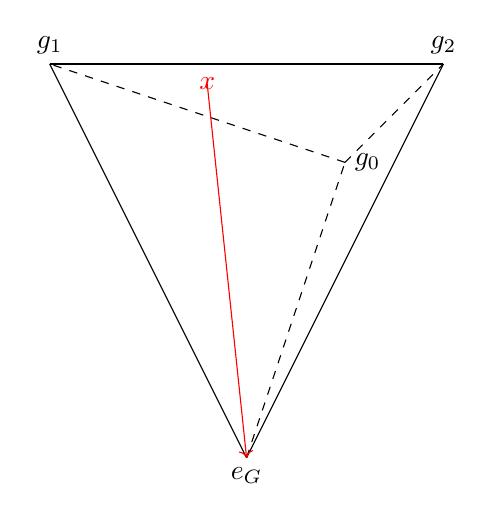
\begin{tikzpicture}[scale=1.25]
  \draw[dashed]
    (0,0) node[below] {$e_{G}$}
    --
    (1,3) node[right] {$g_{0}$};
  \draw
    (0,0)
    --
    (-2,4) node[above] {$g_{1}$};
  \draw
    (0,0)
    --
    (2,4) node[above] {$g_{2}$};
  \draw
    (-2,4)
    --
    (2,4);
  \draw[dashed]
    (1,3)
    --
    (-2,4);
  \draw[dashed]
    (1,3)
    --
    (2,4);
  \draw[->,red]
    (-0.4,3.8) node {$x$}
    --
    (0,0);
\end{tikzpicture}
\]
Note that in the case $e_{G} = g_{0}$ we get a loop in this example. Secondly, the notation  $\mathrm{E}G \slash G$ is not an unfortunate coincidence with that of the orbit space of a group action. For if we topologize $G$ by its power set and $\sim$ is the equivalence relation resulting from the continuous action $\ell_{\mathbf{Top}}$ induced by $\vert \cdot \vert \circ \ell$ then
\begin{align*}
  \mathrm{E}G
  \slash
  G
  &=
  \mathrm{E}G
  \slash
  \sim
\end{align*}
$\ell_{\mathbf{Top}}$ is a \textit{covering space action}\footnote{some say properly discontinuous action} on $\mathrm{E}G$. Since $\mathrm{E}G$ is contractible this means:
\begin{enumerate}
\item[$\bullet$]
the quotient map $\pi_{\ell_{\mathbf{Top}}}$ from $\mathrm{E}G$ to $\mathrm{E}G \slash \sim$ is a \textit{universal}\footnote{this has, in fact, to do with the notion from section \ref{sec:uni}} cover of $\mathrm{E}G \slash \sim$ with discrete fiber $G$ - that is, one whose total space is simply-connected which in turn means the $0$-th and $1$-st homotopy groups are trivial - since $\mathrm{E}G$ as contractible space is clearly simply connected
\item[$\bullet$]
$G$ is isomorphic to the fundamental group
\begin{align*}
  \pi_{1}(\mathrm{E}G \slash G)
  &\cong
  \pi_{1}(\mathrm{B}G)
\end{align*}
\end{enumerate}
This is covering space theory is nicely discussed in \cite{8b5861fc}, for example. The discreteness of the fiber plus the contractibility of the total space of $\pi_{\ell_{\mathbf{Top}}}$ imply that
\begin{align*}
  \pi_{n}(\mathrm{E}G \slash G)
\end{align*}
is trivial for $n > 1$ by a \textit{long exact sequence for Serre fibrations} argument also contained in \cite{8b5861fc}. Since $\mathrm{E}G \slash G$ is path-connected - any two points are connected by a path - the only non-trivial homotopy group of $\mathrm{B}G$ is the first and hence $\mathrm{B}G$ is what is called an \textit{Eilenberg-Mac Lane space for $(G,1)$}. Now what we have done here to understand $\mathrm{B}G$ is the so-called {\glqq}bar construction{\grqq} for a group $G$ by emulating the discussion in \cite{8b5861fc} example 1B.7 which essentially does the same as we do for strict simplicial sets. What is not directly contained there is that $\mathrm{B}G$ is an interesting classifying space\footnote{note the discussion in section \ref{sec:uni} about this terminology}. To this end note that $\pi_{\ell_{\mathbf{Top}}}$ is a locally trivial fiber bundle with fiber (the discrete group) $G$ over the orbit space $\mathrm{E}G \slash G$ resulting from a free continuous action $\ell_{\mathbf{Top}}$ by $G$ on the total space $\mathrm{E}G$ which acts clearly transitively on the fiber since the base space is the quotient space. Thus $\ell_{\mathbf{Top}}$ is a $G$-principal bundle. And this is what $\mathrm{B}G$ can be shown to classify. Namely: homotopy classes of continuous functions from some CW complex $X$ to $\mathrm{B}G$ (which is also a CW complex by theorem \ref{thm:ssetcwcompex}) correspond to isomorphism classes of $G$-principal bundles over $X$. We do not show this here. But it is an easy consequence of a fact proven in \cite{4dc38f27} which in particular implies that $G$-principal bundles with contractible total space are universal elements. The theorem from \cite{4dc38f27} we are talking about more generally applies to arbitrary topological groups and the harder part is in fact to find a universal element for such a topological group. We partly solved this task essentially with categorical means for groups with the discrete topology here. Let us now clearly formulate the statement for general topological groups and refer to proofs:
\\
\begin{thm}
\label{thm:repofbundlefunc}
Assume a group object $G$ in $\mathbf{Top}$ and define the functor
\begin{align*}
  \mathcal{P}_{G}
  \colon
  \left(
    \mathbf{HTop}^{\textrm{CW}}
  \right)^{\mathrm{op}}
  &\rightarrow
  \mathbf{Set}
\end{align*}
by
\begin{enumerate}
\item[$\bullet$]
mapping CW complexes $X$ to the set of isomorphism classes\footnote{the equivalence class w.r.t. the equivalence relation of being an isomorphism} of $G$-principal bundles with base space $X$
\item[$\bullet$]
mapping homotopy classes $[f_{12}] \colon X_{1} \rightarrow X_{2}$ to the isomorphism class of the pullback bundle $f_{12}^{\ast}(p)$ of $[p] \in \mathcal{P}_{G}(X_{2})$ along $f_{12}$
\end{enumerate}
Then $\mathcal{P}_{G}$ is representable.
\end{thm}
\begin{prf}
As pointed out this is proven in \cite{4dc38f27}. But it might also interest you that \cite{6d9ad807} constructs a classifying space for every topological group using simplicial spaces and nerves. 
\\
\phantom{proven}
\hfill
$\square$
\end{prf}
We want to emphasize that $\mathrm{hom}_{\mathbf{HTop}^{\textrm{CW}}}(\cdot,\mathrm{B}G)$ should remind us of cohomology in the light of example \ref{exa:loopradjoint}. And, in fact, $\mathrm{B}G$ is part of a certain $\Omega$-spectrum. But we do not want to elaborate on that further at this point. After all, we call $\mathrm{B}$ the \textbf{classifying space functor} and
\begin{align*}
  \mathrm{B}
  \mathbf{C}
  &\doteq
  \mathrm{B}(\mathbf{C})
\end{align*}
the \textbf{(categorical) classifying space (of $\mathbf{C}$)}. Besides that this generalizes classifying space for $G$-principal bundles with $G$ a discrete space in a canonical way (why should we restrict ourselves to delooping groupoids and not allow arbitrary categories?) we cannot directly be sure that $\mathrm{B}\mathbf{C}$ classifies a sensible mathematical construction in general and thus deserves the terminology. But there seems to be a more or less useful notion which is a certain kind of torsor. So we opted for this terminology here.
\\
To finally convince the reader of the (mathematical) importance of the classifying space functor we want to remark that $\pi_{n} \circ B$ - $\pi_{n}$ is the $n$-th homotopy group functor - applied to a certain kind of category (capturing some properties of exact sequences) is the $n$-the K-group of Quillens algebraic K-theory which is of major importance in algebraic geometry.
\\\\
Lastly, one might wonder why the nerve is called nerve and if you know cohomology you may know that this terminology is also used when it comes to what is traditionally called \v{C}ech cohomology. In fact, our nerve yields the one there more or less directly. According to \cite{wiki-nlab0000} the nerve functor $\mathrm{n}$ is due to Grothendieck who abstracted the so-called \textit{nerve of an open cover} which we will however call \textit{Alexandrov nerve} for reasons of clarity and comprehensibility since from our perspective the \textit{nerve of an open cover} would rather be
\begin{align*}
  \mathrm{n}
  \left(
    \mathbf{Open}_{S}^{\mathrm{cov}_{S}}
  \right)
\end{align*}
But this does not seem to be quite directly what Alexandrov meant.\footnote{though this is claimed in \cite{wiki-pedia0en}:nerve (category theory)} Yet it seems that the \textit{Alexandrov nerve} can in some sense be obtained as nerve in almost this way. Moreover it can be obtained from the \textit{(\v{C}ech) nerve} which is a sort of a nerve in our sense but in a more general setting. You see, things are complicated here and we think literature is quite Kafkaesque on this subject. Especially relating the \v{C}ech nerve to the traditional idea seems hard to find explicitly in literature (as far as we know) and for the sake of simplicity we will not discuss it at this point. But we try to tidy up the rest a bit as far as our understanding allows. So let $S$ be a topological space and
\begin{align*}
  \mathrm{cov}_{S}
  \colon
  K
  &\rightarrow
  \mathrm{ob}_{\mathbf{Open}_{S}}
\end{align*}
be an open cover generator for what follows.
\\
First of all we call
\begin{align*}
  \mathrm{n}
  \left(
    \mathbf{Open}_{S}^{\mathrm{cov}_{S}}
  \right)
\end{align*}
\textbf{nerve (of $\mathrm{cov}_{S}$)} though we will not use this a bit misleading terminology much.
\\
Secondly, we want to introduce the Alexandrov nerve of an open cover which is what is actually called nerve of an open cover. This seems to be historically the first idea which was referred to as nerve of something. The idea is to use $\mathrm{cov}_{S}$ to find a good combinatorial approximation of $S$. More precisely, what Alexandrov seems to have invented is a \textit{(combinatorial) simplicial complex} with vertices ($0$-simplices) just the members of the cover, that is, a vertex for each $k \in K$ or better say $U_{k} \doteq \mathrm{cov}_{S}(k)$. Next take for each non-empty intersection $U_{k_{1}} \cap U_{k_{2}}$ of cover members such that $U_{k_{1}} \neq U_{k_{2}}$ an edge ($1$-simplex) and carry on like that for higher simplices. This is to say for each $n \in \mathbb{N}$ the set of $n$-simplices shall be in bijective correspondence to the set
\begin{align*}
  F_{n}^{\mathrm{cov}_{S}}
  &:=
  \left\lbrace
      U
      \in
      \mathfrak{T}_{S}
    \,
    \vert
    \,
      \exists
      k_{1},
      \ldots
      k_{n+1}
      \in
      K
      \text{ such that }
      U
      =
      U_{k_{1}}
      \cap
      \cdots
      \cap
      U_{k_{n+1}}
      \neq
      \emptyset
      \text{ and }
      U_{k_{1}}
      \neq
      \cdots
      \neq
      U_{k_{n+1}}
  \right\rbrace
\end{align*}
If one knows what a \textit{(combinatorial) simplicial complex} is it is not too hard to see that this defines one. But actually the reader is not expected to know this. Let us geometrically allude to what this means for low dimensional simplices. Namely for vertices, edges and triangles which is sometimes also referred to as $2$-skeleton of the simplicial complex. The dotted area is the simplicial complex corresponding to the space covered by the disks delimited by the circles.
\[
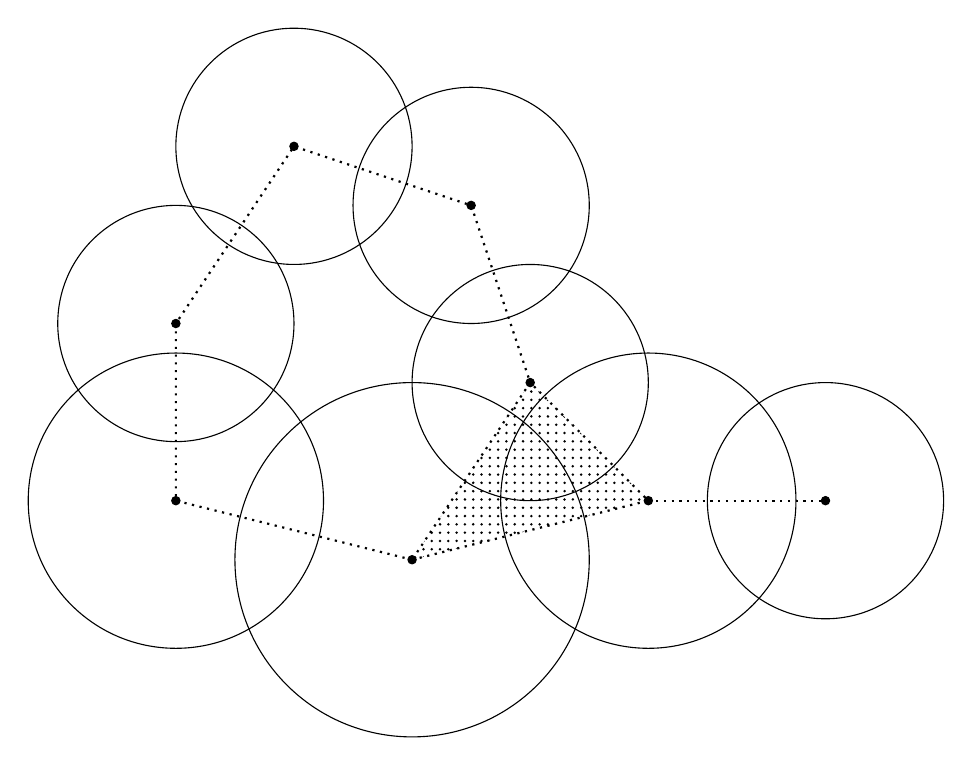
\begin{tikzpicture}[scale=0.75]
  \coordinate (u1) at (0,-1);
  \coordinate (u2) at (-4,0);
  \coordinate (u3) at (-4,3);
  \coordinate (u4) at (-2,6);
  \coordinate (u5) at (1,5);
  \coordinate (u6) at (2,2);
  \coordinate (u7) at (4,0);
  \coordinate (u8) at (7,0);
  \draw[dotted,line width=0.8pt]
    (u1)
    --
    (u2)
    --
    (u3)
    --
    (u4)
    --
    (u5)
    --
    (u6);
  \draw[pattern=dots,dotted,line width=0.8pt]
    (u1)
    --
    (u7)
    --
    (u6)
    --
    (u1)
    --
    cycle;
  \draw[dotted,line width=0.8pt]
    (u7)
    --
    (u8);
  \draw
    (u1)
    circle
    [radius=3];
  \draw
    (u2)
    circle
    [radius=2.5];
  \draw
    (u3)
    circle
    [radius=2];
  \draw
    (u4)
    circle
    [radius=2];
  \draw
    (u5)
    circle
    [radius=2];
  \draw
    (u6)
    circle
    [radius=2];
  \draw
    (u7)
    circle
    [radius=2.5];
  \draw
    (u8)
    circle
    [radius=2];
  \filldraw
    (u1)
    circle
    [radius=2pt];
  \filldraw
    (u2)
    circle
    [radius=2pt];
  \filldraw
    (u3)
    circle
    [radius=2pt];
  \filldraw
    (u4)
    circle
    [radius=2pt];
  \filldraw
    (u5)
    circle
    [radius=2pt];
  \filldraw
    (u6)
    circle
    [radius=2pt];
  \filldraw
    (u7)
    circle
    [radius=2pt];
  \filldraw
    (u8)
    circle
    [radius=2pt];
\end{tikzpicture}
\]
Since the circles and all the overlaps of the circles are contractible the geometric simplicial complex has the same homotopy type as the space covered by the circles. Open covers with this contractibility feature are often called \textit{good covers} and the theorem proving this a (weak) homotopy equivalence is often called \textit{nerve theorem}. So depending on the quality of the open cover (and perhaps the space) the \textit{simplicial complex} is a more or less good combinatorial model of the space's homotopy type. This is nice. But we actually want a simplicial set in lieu of a \textit{simplicial complex} for several reasons:
\begin{enumerate}
\item[$\bullet$]
simplicial sets have some perks we have already discussed
\item[$\bullet$]
if we have a simplicial set it could be the nerve of some category and it will be more convenient to apply category theory
\item[$\bullet$]
some readers are perhaps not familiar with simplicial complexes
\end{enumerate}
To make the simplicial complex defined by the sets $F_{n}^{\mathrm{cov}_{S}}$ into a simplicial set modeling $S$ we could totally order the set of vertices $F_{0}^{\mathrm{cov}_{S}}$ to get a so-called \textit{ordered simplicial complex} which is nothing but a strict simplicial set.\footnote{if you do not understand how this works then \cite{4dd1b85f} should produce relief} Dropping the assumption that intersections can only involve different members of the cover yields precisely the degeneracies which we miss to get a simplicial set. Now, if the cover $\mathrm{cov}_{S}$ is finite - that is, if $K$ is finite - this is no problem. Just take the induced order from $\mathbb{N}$ used to prove that $K$ is finite. But in general we have a problem if we want to avoid the axiom of choice. The axiom of choice allows to well-order any set. The drawback is that we then do not know precisely what the simplicial set looks like. But there is a pretty cool trick to avoid the axiom of choice which will also resolve our terminological struggles a bit. Take the \textit{barycentric subdivision}\footnote{this is explained in \cite{8b5861fc}, for example} of the \textit{simplicial complex} associated to the cover generated by $\mathrm{cov}_{S}$. For our illustration this geometrically means to add vertices in every non-empty intersection illustrated by small (red) circles and edges with one end the barycenter of a triangle and the other end a vertex contained in the same triangle illustrated by thin (red) lines according to the following picture.
\[
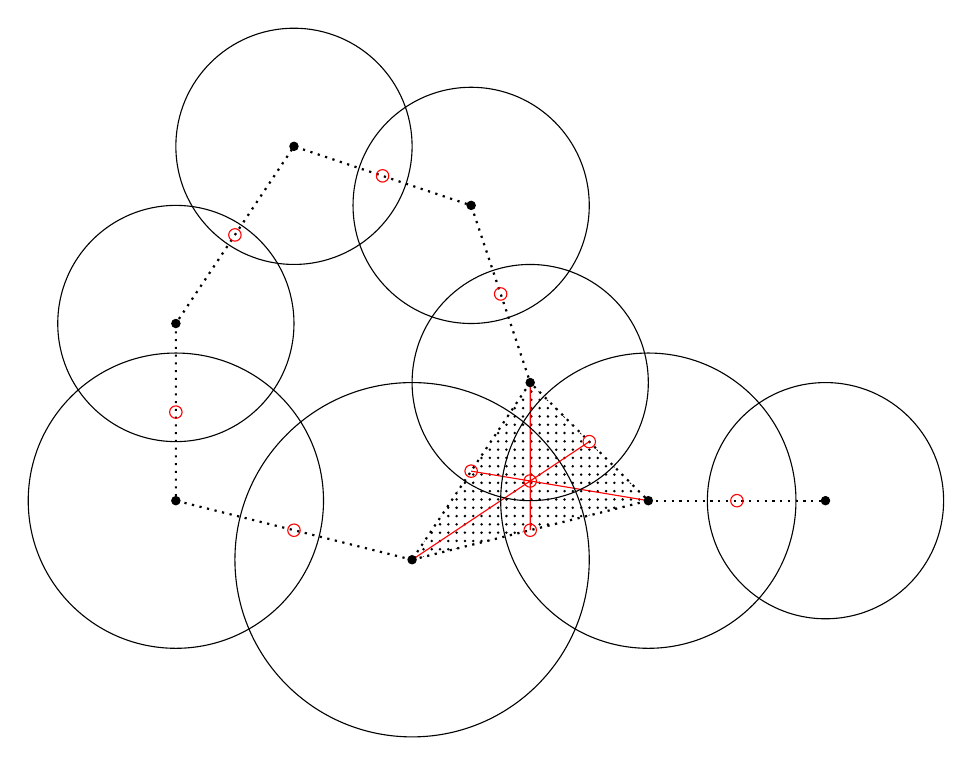
\begin{tikzpicture}[scale=0.75]
  \coordinate (u1) at (0,-1);
  \coordinate (u2) at (-4,0);
  \coordinate (u3) at (-4,3);
  \coordinate (u4) at (-2,6);
  \coordinate (u5) at (1,5);
  \coordinate (u6) at (2,2);
  \coordinate (u7) at (4,0);
  \coordinate (u8) at (7,0);
  \draw[dotted,line width=0.8pt]
    (u1)
    --
    coordinate[midway](u12)
    (u2)
    --
    coordinate[midway](u23)
    (u3)
    --
    coordinate[midway](u34)
    (u4)
    --
    coordinate[midway](u45)
    (u5)
    --
    coordinate[midway](u56)
    (u6);
  \draw[color=red]
    (u12)
    circle
    [radius=3pt];
  \draw[color=red]
    (u23)
    circle
    [radius=3pt];
  \draw[color=red]
    (u34)
    circle
    [radius=3pt];
  \draw[color=red]
    (u45)
    circle
    [radius=3pt];
  \draw[color=red]
    (u56)
    circle
    [radius=3pt];
  \draw[pattern=dots,dotted,line width=0.8pt]
    (u1)
    --
    coordinate[midway](u17)
    (u7)
    --
    coordinate[midway](u67)
    (u6)
    --
    coordinate[midway](u16)
    (u1);
  \draw[color=red]
    (barycentric cs:u1=1,u7=1,u6=1)
    circle
    [radius=3pt];
  \draw[color=red]
    (u17)
    circle
    [radius=3pt];
  \draw[color=red]
    (u67)
    circle
    [radius=3pt];
  \draw[color=red]
    (u16)
    circle
    [radius=3pt];
  \draw[thin,color=red]
    (u1)
    --
    (u67)
    (u7)
    --
    (u16)
    (u6)
    --
    (u17);
  \draw[dotted,line width=0.8pt]
    (u7)
    --
    coordinate[midway](u78)
    (u8);
  \draw[color=red]
    (u78)
    circle
    [radius=3pt];
  \draw
    (u1)
    circle
    [radius=3];
  \draw
    (u2)
    circle
    [radius=2.5];
  \draw
    (u3)
    circle
    [radius=2];
  \draw
    (u4)
    circle
    [radius=2];
  \draw
    (u5)
    circle
    [radius=2];
  \draw
    (u6)
    circle
    [radius=2];
  \draw
    (u7)
    circle
    [radius=2.5];
  \draw
    (u8)
    circle
    [radius=2];
  \filldraw
    (u1)
    circle
    [radius=2pt];
  \filldraw
    (u2)
    circle
    [radius=2pt];
  \filldraw
    (u3)
    circle
    [radius=2pt];
  \filldraw
    (u4)
    circle
    [radius=2pt];
  \filldraw
    (u5)
    circle
    [radius=2pt];
  \filldraw
    (u6)
    circle
    [radius=2pt];
  \filldraw
    (u7)
    circle
    [radius=2pt];
  \filldraw
    (u8)
    circle
    [radius=2pt];
\end{tikzpicture}
\]
The point is that the barycentric subdivision of a simplicial complex does not change its homotopy type and that to each intersection of distinct cover members there is a corresponding unique vertex of the barycentric subdivision of the simplicial complex in such a way that for any two vertices connected by an edge precisely one of them correponds to an intersection which can be included in the cover member corresponding to the other vertex. And this inclusion can be used to say which vertex is {\glqq}smaller{\grqq}. We claim the natural convention is that the vertex corresponding to the smaller (as a subset) set is the smaller vertex and indicate this by an arrow $\rightarrow$ which means ordered by inclusion in the following picture.
\[
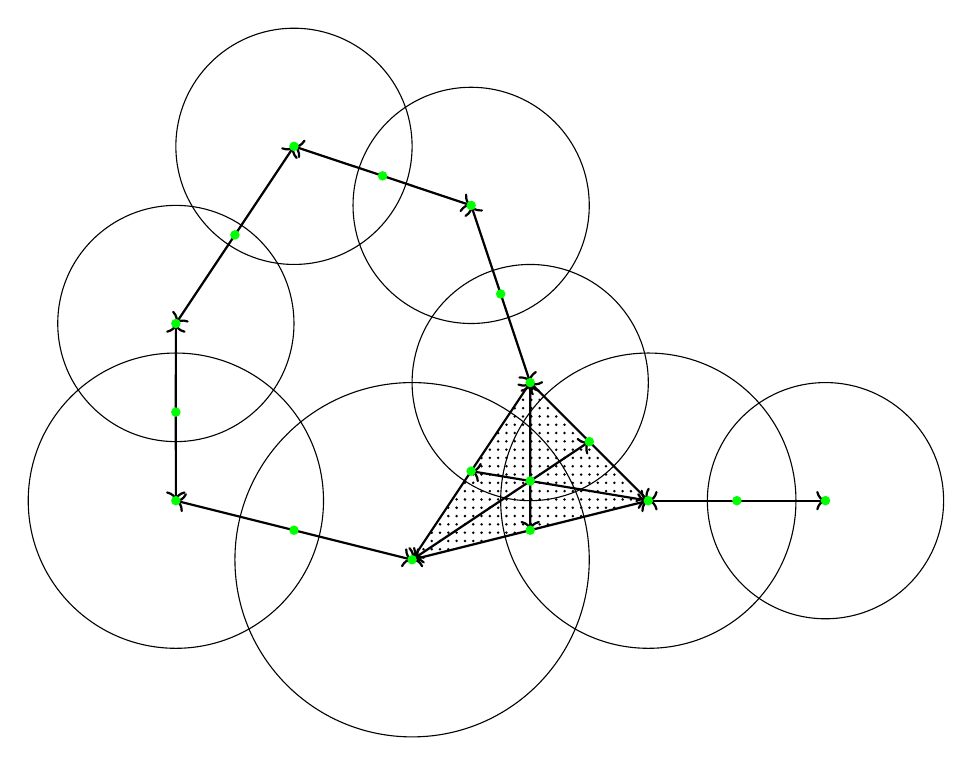
\begin{tikzpicture}[scale=0.75]
  \coordinate (u1) at (0,-1);
  \coordinate (u2) at (-4,0);
  \coordinate (u3) at (-4,3);
  \coordinate (u4) at (-2,6);
  \coordinate (u5) at (1,5);
  \coordinate (u6) at (2,2);
  \coordinate (u7) at (4,0);
  \coordinate (u8) at (7,0);
  \draw[color=white]
    (u1)
    --
    coordinate[midway](u12)
    (u2)
    --
    coordinate[midway](u23)
    (u3)
    --
    coordinate[midway](u34)
    (u4)
    --
    coordinate[midway](u45)
    (u5)
    --
    coordinate[midway](u56)
    (u6);
  \filldraw[color=white,pattern=dots]
    (u1)
    --
    coordinate[midway](u17)
    (u7)
    --
    coordinate[midway](u67)
    (u6)
    --
    coordinate[midway](u16)
    (u1);
  \draw[color=white]
    (u7)
    --
    coordinate[midway](u78)
    (u8);
  \draw[thick,->]
    (u12)
    --
    (u1);
  \draw[thick,->]
    (u12)
    --
    (u2);
  \draw[thick,->]
    (u23)
    --
    (u2);
  \draw[thick,->]
    (u23)
    --
    (u3);
  \draw[thick,->]
    (u34)
    --
    (u3);
  \draw[thick,->]
    (u34)
    --
    (u4);
  \draw[thick,->]
    (u45)
    --
    (u4);
  \draw[thick,->]
    (u45)
    --
    (u5);
  \draw[thick,->]
    (u56)
    --
    (u5);
  \draw[thick,->]
    (u56)
    --
    (u6);
  \draw[thick,->]
    (u67)
    --
    (u6);
  \draw[thick,->]
    (u67)
    --
    (u7);
  \draw[thick,->]
    (u78)
    --
    (u7);
  \draw[thick,->]
    (u78)
    --
    (u8);
  \draw[thick,->]
    (u16)
    --
    (u1);
  \draw[thick,->]
    (u16)
    --
    (u6);
  \draw[thick,->]
    (u17)
    --
    (u1);
  \draw[thick,->]
    (u17)
    --
    (u7);
  \draw[thick,->]
    (barycentric cs:u1=1,u7=1,u6=1)
    --
    (u1);
  \draw[thick,->]
    (barycentric cs:u1=1,u7=1,u6=1)
    --
    (u6);
  \draw[thick,->]
    (barycentric cs:u1=1,u7=1,u6=1)
    --
    (u7);
  \draw[thick,->]
    (barycentric cs:u1=1,u7=1,u6=1)
    --
    (u67);
  \draw[thick,->]
    (barycentric cs:u1=1,u7=1,u6=1)
    --
    (u16);
  \draw[thick,->]
    (barycentric cs:u1=1,u7=1,u6=1)
    --
    (u17);
  \draw
    (u1)
    circle
    [radius=3];
  \draw
    (u2)
    circle
    [radius=2.5];
  \draw
    (u3)
    circle
    [radius=2];
  \draw
    (u4)
    circle
    [radius=2];
  \draw
    (u5)
    circle
    [radius=2];
  \draw
    (u6)
    circle
    [radius=2];
  \draw
    (u7)
    circle
    [radius=2.5];
  \draw
    (u8)
    circle
    [radius=2];
  \filldraw[color=green]
    (u1)
    circle
    [radius=2pt];
  \filldraw[color=green]
    (u2)
    circle
    [radius=2pt];
  \filldraw[color=green]
    (u3)
    circle
    [radius=2pt];
  \filldraw[color=green]
    (u4)
    circle
    [radius=2pt];
  \filldraw[color=green]
    (u5)
    circle
    [radius=2pt];
  \filldraw[color=green]
    (u6)
    circle
    [radius=2pt];
  \filldraw[color=green]
    (u7)
    circle
    [radius=2pt];
  \filldraw[color=green]
    (u8)
    circle
    [radius=2pt];
  \filldraw[color=green]
    (u12)
    circle
    [radius=2pt];
  \filldraw[color=green]
    (u23)
    circle
    [radius=2pt];
  \filldraw[color=green]
    (u34)
    circle
    [radius=2pt];
  \filldraw[color=green]
    (u45)
    circle
    [radius=2pt];
  \filldraw[color=green]
    (u56)
    circle
    [radius=2pt];
  \filldraw[color=green]
    (u67)
    circle
    [radius=2pt];
  \filldraw[color=green]
    (u78)
    circle
    [radius=2pt];
  \filldraw[color=green]
    (u16)
    circle
    [radius=2pt];
  \filldraw[color=green]
    (u17)
    circle
    [radius=2pt];
  \filldraw[color=green]
    (barycentric cs:u1=1,u7=1,u6=1)
    circle
    [radius=2pt];
\end{tikzpicture}
\]
So the barycentric subdivision yields a strict simplicial set which when realized geometrically exhibits the same homotopy type as the geometric simplicial complex. Again, dropping the assumption that intersections can only involve different members of the cover should yield the wanted simplicial set.
\\
We hope you got the gist from this motivational discussion and hope you are able to comprehend the following definitions. From the open cover generator $\mathrm{cov}_{S}$ we get an open cover of $S$ by
\begin{align*}
  \mathfrak{D}_{\mathrm{cov}_{S}}
  &:=
  \left\lbrace
      U
      \in
      \mathfrak{T}_{S}
    \,
    \vert
    \,
      \exists
      n
      \in
      \mathbb{N}^{\times}
      \left(
        \exists
        k_{1},
        \ldots
        k_{n+1}
        \in
        K
        \text{ such that }
        U
        =
        U_{k_{1}}
        \cap
        \cdots
        \cap
        U_{k_{n+1}}
        \neq
        \emptyset
      \right)
  \right\rbrace
\end{align*}
and hence an open cover generator
\begin{align*}
  \cap_{\mathrm{cov}_{S}}
  &:=
  \mathrm{cov}_{S}
  \left[
    \mathfrak{D}_{\mathrm{cov}_{S}}
  \right]
\end{align*}
Then we call
\begin{align*}
  \mathrm{A}_{\mathrm{cov}_{S}}
  &:=
  \mathrm{n}
  \left(
    \mathbf{Open}_{S}^{\cap_{\mathrm{cov}_{S}}}
  \right)
\end{align*}
\textbf{Alexandrov nerve (of $\mathrm{cov}_{S}$)}. We claim that the geometric realization of the Alexandrov nerve is structurally equal to the simplicial set we discussed in the motivation justifying the terminology. But we do not prove that here. However, we tell you that this claim is essentially made by Segal in \cite{6d9ad807}. Unfortunately, in these notes the claim is not explained and we could not further follow back that claim to its origin. So you are on your own for a proof of this.
\\
We already indicated that covers with every member contractible are good in the sense that they may allow a \textit{nerve theorem}. Intuitively, we think this is clear from our drawings above. So let us formalize the notion of good covers. $\mathrm{cov}_{S}$ is called a \textbf{good cover (of $S$)} if any object
\begin{align*}
  U
  &\in
  \mathrm{ob}_{\mathbf{Open}_{S}^{\cap_{\mathrm{cov}_{S}}}}
\end{align*}
is contractible.
\\
Now if one has a simplicial set it is almost mandatory to apply simplicial (co)homology to examine the homotopy properties of its geometric realization. We presuppose a knowledge about simplicial homology and simplicial cohomology for simplicial sets which is essentially the same as the version for strict simplicial sets presented in \cite{8b5861fc}. Moreover we require the reader to be familiar with intuition about cohomology for what follows. See the introduction to chapter 3 of \cite{8b5861fc} to get a feeling for cocycles and coboundaries in low dimensions. You can also look at the according chapter of \cite{00000011} for a quick introduction. Now, to us only the simplicial cohomology matters. So let us briefly revisit what the simplicial cohomology for the Alexandrov nerve of $\mathrm{cov}_{S}$ is. An element of
\begin{align*}
  \mathrm{A}_{\mathrm{cov}_{S}}
  ([N])
\end{align*}
for $N \in \mathbb{N}$ is called \textbf{$N$-simplex (of $\mathrm{cov}_{S}$)} while we denote the free abelian group with generators the $N$-simplices by $\Delta_{N}[S]$ for $N \in \mathbb{N}$. Then for an $N$-simplex $\sigma$ we call
\begin{align*}
  \partial
  \sigma
  &=
  \Sigma_{i=0}^{N}
  (-1)^{i+1}
  d_{N,i}(\sigma)
\end{align*}
regarded as element of $\Delta_{N-1}[S]$ where $d_{N,i}$ is $i$-th face map of the $N$ simplices in
\begin{align*}
  \mathrm{A}_{\mathrm{cov}_{S}}
\end{align*}
the \textbf{boundary of $\sigma$}. The boundaries of all the $N$-simplices define a homomorphism $\partial_{N}$ on all of $\Delta_{N}[S]$ since it suffices to determine a homomorphism on generators. We call $\partial_{N}$ the \textbf{$N$-boundary operator} Then for some abelian group $A$ the contravariant hom-functor
\begin{align*}
  \partial^{N}
  \doteq
  \partial_{A}^{N}
  :=
  \mathrm{hom}_{\mathbf{Ab}}(\partial_{N+1},A)
  \colon
  \mathrm{mor}_{\mathbf{Ab}}
  \left(
    \Delta_{N}[S],
    A
  \right)
  &\rightarrow
  \mathrm{mor}_{\mathbf{Ab}}
  \left(
    \Delta_{N+1}[S],
    A
  \right)
\end{align*}
is called \textbf{$N$-coboundary operator}. The abelian groups
\begin{align*}
  \mathrm{mor}_{\mathbf{Ab}}
  \left(
    \Delta_{N}[S],
    A
  \right)
\end{align*}
define a cochain complex with cohomology groups
\begin{align*}
  \check{H}_{A}^{N}
  \left(
    \mathrm{A}_{\mathrm{cov}_{S}}
  \right)
  &:=
  \mathrm{ker}
  \left(
    \partial^{N}
  \right)
  \slash
  \mathrm{im}
  \left(
    \partial^{N-1}
  \right)
\end{align*}
for $N \in \mathbb{N}^{\times}$ and
\begin{align*}
  \check{H}_{A}^{0}
  \left(
    \mathrm{A}_{\mathrm{cov}_{S}}
  \right)
  &:=
  \mathrm{ker}
  \left(
    \partial^{0}
  \right)
\end{align*}
where $\mathrm{ker}$ and $\mathrm{im}$ mean \textit{kernel} and \textit{image}, respectively. For $N \in \mathbb{N}$ 
\begin{align*}
  \check{H}_{A}^{N}
  \left(
    \mathrm{A}_{\mathrm{cov}_{S}}
  \right)
\end{align*}
is called \textbf{$N$-th \v{C}ech cohomology group (of $\mathrm{cov}_{S}$ with coefficients in $A$)}. So far, so good. But we actually want a cohomology for $S$ and not for its cover. So what are our options? By the nerve theorem we should get a reasonable cohomology if we take a cover fulfilling the conditions of the nerve theorem. So the \v{C}ech cohomology group for a good cover should in certain cases yield some homotopy properties of $S$. But there is another more indirect approach. In subsection \ref{sec:func} we have said that open covers are ordered as directed set by refinement. So we can take the colimit since $\mathbf{Ab}$ is bicomplete. This is to say we can consider
\begin{align*}
  \check{H}_{A}^{N}
  \left(
    S
  \right)
  &:=
  \varinjlim_{\pmb{\leq}_{\mathrm{Cov}_{S}}}
  \left(
    \check{H}_{A}^{N}
    \left(
      \mathrm{A}_{\mathrm{cov}_{S}}
    \right)
  \right)
\end{align*}
for all $N \in \mathbb{N}$ which we call the \textbf{$N$-th \v{C}ech cohomology group (of $S$ with coefficients in $A$)}. The idea is that the Alexandrov nerve of finer and finer covers eventually is a good approximation of $S$.
\begin{align*}
  \check{H}_{A}^{N}
  \left(
    S
  \right)
\end{align*}
defines an \textit{axiomatic cohomology theory}. It is a well-known fact that for $S$ a CW complex
\begin{align*}
  \check{H}_{A}^{N}
  \left(
    S
  \right)
\end{align*}
is the same as \textit{singular cohomology for $S$ with coefficients in $A$} when compared as axiomatic cohomology theory on this category of nice spaces. Furthermore for $S \in \mathrm{ob}_{\mathbf{Diff}_{\infty}}$ the same is true for \textit{de Rham cohomology for $S$ with coefficients in $\mathbb{R}$}. But note that in the de Rham case we could also use the option of a good cover and its \v{C}ech cohomology since a smooth manifold is locally contractible and hence allows for a good cover. Therefore we want to emphasize that the colimit option is not necessarily better than the good cover option. Indeed, when considering cohomology more generally in the modern $(\infty,1)$-category context the good cover option seems more prevalent. At least when following \cite{a565d200}. There it also becomes clear that \v{C}ech cohomology is more like a method to calculate other cohomologies as we tried to suggest by relating it to singular and de Rham cohomology. Let us give a foretaste of what we mean. Above in theorem \ref{thm:repofbundlefunc} we had that isomorphism classes of $G$-principal bundles over some CW Complex $S$ are classified by morphisms from $S$ into the Eilenberg-Mac Lane space $\mathrm{B}G$. These morphisms in turn can be shown to correspond to the elements of the first singular cohomology for $S$ with coefficients $G$ if $G$ is an abelian group by the machinery alluded to in example \ref{exa:loopradjoint} (when taking base points into account). Hence the first \v{C}ech cohomology can be used to classify the addressed bundles over $S$. Therefore it seems instructive to take a closer look at
\begin{align*}
  \check{H}_{A}^{N}
  \left(
    \mathrm{A}_{\mathrm{cov}_{S}}
  \right)
\end{align*}
Well, an abelian group homomorphism
\begin{align*}
  \phi
  \colon
  \Delta_{1}[S]
  &\rightarrow
  A
\end{align*}
is precisely a $1$-cocycle (that is, an element of the kernel of $\partial^{1}$) if for any\footnote{note that $\sigma$ here is rather for \underline{s}implex than for \underline{s}ection and in the light of example \ref{exa:bundles2} an unfortunate coincidence}
\begin{align*}
  \sigma
  &\in
  \mathrm{A}_{\mathrm{cov}_{S}}
  ([2])
\end{align*}
we have
\begin{align*}
  \phi
  \left(
    d_{2,2}(\sigma)
  \right)
  =
  &\phi
  \left(
    d_{2,3}(\sigma)
  \right)
  \cdot_{A}
  \phi
  \left(
    d_{2,1}(\sigma)
  \right)
\end{align*}
which is sometimes referred to as ($1$-)cocycle condition\footnote{here is where it is worthwhile to know the motivation for cohomology \cite{8b5861fc}}. Let us emphasize that we also had that in our bundles 2 example \ref{exa:bundles2}. The first cohomology class is obtained by identifying $1$-cocycles $\phi$ and $\phi^{\backprime}$ if there is a $0$-cocycle
\begin{align*}
  a
  \colon
  \Delta_{0}[S]
  &\rightarrow
  A
\end{align*}
such that
\begin{align*}
  \phi(\sigma)
  &=
  \phi^{\backprime}(\sigma)
  \cdot_{A}
  \left(
    \partial^{0}
    \left(
      a
    \right)
  \right)
  (\sigma)
\end{align*}
for all
\begin{align*}
  \sigma
  &\in
  \mathrm{A}_{\mathrm{cov}_{S}}
  ([1])
\end{align*}
which can equivalently be expressed as
\begin{align*}
  \phi(\sigma)
  &=
  \phi^{\backprime}(\sigma)
  \cdot_{A}
  a
  \left(
    d_{1,1}(\sigma)
    -
    d_{1,0}(\sigma)
  \right)
\end{align*}
which in turn is the same as
\begin{align*}
  a
  \left(
    d_{1,0}(\sigma)
  \right)
  \cdot_{A}
  \phi(\sigma)
  &=
  \phi^{\backprime}(\sigma)
  \cdot_{A}
  a
  \left(
    d_{1,1}(\sigma)
  \right)
\end{align*}
since $A$ is abelian. We identify this as the formal coboundary condition from example \ref{exa:bundles2}. The idea now is, since we treat the space $S$ by coverings, to take the coefficients only locally to get a finer notion of \v{C}ech cohomology. For a consistent choice of local coefficients it seems reasonable to take a sheaf of coefficients. This is to say an \textit{abelian} group object in $\mathbf{Sh}(S)$. It is not much trouble to make this work to yield a more general version of the \v{C}ech cohomology we presented here. The ordinary case is contained as the special case with the so-called \textit{contant sheaf (on $S$ determined by $A$)} in the more general one. By constant sheaf we just mean the sheafification (see example \ref{exa:sheafetale}) of the presheaf which maps any open subspace of $S$ to $A$ while restriction is just identity. One only has to take care of restrictions along inclusions a bit. How this works in detail can be found on \cite{wiki-pedia0en}: \v{C}ech cohomology. We will only look at the case of the first \v{C}ech cohomology group in the more general non-abelian case. This non-abelian (\v{C}ech) cohomology is important since for $G$-principal bundles $G$ is in general not abelian. What we essentially do to generalize first \v{C}ech cohomology is replacing the topological group $G$ by a group object in $\mathbf{Sh}(S)$ which is then a generalized space. Hence a final example for this section prolonging the generalized spaces example from examples \ref{exa:gs1} and \ref{exa:gs2}.
\\
\begin{exa}[Generalized Spaces III]
\label{exa:gs3}
In the following assume that $G$ is a group object in $\mathbf{Sh}(S)$ w.r.t. some $(\mathrm{m},\mathrm{id},\mathrm{inv})$. This in particular means that we locally have groups
\begin{align*}
  \left(
    G(U),
    \mathrm{m}(U),
    \mathrm{id}(U),
    \mathrm{inv}(U)
  \right)
\end{align*}
for $U \in \mathrm{ob}_{\mathbf{Open}_{S}}$. But for different objects $U_{1},U_{2} \in \mathrm{ob}_{\mathbf{Open}_{S}}$ we do not necessarily have that $G(U_{1})$ equals $G(U_{2})$ we only have a restriction (in the guise of a group homomorphism) from $G(U_{2})$ to $G(U_{1})$ if and only if $U_{1} \subset U_{2}$. Thus the cocycle condition does not quite make sense directly anymore since each term of this condition is potentially in a different group and we should restrict the terms to the largest possible common domain, that is, the intersection of all the domains involved. So let
\begin{align*}
  \sigma
  &\in
  \mathrm{A}_{\mathrm{cov}_{S}}([2])
\end{align*}
Note that $\sigma$ is a functor on $\pmb{\leq}_{[2]}$ and hence use the notation
\begin{align*}
  U_{k}
  &\doteq
  \sigma(k)
  \in
  \mathrm{ob}_{\mathbf{Open}_{S}^{\cap_{\mathrm{cov}_{S}}}}
  \\
  U_{1}
  \cap_{\textrm{f}}
  U_{2}
  &\doteq
  d_{2,3}(\sigma)
  \\
  U_{2}
  \cap_{\textrm{f}}
  U_{3}
  &\doteq
  d_{2,1}(\sigma)
  \\
  U_{1}
  \cap_{\textrm{f}}
  U_{3}
  &\doteq
  d_{2,2}(\sigma)
\end{align*}
for $k = 1,2,3$ as well as
\begin{align*}
  \mathrm{i}_{1}
  &\in
  \mathrm{mor}_{\mathbf{Open}_{S}}
  \left(
    U_{1}
    \cap
    U_{2}
    \cap
    U_{3},
    U_{2}
    \cap
    U_{3}
  \right)
  \\
  \mathrm{i}_{2}
  &\in
  \mathrm{mor}_{\mathbf{Open}_{S}}
  \left(
    U_{1}
    \cap
    U_{2}
    \cap
    U_{3},
    U_{1}
    \cap
    U_{3}
  \right)
  \\
  \mathrm{i}_{3}
  &\in
  \mathrm{mor}_{\mathbf{Open}_{S}}
  \left(
    U_{1}
    \cap
    U_{2}
    \cap
    U_{3},
    U_{1}
    \cap
    U_{2}
  \right)
\end{align*}
Then we call a dependent function
\begin{align*}
  \phi
  &\in
  \prod_{\sigma^{\backprime} \in \mathrm{A}_{\mathrm{cov}_{S}}([1])}
  G(\sigma^{\backprime}(1) \cap \sigma^{\backprime}(2))
\end{align*}
a \textbf{$1$-cocycle (for $\mathrm{cov}_{S}$ with coefficients in $G$)} if
\begin{align*}
  G(\mathrm{i}_{2})
  \left(
    \phi(U_{1} \cap_{\textrm{f}} U_{3})
  \right)
  &=
  \left(
    \mathrm{m}
    \left(
      U_{1}
      \cap
      U_{2}
      \cap
      U_{3}
    \right)
  \right)
  \left(
    G(\mathrm{i}_{3})
    \left(
      \phi(U_{1} \cap_{\textrm{f}} U_{2})
    \right),
    G(\mathrm{i}_{1})
    \left(
      \phi(U_{2} \cap_{\textrm{f}} U_{3})
    \right)
  \right)
\end{align*}
which we abbreviate
\begin{align*}
  \phi(U_{1} \cap_{\textrm{f}} U_{3})
  &=
  \phi(U_{1} \cap_{\textrm{f}} U_{2})
  \phi(U_{2} \cap_{\textrm{f}} U_{3})
\end{align*}
for all
\begin{align*}
  \sigma
  &\in
  \mathrm{A}_{\mathrm{cov}_{S}}([2])
\end{align*}
Moreover we define an equivalence relation $\sim$ on the set of $1$-cocycles by
\begin{align*}
  \phi
  &\sim
  \phi^{\backprime}
\end{align*}
for
\begin{align*}
  \phi,
  \phi^{\backprime}
  &\in
  \prod_{\sigma^{\backprime} \in \mathrm{A}_{\mathrm{cov}_{S}}([1])}
  G(\sigma^{\backprime}(1) \cap \sigma^{\backprime}(2))
\end{align*}
if and only if there is
\begin{align*}
  f
  \in
  \prod_{\sigma^{\backprime} \in \mathrm{A}_{\mathrm{cov}_{S}}([0])}
  G(\sigma^{\backprime}(1))
\end{align*}
such that
\begin{align*}
  f(U_{1})
  \phi(U_{1} \cap_{\textrm{f}} U_{2})
  =
  \phi^{\backprime}(U_{1} \cap_{\textrm{f}} U_{2})
  f(U_{2})
\end{align*}
with a simliar notational convention as for the cocycle condition to handle restriction and multiplication economically. We have to admit that this coboundary condition is a bit arbitrarily abstracted from the constant and abelian case but we feel emboldened for this by the observations in example \ref{exa:bundles2} about the principal bundles. Moreover it seems to later fit to cohomology in the $(\infty,1)$-categorical context vindicating it a bit a posteriori or so. Either way the rest of the example works with this choice. Now what is left to make this first non-abelian \v{C}ech generalization deserving the name is to either look at good covers or let the equivalence classes vary with the directed system of covers. The first option is quite clear. For the latter define the functor
\begin{align*}
  H_{G}^{1}
  \colon
  \pmb{\leq}_{\mathrm{Cov}_{S}}
  &\rightarrow
  \mathbf{Grp}^{\mathrm{op}}
  \\
  \mathrm{cov}_{S}
  &\mapsto
  \left.
    \left(
      \prod_{\sigma^{\backprime} \in \mathrm{A}_{\mathrm{cov}_{S}}([1])}
      G(\sigma^{\backprime}(1) \cap \sigma^{\backprime}(2))
    \right)
  \right\slash
  \sim
  \\
  \left(
    \mathrm{cov}_{S}^{\alpha},
    \mathrm{cov}_{S}
  \right)
  &\mapsto
  \left(
    [\phi]
    \mapsto
    \left[
      \sigma^{\alpha}
      \mapsto
      G(\mathrm{i}_{\sigma^{\alpha},\sigma^{\backprime}})
      (\phi(\sigma^{\backprime}))
    \right]
  \right)
\end{align*}
where
\begin{align*}
  \mathrm{i}_{\sigma^{\alpha},\sigma^{\backprime}}
  &\in
  \mathrm{mor}_{\mathbf{Open}_{S}}
  \left(
    \sigma^{\alpha}(1)
    \cap
    \sigma^{\alpha}(2),
    \sigma^{\backprime}(1)
    \cap
    \sigma^{\backprime}(2)
  \right)
\end{align*}
is from a choice we can make by the refinement property. Now we can apply the colimit functor (since $\mathbf{Grp}$ is a bicomplete category) to get a generalized version of \v{C}ech cohomology. In the one-dimensional case at least. 
\begin{align*}
  \check{H}_{G}^{1}(S)
  &:=
  \varinjlim_{\pmb{\leq}_{\mathrm{Cov}_{S}}}
  \left(
    H_{G}^{1}
  \right)
\end{align*}
is called the \textbf{$1$-st \v{C}ech cohomology group (of $S$ with coefficients in $G$)}. Note that $G$ is a sheaf here as group object in the topos of sheaves $\mathbf{Sh}(S)$. What we should now do is to construct from a cocycle the thing it classifies in an intuitive manner. We are sorry that we are not able to directly do this here. We just do not know how this goes although we tried hard. Therefore we only tell you what it classifies: the $1$-st \v{C}ech cohomology group classifies isormophism classes of right $G$-torsors in $\mathbf{Sh}(S)$. For a proof sketch of this fact you can look at \cite{c82f5e22}. Note that example \ref{exa:gs4} in section \ref{sec:fibration}, the sequel to this example, is a also based on a part of \cite{c82f5e22}. Anyways, the proof sketch there utilizes the equivalence of sheaves and \'{e}tale bundles from example \ref{exa:sheafetale} which we actually wanted to avoid. Yet, we can recommend the proof to gain some insight since the perspective as bundle is not the wrong in the end. What is interesting here is that the traditional $1$-st \v{C}ech cohomology group classifies loosly speaking torsors in the slice category $\mathbf{Top} \slash S$ with a certain local triviality property while the generalized version of $1$-st \v{C}ech cohomology group classifies torsors in $\mathbf{Sh}(S)$. At first glance it seems as we somehow have forgotton the local triviality by generalizing. But note that sheaves themselves capture local triviality in some sense. That this is sensible can be seen in the case of discrete topological groups $G$ for which the $G$-principal bundles correspond to $\bar{G}$-torsors where $\bar{G}$ is the constant sheaf determined by $G$. A discussion can be found in \cite{c55c71e8} in the classifying topoi chapter.
\iffalse
Now let
\begin{align*}
  \phi
  &\in
  \prod_{\sigma^{\backprime} \in \mathrm{A}_{\mathrm{cov}_{S}}([1])}
  G(\sigma^{\backprime}(1) \cap \sigma^{\backprime}(2))
\end{align*}
be a $1$-cocycle for $\mathrm{cov}_{S}$ with coefficients in $G$. Then $\phi$ induces a bijection from $G(U_{k})$ to $G(U_{k})$ for all $k \in K$ by right multiplication with $\phi(\sigma_{k})$ where $\sigma_{k} \in \mathrm{A}_{\mathrm{cov}_{S}}([1])$ denotes the degenerate $1$-simplex for $U_{k}$, that is,
\begin{align*}
  U_{k}
  &=
  \sigma_{k}(1)
  =
  \sigma_{k}(2)
\end{align*}
This is to say the function
\begin{align*}
  r_{\phi(\sigma_{k})}
  \colon
  G(U_{k})
  &\rightarrow
  G(U_{k})
  \\
  g
  &\mapsto
  g
  \cdot_{G(U_{k})}
  \phi(\sigma_{k})
\end{align*}
is a bijection.\footnote{this can be made into a group automorphism by considering $\phi(\sigma_{k})$ as identity of the codomain while the domain still has the old identity} Now let $V \subset U_{k}$ and $\mathrm{i}_{V}$ the inclusion into $U_{k}$. Then we have a group homomorphism $G(\mathrm{i}_{V})$ from $G(U_{k})$ to $G(V)$ since $G$ is a sheaf in groups. Moreover we get a bijection
\begin{align*}
  r_{G(\mathrm{i}_{V})(\phi(\sigma_{k}))}
  \colon
  G(V)
  &\rightarrow
  G(V)
  \\
  g
  &\mapsto
  g
  \cdot_{G(V)}
  G(\mathrm{i}_{V})
  \left(
    \phi(\sigma_{k})
  \right)
\end{align*}
such that
\begin{align*}
  r_{G(\mathrm{i}_{V})(\phi(\sigma_{k}))}
  \left(
    G(\mathrm{i}_{V})(g)
  \right)
  &=
  G(\mathrm{i}_{V})(g)
  \cdot_{G(V)}
  G(\mathrm{i}_{V})
  \left(
    \phi(\sigma_{k})
  \right)
  \\
  &=
  G(\mathrm{i}_{V})
  \left(
    g
    \cdot_{G(U_{k})}
    \phi(\sigma_{k})
  \right)
  \\
  &=
  G(\mathrm{i}_{V})
  \left(
    r_{\phi(\sigma_{k})}(g)
  \right)
\end{align*}
for all $g \in G(U_{k})$ since $G(\mathrm{i}_{V})$ is a group homomorphism. Thus one can show that $r_{\phi(\sigma_{k})}$ defines a sheaf isomorphism $r_{\phi}$ (natural isomorphism) from $G$ restricted to $\mathbf{Open}_{U_{K}}$ to itself by setting
\begin{align*}
  r_{\phi}(V)
  &:=
  r_{G(\mathrm{i}_{V})(\phi(\sigma_{k}))}
\end{align*}
But this corresponds to a sheaf isomorphism $\mathsf{r}_{\phi}$ from $G$ to $G$ such that
\begin{align*}
  \mathsf{r}_{\phi}(U_{k})
  &=
  r_{\phi}(U_{k})
\end{align*}
One can see this in a quite elementary way: any $U \in \mathrm{ob}_{\mathbf{Open}_{S}}$ is covered by all the $U_{k} \cap U$ and then $\mathsf{r}_{\phi}$ is obtained from the universality of the equalizers from the descent condition symbolically illustrated by
\[
\begin{tikzcd}[sep=huge]
  G(U)
  \arrow{r}{\mathrm{eq}}
  \arrow[swap]{d}{\mathsf{r}_{\phi}(U)}
  &
  \prod_{k \in K}
  G(U_{k} \cap U)
  \arrow{d}{\prod_{k \in K}r_{\phi}(U_{k} \cap U)}
  \\
  G(U)
  \arrow{r}{\mathrm{eq}}
  &
  \prod_{k \in K}
  G(U_{k} \cap U)
\end{tikzcd}
\]
So a cocycle $\phi$ yields an isomorphism of sheaves $\mathsf{r}_{\phi}$ from $G$ to $G$ and hence actions
\begin{align*}
  \mathsf{a}_{\phi}(U)
  \colon
  G(U)
  \times
  G(U)
  &\rightarrow
  G(U)
  \\
  (g_{0},g)
  &\mapsto
  \mathsf{r}_{\phi}(U)(g)
  \cdot
  g_{0}
\end{align*}
\fi
\end{exa}
\begin{prf}
For what you do not understand we can only help you by the sources given in the example.
\\
\phantom{proven}
\hfill
$\square$
\end{prf}



\section{Fibration}
\label{sec:fibration}
%\nocite{c82f5e22}
%\nocite{78202e13}
%\nocite{ab8cfa22}
%TODO
%  the whole grothendieck construction
This section is dedicated to fibrations. Fibrations (and their duals - cofibrations) originally come from classical homotopy theory. They can be thought of a bit as homotopy-theoretic fiber bundles there with the fiber only up to homotopy. In this section we use categorical means to say what a fibration is really characterized by in our context of homotopy theory. In this context it makes also sense to discuss Grothendieck fibrations as we will see and hence the Grothendieck construction establishing an equivalence of the Grothendieck fibrations to a certain variant of functors. This is a really important part of category theory we will not fully discuss here. Important to us here is that in the end we get in some sense a $(2,1)$-categorical version of sheaves called stacks which qualify as generalized spaces. One consistency condition for stacks is formally the ($1$-)cocycle condition we know from the bundles 2 example \ref{exa:bundles2} and from the discussion of \v{C}ech cohomology in the last section \ref{sec:sset} .
\\\\
In subsubsection \ref{sec:coyoneda2} we made extensive use of the category of coelements and the projection functor $\pi_{P}$ for some presheaf $P$ on $\mathbf{J}$. This is presumably the first known Grothendieck fibration and it makes didactically sense to abstract the notion from this example. To this end note that
\begin{align*}
  \pi_{P}
  \colon
  \int_{\mathbf{J}}^{\prime}
  P
  &\rightarrow
  \mathbf{J}
  \\
  (J,z)
  &\mapsto
  J
  \\
  j_{21}^{\mathrm{op}}
  &\mapsto
  j_{12}
\end{align*}
is a functor such that for all $j_{12}$ and all $z_{2} \in P(J_{2})$ there is $P(j_{12})(z_{2}) \in P(J_{1})$ and
\begin{align*}
  j_{12}
  &\in
  \mathrm{mor}_{\int_{\mathbf{J}}^{\prime}P}
  \left(
    \left(
      J_{1},
      P(j_{12})(z_{2})
    \right),
    (J_{2},z_{2})
  \right)
\end{align*}
satisfying
\begin{enumerate}
\item[$\bullet$]
$\pi_{P}(j_{12}) = j_{12}$
\item[$\bullet$]
for any
\begin{align*}
  j_{02}
  &\in
  \mathrm{mor}_{\int_{\mathbf{J}}^{\prime}P}
  \left(
    (J_{0},z_{0}),
    (J_{2},z_{2})
  \right)
\end{align*}
and any
\begin{align*}
  j_{01}
  &\in
  \mathrm{mor}_{\mathbf{J}}
  \left(
    \pi_{P}(J_{0},z_{0}),
    J_{1}
  \right)
\end{align*}
for which
\begin{align*}
  j_{12}
  \circ
  j_{01}
  &=
  \pi_{P}(j_{02})
\end{align*}
then
\begin{align*}
  j_{01}
  &\in
  \mathrm{mor}_{\int_{\mathbf{J}}^{\prime}P}
  \left(
    (J_{0},z_{0}),
    (J_{1},P(j_{12})(z_{2}))
  \right)
\end{align*}
makes the equations
\begin{align*}
  \pi_{P}(j_{01})
  &=
  j_{01}
  \\
  j_{12}
  \circ
  j_{01}
  &=
  j_{02}
\end{align*}
true because
\begin{align*}
  \pi_{P}(j_{02})
  &=
  j_{02}
\end{align*}
and since $\pi_{P}$ is the inclusion on morphisms, $j_{01}$ is the unique arrow doing so
\end{enumerate}
If we take $\mathbf{J}$ to be a groupoid then also
\begin{align*}
  \int_{\mathbf{J}}^{\prime}
  P
\end{align*}
is a groupoid and hence it makes sense to consider the morphisms in these categories as paths. In topological language, $\pi_{P}$ then allows lifting of paths since any path $j_{12}$ is {\glqq}lifted{\grqq} for $z_{2} \in P(J_{2})$ to
\begin{align*}
  j_{12}
  &\in
  \mathrm{mor}_{\int_{\mathbf{J}}^{\prime}P}
  \left(
    \left(
      J_{1},
      P(j_{12})(z_{2})
    \right),
    (J_{2},z_{2})
  \right)
\end{align*}
such that
\begin{align*}
  \pi_{P}(j_{12})
  &=
  j_{12}
\end{align*}
And these lifted paths are universal in the sense that any other path to $(J_{2},z_{2})$ factors through them uniquely. Hence the lifts should be unique up to homotopy.
\\
Lifting can be defined categorically. Given a category $\mathbf{C}$ and objects $E,B$ as well as a morphism
\begin{align*}
  p
  &\in
  \mathrm{mor}_{\mathbf{C}}(E,B)
\end{align*}
then for a morphism
\begin{align*}
  f
  &\in
  \mathrm{mor}_{\mathbf{C}}(X_{0},B)
\end{align*}
a \textbf{lift (of $f$ by $p$)} is a morphism
\begin{align*}
  \tilde{f}
  &\in
  \mathrm{mor}_{\mathbf{C}}(X_{0},E)
\end{align*}
such that
\begin{align*}
  p
  \circ
  \tilde{f}
  =
  f
\end{align*}
The dual idea of lifting is extension: given a category $\mathbf{C}$ and objects $A,X$ as well as a morphism
\begin{align*}
  i
  &\in
  \mathrm{mor}_{\mathbf{C}}(A,X)
\end{align*}
then for a morphism
\begin{align*}
  f
  &\in
  \mathrm{mor}_{\mathbf{C}}(A,X_{0})
\end{align*}
an \textbf{extension (of $f$ by $i$)} is a morphism
\begin{align*}
  \tilde{f}
  &\in
  \mathrm{mor}_{\mathbf{C}}(X,X_{0})
\end{align*}
such that
\begin{align*}
  \tilde{f}
  \circ
  i
  =
  f
\end{align*}
$i$ and $p$ are arbitrary arrows in $\mathbf{C}$ or say objects in $\mathbf{C}_{\rightarrow}$ and we say that $p$ has the \textbf{lifting property (w.r.t. $i$)}, or equivalently, $i$ has the \textbf{extension property (w.r.t. $p$)} if for all
\begin{align*}
  (f_{1},f_{2})
  &\in
  \mathrm{mor}_{\mathbf{C}_{\rightarrow}}(i,p)
\end{align*}
there is
\begin{align*}
  \tilde{f}
  &\in
  \mathrm{mor}_{\mathbf{C}}(X,E)
\end{align*}
such that $\tilde{f}$ is a lift of $f_{2}$ by $p$ and an extension of $f_{1}$ by $i$, that is, the diagram
\[
\begin{tikzcd}[sep=large]
  A
  \arrow{r}{f_{1}}
  \arrow[swap]{d}{i}
  &
  E
  \arrow{d}{p}
  \\
  X
  \arrow{ur}{\tilde{f}}
  \arrow{r}{f_{2}}
  &
  B
\end{tikzcd}
\]
commutes.\footnote{it is common in literature to refer to the lifting property as right lifting property while to the extension property one commonly refers to as left lifting property}
\\
\begin{exa}
\label{exa:liftextintop}
To make sense of the above take $\mathbf{Top}$ as $\mathbf{C}$ and
\begin{enumerate}
\item[$\bullet$]
in the lifting case the (closed) unit interval $[0,1]$ as $X$. Then we would talk about the lift of a path or ipso facto of {\glqq}path lifting{\grqq}.
\item[$\bullet$]
in the case of extensions $i$ as inclusion. Then we would clearly extend a map.
\end{enumerate}
Now for a space $Y$ let
\begin{align*}
  i_{0}^{Y}
  \colon
  Y
  &\rightarrow
  Y
  \times
  [0,1]
  \\
  y
  &\mapsto
  (y,0)
\end{align*}
Then a map $p \colon E \rightarrow B$ which has the lifting property with respect to $i_{0}^{Y}$ for all $Y$ is called \textbf{(Hurewicz) fibration} and if it only has the lifting property w.r.t. $i_{0}^{Y}$ with $Y$ a CW complex one says that $p$ is a \textbf{Serre fibration}. On the other hand, for a space $Y$ let
\begin{align*}
  p_{0}^{Y}
  \colon
  \mathrm{mor}_{\mathbf{Top}}([0,1],Y)
  &\rightarrow
  Y
  \\
  p
  &\mapsto
  p(0)
\end{align*}
where we require $\mathrm{mor}_{\mathbf{Top}}([0,1],Y)$ to be topologized such that a function
\begin{align*}
  H
  \colon
  Y_{1}
  &\rightarrow
  \mathrm{mor}_{\mathbf{Top}}([0,1],Y_{2})
\end{align*}
is continuous if and only if the curried one is continuous. This is one reason why one demands a convenient category of spaces for the purpose of (classical) homotopy theory. Anyways, a map $i \colon A \rightarrow X$ which has the extension property with respect to $p_{0}^{Y}$ for all $Y$ is called \textbf{cofibration}. The duality between fibrations and cofibrations is sometimes referred to as Eckmann-Hilton duality.
\end{exa}
\begin{prf}
Look at \cite{8b5861fc} and \cite{78202e13} if you do not exactly know what we are talking about but want to know.
\\
\phantom{proven}
\hfill
$\square$
\end{prf}
This example \ref{exa:liftextintop} suggests to define fibration as something having the lifting property w.r.t. to a bunch of arrows and dually a cofibration as something having the extension property w.r.t. to a bunch of arrows. So let
\begin{align*}
  M
  \subset
  \mathrm{Mor}_{\mathbf{C}}
\end{align*}
Then a 
\begin{align*}
  p
  &\in
  \mathrm{mor}_{\mathbf{C}}(E,B)
\end{align*}
is called \textbf{(generalized) fibration (in $\mathbf{C}$ w.r.t $M$)} if $p$ has the lifting property w.r.t. all $m \in M$ while a 
\begin{align*}
  i
  &\in
  \mathrm{mor}_{\mathbf{C}}(A,X)
\end{align*}
is called \textbf{(generalized) cofibration (in $\mathbf{C}$ w.r.t $M$)} if $i$ has the extension property w.r.t. all $m \in M$. This definition is a little too broad for the purpose of homotopy theory. Therefore we used {\glqq}generalized{\grqq}. For fibration in the model category sense one only demands lifting w.r.t. cofibrations that are weak equivalences - so called acyclic cofibrations. And for cofibration in the model category sense one only demands extension w.r.t. fibrations that are weak equivalences - so called acyclic fibrations. In particular fibrations and cofibrations are not independent of each other.
\\
After this terminology interlude we turn back to $\pi_{P}$. Given a universe large enough we recognize $\pi_{P}$ for $\mathbf{J}$ a groupoid as a fibration in $\mathbf{Grpd}$ w.r.t. to functors $I$ which are an equivalence and for which $I_{\textrm{ob}}$ is the inclusion.\footnote{the keywords are isofibration and the canonical model structure on $\mathbf{Grpd}$} In the general case of $\pi_{P}$ a morphism in $\mathbf{Cat}$ the functor $\pi_{P}$ still satisfies some lifting property. Hence we might hope to abstract a definition for a special sort of fibration in $\mathbf{Cat}$ from $\pi_{P}$. This works and leads to the notion of Grothendieck fibration. Let $\mathbf{E}$ and $\mathbf{B}$ be small categories for the rest of this subsection. Moreover let
\begin{align*}
  \pi
  \colon
  \mathbf{E}
  &\rightarrow
  \mathbf{B}
\end{align*}
be a functor and agree to the notation
\begin{align*}
  B
  &\in
  \mathrm{ob}_{\mathbf{B}}
  \\
  E,
  E_{1},
  E_{2}
  &\in
  \mathrm{ob}_{\mathbf{E}}
\end{align*}
for the rest of this subsection. Then
\begin{enumerate}
\item[(1T)]
for
\begin{align*}
  b
  &\in
  \mathrm{mor}_{\mathbf{B}}
  \left(
    B,
    \pi(E_{2})
  \right)
\end{align*}
an arrow
\begin{align*}
  \widetilde{b}
  \in
  \mathrm{mor}_{\mathbf{E}}(E_{1},E_{2})
\end{align*}
is \textbf{(terminally $\pi$-)cartesian for $b$ and $E_{2}$} if
\begin{enumerate}
\item[(TC1)]
\begin{align*}
  \pi(\widetilde{b})
  &=
  b
\end{align*}
\item[(TC2)]
for any
\begin{align*}
  e
  &\in
  \mathrm{mor}_{\mathbf{E}}(E,E_{2})
  \\
  \pi_{e}
  &\in
  \mathrm{mor}_{\mathbf{B}}
  \left(
    \pi(E),
    B
  \right)
\end{align*}
such that
\begin{align*}
  b
  \circ
  \pi_{e}
  &=
  \pi(e)
\end{align*}
that is, such that the diagram
\[
\begin{tikzcd}[sep=large]
  &
  B
  \arrow{dr}{b}
  &
  \\
  \pi(E)
  \arrow{ur}{\pi_{e}}
  \arrow{rr}{\pi(e)}
  &
  &
  \pi(E_{2})
\end{tikzcd}
\]
commutes there is a unique
\begin{align*}
  e_{!}
  \in
  \mathrm{mor}_{\mathbf{E}}(E,E_{1})
\end{align*}
such that
\begin{align*}
  \pi(e_{!})
  &=
  \pi_{e}
  \\
  \tilde{b}
  \circ
  e_{!}
  &=
  e
\end{align*}
that is, we have the informal partly commutative diagram
\[
\begin{tikzcd}[sep=large]
  &
  E_{1}
  \arrow{dr}{\tilde{b}}
  &
  \\
  E
  \arrow{ur}{e_{!}}
  \arrow{rr}{e}
  &
  \arrow[shorten <= 10pt, shorten >= 10pt]{dd}{\pi}
  &
  E_{2}
  \\
  &
  &
  \\
  &
  B
  \arrow{dr}{b}
  &
  \\
  \pi(E)
  \arrow{ur}{\pi_{e}}
  \arrow{rr}{\pi(e)}
  &
  &
  \pi(E_{2})
\end{tikzcd}
\]
involving different categories.
\end{enumerate}
$\pi$ is a \textbf{(terminal Grothendieck) fibration} if there is a terminally $\pi$-cartesian arrow for all
\begin{align*}
  b
  &\in
  \mathrm{mor}_{\mathbf{B}}
  \left(
    B,
    \pi(E_{2})
  \right)
\end{align*}
$\mathbf{E}$ is said to be \textbf{(terminally) fibered (over $\mathbf{B}$)} if $\pi$ is a terminal Grothendieck fibration. Furthermore $\mathbf{E}$ is called \textbf{total category of $\pi$} while $\mathbf{B}$ is called \textbf{base category of $\pi$}.
\\
Since for a fibration $\pi$ we must provide a terminally $\pi$-cartesian arrow $\tilde{b}$ for all
\begin{align*}
  b
  &\in
  \mathrm{mor}_{\mathbf{B}}
  \left(
    B,
    \pi(E_{2})
  \right)
\end{align*}
there is a function mapping $(b,E_{2})$ to $\tilde{b}$, that is, we have a function
\begin{align*}
  \gamma_{\pi}
  \colon
  \left\lbrace
      (b,E_{2})
      \in
      \mathrm{Mor}_{\mathbf{B}}
      \times
      \mathrm{ob}_{\mathbf{E}}
    \,
    \vert
    \,
      \mathrm{cod}_{\mathbf{B}}(b)
      =
      \pi(E_{2})
  \right\rbrace
  &\rightarrow
  \mathrm{Mor}_{\mathbf{E}}
  \\
  (b,E_{2})
  &\mapsto
  \tilde{b}
\end{align*}
where $\tilde{b}$ denotes the same morphism as above. $\gamma_{\pi}$ is called \textbf{cleavage (for $\pi$)}. It is clear that cleavages which respect identity arrows and composition of arrows are particularly nice (as functors are). In this case one speaks of splitting. Formally, a cleavage $\gamma_{\pi}$ for $\pi$ is a \textbf{splitting (of $\pi$)} if
\begin{enumerate}
\item[(TS1)]
for $B = \pi(E_{2})$ the equation
\begin{align*}
  \gamma_{\pi}(\mathrm{id}_{B},E_{2})
  &=
  \mathrm{id}_{E_{2}}
\end{align*}
holds
\item[(TS2)]
for
\begin{align*}
  b_{1}
  &\in
  \mathrm{mor}_{\mathbf{B}}
  \left(
    B,
    \pi(E_{1})
  \right)
  \\
  b_{12}
  &\in
  \mathrm{mor}_{\mathbf{B}}
  \left(
    \pi(E_{1}),
    \pi(E_{2})
  \right)
\end{align*}
such that
\begin{align*}
  E_{1}
  &=
  \mathrm{dom}_{\mathbf{E}}
  \left(
    \gamma_{\pi}(b_{12},E_{2})
  \right)
\end{align*}
the equation
\begin{align*}
  \gamma_{\pi}(b_{12},E_{2})
  \circ
  \gamma_{\pi}(b_{1},E_{1})
  &=
  \gamma_{\pi}(b_{12} \circ b_{1},E_{2})
\end{align*}
holds
\end{enumerate}
\item[(1I)]
for
\begin{align*}
  b
  &\in
  \mathrm{mor}_{\mathbf{B}}
  \left(
    \pi(E_{1}),
    B
  \right)
\end{align*}
an arrow
\begin{align*}
  \widetilde{b}
  \in
  \mathrm{mor}_{\mathbf{E}}(E_{1},E_{2})
\end{align*}
is \textbf{(initially $\pi$-)cartesian for $b$ and $E_{1}$} if
\begin{enumerate}
\item[(IC1)]
\begin{align*}
  \pi(\widetilde{b})
  &=
  b
\end{align*}
\item[(IC2)]
for any
\begin{align*}
  e
  &\in
  \mathrm{mor}_{\mathbf{E}}(E_{1},E)
  \\
  \pi_{e}
  &\in
  \mathrm{mor}_{\mathbf{B}}
  \left(
    B,
    \pi(E)
  \right)
\end{align*}
such that
\begin{align*}
  \pi_{e}
  \circ
  b
  &=
  \pi(e)
\end{align*}
that is, such that the diagram
\[
\begin{tikzcd}[sep=large]
  &
  B
  \arrow[swap]{dl}{\pi_{e}}
  &
  \\
  \pi(E)
  &
  &
  \pi(E_{1})
  \arrow[swap]{ll}{\pi(e)}
  \arrow[swap]{ul}{b}
\end{tikzcd}
\]
commutes there is a unique
\begin{align*}
  e_{!}
  \in
  \mathrm{mor}_{\mathbf{E}}(E_{2},E)
\end{align*}
such that
\begin{align*}
  \pi(e_{!})
  &=
  \pi_{e}
  \\
  e_{!}
  \circ
  \tilde{b}
  &=
  e
\end{align*}
that is, we have the informal partly commutative diagram
\[
\begin{tikzcd}[sep=large]
  &
  E_{2}
  \arrow[swap]{dl}{e_{!}}
  &
  \\
  E
  &
  \arrow[shorten <= 10pt, shorten >= 10pt]{dd}{\pi}
  &
  E_{1}
  \arrow[swap]{ll}{e}
  \arrow[swap]{ul}{\tilde{b}}
  \\
  &
  &
  \\
  &
  B
  \arrow[swap]{dl}{\pi_{e}}
  &
  \\
  \pi(E)
  &
  &
  \pi(E_{1})
  \arrow[swap]{ll}{\pi(e)}
  \arrow[swap]{ul}{b}
\end{tikzcd}
\]
involving different categories.
\end{enumerate}
$\pi$ is a \textbf{(initial Grothendieck) fibration} if there is an initially $\pi$-cartesian arrow for all
\begin{align*}
  b
  &\in
  \mathrm{mor}_{\mathbf{B}}
  \left(
    \pi(E_{1}),
    B
  \right)
\end{align*}
$\mathbf{E}$ is said to be \textbf{(initially) fibered (over $\mathbf{B}$)} if $\pi$ is an initial Grothendieck fibration. Furthermore $\mathbf{E}$ is called \textbf{total category of $\pi$} while $\mathbf{B}$ is called \textbf{base category of $\pi$}.
\\
Since for a fibration $\pi$ we must provide an initially $\pi$-cartesian arrow $\tilde{b}$ for all
\begin{align*}
  b
  &\in
  \mathrm{mor}_{\mathbf{B}}
  \left(
    \pi(E_{1}),
    B
  \right)
\end{align*}
there is a function mapping $(b,E_{1})$ to $\tilde{b}$, that is, we have a function
\begin{align*}
  \gamma_{\pi}
  \colon
  \left\lbrace
      (b,E_{1})
      \in
      \mathrm{Mor}_{\mathbf{B}}
      \times
      \mathrm{ob}_{\mathbf{E}}
    \,
    \vert
    \,
      \mathrm{dom}_{\mathbf{B}}(b)
      =
      \pi(E_{1})
  \right\rbrace
  &\rightarrow
  \mathrm{Mor}_{\mathbf{E}}
  \\
  (b,E_{1})
  &\mapsto
  \tilde{b}
\end{align*}
where $\tilde{b}$ denotes the same morphism as above. $\gamma_{\pi}$ is called \textbf{cleavage (for $\pi$)}. Again those functorial cleavages seem nice. So a cleavage $\gamma_{\pi}$ for $\pi$ is a \textbf{splitting (of $\pi$)} if
\begin{enumerate}
\item[(IS1)]
for $B = \pi(E_{1})$ the equation
\begin{align*}
  \gamma_{\pi}(\mathrm{id}_{B},E_{1})
  &=
  \mathrm{id}_{E_{1}}
\end{align*}
holds
\item[(IS2)]
for
\begin{align*}
  b_{12}
  &\in
  \mathrm{mor}_{\mathbf{B}}
  \left(
    \pi(E_{1}),
    \pi(E_{2})
  \right)
  \\
  b_{2}
  &\in
  \mathrm{mor}_{\mathbf{B}}
  \left(
    \pi(E_{2}),
    B
  \right)
\end{align*}
such that
\begin{align*}
  E_{2}
  &=
  \mathrm{cod}_{\mathbf{E}}
  \left(
    \gamma_{\pi}(b_{12},E_{2})
  \right)
\end{align*}
the equation
\begin{align*}
  \gamma_{\pi}(b_{2},E_{2})
  \circ
  \gamma_{\pi}(b_{12},E_{1})
  &=
  \gamma_{\pi}(b_{2} \circ b_{12},E_{2})
\end{align*}
holds
\end{enumerate}
\end{enumerate}
It is common to forgo the word {\glqq}terminal{\grqq} here and replace {\glqq}initial{\grqq} by {\glqq}op{\grqq}. That is, people usually speak of fibrations and opfibrations instead of terminal and initial fibrations, respectively. Grothendieck fibrations are not necessarily the fibrations of some model structure for $\mathbf{Cat}$. An exception is the groupoid case $\mathbf{Grpd}$ where Grothendieck fibrations are the same as so-called isofibrations. The problem is the universality condition for lifts. However, since the basic mathematical objects in UFP-HoTT are ($\infty$-)groupoids, Grothendieck fibrations are the models of fibrations of UFP-HoTT when interpreting UFP-HoTT in category theory. Moreover Grothendieck fibrations clearly satisfy a lifting property and hence can be considered generalized fibrations further vindicating the terminology. Next is an example.
\\
\begin{exa}
\label{exa:catofarrpb}
For a category $\mathbf{C}$ define a functor
\begin{align*}
  \pi_{\rightarrow}
  \colon
  \mathbf{C}_{\rightarrow}
  &\rightarrow
  \mathbf{C}
  \\
  f
  &\mapsto
  \mathrm{cod}_{\mathbf{C}}(f)
  \\
  (f_{13},f_{24})
  &\mapsto
  f_{24}
\end{align*}
What does it means for an arrow of $\mathbf{C}_{\rightarrow}$ to be (terminally) cartesian? Well, let
\begin{align*}
  E_{0},
  E_{1},
  E_{2}
  &\in
  \mathrm{ob}_{\mathbf{C}}
  \\
  p_{0}
  &\in
  \mathrm{mor}_{\mathbf{C}}(E_{0},X_{0})
  \\
  p
  &\in
  \mathrm{mor}_{\mathbf{C}}(E_{1},X_{1})
  \\
  p^{\ast}
  &\in
  \mathrm{mor}_{\mathbf{C}}(E_{2},X_{2})
\end{align*}
then
\begin{align*}
  (\tilde{f}_{21},f_{21})
  &\in
  \mathrm{mor}_{\mathbf{C}_{\rightarrow}}(p^{\ast},p)
\end{align*}
is a cartesian arrow for $f_{21}$ and $p$ if for any
\begin{align*}
  (\tilde{f}_{01},f_{01})
  &\in
  \mathrm{mor}_{\mathbf{C}_{\rightarrow}}(p_{0},p)
\end{align*}
and any $f_{02}$ such that
\begin{align*}
  f_{21}
  \circ
  f_{02}
  &=
  f_{01}
\end{align*}
there is a unique
\begin{align*}
  f_{02}^{!}
  &\in
  \mathrm{mor}_{\mathbf{C}}(E_{0},E_{2})
\end{align*}
such that the diagram
\[
\begin{tikzcd}[sep=huge]
  E_{0}
  \arrow[bend left=15,near end]{drr}{\tilde{f}_{01}}
  \arrow{dr}{f_{02}^{!}}
  \arrow[swap]{d}{p_{0}}
  &
  &
  &
  \\
  X_{0}
  \arrow[bend left=15,near end]{drr}{f_{01}}
  \arrow[swap]{dr}{f_{02}}
  &
  E_{2}
  \arrow{r}{\tilde{f}_{21}}
  \arrow[swap,crossing over]{d}{p^{\ast}}
  &
  E_{1}
  \arrow{d}{p}
  \\
  &
  X_{2}
  \arrow{r}{f_{21}}
  &
  X_{1}
\end{tikzcd}
\]
commutes. If $\mathbf{C}$ has pullbacks then $f_{02}^{!}$ can be chosen as in the pullback diagram
\[
\begin{tikzcd}[sep=huge]
  E_{0}
  \arrow[bend left=30]{drr}{\tilde{f}_{01}}
  \arrow{dr}{f_{02}^{!}}
  \arrow[swap,bend right=30]{ddr}{f_{02} \circ p_{0}}
  &
  &
  &
  \\
  &
  E_{2}
  \arrow{r}{\tilde{f}_{21}}
  \arrow[swap]{d}{p^{\ast}}
  &
  E_{1}
  \arrow{d}{p}
  \\
  &
  X_{2}
  \arrow{r}{f_{21}}
  &
  X_{1}
\end{tikzcd}
\]
On the other hand, if $(\tilde{f}_{21},f_{21})$ is a cartesian arrow then the case
\begin{align*}
  X_{2}
  &=
  X_{0}
  \\
  f_{02}
  &=
  \mathrm{id}_{X_{2}}
\end{align*}
shows that $p^{\ast}$ is a pullback of $p$ along $f_{21}$. Hence $\pi_{\rightarrow}$ is a terminal Grothendieck fibration if and only if $\mathbf{C}$ has pullbacks. Pullbacks are sometimes called cartesian squares. Therefore the terminology cartesian arrows. Note that a cleavage for $\pi_{\rightarrow}$ as we would get from above is in general not a splitting. This is essentially since universals are only unique up to unique isomorphism. In this case this means pulling back $p$ along $f_{21}$ to get $p^{\ast}$ and then pulling back $p$ along $f_{32}$ is in general not equal but only isomorphic to pulling back $p$ along $f_{32} \circ f_{21}$. This is boldly expressed here by
\begin{align*}
  \left(
    f_{21}
    \circ
    f_{32}
  \right)^{\ast}
  (E_{1})
  &\cong
  f_{32}^{\ast}
  \left(
    f_{21}^{\ast}(E_{1})
  \right)
\end{align*}
It is just an expression of the fact that pulling back along something respects composition up to isomorphism which is all we can expect from a universal construction. This {\glqq}is up to isomorphism by pulling back{\grqq} setting is exactly what (terminal) Grothendieck fibrations shall formalize. Of course, it is instructive to consider the case $\mathbf{C} = \mathbf{Top}$ here. We recommend to ponder this a bit in the light of the pullback intuition in this case from example \ref{exa:oflimits} where we defined pullbacks.
\end{exa}
\begin{prf}
The details are left to the reader.
\\
\phantom{proven}
\hfill
$\square$
\end{prf}
Let us elaborate further on this example \ref{exa:catofarrpb}. It seems to be a key to understand terminal Grothendieck fibrations better in general.\footnote{as an exercise you can try to translate the following discussion to initial Grothendieck fibrations where possible (see also \cite{ab8cfa22} which is in general a nice introduction to Grothendieck fibrations in some respect deeper than here)} To this end fix a terminal Grothendieck fibration
\begin{align*}
  \pi
  \colon
  \mathbf{E}
  &\rightarrow
  \mathbf{B}
\end{align*}
and assume a cleavage $\gamma_{\pi}$ for $\pi$. We introduced the terminology {\glqq}$\mathbf{E}$ is fibered over $\mathbf{B}${\grqq} and to make sense of this we would expect that there is a fiber over $B \in \mathrm{ob}_{\mathbf{B}}$ which yields a subcategory of $\mathbf{E}$ if we also take morphisms into account. In fact, this is true. For each $B \in \mathrm{ob}_{\mathbf{B}}$ define the subcategory $\mathbf{F}_{\pi}^{B}$ of $\mathbf{E}$ by
\begin{enumerate}
\item[$\bullet$]
restricting the object set $\mathrm{ob}_{\mathbf{E}}$ to the set
\begin{align*}
  \left\lbrace
      E
      \in
      \mathrm{ob}_{\mathbf{E}}
    \,
    \vert
    \,
      \pi(E)
      =
      B
  \right\rbrace
\end{align*}
\item[$\bullet$]
restricting the morphism set $\mathrm{mor}_{\mathbf{E}}(E,E^{\backprime})$ for all $E,E^{\backprime} \in \mathrm{ob}_{\mathbf{E}}$ to the set
\begin{align*}
  \left\lbrace
      e
      \in
      \mathrm{mor}_{\mathbf{E}}(E,E^{\backprime})
    \,
    \vert
    \,
      \pi(e)
      =
      \mathrm{id}_{B}
  \right\rbrace
\end{align*}
\end{enumerate}
This is well-defined as can be shown and we call $\mathbf{F}_{\pi}^{B}$ the \textbf{fiber (category over $B$ of $\pi$)}. It is clear that this defines a function
\begin{align*}
  f_{\pi}
  \colon
  \mathrm{ob}_{\mathbf{B}}
  &\rightarrow
  \mathrm{ob}_{\mathbf{Cat}}
  \\
  B
  &\mapsto
  \mathbf{F}_{\pi}^{B}
\end{align*}
and if we make it to define functions on morphisms we can dream of a functor $F_{\pi} \colon \mathbf{B} \rightarrow \mathbf{Cat}$. So let's try to find a function
\begin{align*}
  f(B_{1},B_{2})
  \colon
  \mathrm{mor}_{\mathbf{B}}(B_{1},B_{2})
  &\rightarrow
  \mathrm{mor}_{\mathbf{Cat}}
  \left(
    \mathbf{F}_{\pi}^{B_{1}},
    \mathbf{F}_{\pi}^{B_{2}}
  \right)
\end{align*}
for all $B_{1},B_{2} \in \mathrm{ob}_{\mathbf{B}}$. The only thing we have roughly meeting the requirement of mapping a morphism in $\mathbf{B}$ to one in $\mathbf{E}$ is the cleavage $\gamma_{\pi}$. However, we then have to adjust the setting a bit to $F_{\gamma_{\pi}} \colon \mathbf{B}^{\mathrm{op}} \rightarrow \mathbf{Cat}$ since then we have
\begin{align*}
  f_{\gamma_{\pi}}(B_{1},B_{2})
  \colon
  \mathrm{mor}_{\mathbf{B}}(B_{2},B_{1})
  &\rightarrow
  \mathrm{mor}_{\mathbf{Cat}}
  \left(
    \mathbf{F}_{\pi}^{B_{1}},
    \mathbf{F}_{\pi}^{B_{2}}
  \right)
  \\
  b
  &\mapsto
  \left\lbrace
  \begin{aligned}
    b^{\ast}
    \colon
    \mathbf{F}_{\pi}^{B_{1}}
    &\rightarrow
    \mathbf{F}_{\pi}^{B_{2}}
    \\
    E
    &\mapsto
    \mathrm{dom}_{\mathbf{E}}
    \left(
      \gamma_{\pi}(b,E)
    \right)
    \\
    e
    &\mapsto
    \left(
      e
      \circ
      \gamma_{\pi}(b,\mathrm{dom}_{\mathbf{E}}(e))
    \right)_{!}
  \end{aligned}
  \right.
\end{align*}
where the exclamation mark means the unique morphism we get by the universal property regarding $\pi$ from the next illustration while using the notation
\begin{align*}
  e
  &\in
  \mathrm{Mor}_{\mathbf{E}}
  \\
  E
  &:=
  \mathrm{dom}_{\mathbf{E}}(e)
  \\
  E^{\backprime}
  &:=
  \mathrm{cod}_{\mathbf{E}}(e)
\end{align*}
\[
\begin{tikzcd}[sep=large]
  &
  \mathrm{dom}_{\mathbf{E}}
  \left(
    \gamma_{\pi}(b,E^{\backprime})
  \right)
  \arrow{dr}{\gamma_{\pi}(b,E^{\backprime})}
  &
  \\
  \mathrm{dom}_{\mathbf{E}}
  \left(
    \gamma_{\pi}(b,E)
  \right)
  \arrow{ur}{(e \circ \gamma_{\pi}(b,E))_{!}}
  \arrow{r}{\gamma_{\pi}(b,E)}
  &
  E
  \arrow{r}{e}
  \arrow[shorten <= 10pt, shorten >= 10pt]{dd}{\pi}
  &
  E^{\backprime}
  \\
  &
  &
  \\
  &
  B_{2}
  \arrow{dr}{b}
  &
  \\
  B_{2}
  \arrow{ur}{\mathrm{id}_{B_{2}}}
  \arrow{r}{b}
  \arrow[swap,bend right=15]{rr}{\pi(e \circ \gamma_{\pi}(b,E))}
  &
  \pi(E)
  \arrow{r}{\mathrm{id}_{B_{1}}}
  &
  \pi(E^{\backprime})
\end{tikzcd}
\]
That $b^{\ast}$ is in fact a functor can be seen from pasting such pictures together with the same method as in lemma \ref{lem:adjointto} where we constructed a unique functor for an adjoint and a certain choice function. In general, if a functor on morphisms is defined by the uniqueness coming from a universal property this strategy to show functorialty seems to work always. At least, we are not aware of any counter example. Now while $b^{\ast}$ is a functor we cannot expect that for
\begin{align*}
  b_{21}
  &\in
  \mathrm{mor}_{\mathbf{B}}(B_{2},B_{1})
  \\
  b_{32}
  &\in
  \mathrm{mor}_{\mathbf{B}}(B_{3},B_{2})
\end{align*}
$b_{32}^{\ast} \circ b_{21}^{\ast}$ is equal to $(b_{21} \circ b_{32})^{\ast}$ as we saw by the counter example provided by example \ref{exa:catofarrpb}. Hence we cannot define a functor $F_{\gamma_{\pi}} \colon \mathbf{B}^{\mathrm{op}} \rightarrow \mathbf{Cat}$ we dreamed of in the way proposed. But example \ref{exa:catofarrpb} also suggests that we might hope for an isomorphism which is actually just as good. This would then result in something like a functor up to isomorphism which is often called \textit{pseudo functor}. We will not introduce this terminology here formally in a general form since we only need the pseudo functor made up by $f_{\pi}$ and $f_{\gamma_{\pi}}$.\footnote{if you have enough time think about how to abstract a pseudo functor definition from the following properties ($\psi$),($\psi1$) and ($\psi$2)} Yet we will a bit informally and inconsistently refer to
\begin{align*}
  F_{\gamma_{\pi}}
  \colon
  \mathbf{B}^{\mathrm{op}}
  &\rightarrow
  \mathbf{Cat}
  \doteq
  \left(
    f_{\pi},
    f_{\gamma_{\pi}}
  \right)
\end{align*}
as pseudo functor. What now follows are the properties which make $F_{\gamma_{\pi}}$ a pseudo functor:
\begin{enumerate}
\item[($\psi$)]
For
\begin{align*}
  b_{21}
  &\in
  \mathrm{mor}_{\mathbf{B}}(B_{2},B_{1})
  \\
  b_{32}
  &\in
  \mathrm{mor}_{\mathbf{B}}(B_{3},B_{2})
\end{align*}
there is a natural isomorphism
\begin{align*}
  \mathsf{T}(b_{32},b_{21})
  \colon
  b_{32}^{\ast}
  \circ
  b_{21}^{\ast}
  &\Rightarrow
  \left(
    b_{21}
    \circ
    b_{32}
  \right)^{\ast}
  \\
  E
  &\mapsto
  \left(
    \gamma_{\pi}(b_{21},E)
    \circ
    \gamma_{\pi}(b_{32},b_{21}^{\ast}(E))
  \right)_{!}
\end{align*}
where the exclamation mark means the unique arrow from
\[
\begin{tikzcd}[sep=huge]
  &
  (b_{21} \circ b_{32})^{\ast}(E)
  \arrow{dr}{\gamma_{\pi}(b_{21} \circ b_{32},E)}
  &
  \\
  b_{32}^{\ast}
  \left(
    b_{21}^{\ast}(E)
  \right)
  \arrow{ur}{(\gamma_{\pi}(b_{21},E) \circ \gamma_{\pi}(b_{32},b_{21}^{\ast}(E)))_{!}}
  \arrow{r}{\gamma_{\pi}(b_{32},b_{21}^{\ast}(E))}
  &
  b_{21}^{\ast}(E)
  \arrow{r}{\gamma_{\pi}(b_{21},E)}
  \arrow[shorten <= 10pt, shorten >= 10pt]{dd}{\pi}
  &
  E
  \\
  &
  &
  \\
  &
  B_{3}
  \arrow{dr}{b_{21} \circ b_{32}}
  &
  \\
  B_{3}
  \arrow{ur}{\mathrm{id}_{B_{2}}}
  \arrow{r}{b_{32}}
  \arrow[swap,bend right=15]{rr}{\pi(\gamma_{\pi}(b_{21},E) \circ \gamma_{\pi}(b_{32},b_{21}^{\ast}(E)))}
  &
  B_{2}
  \arrow{r}{b_{21}}
  &
  B_{1}
\end{tikzcd}
\]
To see that $\mathsf{T}(b_{32},b_{21})$ is an isomorphism look at the diagram obtained from universality
\[
\begin{tikzcd}[row sep=13ex,column sep=13ex]
  b_{32}^{\ast}
  \left(
    b_{21}^{\ast}(E)
  \right)
  \arrow{r}{\gamma_{\pi}(b_{32},b_{21}^{\ast}(E))}
  &
  b_{21}^{\ast}(E)
  \arrow{dr}{\gamma_{\pi}(b_{21},E)}
  &
  \\
  (b_{21} \circ b_{32})^{\ast}(E)
  \arrow{u}{((\gamma_{\pi}(b_{21} \circ b_{32},E))_{!})_{!}}
  \arrow[swap]{ur}{(\gamma_{\pi}(b_{21} \circ b_{32},E))_{!}}
  \arrow{rr}{\gamma_{\pi}(b_{21} \circ b_{32},E)}
  &
  &
  E
\end{tikzcd}
\]
and reason as in theorem \ref{thm:uniqueuniarr} as one always does when one has a unique arrow provided by a universal property. Namely that
\begin{align*}
  ((\gamma_{\pi}(b_{21} \circ b_{32},E))_{!})_{!}
  \circ
  \left(
    \gamma_{\pi}(b_{21},E)
    \circ
    \gamma_{\pi}(b_{32},b_{21}^{\ast}(E))
  \right)_{!}
  \\
  \left(
    \gamma_{\pi}(b_{21},E)
    \circ
    \gamma_{\pi}(b_{32},b_{21}^{\ast}(E))
  \right)_{!}
  \circ
  ((\gamma_{\pi}(b_{21} \circ b_{32},E))_{!})_{!}
\end{align*}
are the unique arrows corresponding to the respective universal arrows and must hence be the respective identity. This is illustrated by
\[
\begin{tikzcd}[row sep=13ex,column sep=16ex]
  (b_{21} \circ b_{32})^{\ast}(E))
  \arrow[bend left=45]{ddrr}{\gamma_{\pi}(b_{21} \circ b_{32},E)}
  &
  &
  \\
  b_{32}^{\ast}
  \left(
    b_{21}^{\ast}(E)
  \right)
  \arrow[swap]{u}{(\gamma_{\pi}(b_{21},E) \circ \gamma_{\pi}(b_{32},b_{21}^{\ast}(E)))_{!}}
  \arrow{r}{\gamma_{\pi}(b_{32},b_{21}^{\ast}(E))}
  &
  b_{21}^{\ast}(E)
  \arrow{dr}{\gamma_{\pi}(b_{21},E)}
  &
  \\
  (b_{21} \circ b_{32})^{\ast}(E))
  \arrow[swap]{u}[pos=0.8]{((\gamma_{\pi}(b_{21} \circ b_{32},E))_{!})_{!}}
  \arrow[bend left=60,crossing over]{uu}{\mathrm{id}_{(b_{21} \circ b_{32})^{\ast}(E))}}
  \arrow[swap]{ur}{(\gamma_{\pi}(b_{21} \circ b_{32},E))_{!}}
  \arrow{rr}{\gamma_{\pi}(b_{21} \circ b_{32},E)}
  &
  &
  E
  \\
  b_{32}^{\ast}
  \left(
    b_{21}^{\ast}(E)
  \right)
  \arrow[swap]{u}{(\gamma_{\pi}(b_{21},E) \circ \gamma_{\pi}(b_{32},b_{21}^{\ast}(E)))_{!}}
  \arrow[bend left=60,crossing over]{uu}{\mathrm{id}_{b_{32}^{\ast}(b_{21}^{\ast}(E))}}
  \arrow{rr}{\gamma_{\pi}(b_{32},b_{21}^{\ast}(E))}
  &
  &
  b_{21}^{\ast}(E)
  \arrow{u}{\gamma_{\pi}(b_{21},E)}
\end{tikzcd}
\]
To show naturality of $\mathsf{T}(b_{32},b_{21})$ take a morphism $e$ from $E$ to $E^{\backprime}$. Then
\begin{align*}
  &\phantom{=}
  \gamma_{\pi}(b_{21} \circ b_{32},E^{\backprime})
  \circ
  \left(
    b_{21}
    \circ
    b_{32}
  \right)^{\ast}
  (e)
  \circ
  \mathsf{T}(b_{32},b_{21})(E)
  \\
  &=
  \gamma_{\pi}(b_{21} \circ b_{32},E^{\backprime})
  \circ
  \left(
    e
    \circ
    \gamma_{\pi}(b_{21} \circ b_{32},E)
  \right)_{!}
  \circ
  \left(
    \gamma_{\pi}(b_{21},E)
    \circ
    \gamma_{\pi}(b_{32},b_{21}^{\ast}(E))
  \right)_{!}
  \\
  &=
  e
  \circ
  \gamma_{\pi}(b_{21} \circ b_{32},E)
  \circ
  \left(
    \gamma_{\pi}(b_{21},E)
    \circ
    \gamma_{\pi}(b_{32},b_{21}^{\ast}(E))
  \right)_{!}
  \\
  &=
  e
  \circ
  \gamma_{\pi}(b_{21},E^{\backprime})
  \circ
  \gamma_{\pi}(b_{32},b_{21}^{\ast}(E^{\backprime}))
\end{align*}
and
\begin{align*}
  &\phantom{=}
  \gamma_{\pi}(b_{21} \circ b_{32},E^{\backprime})
  \circ
  \mathsf{T}(b_{32},b_{21})
  \left(
    E^{\backprime}
  \right)
  \circ
  b_{32}^{\ast}
  \left(
    b_{21}^{\ast}(e)
  \right)
  \\
  &=
  \gamma_{\pi}(b_{21} \circ b_{32},E^{\backprime})
  \circ
  \left(
    \gamma_{\pi}(b_{21},E^{\backprime})
    \circ
    \gamma_{\pi}(b_{32},b_{21}^{\ast}(E^{\backprime}))
  \right)_{!}
  \circ
  b_{32}^{\ast}
  \left(
    e
    \circ
    \gamma_{\pi}(b_{21},E)
  \right)_{!}
  \\
  &=
  \gamma_{\pi}(b_{21},E^{\backprime})
  \circ
  \gamma_{\pi}(b_{32},b_{21}^{\ast}(E^{\backprime}))
  \circ
  \left(
    \left(
      e
      \circ
      \gamma_{\pi}(b_{21},E)
    \right)_{!}
    \circ
    \gamma_{\pi}(b_{32},b_{21}^{\ast}(E))
  \right)_{!}
  \\
  &=
  \gamma_{\pi}(b_{21},E^{\backprime})
  \circ
  \left(
    e
    \circ
    \gamma_{\pi}(b_{21},E)
  \right)_{!}
  \circ
  \gamma_{\pi}(b_{32},b_{21}^{\ast}(E))
  \\
  &=
  e
  \circ
  \gamma_{\pi}(b_{21},E)
  \circ
  \gamma_{\pi}(b_{32},b_{21}^{\ast}(E))
\end{align*}
Universality then proves the claim (remember the naturality proof in the proof of corollary \ref{cor:yonedauniarr} about the left Kan extension). What now follows are coherenece conditions making the identity laws and associativity sensible. However, the identity law only works for cleavages $\gamma_{\pi}$ which fulfill the splitting property (TS1). But this is not really a problem since if we have a cleavage we can always derive one from it fulfilling this property. So:
\begin{enumerate}
\item[($\psi$1)]
We have
\begin{align*}
  \gamma_{\pi}(b_{21},E)
  \circ
  \mathsf{T}(\mathrm{id}_{B_{2}},b_{21})(E)
  &=
  \gamma_{\pi}(b_{21},E)
  \circ
  \left(
    \gamma_{\pi}(b_{21},E)
    \circ
    \gamma_{\pi}(\mathrm{id}_{B_{2}},b_{21}^{\ast}(E))
  \right)_{!}
  \\
  &=
  \gamma_{\pi}(b_{21},E)
  \circ
  \gamma_{\pi}(\mathrm{id}_{B_{2}},b_{21}^{\ast}(E))
\end{align*}
and
\begin{align*}
  \gamma_{\pi}(b_{21},E)
  \circ
  \mathsf{T}(b_{21},\mathrm{id}_{B_{1}})(E)
  &=
  \gamma_{\pi}(b_{21},E)
  \circ
  \left(
    \gamma_{\pi}(\mathrm{id}_{B_{1}},E)
    \circ
    \gamma_{\pi}(b_{21},\mathrm{id}_{B_{1}}^{\ast}(E))
  \right)_{!}
  \\
  &=
  \gamma_{\pi}(\mathrm{id}_{B_{1}},E)
  \circ
  \gamma_{\pi}(b_{21},\mathrm{id}_{B_{1}}^{\ast}(E))
  \\
  &=
  \gamma_{\pi}(\mathrm{id}_{B_{1}},E)
  \circ
  \gamma_{\pi}(b_{21},\mathrm{id}_{B_{1}}^{\ast}(E))
  \circ
  \mathrm{id}_{b_{21}^{\ast}}(E)
\end{align*}
Then, again by universality, we find
\begin{align*}
  \mathsf{T}(\mathrm{id}_{B_{2}},b_{21})
  &=
  \mathrm{id}_{b_{21}^{\ast}}
  \\
  \mathsf{T}(b_{21},\mathrm{id}_{B_{1}})
  &=
  \mathrm{id}_{b_{21}^{\ast}}
\end{align*}
At least for cleavages fulfilling (TS1)
\item[($\psi$2)]
For a further
\begin{align*}
  b_{43}
  &\in
  \mathrm{mor}_{\mathbf{B}}(B_{4},B_{3})
\end{align*}
we want to show that the diagram commutes
\[
\begin{tikzcd}[sep=large]
  &
  b_{43}^{\ast}
  \circ
  b_{32}^{\ast}
  \circ
  b_{21}^{\ast}
  \arrow{dr}{\mathsf{T}(b_{43},b_{32})^{\mathrm{lw}}(b_{21}^{\ast})}
  \arrow[swap]{dl}{\mathsf{T}(b_{32},b_{21})^{\mathrm{rw}}(b_{43}^{\ast})}
  &
  \\
  b_{43}^{\ast}
  \circ
  \left(
    b_{21}
    \circ
    b_{32}
  \right)^{\ast}
  \arrow[swap]{dr}{\mathsf{T}(b_{43},b_{21} \circ b_{32})}
  &
  &
  \left(
    b_{32}
    \circ
    b_{43}
  \right)^{\ast}
  \circ
  b_{21}^{\ast}
  \arrow{dl}{\mathsf{T}(b_{32} \circ b_{43},b_{21})}
  \\
  &
  \left(
    b_{21}
    \circ
    b_{32}
    \circ
    b_{43}
  \right)^{\ast}
\end{tikzcd}
\]
We proceed as always here and calculate
\begin{align*}
  &\phantom{=}
  \gamma_{\pi}(b_{21} \circ b_{32} \circ b_{43},E)
  \circ
  \mathsf{T}(b_{43},b_{21} \circ b_{32})(E)
  \circ
  \mathsf{T}(b_{32},b_{21})^{\mathrm{rw}}(b_{43}^{\ast})
  (E)
  \\
  &=
  \gamma_{\pi}(b_{21} \circ b_{32},E)
  \circ
  \gamma_{\pi}
  \left(
    b_{43},
    (b_{21} \circ b_{32})^{\ast}(E)
  \right)
  \circ
  b_{43}^{\ast}
  \left(
    \mathsf{T}(b_{32},b_{21})(E)
  \right)
  \\
  &=
  \gamma_{\pi}(b_{21} \circ b_{32},E)
  \circ
  \gamma_{\pi}
  \left(
    b_{43},
    (b_{21} \circ b_{32})^{\ast}(E)
  \right)
  \\
  &\phantom{=}
  \circ
  \left(
    \left(
      \gamma_{\pi}(b_{21},E)
      \circ
      \gamma_{\pi}
      \left(
        b_{32},
        (b_{21})^{\ast}(E)
      \right)
    \right)_{!}
    \circ
    \gamma_{\pi}
    \left(
      b_{43},
      b_{32}^{\ast}
      \left(
        b_{21}^{\ast}(E)
      \right)
    \right)
  \right)_{!}
  \\
  &=
  \gamma_{\pi}(b_{21} \circ b_{32},E)
  \\
  &\phantom{=}
  \circ
  \left(
    \gamma_{\pi}(b_{21},E)
    \circ
    \gamma_{\pi}
    \left(
      b_{32},
      (b_{21})^{\ast}(E)
    \right)
  \right)_{!}
  \circ
  \gamma_{\pi}
  \left(
    b_{43},
    b_{32}^{\ast}
    \left(
      b_{21}^{\ast}(E)
    \right)
  \right)
  \\
  &=
  \gamma_{\pi}(b_{21},E)
  \circ
  \gamma_{\pi}
  \left(
    b_{32},
    (b_{21})^{\ast}(E)
  \right)
  \circ
  \gamma_{\pi}
  \left(
    b_{43},
    b_{32}^{\ast}
    \left(
      b_{21}^{\ast}(E)
    \right)
  \right)
\end{align*}
and
\begin{align*}
  &\phantom{=}
  \gamma_{\pi}(b_{21} \circ b_{32} \circ b_{43},E)
  \circ
  \mathsf{T}(b_{32} \circ b_{43},b_{21})(E)
  \circ
  \mathsf{T}(b_{43},b_{32})^{\mathrm{lw}}(b_{21}^{\ast})
  (E)
  \\
  &=
  \gamma_{\pi}(b_{21},E)
  \circ
  \gamma_{\pi}
  \left(
    b_{32}
    \circ
    b_{43},
    b_{21}^{\ast}(E)
  \right)
  \circ
  \mathsf{T}(b_{43},b_{32})(b_{21}^{\ast}(E))
  \\
  &=
  \gamma_{\pi}(b_{21},E)
  \circ
  \gamma_{\pi}
  \left(
    b_{32}
    \circ
    b_{43},
    b_{21}^{\ast}(E)
  \right)
  \\
  &\phantom{=}
  \circ
  \left(
    \gamma_{\pi}(b_{32},(b_{21}^{\ast}(E))
    \circ
    \gamma_{\pi}
    \left(
      b_{43},
      b_{32}^{\ast}
      \left(
        b_{21}^{\ast}(E)
      \right)
    \right)
  \right)_{!}
  \\
  &=
  \gamma_{\pi}(b_{21},E)
  \circ
  \gamma_{\pi}(b_{32},(b_{21}^{\ast}(E))
  \circ
  \gamma_{\pi}
  \left(
    b_{43},
    b_{32}^{\ast}
    \left(
      b_{21}^{\ast}(E)
    \right)
  \right)
\end{align*}
Universality is now proving the commutativity.
\end{enumerate}
\end{enumerate}
What have we achieved now? Well, we have given a process of how to derive from a terminal Grothendieck fibration
\begin{align*}
  \pi
  \colon
  \mathbf{E}
  &\rightarrow
  \mathbf{B}
\end{align*}
together with a cleavage $\gamma_{\pi}$ fulfilling splitting property (TS1) a pseudo functor
\begin{align*}
  F_{\gamma_{\pi}}
  \colon
  \mathbf{B}^{\mathrm{op}}
  &\rightarrow
  \mathbf{Cat}
  \doteq
  \left(
    f_{\pi},
    f_{\gamma_{\pi}}
  \right)
\end{align*}
which is a functor if $\gamma_{\pi}$ is a splitting for $\pi$ (this latter statement can also be seen from universality as above). Moreover this process is reversible in the sense that a pseudo functor from $\mathbf{B}^{\mathrm{op}}$ to $\mathbf{Cat}$ yields a terminal Grothendieck fibration with base category $\mathbf{B}$ togther with a cleavage fulfilling (TS1). This reversed process is usually referred to as {\glqq}Grothendieck construction{\grqq} and a landmark of category theory. All this can be formalized in a certain weak $2$-categorical setting. We abstracted Grothendieck fibrations from
\begin{align*}
  \pi_{P}
  \colon
  \int_{\mathbf{J}}^{\prime}
  P
  &\rightarrow
  \mathbf{J}
  \\
  (J,z)
  &\mapsto
  J
  \\
  j_{21}^{\mathrm{op}}
  &\mapsto
  j_{12}
\end{align*}
This can be regarded as a primitive version of the Grothendieck construction for the presheaf $P$. Historically, this primitive case was done by Yoneda and Mac Lane\footnote{at least Mac Lane and Moerdijk claim so in \cite{c55c71e8} where it sounds like they would terminologically prefer Yoneda-Mac Lane construction or so} before Grothendieck constructed Grothendieck fibrations from pseudo functors. So in our discussion we actually followed time in the wrong direction. Anyways, we ended up with something like a weak $\mathbf{Cat}$-valued presheaf on $\mathbf{B}$
\begin{align*}
  \left(
    F_{\gamma_{\pi}}
    \colon
    \mathbf{B}^{\mathrm{op}}
    \rightarrow
    \mathbf{Cat}
  \right)
  &\doteq
  \left(
    f_{\pi},
    f_{\gamma_{\pi}}
  \right)
\end{align*}
which on morphisms is formally similar to pulling back as was abstracted from example \ref{exa:catofarrpb} with the arrow catgeory of the base category as total category. We have already learned that pulling back is closely related to restricting. Both the pullback part of example \ref{exa:catofarrpb} and the Grothendieck topology part from the generalized spaces II example \ref{exa:gs2} provide some evidence for this point of view. Thus we might wonder if the weak $\mathbf{Cat}$-valued presheaf $F_{\gamma_{\pi}}$ allows a sensible definition of weak $\mathbf{Cat}$-valued sheaf in the sense that the objects of $F_{\gamma_{\pi}}(B_{1})$ are the sections over $B_{1}$ while the morphisms of $F_{\gamma_{\pi}}(B_{1})$ are the allowed ways of transforming one section to another and restricting to $B_{2}$ by $F_{\gamma_{\pi}}(b_{21})$ must be consistent at least in so far that matching restrictions of transformations can be uniquely patched together while sections matching up to isomorphisms can be regarded as uniquely patched together by these isomorphisms in an approriate sense. We already know what this {\glqq}descent{\grqq} is from the bundles 2 example \ref{exa:bundles2}. What we called weak $\mathbf{Cat}$-valued sheaf so far is usually called {\glqq}stack in categories{\grqq} and was pursued by Grothendieck to generalize the notion of scheme in his famous notes {\glqq}Pursuing Stacks{\grqq}. Now to realize a stacks definition we should at least have a notion of covering for $\mathbf{B}$. The most general thing coming to our mind so far is Grothendieck topology but for the sake of simplicity and intuition we restrict ourselves to the case $\mathbf{B} = \mathbf{Open}_{S}$ for some topological space $S$ when we define stacks in a moment. If you want to see the general definition of stacks using Grothendieck topology we refer to \cite{d9dadd6d} which seems to contain everything what mankind knows about stacks. We still recommend to look at our definition first since the more general one differs not so much from ours on an intuitive level but might be harder for beginners to imagine. Let us wrap the stacks discussion up in a final fourth part of our continuant example about generalized spaces from examples \ref{exa:gs1}, \ref{exa:gs2} and \ref{exa:gs3}.
\\
\begin{exa}[Generalized Spaces IV]
\label{exa:gs4}
The setting is that we are given a pseudo functor
\begin{align*}
  \left(
    F_{\gamma_{\pi}}
    \colon
    \mathbf{Open}_{S}^{\mathrm{op}}
    \rightarrow
    \mathbf{Grpd}
  \right)
  &\doteq
  \left(
    f_{\pi},
    f_{\gamma_{\pi}}
  \right)
\end{align*}
corresponding to a terminal Grothendieck fibration
\begin{align*}
  \pi
  \colon
  \mathbf{E}
  &\rightarrow
  \mathbf{Open}_{S}
\end{align*}
together with a cleavage $\gamma_{\pi}$ fulfilling splitting property (TS1). What we do also translates quite literally\footnote{since we carefully distinct $\mathrm{mor}$ and $\mathrm{iso}$ which is actually not necessary for groupoids} to $\mathbf{Cat}$ instead of $\mathbf{Grpd}$ and is actually a somewhat artificial restriction. But it is the case we are interested in (since it is easier to generalize to higher levels) and it seems somehow the more common case in literature.
\\
We first build some terminology in the style of the generalized spaces II example \ref{exa:gs2}. For $U \in \mathrm{ob}_{\mathbf{Open}_{S}}$ an object
\begin{align*}
  s
  &\in
  \mathrm{ob}_{F_{\gamma_{\pi}}(U)}
  =
  \mathrm{ob}_{f_{\pi}(U)}
\end{align*}
is called \textbf{section (over $U$ in $F_{\gamma_{\pi}}$)}. Next note our convention on inclusions from example \ref{exa:topology} about topological spaces with the further convenience
\begin{align*}
  U_{1},
  U_{2}
  &\in
  \mathrm{ob}_{\mathbf{Open}_{S}}
  \\
  \mathrm{i}_{12}
  &\doteq
  \mathrm{i}^{S}(U_{1},U_{2})
\end{align*}
Then the functor
\begin{align*}
  \mathrm{i}_{12}^{\ast}
  &\doteq
  F_{\gamma_{\pi}}(\mathrm{i}_{12})
  =
  f_{\pi}(U_{1},U_{2})(\mathrm{i}_{12})
\end{align*}
is called the \textbf{restriction from $U_{2}$ to $U_{1}$ (in $F_{\gamma_{\pi}}$)}. Further, for sections over some $V \in \mathbf{Open}_{S}$
\begin{align*}
  s,
  s^{\backprime}
  &\in
  \mathrm{ob}_{F_{\gamma_{\pi}}(V)}
\end{align*}
we have a presheaf
\begin{align*}
  \mathcal{T}_{V}(s,s^{\backprime})
  \colon
  \mathbf{Open}_{V}^{\mathrm{op}}
  &\rightarrow
  \mathbf{Set}
  \\
  U
  &\mapsto
  \mathrm{hom}_{F_{\gamma_{\pi}}(U)}
  \left(
    \mathrm{i}_{U}^{\ast}(s),
    \mathrm{i}_{U}^{\ast}(s^{\backprime})
  \right)
  \\
  \mathrm{i}_{12}
  &\mapsto
  \left(
    \tau
    \mapsto
    \mathsf{T}(\mathrm{i}_{12},\mathrm{i}_{U_{2}})(s^{\backprime})
    \circ
    \mathrm{i}_{12}^{\ast}(\tau)
    \circ
    \mathsf{T}(\mathrm{i}_{12},\mathrm{i}_{U_{2}})^{-1}(s)
  \right)
\end{align*}
We call $\mathcal{T}_{V}(s,s^{\backprime})$ the \textbf{presheaf of ($V$-)transitions (from $s$ to $s^{\backprime}$ in $F_{\gamma_{\pi}}$)} while we call an element of
\begin{align*}
  \mathcal{T}_{V}(s,s^{\backprime})(V)
\end{align*}
a \textbf{($V$-)transition (from $s$ to $s^{\backprime}$ in $F_{\gamma_{\pi}}$)}. We said that we want to be able patch matching transformations together in a unique way. This is to say that $\mathcal{T}_{V}(s,s^{\backprime})$ is a sheaf. But since this is not all we need we say that $F_{\gamma_{\pi}}$ is a\footnote{note that the terminology is a bit misleading since it is quite a bit more than just a {\glqq}weak $\mathbf{Grpd}$-valued preshaf{\grqq}} \textbf{prestack (on $\mathbf{Open}_{S}$)} if for all
\begin{align*}
  V
  &\in
  \mathrm{ob}_{\mathbf{Open}_{S}}
  \\
  s,
  s^{\backprime}
  &\in
  \mathrm{ob}_{F_{\gamma_{\pi}}(V)}
\end{align*}
the presheaf of $V$-transitions $\mathcal{T}_{V}(s,s^{\backprime})$ is a sheaf. Next we want to go the step from prestacks to stacks. This means that the category $F_{\gamma_{\pi}}(U)$ should look like a groupoid with objects families of sections over $U_{k}$ for some open cover generator $\mathrm{cov}_{U}$ such that any two sections restricted to some open set from the cover are related by an isomorphism with some further consistency satisfied by the isomorphims. This can be regarded as formally patching the sections together and if all objects are so this is clearly unique. So, formally, for an open cover generator $\mathrm{cov}_{U}$ use the additional notational convention on inclusions that
\begin{align*}
  \mathrm{i}_{12,1}
  &\doteq
  \mathrm{i}^{U_{k_{1}}}
  \left(
    U_{k_{1}}
    \cap
    U_{k_{2}},
    U_{k_{1}}
  \right)
  \\
  \mathrm{i}_{12,2}
  &\doteq
  \mathrm{i}^{U_{k_{2}}}
  \left(
    U_{k_{1}}
    \cap
    U_{k_{2}},
    U_{k_{2}}
  \right)
  \\
  \mathrm{i}_{13,1}
  &\doteq
  \mathrm{i}^{U_{k_{1}}}
  \left(
    U_{k_{1}}
    \cap
    U_{k_{3}},
    U_{k_{1}}
  \right)
  \\
  \mathrm{i}_{13,3}
  &\doteq
  \mathrm{i}^{U_{k_{3}}}
  \left(
    U_{k_{1}}
    \cap
    U_{k_{3}},
    U_{k_{3}}
  \right)
  \\
  \mathrm{i}_{23,2}
  &\doteq
  \mathrm{i}^{U_{k_{2}}}
  \left(
    U_{k_{2}}
    \cap
    U_{k_{3}},
    U_{k_{2}}
  \right)
  \\
  \mathrm{i}_{23,3}
  &\doteq
  \mathrm{i}^{U_{k_{3}}}
  \left(
    U_{k_{2}}
    \cap
    U_{k_{3}},
    U_{k_{3}}
  \right)
  \\
  \mathrm{i}_{1}
  &\doteq
  \mathrm{i}^{U_{k_{2}} \cap U_{k_{3}}}
  \left(
    U_{k_{1}}
    \cap
    U_{k_{2}}
    \cap
    U_{k_{3}},
    U_{k_{2}}
    \cap
    U_{k_{3}}
  \right)
  \\
  \mathrm{i}_{2}
  &\doteq
  \mathrm{i}^{U_{k_{1}} \cap U_{k_{3}}}
  \left(
    U_{k_{1}}
    \cap
    U_{k_{2}}
    \cap
    U_{k_{3}},
    U_{k_{1}}
    \cap
    U_{k_{3}}
  \right)
  \\
  \mathrm{i}_{3}
  &\doteq
  \mathrm{i}^{U_{k_{1}} \cap U_{k_{2}}}
  \left(
    U_{k_{1}}
    \cap
    U_{k_{2}}
    \cap
    U_{k_{3}},
    U_{k_{1}}
    \cap
    U_{k_{2}}
  \right)
\end{align*}
to define a category
\begin{align*}
  \mathbf{Des}(\mathrm{cov}_{U},F_{\gamma_{\pi}})
\end{align*}
with
\begin{enumerate}
\item[$\bullet$]
objects (dependent) pairs consisting of a dependent function
\begin{align*}
  \sigma
  &\in
  \prod_{k \in K}
  \mathrm{ob}_{F_{\gamma_{\pi}}(U_{k})}
\end{align*}
where for all $k \in K$ we denote
\begin{align*}
  s_{k}
  &:=
  \sigma(k)
\end{align*}
together with a dependent function
\begin{align*}
  \tau_{\sigma}
  &\in
  \prod_{(k_{1},k_{2}) \in K \times K}
  \mathrm{iso}_{F_{\gamma_{\pi}}(U_{k_{1}} \cap U_{k_{2}})}
  \left(
    \mathrm{i}_{12,1}^{\ast}(s_{k_{1}}),
    \mathrm{i}_{12,2}^{\ast}(s_{k_{2}})
  \right)
\end{align*}
for which we agree to the slightly inconsistent notation\footnote{we have to consider the projections of $\tau$ as morphisms in $F_{\gamma_{\pi}}(U_{k_{1}} \cap U_{k_{2}} \cap U_{k_{3}})$ for what we want to do}
\begin{align*}
  \tau_{\sigma}(k_{2},k_{3})
  &\doteq
  \left(
    \mathcal{T}_{U_{k_{2}} \cap U_{k_{3}}}
    \left(
      \mathrm{i}_{23,2}^{\ast}(s_{k_{2}}),
      \mathrm{i}_{23,3}^{\ast}(s_{k_{3}})
    \right)
    (\mathrm{i}_{1})
  \right)
  \left(
    \tau_{\sigma}(k_{2},k_{3})
  \right)
  \\
  \tau_{\sigma}(k_{1},k_{2})
  &\doteq
  \left(
    \mathcal{T}_{U_{k_{1}} \cap U_{k_{2}}}
    \left(
      \mathrm{i}_{12,1}^{\ast}(s_{k_{1}}),
      \mathrm{i}_{12,2}^{\ast}(s_{k_{2}})
    \right)
    (\mathrm{i}_{3})
  \right)
  \left(
    \tau_{\sigma}(k_{1},k_{2})
  \right)
  \\
  \tau_{\sigma}(k_{1},k_{3})
  &\doteq
  \left(
    \mathcal{T}_{U_{k_{1}} \cap U_{k_{3}}}
    \left(
      \mathrm{i}_{13,1}^{\ast}(s_{k_{1}}),
      \mathrm{i}_{13,3}^{\ast}(s_{k_{3}})
    \right)
    (\mathrm{i}_{2})
  \right)
  \left(
    \tau_{\sigma}(k_{1},k_{3})
  \right)
\end{align*}
such that
\begin{enumerate}
\item[(CCC)]
for all $k_{1},k_{2},k_{3} \in K$ the equality
\begin{align*}
  \tau_{\sigma}(k_{2},k_{3})
  \circ
  \tau_{\sigma}(k_{1},k_{2})
  &=
  \tau_{\sigma}(k_{1},k_{3})
\end{align*}
is true
\end{enumerate}
\item[$\bullet$]
morphisms from $(\sigma,\tau_{\sigma})$ to $(\sigma^{\backprime},\tau_{\sigma^{\backprime}})$ are dependent functions
\begin{align*}
  f_{\sigma}^{\sigma^{\backprime}}
  &\in
  \prod_{k \in K}
  \mathrm{mor}_{F_{\gamma_{\pi}}(U_{k})}
  \left(
    \sigma(k),
    \sigma^{\backprime}(k)
  \right)
\end{align*}
for which we agree to the slightly inconsistent notation
\begin{align*}
  f_{\sigma}^{\sigma^{\backprime}}(k_{1})
  &\doteq
  \left(
    \mathcal{T}_{U_{k_{1}}}
    \left(
      \sigma(k_{1}),
      \sigma^{\backprime}(k_{1})
    \right)
    \left(
      \mathrm{i}_{12,1}
    \right)
  \right)
  \left(
    f_{\sigma}^{\sigma^{\backprime}}(k_{1})
  \right)
  \\
  f_{\sigma}^{\sigma^{\backprime}}(k_{2})
  &\doteq
  \left(
    \mathcal{T}_{U_{k_{2}}}
    \left(
      \sigma(k_{2}),
      \sigma^{\backprime}(k_{2})
    \right)
    \left(
      \mathrm{i}_{12,2}
    \right)
  \right)
  \left(
    f_{\sigma}^{\sigma^{\backprime}}(k_{2})
  \right)
\end{align*}
such that
\begin{enumerate}
\item[(CBC)]
for all $k_{1},k_{2} \in K$ the equality
\begin{align*}
  \tau_{\sigma^{\backprime}}(k_{1},k_{2})
  \circ
  f_{\sigma}^{\sigma^{\backprime}}(k_{1})
  &=
  f_{\sigma}^{\sigma^{\backprime}}(k_{2})
  \circ
  \tau_{\sigma}(k_{1},k_{2})
\end{align*}
is true, that is, the diagram
\[
\begin{tikzcd}[sep=huge]
  \mathrm{i}_{12,1}^{\ast}
  \left(
    \sigma(k_{1})
  \right)
  \arrow{r}{f_{\sigma}^{\sigma^{\backprime}}(k_{1})}
  \arrow[swap]{d}{\tau_{\sigma}(k_{1},k_{2})}
  &
  \mathrm{i}_{12,1}^{\ast}
  \left(
    \sigma^{\backprime}(k_{1})
  \right)
  \arrow{d}{\tau_{\sigma^{\backprime}}(k_{1},k_{2})}
  \\
  \mathrm{i}_{12,2}^{\ast}
  \left(
    \sigma(k_{2})
  \right)
  \arrow{r}{f_{\sigma}^{\sigma^{\backprime}}(k_{2})}
  &
  \mathrm{i}_{12,2}^{\ast}
  \left(
    \sigma^{\backprime}(k_{2})
  \right)
\end{tikzcd}
\]
commutes
\end{enumerate}
\end{enumerate}
Property (CCC) is referred to as \textbf{cocycle condition (in $\mathbf{Des}(\mathrm{cov}_{U},F_{\gamma_{\pi}})$)} while property (CBC) is referred to as \textbf{coboundary condition (in $\mathbf{Des}(\mathrm{cov}_{U},F_{\gamma_{\pi}})$)}. $\mathbf{Des}(\mathrm{cov}_{U},F_{\gamma_{\pi}})$ is called the \textbf{category of descent data (on $\mathrm{cov}_{U}$ for $F_{\gamma_{\pi}}$)}. A categorical prestack $F_{\gamma_{\pi}}$ on $\mathbf{Open}_{S}$ is called \textbf{stack (on $\mathbf{Open}_{S}$)} if
\begin{enumerate}
\item[(DC)]
for all $U \in \mathrm{ob}_{\mathbf{Open}_{S}}$ and all open cover generators covers $\mathrm{cov}_{U}$ the functor
\begin{align*}
  \mathrm{DF}_{\mathrm{cov}_{U}}
  \colon
  F_{\gamma_{\pi}}(U)
  &\rightarrow
  \mathbf{Des}(\mathrm{cov_{U}},F_{\gamma_{\pi}})
  \\
  s
  &\mapsto
  \left(
    k
    \mapsto
    \mathrm{i}_{U_{k}}^{\ast}(s),
    (k_{1},k_{2})
    \mapsto
    \mathrm{id}_{\mathrm{i}_{12,1}^{\ast}\left( \mathrm{i}_{U_{k_{1}}}^{\ast}(s) \right)}
  \right)
  \\
  f
  &\mapsto
  \left(
    k
    \mapsto
    \mathrm{i}_{U_{k}}^{\ast}(f)
  \right)
\end{align*}
is an equivalence (of groupoids)
\end{enumerate}
We refer to the property (DC) as \textbf{descent condition (for stacks on $\mathbf{Open}_{S}$)}.
\\
Now observe that instead of a $\mathbf{Grpd}$-valued pseudo functor why should we not allow for $n$-groupoids or even $\infty$-groupoids to define $n$-stack and $\infty$-stack, respectively? Of course, the descent becomes more complicated since we have to take transitions between transitions and so on into account. But this should not intimidate us to go that promising way. In particular, by $\mathbf{Top}^{\textrm{CW}}$, we essentially know a category of $\infty$-groupoids in the light of the homotopy hypothesis \ref{prp:groth}. So an $\infty$-stack is supposed to be something like a functor from $\mathbf{Open}_{S}^{\mathrm{op}}$ to $\mathbf{Top}^{\textrm{CW}}$ with some appropriate consistency conditions regarding the descent. But one also should take care of {\glqq}equivalence{\grqq} due to the higher homotopy structure. Further, instead of $\mathbf{Open}_{S}$, we should allow for any site $(\mathbf{C},\mathrm{J})$. Then there is, in fact, a sensible formal construction of $\infty$-stacks. However, there are some subtle questions on the terminology since we should actually generalize what we said a bit in the following way:
\begin{enumerate}
\item[(a)]
One should interpret $\mathbf{Top}^{\textrm{CW}}$ as what it is is: namely an $(\infty,1)$-category. So we should look at the $(\infty,1)$-category of $\infty$-groupoids.
\item[(b)]
The previous point (a) suggests to consider not only an ordinary site $(\mathbf{C},\mathrm{J})$ but an \textit{$(\infty,1)$-site} where $\mathbf{C}$ would be an $(\infty,1)$-category.
\item[(c)]
(a) and (b) together suggest to consider an $(\infty,1)$-functor from an $(\infty,1)$-site to the $(\infty,1)$-category of $\infty$-groupoids.
\end{enumerate}
When one does this one is led to a so-called \textit{$(\infty,1)$-sheaf}. Then just like sheaves form a topos $\mathbf{Sh}(S)$ so do $(\infty,1)$-sheaves form an $(\infty,1)$-topos ${}_{\infty}\mathbf{Sh}(S)$. Hence $(\infty,1)$-sheaves can be regarded homotopy-theoretic versions of sheaves since we consider the objects of an $(\infty,1)$-topos homotopy types in the same spirit as we consider the objects of a topos sets. In the end we have arrived at a notion of generalized space which allows to do homotopy theory.
\\
Last, note that the terminological distinction of $(\infty,1)$-sheaf and $\infty$-stack is a bit blurry in literature and many use $(\infty,1)$-sheaf and $\infty$-stack synonymously. This is in contrast to our terminology. Sometimes the terminological issues are just ignored and $\infty$-stack means slightly different things at the same time. The terminological situation is a bit complicated and before writing down a terminology dump let's stop here and refer to \cite{wiki-nlab0000} where you can start with any suited term and then click through if you have become curious.
\end{exa}
\begin{prf}
We do not prove anything here but only give interesting references.
\begin{enumerate}
\item[$\bullet$]
The whole series of examples about generalized spaces is abstracted from the \cite{wiki-nlab0000} article: motivation for sheaves, cohomology and higher stacks.
\item[$\bullet$]
The stacks definition is based on \cite{c82f5e22}.
\item[$\bullet$]
To formally understand $(\infty,1)$-topoi and $\infty$-stacks/$(\infty,1)$-sheaves we recommend \cite{0349e8ea} which seems to be the undisputed standard reference on $(\infty,1)$-topoi as already noted in these notes. This reference in particular seems to formalize homotopy theory as the theory of $(\infty,1)$-topoi as an alternative to model categories.\footnote{but in the end synthetic homotopy theories such as UFP-HoTT seem most reasonable to us simply because they seem to be the easiest theories to learn}
\end{enumerate}
\phantom{proven}
\hfill
$\square$
\end{prf}




\chapter{Terminal Context}
\label{chap:termcontext}
\stepcounter{prpcounter}
%\nocite{a565d200}
In this chapter we want to recap a bit which of our initial goals from chapter \ref{chap:initcontext} we have achieved and what is still missing. Some of the things we are missing are intuitively tackled in the first two sections of this chapter while the last section proposes a way to learn about the still missing pieces by listing the important literature (we already referred to in the preceding chapters).
\\
Our overall question was how to use (higher) category theory in physics. In chapter \ref{chap:initcontext} we pondered a synthetic continuity and some important principles of physics. We found that physical spaces should be smooth continuums allowing to do homotopy theory. Classically, we thought of $n$-dimensional manifolds: topological spaces which look like $\mathbb{R}^{n}$ locally in a smooth way. In chapter \ref{chap:cattg} we learned about the problems of topological spaces w.r.t. homotopy theory and we opted to rather look at homotopy types: synthetically in UFP-HoTT or as objects of an $(\infty,1)$-topos modeled in TG or whatever seems equivalent. But we didn't say what it means to be {\glqq}smooth{\grqq} for such homotopy spaces. Yet there is a way to make these homotopy types behave like smooth spaces - or say smooth homotopy types. This is similar in spirit to the definition of manifold and described right at the beginning of \cite{a565d200}. If we further follow the attitude from chapter \ref{chap:cattg} that spaces should be generalized spaces then we get:
\begin{enumerate}
\item[$\bullet$]
The $(\infty,1)$-topos of (smooth) $(\infty,1)$-sheaves on the {\glqq}correct{\grqq} $(\infty,1)$-site provides a setting for physiscs.
\end{enumerate}
This fits also very well to our point in chapter \ref{chap:initcontext} that the (quantum) fields in physics should be rather formalized as\footnote{there we said sheaf and stack but now we know better} $(\infty,1)$-sheaves than as sections through fiber bundles. The homotopy version of sheaves was particularly important when we had to take local symmetry information into account. We identified such {\glqq}gauge fields with local symmetry (Lie) group $G${\grqq} with {\glqq}$G$-principal bundles with connection (in $\mathbf{Diff}_{\infty}$){\grqq}. But as we told you in chapter \ref{chap:cattg} in the bundles 2 example \ref{exa:bundles2} the theory of principal bundles seems to work very well in $(\infty,1)$-topoi. In some manner even better than in $\mathbf{Top}$. For $\mathbf{Top}^{\textrm{CW}}$ we stated in theorem \ref{thm:repofbundlefunc} the representabilty of $\mathcal{P}_{G}$, that is,
\begin{align*}
  \mathcal{P}_{G}
  &\cong
  \mathrm{hom}_{\mathbf{HTop}^{\textrm{CW}}}(\cdot,\mathrm{B}G)
\end{align*}
for some representing object $\mathrm{B}G$ we can call classifying space here since it classifies isomorphism classes of principal bundles. For $G$ abelian, one can deduce from the Brown representability theorem mentioned in example \ref{exa:loopradjoint} that
\begin{align*}
  \mathrm{hom}_{\mathbf{HTop}_{\ast}^{\textrm{CW}}}(\cdot,\mathrm{B}G)
  &\cong
  h_{G}^{1}
\end{align*}
if $h_{G}^{1}$ denotes the first reduced singular cohomology functor which can be calculated as \v{C}ech cohomology $\check{H}_{G}^{1}$ as we have pointed out section \ref{sec:sset} of chapter \ref{chap:cattg}. But as discussed in chapter \ref{chap:initcontext} isomorphism classes of principal bundles are too narrow and hence we do not want to consider $\mathcal{P}_{G}$ but rather the groupoid of $G$-principal bundles over a CW complex $X$. And actually we want things to be smooth while taking connections into account. If we do all this can we then still classify by homotopy classes and cohomology? Well, not quite it seems. There are two points:
\begin{enumerate}
\item[(a)]
If we do not factor out isomorphism of principal bundles we could actually not expect homotopy classes but we also need the higher homotopy.
\item[(b)]
Even if we factor out isomorphism of principal bundles then {\glqq}smooth{\grqq} together with {\glqq}connection{\grqq} does not seem to work as is claimed in \cite{wiki-nlab0000}: motivations for sheaves, cohomology and higher stacks.
\end{enumerate}
But all these things seem to work in the $(\infty,1)$-topos setting. To say more explicitly what we mean let ${}_{(\infty,1)}\mathbf{C}$ an $(\infty,1)$-topos and for objects $X_{1},X_{2}$ of ${}_{(\infty,1)}\mathbf{C}$ denote the $\infty$-groupoid of morphisms from $X_{1}$ to $X_{2}$
\begin{align*}
  {}_{(\infty,1)}\mathbf{C}
  \left(
    X_{1},
    X_{2}
  \right)
\end{align*}
If $\mathbf{PB}_{G}(X)$ denotes the $\infty$-groupoid of $G$-principal bundles in ${}_{(\infty,1)}\mathbf{C}$ over $X$ for some group $G$ and object $X$ of ${}_{(\infty,1)}\mathbf{C}$ then there is an object $\mathrm{B}G$ in ${}_{(\infty,1)}\mathbf{C}$ such that
\begin{align*}
  {}_{(\infty,1)}\mathbf{C}
  \left(
    X,
    \mathrm{B}G
  \right)
  &\simeq
  \mathbf{PB}_{G}(X)
\end{align*}
This equivalence of $\infty$-groupoids/homotopy types can be taken as mapping an object $f$ of
\begin{align*}
  {}_{(\infty,1)}\mathbf{C}
  \left(
    X,
    \mathrm{B}G
  \right)
\end{align*}
to the projection of the homotopy fiber of $f$ w.r.t. some $y \colon \mathrm{B}G$ to the first coordinate. Note that in UFP-HoTT the homotopy fiber of $f$ w.r.t. some $y \colon \mathrm{B}G$ is
\begin{align*}
  \mathrm{fib}_{f}(y)
  &:=
  \sum_{x \colon X}
  f(x)
  =_{\mathrm{B}G}
  y
\end{align*}
This can be read: the homotopy fiber of $f$ w.r.t. $y$ are all $(x,p)$ such that $p$ is a path from $f(x)$ to $y$. Note that the idea makes sense in an $(\infty,1)$-topos, too.\footnote{in fact, also in classical homotopy theory where you will most likely encounter this idea when fiber sequences are discussed} Anyways, in UFP-HoTT we get a function
\begin{align*}
  \pi_{f}
  :=
  \left(
    (x,p)
    \mapsto
    x
  \right)
  \colon
  \mathrm{fib}_{f}(y)
  &\rightarrow
  X
\end{align*}
and the equivalence we mean is then defined by
\begin{align*}
  f
  &\mapsto
  \pi_{f}
\end{align*}
$\mathrm{B}G$ is then the classifying space (or better say moduli space and perhaps moduli stack) of the $G$-principle bundles over $X$. But contrary to the classical case it contains all available symmetry information.\footnote{in the guise of all the homotopy information} What is quite interesting now is that
\begin{align*}
  {}_{(\infty,1)}\mathbf{C}
  \left(
    X,
    \mathrm{B}G
  \right)
\end{align*}
allows for a more or less direct interpretation as cohomology. We will present this idea in section \ref{sec:cohomology}. This is followed by an elaboration on the {\glqq}\v{C}ech-ideas{\grqq} from section \ref{sec:sset} of chapter \ref{chap:cattg} in section \ref{sec:check} which leads towards a way to {\glqq}calculate{\grqq} this new cohomology. In the end, one can also take connections into account. This should yield a moduli stack $\mathrm{B}G_{\textrm{conn}}$ {\glqq}over{\grqq} $\mathrm{B}G$ containing the information about physical fields with local symmetry. We would like to be more precise at this point. But we do not understand this stuff yet. However, it is part of \cite{a565d200}. Actually, what we have described so far in this chapter seems to be the footing of \cite{a565d200} to construct modern physics. But we are not completely sure since we didn't read that book yet. In fact, it is one of the main purposes of these notes to understand the basic mathematics (i.p. category theory) needed for \cite{a565d200}. We already know that what we provide here is not enough. This is why we summerize in section \ref{sec:whatsnext} the literature which a reader (and to some extent the authors) may still lack to understand \cite{a565d200}.



\section{Cohomology}
\label{sec:cohomology}
%\nocite{66edf75b}
%\nocite{0349e8ea}
%\nocite{7a40623d}
%\nocite{00000011}
In this section we want to motivate how to generalize the idea of \textit{axiomatic cohomology} to the context of $(\infty,1)$-categories, that is, to categories up to coherent isomorphism with the {\glqq}morphism sets{\grqq} behaving as $\infty$-groupoids.\footnote{note that this is to say a bit as we would (weakly) enrich over a category of $\infty$-groupoids or topological spaces or so} The Brown representability theorem for $\Omega$-spectra discussed in example \ref{exa:loopradjoint} suggests considering axiomatic cohomology as special case of homotopy theory. And this is what we milk in the following. In particular, we explain how to include the idea of characteristic classes which allow to examine the {\glqq}twists{\grqq} of a principle bundle (and hence instantons).
\\\\
First we want to remind the reader of example \ref{exa:loopradjoint} about the loop space functor $\Omega$. Loop spaces are of high interest in homotopy theory. Besides the definition of homotopy groups in terms of loop spaces there is an interesting theorem in \cite{8b5861fc} - proposition 4.66 - which in the end leads to an interesting hypothesis of higher category theory. It says that the fiber $p^{-1}(b)$ (for some $b \in B$) of a fibration $p \colon E \rightarrow B$ is (weakly) homotopy equivalent to the loop space $\Omega(B)$ of $B$ if $E$ is contractible. Now since prinicipal $G$-bundles with structure group a topological group $G$ are in particular fibrations for sufficiently nice base spaces $B$ (particularly CW complexes which is all we are interested in) one gets
\begin{align*}
  G
  &\cong
  \Omega(\mathrm{B}G)
\end{align*}
in $\mathbf{HTop}$. This is why one calls the classyfying space $\mathrm{B}G$ the delooping of $G$. More generally, assume a category $\mathbf{C}$ with terminal object $1_{\mathbf{C}}$. Then for an object $X$ an object $\mathrm{B}X \in \mathrm{ob}_{\mathbf{C}}$ together with a global element $e \colon 1_{\mathbf{C}} \rightarrow \mathrm{B}X$ is called the \textbf{delooping (of $X$)} if it is the unique (up to equivalence) such pair with the property that $X$ is isomorphic to the so-called \textit{loop space object of $\mathrm{B}X$}. The loop space object is a certain homotopy pullback. We didn't define homotopy pullback but it is essentially a pullback up to homotopy in a category allowing for a bit homotopy theory. So the loop space object of an object $X_{0}$ together with a global element $e_{0} \colon 1_{\mathbf{C}} \rightarrow X_{0}$ is the pullback of $e_{0}$ along itself but commutativity is only up to homotopy in the right sense. For $e_{0}$ a global element in $\mathbf{Top}$ we get precisely the loops with base point $e_{0}(1_{\mathbf{Top}})$. If you have become curious we suggest to learn more about homotopy limits in \cite{7a40623d} for example. Or the delooping hypothesis which roughly links monoidal categories (see subsubsection \ref{sec:hlm} in chapter \ref{chap:cattg}) and their higher analogs in higher category theory. For this we refer to \cite{00000011}. But you can additionally look at \cite{66edf75b}.
\\
Now let us look at a very special $\Omega$-spectrum in this context. Assume a group $G$ and $n \in \mathbb{N}^{\times}$. A CW complex $K(G,n)$ is called \textbf{Eilenberg-Mac Lane space for $(G,n)$} if
\begin{align*}
  \pi_{k}(K(G,n))
  &=
  \begin{cases}
    G
    &
    \text{if }
    k
    =
    n
    \\
    1_{\mathbf{Grp}}
    &
    \text{else}
  \end{cases}
\end{align*}
One can show that
\begin{align*}
  K(G,\cdot)
  \colon
  \mathbb{Z}
  &\rightarrow
  \mathbf{HTop}_{\ast}^{\textrm{CW}}
  \\
  n
  &\mapsto
  \begin{cases}
    K(G,n)
    &
    \text{if }
    n
    \geq
    1
    \\
    \Omega^{-n+1}(K(G,1))
    &
    \text{else}
  \end{cases}
\end{align*}
defines an $\Omega$-spectrum if $\Omega^{n}$ denotes the $n$ times application of the loop space functor $\Omega$.\footnote{see \cite{8b5861fc} for this fact} This means that
\begin{align*}
  K(G,0)
  &\cong
  \Omega^{n}(K(G,n))
\end{align*}
for all $n \in \mathbb{N}^{\times}$ and hence suggests to consider $K(G,n)$ as the $n$-times delooping of $K(G,0)$ written $\mathrm{B}^{n}K(G,0)$ for $n \in \mathbb{N}$. In section \ref{sec:sset} of chapter \ref{chap:cattg} we constructed $K(G,1)$ as classifying space for discrete topological groups, that is, topological groups with topology the power set of the group. But then the loop space of $K(G,1)$ which is $K(G,0)$ is just the discrete space $G$. So
\begin{align*}
  G
  &\cong
  K(G,0)
\end{align*}
with $G$ considered as discrete topological space. After all, for an abelian group $G$ we get that
\begin{align*}
  h_{G}^{n}(X)
  &=
  \mathrm{hom}_{\mathbf{HTop}_{\ast}^{\textrm{CW}}}
  \left(
    X,
    \mathrm{B}^{n}G
  \right)
\end{align*}
is the $n$-th reduced singular cohomology for a CW complex $X$ with coefficients in $G$ for $n \in \mathbb{N}$.\footnote{this fact is also proved in \cite{8b5861fc}} Let us briefly demonstrate that this is sensible by considering the example $n = 0$. A full discussion together with a pretty nice motivation for cohomology can be found - although a bit fragmented - in \cite{8b5861fc}.
\begin{enumerate}
\item[$\bullet$]
A $0$-cochain in singular cohomology for $X$ with coefficients in $G$ is just a morphism $\phi$ in $\mathbf{Set}$ from $X$ to $G$. To make this $0$-cochain $\phi$ into a $0$-cocycle we must demand that $\phi$ is constant on the path components of $X$. So $0$-cocycles are precisely the continuous functions from $X$ to $G$ when $G$ is regarded as discrete space. The only $0$-coboundary is the constant function
\begin{align*}
  \phi_{e_{G}}
  \colon
  X
  &\rightarrow
  G
  \\
  x
  &\mapsto
  e_{G}
\end{align*}
where $e_{G}$ denotes the identity element of $G$. So for unreduced singular cohomology the $0$-cocycles already are the degree-$0$ singular cohomology classes. However, $0$-cocycles also correspond to the homotopy classes of continuous functions from $X$ to $G$ since $G$ is discrete and the only homotopies are the ones from $\phi$ to $\phi$ which are constant. This is to say they are defined by adding $\phi_{e_{G}}$.
\\
Now for the reduced case one has to divide out the constant\footnote{overall and not only on path components} functions on $X$ with codomain $G$ from the $0$-cocycles above since these are the $0$-coboundaries in the reduced case. Note that for any $0$-cocycle $\phi$ there is $g \in G$ such that $\phi + \phi_{g}$ - here $\phi_{g}$ denotes the constant function on $X$ with target $g$ and is thus a $0$-coboundary in the reduced case - is a basepoint preserving continuous function from $X$ to $G$. Hence the reduced degree-$0$ singular cohomology classes corrspond precisely to the basepoint preserving continuous functions from $X$ to $G$ since the $0$-cocycles are constant on path-components and are always cohomologous to a basepoint-preserving one. Reduced degree-$0$ singular cohomology classes then also correspond to the homotopy classes of basepoint preserving continuous functions from $X$ to $G$ since $G$ is discrete. Also in this case the only homotopies are the constant ones defined by $\phi_{e_{G}}$ but they do not longer correspond to the reduced $0$-coboundaries. This is because neither the reduced $0$-cocycle nor the reduced $0$-coboundaries are required to be basepoint-preserving. So perhaps we could argue that we use the wrong chain complex here in the sense that it does not take basepoints into account.
\end{enumerate}
In the end this special case shows explicitly that
\begin{align*}
  \mathrm{hom}_{\mathbf{HTop}_{\ast}^{\textrm{CW}}}
  \left(
    X,
    G
  \right)
\end{align*}
is precisely the $0$-th reduced singular cohomology for a CW complex $X$ with coefficients in an abelian group $G$. Moreover it allows for the idea that it is maybe more sensible to consider the elements of
\begin{align*}
  \mathrm{hom}_{\mathbf{Top}_{\ast}^{\textrm{CW}}}
  \left(
    X,
    G
  \right)
\end{align*}
as $0$-cocycles and a homotopy between such elements as $0$-coboundary. This idea directly suggests to also consider
\begin{align*}
  \mathrm{hom}_{\mathbf{Top}_{\ast}^{\textrm{CW}}}
  \left(
    X,
    \mathrm{B}^{n}G
  \right)
\end{align*}
as $n$-cocycles and homotopies between such $n$-cocycles as $n$-coboundaries. And if this is reasonable then why cut off the homotopy information at all? Just imagine the $(\infty,1)$-topos ${}_{(\infty,1)}\mathbf{Top}_{\ast}^{\textrm{CW}}$ with objects the CW complexes with basepoint and $1$-morphisms basepoint preserving continuous maps between CW complexes $X_{1},X_{2}$ regarded as an $\infty$-groupoid denoted
\begin{align*}
  {}_{(\infty,1)}\mathbf{Top}_{\ast}^{\textrm{CW}}(X_{1},X_{2})
\end{align*}
Clearly $K(G,0)$ (with a basepoint) is an object of ${}_{(\infty,1)}\mathbf{Top}_{\ast}^{\textrm{CW}}$ and for all CW complexes $X$ the $0$-truncation of
\begin{align*}
  {}_{(\infty,1)}\mathbf{Top}_{\ast}^{\textrm{CW}}
  \left(
    X,
    \mathrm{B}^{n}G
  \right)
\end{align*}
or by using the homotopy hypothesis \ref{prp:groth} the zero-th homotopy group\footnote{the path components} $\pi_{0}$ of this $\infty$-groupoid as topological space is precisely the $n$-th reduced singular cohomology for a CW complex $X$ with coefficients in $G$ for $n \in \mathbb{N}$. But instead of the $0$-truncation we can also look at $n$-truncations for $n \in \mathbb{N}$ to get more interesting (homotopy) information or even at the $\infty$-groupoid
\begin{align*}
  {}_{(\infty,1)}\mathbf{Top}_{\ast}^{\textrm{CW}}
  \left(
    X,
    \mathrm{B}^{n}G
  \right)
\end{align*}
to get all homotopy information. For instance, we have pointed out that $h_{G}^{1}(X)$ classifies isomorphism classes of $G$-principal bundles. But this misses the physically crucial information of local symmetry needed for the principle of locality and we said that we need
\begin{align*}
  {}_{(\infty,1)}\mathbf{Top}_{\ast}^{\textrm{CW}}
  \left(
    X,
    \mathrm{B}^{1}G
  \right)
\end{align*}
for a classification containing this information.
\\
At this point there is also a way how one could generalize \textit{characteristic class} measuring the non-triviality of $G$-principal bundles. Characteristic classes are natural transformations from $\mathcal{P}_{G}$ (see example \ref{thm:repofbundlefunc}) to the functor $h_{\mathbb{Z}}^{\ast}$ consisting of all the $h_{\mathbb{Z}}^{n}$ in an appropriate way\footnote{keyword is cohomology as graded ring (see e.g. \cite{8b5861fc}) and forgetting the abelian group structure}. Namely any $G$-principal bundle over $X$ is the pullback $f^{\ast}\pi$ of the universal bundle $\pi \colon \mathrm{E}G \rightarrow \mathrm{B}G$ along a suited $f \colon X \rightarrow \mathrm{B}G$. So naturality of a characteristic class $\mathsf{C}$ is determined by
\begin{align*}
  \mathsf{C}(X)
  \left(
    [f^{\ast}\pi]
  \right)
  &=
  h_{\mathbb{Z}}^{\ast}(f)
  \circ
  \mathsf{C}(\mathrm{B}G)(\pi)
\end{align*}
But $\mathsf{C}(\mathrm{B}G)(\pi)$ is just a sequence of classes
\begin{align*}
  [c_{n}]
  &\in
  \mathrm{hom}_{\mathbf{HTop}_{\ast}^{\textrm{CW}}}
  \left(
    \mathrm{B}G,
    \mathrm{B}^{n}\mathbb{Z}
  \right)
\end{align*}
and composing with $h_{\mathbb{Z}}^{\ast}(f)$ is thus just a sequence of homotopy classes of $c_{n}$ precomposed with $f$. Hence the sequence determined by
\begin{align*}
  [c_{n} \circ f]
\end{align*}
must be
\begin{align*}
  \mathsf{C}(X)
  \left(
    [f^{\ast}\pi]
  \right)
\end{align*}
and encode the twisting information of the bundles in  $[f^{\ast}\pi]$. So we are tempted to say that a characteristic class of a cocycle is just the homotopy class of its precomposition with some cocycle. One could argue that one always has to take all the deloopings into account at this point. But we do not care about this here since this is not our main focus.
\\\\
The nice thing about what we have said so far is that it essentially make sense 
in any $(\infty,1)$-topos - and even $(\infty,1)$-category. Both are a well-developed and formalized parts of higher category theory e.g. in \cite{0349e8ea}. In fact, Lurie's higher topos theory \cite{0349e8ea} begins with the classification of principal bundles by cohomology. Anyways, let us give a definition of cohomology in this general setting.
\\
Assume an $(\infty,1)$-category ${}_{(\infty,1)}\mathbf{C}$ and objects $X$ plus $A$ of ${}_{(\infty,1)}\mathbf{C}$. Moreover denote the $\infty$-groupoid of morphisms from $X$ to $A$
\begin{align*}
  {}_{(\infty,1)}\mathbf{C}
  \left(
    X,
    A
  \right)
\end{align*}
and its $0$-truncation\footnote{this is in general the morphism set of the homotopy category of ${}_{(\infty,1)}\mathbf{C}$ in analogy to $\mathbf{HTop}$ for $\mathbf{Top}$}
\begin{align*}
  \pi_{0}
  \mathbf{C}
  \left(
    X,
    A
  \right)
  &\doteq
  \mathrm{mor}_{\mathrm{Ho}({}_{(\infty,1)}\mathbf{C})}
  \left(
    X,
    A
  \right)
\end{align*}
\begin{enumerate}
\item[$\bullet$]
The $\infty$-groupoid of morphisms
\begin{align*}
  {}_{(\infty,1)}\mathbf{C}
  \left(
    X,
    A
  \right)
\end{align*}
is called the \textbf{($A$-)cohomology (of $X$)} or equivalently the \textbf{(degree-$0$) cohomology (of $X$ with coefficients in $A$)}. An object of the $\infty$-groupoid of morphisms
\begin{align*}
  {}_{(\infty,1)}\mathbf{C}
  \left(
    X,
    A
  \right)
\end{align*}
that is, a $1$-morphism in ${}_{(\infty,1)}\mathbf{C}$ from $X$ to $A$, is called \textbf{cocycle (on $X$ with coefficients in $A$)}
\item[$\bullet$]
A ($1$-)path of the $\infty$-groupoid
\begin{align*}
  {}_{(\infty,1)}\mathbf{C}
  \left(
    X,
    A
  \right)
\end{align*}
is called \textbf{coboundary (on $X$ with coefficients in $A$)}. Moreover given cocycles $\phi_{1},\phi_{2}$ on $X$ with coefficients in $A$ we say $\phi_{1}$ is \textbf{cohomologous} to $\phi_{2}$ or equivalently $\phi_{1}$ and $\phi_{2}$ are \textbf{cohomologous} if there is a ($1$-)path from $\phi_{1}$ to $\phi_{2}$ in
\begin{align*}
  {}_{(\infty,1)}\mathbf{C}
  \left(
    X,
    A
  \right)
\end{align*}
\item[$\bullet$]
The set
\begin{align*}
  \pi_{0}
  \mathbf{C}
  \left(
    X,
    A
  \right)
\end{align*}
is called the \textbf{($A$-)cohomology set (of $X$)} or equivalently the \textbf{(degree-$0$) cohomology set (of $X$ with coefficients in $A$)} while an element of
\begin{align*}
  \pi_{0}
  \mathbf{C}
  \left(
    X,
    A
  \right)
\end{align*}
is called a \textbf{($A$-)cohomology class (on $X$)}. Moreover assume a cocycle $\phi$ on $X$ with coefficients in $A$. Then we call its homotopy class
\begin{align*}
  [\phi]
  &\in
  \pi_{0}
  \mathbf{C}
  \left(
    X,
    A
  \right)
\end{align*}
the \textbf{($A$-)cohomology class (of $\phi$)}.
\item[$\bullet$]
Assume objects $A_{1},A_{2}$ of ${}_{(\infty,1)}\mathbf{C}$. Moreover assume a cocycle $\phi$ on $X$ with coefficients in $A_{1}$ and a cocycle $c$ on $A_{1}$ with coefficients in $A_{2}$, that is, morphisms $\phi$ from $X$ to $A_{1}$ and $c$ from $A_{1}$ to $A_{2}$. These morphisms can be composed to give a morphism $c \circ \phi$ from $X$ to $A_{2}$. The $A_{2}$-cohomology class $[c \circ \phi]$ of $c \circ \phi$ is called \textbf{characteristic class (of $\phi$ w.r.t. $c$)}.
\end{enumerate}
Sometimes it is convenient to also have terminology for cohomology when the coefficients are known to be some $n$-fold delooping of some object for some $n \in \mathbb{Z}$. So for $n \in \mathbb{Z}$ let
\begin{align*}
  A_{n}
  &:=
  \mathrm{B}^{n}A
\end{align*}
denote the $n$-fold delooping of $A$. Then the $\infty$-groupoid of morphisms
\begin{align*}
  {}_{(\infty,1)}\mathbf{C}
  \left(
    X,
    A_{n}
  \right)
\end{align*}
that is, $A_{n}$-cohomology of $X$, is called the \textbf{(degree-$n$) cohomology (of $X$ with coefficients in $A$)}. One could go on for cocycle and so on in this manner but we refrain here from doing so.
\\\\
After this heap of terminology we have to admit that this general idea of cohomology seems quite a stretch regarding the motivation of singular homology we gave. Thus one might believe that this idea of cohomology is a bit flimsily built. But it isn't. Quite the opposite, it encompasses almost everything what is commonly understood as cohomology. Most importantly it allows to fully describe:
\begin{enumerate}
\item[(1)]
reduced axiomatic cohomology which is not too hard to intuitively understand from the Brown representability theorem and what we have done for the singular case here.
\item[(2)]
non-abelian cohomology which contains e.g. sheaf cohomology.
\item[(3)]
twisted cohomology which contains e.g. differential cohomology.
\end{enumerate}
One has just to choose a fitting $(\infty,1)$-category. Of course, this is just a claim here. But look at the \cite{wiki-nlab0000} article: cohomology. Besides a more detailed discussion of what we have given here it lists many references which should convince the wary reader after reading that this is a sensible conception of cohomology.



\section{\v{C}ech Stuff}
\label{sec:check}
%\nocite{a565d200}
At the end of section \ref{sec:sset} of chapter \ref{chap:cattg} we quite extensively discussed what the nerve of a covering shall be: something like a sufficiently nice model of a space constructed from a cover capturing homotopy properties of the space. We discussed the traditional notions fitting to what we wanted to say there but we excluded a more modern notion from the discussion which is important for homotopy theory and cohomology in the sense of $(\infty,1)$-topoi: the \textit{\v{C}ech nerve}. We want to make good for this in this section. Yet we will not give a complete discussion on the subject and once more only intend to lead to \cite{a565d200}. On the one hand we lack a precise definition of internal categories and knowledge on simplicial spaces. On the other hand we are not even sure if the following discussion is correct since it seems hard to find good sources on the part of the subject we want to discuss and we didn't have the time yet to explicitly prove the claims ourselves. The discussion is essentially based on
\begin{enumerate}
\item[$\bullet$]
\cite{wiki-pedia0en}: nerve of a covering
\item[$\bullet$]
\cite{wiki-nlab0000}: \v{C}ech methods
\item[$\bullet$]
\cite{wiki-nlab0000}: \v{C}ech nerve
\item[$\bullet$]
\cite{wiki-nlab0000}: \v{C}ech theorem
\end{enumerate}
and how we interpreted these texts. We will start from from the Alexandrov nerve and use {\glqq}simplicial{\grqq} reasoning to find out what the \v{C}ech nerve is. We also try to make clear why it is a good homotopical approximation of the space. Last we will say how we think it can be used to {\glqq}calculate{\grqq} cohomology.
\\\\
So let's start. For the record: we build on section \ref{sec:sset} of chapter \ref{chap:cattg} as if the following would have been written directly below the discussion of the Alexandrov nerve.\footnote{i.p. let $\mathrm{cov}_{S}$ be an open cover generator for the following} We said that traditionally the Alexandrov nerve of some cover is a simplicial complex with $N$-simplices non-empty $N + 1$-fold intersections (up to some technialities). Now note that the intersection of two subsets - and also two open subspaces - is the pullback of one inclusion along the other inclusion as we have discussed in subsection \ref{sec:limit} of chapter \ref{chap:cattg}. But we have already seen that the $N$-simplices for $N \in \mathbb{N}^{\times}$ of the nerve of some (small) category $\mathbf{C}$ are certain fiber products. Namely
\begin{align*}
  \mathrm{n}
  \left(
    \mathbf{C}
  \right)
  ([N])
  &\cong
  \prod_{\mathrm{ob}_{\mathbf{C}}}^{N}
  \mathrm{Mor}_{\mathbf{C}}
\end{align*}
where the latter is the $N$-fold fiber product of the domain function $\mathrm{dom}_{\mathbf{C}}$ and codomain function $\mathrm{cod}_{\mathbf{C}}$. For our purpose this $N$-fold fiber product should be made up by $N+1$-fold non-empty intersections. So we need a category with morphisms corresponding to the $2$-fold non-empty intersections while domain and codomain function should map the the intersection $U_{k_{1}} \cap U_{k_{2}}$ to $U_{k_{1}}$ and $U_{k_{2}}$, respectively. Therefore we need a pullback yielding all $2$-fold non-empty intersections at once. This sounds as if we should consider all inclusions of the cover at once. What we mean is taking the {\glqq}coproduct{\grqq} of all the inclusions. This is to say the unique morphism
\begin{align*}
  \coprod_{k \in K}
  \mathrm{i}_{U_{k}}
  &\in
  \mathrm{mor}_{\mathbf{Set}}
  \left(
    \coprod_{k \in K}
    U_{k},
    S
  \right)
\end{align*}
obtained by universality from the cone consisting of all the $\mathrm{i}_{U_{k}}$ for $k \in K$. Note that this makes also sense in $\mathbf{Top}$ or any category with coproducts. But also note that to make the idea fully sound one should demand a notion of cover for the category such as a Grothendieck topology or so. Anyways let us look what the pullback
\[
\begin{tikzcd}[sep=large]
  \left(
    \coprod_{k \in K}
    U_{k}
  \right)
  \times_{S}
  \left(
    \coprod_{k \in K}
    U_{k}
  \right)
  \arrow{r}{\mathrm{Pr_{2}}}
  \arrow[swap]{d}{\mathrm{Pr_{1}}}
  &
  \coprod_{k \in K}
  U_{k}
  \arrow{d}{\coprod_{k \in K}\mathrm{i}_{U_{k}}}
  \\
  \coprod_{k \in K}
  U_{k}
  \arrow{r}{\coprod_{k \in K}\mathrm{i}_{U_{k}}}
  &
  S
\end{tikzcd}
\]
of
\begin{align*}
  \coprod_{k \in K}
  \mathrm{i}_{U_{k}}
\end{align*}
along itself is. Well, an element of
\begin{align*}
  \coprod_{k \in K}
  U_{k}
\end{align*}
can be regarded as a pair $(x,U_{k})$ for some $k \in K$ such that $x \in U_{k}$. Hence
\begin{align*}
  \left(
    \coprod_{k \in K}
    U_{k}
  \right)
  \times_{S}
  \left(
    \coprod_{k \in K}
    U_{k}
  \right)
\end{align*}
consists precisely of the pairs
\begin{align*}
  \left(
    (x,U_{k_{1}}),
    (x,U_{k_{2}})
  \right)
\end{align*}
where $(x,U_{k_{1}})$ and $(x,U_{k_{2}})$ both correspond to elements of
\begin{align*}
  \coprod_{k \in K}
  U_{k}
\end{align*}
We can consider these as $3$-tuples
\begin{align*}
  \left(
    x,
    U_{k_{1}},
    U_{k_{2}}
  \right)
\end{align*}
by a unique isomorphism from universality of the pullback. These $3$-tuples can be regarded as an ordered formal non-empty intersection of $U_{k_{1}}$ and $U_{k_{2}}$. But we get one for each point in the intersection! And hence taking the nerve of the kernel pair groupoid
\begin{align*}
  \mathbf{G}_{\coprod_{k \in K}\mathrm{i}_{U_{k}}}
\end{align*}
does indeed have ordered $N + 1$-fold intersections as $N$-simplices but one for each point of the intersection. This is a bit too much and we should somehow divide the unnecessary stuff out. But is all the additional stuff really a problem? Not at all we claim. To see what we mean look at
\[
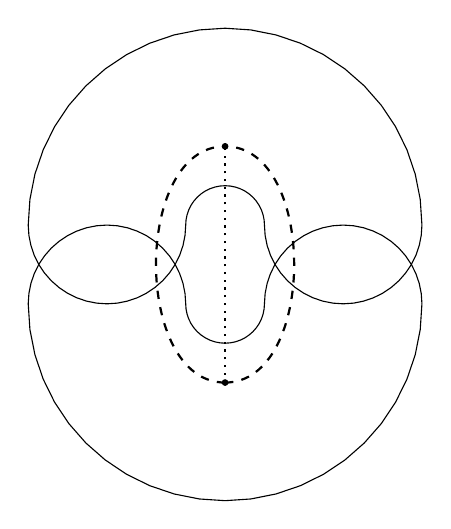
\begin{tikzpicture}[scale=0.5]
  \coordinate (u1) at (0,-3);
  \coordinate (u2) at (0,3);
  \draw[dotted,thick]
    (u1)
    --
    (u2);
  \draw[dashed,thick]
    (u1)
    to[bend left=90]
    (u2);
  \draw[dashed,thick]
    (u1)
    to[bend right=90]
    (u2);
  \draw[domain=0:180]
    plot
    ({cos(\x)},{sin(\x)+1});
  \draw[domain=0:180]
    plot
    ({5*cos(\x)},{5*sin(\x)+1});
  \draw[domain=180:360]
    plot
    ({cos(\x)},{sin(\x)-1});
  \draw[domain=180:360]
    plot
    ({5*cos(\x)},{5*sin(\x)-1});
  \draw[domain=180:360]
    plot
    ({2*cos(\x)-3},{2*sin(\x)+1});
  \draw[domain=180:360]
    plot
    ({2*cos(\x)+3},{2*sin(\x)+1});
  \draw[domain=0:180]
    plot
    ({2*cos(\x)-3},{2*sin(\x)-1});
  \draw[domain=0:180]
    plot
    ({2*cos(\x)+3},{2*sin(\x)-1});
  \filldraw
    (u1)
    circle
    [radius=2pt];
  \filldraw
    (u2)
    circle
    [radius=2pt];
\end{tikzpicture}
\]
The dotted line is what we would traditionally get from an intersection with two path components. But actually it would be closer (it is even the same in this example) to the homotopy type (a circle) of the space covered by these two sets to take an edge for each path component of the intersection with the restriction that they have the same source and target. That is, the two dashed lines. The idea now is to take the neglected topological structure of the coproduct into account. This in particular means that we consider
\begin{align*}
  \coprod_{k \in K}
  \mathrm{i}_{U_{k}}
\end{align*}
as continuous function. Then we call the kernel pair groupoid
\begin{align*}
  \mathbf{G}_{\coprod_{k \in K}\mathrm{i}_{U_{k}}}[\mathbf{Top}]
\end{align*}
internal to $\mathbf{Top}$ the \textbf{\v{C}ech groupoid (for $\mathrm{cov}_{S}$ in $\mathbf{Top}$)}. The internal nerve
\begin{align*}
  \mathrm{n}_{\mathbf{G}_{\coprod_{k \in K}\mathrm{i}_{U_{k}}}[\mathbf{Top}]}
\end{align*}
is called \textbf{\v{C}ech nerve (of $\mathrm{cov}_{S}$ in $\mathbf{Top}$)}. More generally for a category $\mathbf{C}$ with pullbacks and a morphism $f_{12}$ we call the kernel pair groupoid
\begin{align*}
  \mathbf{G}_{f_{12}}[\mathbf{C}]
\end{align*}
the \textbf{\v{C}ech groupoid (for $f_{12}$ in $\mathbf{C}$)} and the internal nerve
\begin{align*}
  \mathrm{n}_{\mathbf{G}_{f_{12}}[\mathbf{C}]}
\end{align*}
the \textbf{\v{C}ech nerve (of $f_{12}$ in $\mathbf{C}$)}. Of course, the case where the domain $X_{1}$ of $f_{12}$ is obtained from something deserving the name {\glqq}cover{\grqq} might be more interesting but it seems that also non-cover cases are interesting or so. But now back to the $\mathbf{Top}$ case. Look at the simplicial space
\begin{align*}
  \mathrm{n}_{\mathbf{G}_{\coprod_{k \in K}\mathrm{i}_{U_{k}}}[\mathbf{Top}]}
\end{align*}
or more specifically at its $N$-simplices
\begin{align*}
  \mathrm{n}_{\mathbf{G}_{\coprod_{k \in K}\mathrm{i}_{U_{k}}}[\mathbf{Top}]}
  ([N])
\end{align*}
which is nothing but a topological space of which we can look at path components. For the sake of simplicity let us only look at the cases $N = 0,1,2$ which actually suffice in the $1$-categorical case. Well,
\begin{align*}
  \mathrm{n}_{\mathbf{G}_{\coprod_{k \in K}\mathrm{i}_{U_{k}}}[\mathbf{Top}]}
  ([0])
  &=
  \mathrm{ob}_{\mathbf{G}_{\coprod_{k \in K}\mathrm{i}_{U_{k}}}[\mathbf{Top}]}
  =
  \coprod_{k \in K}
  U_{k}
\end{align*}
which as set is just the set of pairs $(x,U_{k})$ with $x \in U_{k}$. And the set of path components of $\coprod_{k \in K} U_{k}$ as space is just the set consisting of the path components from all the $U_{k}$. Next look at
\begin{align*}
  \mathrm{n}_{\mathbf{G}_{\coprod_{k \in K}\mathrm{i}_{U_{k}}}[\mathbf{Top}]}
  ([1])
  &=
  \mathrm{Mor}_{\mathbf{G}_{\coprod_{k \in K}\mathrm{i}_{U_{k}}}[\mathbf{Top}]}
  =
  \left(
    \coprod_{k \in K}
    U_{k}
  \right)
  \times_{S}
  \left(
    \coprod_{k \in K}
    U_{k}
  \right)
\end{align*}
which consists of $3$-tuples
\begin{align*}
  \left(
    x,
    U_{k_{1}},
    U_{k_{2}}
  \right)
\end{align*}
such that both $x \in U_{k_{1}}$ and $x \in U_{k_{2}}$. 
\begin{align*}
  \left(
    x,
    U_{k_{1}},
    U_{k_{2}}
  \right)
\end{align*}
and
\begin{align*}
  \left(
    x^{\backprime},
    U_{k_{1}^{\backprime}},
    U_{k_{2}^{\backprime}}
  \right)
\end{align*}
are in the same path component if and only if
\begin{align*}
  U_{k_{1}}
  &=
  U_{k_{1}^{\backprime}}
  \\
  U_{k_{2}}
  &=
  U_{k_{2}^{\backprime}}
\end{align*}
and there is a path from $x$ to $x^{\backprime}$. This follows from the properties of the product, coproduct and subspace topology w.r.t. to path connectedness. This holds more generally in the sense that for some $n \geq 3$
\begin{align*}
  \left(
    x,
    U_{k_{1}},
    \ldots,
    U_{k_{n}}
  \right)
\end{align*}
and
\begin{align*}
  \left(
    x^{\backprime},
    U_{k_{1}^{\backprime}},
    \ldots,
    U_{k_{b}^{\backprime}}
  \right)
\end{align*}
are in the same path component if and only if
\begin{align*}
  U_{k_{1}}
  &=
  U_{k_{1}^{\backprime}}
  \\
  &\cdots
  \\
  U_{k_{n}}
  &=
  U_{k_{n}^{\backprime}}
\end{align*}
and there is a path from $x$ to $x^{\backprime}$. So taking path components of
\begin{align*}
  \mathrm{n}_{\mathbf{G}_{\coprod_{k \in K}\mathrm{i}_{U_{k}}}[\mathbf{Top}]}
\end{align*}
objectwise seems to result in a simplicial set\footnote{this is claimed in \cite{wiki-pedia0en}: nerve of a covering} with one vertex for each path component of the coproduct of all the $U_{k}$, one edge for each path component of each non-empty intersection and so on for higher simplices. Combinatorially, one might object here that one gets two edges for each path component of each non-empty intersection since
\begin{align*}
  \left(
    x,
    U_{k_{1}},
    U_{k_{2}}
  \right)
\end{align*}
and
\begin{align*}
  \left(
    x,
    U_{k_{2}},
    U_{k_{1}}
  \right)
\end{align*}
are not connected by a path and a priori we should fear that we get loops here. But geometrically these should be contractible since as paths in the \v{C}ech groupoid these $3$-tuples are inverse to each other, that is,
\begin{align*}
  \left(
    x,
    U_{k_{1}},
    U_{k_{2}},
    U_{k_{1}}
  \right)
\end{align*}
and
\begin{align*}
  \left(
    x,
    U_{k_{2}},
    U_{k_{1}},
    U_{k_{2}}
  \right)
\end{align*}
are identities. Thus, geometrically, this should not play a role for the homotopy type and we could hope that geometrically realizing the simplicial set obtained from taking objectwise path components of the \v{C}ech nerve of $\mathrm{cov}_{S}$ in $\mathbf{Top}$ is a nice approximation of the space $S$ ideally with the same homotopy type if the space and the cover are good enough. Here we are again at the point of a \textit{nerve theorem}. A version for the Alexandrov nerve seems to be contained in appendix G of chapter 4 of \cite{8b5861fc}. And with some goodwill, arguably the \v{C}ech nerve case, too. Since we assume the internal nerve as internal embedding (motivated from the simplicial set case) we would say that the \v{C}ech groupoid for a good cover is a nice approximation of the homotopy type. What we actually want to drive at is a version of a \v{C}ech groupoid $\check{C}(\lbrace U_{k} \rbrace)$ for a cover $\lbrace U_{k} \rbrace$ of some homotopy type $X$ internal to an $(\infty,1)$-topos ${}_{(\infty,1)}\mathbf{C}$ which is equivalent to $X$ in ${}_{(\infty,1)}\mathbf{C}$ for good covers $\lbrace U_{k} \rbrace$ of the homotopy type $X$. Then to calculate cohomology
\begin{align*}
  {}_{(\infty,1)}\mathbf{C}
  \left(
    X,
    A
  \right)
\end{align*}
it should suffice to determine
\begin{align*}
  {}_{(\infty,1)}\mathbf{C}
  \left(
    \check{C}(\lbrace U_{k} \rbrace),
    A
  \right)
\end{align*}
This seems to be done in \cite{a565d200} using the notion of \textit{$\infty$-anafunctors} which are due to Makkai on the way to a foundation of mathematics by higher category theory. Finally, we can again use \v{C}ech methods in the cohomology classification of $G$-principal bundles in the $(\infty,1)$-topos
 setting in very much the same style as we could in the traditional case. Let us stop here dicussing the \v{C}ech stuff further and just accept the ideas (we hope are correct).



\section{What's Next}
\label{sec:whatsnext}
%\nocite{797789bc}
%\nocite{a565d200}
%\nocite{0349e8ea}
%\nocite{78202e13}
This will be a rather short section. We just talk about some literature we think is needed to understand \cite{a565d200}. First we have some traditional stuff which most readers who have read so far will already know well enough.
\begin{enumerate}
\item[$\bullet$]
Differential geometry in the scope of Isham \cite{797789bc} (i.p. to understand connections more formally).
\item[$\bullet$]
Algebraic topology in the scope of Hatcher \cite{8b5861fc} and maybe the fiber/cofiber sequence part of May \cite{78202e13} (for a better feeling on homotopy and maybe cohomology).
\item[$\bullet$]
Sheaf and topos theory in the scope of Mac Lane and Moerdijk \cite{c55c71e8}.
\end{enumerate}
Then one needs to understand this modern version of homotopy theory. For that purpose it seems reasonable to have a look at the following.
\begin{enumerate}
\item[$\bullet$]
Synthetic homotopy theory as homotopy type theory such as UFP-HoTT described in \cite{1ba1603e} with an eye on the foundations of mathematics\footnote{we do not know a really good single source for this}.
\item[$\bullet$]
$(\infty,1)$-categories and $(\infty,1)$-topoi in the scope of Lurie \cite{0349e8ea}.
\end{enumerate}
It may well be that the reading list is  not perfect and should be improved by someone who really read and understood \cite{a565d200}. So don't blame us for the potentially flawed and certainly to some extent incomplete list.
\\\\
As last word on these notes we should resolve if the titles initial and terminal context are serious. As you might have realized we like footnotes and to not directly spoil our result we write the answer in a footnote.\footnote{well, if the titles were serious then what we did in these notes would (up to coherent equivalence) be the only way ({\glqq}directed path{\grqq}) to go from chapter \ref{chap:initcontext} to chapter \ref{chap:termcontext} and we claim it is impossible to seriously claim this - hence regard it a pun}




\newpage



\nocite{c55c71e8}
\nocite{e837ef86}
\nocite{dc6f686f}
\nocite{1ba1603e}
\nocite{52fbba46}
\nocite{8b5861fc}
\nocite{wiki-nlab0000}
\nocite{wiki-pedia0en}

\bibliographystyle{alpha}
\bibliography{bib}



\appendix
\chapter{Tarski-Grothendieck Set Theory}
\label{chap:tg}
\stepcounter{prpcounter}
In this appendix chapter we want to explain what we mean by Tarski-Grothendieck set theory (abbr. TG). TG is actually very much like Zermelo-Fraenkel set theory with choice (abbr. ZFC) - that is, just ordinary mathematics as you know it - with the difference that one demands sets which behave a bit like ZFC. The sets we are talking about are \textit{Grothendieck universes} and each Grothendieck universe can be considered a place to do mathematics. The main purpose of universes is to conveniently avoid size issues (Russel's paradox): usually one works within a Grothendieck universe and if things inside this universe become to large then, no problem, we just go to a larger universe. Or something like that. We proceed in the following way. First we formally write down the axioms of ZFC but with an informal explanation. Then we define Grothendieck universes in a semi-formal way and then we will say what one has to demand in addition to ZFC to get TG. A full formalization of TG can be found on \href{http://us.metamath.org/mpeuni/mmset.html}{Metamath}. But also look at the according \cite{wiki-pedia0en} articles for more.
\\\\
ZFC is a formal system with the following axioms\footnote{statements assumed to be true} describing a mathematical universe of sets to some extent. Each point splits into
\begin{enumerate}
\item[$\bullet$]
an idea of what we want to describe in ordinary english
\item[$\bullet$]
a description of the idea in semi-formal english (using common mathematical symbols we should actually define in a formal way before using them)
\item[$\bullet$]
an actual (first-order) formula formalizing the idea
\end{enumerate}
Note that we use the symbols $x,x_{1},x_{2},\ldots$ plus $a,b,c,\ldots,x,y,z$ for variables for sets and that we write $x_{1} \in x_{2}$ for the {\glqq}is element of{\grqq} relation $\in(x_{1},x_{2})$. Moreover we tacitly applied some conventional precedence rules to get an easier to read version of the formula with less parentheses.
\begin{enumerate}
\item[(1)]
\begin{enumerate}
\item[$\bullet$]
The idea is that one should be able to compare sets for equality. Since one thinks of a set as being a collection of its elements it seems natural to consider two sets as the same if they have the same elements.
\item[$\bullet$]
Two sets $a,b$ are equal if $x \in a$ if and only if $x \in b$.
\item[$\bullet$]
Let $\mathcal{X}_{1}$ denote the formula
\begin{align*}
  \forall
  x
  .
  \left(
    x
    \in
    a
    \Leftrightarrow
    x
    \in
    b
  \right)
  \Rightarrow
  a
  =
  b
\end{align*}
In our setting $\mathcal{X}_{1}$ is called \textbf{axiom of extensionality}.
\end{enumerate}
\item[(2)]
\begin{enumerate}
\item[$\bullet$]
The idea is about how to specify certain elements of a set to build a new set containing exactly these specified elements. In other words, we want to be able to build subsets. So we want to assert that there is a set such that all elements of this set are all in some fixed set and all satisfy the same property.
\item[$\bullet$]
Given some suited formula $\mathcal{A}$ and a set $b$ then there is a set $a$ which precisely contains the members $x$ of $b$ for which $\mathcal{A}$ (we should perhaps write $\mathcal{A}(x)$) is true. One then usually uses so-called set-builder notation:
\begin{align*}
  a
  =
  \lbrace
      x
      \in
      b
    \vert
      \mathcal{A}(x)
  \rbrace
\end{align*}
\item[$\bullet$]
Let $\mathcal{A}$ denote a (well-formed) formula\footnote{a gramatically sensible expression (not necessarily true)} such that $a$ does not occur free\footnote{a variable occurs free in a formula if it is not quantified over it with either $\forall$ or $\exists$} in $\mathcal{A}$. Further let $\mathcal{X}_{2}$ denote the formula
\begin{align*}
  \exists
  a
  .
  \forall
  x
  .
  x
  \in
  a
  \Leftrightarrow
  x
  \in
  b
  \land
  \mathcal{A}
\end{align*}
In our setting $\mathcal{X}_{2}$ is called \textbf{axiom schema of specification}.
\end{enumerate}
\item[(3)]
\begin{enumerate}
\item[$\bullet$]
The idea is that given two sets we should have a set which contains these two sets as elements.
\item[$\bullet$]
For sets $x_{1},x_{2}$ we have a set $\lbrace x_{1},x_{2} \rbrace$.
\item[$\bullet$]
Let $\mathcal{X}_{3}$ denote the formula
\begin{align*}
  \exists
  p
  .
  x_{1}
  \in
  p
  \land
  x_{2}
  \in
  p
\end{align*}
In our setting $\mathcal{X}_{3}$ is called \textbf{axiom of pairing}.
\end{enumerate}
\item[(4)]
\begin{enumerate}
\item[$\bullet$]
The idea is that given a set we should have a set which contains all the elements of the elements in the given set as elements.
\item[$\bullet$]
Assume a set $l$ then there is a set
\begin{align*}
  u
  =:
  \bigcup_{s \in l}
  \lbrace
    x
    \in
    s
  \rbrace
\end{align*}
such that if $x$ is element of a member $s \in l$ then it is also element of $u$.
\item[$\bullet$]
Let $\mathcal{X}_{4}$ denote the formula
\begin{align*}
  \exists
  u
  .
  \forall
  x
  .
  \left(
    \exists
    s
    .
    x
    \in
    s
    \land
    s
    \in
    l
  \right)
  \Rightarrow
  x
  \in
  u
\end{align*}
In our setting $\mathcal{X}_{4}$ is called \textbf{axiom of union}.
\end{enumerate}
\item[(5)]
\begin{enumerate}
\item[$\bullet$]
The idea is that given a set we should have a set which contains all the subsets of the given one as elements.
\item[$\bullet$]
For a set $s$ there is a set $p =: \mathfrak{P}(s)$ such that if $a$ is a subset of $s$ then it is element of $p$.
\item[$\bullet$]
  Let $\mathcal{X}_{5}$ denote the formula
\begin{align*}
  \exists
  p
  .
  \forall
  a
  .
  \left(
    \forall
    x
    .
    x
    \in
    a
    \Rightarrow
    x
    \in
    s
  \right)
  \Rightarrow
  a
  \in
  p
\end{align*}
In our setting $\mathcal{X}_{5}$ is called \textbf{axiom of power set}.
\end{enumerate}
\item[(6)]
\begin{enumerate}
\item[$\bullet$]
The idea is to {\glqq}localize{\grqq} an induction principle into the set theory. This will implant a set of all natural numbers an hence in particular an infinite set. So we want to assert the existence of a set containing an element where the induction can start which is chosen to be the empty set - that is, the set such that any other set is not an element of it - and, by the induction principle: if given any element of this set there shall exist an element of this set containing exactly the given element and the elements of the given element. The so formed set does particularly contain a subset which behaves like the natural numbers. Namely the set with elements the empty set, the set with elements only the empty set, the set with elements only the empty set and the set with elements only the empty set, ... and so on. This can be understood as an encoding of 0,1,2,... and so on.
\item[$\bullet$]
There is a set $o$ which contains the emptyset $\emptyset$ and for each $i \in o$ we also have $i \cup \lbrace i \rbrace \in o$.
\item[$\bullet$]
Let $\mathcal{X}_{6}^{\textrm{a}}$ denote the formula
\begin{align*}
  \exists
  i
  .
  i
  \in
  o
  \land
  \forall
  x
  .
  \neg
  x
  \in
  i
\end{align*}
and let $\mathcal{X}_{6}^{\textrm{b}}$ denote the formula
\begin{align*}
  \forall
  i
  .
  i
  \in
  o
  \Rightarrow
  \exists
  u
  .
  u
  \in
  o
  \land
  \forall
  x
  .
  x
  \in
  u
  \Leftrightarrow
  x
  \in
  i
  \lor
  x
  =
  i
\end{align*}
Let further $\mathcal{X}_{6}$ denote the formula
\begin{align*}
  \exists
  o
  .
  (\mathcal{X}_{6}^{\textrm{a}})
  \land
  (\mathcal{X}_{6}^{\textrm{b}})
\end{align*}
In our setting $\mathcal{X}_{6}$ is called \textbf{axiom of infinity}.
\end{enumerate}
\item[(7)]
\begin{enumerate}
\item[$\bullet$]
The idea is that if some given set contains an element then it contains an element whose elements are all not elements of the given set. This ensures that sets are essentially well-founded trees and do in particular not contain themselves as element. In this context, note that $c \in p$ can be read as $c$ is a child of $p$.
\item[$\bullet$]
$a \neq \emptyset$ implies an $x$ in $a$ such that $x \cap a = \emptyset$.
\item[$\bullet$]
Let $\mathcal{X}_{7}$ denote the formula
\begin{align*}
  \left(
    \exists
    x
    .
    x
    \in
    a
  \right)
  \Rightarrow
  \exists
  x
  .
  x
  \in
  a
  \land
  \forall
  y
  .
  y
  \in
  x
  \Rightarrow
  \neg
  y
  \in
  a
\end{align*}
In our setting $\mathcal{X}_{7}$ is called \textbf{axiom of regularity}.
\end{enumerate}
\item[(8)]
\begin{enumerate}
\item[$\bullet$]
The idea is that a formula can serve as a mapping with domain a ll the sets under certain conditions and that, at least, when the mapping is restricted to a set its image must be so, too.
\item[$\bullet$]
Assume a formula $\mathcal{A}$. If for each element $x$ of a set $d$ there is precisely one set $p$ for which $\mathcal{A}$ is true then there is a set $i$ such that any element of $d$ implies an element of $i$ for which $\mathcal{A}$ is true.
\item[$\bullet$]
Let $\mathcal{A}$ be a formula such that $i$ is not free in $\mathcal{A}$. Then let $\mathcal{X}_{8}$ denote the formula
\begin{align*}
  \left(
    \forall
    x
    .
    x
    \in
    d
    \Rightarrow
    \exists!
    p
    .
    \mathcal{A}
  \right)
  \Rightarrow
  \exists
  i
  .
  \forall
  x
  .
  x
  \in
  d
  \Rightarrow
  \exists
  p
  .
  p
  \in
  i
  \land
  \mathcal{A}
\end{align*}
In our setting $\mathcal{X}_{8}$ is called \textbf{axiom schema of replacement}.
\end{enumerate}
\item[(9)]
\begin{enumerate}
\item[$\bullet$]
The idea is that if given a set of non-empty sets we should be able to choose precisely one element of each non-empty set in this collection to build a new set. While this seems intuitive at first glance since it holds in the finite case it is a bit magic: we can choose things but we do in general not know what we chose. Some consider this a bit unsatisfying on the philosophical level.
\item[$\bullet$]
Assume a set $l$. There is a set $c$ with the property that if we have a non-empty element $s$ of $l$ then there exist sets\footnote{we do not know which in general} $p \in s$ and $t = \lbrace s,p \rbrace$ such that $c$ is made up by all these $t$.
\item[$\bullet$]
Let $\tilde{\mathcal{X}}_{9}$ denote the formula
\begin{align*}
  \exists
  p
  .
  \forall
  x
  .
  \left(
    \exists
    t
    .
    \left(
      x
      \in
      s
      \land
      s
      \in
      t
    \right)
    \land
    \left(
      x
      \in
      t
      \land
      t
      \in
      c
    \right)
  \right)
  \Leftrightarrow
  x
  =
  p
\end{align*}
Let further $\mathcal{X}_{9}$ denote the formula
\begin{align*}
  \exists
  c
  .
  \forall
  e
  .
  \forall
  s
  .
  e
  \in
  s
  \land
  s
  \in
  l
  \Rightarrow
  \tilde{\mathcal{X}}_{9}
\end{align*}
In our setting $\mathcal{X}_{9}$ is called \textbf{axiom of choice}.
\end{enumerate}
\end{enumerate}
After having established ZFC let us turn to Grothendieck universes. For a Grothendieck universe to be sufficient to do some mathemathics it should as a set have the following features:
\begin{enumerate}
\item[(1)]
for an element of the universe each element of this element should be member of the universe
\item[(2)]
we should have an axiom of pairing inside the universe
\item[(3)]
we should have an axiom of union inside the universe
\item[(4)]
we should have an axiom of power set inside the universe
\end{enumerate}
So in semi-formal english: a set $\mathcal{U}$ is called \textbf{(Grothendieck) universe} if
\begin{enumerate}
\item[(GU1)]
$s \in \mathcal{U}$ and $x \in s$ implies $x \in \mathcal{U}$
\item[(GU2)]
$x_{1} \in \mathcal{U}$ and $x_{2} \in \mathcal{U}$ implies $\lbrace x_{1},x_{2} \rbrace \in \mathcal{U}$
\item[(GU3)]
Assume an element $K \in \mathcal{U}$ and for all $k \in K$ an element $x_{k} \in \mathcal{U}$. Then
\begin{align*}
  \bigcup_{k \in K}
  x_{k}
  &\in
  \mathcal{U}
\end{align*}
\item[(GU4)]
$x \in \mathcal{U}$ implies that the power set $\mathfrak{P}(x)$ of $x$ is in $\mathcal{U}$
\end{enumerate}
Note that a set $x$ which is member of the Grothendieck universe $\mathcal{U}$ is called \textbf{($\mathcal{U}$-)small}. In ZFC the only Grothendieck universe is $\emptyset$. But one could demand
\begin{enumerate}
\item[(TG)]
For every set $x$ there exists a Grothendieck universe $\mathcal{U}$ such that $x \in \mathcal{U}$
\end{enumerate}
The (first order) formula expressing (TG) is referred to as \textbf{Tarski's axiom}. ZFC together with Tarski's axiom is TG.


\end{document}
